\documentclass[12pt]{article}

\usepackage[margin=1in]{geometry}

\usepackage{float}

\usepackage[english]{babel}
\usepackage[utf8]{inputenc}
\usepackage{amsmath}
\usepackage{graphicx}
\usepackage[colorinlistoftodos]{todonotes}

\usepackage{caption}

\usepackage{textcomp}

\usepackage{rotating}

\usepackage{multirow,makecell}

\usepackage{dcolumn}
\newcolumntype{L}{D{.}{.}{1,1}}

\usepackage{adjustbox}
\usepackage{setspace}

\usepackage{longtable,lscape}

\usepackage{hyperref}

\usepackage{csquotes}
\usepackage[backend=bibtex,
            style=nature,
            sorting=none,
            autocite=superscript]{biblatex}
\addbibresource{references/biblio.bib}


\AtEveryBibitem{\clearfield{month}  \clearlist{language}}
\AtEveryCitekey{\clearfield{month}  \clearlist{language}}


\renewcommand{\baselinestretch}{2.0}

\renewcommand{\thefigure}{S\arabic{figure}}
\renewcommand{\thetable}{S\arabic{table}}



\begin{document}

\tableofcontents

\section{Supplementary methods}

\paragraph{Imputation of maternal education.} We imputed maternal education in the study sample jointly with all other variables, using the multiple chained imputation procedure implemented in the R package mi \cite{Su2011-he}. The data set for the imputation included all ca. 90,000 participants who had returned  either the first or the 3 year MoBa questionnaire, and all variables used in the final analysis plus additional variables deemed to be useful for imputation (details in lines 37-49 \href{https://github.com/gbiele/IPW/blob/master/AnalysisBIPW/021\_mi\_utils.R}{here}).

For the population data obtained from statistics Norway (SSB), two types of missing data needed to be imputed: 
\begin{enumerate}
	\item For small sub-groups, SSB did not provide counts for education subgroups with fewer than 5 members given a certain age-group and number of children (0.23\%). Instead SSB provided the total number of individuals in this subgroup and the next-largest education subgroup (with the same age and number of children). We re-redistributed the individuals with withhold education-level based on a negative-binomial regression of count on age group and number of children.
	\item After this first imputation step, we imputed the education-level for individuals for which SSB had no information about their education (3.9\%). We re-distributed, for each subgroup formed by maternal age-group and number of children, the individuals with unknown education to the educational levels, proportional to the frequency of the known educational levels. 
\end{enumerate}

\paragraph{Inverse probability weights} 
Inverse probability weights were calculated based on a hierarchical binomial regression, where participation rates were estimated as an effect of mothers' age, education, and parity.  The intercept as well as linear and non-linear (square) effects of mothers' age were allowed to vary by education and parity. 10-fold cross validation (using the package R package loo \cite{Vehtari2017-ne}) confirmed that this model did not over-fit the data. Following general recommendations we calculated stabilised weights \cite{Seaman2013-rj}. We calculated weights separately for imputed data sets and used a Two-Step Bayesian procedure \cite{Zigler2016-od} to incorporate uncertainty about weights into the regression analysis. That is, for each imputed data set we used the posterior distribution of model parameters and the data to calculate 2000 sets of participation probabilities, from which we then calculated 2000 sets of weights. During the estimation of the exposure outcome associations, which we again did for each of the 20 imputed data sets, we used for each iteration a new set of randomly chosen weights for the IPPW model. The weights for the IPPW model were always calculated based on the same data imputed data set used for the estimation of the association model.


\paragraph{Estimation of exposure outcome associations and lower bound selection bias magnitude} 
We implemented beta-binomial regression models in the probabilistic programming language Stan \cite{Carpenter2017-gd, Stan_Development_Team2017-lp}. The beta-binomial distribution is the natural choice for sum scores as outcome, which are bound between zero and an upper bound. Stan also allows simultaneous estimation of a regression model that uses inverse probability of participation weights (IPPW) and others that do not but adjusts for participation predictors (AR) or neither use weights not adjust (UR), while explicitly modeling the difference (bias) between the models' regression parameters.

\begin{table}
	\centering
	\begin{tabular}{lcccc}
		\hline
		& & \multicolumn{3}{c}{included variables} \\ \cline{3-5}
		Analysis & weights & exposure  & control  & particip. pred. \\ 
		\hline
		IPPW     &    +    &         +          &         +          & \\
		AR       &         &         +          &         +          &  + \\
		UR       &         &         +          &                   & \\
		\hline
	\end{tabular}
	\caption{Analysis models. IPPW = regression with inverse probability of participation weights. AR = regression with adjustment for confounders and participation predictors . UR = regression without adjustment. All regression models were estimated in a single Bayesian model.} 
	\label{tab:regmodels}
\end{table}

\paragraph{Comparison of exposure outcome association estimates} The statistical model directly estimates selection bias by modeling regression coefficients for AR (UR) as the coefficients for IPPW plus the difference between the IPPW and the AR (UR) coefficients. This approach accounts for covariation between regression weights when estimating bias. The ADHD sum scores are modeled as  $S = beta$-$binomial(\alpha,\beta)$, where $\alpha = \pi\phi$, $\beta = (1-\pi)\phi$, and $\phi$ is the over-dispersion parameter of the beta-binomial distribution. The expected proportion of the maximal sum score is 
\newline
$\mathbf{\pi}_{IPPW} = logit^{-1}(\mathbf{X} \beta_{IPPW})$ 
\newline
$\mathbf{\pi}_{AR} = logit^{-1}(\mathbf{X} \big( \beta_{IPPW} + \delta_{AR} \big) + \mathbf{P}\rho)$
\newline
where \textbf{X} is a matrix containing exposures of interest and adjustment variables excluding participation predictors, $\beta_{IPPW}$ are the regression weights for the IPPW analysis, $\delta_{AR}$ models the differences between regression weights for the weighted and adjusted regression, \textbf{P} and $\rho$ are participation predictors and corresponding regression weights. Further, the expected proportion of the maximal sum score for the UR regression is
\newline
$\mathbf{\pi}_{UR} = logit^{-1}(\mathbf{X^E} \big( \beta^E_{IPPW} + \delta_{UR} \big))$
\newline
where $^E$ indicates that only exposure but no adjustment variables are considered.

Because coefficients of a beta-binomial regressions are on the less intuitive multiplicative scale, we calculated average marginal effects ($AME$), the expected change in the outcome ADHD sum score for a one unit change of the exposure, and report results on this scale.

We test for bias by using a region of practical equivalence approach (ROPE)\cite{Kruschke2010-zi}, which checks if the highest density region of the bias estimates lies within a region of bias magnitudes that is for practical purposes equivalent with zero. This approach also allows quantifying the risk for substantial bias as the ratio of the posterior probabilities of the bias estimate being inside and outside the ROPE. More specifically, if $\delta_s$ is the posterior distribution of the standardised bias and $|\delta_s|$ its absolute value, then $RR_b =  \frac{P(|\delta_s|>0.5)}{P(|\delta_s|<0.5)}$. To put this statistic on the same scale as the better known log risk ratios, we can report the log of the risk ration, $log(RR_b)$, which can also directly be obtained as  $log(RR_b) = logit(P(|\delta_s|>0.5))$. 
More intuitively, the starting point for this statistic is that we can use posterior distributions from a Bayesian analysis to obtain the probability (Risk) that the bias-magnitude is inside or outside the interval from $-0.5$ to $+0.5$. By dividing these two probabilities, we obtain a risk ratio ($RR$) that the bias-magnitude ($RR_b$) is larger than 0.5. Finally, we take the logarithm of $RR_b$, which we call $log(RR_b)$. 

Which range of selection bias can be considered as unproblematic is best judged by subject matter experts. Alternatively, the bias estimate can be standardised by dividing it by the variance of the "gold standard" estimate \cite{Austin2009-xk}, here the IPPW estimate, which corrects selection bias. A complementary approach is to divide the bias estimate with the mean of the corrected estimate, capturing the intuition that deviations matter less if they are small compared to the corrected estimate. Based on previous literature \cite{Nilsen2009-ci, Austin2009-xk} We define the interval of $\pm$ 0.5 standardised deviations as practically equivalent with zero. This sets a high threshold for determining the presence of a problematic bias. In other contexts, different thresholds might be appropriate.

\paragraph{MCMC estimation} 
We used following priors:

\begin{itemize}
	\item $N(0,2)$ for intercepts and regression weights $\beta_{IPPW}$ and $\rho$
	\item improper ("noninformative") flat priors for the differences $\delta_{AR}$ and $\delta_{UR}$ between regression weights for the IPPW and AR or UR models.
	\item improper (uninformative) flat priors in the range $[0,1]$ for the logit of the the overdispersion parameters.
\end{itemize}


Regression models were estimated with Hamiltonian Monte Carlo sampling as implemented in Stan \cite{Stan_Development_Team2017-lp, Stan_Development_Team_2018-rs}. Per imputed data set we sampled three chains. Each chain consisted of 250 warmup samples and an additional 500 iterations that were used to calculate statistics. We checked convergence of the 3 chains per imputed data sets by insuring that \^{R} values were below 1.1 \cite{Gelman1992-jz}, and no divergent transitions had occurred \cite{Stan_Development_Team2016-pc}. All parameters of all models successfully converged, as indicated by \^{R} values below 1.1. We thus merged all chains prior to calculating statistics \cite{Zhou2010-li} such that reported results are based on 30,000 (20 imputed data sets $\cdot$ 3 chains $\cdot$ 500 iterations) combined post-warmup samples.

\newpage

\section{Supplementary tables}


\begin{table}[ht]
	\begin{center}
		\begin{tabular}{llr}
			\hline
			Variable group        & Phenotype \& reference           & N \\
			\hline
			Participation         & Years education\cite{Okbay2016-mg} 	   & 292\,000\\
			indicator             & Age at first birth\cite{Barban2016-fa}       & 125\,000\\
			\multicolumn{1}{c}{"} & Nr. children born\cite{Barban2016-fa}       & 125\,000\\
			Exposure              & Birth weight\cite{Horikoshi2016-hq}    & 143\,000\\
			\multicolumn{1}{c}{"} & Ever smoked\cite{Tob_Gen_Cons2010-se} & 75\,000\\
			\multicolumn{1}{c}{"} & Nr. cigarettes per day\cite{Tob_Gen_Cons2010-se} & 75\,000\\
			\multicolumn{1}{c}{"} & Alcohol use\cite{Clarke2017-xz}       & 112\,000\\
			\multicolumn{1}{c}{"} & Lifetime cannabis use\cite{Stringer2016-or}     & 32\,000\\
			\multicolumn{1}{c}{"} & Anxiety\cite{Otowa2016-uo}        & 31\,000\\
			\multicolumn{1}{c}{"} & Depressive symptoms\cite{Okbay2016-pj}        & 161\,000\\
			Outcome               & ADHD diagnosis\cite{Demontis2017-zu}     & 55\,000\\
			\hline
		\end{tabular}
	\end{center}
	\caption{Genome wide association studies on predictors of participation, exposures and outcome.}
	\label{tab:gwas}
\end{table}


{
	\setlength\tabcolsep{3pt}
	\renewcommand{\arraystretch}{0.6}
	\begin{longtable}{llrrrrrrrrr}
		\hline
		Phenotype 1 & Phenotype 2 & $r_G$ & $se(r_G)$ & $z(r_G)$ & $h^2_{p2}$ & $se(h^2_{p2})$ & $z(h^2_{p2})$ & $h^2_{p1}$ & $se(h^2_{p1})$ & $z(h^2_{p1})$ \\ 
		\hline
		\endhead
ADHD & Years education & -0.54 & 0.03 & -18.4 & 0.12 & 0.00 & 30.2 & 0.23 & 0.01 & 15.5 \\ 
  ADHD & Age at first birth & -0.62 & 0.04 & -14.7 & 0.08 & 0.01 & 14.6 & 0.23 & 0.01 & 15.5 \\ 
  ADHD & Num. childr. born & 0.36 & 0.07 & 5.3 & 0.03 & 0.00 & 9.9 & 0.23 & 0.01 & 15.5 \\ 
  ADHD & Birthweight & -0.14 & 0.04 & -3.6 & 0.13 & 0.01 & 15.7 & 0.23 & 0.01 & 15.5 \\ 
  ADHD & Alcohol use & -0.04 & 0.05 & -0.8 & 0.08 & 0.01 & 13.0 & 0.23 & 0.01 & 15.5 \\ 
  ADHD & Cigarettes per day & 0.41 & 0.10 & 4.2 & 0.03 & 0.01 & 4.3 & 0.23 & 0.01 & 15.5 \\ 
  ADHD & Ever smoked & 0.49 & 0.06 & 7.9 & 0.08 & 0.01 & 11.4 & 0.23 & 0.01 & 15.5 \\ 
  ADHD & Cannabis use & 0.32 & 0.07 & 4.5 & 0.09 & 0.02 & 5.5 & 0.23 & 0.01 & 15.5 \\ 
  ADHD & Substance abuse & 0.63 & 0.04 & 15.0 & 0.02 & 0.00 & 16.4 & 0.23 & 0.01 & 15.5 \\ 
  ADHD & Anxiety disorder & 0.27 & 0.14 & 1.9 & 0.06 & 0.03 & 2.5 & 0.23 & 0.01 & 15.5 \\ 
  ADHD & Depression sympt. & 0.45 & 0.05 & 8.5 & 0.05 & 0.00 & 12.8 & 0.23 & 0.01 & 15.5 \\ 
  Years education & Age at first birth & 0.72 & 0.03 & 27.9 & 0.08 & 0.01 & 14.6 & 0.12 & 0.00 & 30.2 \\ 
  Years education & Num. childr. born & -0.23 & 0.04 & -6.0 & 0.03 & 0.00 & 9.9 & 0.12 & 0.00 & 30.2 \\ 
  Years education & Birthweight & 0.11 & 0.03 & 4.3 & 0.13 & 0.01 & 15.7 & 0.12 & 0.00 & 30.2 \\ 
  Years education & Alcohol use & 0.18 & 0.03 & 5.9 & 0.08 & 0.01 & 13.0 & 0.12 & 0.00 & 30.2 \\ 
  Years education & Cigarettes per day & -0.26 & 0.06 & -4.3 & 0.03 & 0.01 & 4.3 & 0.12 & 0.00 & 30.2 \\ 
  Years education & Ever smoked & -0.35 & 0.04 & -9.1 & 0.08 & 0.01 & 11.4 & 0.12 & 0.00 & 30.2 \\ 
  Years education & Cannabis use & -0.04 & 0.05 & -0.9 & 0.09 & 0.02 & 5.5 & 0.12 & 0.00 & 30.2 \\ 
  Years education & Substance abuse & -0.53 & 0.03 & -18.0 & 0.02 & 0.00 & 16.4 & 0.12 & 0.00 & 30.2 \\ 
  Years education & Anxiety disorder & -0.31 & 0.09 & -3.5 & 0.06 & 0.03 & 2.5 & 0.12 & 0.00 & 30.2 \\ 
  Years education & Depression sympt. & -0.33 & 0.04 & -9.0 & 0.05 & 0.00 & 12.8 & 0.12 & 0.00 & 30.2 \\ 
  Age at first birth & Num. childr. born & -0.65 & 0.05 & -13.6 & 0.03 & 0.00 & 9.9 & 0.08 & 0.01 & 14.6 \\ 
  Age at first birth & Birthweight & 0.10 & 0.04 & 2.5 & 0.13 & 0.01 & 15.7 & 0.08 & 0.01 & 14.6 \\ 
  Age at first birth & Alcohol use & 0.11 & 0.05 & 2.3 & 0.08 & 0.01 & 13.0 & 0.08 & 0.01 & 14.6 \\ 
  Age at first birth & Cigarettes per day & -0.46 & 0.10 & -4.6 & 0.03 & 0.01 & 4.3 & 0.08 & 0.01 & 14.6 \\ 
  Age at first birth & Ever smoked & -0.37 & 0.05 & -7.3 & 0.08 & 0.01 & 11.4 & 0.08 & 0.01 & 14.6 \\ 
  Age at first birth & Cannabis use & -0.17 & 0.07 & -2.4 & 0.09 & 0.02 & 5.5 & 0.08 & 0.01 & 14.6 \\ 
  Age at first birth & Substance abuse & -0.62 & 0.05 & -13.4 & 0.02 & 0.00 & 16.4 & 0.08 & 0.01 & 14.6 \\ 
  Age at first birth & Anxiety disorder & -0.24 & 0.12 & -2.0 & 0.06 & 0.03 & 2.5 & 0.08 & 0.01 & 14.6 \\ 
  Age at first birth & Depression sympt. & -0.34 & 0.05 & -7.4 & 0.05 & 0.00 & 12.8 & 0.08 & 0.01 & 14.6 \\ 
  Num. childr. born & Birthweight & -0.03 & 0.05 & -0.5 & 0.13 & 0.01 & 15.7 & 0.03 & 0.00 & 9.9 \\ 
  Num. childr. born & Alcohol use & 0.06 & 0.06 & 1.0 & 0.08 & 0.01 & 13.0 & 0.03 & 0.00 & 9.9 \\ 
  Num. childr. born & Cigarettes per day & 0.16 & 0.10 & 1.5 & 0.03 & 0.01 & 4.3 & 0.03 & 0.00 & 9.9 \\ 
  Num. childr. born & Ever smoked & 0.08 & 0.07 & 1.3 & 0.08 & 0.01 & 11.4 & 0.03 & 0.00 & 9.9 \\ 
  Num. childr. born & Cannabis use & 0.05 & 0.10 & 0.5 & 0.09 & 0.02 & 5.5 & 0.03 & 0.00 & 9.9 \\ 
  Num. childr. born & Substance abuse & 0.33 & 0.06 & 5.6 & 0.02 & 0.00 & 16.4 & 0.03 & 0.00 & 9.9 \\ 
  Num. childr. born & Anxiety disorder & 0.20 & 0.17 & 1.2 & 0.06 & 0.03 & 2.5 & 0.03 & 0.00 & 9.9 \\ 
  Num. childr. born & Depression sympt. & 0.19 & 0.07 & 2.9 & 0.05 & 0.00 & 12.8 & 0.03 & 0.00 & 9.9 \\ 
  Birthweight & Alcohol use & -0.06 & 0.04 & -1.3 & 0.08 & 0.01 & 13.0 & 0.13 & 0.01 & 15.7 \\ 
  Birthweight & Cigarettes per day & -0.04 & 0.06 & -0.7 & 0.03 & 0.01 & 4.3 & 0.13 & 0.01 & 15.7 \\ 
  Birthweight & Ever smoked & 0.01 & 0.04 & 0.1 & 0.08 & 0.01 & 11.4 & 0.13 & 0.01 & 15.7 \\ 
  Birthweight & Cannabis use & -0.02 & 0.07 & -0.3 & 0.09 & 0.02 & 5.5 & 0.13 & 0.01 & 15.7 \\ 
  Birthweight & Substance abuse & -0.18 & 0.04 & -4.9 & 0.02 & 0.00 & 16.4 & 0.13 & 0.01 & 15.7 \\ 
  Birthweight & Anxiety disorder & -0.07 & 0.11 & -0.7 & 0.06 & 0.03 & 2.5 & 0.13 & 0.01 & 15.7 \\ 
  Birthweight & Depression sympt. & -0.07 & 0.04 & -1.7 & 0.05 & 0.00 & 12.8 & 0.13 & 0.01 & 15.7 \\ 
  Alcohol use & Cigarettes per day & -0.10 & 0.09 & -1.1 & 0.03 & 0.01 & 4.3 & 0.08 & 0.01 & 13.0 \\ 
  Alcohol use & Ever smoked & 0.40 & 0.06 & 6.3 & 0.08 & 0.01 & 11.4 & 0.08 & 0.01 & 13.0 \\ 
  Alcohol use & Cannabis use & 0.39 & 0.08 & 4.8 & 0.09 & 0.02 & 5.5 & 0.08 & 0.01 & 13.0 \\ 
  Alcohol use & Substance abuse & 0.18 & 0.05 & 3.9 & 0.02 & 0.00 & 16.4 & 0.08 & 0.01 & 13.0 \\ 
  Alcohol use & Anxiety disorder & 0.05 & 0.12 & 0.4 & 0.06 & 0.03 & 2.5 & 0.08 & 0.01 & 13.0 \\ 
  Alcohol use & Depression sympt. & -0.16 & 0.06 & -2.8 & 0.05 & 0.00 & 12.8 & 0.08 & 0.01 & 13.0 \\ 
  Cigarettes per day & Ever smoked & 0.37 & 0.11 & 3.5 & 0.08 & 0.01 & 11.4 & 0.03 & 0.01 & 4.3 \\ 
  Cigarettes per day & Cannabis use & 0.07 & 0.13 & 0.6 & 0.09 & 0.02 & 5.5 & 0.03 & 0.01 & 4.3 \\ 
  Cigarettes per day & Substance abuse & 0.50 & 0.08 & 5.9 & 0.02 & 0.00 & 16.4 & 0.03 & 0.01 & 4.3 \\ 
  Cigarettes per day & Anxiety disorder & -0.03 & 0.20 & -0.2 & 0.06 & 0.03 & 2.5 & 0.03 & 0.01 & 4.3 \\ 
  Cigarettes per day & Depression sympt. & 0.26 & 0.09 & 3.0 & 0.05 & 0.00 & 12.8 & 0.03 & 0.01 & 4.3 \\ 
  Ever smoked & Cannabis use & 0.68 & 0.10 & 6.5 & 0.09 & 0.02 & 5.5 & 0.08 & 0.01 & 11.4 \\ 
  Ever smoked & Substance abuse & 0.60 & 0.05 & 11.6 & 0.02 & 0.00 & 16.4 & 0.08 & 0.01 & 11.4 \\ 
  Ever smoked & Anxiety disorder & 0.58 & 0.16 & 3.5 & 0.06 & 0.03 & 2.5 & 0.08 & 0.01 & 11.4 \\ 
  Ever smoked & Depression sympt. & 0.25 & 0.06 & 4.4 & 0.05 & 0.00 & 12.8 & 0.08 & 0.01 & 11.4 \\ 
  Cannabis use & Substance abuse & 0.30 & 0.08 & 4.0 & 0.02 & 0.00 & 16.4 & 0.09 & 0.02 & 5.5 \\ 
  Cannabis use & Anxiety disorder & -0.05 & 0.18 & -0.3 & 0.06 & 0.03 & 2.5 & 0.09 & 0.02 & 5.5 \\ 
  Cannabis use & Depression sympt. & 0.25 & 0.08 & 2.9 & 0.05 & 0.00 & 12.8 & 0.09 & 0.02 & 5.5 \\ 
  Substance abuse & Anxiety disorder & 0.31 & 0.13 & 2.5 & 0.06 & 0.03 & 2.5 & 0.02 & 0.00 & 16.4 \\ 
  Substance abuse & Depression sympt. & 0.50 & 0.06 & 9.1 & 0.05 & 0.00 & 12.8 & 0.02 & 0.00 & 16.4 \\ 
  Anxiety disorder & Depression sympt. & 0.65 & 0.17 & 3.9 & 0.05 & 0.00 & 12.8 & 0.06 & 0.03 & 2.5 \\ 
  \hline
  \caption{SNP based genetic correlations and heritability estimates from publicly available GWAS summary statistics.} 
  \label{tab:rg}
\end{longtable}
\renewcommand{\arraystretch}{1}
}

\begin{sidewaystable}
	
	
		\begin{tabular}{rLlLlLlLlLLlL}
\hline
& \multicolumn{2}{c}{$IPPW$} & 
\multicolumn{2}{c}{$AR$} &
\multicolumn{2}{c}{$\delta=AR-IPPW$} &
\multicolumn{3}{c}{$\delta/\sigma_{IPPW}$ } &
\multicolumn{3}{c}{$\delta/\mu_{IPPW}$ }  \\
&\multicolumn{1}{c}{\footnotesize m} & \multicolumn{1}{c}{\footnotesize HDI} &
\multicolumn{1}{c}{\footnotesize m} & \multicolumn{1}{c}{\footnotesize HDI} &
\multicolumn{1}{c}{\footnotesize m} & \multicolumn{1}{c}{\footnotesize HDI} &  
\multicolumn{1}{c}{\footnotesize m} & \multicolumn{2}{c}{\footnotesize HDI} {\footnotesize log(RR$_b$)} &
\multicolumn{1}{c}{\footnotesize m} & \multicolumn{2}{c}{\footnotesize HDI} {\footnotesize log(RR$_b$)} \\
\hline
small f. gest. age & 0.32 & (0.23,0.41) & 0.31 & (0.22,0.39) & 0.01 & (-0.11,0.13) & 0.27 & (-2.01,2.45) & -0.9 & 0.05 & (-0.34,0.41) & 3.4 \\
preterm & 0.16 & (0.04,0.28) & 0.13 & (0.01,0.23) & 0.04 & (-0.13,0.19) & 0.51 & (-1.76,2.69) & -1.0 & 0.22 & (-0.77,1.18) & 0.3 \\
m. drug use & 0.14 & (0.04,0.24) & 0.29 & (0.20,0.39) & -0.15 & (-0.28,-0.02) & -2.46 & (-4.62,-0.33) & -2.9 & -1.04 & (-1.96,-0.14) & -1.7 \\
m. drug use score & -0.14 & (-0.25,-0.03) & -0.01 & (-0.11,0.08) & -0.13 & (-0.25,-0.01) & -1.94 & (-3.87,-0.12) & -2.3 & -0.92 & (-1.84,-0.06) & -1.3 \\
m. LTH & 0.07 & (0.04,0.10) & 0.28 & (0.25,0.30) & -0.21 & (-0.25,-0.16) & -11 & (-12.69,-8.34) & -Inf & -3.06 & (-3.69,-2.42) & -Inf \\
m. SCL5 & 0.16 & (0.12,0.20) & 0.34 & (0.31,0.37) & -0.18 & (-0.22,-0.13) & -7.97 & (-9.98,-5.84) & -Inf & -1.12 & (-1.40,-0.82) & -7.7 \\
p. drug use & 0.14 & (0.04,0.25) & 0.08 & (0.00,0.15) & 0.06 & (-0.05,0.18) & 0.99 & (-0.74,2.87) & -1.2 & 0.44 & (-0.33,1.27) & 0.1 \\
p. drug use score & 0.12 & (0.02,0.22) & 0.08 & (0.01,0.16) & 0.03 & (-0.07,0.14) & 0.53 & (-1.22,2.28) & -0.7 & 0.28 & (-0.65,1.21) & 0.3 \\
m. smoking & 0.49 & (0.39,0.58) & 0.89 & (0.78,1.01) & -0.41 & (-0.56,-0.26) & -6.71 & (-9.16,-4.31) & -10.3 & -0.84 & (-1.14,-0.54) & -3.4 \\
m. num. cigarettes & 0.13 & (0.05,0.21) & 0.16 & (0.06,0.25) & -0.02 & (-0.15,0.10) & -0.50 & (-2.96,2.05) & -1.1 & -0.19 & (-1.11,0.76) & 0.4 \\
m. alc.  freq. & 0.08 & (-0.01,0.17) & 0.22 & (0.14,0.29) & -0.14 & (-0.25,-0.03) & -2.44 & (-4.42,-0.47) & -3.0 & -1.73 & (-3.14,-0.34) & -2.6 \\
m. eff. units alc. & 0.03 & (0.00,0.07) & 0.07 & (0.04,0.10) & -0.04 & (-0.08,0.00) & -1.88 & (-3.95,0.21) & -2.1 & -1.06 & (-2.23,0.12) & -1.4 \\
p. smoking & -0.01 & (-0.09,0.08) & 0.16 & (0.09,0.23) & -0.17 & (-0.27,-0.06) & -3.35 & (-5.39,-1.24) & -4.5 & -17 & (-27.27,-6.29) & -6.2 \\
p. num. cigarettes & 0.00 & (-0.08,0.08) & -0.05 & (-0.11,0.01) & 0.05 & (-0.04,0.14) & 1.03 & (-0.91,2.98) & -1.3 & 37 & (-32.24,105.35) & -5.1 \\
p. alc.  freq. & 0.02 & (-0.02,0.07) & 0.01 & (-0.03,0.05) & 0.01 & (-0.03,0.06) & 0.47 & (-0.96,2.05) & -0.5 & 0.60 & (-1.24,2.63) & -0.9 \\
p. typ. units alc. & 0.08 & (0.05,0.12) & 0.15 & (0.12,0.18) & -0.07 & (-0.11,-0.02) & -3.03 & (-5.08,-0.85) & -3.9 & -0.81 & (-1.37,-0.23) & -1.5 \\

\hline
\end{tabular}

	\caption{Means and 90\% HDIs of exposures outcome associations and standardised bias of the UR results.
		$AME_{IPPW}$, $AME_{UR}$: Average marginal effects from IPPW, and UR models, respectively. $\sigma_{IPPW}$ and $\mu_{IPPW}$ are standard deviation and mean of the posterior distribution of the IPPW regression coefficients. } 
	\label{tab:estimates-UR}
\end{sidewaystable}
\newpage

\section{Supplementary figures}

\begin{figure}[H]
	\centering
	% Created by tikzDevice version 0.12 on 2019-01-16 14:48:27
% !TEX encoding = UTF-8 Unicode
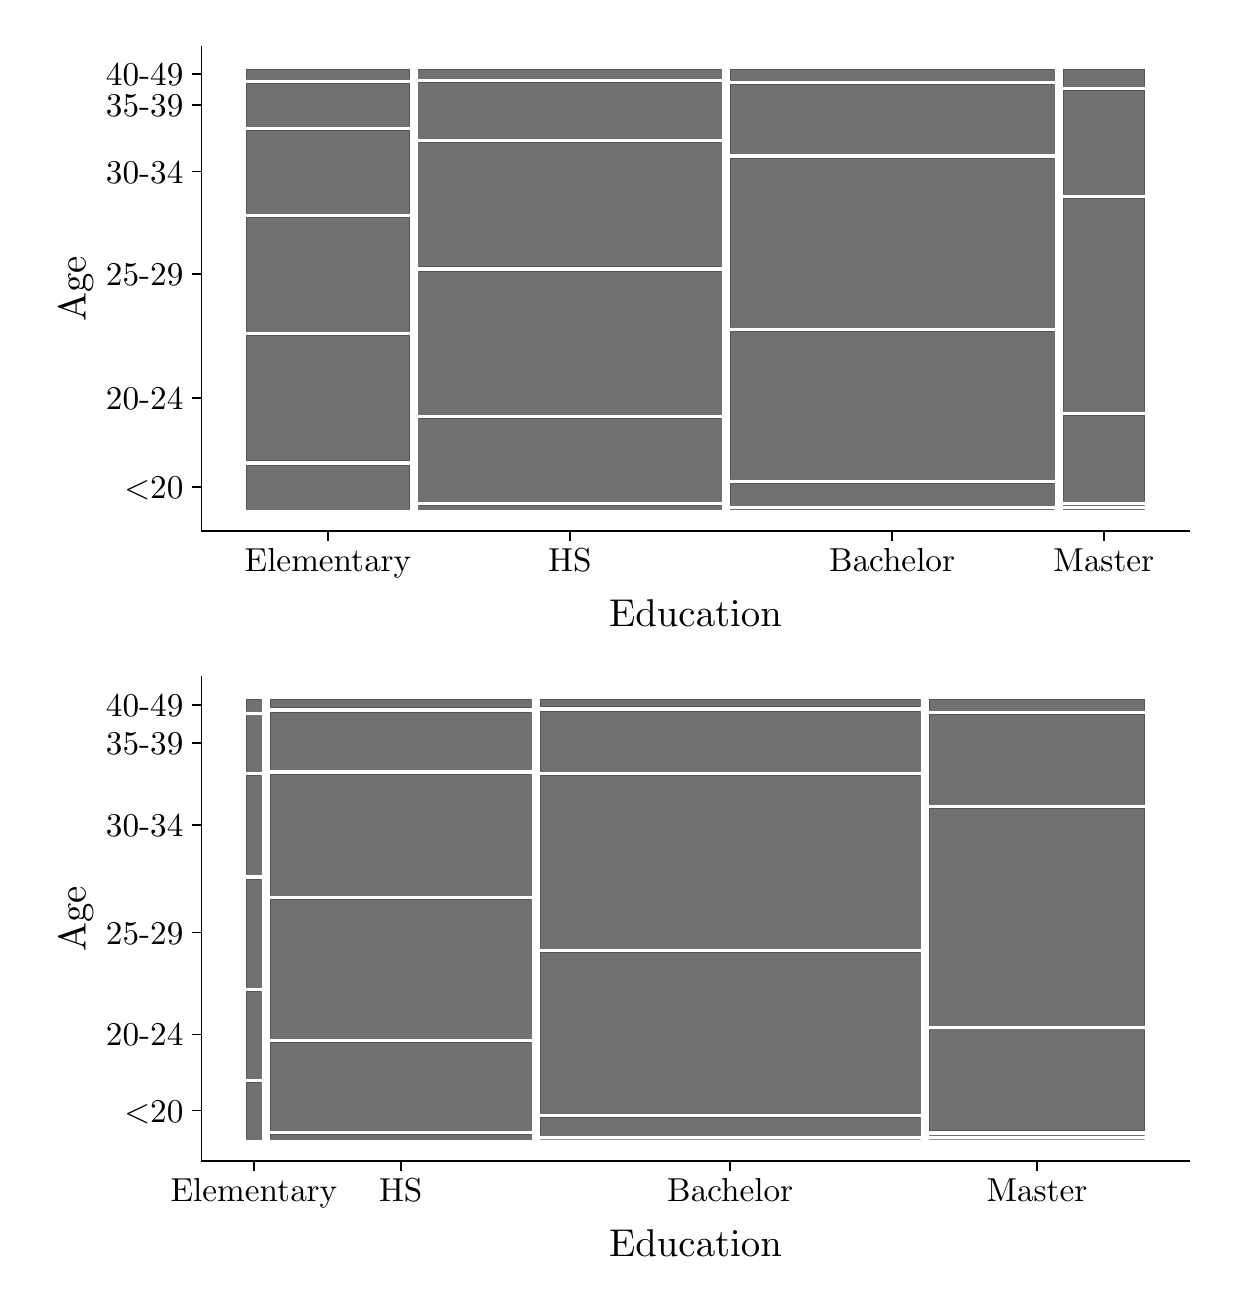
\begin{tikzpicture}[x=1pt,y=1pt]
\definecolor{fillColor}{RGB}{255,255,255}
\path[use as bounding box,fill=fillColor,fill opacity=0.00] (0,0) rectangle (426.79,455.24);
\begin{scope}
\path[clip] ( 62.78,273.33) rectangle (419.79,448.24);
\definecolor{drawColor}{RGB}{77,77,77}
\definecolor{fillColor}{RGB}{77,77,77}

\path[draw=drawColor,draw opacity=0.80,line width= 0.1pt,line join=round,fill=fillColor,fill opacity=0.80] ( 79.01,281.28) rectangle (138.02,297.28);

\path[draw=drawColor,draw opacity=0.80,line width= 0.1pt,line join=round,fill=fillColor,fill opacity=0.80] ( 79.01,298.80) rectangle (138.02,344.14);

\path[draw=drawColor,draw opacity=0.80,line width= 0.1pt,line join=round,fill=fillColor,fill opacity=0.80] ( 79.01,345.66) rectangle (138.02,386.76);

\path[draw=drawColor,draw opacity=0.80,line width= 0.1pt,line join=round,fill=fillColor,fill opacity=0.80] ( 79.01,388.28) rectangle (138.02,418.19);

\path[draw=drawColor,draw opacity=0.80,line width= 0.1pt,line join=round,fill=fillColor,fill opacity=0.80] ( 79.01,419.71) rectangle (138.02,435.09);

\path[draw=drawColor,draw opacity=0.80,line width= 0.1pt,line join=round,fill=fillColor,fill opacity=0.80] ( 79.01,436.60) rectangle (138.02,440.29);

\path[draw=drawColor,draw opacity=0.80,line width= 0.1pt,line join=round,fill=fillColor,fill opacity=0.80] (141.26,281.28) rectangle (250.54,282.64);

\path[draw=drawColor,draw opacity=0.80,line width= 0.1pt,line join=round,fill=fillColor,fill opacity=0.80] (141.26,284.15) rectangle (250.54,314.04);

\path[draw=drawColor,draw opacity=0.80,line width= 0.1pt,line join=round,fill=fillColor,fill opacity=0.80] (141.26,315.55) rectangle (250.54,367.38);

\path[draw=drawColor,draw opacity=0.80,line width= 0.1pt,line join=round,fill=fillColor,fill opacity=0.80] (141.26,368.90) rectangle (250.54,413.85);

\path[draw=drawColor,draw opacity=0.80,line width= 0.1pt,line join=round,fill=fillColor,fill opacity=0.80] (141.26,415.37) rectangle (250.54,435.46);

\path[draw=drawColor,draw opacity=0.80,line width= 0.1pt,line join=round,fill=fillColor,fill opacity=0.80] (141.26,436.98) rectangle (250.54,440.29);

\path[draw=drawColor,draw opacity=0.80,line width= 0.1pt,line join=round,fill=fillColor,fill opacity=0.80] (253.79,281.28) rectangle (370.94,281.28);

\path[draw=drawColor,draw opacity=0.80,line width= 0.1pt,line join=round,fill=fillColor,fill opacity=0.80] (253.79,282.79) rectangle (370.94,290.72);

\path[draw=drawColor,draw opacity=0.80,line width= 0.1pt,line join=round,fill=fillColor,fill opacity=0.80] (253.79,292.23) rectangle (370.94,345.68);

\path[draw=drawColor,draw opacity=0.80,line width= 0.1pt,line join=round,fill=fillColor,fill opacity=0.80] (253.79,347.20) rectangle (370.94,408.26);

\path[draw=drawColor,draw opacity=0.80,line width= 0.1pt,line join=round,fill=fillColor,fill opacity=0.80] (253.79,409.77) rectangle (370.94,434.88);

\path[draw=drawColor,draw opacity=0.80,line width= 0.1pt,line join=round,fill=fillColor,fill opacity=0.80] (253.79,436.40) rectangle (370.94,440.29);

\path[draw=drawColor,draw opacity=0.80,line width= 0.1pt,line join=round,fill=fillColor,fill opacity=0.80] (374.19,281.28) rectangle (403.56,281.28);

\path[draw=drawColor,draw opacity=0.80,line width= 0.1pt,line join=round,fill=fillColor,fill opacity=0.80] (374.19,282.79) rectangle (403.56,282.79);

\path[draw=drawColor,draw opacity=0.80,line width= 0.1pt,line join=round,fill=fillColor,fill opacity=0.80] (374.19,284.31) rectangle (403.56,315.26);

\path[draw=drawColor,draw opacity=0.80,line width= 0.1pt,line join=round,fill=fillColor,fill opacity=0.80] (374.19,316.78) rectangle (403.56,393.56);

\path[draw=drawColor,draw opacity=0.80,line width= 0.1pt,line join=round,fill=fillColor,fill opacity=0.80] (374.19,395.07) rectangle (403.56,432.71);

\path[draw=drawColor,draw opacity=0.80,line width= 0.1pt,line join=round,fill=fillColor,fill opacity=0.80] (374.19,434.23) rectangle (403.56,440.29);
\end{scope}
\begin{scope}
\path[clip] (  0.00,  0.00) rectangle (426.79,455.24);
\definecolor{drawColor}{RGB}{0,0,0}

\path[draw=drawColor,line width= 0.6pt,line join=round,line cap=rect] ( 62.78,273.33) --
	( 62.78,448.24);
\end{scope}
\begin{scope}
\path[clip] (  0.00,  0.00) rectangle (426.79,455.24);
\definecolor{drawColor}{RGB}{0,0,0}

\node[text=drawColor,anchor=base east,inner sep=0pt, outer sep=0pt, scale=  1.20] at ( 56.28,285.15) {\textless 20};

\node[text=drawColor,anchor=base east,inner sep=0pt, outer sep=0pt, scale=  1.20] at ( 56.28,317.34) {20-24};

\node[text=drawColor,anchor=base east,inner sep=0pt, outer sep=0pt, scale=  1.20] at ( 56.28,362.08) {25-29};

\node[text=drawColor,anchor=base east,inner sep=0pt, outer sep=0pt, scale=  1.20] at ( 56.28,399.10) {30-34};

\node[text=drawColor,anchor=base east,inner sep=0pt, outer sep=0pt, scale=  1.20] at ( 56.28,423.27) {35-39};

\node[text=drawColor,anchor=base east,inner sep=0pt, outer sep=0pt, scale=  1.20] at ( 56.28,434.32) {40-49};
\end{scope}
\begin{scope}
\path[clip] (  0.00,  0.00) rectangle (426.79,455.24);
\definecolor{drawColor}{RGB}{0,0,0}

\path[draw=drawColor,line width= 0.6pt,line join=round] ( 59.28,289.28) --
	( 62.78,289.28);

\path[draw=drawColor,line width= 0.6pt,line join=round] ( 59.28,321.47) --
	( 62.78,321.47);

\path[draw=drawColor,line width= 0.6pt,line join=round] ( 59.28,366.21) --
	( 62.78,366.21);

\path[draw=drawColor,line width= 0.6pt,line join=round] ( 59.28,403.23) --
	( 62.78,403.23);

\path[draw=drawColor,line width= 0.6pt,line join=round] ( 59.28,427.40) --
	( 62.78,427.40);

\path[draw=drawColor,line width= 0.6pt,line join=round] ( 59.28,438.45) --
	( 62.78,438.45);
\end{scope}
\begin{scope}
\path[clip] (  0.00,  0.00) rectangle (426.79,455.24);
\definecolor{drawColor}{RGB}{0,0,0}

\path[draw=drawColor,line width= 0.6pt,line join=round,line cap=rect] ( 62.78,273.33) --
	(419.79,273.33);
\end{scope}
\begin{scope}
\path[clip] (  0.00,  0.00) rectangle (426.79,455.24);
\definecolor{drawColor}{RGB}{0,0,0}

\path[draw=drawColor,line width= 0.6pt,line join=round] (108.51,269.83) --
	(108.51,273.33);

\path[draw=drawColor,line width= 0.6pt,line join=round] (195.90,269.83) --
	(195.90,273.33);

\path[draw=drawColor,line width= 0.6pt,line join=round] (312.36,269.83) --
	(312.36,273.33);

\path[draw=drawColor,line width= 0.6pt,line join=round] (388.87,269.83) --
	(388.87,273.33);
\end{scope}
\begin{scope}
\path[clip] (  0.00,  0.00) rectangle (426.79,455.24);
\definecolor{drawColor}{RGB}{0,0,0}

\node[text=drawColor,anchor=base,inner sep=0pt, outer sep=0pt, scale=  1.20] at (108.51,258.56) {Elementary};

\node[text=drawColor,anchor=base,inner sep=0pt, outer sep=0pt, scale=  1.20] at (195.90,258.56) {HS};

\node[text=drawColor,anchor=base,inner sep=0pt, outer sep=0pt, scale=  1.20] at (312.36,258.56) {Bachelor};

\node[text=drawColor,anchor=base,inner sep=0pt, outer sep=0pt, scale=  1.20] at (388.87,258.56) {Master};
\end{scope}
\begin{scope}
\path[clip] (  0.00,  0.00) rectangle (426.79,455.24);
\definecolor{drawColor}{RGB}{0,0,0}

\node[text=drawColor,anchor=base,inner sep=0pt, outer sep=0pt, scale=  1.40] at (241.29,238.95) {Education};
\end{scope}
\begin{scope}
\path[clip] (  0.00,  0.00) rectangle (426.79,455.24);
\definecolor{drawColor}{RGB}{0,0,0}

\node[text=drawColor,rotate= 90.00,anchor=base,inner sep=0pt, outer sep=0pt, scale=  1.40] at ( 20.97,360.79) {Age};
\end{scope}
\begin{scope}
\path[clip] ( 62.78, 45.70) rectangle (419.79,220.62);
\definecolor{drawColor}{RGB}{77,77,77}
\definecolor{fillColor}{RGB}{77,77,77}

\path[draw=drawColor,draw opacity=0.80,line width= 0.1pt,line join=round,fill=fillColor,fill opacity=0.80] ( 79.01, 53.66) rectangle ( 84.48, 74.14);

\path[draw=drawColor,draw opacity=0.80,line width= 0.1pt,line join=round,fill=fillColor,fill opacity=0.80] ( 79.01, 75.66) rectangle ( 84.48,107.18);

\path[draw=drawColor,draw opacity=0.80,line width= 0.1pt,line join=round,fill=fillColor,fill opacity=0.80] ( 79.01,108.70) rectangle ( 84.48,147.73);

\path[draw=drawColor,draw opacity=0.80,line width= 0.1pt,line join=round,fill=fillColor,fill opacity=0.80] ( 79.01,149.25) rectangle ( 84.48,185.23);

\path[draw=drawColor,draw opacity=0.80,line width= 0.1pt,line join=round,fill=fillColor,fill opacity=0.80] ( 79.01,186.75) rectangle ( 84.48,206.69);

\path[draw=drawColor,draw opacity=0.80,line width= 0.1pt,line join=round,fill=fillColor,fill opacity=0.80] ( 79.01,208.21) rectangle ( 84.48,212.67);

\path[draw=drawColor,draw opacity=0.80,line width= 0.1pt,line join=round,fill=fillColor,fill opacity=0.80] ( 87.72, 53.66) rectangle (181.87, 55.39);

\path[draw=drawColor,draw opacity=0.80,line width= 0.1pt,line join=round,fill=fillColor,fill opacity=0.80] ( 87.72, 56.91) rectangle (181.87, 88.54);

\path[draw=drawColor,draw opacity=0.80,line width= 0.1pt,line join=round,fill=fillColor,fill opacity=0.80] ( 87.72, 90.06) rectangle (181.87,140.25);

\path[draw=drawColor,draw opacity=0.80,line width= 0.1pt,line join=round,fill=fillColor,fill opacity=0.80] ( 87.72,141.76) rectangle (181.87,185.67);

\path[draw=drawColor,draw opacity=0.80,line width= 0.1pt,line join=round,fill=fillColor,fill opacity=0.80] ( 87.72,187.19) rectangle (181.87,208.05);

\path[draw=drawColor,draw opacity=0.80,line width= 0.1pt,line join=round,fill=fillColor,fill opacity=0.80] ( 87.72,209.57) rectangle (181.87,212.67);

\path[draw=drawColor,draw opacity=0.80,line width= 0.1pt,line join=round,fill=fillColor,fill opacity=0.80] (185.11, 53.66) rectangle (322.57, 53.66);

\path[draw=drawColor,draw opacity=0.80,line width= 0.1pt,line join=round,fill=fillColor,fill opacity=0.80] (185.11, 55.17) rectangle (322.57, 61.56);

\path[draw=drawColor,draw opacity=0.80,line width= 0.1pt,line join=round,fill=fillColor,fill opacity=0.80] (185.11, 63.07) rectangle (322.57,121.16);

\path[draw=drawColor,draw opacity=0.80,line width= 0.1pt,line join=round,fill=fillColor,fill opacity=0.80] (185.11,122.68) rectangle (322.57,185.24);

\path[draw=drawColor,draw opacity=0.80,line width= 0.1pt,line join=round,fill=fillColor,fill opacity=0.80] (185.11,186.75) rectangle (322.57,208.41);

\path[draw=drawColor,draw opacity=0.80,line width= 0.1pt,line join=round,fill=fillColor,fill opacity=0.80] (185.11,209.93) rectangle (322.57,212.67);

\path[draw=drawColor,draw opacity=0.80,line width= 0.1pt,line join=round,fill=fillColor,fill opacity=0.80] (325.82, 53.66) rectangle (403.56, 53.66);

\path[draw=drawColor,draw opacity=0.80,line width= 0.1pt,line join=round,fill=fillColor,fill opacity=0.80] (325.82, 55.17) rectangle (403.56, 55.17);

\path[draw=drawColor,draw opacity=0.80,line width= 0.1pt,line join=round,fill=fillColor,fill opacity=0.80] (325.82, 56.69) rectangle (403.56, 93.18);

\path[draw=drawColor,draw opacity=0.80,line width= 0.1pt,line join=round,fill=fillColor,fill opacity=0.80] (325.82, 94.70) rectangle (403.56,173.13);

\path[draw=drawColor,draw opacity=0.80,line width= 0.1pt,line join=round,fill=fillColor,fill opacity=0.80] (325.82,174.64) rectangle (403.56,207.19);

\path[draw=drawColor,draw opacity=0.80,line width= 0.1pt,line join=round,fill=fillColor,fill opacity=0.80] (325.82,208.70) rectangle (403.56,212.67);
\end{scope}
\begin{scope}
\path[clip] (  0.00,  0.00) rectangle (426.79,455.24);
\definecolor{drawColor}{RGB}{0,0,0}

\path[draw=drawColor,line width= 0.6pt,line join=round,line cap=rect] ( 62.78, 45.70) --
	( 62.78,220.62);
\end{scope}
\begin{scope}
\path[clip] (  0.00,  0.00) rectangle (426.79,455.24);
\definecolor{drawColor}{RGB}{0,0,0}

\node[text=drawColor,anchor=base east,inner sep=0pt, outer sep=0pt, scale=  1.20] at ( 56.28, 59.77) {\textless 20};

\node[text=drawColor,anchor=base east,inner sep=0pt, outer sep=0pt, scale=  1.20] at ( 56.28, 87.29) {20-24};

\node[text=drawColor,anchor=base east,inner sep=0pt, outer sep=0pt, scale=  1.20] at ( 56.28,124.08) {25-29};

\node[text=drawColor,anchor=base east,inner sep=0pt, outer sep=0pt, scale=  1.20] at ( 56.28,163.11) {30-34};

\node[text=drawColor,anchor=base east,inner sep=0pt, outer sep=0pt, scale=  1.20] at ( 56.28,192.59) {35-39};

\node[text=drawColor,anchor=base east,inner sep=0pt, outer sep=0pt, scale=  1.20] at ( 56.28,206.31) {40-49};
\end{scope}
\begin{scope}
\path[clip] (  0.00,  0.00) rectangle (426.79,455.24);
\definecolor{drawColor}{RGB}{0,0,0}

\path[draw=drawColor,line width= 0.6pt,line join=round] ( 59.28, 63.90) --
	( 62.78, 63.90);

\path[draw=drawColor,line width= 0.6pt,line join=round] ( 59.28, 91.42) --
	( 62.78, 91.42);

\path[draw=drawColor,line width= 0.6pt,line join=round] ( 59.28,128.22) --
	( 62.78,128.22);

\path[draw=drawColor,line width= 0.6pt,line join=round] ( 59.28,167.24) --
	( 62.78,167.24);

\path[draw=drawColor,line width= 0.6pt,line join=round] ( 59.28,196.72) --
	( 62.78,196.72);

\path[draw=drawColor,line width= 0.6pt,line join=round] ( 59.28,210.44) --
	( 62.78,210.44);
\end{scope}
\begin{scope}
\path[clip] (  0.00,  0.00) rectangle (426.79,455.24);
\definecolor{drawColor}{RGB}{0,0,0}

\path[draw=drawColor,line width= 0.6pt,line join=round,line cap=rect] ( 62.78, 45.70) --
	(419.79, 45.70);
\end{scope}
\begin{scope}
\path[clip] (  0.00,  0.00) rectangle (426.79,455.24);
\definecolor{drawColor}{RGB}{0,0,0}

\path[draw=drawColor,line width= 0.6pt,line join=round] ( 81.74, 42.20) --
	( 81.74, 45.70);

\path[draw=drawColor,line width= 0.6pt,line join=round] (134.79, 42.20) --
	(134.79, 45.70);

\path[draw=drawColor,line width= 0.6pt,line join=round] (253.84, 42.20) --
	(253.84, 45.70);

\path[draw=drawColor,line width= 0.6pt,line join=round] (364.69, 42.20) --
	(364.69, 45.70);
\end{scope}
\begin{scope}
\path[clip] (  0.00,  0.00) rectangle (426.79,455.24);
\definecolor{drawColor}{RGB}{0,0,0}

\node[text=drawColor,anchor=base,inner sep=0pt, outer sep=0pt, scale=  1.20] at ( 81.74, 30.94) {Elementary};

\node[text=drawColor,anchor=base,inner sep=0pt, outer sep=0pt, scale=  1.20] at (134.79, 30.94) {HS};

\node[text=drawColor,anchor=base,inner sep=0pt, outer sep=0pt, scale=  1.20] at (253.84, 30.94) {Bachelor};

\node[text=drawColor,anchor=base,inner sep=0pt, outer sep=0pt, scale=  1.20] at (364.69, 30.94) {Master};
\end{scope}
\begin{scope}
\path[clip] (  0.00,  0.00) rectangle (426.79,455.24);
\definecolor{drawColor}{RGB}{0,0,0}

\node[text=drawColor,anchor=base,inner sep=0pt, outer sep=0pt, scale=  1.40] at (241.29, 11.32) {Education};
\end{scope}
\begin{scope}
\path[clip] (  0.00,  0.00) rectangle (426.79,455.24);
\definecolor{drawColor}{RGB}{0,0,0}

\node[text=drawColor,rotate= 90.00,anchor=base,inner sep=0pt, outer sep=0pt, scale=  1.40] at ( 20.97,133.16) {Age};
\end{scope}
\end{tikzpicture}

	\caption{\footnotesize Mosaic plots of proportions of different sub-groups in the target population (top) and the study sample (bottom). The square-areas indicate what proportion of the total number belongs to different subgroups. HS = High school.}
	\label{fig:prop_moba_ssb}
\end{figure}

\begin{figure}[H]
	\centering
	% Created by tikzDevice version 0.12 on 2019-01-16 14:48:28
% !TEX encoding = UTF-8 Unicode
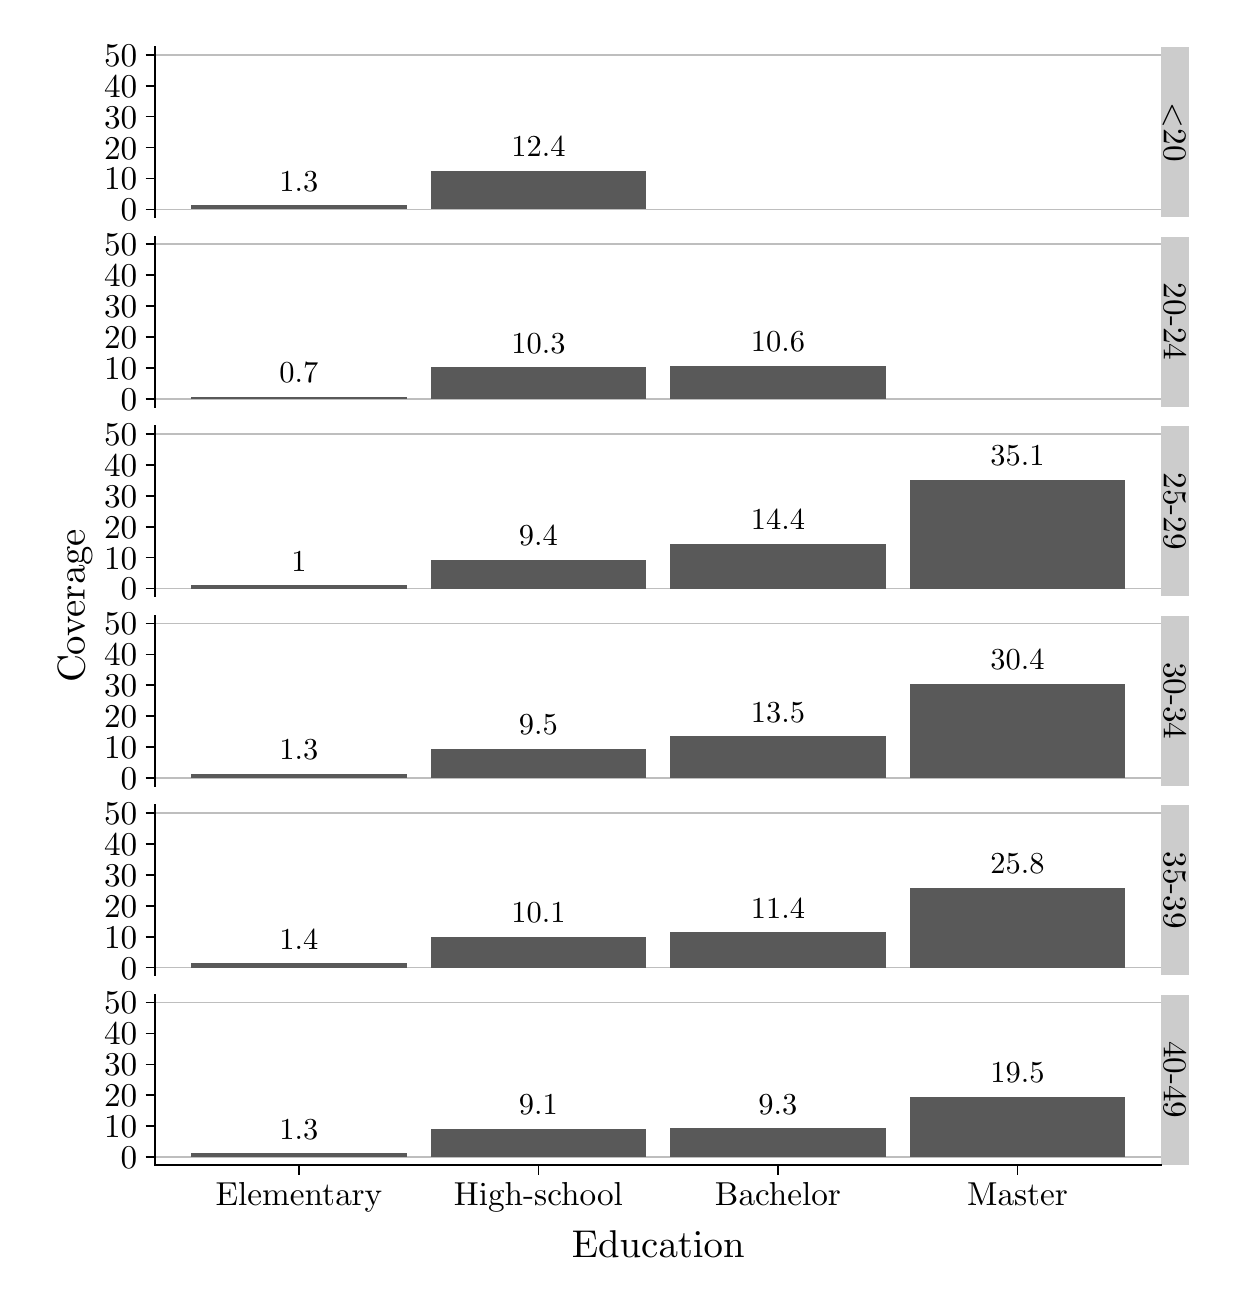
\begin{tikzpicture}[x=1pt,y=1pt]
\definecolor{fillColor}{RGB}{255,255,255}
\path[use as bounding box,fill=fillColor,fill opacity=0.00] (0,0) rectangle (426.79,455.24);
\begin{scope}
\path[clip] ( 46.08,386.75) rectangle (409.58,448.24);
\definecolor{drawColor}{RGB}{190,190,190}

\path[draw=drawColor,line width= 0.6pt,line join=round] ( 46.08,445.45) -- (409.58,445.45);

\path[draw=drawColor,line width= 0.6pt,line join=round] ( 46.08,389.55) -- (409.58,389.55);
\definecolor{fillColor}{gray}{0.35}

\path[fill=fillColor] ( 59.06,389.55) rectangle (136.96,391.04);

\path[fill=fillColor] (145.61,389.55) rectangle (223.50,403.38);
\definecolor{drawColor}{RGB}{0,0,0}

\node[text=drawColor,anchor=base,inner sep=0pt, outer sep=0pt, scale=  1.10] at ( 98.01,396.18) {1.3};

\node[text=drawColor,anchor=base,inner sep=0pt, outer sep=0pt, scale=  1.10] at (184.56,408.52) {12.4};
\end{scope}
\begin{scope}
\path[clip] ( 46.08,318.26) rectangle (409.58,379.75);
\definecolor{drawColor}{RGB}{190,190,190}

\path[draw=drawColor,line width= 0.6pt,line join=round] ( 46.08,376.96) -- (409.58,376.96);

\path[draw=drawColor,line width= 0.6pt,line join=round] ( 46.08,321.06) -- (409.58,321.06);
\definecolor{fillColor}{gray}{0.35}

\path[fill=fillColor] ( 59.06,321.06) rectangle (136.96,321.87);

\path[fill=fillColor] (145.61,321.06) rectangle (223.50,332.53);

\path[fill=fillColor] (232.16,321.06) rectangle (310.05,332.96);
\definecolor{drawColor}{RGB}{0,0,0}

\node[text=drawColor,anchor=base,inner sep=0pt, outer sep=0pt, scale=  1.10] at ( 98.01,327.01) {0.7};

\node[text=drawColor,anchor=base,inner sep=0pt, outer sep=0pt, scale=  1.10] at (184.56,337.68) {10.3};

\node[text=drawColor,anchor=base,inner sep=0pt, outer sep=0pt, scale=  1.10] at (271.11,338.10) {10.6};
\end{scope}
\begin{scope}
\path[clip] ( 46.08,249.77) rectangle (409.58,311.26);
\definecolor{drawColor}{RGB}{190,190,190}

\path[draw=drawColor,line width= 0.6pt,line join=round] ( 46.08,308.47) -- (409.58,308.47);

\path[draw=drawColor,line width= 0.6pt,line join=round] ( 46.08,252.56) -- (409.58,252.56);
\definecolor{fillColor}{gray}{0.35}

\path[fill=fillColor] ( 59.06,252.56) rectangle (136.96,253.67);

\path[fill=fillColor] (145.61,252.56) rectangle (223.50,263.06);

\path[fill=fillColor] (232.16,252.56) rectangle (310.05,268.61);

\path[fill=fillColor] (318.71,252.56) rectangle (396.60,291.83);
\definecolor{drawColor}{RGB}{0,0,0}

\node[text=drawColor,anchor=base,inner sep=0pt, outer sep=0pt, scale=  1.10] at ( 98.01,258.81) {1};

\node[text=drawColor,anchor=base,inner sep=0pt, outer sep=0pt, scale=  1.10] at (184.56,268.20) {9.4};

\node[text=drawColor,anchor=base,inner sep=0pt, outer sep=0pt, scale=  1.10] at (271.11,273.75) {14.4};

\node[text=drawColor,anchor=base,inner sep=0pt, outer sep=0pt, scale=  1.10] at (357.65,296.97) {35.1};
\end{scope}
\begin{scope}
\path[clip] ( 46.08,181.28) rectangle (409.58,242.77);
\definecolor{drawColor}{RGB}{190,190,190}

\path[draw=drawColor,line width= 0.6pt,line join=round] ( 46.08,239.97) -- (409.58,239.97);

\path[draw=drawColor,line width= 0.6pt,line join=round] ( 46.08,184.07) -- (409.58,184.07);
\definecolor{fillColor}{gray}{0.35}

\path[fill=fillColor] ( 59.06,184.07) rectangle (136.96,185.47);

\path[fill=fillColor] (145.61,184.07) rectangle (223.50,194.66);

\path[fill=fillColor] (232.16,184.07) rectangle (310.05,199.20);

\path[fill=fillColor] (318.71,184.07) rectangle (396.60,218.09);
\definecolor{drawColor}{RGB}{0,0,0}

\node[text=drawColor,anchor=base,inner sep=0pt, outer sep=0pt, scale=  1.10] at ( 98.01,190.62) {1.3};

\node[text=drawColor,anchor=base,inner sep=0pt, outer sep=0pt, scale=  1.10] at (184.56,199.80) {9.5};

\node[text=drawColor,anchor=base,inner sep=0pt, outer sep=0pt, scale=  1.10] at (271.11,204.34) {13.5};

\node[text=drawColor,anchor=base,inner sep=0pt, outer sep=0pt, scale=  1.10] at (357.65,223.23) {30.4};
\end{scope}
\begin{scope}
\path[clip] ( 46.08,112.78) rectangle (409.58,174.28);
\definecolor{drawColor}{RGB}{190,190,190}

\path[draw=drawColor,line width= 0.6pt,line join=round] ( 46.08,171.48) -- (409.58,171.48);

\path[draw=drawColor,line width= 0.6pt,line join=round] ( 46.08,115.58) -- (409.58,115.58);
\definecolor{fillColor}{gray}{0.35}

\path[fill=fillColor] ( 59.06,115.58) rectangle (136.96,117.09);

\path[fill=fillColor] (145.61,115.58) rectangle (223.50,126.83);

\path[fill=fillColor] (232.16,115.58) rectangle (310.05,128.32);

\path[fill=fillColor] (318.71,115.58) rectangle (396.60,144.38);
\definecolor{drawColor}{RGB}{0,0,0}

\node[text=drawColor,anchor=base,inner sep=0pt, outer sep=0pt, scale=  1.10] at ( 98.01,122.23) {1.4};

\node[text=drawColor,anchor=base,inner sep=0pt, outer sep=0pt, scale=  1.10] at (184.56,131.98) {10.1};

\node[text=drawColor,anchor=base,inner sep=0pt, outer sep=0pt, scale=  1.10] at (271.11,133.46) {11.4};

\node[text=drawColor,anchor=base,inner sep=0pt, outer sep=0pt, scale=  1.10] at (357.65,149.52) {25.8};
\end{scope}
\begin{scope}
\path[clip] ( 46.08, 44.29) rectangle (409.58,105.78);
\definecolor{drawColor}{RGB}{190,190,190}

\path[draw=drawColor,line width= 0.6pt,line join=round] ( 46.08,102.99) -- (409.58,102.99);

\path[draw=drawColor,line width= 0.6pt,line join=round] ( 46.08, 47.09) -- (409.58, 47.09);
\definecolor{fillColor}{gray}{0.35}

\path[fill=fillColor] ( 59.06, 47.09) rectangle (136.96, 48.50);

\path[fill=fillColor] (145.61, 47.09) rectangle (223.50, 57.24);

\path[fill=fillColor] (232.16, 47.09) rectangle (310.05, 57.49);

\path[fill=fillColor] (318.71, 47.09) rectangle (396.60, 68.87);
\definecolor{drawColor}{RGB}{0,0,0}

\node[text=drawColor,anchor=base,inner sep=0pt, outer sep=0pt, scale=  1.10] at ( 98.01, 53.64) {1.3};

\node[text=drawColor,anchor=base,inner sep=0pt, outer sep=0pt, scale=  1.10] at (184.56, 62.38) {9.1};

\node[text=drawColor,anchor=base,inner sep=0pt, outer sep=0pt, scale=  1.10] at (271.11, 62.63) {9.3};

\node[text=drawColor,anchor=base,inner sep=0pt, outer sep=0pt, scale=  1.10] at (357.65, 74.02) {19.5};
\end{scope}
\begin{scope}
\path[clip] (409.58,386.75) rectangle (419.79,448.24);
\definecolor{fillColor}{gray}{0.80}

\path[fill=fillColor] (409.58,386.75) rectangle (419.79,448.24);
\definecolor{drawColor}{RGB}{0,0,0}

\node[text=drawColor,rotate=-90.00,anchor=base,inner sep=0pt, outer sep=0pt, scale=  1.20] at (410.55,417.50) {\textless 20};
\end{scope}
\begin{scope}
\path[clip] (409.58,318.26) rectangle (419.79,379.75);
\definecolor{fillColor}{gray}{0.80}

\path[fill=fillColor] (409.58,318.26) rectangle (419.79,379.75);
\definecolor{drawColor}{RGB}{0,0,0}

\node[text=drawColor,rotate=-90.00,anchor=base,inner sep=0pt, outer sep=0pt, scale=  1.20] at (410.55,349.01) {20-24};
\end{scope}
\begin{scope}
\path[clip] (409.58,249.77) rectangle (419.79,311.26);
\definecolor{fillColor}{gray}{0.80}

\path[fill=fillColor] (409.58,249.77) rectangle (419.79,311.26);
\definecolor{drawColor}{RGB}{0,0,0}

\node[text=drawColor,rotate=-90.00,anchor=base,inner sep=0pt, outer sep=0pt, scale=  1.20] at (410.55,280.51) {25-29};
\end{scope}
\begin{scope}
\path[clip] (409.58,181.28) rectangle (419.79,242.77);
\definecolor{fillColor}{gray}{0.80}

\path[fill=fillColor] (409.58,181.28) rectangle (419.79,242.77);
\definecolor{drawColor}{RGB}{0,0,0}

\node[text=drawColor,rotate=-90.00,anchor=base,inner sep=0pt, outer sep=0pt, scale=  1.20] at (410.55,212.02) {30-34};
\end{scope}
\begin{scope}
\path[clip] (409.58,112.78) rectangle (419.79,174.28);
\definecolor{fillColor}{gray}{0.80}

\path[fill=fillColor] (409.58,112.78) rectangle (419.79,174.28);
\definecolor{drawColor}{RGB}{0,0,0}

\node[text=drawColor,rotate=-90.00,anchor=base,inner sep=0pt, outer sep=0pt, scale=  1.20] at (410.55,143.53) {35-39};
\end{scope}
\begin{scope}
\path[clip] (409.58, 44.29) rectangle (419.79,105.78);
\definecolor{fillColor}{gray}{0.80}

\path[fill=fillColor] (409.58, 44.29) rectangle (419.79,105.78);
\definecolor{drawColor}{RGB}{0,0,0}

\node[text=drawColor,rotate=-90.00,anchor=base,inner sep=0pt, outer sep=0pt, scale=  1.20] at (410.55, 75.04) {40-49};
\end{scope}
\begin{scope}
\path[clip] (  0.00,  0.00) rectangle (426.79,455.24);
\definecolor{drawColor}{RGB}{0,0,0}

\path[draw=drawColor,line width= 0.6pt,line join=round,line cap=rect] ( 46.08, 44.29) --
	(409.58, 44.29);
\end{scope}
\begin{scope}
\path[clip] (  0.00,  0.00) rectangle (426.79,455.24);
\definecolor{drawColor}{RGB}{0,0,0}

\path[draw=drawColor,line width= 0.6pt,line join=round] ( 98.01, 40.79) --
	( 98.01, 44.29);

\path[draw=drawColor,line width= 0.6pt,line join=round] (184.56, 40.79) --
	(184.56, 44.29);

\path[draw=drawColor,line width= 0.6pt,line join=round] (271.11, 40.79) --
	(271.11, 44.29);

\path[draw=drawColor,line width= 0.6pt,line join=round] (357.65, 40.79) --
	(357.65, 44.29);
\end{scope}
\begin{scope}
\path[clip] (  0.00,  0.00) rectangle (426.79,455.24);
\definecolor{drawColor}{RGB}{0,0,0}

\node[text=drawColor,anchor=base,inner sep=0pt, outer sep=0pt, scale=  1.20] at ( 98.01, 29.53) {Elementary};

\node[text=drawColor,anchor=base,inner sep=0pt, outer sep=0pt, scale=  1.20] at (184.56, 29.53) {High-school};

\node[text=drawColor,anchor=base,inner sep=0pt, outer sep=0pt, scale=  1.20] at (271.11, 29.53) {Bachelor};

\node[text=drawColor,anchor=base,inner sep=0pt, outer sep=0pt, scale=  1.20] at (357.65, 29.53) {Master};
\end{scope}
\begin{scope}
\path[clip] (  0.00,  0.00) rectangle (426.79,455.24);
\definecolor{drawColor}{RGB}{0,0,0}

\path[draw=drawColor,line width= 0.6pt,line join=round,line cap=rect] ( 46.08,386.75) --
	( 46.08,448.24);
\end{scope}
\begin{scope}
\path[clip] (  0.00,  0.00) rectangle (426.79,455.24);
\definecolor{drawColor}{RGB}{0,0,0}

\node[text=drawColor,anchor=base east,inner sep=0pt, outer sep=0pt, scale=  1.20] at ( 39.58,385.41) {0};

\node[text=drawColor,anchor=base east,inner sep=0pt, outer sep=0pt, scale=  1.20] at ( 39.58,396.60) {10};

\node[text=drawColor,anchor=base east,inner sep=0pt, outer sep=0pt, scale=  1.20] at ( 39.58,407.78) {20};

\node[text=drawColor,anchor=base east,inner sep=0pt, outer sep=0pt, scale=  1.20] at ( 39.58,418.96) {30};

\node[text=drawColor,anchor=base east,inner sep=0pt, outer sep=0pt, scale=  1.20] at ( 39.58,430.14) {40};

\node[text=drawColor,anchor=base east,inner sep=0pt, outer sep=0pt, scale=  1.20] at ( 39.58,441.32) {50};
\end{scope}
\begin{scope}
\path[clip] (  0.00,  0.00) rectangle (426.79,455.24);
\definecolor{drawColor}{RGB}{0,0,0}

\path[draw=drawColor,line width= 0.6pt,line join=round] ( 42.58,389.55) --
	( 46.08,389.55);

\path[draw=drawColor,line width= 0.6pt,line join=round] ( 42.58,400.73) --
	( 46.08,400.73);

\path[draw=drawColor,line width= 0.6pt,line join=round] ( 42.58,411.91) --
	( 46.08,411.91);

\path[draw=drawColor,line width= 0.6pt,line join=round] ( 42.58,423.09) --
	( 46.08,423.09);

\path[draw=drawColor,line width= 0.6pt,line join=round] ( 42.58,434.27) --
	( 46.08,434.27);

\path[draw=drawColor,line width= 0.6pt,line join=round] ( 42.58,445.45) --
	( 46.08,445.45);
\end{scope}
\begin{scope}
\path[clip] (  0.00,  0.00) rectangle (426.79,455.24);
\definecolor{drawColor}{RGB}{0,0,0}

\path[draw=drawColor,line width= 0.6pt,line join=round,line cap=rect] ( 46.08,318.26) --
	( 46.08,379.75);
\end{scope}
\begin{scope}
\path[clip] (  0.00,  0.00) rectangle (426.79,455.24);
\definecolor{drawColor}{RGB}{0,0,0}

\node[text=drawColor,anchor=base east,inner sep=0pt, outer sep=0pt, scale=  1.20] at ( 39.58,316.92) {0};

\node[text=drawColor,anchor=base east,inner sep=0pt, outer sep=0pt, scale=  1.20] at ( 39.58,328.10) {10};

\node[text=drawColor,anchor=base east,inner sep=0pt, outer sep=0pt, scale=  1.20] at ( 39.58,339.28) {20};

\node[text=drawColor,anchor=base east,inner sep=0pt, outer sep=0pt, scale=  1.20] at ( 39.58,350.46) {30};

\node[text=drawColor,anchor=base east,inner sep=0pt, outer sep=0pt, scale=  1.20] at ( 39.58,361.64) {40};

\node[text=drawColor,anchor=base east,inner sep=0pt, outer sep=0pt, scale=  1.20] at ( 39.58,372.82) {50};
\end{scope}
\begin{scope}
\path[clip] (  0.00,  0.00) rectangle (426.79,455.24);
\definecolor{drawColor}{RGB}{0,0,0}

\path[draw=drawColor,line width= 0.6pt,line join=round] ( 42.58,321.06) --
	( 46.08,321.06);

\path[draw=drawColor,line width= 0.6pt,line join=round] ( 42.58,332.24) --
	( 46.08,332.24);

\path[draw=drawColor,line width= 0.6pt,line join=round] ( 42.58,343.42) --
	( 46.08,343.42);

\path[draw=drawColor,line width= 0.6pt,line join=round] ( 42.58,354.60) --
	( 46.08,354.60);

\path[draw=drawColor,line width= 0.6pt,line join=round] ( 42.58,365.78) --
	( 46.08,365.78);

\path[draw=drawColor,line width= 0.6pt,line join=round] ( 42.58,376.96) --
	( 46.08,376.96);
\end{scope}
\begin{scope}
\path[clip] (  0.00,  0.00) rectangle (426.79,455.24);
\definecolor{drawColor}{RGB}{0,0,0}

\path[draw=drawColor,line width= 0.6pt,line join=round,line cap=rect] ( 46.08,249.77) --
	( 46.08,311.26);
\end{scope}
\begin{scope}
\path[clip] (  0.00,  0.00) rectangle (426.79,455.24);
\definecolor{drawColor}{RGB}{0,0,0}

\node[text=drawColor,anchor=base east,inner sep=0pt, outer sep=0pt, scale=  1.20] at ( 39.58,248.43) {0};

\node[text=drawColor,anchor=base east,inner sep=0pt, outer sep=0pt, scale=  1.20] at ( 39.58,259.61) {10};

\node[text=drawColor,anchor=base east,inner sep=0pt, outer sep=0pt, scale=  1.20] at ( 39.58,270.79) {20};

\node[text=drawColor,anchor=base east,inner sep=0pt, outer sep=0pt, scale=  1.20] at ( 39.58,281.97) {30};

\node[text=drawColor,anchor=base east,inner sep=0pt, outer sep=0pt, scale=  1.20] at ( 39.58,293.15) {40};

\node[text=drawColor,anchor=base east,inner sep=0pt, outer sep=0pt, scale=  1.20] at ( 39.58,304.33) {50};
\end{scope}
\begin{scope}
\path[clip] (  0.00,  0.00) rectangle (426.79,455.24);
\definecolor{drawColor}{RGB}{0,0,0}

\path[draw=drawColor,line width= 0.6pt,line join=round] ( 42.58,252.56) --
	( 46.08,252.56);

\path[draw=drawColor,line width= 0.6pt,line join=round] ( 42.58,263.74) --
	( 46.08,263.74);

\path[draw=drawColor,line width= 0.6pt,line join=round] ( 42.58,274.92) --
	( 46.08,274.92);

\path[draw=drawColor,line width= 0.6pt,line join=round] ( 42.58,286.10) --
	( 46.08,286.10);

\path[draw=drawColor,line width= 0.6pt,line join=round] ( 42.58,297.28) --
	( 46.08,297.28);

\path[draw=drawColor,line width= 0.6pt,line join=round] ( 42.58,308.47) --
	( 46.08,308.47);
\end{scope}
\begin{scope}
\path[clip] (  0.00,  0.00) rectangle (426.79,455.24);
\definecolor{drawColor}{RGB}{0,0,0}

\path[draw=drawColor,line width= 0.6pt,line join=round,line cap=rect] ( 46.08,181.28) --
	( 46.08,242.77);
\end{scope}
\begin{scope}
\path[clip] (  0.00,  0.00) rectangle (426.79,455.24);
\definecolor{drawColor}{RGB}{0,0,0}

\node[text=drawColor,anchor=base east,inner sep=0pt, outer sep=0pt, scale=  1.20] at ( 39.58,179.94) {0};

\node[text=drawColor,anchor=base east,inner sep=0pt, outer sep=0pt, scale=  1.20] at ( 39.58,191.12) {10};

\node[text=drawColor,anchor=base east,inner sep=0pt, outer sep=0pt, scale=  1.20] at ( 39.58,202.30) {20};

\node[text=drawColor,anchor=base east,inner sep=0pt, outer sep=0pt, scale=  1.20] at ( 39.58,213.48) {30};

\node[text=drawColor,anchor=base east,inner sep=0pt, outer sep=0pt, scale=  1.20] at ( 39.58,224.66) {40};

\node[text=drawColor,anchor=base east,inner sep=0pt, outer sep=0pt, scale=  1.20] at ( 39.58,235.84) {50};
\end{scope}
\begin{scope}
\path[clip] (  0.00,  0.00) rectangle (426.79,455.24);
\definecolor{drawColor}{RGB}{0,0,0}

\path[draw=drawColor,line width= 0.6pt,line join=round] ( 42.58,184.07) --
	( 46.08,184.07);

\path[draw=drawColor,line width= 0.6pt,line join=round] ( 42.58,195.25) --
	( 46.08,195.25);

\path[draw=drawColor,line width= 0.6pt,line join=round] ( 42.58,206.43) --
	( 46.08,206.43);

\path[draw=drawColor,line width= 0.6pt,line join=round] ( 42.58,217.61) --
	( 46.08,217.61);

\path[draw=drawColor,line width= 0.6pt,line join=round] ( 42.58,228.79) --
	( 46.08,228.79);

\path[draw=drawColor,line width= 0.6pt,line join=round] ( 42.58,239.97) --
	( 46.08,239.97);
\end{scope}
\begin{scope}
\path[clip] (  0.00,  0.00) rectangle (426.79,455.24);
\definecolor{drawColor}{RGB}{0,0,0}

\path[draw=drawColor,line width= 0.6pt,line join=round,line cap=rect] ( 46.08,112.78) --
	( 46.08,174.28);
\end{scope}
\begin{scope}
\path[clip] (  0.00,  0.00) rectangle (426.79,455.24);
\definecolor{drawColor}{RGB}{0,0,0}

\node[text=drawColor,anchor=base east,inner sep=0pt, outer sep=0pt, scale=  1.20] at ( 39.58,111.45) {0};

\node[text=drawColor,anchor=base east,inner sep=0pt, outer sep=0pt, scale=  1.20] at ( 39.58,122.63) {10};

\node[text=drawColor,anchor=base east,inner sep=0pt, outer sep=0pt, scale=  1.20] at ( 39.58,133.81) {20};

\node[text=drawColor,anchor=base east,inner sep=0pt, outer sep=0pt, scale=  1.20] at ( 39.58,144.99) {30};

\node[text=drawColor,anchor=base east,inner sep=0pt, outer sep=0pt, scale=  1.20] at ( 39.58,156.17) {40};

\node[text=drawColor,anchor=base east,inner sep=0pt, outer sep=0pt, scale=  1.20] at ( 39.58,167.35) {50};
\end{scope}
\begin{scope}
\path[clip] (  0.00,  0.00) rectangle (426.79,455.24);
\definecolor{drawColor}{RGB}{0,0,0}

\path[draw=drawColor,line width= 0.6pt,line join=round] ( 42.58,115.58) --
	( 46.08,115.58);

\path[draw=drawColor,line width= 0.6pt,line join=round] ( 42.58,126.76) --
	( 46.08,126.76);

\path[draw=drawColor,line width= 0.6pt,line join=round] ( 42.58,137.94) --
	( 46.08,137.94);

\path[draw=drawColor,line width= 0.6pt,line join=round] ( 42.58,149.12) --
	( 46.08,149.12);

\path[draw=drawColor,line width= 0.6pt,line join=round] ( 42.58,160.30) --
	( 46.08,160.30);

\path[draw=drawColor,line width= 0.6pt,line join=round] ( 42.58,171.48) --
	( 46.08,171.48);
\end{scope}
\begin{scope}
\path[clip] (  0.00,  0.00) rectangle (426.79,455.24);
\definecolor{drawColor}{RGB}{0,0,0}

\path[draw=drawColor,line width= 0.6pt,line join=round,line cap=rect] ( 46.08, 44.29) --
	( 46.08,105.78);
\end{scope}
\begin{scope}
\path[clip] (  0.00,  0.00) rectangle (426.79,455.24);
\definecolor{drawColor}{RGB}{0,0,0}

\node[text=drawColor,anchor=base east,inner sep=0pt, outer sep=0pt, scale=  1.20] at ( 39.58, 42.96) {0};

\node[text=drawColor,anchor=base east,inner sep=0pt, outer sep=0pt, scale=  1.20] at ( 39.58, 54.14) {10};

\node[text=drawColor,anchor=base east,inner sep=0pt, outer sep=0pt, scale=  1.20] at ( 39.58, 65.32) {20};

\node[text=drawColor,anchor=base east,inner sep=0pt, outer sep=0pt, scale=  1.20] at ( 39.58, 76.50) {30};

\node[text=drawColor,anchor=base east,inner sep=0pt, outer sep=0pt, scale=  1.20] at ( 39.58, 87.68) {40};

\node[text=drawColor,anchor=base east,inner sep=0pt, outer sep=0pt, scale=  1.20] at ( 39.58, 98.86) {50};
\end{scope}
\begin{scope}
\path[clip] (  0.00,  0.00) rectangle (426.79,455.24);
\definecolor{drawColor}{RGB}{0,0,0}

\path[draw=drawColor,line width= 0.6pt,line join=round] ( 42.58, 47.09) --
	( 46.08, 47.09);

\path[draw=drawColor,line width= 0.6pt,line join=round] ( 42.58, 58.27) --
	( 46.08, 58.27);

\path[draw=drawColor,line width= 0.6pt,line join=round] ( 42.58, 69.45) --
	( 46.08, 69.45);

\path[draw=drawColor,line width= 0.6pt,line join=round] ( 42.58, 80.63) --
	( 46.08, 80.63);

\path[draw=drawColor,line width= 0.6pt,line join=round] ( 42.58, 91.81) --
	( 46.08, 91.81);

\path[draw=drawColor,line width= 0.6pt,line join=round] ( 42.58,102.99) --
	( 46.08,102.99);
\end{scope}
\begin{scope}
\path[clip] (  0.00,  0.00) rectangle (426.79,455.24);
\definecolor{drawColor}{RGB}{0,0,0}

\node[text=drawColor,anchor=base,inner sep=0pt, outer sep=0pt, scale=  1.40] at (227.83, 10.97) {Education};
\end{scope}
\begin{scope}
\path[clip] (  0.00,  0.00) rectangle (426.79,455.24);
\definecolor{drawColor}{RGB}{0,0,0}

\node[text=drawColor,rotate= 90.00,anchor=base,inner sep=0pt, outer sep=0pt, scale=  1.40] at ( 20.61,246.27) {Coverage};
\end{scope}
\end{tikzpicture}

	\caption{\footnotesize Percent of the target population included in the study sample, stratified by maternal age and education. $Coverage = N_{study sample}/N_{target population}$.}
	\label{fig:coverage}
\end{figure}


\begin{figure}[H]
	\centering
	% Created by tikzDevice version 0.11 on 2018-03-23 13:16:34
% !TEX encoding = UTF-8 Unicode
\begin{tikzpicture}[x=1pt,y=1pt]
\definecolor{fillColor}{RGB}{255,255,255}
\path[use as bounding box,fill=fillColor,fill opacity=0.00] (0,0) rectangle (341.43,199.17);
\begin{scope}
\path[clip] (  0.00,  0.00) rectangle (341.43,199.17);
\definecolor{drawColor}{RGB}{0,0,0}

\node[text=drawColor,anchor=base,inner sep=0pt, outer sep=0pt, scale=  1.00] at (182.72,  2.40) {ADHD sum score};

\node[text=drawColor,rotate= 90.00,anchor=base,inner sep=0pt, outer sep=0pt, scale=  1.00] at (  9.60,117.58) {Frequency};
\end{scope}
\begin{scope}
\path[clip] (  0.00,  0.00) rectangle (341.43,199.17);
\definecolor{drawColor}{RGB}{0,0,0}

\path[draw=drawColor,line width= 0.4pt,line join=round,line cap=round] ( 52.77, 36.00) -- (289.03, 36.00);

\path[draw=drawColor,line width= 0.4pt,line join=round,line cap=round] ( 52.77, 36.00) -- ( 52.77, 34.37);

\path[draw=drawColor,line width= 0.4pt,line join=round,line cap=round] (111.84, 36.00) -- (111.84, 34.37);

\path[draw=drawColor,line width= 0.4pt,line join=round,line cap=round] (170.90, 36.00) -- (170.90, 34.37);

\path[draw=drawColor,line width= 0.4pt,line join=round,line cap=round] (229.97, 36.00) -- (229.97, 34.37);

\path[draw=drawColor,line width= 0.4pt,line join=round,line cap=round] (289.03, 36.00) -- (289.03, 34.37);

\node[text=drawColor,anchor=base,inner sep=0pt, outer sep=0pt, scale=  1.00] at ( 52.77, 18.00) {0};

\node[text=drawColor,anchor=base,inner sep=0pt, outer sep=0pt, scale=  1.00] at (111.84, 18.00) {5};

\node[text=drawColor,anchor=base,inner sep=0pt, outer sep=0pt, scale=  1.00] at (170.90, 18.00) {10};

\node[text=drawColor,anchor=base,inner sep=0pt, outer sep=0pt, scale=  1.00] at (229.97, 18.00) {15};

\node[text=drawColor,anchor=base,inner sep=0pt, outer sep=0pt, scale=  1.00] at (289.03, 18.00) {20};

\path[draw=drawColor,line width= 0.4pt,line join=round,line cap=round] ( 36.00, 42.04) -- ( 36.00,185.45);

\path[draw=drawColor,line width= 0.4pt,line join=round,line cap=round] ( 36.00, 42.04) -- ( 34.37, 42.04);

\path[draw=drawColor,line width= 0.4pt,line join=round,line cap=round] ( 36.00, 65.95) -- ( 34.37, 65.95);

\path[draw=drawColor,line width= 0.4pt,line join=round,line cap=round] ( 36.00, 89.85) -- ( 34.37, 89.85);

\path[draw=drawColor,line width= 0.4pt,line join=round,line cap=round] ( 36.00,113.75) -- ( 34.37,113.75);

\path[draw=drawColor,line width= 0.4pt,line join=round,line cap=round] ( 36.00,137.65) -- ( 34.37,137.65);

\path[draw=drawColor,line width= 0.4pt,line join=round,line cap=round] ( 36.00,161.55) -- ( 34.37,161.55);

\path[draw=drawColor,line width= 0.4pt,line join=round,line cap=round] ( 36.00,185.45) -- ( 34.37,185.45);

\node[text=drawColor,rotate= 90.00,anchor=base,inner sep=0pt, outer sep=0pt, scale=  1.00] at ( 25.20, 42.04) {0};

\node[text=drawColor,rotate= 90.00,anchor=base,inner sep=0pt, outer sep=0pt, scale=  1.00] at ( 25.20, 65.95) {1000};

\node[text=drawColor,rotate= 90.00,anchor=base,inner sep=0pt, outer sep=0pt, scale=  1.00] at ( 25.20,113.75) {3000};

\node[text=drawColor,rotate= 90.00,anchor=base,inner sep=0pt, outer sep=0pt, scale=  1.00] at ( 25.20,161.55) {5000};
\end{scope}
\begin{scope}
\path[clip] ( 36.00, 36.00) rectangle (329.43,199.17);
\definecolor{drawColor}{RGB}{0,0,0}

\path[draw=drawColor,line width= 0.4pt,line join=round,line cap=round] ( 46.87, 42.04) rectangle ( 58.68, 76.94);

\path[draw=drawColor,line width= 0.4pt,line join=round,line cap=round] ( 58.68, 42.04) rectangle ( 70.49,110.04);

\path[draw=drawColor,line width= 0.4pt,line join=round,line cap=round] ( 70.49, 42.04) rectangle ( 82.31,134.81);

\path[draw=drawColor,line width= 0.4pt,line join=round,line cap=round] ( 82.31, 42.04) rectangle ( 94.12,156.84);

\path[draw=drawColor,line width= 0.4pt,line join=round,line cap=round] ( 94.12, 42.04) rectangle (105.93,177.66);

\path[draw=drawColor,line width= 0.4pt,line join=round,line cap=round] (105.93, 42.04) rectangle (117.75,193.13);

\path[draw=drawColor,line width= 0.4pt,line join=round,line cap=round] (117.75, 42.04) rectangle (129.56,185.84);

\path[draw=drawColor,line width= 0.4pt,line join=round,line cap=round] (129.56, 42.04) rectangle (141.37,180.17);

\path[draw=drawColor,line width= 0.4pt,line join=round,line cap=round] (141.37, 42.04) rectangle (153.18,166.52);

\path[draw=drawColor,line width= 0.4pt,line join=round,line cap=round] (153.18, 42.04) rectangle (165.00,142.81);

\path[draw=drawColor,line width= 0.4pt,line join=round,line cap=round] (165.00, 42.04) rectangle (176.81,122.40);

\path[draw=drawColor,line width= 0.4pt,line join=round,line cap=round] (176.81, 42.04) rectangle (188.62,102.59);

\path[draw=drawColor,line width= 0.4pt,line join=round,line cap=round] (188.62, 42.04) rectangle (200.44, 85.33);

\path[draw=drawColor,line width= 0.4pt,line join=round,line cap=round] (200.44, 42.04) rectangle (212.25, 73.47);

\path[draw=drawColor,line width= 0.4pt,line join=round,line cap=round] (212.25, 42.04) rectangle (224.06, 60.85);

\path[draw=drawColor,line width= 0.4pt,line join=round,line cap=round] (224.06, 42.04) rectangle (235.87, 54.76);

\path[draw=drawColor,line width= 0.4pt,line join=round,line cap=round] (235.87, 42.04) rectangle (247.69, 51.48);

\path[draw=drawColor,line width= 0.4pt,line join=round,line cap=round] (247.69, 42.04) rectangle (259.50, 47.68);

\path[draw=drawColor,line width= 0.4pt,line join=round,line cap=round] (259.50, 42.04) rectangle (271.31, 45.41);

\path[draw=drawColor,line width= 0.4pt,line join=round,line cap=round] (271.31, 42.04) rectangle (283.13, 44.00);

\path[draw=drawColor,line width= 0.4pt,line join=round,line cap=round] (283.13, 42.04) rectangle (294.94, 43.07);

\path[draw=drawColor,line width= 0.4pt,line join=round,line cap=round] (294.94, 42.04) rectangle (306.75, 42.57);

\path[draw=drawColor,line width= 0.4pt,line join=round,line cap=round] (306.75, 42.04) rectangle (318.57, 42.19);
\end{scope}
\end{tikzpicture}

	\caption{\footnotesize Distribution of child ADHD sum score calculated from mother reported ADHD symptoms.}
	\label{fig:ADHDsumscore}
\end{figure}

\begin{figure}[H]
	\centering % Created by tikzDevice version 0.11 on 2018-03-23 10:53:14
% !TEX encoding = UTF-8 Unicode
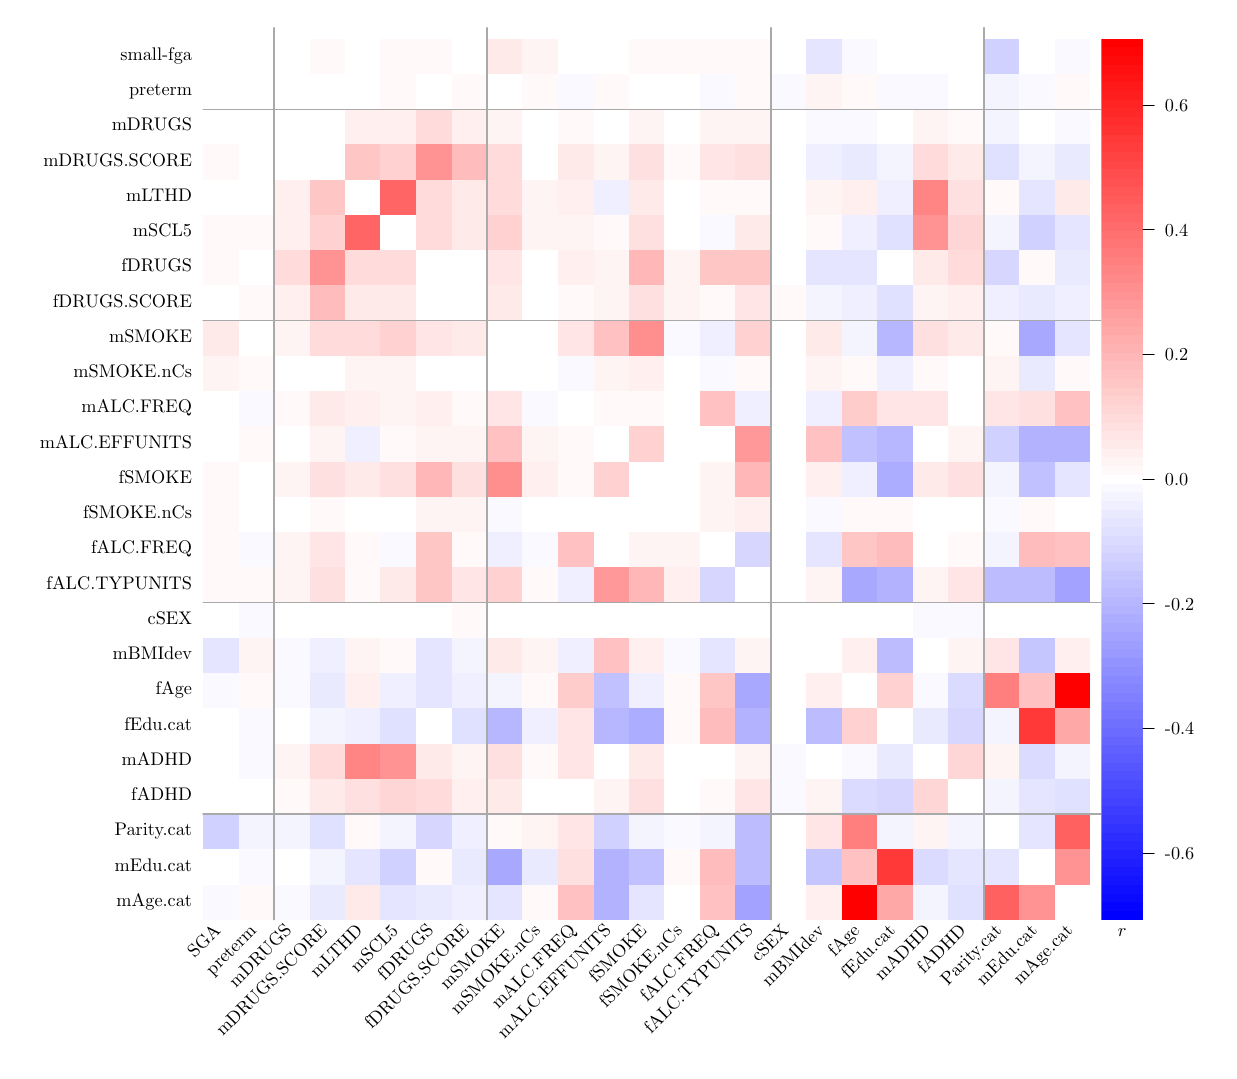
\begin{tikzpicture}[x=1pt,y=1pt]
\definecolor{fillColor}{RGB}{255,255,255}
\path[use as bounding box,fill=fillColor,fill opacity=0.00] (0,0) rectangle (426.79,369.89);
\begin{scope}
\path[clip] ( 63.36, 47.52) rectangle (384.03,365.93);
\definecolor{fillColor}{RGB}{249,249,255}

\path[fill=fillColor] ( 63.36, 47.52) rectangle ( 76.19, 60.26);
\definecolor{fillColor}{RGB}{255,255,255}

\path[fill=fillColor] ( 63.36, 60.26) rectangle ( 76.19, 72.99);
\definecolor{fillColor}{RGB}{209,209,255}

\path[fill=fillColor] ( 63.36, 72.99) rectangle ( 76.19, 85.73);
\definecolor{fillColor}{RGB}{255,255,255}

\path[fill=fillColor] ( 63.36, 85.73) rectangle ( 76.19, 98.46);

\path[fill=fillColor] ( 63.36, 98.46) rectangle ( 76.19,111.20);

\path[fill=fillColor] ( 63.36,111.20) rectangle ( 76.19,123.94);
\definecolor{fillColor}{RGB}{249,249,255}

\path[fill=fillColor] ( 63.36,123.94) rectangle ( 76.19,136.67);
\definecolor{fillColor}{RGB}{229,229,255}

\path[fill=fillColor] ( 63.36,136.67) rectangle ( 76.19,149.41);
\definecolor{fillColor}{RGB}{255,255,255}

\path[fill=fillColor] ( 63.36,149.41) rectangle ( 76.19,162.15);
\definecolor{fillColor}{RGB}{255,249,249}

\path[fill=fillColor] ( 63.36,162.15) rectangle ( 76.19,174.88);

\path[fill=fillColor] ( 63.36,174.88) rectangle ( 76.19,187.62);

\path[fill=fillColor] ( 63.36,187.62) rectangle ( 76.19,200.35);

\path[fill=fillColor] ( 63.36,200.35) rectangle ( 76.19,213.09);
\definecolor{fillColor}{RGB}{255,255,255}

\path[fill=fillColor] ( 63.36,213.09) rectangle ( 76.19,225.83);

\path[fill=fillColor] ( 63.36,225.83) rectangle ( 76.19,238.56);
\definecolor{fillColor}{RGB}{255,244,244}

\path[fill=fillColor] ( 63.36,238.56) rectangle ( 76.19,251.30);
\definecolor{fillColor}{RGB}{255,234,234}

\path[fill=fillColor] ( 63.36,251.30) rectangle ( 76.19,264.04);
\definecolor{fillColor}{RGB}{255,255,255}

\path[fill=fillColor] ( 63.36,264.04) rectangle ( 76.19,276.77);
\definecolor{fillColor}{RGB}{255,249,249}

\path[fill=fillColor] ( 63.36,276.77) rectangle ( 76.19,289.51);

\path[fill=fillColor] ( 63.36,289.51) rectangle ( 76.19,302.24);
\definecolor{fillColor}{RGB}{255,255,255}

\path[fill=fillColor] ( 63.36,302.24) rectangle ( 76.19,314.98);
\definecolor{fillColor}{RGB}{255,249,249}

\path[fill=fillColor] ( 63.36,314.98) rectangle ( 76.19,327.72);
\definecolor{fillColor}{RGB}{255,255,255}

\path[fill=fillColor] ( 63.36,327.72) rectangle ( 76.19,340.45);

\path[fill=fillColor] ( 63.36,340.45) rectangle ( 76.19,353.19);
\definecolor{fillColor}{RGB}{255,249,249}

\path[fill=fillColor] ( 76.19, 47.52) rectangle ( 89.01, 60.26);
\definecolor{fillColor}{RGB}{249,249,255}

\path[fill=fillColor] ( 76.19, 60.26) rectangle ( 89.01, 72.99);
\definecolor{fillColor}{RGB}{244,244,255}

\path[fill=fillColor] ( 76.19, 72.99) rectangle ( 89.01, 85.73);
\definecolor{fillColor}{RGB}{255,255,255}

\path[fill=fillColor] ( 76.19, 85.73) rectangle ( 89.01, 98.46);
\definecolor{fillColor}{RGB}{249,249,255}

\path[fill=fillColor] ( 76.19, 98.46) rectangle ( 89.01,111.20);

\path[fill=fillColor] ( 76.19,111.20) rectangle ( 89.01,123.94);
\definecolor{fillColor}{RGB}{255,249,249}

\path[fill=fillColor] ( 76.19,123.94) rectangle ( 89.01,136.67);
\definecolor{fillColor}{RGB}{255,244,244}

\path[fill=fillColor] ( 76.19,136.67) rectangle ( 89.01,149.41);
\definecolor{fillColor}{RGB}{249,249,255}

\path[fill=fillColor] ( 76.19,149.41) rectangle ( 89.01,162.15);
\definecolor{fillColor}{RGB}{255,249,249}

\path[fill=fillColor] ( 76.19,162.15) rectangle ( 89.01,174.88);
\definecolor{fillColor}{RGB}{249,249,255}

\path[fill=fillColor] ( 76.19,174.88) rectangle ( 89.01,187.62);
\definecolor{fillColor}{RGB}{255,255,255}

\path[fill=fillColor] ( 76.19,187.62) rectangle ( 89.01,200.35);

\path[fill=fillColor] ( 76.19,200.35) rectangle ( 89.01,213.09);
\definecolor{fillColor}{RGB}{255,249,249}

\path[fill=fillColor] ( 76.19,213.09) rectangle ( 89.01,225.83);
\definecolor{fillColor}{RGB}{249,249,255}

\path[fill=fillColor] ( 76.19,225.83) rectangle ( 89.01,238.56);
\definecolor{fillColor}{RGB}{255,249,249}

\path[fill=fillColor] ( 76.19,238.56) rectangle ( 89.01,251.30);
\definecolor{fillColor}{RGB}{255,255,255}

\path[fill=fillColor] ( 76.19,251.30) rectangle ( 89.01,264.04);
\definecolor{fillColor}{RGB}{255,249,249}

\path[fill=fillColor] ( 76.19,264.04) rectangle ( 89.01,276.77);
\definecolor{fillColor}{RGB}{255,255,255}

\path[fill=fillColor] ( 76.19,276.77) rectangle ( 89.01,289.51);
\definecolor{fillColor}{RGB}{255,249,249}

\path[fill=fillColor] ( 76.19,289.51) rectangle ( 89.01,302.24);
\definecolor{fillColor}{RGB}{255,255,255}

\path[fill=fillColor] ( 76.19,302.24) rectangle ( 89.01,314.98);

\path[fill=fillColor] ( 76.19,314.98) rectangle ( 89.01,327.72);

\path[fill=fillColor] ( 76.19,327.72) rectangle ( 89.01,340.45);

\path[fill=fillColor] ( 76.19,353.19) rectangle ( 89.01,365.93);
\definecolor{fillColor}{RGB}{249,249,255}

\path[fill=fillColor] ( 89.01, 47.52) rectangle (101.84, 60.26);
\definecolor{fillColor}{RGB}{255,255,255}

\path[fill=fillColor] ( 89.01, 60.26) rectangle (101.84, 72.99);
\definecolor{fillColor}{RGB}{244,244,255}

\path[fill=fillColor] ( 89.01, 72.99) rectangle (101.84, 85.73);
\definecolor{fillColor}{RGB}{255,249,249}

\path[fill=fillColor] ( 89.01, 85.73) rectangle (101.84, 98.46);
\definecolor{fillColor}{RGB}{255,244,244}

\path[fill=fillColor] ( 89.01, 98.46) rectangle (101.84,111.20);
\definecolor{fillColor}{RGB}{255,255,255}

\path[fill=fillColor] ( 89.01,111.20) rectangle (101.84,123.94);
\definecolor{fillColor}{RGB}{249,249,255}

\path[fill=fillColor] ( 89.01,123.94) rectangle (101.84,136.67);

\path[fill=fillColor] ( 89.01,136.67) rectangle (101.84,149.41);
\definecolor{fillColor}{RGB}{255,255,255}

\path[fill=fillColor] ( 89.01,149.41) rectangle (101.84,162.15);
\definecolor{fillColor}{RGB}{255,244,244}

\path[fill=fillColor] ( 89.01,162.15) rectangle (101.84,174.88);

\path[fill=fillColor] ( 89.01,174.88) rectangle (101.84,187.62);
\definecolor{fillColor}{RGB}{255,255,255}

\path[fill=fillColor] ( 89.01,187.62) rectangle (101.84,200.35);
\definecolor{fillColor}{RGB}{255,244,244}

\path[fill=fillColor] ( 89.01,200.35) rectangle (101.84,213.09);
\definecolor{fillColor}{RGB}{255,255,255}

\path[fill=fillColor] ( 89.01,213.09) rectangle (101.84,225.83);
\definecolor{fillColor}{RGB}{255,249,249}

\path[fill=fillColor] ( 89.01,225.83) rectangle (101.84,238.56);
\definecolor{fillColor}{RGB}{255,255,255}

\path[fill=fillColor] ( 89.01,238.56) rectangle (101.84,251.30);
\definecolor{fillColor}{RGB}{255,244,244}

\path[fill=fillColor] ( 89.01,251.30) rectangle (101.84,264.04);
\definecolor{fillColor}{RGB}{255,239,239}

\path[fill=fillColor] ( 89.01,264.04) rectangle (101.84,276.77);
\definecolor{fillColor}{RGB}{255,219,219}

\path[fill=fillColor] ( 89.01,276.77) rectangle (101.84,289.51);
\definecolor{fillColor}{RGB}{255,239,239}

\path[fill=fillColor] ( 89.01,289.51) rectangle (101.84,302.24);

\path[fill=fillColor] ( 89.01,302.24) rectangle (101.84,314.98);
\definecolor{fillColor}{RGB}{255,255,255}

\path[fill=fillColor] ( 89.01,314.98) rectangle (101.84,327.72);

\path[fill=fillColor] ( 89.01,340.45) rectangle (101.84,353.19);

\path[fill=fillColor] ( 89.01,353.19) rectangle (101.84,365.93);
\definecolor{fillColor}{RGB}{234,234,255}

\path[fill=fillColor] (101.84, 47.52) rectangle (114.67, 60.26);
\definecolor{fillColor}{RGB}{244,244,255}

\path[fill=fillColor] (101.84, 60.26) rectangle (114.67, 72.99);
\definecolor{fillColor}{RGB}{224,224,255}

\path[fill=fillColor] (101.84, 72.99) rectangle (114.67, 85.73);
\definecolor{fillColor}{RGB}{255,234,234}

\path[fill=fillColor] (101.84, 85.73) rectangle (114.67, 98.46);
\definecolor{fillColor}{RGB}{255,219,219}

\path[fill=fillColor] (101.84, 98.46) rectangle (114.67,111.20);
\definecolor{fillColor}{RGB}{244,244,255}

\path[fill=fillColor] (101.84,111.20) rectangle (114.67,123.94);
\definecolor{fillColor}{RGB}{234,234,255}

\path[fill=fillColor] (101.84,123.94) rectangle (114.67,136.67);
\definecolor{fillColor}{RGB}{239,239,255}

\path[fill=fillColor] (101.84,136.67) rectangle (114.67,149.41);
\definecolor{fillColor}{RGB}{255,255,255}

\path[fill=fillColor] (101.84,149.41) rectangle (114.67,162.15);
\definecolor{fillColor}{RGB}{255,224,224}

\path[fill=fillColor] (101.84,162.15) rectangle (114.67,174.88);
\definecolor{fillColor}{RGB}{255,229,229}

\path[fill=fillColor] (101.84,174.88) rectangle (114.67,187.62);
\definecolor{fillColor}{RGB}{255,249,249}

\path[fill=fillColor] (101.84,187.62) rectangle (114.67,200.35);
\definecolor{fillColor}{RGB}{255,224,224}

\path[fill=fillColor] (101.84,200.35) rectangle (114.67,213.09);
\definecolor{fillColor}{RGB}{255,244,244}

\path[fill=fillColor] (101.84,213.09) rectangle (114.67,225.83);
\definecolor{fillColor}{RGB}{255,234,234}

\path[fill=fillColor] (101.84,225.83) rectangle (114.67,238.56);
\definecolor{fillColor}{RGB}{255,255,255}

\path[fill=fillColor] (101.84,238.56) rectangle (114.67,251.30);
\definecolor{fillColor}{RGB}{255,219,219}

\path[fill=fillColor] (101.84,251.30) rectangle (114.67,264.04);
\definecolor{fillColor}{RGB}{255,188,188}

\path[fill=fillColor] (101.84,264.04) rectangle (114.67,276.77);
\definecolor{fillColor}{RGB}{255,147,147}

\path[fill=fillColor] (101.84,276.77) rectangle (114.67,289.51);
\definecolor{fillColor}{RGB}{255,209,209}

\path[fill=fillColor] (101.84,289.51) rectangle (114.67,302.24);
\definecolor{fillColor}{RGB}{255,198,198}

\path[fill=fillColor] (101.84,302.24) rectangle (114.67,314.98);
\definecolor{fillColor}{RGB}{255,255,255}

\path[fill=fillColor] (101.84,327.72) rectangle (114.67,340.45);

\path[fill=fillColor] (101.84,340.45) rectangle (114.67,353.19);
\definecolor{fillColor}{RGB}{255,249,249}

\path[fill=fillColor] (101.84,353.19) rectangle (114.67,365.93);
\definecolor{fillColor}{RGB}{255,234,234}

\path[fill=fillColor] (114.67, 47.52) rectangle (127.49, 60.26);
\definecolor{fillColor}{RGB}{229,229,255}

\path[fill=fillColor] (114.67, 60.26) rectangle (127.49, 72.99);
\definecolor{fillColor}{RGB}{255,249,249}

\path[fill=fillColor] (114.67, 72.99) rectangle (127.49, 85.73);
\definecolor{fillColor}{RGB}{255,224,224}

\path[fill=fillColor] (114.67, 85.73) rectangle (127.49, 98.46);
\definecolor{fillColor}{RGB}{255,132,132}

\path[fill=fillColor] (114.67, 98.46) rectangle (127.49,111.20);
\definecolor{fillColor}{RGB}{239,239,255}

\path[fill=fillColor] (114.67,111.20) rectangle (127.49,123.94);
\definecolor{fillColor}{RGB}{255,239,239}

\path[fill=fillColor] (114.67,123.94) rectangle (127.49,136.67);
\definecolor{fillColor}{RGB}{255,244,244}

\path[fill=fillColor] (114.67,136.67) rectangle (127.49,149.41);
\definecolor{fillColor}{RGB}{255,255,255}

\path[fill=fillColor] (114.67,149.41) rectangle (127.49,162.15);
\definecolor{fillColor}{RGB}{255,249,249}

\path[fill=fillColor] (114.67,162.15) rectangle (127.49,174.88);

\path[fill=fillColor] (114.67,174.88) rectangle (127.49,187.62);
\definecolor{fillColor}{RGB}{255,255,255}

\path[fill=fillColor] (114.67,187.62) rectangle (127.49,200.35);
\definecolor{fillColor}{RGB}{255,234,234}

\path[fill=fillColor] (114.67,200.35) rectangle (127.49,213.09);
\definecolor{fillColor}{RGB}{239,239,255}

\path[fill=fillColor] (114.67,213.09) rectangle (127.49,225.83);
\definecolor{fillColor}{RGB}{255,239,239}

\path[fill=fillColor] (114.67,225.83) rectangle (127.49,238.56);
\definecolor{fillColor}{RGB}{255,244,244}

\path[fill=fillColor] (114.67,238.56) rectangle (127.49,251.30);
\definecolor{fillColor}{RGB}{255,219,219}

\path[fill=fillColor] (114.67,251.30) rectangle (127.49,264.04);
\definecolor{fillColor}{RGB}{255,234,234}

\path[fill=fillColor] (114.67,264.04) rectangle (127.49,276.77);
\definecolor{fillColor}{RGB}{255,219,219}

\path[fill=fillColor] (114.67,276.77) rectangle (127.49,289.51);
\definecolor{fillColor}{RGB}{255,101,101}

\path[fill=fillColor] (114.67,289.51) rectangle (127.49,302.24);
\definecolor{fillColor}{RGB}{255,198,198}

\path[fill=fillColor] (114.67,314.98) rectangle (127.49,327.72);
\definecolor{fillColor}{RGB}{255,239,239}

\path[fill=fillColor] (114.67,327.72) rectangle (127.49,340.45);
\definecolor{fillColor}{RGB}{255,255,255}

\path[fill=fillColor] (114.67,340.45) rectangle (127.49,353.19);

\path[fill=fillColor] (114.67,353.19) rectangle (127.49,365.93);
\definecolor{fillColor}{RGB}{229,229,255}

\path[fill=fillColor] (127.49, 47.52) rectangle (140.32, 60.26);
\definecolor{fillColor}{RGB}{209,209,255}

\path[fill=fillColor] (127.49, 60.26) rectangle (140.32, 72.99);
\definecolor{fillColor}{RGB}{244,244,255}

\path[fill=fillColor] (127.49, 72.99) rectangle (140.32, 85.73);
\definecolor{fillColor}{RGB}{255,214,214}

\path[fill=fillColor] (127.49, 85.73) rectangle (140.32, 98.46);
\definecolor{fillColor}{RGB}{255,147,147}

\path[fill=fillColor] (127.49, 98.46) rectangle (140.32,111.20);
\definecolor{fillColor}{RGB}{224,224,255}

\path[fill=fillColor] (127.49,111.20) rectangle (140.32,123.94);
\definecolor{fillColor}{RGB}{239,239,255}

\path[fill=fillColor] (127.49,123.94) rectangle (140.32,136.67);
\definecolor{fillColor}{RGB}{255,249,249}

\path[fill=fillColor] (127.49,136.67) rectangle (140.32,149.41);
\definecolor{fillColor}{RGB}{255,255,255}

\path[fill=fillColor] (127.49,149.41) rectangle (140.32,162.15);
\definecolor{fillColor}{RGB}{255,234,234}

\path[fill=fillColor] (127.49,162.15) rectangle (140.32,174.88);
\definecolor{fillColor}{RGB}{249,249,255}

\path[fill=fillColor] (127.49,174.88) rectangle (140.32,187.62);
\definecolor{fillColor}{RGB}{255,255,255}

\path[fill=fillColor] (127.49,187.62) rectangle (140.32,200.35);
\definecolor{fillColor}{RGB}{255,224,224}

\path[fill=fillColor] (127.49,200.35) rectangle (140.32,213.09);
\definecolor{fillColor}{RGB}{255,249,249}

\path[fill=fillColor] (127.49,213.09) rectangle (140.32,225.83);
\definecolor{fillColor}{RGB}{255,244,244}

\path[fill=fillColor] (127.49,225.83) rectangle (140.32,238.56);

\path[fill=fillColor] (127.49,238.56) rectangle (140.32,251.30);
\definecolor{fillColor}{RGB}{255,209,209}

\path[fill=fillColor] (127.49,251.30) rectangle (140.32,264.04);
\definecolor{fillColor}{RGB}{255,234,234}

\path[fill=fillColor] (127.49,264.04) rectangle (140.32,276.77);
\definecolor{fillColor}{RGB}{255,219,219}

\path[fill=fillColor] (127.49,276.77) rectangle (140.32,289.51);
\definecolor{fillColor}{RGB}{255,101,101}

\path[fill=fillColor] (127.49,302.24) rectangle (140.32,314.98);
\definecolor{fillColor}{RGB}{255,209,209}

\path[fill=fillColor] (127.49,314.98) rectangle (140.32,327.72);
\definecolor{fillColor}{RGB}{255,239,239}

\path[fill=fillColor] (127.49,327.72) rectangle (140.32,340.45);
\definecolor{fillColor}{RGB}{255,249,249}

\path[fill=fillColor] (127.49,340.45) rectangle (140.32,353.19);

\path[fill=fillColor] (127.49,353.19) rectangle (140.32,365.93);
\definecolor{fillColor}{RGB}{234,234,255}

\path[fill=fillColor] (140.32, 47.52) rectangle (153.15, 60.26);
\definecolor{fillColor}{RGB}{255,249,249}

\path[fill=fillColor] (140.32, 60.26) rectangle (153.15, 72.99);
\definecolor{fillColor}{RGB}{214,214,255}

\path[fill=fillColor] (140.32, 72.99) rectangle (153.15, 85.73);
\definecolor{fillColor}{RGB}{255,219,219}

\path[fill=fillColor] (140.32, 85.73) rectangle (153.15, 98.46);
\definecolor{fillColor}{RGB}{255,234,234}

\path[fill=fillColor] (140.32, 98.46) rectangle (153.15,111.20);
\definecolor{fillColor}{RGB}{255,255,255}

\path[fill=fillColor] (140.32,111.20) rectangle (153.15,123.94);
\definecolor{fillColor}{RGB}{229,229,255}

\path[fill=fillColor] (140.32,123.94) rectangle (153.15,136.67);

\path[fill=fillColor] (140.32,136.67) rectangle (153.15,149.41);
\definecolor{fillColor}{RGB}{255,255,255}

\path[fill=fillColor] (140.32,149.41) rectangle (153.15,162.15);
\definecolor{fillColor}{RGB}{255,198,198}

\path[fill=fillColor] (140.32,162.15) rectangle (153.15,174.88);

\path[fill=fillColor] (140.32,174.88) rectangle (153.15,187.62);
\definecolor{fillColor}{RGB}{255,244,244}

\path[fill=fillColor] (140.32,187.62) rectangle (153.15,200.35);
\definecolor{fillColor}{RGB}{255,183,183}

\path[fill=fillColor] (140.32,200.35) rectangle (153.15,213.09);
\definecolor{fillColor}{RGB}{255,244,244}

\path[fill=fillColor] (140.32,213.09) rectangle (153.15,225.83);
\definecolor{fillColor}{RGB}{255,239,239}

\path[fill=fillColor] (140.32,225.83) rectangle (153.15,238.56);
\definecolor{fillColor}{RGB}{255,255,255}

\path[fill=fillColor] (140.32,238.56) rectangle (153.15,251.30);
\definecolor{fillColor}{RGB}{255,229,229}

\path[fill=fillColor] (140.32,251.30) rectangle (153.15,264.04);
\definecolor{fillColor}{RGB}{255,255,255}

\path[fill=fillColor] (140.32,264.04) rectangle (153.15,276.77);
\definecolor{fillColor}{RGB}{255,219,219}

\path[fill=fillColor] (140.32,289.51) rectangle (153.15,302.24);

\path[fill=fillColor] (140.32,302.24) rectangle (153.15,314.98);
\definecolor{fillColor}{RGB}{255,147,147}

\path[fill=fillColor] (140.32,314.98) rectangle (153.15,327.72);
\definecolor{fillColor}{RGB}{255,219,219}

\path[fill=fillColor] (140.32,327.72) rectangle (153.15,340.45);
\definecolor{fillColor}{RGB}{255,255,255}

\path[fill=fillColor] (140.32,340.45) rectangle (153.15,353.19);
\definecolor{fillColor}{RGB}{255,249,249}

\path[fill=fillColor] (140.32,353.19) rectangle (153.15,365.93);
\definecolor{fillColor}{RGB}{239,239,255}

\path[fill=fillColor] (153.15, 47.52) rectangle (165.98, 60.26);
\definecolor{fillColor}{RGB}{234,234,255}

\path[fill=fillColor] (153.15, 60.26) rectangle (165.98, 72.99);
\definecolor{fillColor}{RGB}{239,239,255}

\path[fill=fillColor] (153.15, 72.99) rectangle (165.98, 85.73);
\definecolor{fillColor}{RGB}{255,239,239}

\path[fill=fillColor] (153.15, 85.73) rectangle (165.98, 98.46);
\definecolor{fillColor}{RGB}{255,244,244}

\path[fill=fillColor] (153.15, 98.46) rectangle (165.98,111.20);
\definecolor{fillColor}{RGB}{224,224,255}

\path[fill=fillColor] (153.15,111.20) rectangle (165.98,123.94);
\definecolor{fillColor}{RGB}{239,239,255}

\path[fill=fillColor] (153.15,123.94) rectangle (165.98,136.67);
\definecolor{fillColor}{RGB}{244,244,255}

\path[fill=fillColor] (153.15,136.67) rectangle (165.98,149.41);
\definecolor{fillColor}{RGB}{255,249,249}

\path[fill=fillColor] (153.15,149.41) rectangle (165.98,162.15);
\definecolor{fillColor}{RGB}{255,229,229}

\path[fill=fillColor] (153.15,162.15) rectangle (165.98,174.88);
\definecolor{fillColor}{RGB}{255,249,249}

\path[fill=fillColor] (153.15,174.88) rectangle (165.98,187.62);
\definecolor{fillColor}{RGB}{255,244,244}

\path[fill=fillColor] (153.15,187.62) rectangle (165.98,200.35);
\definecolor{fillColor}{RGB}{255,224,224}

\path[fill=fillColor] (153.15,200.35) rectangle (165.98,213.09);
\definecolor{fillColor}{RGB}{255,244,244}

\path[fill=fillColor] (153.15,213.09) rectangle (165.98,225.83);
\definecolor{fillColor}{RGB}{255,249,249}

\path[fill=fillColor] (153.15,225.83) rectangle (165.98,238.56);
\definecolor{fillColor}{RGB}{255,255,255}

\path[fill=fillColor] (153.15,238.56) rectangle (165.98,251.30);
\definecolor{fillColor}{RGB}{255,234,234}

\path[fill=fillColor] (153.15,251.30) rectangle (165.98,264.04);
\definecolor{fillColor}{RGB}{255,255,255}

\path[fill=fillColor] (153.15,276.77) rectangle (165.98,289.51);
\definecolor{fillColor}{RGB}{255,234,234}

\path[fill=fillColor] (153.15,289.51) rectangle (165.98,302.24);

\path[fill=fillColor] (153.15,302.24) rectangle (165.98,314.98);
\definecolor{fillColor}{RGB}{255,188,188}

\path[fill=fillColor] (153.15,314.98) rectangle (165.98,327.72);
\definecolor{fillColor}{RGB}{255,239,239}

\path[fill=fillColor] (153.15,327.72) rectangle (165.98,340.45);
\definecolor{fillColor}{RGB}{255,249,249}

\path[fill=fillColor] (153.15,340.45) rectangle (165.98,353.19);
\definecolor{fillColor}{RGB}{255,255,255}

\path[fill=fillColor] (153.15,353.19) rectangle (165.98,365.93);
\definecolor{fillColor}{RGB}{229,229,255}

\path[fill=fillColor] (165.98, 47.52) rectangle (178.80, 60.26);
\definecolor{fillColor}{RGB}{168,168,255}

\path[fill=fillColor] (165.98, 60.26) rectangle (178.80, 72.99);
\definecolor{fillColor}{RGB}{255,249,249}

\path[fill=fillColor] (165.98, 72.99) rectangle (178.80, 85.73);
\definecolor{fillColor}{RGB}{255,234,234}

\path[fill=fillColor] (165.98, 85.73) rectangle (178.80, 98.46);
\definecolor{fillColor}{RGB}{255,224,224}

\path[fill=fillColor] (165.98, 98.46) rectangle (178.80,111.20);
\definecolor{fillColor}{RGB}{183,183,255}

\path[fill=fillColor] (165.98,111.20) rectangle (178.80,123.94);
\definecolor{fillColor}{RGB}{244,244,255}

\path[fill=fillColor] (165.98,123.94) rectangle (178.80,136.67);
\definecolor{fillColor}{RGB}{255,234,234}

\path[fill=fillColor] (165.98,136.67) rectangle (178.80,149.41);
\definecolor{fillColor}{RGB}{255,255,255}

\path[fill=fillColor] (165.98,149.41) rectangle (178.80,162.15);
\definecolor{fillColor}{RGB}{255,209,209}

\path[fill=fillColor] (165.98,162.15) rectangle (178.80,174.88);
\definecolor{fillColor}{RGB}{239,239,255}

\path[fill=fillColor] (165.98,174.88) rectangle (178.80,187.62);
\definecolor{fillColor}{RGB}{249,249,255}

\path[fill=fillColor] (165.98,187.62) rectangle (178.80,200.35);
\definecolor{fillColor}{RGB}{255,142,142}

\path[fill=fillColor] (165.98,200.35) rectangle (178.80,213.09);
\definecolor{fillColor}{RGB}{255,193,193}

\path[fill=fillColor] (165.98,213.09) rectangle (178.80,225.83);
\definecolor{fillColor}{RGB}{255,229,229}

\path[fill=fillColor] (165.98,225.83) rectangle (178.80,238.56);
\definecolor{fillColor}{RGB}{255,255,255}

\path[fill=fillColor] (165.98,238.56) rectangle (178.80,251.30);
\definecolor{fillColor}{RGB}{255,234,234}

\path[fill=fillColor] (165.98,264.04) rectangle (178.80,276.77);
\definecolor{fillColor}{RGB}{255,229,229}

\path[fill=fillColor] (165.98,276.77) rectangle (178.80,289.51);
\definecolor{fillColor}{RGB}{255,209,209}

\path[fill=fillColor] (165.98,289.51) rectangle (178.80,302.24);
\definecolor{fillColor}{RGB}{255,219,219}

\path[fill=fillColor] (165.98,302.24) rectangle (178.80,314.98);

\path[fill=fillColor] (165.98,314.98) rectangle (178.80,327.72);
\definecolor{fillColor}{RGB}{255,244,244}

\path[fill=fillColor] (165.98,327.72) rectangle (178.80,340.45);
\definecolor{fillColor}{RGB}{255,255,255}

\path[fill=fillColor] (165.98,340.45) rectangle (178.80,353.19);
\definecolor{fillColor}{RGB}{255,234,234}

\path[fill=fillColor] (165.98,353.19) rectangle (178.80,365.93);
\definecolor{fillColor}{RGB}{255,249,249}

\path[fill=fillColor] (178.80, 47.52) rectangle (191.63, 60.26);
\definecolor{fillColor}{RGB}{234,234,255}

\path[fill=fillColor] (178.80, 60.26) rectangle (191.63, 72.99);
\definecolor{fillColor}{RGB}{255,244,244}

\path[fill=fillColor] (178.80, 72.99) rectangle (191.63, 85.73);
\definecolor{fillColor}{RGB}{255,255,255}

\path[fill=fillColor] (178.80, 85.73) rectangle (191.63, 98.46);
\definecolor{fillColor}{RGB}{255,249,249}

\path[fill=fillColor] (178.80, 98.46) rectangle (191.63,111.20);
\definecolor{fillColor}{RGB}{239,239,255}

\path[fill=fillColor] (178.80,111.20) rectangle (191.63,123.94);
\definecolor{fillColor}{RGB}{255,249,249}

\path[fill=fillColor] (178.80,123.94) rectangle (191.63,136.67);
\definecolor{fillColor}{RGB}{255,244,244}

\path[fill=fillColor] (178.80,136.67) rectangle (191.63,149.41);
\definecolor{fillColor}{RGB}{255,255,255}

\path[fill=fillColor] (178.80,149.41) rectangle (191.63,162.15);
\definecolor{fillColor}{RGB}{255,249,249}

\path[fill=fillColor] (178.80,162.15) rectangle (191.63,174.88);
\definecolor{fillColor}{RGB}{249,249,255}

\path[fill=fillColor] (178.80,174.88) rectangle (191.63,187.62);
\definecolor{fillColor}{RGB}{255,255,255}

\path[fill=fillColor] (178.80,187.62) rectangle (191.63,200.35);
\definecolor{fillColor}{RGB}{255,239,239}

\path[fill=fillColor] (178.80,200.35) rectangle (191.63,213.09);
\definecolor{fillColor}{RGB}{255,244,244}

\path[fill=fillColor] (178.80,213.09) rectangle (191.63,225.83);
\definecolor{fillColor}{RGB}{249,249,255}

\path[fill=fillColor] (178.80,225.83) rectangle (191.63,238.56);
\definecolor{fillColor}{RGB}{255,255,255}

\path[fill=fillColor] (178.80,251.30) rectangle (191.63,264.04);

\path[fill=fillColor] (178.80,264.04) rectangle (191.63,276.77);

\path[fill=fillColor] (178.80,276.77) rectangle (191.63,289.51);
\definecolor{fillColor}{RGB}{255,244,244}

\path[fill=fillColor] (178.80,289.51) rectangle (191.63,302.24);

\path[fill=fillColor] (178.80,302.24) rectangle (191.63,314.98);
\definecolor{fillColor}{RGB}{255,255,255}

\path[fill=fillColor] (178.80,314.98) rectangle (191.63,327.72);

\path[fill=fillColor] (178.80,327.72) rectangle (191.63,340.45);
\definecolor{fillColor}{RGB}{255,249,249}

\path[fill=fillColor] (178.80,340.45) rectangle (191.63,353.19);
\definecolor{fillColor}{RGB}{255,244,244}

\path[fill=fillColor] (178.80,353.19) rectangle (191.63,365.93);
\definecolor{fillColor}{RGB}{255,193,193}

\path[fill=fillColor] (191.63, 47.52) rectangle (204.46, 60.26);
\definecolor{fillColor}{RGB}{255,224,224}

\path[fill=fillColor] (191.63, 60.26) rectangle (204.46, 72.99);
\definecolor{fillColor}{RGB}{255,229,229}

\path[fill=fillColor] (191.63, 72.99) rectangle (204.46, 85.73);
\definecolor{fillColor}{RGB}{255,255,255}

\path[fill=fillColor] (191.63, 85.73) rectangle (204.46, 98.46);
\definecolor{fillColor}{RGB}{255,229,229}

\path[fill=fillColor] (191.63, 98.46) rectangle (204.46,111.20);

\path[fill=fillColor] (191.63,111.20) rectangle (204.46,123.94);
\definecolor{fillColor}{RGB}{255,204,204}

\path[fill=fillColor] (191.63,123.94) rectangle (204.46,136.67);
\definecolor{fillColor}{RGB}{239,239,255}

\path[fill=fillColor] (191.63,136.67) rectangle (204.46,149.41);
\definecolor{fillColor}{RGB}{255,255,255}

\path[fill=fillColor] (191.63,149.41) rectangle (204.46,162.15);
\definecolor{fillColor}{RGB}{239,239,255}

\path[fill=fillColor] (191.63,162.15) rectangle (204.46,174.88);
\definecolor{fillColor}{RGB}{255,193,193}

\path[fill=fillColor] (191.63,174.88) rectangle (204.46,187.62);
\definecolor{fillColor}{RGB}{255,255,255}

\path[fill=fillColor] (191.63,187.62) rectangle (204.46,200.35);
\definecolor{fillColor}{RGB}{255,249,249}

\path[fill=fillColor] (191.63,200.35) rectangle (204.46,213.09);

\path[fill=fillColor] (191.63,213.09) rectangle (204.46,225.83);
\definecolor{fillColor}{RGB}{249,249,255}

\path[fill=fillColor] (191.63,238.56) rectangle (204.46,251.30);
\definecolor{fillColor}{RGB}{255,229,229}

\path[fill=fillColor] (191.63,251.30) rectangle (204.46,264.04);
\definecolor{fillColor}{RGB}{255,249,249}

\path[fill=fillColor] (191.63,264.04) rectangle (204.46,276.77);
\definecolor{fillColor}{RGB}{255,239,239}

\path[fill=fillColor] (191.63,276.77) rectangle (204.46,289.51);
\definecolor{fillColor}{RGB}{255,244,244}

\path[fill=fillColor] (191.63,289.51) rectangle (204.46,302.24);
\definecolor{fillColor}{RGB}{255,239,239}

\path[fill=fillColor] (191.63,302.24) rectangle (204.46,314.98);
\definecolor{fillColor}{RGB}{255,234,234}

\path[fill=fillColor] (191.63,314.98) rectangle (204.46,327.72);
\definecolor{fillColor}{RGB}{255,249,249}

\path[fill=fillColor] (191.63,327.72) rectangle (204.46,340.45);
\definecolor{fillColor}{RGB}{249,249,255}

\path[fill=fillColor] (191.63,340.45) rectangle (204.46,353.19);
\definecolor{fillColor}{RGB}{255,255,255}

\path[fill=fillColor] (191.63,353.19) rectangle (204.46,365.93);
\definecolor{fillColor}{RGB}{178,178,255}

\path[fill=fillColor] (204.46, 47.52) rectangle (217.28, 60.26);

\path[fill=fillColor] (204.46, 60.26) rectangle (217.28, 72.99);
\definecolor{fillColor}{RGB}{209,209,255}

\path[fill=fillColor] (204.46, 72.99) rectangle (217.28, 85.73);
\definecolor{fillColor}{RGB}{255,244,244}

\path[fill=fillColor] (204.46, 85.73) rectangle (217.28, 98.46);
\definecolor{fillColor}{RGB}{255,255,255}

\path[fill=fillColor] (204.46, 98.46) rectangle (217.28,111.20);
\definecolor{fillColor}{RGB}{183,183,255}

\path[fill=fillColor] (204.46,111.20) rectangle (217.28,123.94);
\definecolor{fillColor}{RGB}{193,193,255}

\path[fill=fillColor] (204.46,123.94) rectangle (217.28,136.67);
\definecolor{fillColor}{RGB}{255,193,193}

\path[fill=fillColor] (204.46,136.67) rectangle (217.28,149.41);
\definecolor{fillColor}{RGB}{255,255,255}

\path[fill=fillColor] (204.46,149.41) rectangle (217.28,162.15);
\definecolor{fillColor}{RGB}{255,152,152}

\path[fill=fillColor] (204.46,162.15) rectangle (217.28,174.88);
\definecolor{fillColor}{RGB}{255,255,255}

\path[fill=fillColor] (204.46,174.88) rectangle (217.28,187.62);

\path[fill=fillColor] (204.46,187.62) rectangle (217.28,200.35);
\definecolor{fillColor}{RGB}{255,209,209}

\path[fill=fillColor] (204.46,200.35) rectangle (217.28,213.09);
\definecolor{fillColor}{RGB}{255,249,249}

\path[fill=fillColor] (204.46,225.83) rectangle (217.28,238.56);
\definecolor{fillColor}{RGB}{255,244,244}

\path[fill=fillColor] (204.46,238.56) rectangle (217.28,251.30);
\definecolor{fillColor}{RGB}{255,193,193}

\path[fill=fillColor] (204.46,251.30) rectangle (217.28,264.04);
\definecolor{fillColor}{RGB}{255,244,244}

\path[fill=fillColor] (204.46,264.04) rectangle (217.28,276.77);

\path[fill=fillColor] (204.46,276.77) rectangle (217.28,289.51);
\definecolor{fillColor}{RGB}{255,249,249}

\path[fill=fillColor] (204.46,289.51) rectangle (217.28,302.24);
\definecolor{fillColor}{RGB}{239,239,255}

\path[fill=fillColor] (204.46,302.24) rectangle (217.28,314.98);
\definecolor{fillColor}{RGB}{255,244,244}

\path[fill=fillColor] (204.46,314.98) rectangle (217.28,327.72);
\definecolor{fillColor}{RGB}{255,255,255}

\path[fill=fillColor] (204.46,327.72) rectangle (217.28,340.45);
\definecolor{fillColor}{RGB}{255,249,249}

\path[fill=fillColor] (204.46,340.45) rectangle (217.28,353.19);
\definecolor{fillColor}{RGB}{255,255,255}

\path[fill=fillColor] (204.46,353.19) rectangle (217.28,365.93);
\definecolor{fillColor}{RGB}{229,229,255}

\path[fill=fillColor] (217.28, 47.52) rectangle (230.11, 60.26);
\definecolor{fillColor}{RGB}{193,193,255}

\path[fill=fillColor] (217.28, 60.26) rectangle (230.11, 72.99);
\definecolor{fillColor}{RGB}{244,244,255}

\path[fill=fillColor] (217.28, 72.99) rectangle (230.11, 85.73);
\definecolor{fillColor}{RGB}{255,224,224}

\path[fill=fillColor] (217.28, 85.73) rectangle (230.11, 98.46);
\definecolor{fillColor}{RGB}{255,234,234}

\path[fill=fillColor] (217.28, 98.46) rectangle (230.11,111.20);
\definecolor{fillColor}{RGB}{173,173,255}

\path[fill=fillColor] (217.28,111.20) rectangle (230.11,123.94);
\definecolor{fillColor}{RGB}{239,239,255}

\path[fill=fillColor] (217.28,123.94) rectangle (230.11,136.67);
\definecolor{fillColor}{RGB}{255,239,239}

\path[fill=fillColor] (217.28,136.67) rectangle (230.11,149.41);
\definecolor{fillColor}{RGB}{255,255,255}

\path[fill=fillColor] (217.28,149.41) rectangle (230.11,162.15);
\definecolor{fillColor}{RGB}{255,183,183}

\path[fill=fillColor] (217.28,162.15) rectangle (230.11,174.88);
\definecolor{fillColor}{RGB}{255,244,244}

\path[fill=fillColor] (217.28,174.88) rectangle (230.11,187.62);
\definecolor{fillColor}{RGB}{255,255,255}

\path[fill=fillColor] (217.28,187.62) rectangle (230.11,200.35);
\definecolor{fillColor}{RGB}{255,209,209}

\path[fill=fillColor] (217.28,213.09) rectangle (230.11,225.83);
\definecolor{fillColor}{RGB}{255,249,249}

\path[fill=fillColor] (217.28,225.83) rectangle (230.11,238.56);
\definecolor{fillColor}{RGB}{255,239,239}

\path[fill=fillColor] (217.28,238.56) rectangle (230.11,251.30);
\definecolor{fillColor}{RGB}{255,142,142}

\path[fill=fillColor] (217.28,251.30) rectangle (230.11,264.04);
\definecolor{fillColor}{RGB}{255,224,224}

\path[fill=fillColor] (217.28,264.04) rectangle (230.11,276.77);
\definecolor{fillColor}{RGB}{255,183,183}

\path[fill=fillColor] (217.28,276.77) rectangle (230.11,289.51);
\definecolor{fillColor}{RGB}{255,224,224}

\path[fill=fillColor] (217.28,289.51) rectangle (230.11,302.24);
\definecolor{fillColor}{RGB}{255,234,234}

\path[fill=fillColor] (217.28,302.24) rectangle (230.11,314.98);
\definecolor{fillColor}{RGB}{255,224,224}

\path[fill=fillColor] (217.28,314.98) rectangle (230.11,327.72);
\definecolor{fillColor}{RGB}{255,244,244}

\path[fill=fillColor] (217.28,327.72) rectangle (230.11,340.45);
\definecolor{fillColor}{RGB}{255,255,255}

\path[fill=fillColor] (217.28,340.45) rectangle (230.11,353.19);
\definecolor{fillColor}{RGB}{255,249,249}

\path[fill=fillColor] (217.28,353.19) rectangle (230.11,365.93);
\definecolor{fillColor}{RGB}{255,255,255}

\path[fill=fillColor] (230.11, 47.52) rectangle (242.94, 60.26);
\definecolor{fillColor}{RGB}{255,249,249}

\path[fill=fillColor] (230.11, 60.26) rectangle (242.94, 72.99);
\definecolor{fillColor}{RGB}{249,249,255}

\path[fill=fillColor] (230.11, 72.99) rectangle (242.94, 85.73);
\definecolor{fillColor}{RGB}{255,255,255}

\path[fill=fillColor] (230.11, 85.73) rectangle (242.94, 98.46);

\path[fill=fillColor] (230.11, 98.46) rectangle (242.94,111.20);
\definecolor{fillColor}{RGB}{255,249,249}

\path[fill=fillColor] (230.11,111.20) rectangle (242.94,123.94);

\path[fill=fillColor] (230.11,123.94) rectangle (242.94,136.67);
\definecolor{fillColor}{RGB}{249,249,255}

\path[fill=fillColor] (230.11,136.67) rectangle (242.94,149.41);
\definecolor{fillColor}{RGB}{255,255,255}

\path[fill=fillColor] (230.11,149.41) rectangle (242.94,162.15);
\definecolor{fillColor}{RGB}{255,239,239}

\path[fill=fillColor] (230.11,162.15) rectangle (242.94,174.88);
\definecolor{fillColor}{RGB}{255,244,244}

\path[fill=fillColor] (230.11,174.88) rectangle (242.94,187.62);
\definecolor{fillColor}{RGB}{255,255,255}

\path[fill=fillColor] (230.11,200.35) rectangle (242.94,213.09);

\path[fill=fillColor] (230.11,213.09) rectangle (242.94,225.83);

\path[fill=fillColor] (230.11,225.83) rectangle (242.94,238.56);

\path[fill=fillColor] (230.11,238.56) rectangle (242.94,251.30);
\definecolor{fillColor}{RGB}{249,249,255}

\path[fill=fillColor] (230.11,251.30) rectangle (242.94,264.04);
\definecolor{fillColor}{RGB}{255,244,244}

\path[fill=fillColor] (230.11,264.04) rectangle (242.94,276.77);

\path[fill=fillColor] (230.11,276.77) rectangle (242.94,289.51);
\definecolor{fillColor}{RGB}{255,255,255}

\path[fill=fillColor] (230.11,289.51) rectangle (242.94,302.24);

\path[fill=fillColor] (230.11,302.24) rectangle (242.94,314.98);
\definecolor{fillColor}{RGB}{255,249,249}

\path[fill=fillColor] (230.11,314.98) rectangle (242.94,327.72);
\definecolor{fillColor}{RGB}{255,255,255}

\path[fill=fillColor] (230.11,327.72) rectangle (242.94,340.45);

\path[fill=fillColor] (230.11,340.45) rectangle (242.94,353.19);
\definecolor{fillColor}{RGB}{255,249,249}

\path[fill=fillColor] (230.11,353.19) rectangle (242.94,365.93);
\definecolor{fillColor}{RGB}{255,193,193}

\path[fill=fillColor] (242.94, 47.52) rectangle (255.76, 60.26);
\definecolor{fillColor}{RGB}{255,188,188}

\path[fill=fillColor] (242.94, 60.26) rectangle (255.76, 72.99);
\definecolor{fillColor}{RGB}{244,244,255}

\path[fill=fillColor] (242.94, 72.99) rectangle (255.76, 85.73);
\definecolor{fillColor}{RGB}{255,249,249}

\path[fill=fillColor] (242.94, 85.73) rectangle (255.76, 98.46);
\definecolor{fillColor}{RGB}{255,255,255}

\path[fill=fillColor] (242.94, 98.46) rectangle (255.76,111.20);
\definecolor{fillColor}{RGB}{255,188,188}

\path[fill=fillColor] (242.94,111.20) rectangle (255.76,123.94);
\definecolor{fillColor}{RGB}{255,198,198}

\path[fill=fillColor] (242.94,123.94) rectangle (255.76,136.67);
\definecolor{fillColor}{RGB}{229,229,255}

\path[fill=fillColor] (242.94,136.67) rectangle (255.76,149.41);
\definecolor{fillColor}{RGB}{255,255,255}

\path[fill=fillColor] (242.94,149.41) rectangle (255.76,162.15);
\definecolor{fillColor}{RGB}{214,214,255}

\path[fill=fillColor] (242.94,162.15) rectangle (255.76,174.88);
\definecolor{fillColor}{RGB}{255,244,244}

\path[fill=fillColor] (242.94,187.62) rectangle (255.76,200.35);

\path[fill=fillColor] (242.94,200.35) rectangle (255.76,213.09);
\definecolor{fillColor}{RGB}{255,255,255}

\path[fill=fillColor] (242.94,213.09) rectangle (255.76,225.83);
\definecolor{fillColor}{RGB}{255,193,193}

\path[fill=fillColor] (242.94,225.83) rectangle (255.76,238.56);
\definecolor{fillColor}{RGB}{249,249,255}

\path[fill=fillColor] (242.94,238.56) rectangle (255.76,251.30);
\definecolor{fillColor}{RGB}{239,239,255}

\path[fill=fillColor] (242.94,251.30) rectangle (255.76,264.04);
\definecolor{fillColor}{RGB}{255,249,249}

\path[fill=fillColor] (242.94,264.04) rectangle (255.76,276.77);
\definecolor{fillColor}{RGB}{255,198,198}

\path[fill=fillColor] (242.94,276.77) rectangle (255.76,289.51);
\definecolor{fillColor}{RGB}{249,249,255}

\path[fill=fillColor] (242.94,289.51) rectangle (255.76,302.24);
\definecolor{fillColor}{RGB}{255,249,249}

\path[fill=fillColor] (242.94,302.24) rectangle (255.76,314.98);
\definecolor{fillColor}{RGB}{255,229,229}

\path[fill=fillColor] (242.94,314.98) rectangle (255.76,327.72);
\definecolor{fillColor}{RGB}{255,244,244}

\path[fill=fillColor] (242.94,327.72) rectangle (255.76,340.45);
\definecolor{fillColor}{RGB}{249,249,255}

\path[fill=fillColor] (242.94,340.45) rectangle (255.76,353.19);
\definecolor{fillColor}{RGB}{255,249,249}

\path[fill=fillColor] (242.94,353.19) rectangle (255.76,365.93);
\definecolor{fillColor}{RGB}{163,163,255}

\path[fill=fillColor] (255.76, 47.52) rectangle (268.59, 60.26);
\definecolor{fillColor}{RGB}{188,188,255}

\path[fill=fillColor] (255.76, 60.26) rectangle (268.59, 72.99);

\path[fill=fillColor] (255.76, 72.99) rectangle (268.59, 85.73);
\definecolor{fillColor}{RGB}{255,229,229}

\path[fill=fillColor] (255.76, 85.73) rectangle (268.59, 98.46);
\definecolor{fillColor}{RGB}{255,244,244}

\path[fill=fillColor] (255.76, 98.46) rectangle (268.59,111.20);
\definecolor{fillColor}{RGB}{178,178,255}

\path[fill=fillColor] (255.76,111.20) rectangle (268.59,123.94);
\definecolor{fillColor}{RGB}{168,168,255}

\path[fill=fillColor] (255.76,123.94) rectangle (268.59,136.67);
\definecolor{fillColor}{RGB}{255,244,244}

\path[fill=fillColor] (255.76,136.67) rectangle (268.59,149.41);
\definecolor{fillColor}{RGB}{255,255,255}

\path[fill=fillColor] (255.76,149.41) rectangle (268.59,162.15);
\definecolor{fillColor}{RGB}{214,214,255}

\path[fill=fillColor] (255.76,174.88) rectangle (268.59,187.62);
\definecolor{fillColor}{RGB}{255,239,239}

\path[fill=fillColor] (255.76,187.62) rectangle (268.59,200.35);
\definecolor{fillColor}{RGB}{255,183,183}

\path[fill=fillColor] (255.76,200.35) rectangle (268.59,213.09);
\definecolor{fillColor}{RGB}{255,152,152}

\path[fill=fillColor] (255.76,213.09) rectangle (268.59,225.83);
\definecolor{fillColor}{RGB}{239,239,255}

\path[fill=fillColor] (255.76,225.83) rectangle (268.59,238.56);
\definecolor{fillColor}{RGB}{255,249,249}

\path[fill=fillColor] (255.76,238.56) rectangle (268.59,251.30);
\definecolor{fillColor}{RGB}{255,209,209}

\path[fill=fillColor] (255.76,251.30) rectangle (268.59,264.04);
\definecolor{fillColor}{RGB}{255,229,229}

\path[fill=fillColor] (255.76,264.04) rectangle (268.59,276.77);
\definecolor{fillColor}{RGB}{255,198,198}

\path[fill=fillColor] (255.76,276.77) rectangle (268.59,289.51);
\definecolor{fillColor}{RGB}{255,234,234}

\path[fill=fillColor] (255.76,289.51) rectangle (268.59,302.24);
\definecolor{fillColor}{RGB}{255,249,249}

\path[fill=fillColor] (255.76,302.24) rectangle (268.59,314.98);
\definecolor{fillColor}{RGB}{255,224,224}

\path[fill=fillColor] (255.76,314.98) rectangle (268.59,327.72);
\definecolor{fillColor}{RGB}{255,244,244}

\path[fill=fillColor] (255.76,327.72) rectangle (268.59,340.45);
\definecolor{fillColor}{RGB}{255,249,249}

\path[fill=fillColor] (255.76,340.45) rectangle (268.59,353.19);

\path[fill=fillColor] (255.76,353.19) rectangle (268.59,365.93);
\definecolor{fillColor}{RGB}{255,255,255}

\path[fill=fillColor] (268.59, 47.52) rectangle (281.42, 60.26);

\path[fill=fillColor] (268.59, 60.26) rectangle (281.42, 72.99);

\path[fill=fillColor] (268.59, 72.99) rectangle (281.42, 85.73);
\definecolor{fillColor}{RGB}{249,249,255}

\path[fill=fillColor] (268.59, 85.73) rectangle (281.42, 98.46);

\path[fill=fillColor] (268.59, 98.46) rectangle (281.42,111.20);
\definecolor{fillColor}{RGB}{255,255,255}

\path[fill=fillColor] (268.59,111.20) rectangle (281.42,123.94);

\path[fill=fillColor] (268.59,123.94) rectangle (281.42,136.67);

\path[fill=fillColor] (268.59,136.67) rectangle (281.42,149.41);

\path[fill=fillColor] (268.59,162.15) rectangle (281.42,174.88);

\path[fill=fillColor] (268.59,174.88) rectangle (281.42,187.62);

\path[fill=fillColor] (268.59,187.62) rectangle (281.42,200.35);

\path[fill=fillColor] (268.59,200.35) rectangle (281.42,213.09);

\path[fill=fillColor] (268.59,213.09) rectangle (281.42,225.83);

\path[fill=fillColor] (268.59,225.83) rectangle (281.42,238.56);

\path[fill=fillColor] (268.59,238.56) rectangle (281.42,251.30);

\path[fill=fillColor] (268.59,251.30) rectangle (281.42,264.04);
\definecolor{fillColor}{RGB}{255,249,249}

\path[fill=fillColor] (268.59,264.04) rectangle (281.42,276.77);
\definecolor{fillColor}{RGB}{255,255,255}

\path[fill=fillColor] (268.59,276.77) rectangle (281.42,289.51);

\path[fill=fillColor] (268.59,289.51) rectangle (281.42,302.24);

\path[fill=fillColor] (268.59,302.24) rectangle (281.42,314.98);

\path[fill=fillColor] (268.59,314.98) rectangle (281.42,327.72);

\path[fill=fillColor] (268.59,327.72) rectangle (281.42,340.45);
\definecolor{fillColor}{RGB}{249,249,255}

\path[fill=fillColor] (268.59,340.45) rectangle (281.42,353.19);
\definecolor{fillColor}{RGB}{255,255,255}

\path[fill=fillColor] (268.59,353.19) rectangle (281.42,365.93);
\definecolor{fillColor}{RGB}{255,239,239}

\path[fill=fillColor] (281.42, 47.52) rectangle (294.24, 60.26);
\definecolor{fillColor}{RGB}{198,198,255}

\path[fill=fillColor] (281.42, 60.26) rectangle (294.24, 72.99);
\definecolor{fillColor}{RGB}{255,229,229}

\path[fill=fillColor] (281.42, 72.99) rectangle (294.24, 85.73);
\definecolor{fillColor}{RGB}{255,244,244}

\path[fill=fillColor] (281.42, 85.73) rectangle (294.24, 98.46);
\definecolor{fillColor}{RGB}{255,255,255}

\path[fill=fillColor] (281.42, 98.46) rectangle (294.24,111.20);
\definecolor{fillColor}{RGB}{188,188,255}

\path[fill=fillColor] (281.42,111.20) rectangle (294.24,123.94);
\definecolor{fillColor}{RGB}{255,239,239}

\path[fill=fillColor] (281.42,123.94) rectangle (294.24,136.67);
\definecolor{fillColor}{RGB}{255,255,255}

\path[fill=fillColor] (281.42,149.41) rectangle (294.24,162.15);
\definecolor{fillColor}{RGB}{255,244,244}

\path[fill=fillColor] (281.42,162.15) rectangle (294.24,174.88);
\definecolor{fillColor}{RGB}{229,229,255}

\path[fill=fillColor] (281.42,174.88) rectangle (294.24,187.62);
\definecolor{fillColor}{RGB}{249,249,255}

\path[fill=fillColor] (281.42,187.62) rectangle (294.24,200.35);
\definecolor{fillColor}{RGB}{255,239,239}

\path[fill=fillColor] (281.42,200.35) rectangle (294.24,213.09);
\definecolor{fillColor}{RGB}{255,193,193}

\path[fill=fillColor] (281.42,213.09) rectangle (294.24,225.83);
\definecolor{fillColor}{RGB}{239,239,255}

\path[fill=fillColor] (281.42,225.83) rectangle (294.24,238.56);
\definecolor{fillColor}{RGB}{255,244,244}

\path[fill=fillColor] (281.42,238.56) rectangle (294.24,251.30);
\definecolor{fillColor}{RGB}{255,234,234}

\path[fill=fillColor] (281.42,251.30) rectangle (294.24,264.04);
\definecolor{fillColor}{RGB}{244,244,255}

\path[fill=fillColor] (281.42,264.04) rectangle (294.24,276.77);
\definecolor{fillColor}{RGB}{229,229,255}

\path[fill=fillColor] (281.42,276.77) rectangle (294.24,289.51);
\definecolor{fillColor}{RGB}{255,249,249}

\path[fill=fillColor] (281.42,289.51) rectangle (294.24,302.24);
\definecolor{fillColor}{RGB}{255,244,244}

\path[fill=fillColor] (281.42,302.24) rectangle (294.24,314.98);
\definecolor{fillColor}{RGB}{239,239,255}

\path[fill=fillColor] (281.42,314.98) rectangle (294.24,327.72);
\definecolor{fillColor}{RGB}{249,249,255}

\path[fill=fillColor] (281.42,327.72) rectangle (294.24,340.45);
\definecolor{fillColor}{RGB}{255,244,244}

\path[fill=fillColor] (281.42,340.45) rectangle (294.24,353.19);
\definecolor{fillColor}{RGB}{229,229,255}

\path[fill=fillColor] (281.42,353.19) rectangle (294.24,365.93);
\definecolor{fillColor}{RGB}{255,0,0}

\path[fill=fillColor] (294.24, 47.52) rectangle (307.07, 60.26);
\definecolor{fillColor}{RGB}{255,193,193}

\path[fill=fillColor] (294.24, 60.26) rectangle (307.07, 72.99);
\definecolor{fillColor}{RGB}{255,127,127}

\path[fill=fillColor] (294.24, 72.99) rectangle (307.07, 85.73);
\definecolor{fillColor}{RGB}{219,219,255}

\path[fill=fillColor] (294.24, 85.73) rectangle (307.07, 98.46);
\definecolor{fillColor}{RGB}{249,249,255}

\path[fill=fillColor] (294.24, 98.46) rectangle (307.07,111.20);
\definecolor{fillColor}{RGB}{255,209,209}

\path[fill=fillColor] (294.24,111.20) rectangle (307.07,123.94);
\definecolor{fillColor}{RGB}{255,239,239}

\path[fill=fillColor] (294.24,136.67) rectangle (307.07,149.41);
\definecolor{fillColor}{RGB}{255,255,255}

\path[fill=fillColor] (294.24,149.41) rectangle (307.07,162.15);
\definecolor{fillColor}{RGB}{168,168,255}

\path[fill=fillColor] (294.24,162.15) rectangle (307.07,174.88);
\definecolor{fillColor}{RGB}{255,198,198}

\path[fill=fillColor] (294.24,174.88) rectangle (307.07,187.62);
\definecolor{fillColor}{RGB}{255,249,249}

\path[fill=fillColor] (294.24,187.62) rectangle (307.07,200.35);
\definecolor{fillColor}{RGB}{239,239,255}

\path[fill=fillColor] (294.24,200.35) rectangle (307.07,213.09);
\definecolor{fillColor}{RGB}{193,193,255}

\path[fill=fillColor] (294.24,213.09) rectangle (307.07,225.83);
\definecolor{fillColor}{RGB}{255,204,204}

\path[fill=fillColor] (294.24,225.83) rectangle (307.07,238.56);
\definecolor{fillColor}{RGB}{255,249,249}

\path[fill=fillColor] (294.24,238.56) rectangle (307.07,251.30);
\definecolor{fillColor}{RGB}{244,244,255}

\path[fill=fillColor] (294.24,251.30) rectangle (307.07,264.04);
\definecolor{fillColor}{RGB}{239,239,255}

\path[fill=fillColor] (294.24,264.04) rectangle (307.07,276.77);
\definecolor{fillColor}{RGB}{229,229,255}

\path[fill=fillColor] (294.24,276.77) rectangle (307.07,289.51);
\definecolor{fillColor}{RGB}{239,239,255}

\path[fill=fillColor] (294.24,289.51) rectangle (307.07,302.24);
\definecolor{fillColor}{RGB}{255,239,239}

\path[fill=fillColor] (294.24,302.24) rectangle (307.07,314.98);
\definecolor{fillColor}{RGB}{234,234,255}

\path[fill=fillColor] (294.24,314.98) rectangle (307.07,327.72);
\definecolor{fillColor}{RGB}{249,249,255}

\path[fill=fillColor] (294.24,327.72) rectangle (307.07,340.45);
\definecolor{fillColor}{RGB}{255,249,249}

\path[fill=fillColor] (294.24,340.45) rectangle (307.07,353.19);
\definecolor{fillColor}{RGB}{249,249,255}

\path[fill=fillColor] (294.24,353.19) rectangle (307.07,365.93);
\definecolor{fillColor}{RGB}{255,168,168}

\path[fill=fillColor] (307.07, 47.52) rectangle (319.90, 60.26);
\definecolor{fillColor}{RGB}{255,56,56}

\path[fill=fillColor] (307.07, 60.26) rectangle (319.90, 72.99);
\definecolor{fillColor}{RGB}{244,244,255}

\path[fill=fillColor] (307.07, 72.99) rectangle (319.90, 85.73);
\definecolor{fillColor}{RGB}{214,214,255}

\path[fill=fillColor] (307.07, 85.73) rectangle (319.90, 98.46);
\definecolor{fillColor}{RGB}{234,234,255}

\path[fill=fillColor] (307.07, 98.46) rectangle (319.90,111.20);
\definecolor{fillColor}{RGB}{255,209,209}

\path[fill=fillColor] (307.07,123.94) rectangle (319.90,136.67);
\definecolor{fillColor}{RGB}{188,188,255}

\path[fill=fillColor] (307.07,136.67) rectangle (319.90,149.41);
\definecolor{fillColor}{RGB}{255,255,255}

\path[fill=fillColor] (307.07,149.41) rectangle (319.90,162.15);
\definecolor{fillColor}{RGB}{178,178,255}

\path[fill=fillColor] (307.07,162.15) rectangle (319.90,174.88);
\definecolor{fillColor}{RGB}{255,188,188}

\path[fill=fillColor] (307.07,174.88) rectangle (319.90,187.62);
\definecolor{fillColor}{RGB}{255,249,249}

\path[fill=fillColor] (307.07,187.62) rectangle (319.90,200.35);
\definecolor{fillColor}{RGB}{173,173,255}

\path[fill=fillColor] (307.07,200.35) rectangle (319.90,213.09);
\definecolor{fillColor}{RGB}{183,183,255}

\path[fill=fillColor] (307.07,213.09) rectangle (319.90,225.83);
\definecolor{fillColor}{RGB}{255,229,229}

\path[fill=fillColor] (307.07,225.83) rectangle (319.90,238.56);
\definecolor{fillColor}{RGB}{239,239,255}

\path[fill=fillColor] (307.07,238.56) rectangle (319.90,251.30);
\definecolor{fillColor}{RGB}{183,183,255}

\path[fill=fillColor] (307.07,251.30) rectangle (319.90,264.04);
\definecolor{fillColor}{RGB}{224,224,255}

\path[fill=fillColor] (307.07,264.04) rectangle (319.90,276.77);
\definecolor{fillColor}{RGB}{255,255,255}

\path[fill=fillColor] (307.07,276.77) rectangle (319.90,289.51);
\definecolor{fillColor}{RGB}{224,224,255}

\path[fill=fillColor] (307.07,289.51) rectangle (319.90,302.24);
\definecolor{fillColor}{RGB}{239,239,255}

\path[fill=fillColor] (307.07,302.24) rectangle (319.90,314.98);
\definecolor{fillColor}{RGB}{244,244,255}

\path[fill=fillColor] (307.07,314.98) rectangle (319.90,327.72);
\definecolor{fillColor}{RGB}{255,255,255}

\path[fill=fillColor] (307.07,327.72) rectangle (319.90,340.45);
\definecolor{fillColor}{RGB}{249,249,255}

\path[fill=fillColor] (307.07,340.45) rectangle (319.90,353.19);
\definecolor{fillColor}{RGB}{255,255,255}

\path[fill=fillColor] (307.07,353.19) rectangle (319.90,365.93);
\definecolor{fillColor}{RGB}{244,244,255}

\path[fill=fillColor] (319.90, 47.52) rectangle (332.72, 60.26);
\definecolor{fillColor}{RGB}{219,219,255}

\path[fill=fillColor] (319.90, 60.26) rectangle (332.72, 72.99);
\definecolor{fillColor}{RGB}{255,244,244}

\path[fill=fillColor] (319.90, 72.99) rectangle (332.72, 85.73);
\definecolor{fillColor}{RGB}{255,214,214}

\path[fill=fillColor] (319.90, 85.73) rectangle (332.72, 98.46);
\definecolor{fillColor}{RGB}{234,234,255}

\path[fill=fillColor] (319.90,111.20) rectangle (332.72,123.94);
\definecolor{fillColor}{RGB}{249,249,255}

\path[fill=fillColor] (319.90,123.94) rectangle (332.72,136.67);
\definecolor{fillColor}{RGB}{255,255,255}

\path[fill=fillColor] (319.90,136.67) rectangle (332.72,149.41);
\definecolor{fillColor}{RGB}{249,249,255}

\path[fill=fillColor] (319.90,149.41) rectangle (332.72,162.15);
\definecolor{fillColor}{RGB}{255,244,244}

\path[fill=fillColor] (319.90,162.15) rectangle (332.72,174.88);
\definecolor{fillColor}{RGB}{255,255,255}

\path[fill=fillColor] (319.90,174.88) rectangle (332.72,187.62);

\path[fill=fillColor] (319.90,187.62) rectangle (332.72,200.35);
\definecolor{fillColor}{RGB}{255,234,234}

\path[fill=fillColor] (319.90,200.35) rectangle (332.72,213.09);
\definecolor{fillColor}{RGB}{255,255,255}

\path[fill=fillColor] (319.90,213.09) rectangle (332.72,225.83);
\definecolor{fillColor}{RGB}{255,229,229}

\path[fill=fillColor] (319.90,225.83) rectangle (332.72,238.56);
\definecolor{fillColor}{RGB}{255,249,249}

\path[fill=fillColor] (319.90,238.56) rectangle (332.72,251.30);
\definecolor{fillColor}{RGB}{255,224,224}

\path[fill=fillColor] (319.90,251.30) rectangle (332.72,264.04);
\definecolor{fillColor}{RGB}{255,244,244}

\path[fill=fillColor] (319.90,264.04) rectangle (332.72,276.77);
\definecolor{fillColor}{RGB}{255,234,234}

\path[fill=fillColor] (319.90,276.77) rectangle (332.72,289.51);
\definecolor{fillColor}{RGB}{255,147,147}

\path[fill=fillColor] (319.90,289.51) rectangle (332.72,302.24);
\definecolor{fillColor}{RGB}{255,132,132}

\path[fill=fillColor] (319.90,302.24) rectangle (332.72,314.98);
\definecolor{fillColor}{RGB}{255,219,219}

\path[fill=fillColor] (319.90,314.98) rectangle (332.72,327.72);
\definecolor{fillColor}{RGB}{255,244,244}

\path[fill=fillColor] (319.90,327.72) rectangle (332.72,340.45);
\definecolor{fillColor}{RGB}{249,249,255}

\path[fill=fillColor] (319.90,340.45) rectangle (332.72,353.19);
\definecolor{fillColor}{RGB}{255,255,255}

\path[fill=fillColor] (319.90,353.19) rectangle (332.72,365.93);
\definecolor{fillColor}{RGB}{224,224,255}

\path[fill=fillColor] (332.72, 47.52) rectangle (345.55, 60.26);
\definecolor{fillColor}{RGB}{229,229,255}

\path[fill=fillColor] (332.72, 60.26) rectangle (345.55, 72.99);
\definecolor{fillColor}{RGB}{244,244,255}

\path[fill=fillColor] (332.72, 72.99) rectangle (345.55, 85.73);
\definecolor{fillColor}{RGB}{255,214,214}

\path[fill=fillColor] (332.72, 98.46) rectangle (345.55,111.20);
\definecolor{fillColor}{RGB}{214,214,255}

\path[fill=fillColor] (332.72,111.20) rectangle (345.55,123.94);
\definecolor{fillColor}{RGB}{219,219,255}

\path[fill=fillColor] (332.72,123.94) rectangle (345.55,136.67);
\definecolor{fillColor}{RGB}{255,244,244}

\path[fill=fillColor] (332.72,136.67) rectangle (345.55,149.41);
\definecolor{fillColor}{RGB}{249,249,255}

\path[fill=fillColor] (332.72,149.41) rectangle (345.55,162.15);
\definecolor{fillColor}{RGB}{255,229,229}

\path[fill=fillColor] (332.72,162.15) rectangle (345.55,174.88);
\definecolor{fillColor}{RGB}{255,249,249}

\path[fill=fillColor] (332.72,174.88) rectangle (345.55,187.62);
\definecolor{fillColor}{RGB}{255,255,255}

\path[fill=fillColor] (332.72,187.62) rectangle (345.55,200.35);
\definecolor{fillColor}{RGB}{255,224,224}

\path[fill=fillColor] (332.72,200.35) rectangle (345.55,213.09);
\definecolor{fillColor}{RGB}{255,244,244}

\path[fill=fillColor] (332.72,213.09) rectangle (345.55,225.83);
\definecolor{fillColor}{RGB}{255,255,255}

\path[fill=fillColor] (332.72,225.83) rectangle (345.55,238.56);

\path[fill=fillColor] (332.72,238.56) rectangle (345.55,251.30);
\definecolor{fillColor}{RGB}{255,234,234}

\path[fill=fillColor] (332.72,251.30) rectangle (345.55,264.04);
\definecolor{fillColor}{RGB}{255,239,239}

\path[fill=fillColor] (332.72,264.04) rectangle (345.55,276.77);
\definecolor{fillColor}{RGB}{255,219,219}

\path[fill=fillColor] (332.72,276.77) rectangle (345.55,289.51);
\definecolor{fillColor}{RGB}{255,214,214}

\path[fill=fillColor] (332.72,289.51) rectangle (345.55,302.24);
\definecolor{fillColor}{RGB}{255,224,224}

\path[fill=fillColor] (332.72,302.24) rectangle (345.55,314.98);
\definecolor{fillColor}{RGB}{255,234,234}

\path[fill=fillColor] (332.72,314.98) rectangle (345.55,327.72);
\definecolor{fillColor}{RGB}{255,249,249}

\path[fill=fillColor] (332.72,327.72) rectangle (345.55,340.45);
\definecolor{fillColor}{RGB}{255,255,255}

\path[fill=fillColor] (332.72,340.45) rectangle (345.55,353.19);

\path[fill=fillColor] (332.72,353.19) rectangle (345.55,365.93);
\definecolor{fillColor}{RGB}{255,96,96}

\path[fill=fillColor] (345.55, 47.52) rectangle (358.38, 60.26);
\definecolor{fillColor}{RGB}{229,229,255}

\path[fill=fillColor] (345.55, 60.26) rectangle (358.38, 72.99);
\definecolor{fillColor}{RGB}{244,244,255}

\path[fill=fillColor] (345.55, 85.73) rectangle (358.38, 98.46);
\definecolor{fillColor}{RGB}{255,244,244}

\path[fill=fillColor] (345.55, 98.46) rectangle (358.38,111.20);
\definecolor{fillColor}{RGB}{244,244,255}

\path[fill=fillColor] (345.55,111.20) rectangle (358.38,123.94);
\definecolor{fillColor}{RGB}{255,127,127}

\path[fill=fillColor] (345.55,123.94) rectangle (358.38,136.67);
\definecolor{fillColor}{RGB}{255,229,229}

\path[fill=fillColor] (345.55,136.67) rectangle (358.38,149.41);
\definecolor{fillColor}{RGB}{255,255,255}

\path[fill=fillColor] (345.55,149.41) rectangle (358.38,162.15);
\definecolor{fillColor}{RGB}{188,188,255}

\path[fill=fillColor] (345.55,162.15) rectangle (358.38,174.88);
\definecolor{fillColor}{RGB}{244,244,255}

\path[fill=fillColor] (345.55,174.88) rectangle (358.38,187.62);
\definecolor{fillColor}{RGB}{249,249,255}

\path[fill=fillColor] (345.55,187.62) rectangle (358.38,200.35);
\definecolor{fillColor}{RGB}{244,244,255}

\path[fill=fillColor] (345.55,200.35) rectangle (358.38,213.09);
\definecolor{fillColor}{RGB}{209,209,255}

\path[fill=fillColor] (345.55,213.09) rectangle (358.38,225.83);
\definecolor{fillColor}{RGB}{255,229,229}

\path[fill=fillColor] (345.55,225.83) rectangle (358.38,238.56);
\definecolor{fillColor}{RGB}{255,244,244}

\path[fill=fillColor] (345.55,238.56) rectangle (358.38,251.30);
\definecolor{fillColor}{RGB}{255,249,249}

\path[fill=fillColor] (345.55,251.30) rectangle (358.38,264.04);
\definecolor{fillColor}{RGB}{239,239,255}

\path[fill=fillColor] (345.55,264.04) rectangle (358.38,276.77);
\definecolor{fillColor}{RGB}{214,214,255}

\path[fill=fillColor] (345.55,276.77) rectangle (358.38,289.51);
\definecolor{fillColor}{RGB}{244,244,255}

\path[fill=fillColor] (345.55,289.51) rectangle (358.38,302.24);
\definecolor{fillColor}{RGB}{255,249,249}

\path[fill=fillColor] (345.55,302.24) rectangle (358.38,314.98);
\definecolor{fillColor}{RGB}{224,224,255}

\path[fill=fillColor] (345.55,314.98) rectangle (358.38,327.72);
\definecolor{fillColor}{RGB}{244,244,255}

\path[fill=fillColor] (345.55,327.72) rectangle (358.38,340.45);

\path[fill=fillColor] (345.55,340.45) rectangle (358.38,353.19);
\definecolor{fillColor}{RGB}{209,209,255}

\path[fill=fillColor] (345.55,353.19) rectangle (358.38,365.93);
\definecolor{fillColor}{RGB}{255,147,147}

\path[fill=fillColor] (358.38, 47.52) rectangle (371.21, 60.26);
\definecolor{fillColor}{RGB}{229,229,255}

\path[fill=fillColor] (358.38, 72.99) rectangle (371.21, 85.73);

\path[fill=fillColor] (358.38, 85.73) rectangle (371.21, 98.46);
\definecolor{fillColor}{RGB}{219,219,255}

\path[fill=fillColor] (358.38, 98.46) rectangle (371.21,111.20);
\definecolor{fillColor}{RGB}{255,56,56}

\path[fill=fillColor] (358.38,111.20) rectangle (371.21,123.94);
\definecolor{fillColor}{RGB}{255,193,193}

\path[fill=fillColor] (358.38,123.94) rectangle (371.21,136.67);
\definecolor{fillColor}{RGB}{198,198,255}

\path[fill=fillColor] (358.38,136.67) rectangle (371.21,149.41);
\definecolor{fillColor}{RGB}{255,255,255}

\path[fill=fillColor] (358.38,149.41) rectangle (371.21,162.15);
\definecolor{fillColor}{RGB}{188,188,255}

\path[fill=fillColor] (358.38,162.15) rectangle (371.21,174.88);
\definecolor{fillColor}{RGB}{255,188,188}

\path[fill=fillColor] (358.38,174.88) rectangle (371.21,187.62);
\definecolor{fillColor}{RGB}{255,249,249}

\path[fill=fillColor] (358.38,187.62) rectangle (371.21,200.35);
\definecolor{fillColor}{RGB}{193,193,255}

\path[fill=fillColor] (358.38,200.35) rectangle (371.21,213.09);
\definecolor{fillColor}{RGB}{178,178,255}

\path[fill=fillColor] (358.38,213.09) rectangle (371.21,225.83);
\definecolor{fillColor}{RGB}{255,224,224}

\path[fill=fillColor] (358.38,225.83) rectangle (371.21,238.56);
\definecolor{fillColor}{RGB}{234,234,255}

\path[fill=fillColor] (358.38,238.56) rectangle (371.21,251.30);
\definecolor{fillColor}{RGB}{168,168,255}

\path[fill=fillColor] (358.38,251.30) rectangle (371.21,264.04);
\definecolor{fillColor}{RGB}{234,234,255}

\path[fill=fillColor] (358.38,264.04) rectangle (371.21,276.77);
\definecolor{fillColor}{RGB}{255,249,249}

\path[fill=fillColor] (358.38,276.77) rectangle (371.21,289.51);
\definecolor{fillColor}{RGB}{209,209,255}

\path[fill=fillColor] (358.38,289.51) rectangle (371.21,302.24);
\definecolor{fillColor}{RGB}{229,229,255}

\path[fill=fillColor] (358.38,302.24) rectangle (371.21,314.98);
\definecolor{fillColor}{RGB}{244,244,255}

\path[fill=fillColor] (358.38,314.98) rectangle (371.21,327.72);
\definecolor{fillColor}{RGB}{255,255,255}

\path[fill=fillColor] (358.38,327.72) rectangle (371.21,340.45);
\definecolor{fillColor}{RGB}{249,249,255}

\path[fill=fillColor] (358.38,340.45) rectangle (371.21,353.19);
\definecolor{fillColor}{RGB}{255,255,255}

\path[fill=fillColor] (358.38,353.19) rectangle (371.21,365.93);
\definecolor{fillColor}{RGB}{255,147,147}

\path[fill=fillColor] (371.21, 60.26) rectangle (384.03, 72.99);
\definecolor{fillColor}{RGB}{255,96,96}

\path[fill=fillColor] (371.21, 72.99) rectangle (384.03, 85.73);
\definecolor{fillColor}{RGB}{224,224,255}

\path[fill=fillColor] (371.21, 85.73) rectangle (384.03, 98.46);
\definecolor{fillColor}{RGB}{244,244,255}

\path[fill=fillColor] (371.21, 98.46) rectangle (384.03,111.20);
\definecolor{fillColor}{RGB}{255,168,168}

\path[fill=fillColor] (371.21,111.20) rectangle (384.03,123.94);
\definecolor{fillColor}{RGB}{255,0,0}

\path[fill=fillColor] (371.21,123.94) rectangle (384.03,136.67);
\definecolor{fillColor}{RGB}{255,239,239}

\path[fill=fillColor] (371.21,136.67) rectangle (384.03,149.41);
\definecolor{fillColor}{RGB}{255,255,255}

\path[fill=fillColor] (371.21,149.41) rectangle (384.03,162.15);
\definecolor{fillColor}{RGB}{163,163,255}

\path[fill=fillColor] (371.21,162.15) rectangle (384.03,174.88);
\definecolor{fillColor}{RGB}{255,193,193}

\path[fill=fillColor] (371.21,174.88) rectangle (384.03,187.62);
\definecolor{fillColor}{RGB}{255,255,255}

\path[fill=fillColor] (371.21,187.62) rectangle (384.03,200.35);
\definecolor{fillColor}{RGB}{229,229,255}

\path[fill=fillColor] (371.21,200.35) rectangle (384.03,213.09);
\definecolor{fillColor}{RGB}{178,178,255}

\path[fill=fillColor] (371.21,213.09) rectangle (384.03,225.83);
\definecolor{fillColor}{RGB}{255,193,193}

\path[fill=fillColor] (371.21,225.83) rectangle (384.03,238.56);
\definecolor{fillColor}{RGB}{255,249,249}

\path[fill=fillColor] (371.21,238.56) rectangle (384.03,251.30);
\definecolor{fillColor}{RGB}{229,229,255}

\path[fill=fillColor] (371.21,251.30) rectangle (384.03,264.04);
\definecolor{fillColor}{RGB}{239,239,255}

\path[fill=fillColor] (371.21,264.04) rectangle (384.03,276.77);
\definecolor{fillColor}{RGB}{234,234,255}

\path[fill=fillColor] (371.21,276.77) rectangle (384.03,289.51);
\definecolor{fillColor}{RGB}{229,229,255}

\path[fill=fillColor] (371.21,289.51) rectangle (384.03,302.24);
\definecolor{fillColor}{RGB}{255,234,234}

\path[fill=fillColor] (371.21,302.24) rectangle (384.03,314.98);
\definecolor{fillColor}{RGB}{234,234,255}

\path[fill=fillColor] (371.21,314.98) rectangle (384.03,327.72);
\definecolor{fillColor}{RGB}{249,249,255}

\path[fill=fillColor] (371.21,327.72) rectangle (384.03,340.45);
\definecolor{fillColor}{RGB}{255,249,249}

\path[fill=fillColor] (371.21,340.45) rectangle (384.03,353.19);
\definecolor{fillColor}{RGB}{249,249,255}

\path[fill=fillColor] (371.21,353.19) rectangle (384.03,365.93);
\end{scope}
\begin{scope}
\path[clip] (  0.00,  0.00) rectangle (387.99,369.89);
\definecolor{drawColor}{RGB}{0,0,0}

\node[text=drawColor,rotate= 45.00,anchor=base east,inner sep=0pt, outer sep=0pt, scale=  0.66] at ( 70.09, 43.26) {SGA};

\node[text=drawColor,rotate= 45.00,anchor=base east,inner sep=0pt, outer sep=0pt, scale=  0.66] at ( 82.92, 43.26) {preterm};

\node[text=drawColor,rotate= 45.00,anchor=base east,inner sep=0pt, outer sep=0pt, scale=  0.66] at ( 95.75, 43.26) {mDRUGS};

\node[text=drawColor,rotate= 45.00,anchor=base east,inner sep=0pt, outer sep=0pt, scale=  0.66] at (108.57, 43.26) {mDRUGS.SCORE};

\node[text=drawColor,rotate= 45.00,anchor=base east,inner sep=0pt, outer sep=0pt, scale=  0.66] at (121.40, 43.26) {mLTHD};

\node[text=drawColor,rotate= 45.00,anchor=base east,inner sep=0pt, outer sep=0pt, scale=  0.66] at (134.23, 43.26) {mSCL5};

\node[text=drawColor,rotate= 45.00,anchor=base east,inner sep=0pt, outer sep=0pt, scale=  0.66] at (147.05, 43.26) {fDRUGS};

\node[text=drawColor,rotate= 45.00,anchor=base east,inner sep=0pt, outer sep=0pt, scale=  0.66] at (159.88, 43.26) {fDRUGS.SCORE};

\node[text=drawColor,rotate= 45.00,anchor=base east,inner sep=0pt, outer sep=0pt, scale=  0.66] at (172.71, 43.26) {mSMOKE};

\node[text=drawColor,rotate= 45.00,anchor=base east,inner sep=0pt, outer sep=0pt, scale=  0.66] at (185.53, 43.26) {mSMOKE.nCs};

\node[text=drawColor,rotate= 45.00,anchor=base east,inner sep=0pt, outer sep=0pt, scale=  0.66] at (198.36, 43.26) {mALC.FREQ};

\node[text=drawColor,rotate= 45.00,anchor=base east,inner sep=0pt, outer sep=0pt, scale=  0.66] at (211.19, 43.26) {mALC.EFFUNITS};

\node[text=drawColor,rotate= 45.00,anchor=base east,inner sep=0pt, outer sep=0pt, scale=  0.66] at (224.01, 43.26) {fSMOKE};

\node[text=drawColor,rotate= 45.00,anchor=base east,inner sep=0pt, outer sep=0pt, scale=  0.66] at (236.84, 43.26) {fSMOKE.nCs};

\node[text=drawColor,rotate= 45.00,anchor=base east,inner sep=0pt, outer sep=0pt, scale=  0.66] at (249.67, 43.26) {fALC.FREQ};

\node[text=drawColor,rotate= 45.00,anchor=base east,inner sep=0pt, outer sep=0pt, scale=  0.66] at (262.49, 43.26) {fALC.TYPUNITS};

\node[text=drawColor,rotate= 45.00,anchor=base east,inner sep=0pt, outer sep=0pt, scale=  0.66] at (275.32, 43.26) {cSEX};

\node[text=drawColor,rotate= 45.00,anchor=base east,inner sep=0pt, outer sep=0pt, scale=  0.66] at (288.15, 43.26) {mBMIdev};

\node[text=drawColor,rotate= 45.00,anchor=base east,inner sep=0pt, outer sep=0pt, scale=  0.66] at (300.98, 43.26) {fAge};

\node[text=drawColor,rotate= 45.00,anchor=base east,inner sep=0pt, outer sep=0pt, scale=  0.66] at (313.80, 43.26) {fEdu.cat};

\node[text=drawColor,rotate= 45.00,anchor=base east,inner sep=0pt, outer sep=0pt, scale=  0.66] at (326.63, 43.26) {mADHD};

\node[text=drawColor,rotate= 45.00,anchor=base east,inner sep=0pt, outer sep=0pt, scale=  0.66] at (339.46, 43.26) {fADHD};

\node[text=drawColor,rotate= 45.00,anchor=base east,inner sep=0pt, outer sep=0pt, scale=  0.66] at (352.28, 43.26) {Parity.cat};

\node[text=drawColor,rotate= 45.00,anchor=base east,inner sep=0pt, outer sep=0pt, scale=  0.66] at (365.11, 43.26) {mEdu.cat};

\node[text=drawColor,rotate= 45.00,anchor=base east,inner sep=0pt, outer sep=0pt, scale=  0.66] at (377.94, 43.26) {mAge.cat};

\node[text=drawColor,anchor=base east,inner sep=0pt, outer sep=0pt, scale=  0.66] at ( 59.40, 52.37) {mAge.cat};

\node[text=drawColor,anchor=base east,inner sep=0pt, outer sep=0pt, scale=  0.66] at ( 59.40, 65.11) {mEdu.cat};

\node[text=drawColor,anchor=base east,inner sep=0pt, outer sep=0pt, scale=  0.66] at ( 59.40, 77.85) {Parity.cat};

\node[text=drawColor,anchor=base east,inner sep=0pt, outer sep=0pt, scale=  0.66] at ( 59.40, 90.58) {fADHD};

\node[text=drawColor,anchor=base east,inner sep=0pt, outer sep=0pt, scale=  0.66] at ( 59.40,103.32) {mADHD};

\node[text=drawColor,anchor=base east,inner sep=0pt, outer sep=0pt, scale=  0.66] at ( 59.40,116.05) {fEdu.cat};

\node[text=drawColor,anchor=base east,inner sep=0pt, outer sep=0pt, scale=  0.66] at ( 59.40,128.79) {fAge};

\node[text=drawColor,anchor=base east,inner sep=0pt, outer sep=0pt, scale=  0.66] at ( 59.40,141.53) {mBMIdev};

\node[text=drawColor,anchor=base east,inner sep=0pt, outer sep=0pt, scale=  0.66] at ( 59.40,154.26) {cSEX};

\node[text=drawColor,anchor=base east,inner sep=0pt, outer sep=0pt, scale=  0.66] at ( 59.40,167.00) {fALC.TYPUNITS};

\node[text=drawColor,anchor=base east,inner sep=0pt, outer sep=0pt, scale=  0.66] at ( 59.40,179.74) {fALC.FREQ};

\node[text=drawColor,anchor=base east,inner sep=0pt, outer sep=0pt, scale=  0.66] at ( 59.40,192.47) {fSMOKE.nCs};

\node[text=drawColor,anchor=base east,inner sep=0pt, outer sep=0pt, scale=  0.66] at ( 59.40,205.21) {fSMOKE};

\node[text=drawColor,anchor=base east,inner sep=0pt, outer sep=0pt, scale=  0.66] at ( 59.40,217.94) {mALC.EFFUNITS};

\node[text=drawColor,anchor=base east,inner sep=0pt, outer sep=0pt, scale=  0.66] at ( 59.40,230.68) {mALC.FREQ};

\node[text=drawColor,anchor=base east,inner sep=0pt, outer sep=0pt, scale=  0.66] at ( 59.40,243.42) {mSMOKE.nCs};

\node[text=drawColor,anchor=base east,inner sep=0pt, outer sep=0pt, scale=  0.66] at ( 59.40,256.15) {mSMOKE};

\node[text=drawColor,anchor=base east,inner sep=0pt, outer sep=0pt, scale=  0.66] at ( 59.40,268.89) {fDRUGS.SCORE};

\node[text=drawColor,anchor=base east,inner sep=0pt, outer sep=0pt, scale=  0.66] at ( 59.40,281.63) {fDRUGS};

\node[text=drawColor,anchor=base east,inner sep=0pt, outer sep=0pt, scale=  0.66] at ( 59.40,294.36) {mSCL5};

\node[text=drawColor,anchor=base east,inner sep=0pt, outer sep=0pt, scale=  0.66] at ( 59.40,307.10) {mLTHD};

\node[text=drawColor,anchor=base east,inner sep=0pt, outer sep=0pt, scale=  0.66] at ( 59.40,319.83) {mDRUGS.SCORE};

\node[text=drawColor,anchor=base east,inner sep=0pt, outer sep=0pt, scale=  0.66] at ( 59.40,332.57) {mDRUGS};

\node[text=drawColor,anchor=base east,inner sep=0pt, outer sep=0pt, scale=  0.66] at ( 59.40,345.31) {preterm};

\node[text=drawColor,anchor=base east,inner sep=0pt, outer sep=0pt, scale=  0.66] at ( 59.40,358.04) {small-fga};
\definecolor{drawColor}{RGB}{169,169,169}

\path[draw=drawColor,line width= 0.4pt,line join=round,line cap=round] ( 89.01, 47.52) -- ( 89.01,369.89);

\path[draw=drawColor,line width= 0.4pt,line join=round,line cap=round] (165.98, 47.52) -- (165.98,369.89);

\path[draw=drawColor,line width= 0.4pt,line join=round,line cap=round] (268.59, 47.52) -- (268.59,369.89);

\path[draw=drawColor,line width= 0.4pt,line join=round,line cap=round] (345.55, 47.52) -- (345.55,369.89);

\path[draw=drawColor,line width= 0.4pt,line join=round,line cap=round] ( 63.36, 85.73) -- (422.51, 85.73);

\path[draw=drawColor,line width= 0.4pt,line join=round,line cap=round] ( 63.36,162.15) -- (422.51,162.15);

\path[draw=drawColor,line width= 0.4pt,line join=round,line cap=round] ( 63.36,264.04) -- (422.51,264.04);

\path[draw=drawColor,line width= 0.4pt,line join=round,line cap=round] ( 63.36,340.45) -- (422.51,340.45);
\end{scope}
\begin{scope}
\path[clip] (387.99,  0.00) rectangle (426.79,369.89);
\definecolor{drawColor}{RGB}{0,0,0}

\node[text=drawColor,rotate= 90.00,anchor=base,inner sep=0pt, outer sep=0pt, scale=  0.66] at (362.65,206.72) {seq(-0.7, 0.7, length = 101)};
\end{scope}
\begin{scope}
\path[clip] (387.99, 47.52) rectangle (403.03,365.93);
\definecolor{fillColor}{RGB}{0,0,255}

\path[fill=fillColor] (387.99, 47.52) rectangle (403.03, 50.67);
\definecolor{fillColor}{RGB}{5,5,255}

\path[fill=fillColor] (387.99, 50.67) rectangle (403.03, 53.83);
\definecolor{fillColor}{RGB}{10,10,255}

\path[fill=fillColor] (387.99, 53.83) rectangle (403.03, 56.98);
\definecolor{fillColor}{RGB}{15,15,255}

\path[fill=fillColor] (387.99, 56.98) rectangle (403.03, 60.13);
\definecolor{fillColor}{RGB}{20,20,255}

\path[fill=fillColor] (387.99, 60.13) rectangle (403.03, 63.28);
\definecolor{fillColor}{RGB}{25,25,255}

\path[fill=fillColor] (387.99, 63.28) rectangle (403.03, 66.44);
\definecolor{fillColor}{RGB}{30,30,255}

\path[fill=fillColor] (387.99, 66.44) rectangle (403.03, 69.59);
\definecolor{fillColor}{RGB}{35,35,255}

\path[fill=fillColor] (387.99, 69.59) rectangle (403.03, 72.74);
\definecolor{fillColor}{RGB}{40,40,255}

\path[fill=fillColor] (387.99, 72.74) rectangle (403.03, 75.89);
\definecolor{fillColor}{RGB}{45,45,255}

\path[fill=fillColor] (387.99, 75.89) rectangle (403.03, 79.05);
\definecolor{fillColor}{RGB}{51,51,255}

\path[fill=fillColor] (387.99, 79.05) rectangle (403.03, 82.20);
\definecolor{fillColor}{RGB}{56,56,255}

\path[fill=fillColor] (387.99, 82.20) rectangle (403.03, 85.35);
\definecolor{fillColor}{RGB}{61,61,255}

\path[fill=fillColor] (387.99, 85.35) rectangle (403.03, 88.50);
\definecolor{fillColor}{RGB}{66,66,255}

\path[fill=fillColor] (387.99, 88.50) rectangle (403.03, 91.66);
\definecolor{fillColor}{RGB}{71,71,255}

\path[fill=fillColor] (387.99, 91.66) rectangle (403.03, 94.81);
\definecolor{fillColor}{RGB}{76,76,255}

\path[fill=fillColor] (387.99, 94.81) rectangle (403.03, 97.96);
\definecolor{fillColor}{RGB}{81,81,255}

\path[fill=fillColor] (387.99, 97.96) rectangle (403.03,101.11);
\definecolor{fillColor}{RGB}{86,86,255}

\path[fill=fillColor] (387.99,101.11) rectangle (403.03,104.27);
\definecolor{fillColor}{RGB}{91,91,255}

\path[fill=fillColor] (387.99,104.27) rectangle (403.03,107.42);
\definecolor{fillColor}{RGB}{96,96,255}

\path[fill=fillColor] (387.99,107.42) rectangle (403.03,110.57);
\definecolor{fillColor}{RGB}{102,102,255}

\path[fill=fillColor] (387.99,110.57) rectangle (403.03,113.72);
\definecolor{fillColor}{RGB}{107,107,255}

\path[fill=fillColor] (387.99,113.72) rectangle (403.03,116.88);
\definecolor{fillColor}{RGB}{112,112,255}

\path[fill=fillColor] (387.99,116.88) rectangle (403.03,120.03);
\definecolor{fillColor}{RGB}{117,117,255}

\path[fill=fillColor] (387.99,120.03) rectangle (403.03,123.18);
\definecolor{fillColor}{RGB}{122,122,255}

\path[fill=fillColor] (387.99,123.18) rectangle (403.03,126.33);
\definecolor{fillColor}{RGB}{127,127,255}

\path[fill=fillColor] (387.99,126.33) rectangle (403.03,129.49);
\definecolor{fillColor}{RGB}{132,132,255}

\path[fill=fillColor] (387.99,129.49) rectangle (403.03,132.64);
\definecolor{fillColor}{RGB}{137,137,255}

\path[fill=fillColor] (387.99,132.64) rectangle (403.03,135.79);
\definecolor{fillColor}{RGB}{142,142,255}

\path[fill=fillColor] (387.99,135.79) rectangle (403.03,138.94);
\definecolor{fillColor}{RGB}{147,147,255}

\path[fill=fillColor] (387.99,138.94) rectangle (403.03,142.10);
\definecolor{fillColor}{RGB}{153,153,255}

\path[fill=fillColor] (387.99,142.10) rectangle (403.03,145.25);
\definecolor{fillColor}{RGB}{158,158,255}

\path[fill=fillColor] (387.99,145.25) rectangle (403.03,148.40);
\definecolor{fillColor}{RGB}{163,163,255}

\path[fill=fillColor] (387.99,148.40) rectangle (403.03,151.55);
\definecolor{fillColor}{RGB}{168,168,255}

\path[fill=fillColor] (387.99,151.55) rectangle (403.03,154.71);
\definecolor{fillColor}{RGB}{173,173,255}

\path[fill=fillColor] (387.99,154.71) rectangle (403.03,157.86);
\definecolor{fillColor}{RGB}{178,178,255}

\path[fill=fillColor] (387.99,157.86) rectangle (403.03,161.01);
\definecolor{fillColor}{RGB}{183,183,255}

\path[fill=fillColor] (387.99,161.01) rectangle (403.03,164.16);
\definecolor{fillColor}{RGB}{188,188,255}

\path[fill=fillColor] (387.99,164.16) rectangle (403.03,167.32);
\definecolor{fillColor}{RGB}{193,193,255}

\path[fill=fillColor] (387.99,167.32) rectangle (403.03,170.47);
\definecolor{fillColor}{RGB}{198,198,255}

\path[fill=fillColor] (387.99,170.47) rectangle (403.03,173.62);
\definecolor{fillColor}{RGB}{204,204,255}

\path[fill=fillColor] (387.99,173.62) rectangle (403.03,176.77);
\definecolor{fillColor}{RGB}{209,209,255}

\path[fill=fillColor] (387.99,176.77) rectangle (403.03,179.93);
\definecolor{fillColor}{RGB}{214,214,255}

\path[fill=fillColor] (387.99,179.93) rectangle (403.03,183.08);
\definecolor{fillColor}{RGB}{219,219,255}

\path[fill=fillColor] (387.99,183.08) rectangle (403.03,186.23);
\definecolor{fillColor}{RGB}{224,224,255}

\path[fill=fillColor] (387.99,186.23) rectangle (403.03,189.38);
\definecolor{fillColor}{RGB}{229,229,255}

\path[fill=fillColor] (387.99,189.38) rectangle (403.03,192.54);
\definecolor{fillColor}{RGB}{234,234,255}

\path[fill=fillColor] (387.99,192.54) rectangle (403.03,195.69);
\definecolor{fillColor}{RGB}{239,239,255}

\path[fill=fillColor] (387.99,195.69) rectangle (403.03,198.84);
\definecolor{fillColor}{RGB}{244,244,255}

\path[fill=fillColor] (387.99,198.84) rectangle (403.03,201.99);
\definecolor{fillColor}{RGB}{249,249,255}

\path[fill=fillColor] (387.99,201.99) rectangle (403.03,205.15);
\definecolor{fillColor}{RGB}{255,255,255}

\path[fill=fillColor] (387.99,205.15) rectangle (403.03,208.30);
\definecolor{fillColor}{RGB}{255,249,249}

\path[fill=fillColor] (387.99,208.30) rectangle (403.03,211.45);
\definecolor{fillColor}{RGB}{255,244,244}

\path[fill=fillColor] (387.99,211.45) rectangle (403.03,214.60);
\definecolor{fillColor}{RGB}{255,239,239}

\path[fill=fillColor] (387.99,214.60) rectangle (403.03,217.76);
\definecolor{fillColor}{RGB}{255,234,234}

\path[fill=fillColor] (387.99,217.76) rectangle (403.03,220.91);
\definecolor{fillColor}{RGB}{255,229,229}

\path[fill=fillColor] (387.99,220.91) rectangle (403.03,224.06);
\definecolor{fillColor}{RGB}{255,224,224}

\path[fill=fillColor] (387.99,224.06) rectangle (403.03,227.21);
\definecolor{fillColor}{RGB}{255,219,219}

\path[fill=fillColor] (387.99,227.21) rectangle (403.03,230.37);
\definecolor{fillColor}{RGB}{255,214,214}

\path[fill=fillColor] (387.99,230.37) rectangle (403.03,233.52);
\definecolor{fillColor}{RGB}{255,209,209}

\path[fill=fillColor] (387.99,233.52) rectangle (403.03,236.67);
\definecolor{fillColor}{RGB}{255,204,204}

\path[fill=fillColor] (387.99,236.67) rectangle (403.03,239.82);
\definecolor{fillColor}{RGB}{255,198,198}

\path[fill=fillColor] (387.99,239.82) rectangle (403.03,242.98);
\definecolor{fillColor}{RGB}{255,193,193}

\path[fill=fillColor] (387.99,242.98) rectangle (403.03,246.13);
\definecolor{fillColor}{RGB}{255,188,188}

\path[fill=fillColor] (387.99,246.13) rectangle (403.03,249.28);
\definecolor{fillColor}{RGB}{255,183,183}

\path[fill=fillColor] (387.99,249.28) rectangle (403.03,252.43);
\definecolor{fillColor}{RGB}{255,178,178}

\path[fill=fillColor] (387.99,252.43) rectangle (403.03,255.59);
\definecolor{fillColor}{RGB}{255,173,173}

\path[fill=fillColor] (387.99,255.59) rectangle (403.03,258.74);
\definecolor{fillColor}{RGB}{255,168,168}

\path[fill=fillColor] (387.99,258.74) rectangle (403.03,261.89);
\definecolor{fillColor}{RGB}{255,163,163}

\path[fill=fillColor] (387.99,261.89) rectangle (403.03,265.04);
\definecolor{fillColor}{RGB}{255,158,158}

\path[fill=fillColor] (387.99,265.04) rectangle (403.03,268.20);
\definecolor{fillColor}{RGB}{255,152,152}

\path[fill=fillColor] (387.99,268.20) rectangle (403.03,271.35);
\definecolor{fillColor}{RGB}{255,147,147}

\path[fill=fillColor] (387.99,271.35) rectangle (403.03,274.50);
\definecolor{fillColor}{RGB}{255,142,142}

\path[fill=fillColor] (387.99,274.50) rectangle (403.03,277.65);
\definecolor{fillColor}{RGB}{255,137,137}

\path[fill=fillColor] (387.99,277.65) rectangle (403.03,280.81);
\definecolor{fillColor}{RGB}{255,132,132}

\path[fill=fillColor] (387.99,280.81) rectangle (403.03,283.96);
\definecolor{fillColor}{RGB}{255,127,127}

\path[fill=fillColor] (387.99,283.96) rectangle (403.03,287.11);
\definecolor{fillColor}{RGB}{255,122,122}

\path[fill=fillColor] (387.99,287.11) rectangle (403.03,290.27);
\definecolor{fillColor}{RGB}{255,117,117}

\path[fill=fillColor] (387.99,290.27) rectangle (403.03,293.42);
\definecolor{fillColor}{RGB}{255,112,112}

\path[fill=fillColor] (387.99,293.42) rectangle (403.03,296.57);
\definecolor{fillColor}{RGB}{255,107,107}

\path[fill=fillColor] (387.99,296.57) rectangle (403.03,299.72);
\definecolor{fillColor}{RGB}{255,101,101}

\path[fill=fillColor] (387.99,299.72) rectangle (403.03,302.88);
\definecolor{fillColor}{RGB}{255,96,96}

\path[fill=fillColor] (387.99,302.88) rectangle (403.03,306.03);
\definecolor{fillColor}{RGB}{255,91,91}

\path[fill=fillColor] (387.99,306.03) rectangle (403.03,309.18);
\definecolor{fillColor}{RGB}{255,86,86}

\path[fill=fillColor] (387.99,309.18) rectangle (403.03,312.33);
\definecolor{fillColor}{RGB}{255,81,81}

\path[fill=fillColor] (387.99,312.33) rectangle (403.03,315.49);
\definecolor{fillColor}{RGB}{255,76,76}

\path[fill=fillColor] (387.99,315.49) rectangle (403.03,318.64);
\definecolor{fillColor}{RGB}{255,71,71}

\path[fill=fillColor] (387.99,318.64) rectangle (403.03,321.79);
\definecolor{fillColor}{RGB}{255,66,66}

\path[fill=fillColor] (387.99,321.79) rectangle (403.03,324.94);
\definecolor{fillColor}{RGB}{255,61,61}

\path[fill=fillColor] (387.99,324.94) rectangle (403.03,328.10);
\definecolor{fillColor}{RGB}{255,56,56}

\path[fill=fillColor] (387.99,328.10) rectangle (403.03,331.25);
\definecolor{fillColor}{RGB}{255,50,50}

\path[fill=fillColor] (387.99,331.25) rectangle (403.03,334.40);
\definecolor{fillColor}{RGB}{255,45,45}

\path[fill=fillColor] (387.99,334.40) rectangle (403.03,337.55);
\definecolor{fillColor}{RGB}{255,40,40}

\path[fill=fillColor] (387.99,337.55) rectangle (403.03,340.71);
\definecolor{fillColor}{RGB}{255,35,35}

\path[fill=fillColor] (387.99,340.71) rectangle (403.03,343.86);
\definecolor{fillColor}{RGB}{255,30,30}

\path[fill=fillColor] (387.99,343.86) rectangle (403.03,347.01);
\definecolor{fillColor}{RGB}{255,25,25}

\path[fill=fillColor] (387.99,347.01) rectangle (403.03,350.16);
\definecolor{fillColor}{RGB}{255,20,20}

\path[fill=fillColor] (387.99,350.16) rectangle (403.03,353.32);
\definecolor{fillColor}{RGB}{255,15,15}

\path[fill=fillColor] (387.99,353.32) rectangle (403.03,356.47);
\definecolor{fillColor}{RGB}{255,10,10}

\path[fill=fillColor] (387.99,356.47) rectangle (403.03,359.62);
\definecolor{fillColor}{RGB}{255,5,5}

\path[fill=fillColor] (387.99,359.62) rectangle (403.03,362.77);
\definecolor{fillColor}{RGB}{255,0,0}

\path[fill=fillColor] (387.99,362.77) rectangle (403.03,365.93);
\end{scope}
\begin{scope}
\path[clip] (  0.00,  0.00) rectangle (426.79,369.89);
\definecolor{drawColor}{RGB}{0,0,0}

\path[draw=drawColor,line width= 0.4pt,line join=round,line cap=round] (403.03, 71.61) -- (406.99, 71.61);

\path[draw=drawColor,line width= 0.4pt,line join=round,line cap=round] (403.03,116.65) -- (406.99,116.65);

\path[draw=drawColor,line width= 0.4pt,line join=round,line cap=round] (403.03,161.69) -- (406.99,161.69);

\path[draw=drawColor,line width= 0.4pt,line join=round,line cap=round] (403.03,206.72) -- (406.99,206.72);

\path[draw=drawColor,line width= 0.4pt,line join=round,line cap=round] (403.03,251.76) -- (406.99,251.76);

\path[draw=drawColor,line width= 0.4pt,line join=round,line cap=round] (403.03,296.80) -- (406.99,296.80);

\path[draw=drawColor,line width= 0.4pt,line join=round,line cap=round] (403.03,341.83) -- (406.99,341.83);

\node[text=drawColor,anchor=base west,inner sep=0pt, outer sep=0pt, scale=  0.66] at (410.95, 69.34) {-0.6};

\node[text=drawColor,anchor=base west,inner sep=0pt, outer sep=0pt, scale=  0.66] at (410.95,114.38) {-0.4};

\node[text=drawColor,anchor=base west,inner sep=0pt, outer sep=0pt, scale=  0.66] at (410.95,159.41) {-0.2};

\node[text=drawColor,anchor=base west,inner sep=0pt, outer sep=0pt, scale=  0.66] at (410.95,204.45) {0.0};

\node[text=drawColor,anchor=base west,inner sep=0pt, outer sep=0pt, scale=  0.66] at (410.95,249.49) {0.2};

\node[text=drawColor,anchor=base west,inner sep=0pt, outer sep=0pt, scale=  0.66] at (410.95,294.52) {0.4};

\node[text=drawColor,anchor=base west,inner sep=0pt, outer sep=0pt, scale=  0.66] at (410.95,339.56) {0.6};
\end{scope}
\begin{scope}
\path[clip] (387.99,  0.00) rectangle (426.79,369.89);
\definecolor{drawColor}{RGB}{0,0,0}

\node[text=drawColor,anchor=base,inner sep=0pt, outer sep=0pt, scale=  0.66] at (395.51, 41.35) {$r$};
\end{scope}
\end{tikzpicture}

	\caption{Correlation of variables in the study sample. Colors represent positive (red) and negative (blue) correlations. Darker colors signify stronger correlations (see color key). Note the negative correlations between clusters of risk factors (drinking, smoking, drug use, depressive symptoms) and protective factors (parents\textquotesingle \space education and age).}
	\label{fig:covariation}
\end{figure}


\begin{figure}[H]
	\centering
	\resizebox{.44\textheight}{!}{
		% Created by tikzDevice version 0.11 on 2018-04-11 18:12:12
% !TEX encoding = UTF-8 Unicode
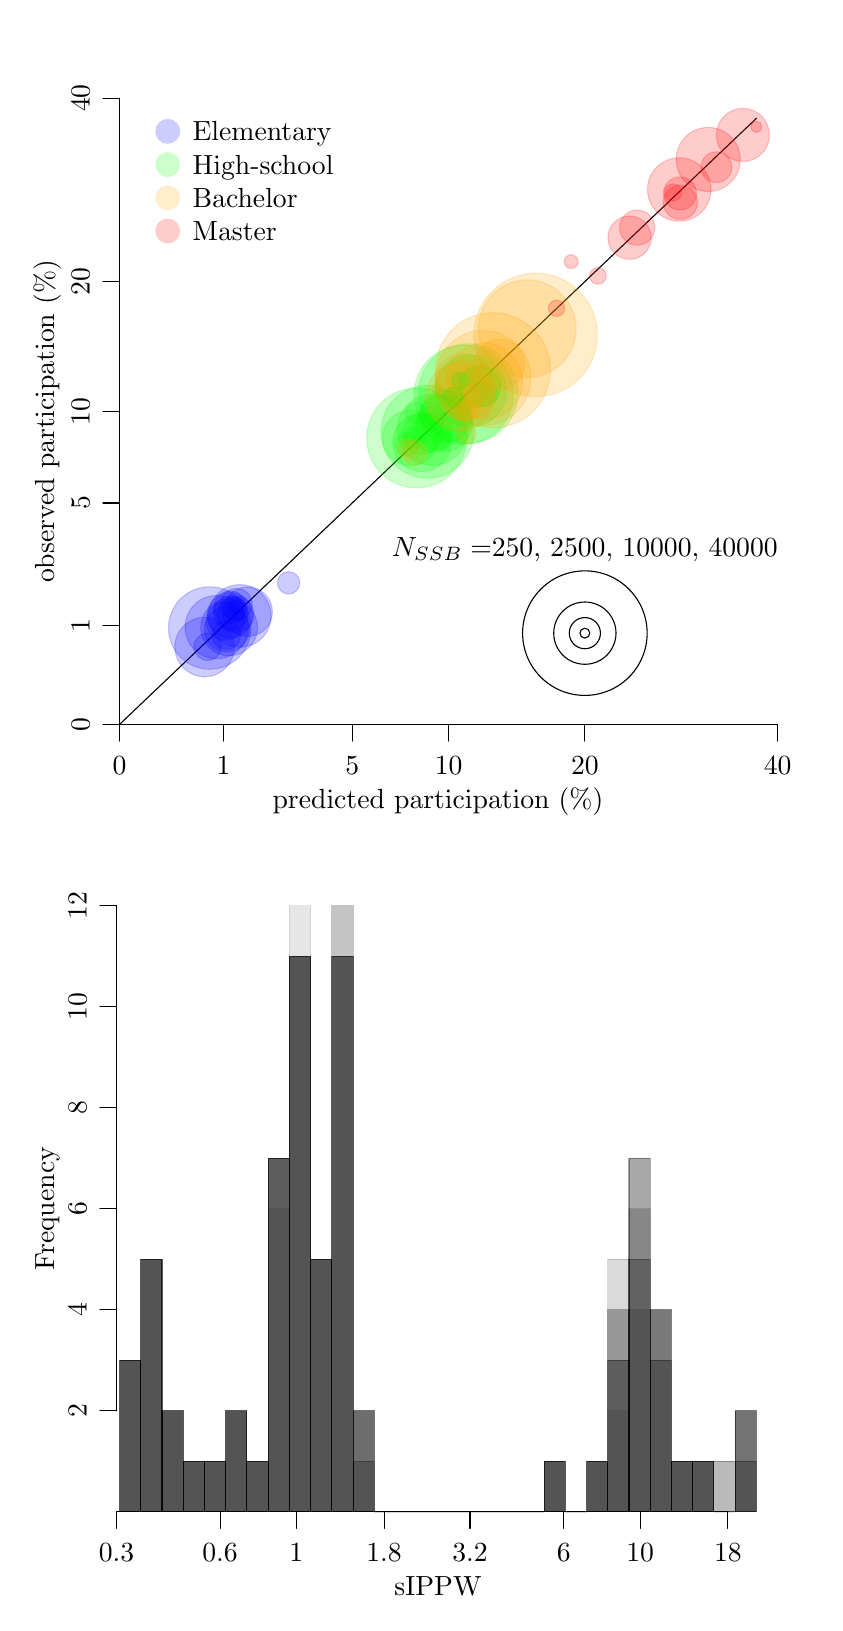
\begin{tikzpicture}[x=1pt,y=1pt]
\definecolor{fillColor}{RGB}{255,255,255}
\path[use as bounding box,fill=fillColor,fill opacity=0.00] (0,0) rectangle (284.53,569.06);
\begin{scope}
\path[clip] (  0.00,284.53) rectangle (284.53,569.06);
\definecolor{drawColor}{RGB}{0,0,0}

\node[text=drawColor,anchor=base,inner sep=0pt, outer sep=0pt, scale=  1.00] at (148.26,286.93) {predicted participation (\%)};

\node[text=drawColor,rotate= 90.00,anchor=base,inner sep=0pt, outer sep=0pt, scale=  1.00] at (  9.60,426.79) {observed participation (\%)};
\end{scope}
\begin{scope}
\path[clip] ( 24.00,308.53) rectangle (272.53,545.06);
\definecolor{drawColor}{RGB}{0,0,0}

\path[draw=drawColor,line width= 0.4pt,line join=round,line cap=round] ( 33.20,317.29) --
	(263.32,536.29);
\definecolor{drawColor}{RGB}{0,0,255}
\definecolor{fillColor}{RGB}{0,0,255}

\path[draw=drawColor,draw opacity=0.20,line width= 0.4pt,line join=round,line cap=round,fill=fillColor,fill opacity=0.20] ( 76.64,356.48) circle ( 11.31);
\definecolor{drawColor}{RGB}{0,255,0}
\definecolor{fillColor}{RGB}{0,255,0}

\path[draw=drawColor,draw opacity=0.20,line width= 0.4pt,line join=round,line cap=round,fill=fillColor,fill opacity=0.20] (165.46,436.52) circle (  4.49);
\definecolor{drawColor}{RGB}{0,0,255}
\definecolor{fillColor}{RGB}{0,0,255}

\path[draw=drawColor,draw opacity=0.20,line width= 0.4pt,line join=round,line cap=round,fill=fillColor,fill opacity=0.20] ( 65.79,352.12) circle ( 14.91);

\path[draw=drawColor,draw opacity=0.20,line width= 0.4pt,line join=round,line cap=round,fill=fillColor,fill opacity=0.20] ( 63.93,345.25) circle ( 10.75);

\path[draw=drawColor,draw opacity=0.20,line width= 0.4pt,line join=round,line cap=round,fill=fillColor,fill opacity=0.20] ( 65.06,345.35) circle (  4.97);
\definecolor{drawColor}{RGB}{0,255,0}
\definecolor{fillColor}{RGB}{0,255,0}

\path[draw=drawColor,draw opacity=0.20,line width= 0.4pt,line join=round,line cap=round,fill=fillColor,fill opacity=0.20] (157.54,436.40) circle ( 17.91);

\path[draw=drawColor,draw opacity=0.20,line width= 0.4pt,line join=round,line cap=round,fill=fillColor,fill opacity=0.20] (142.51,419.20) circle ( 10.54);

\path[draw=drawColor,draw opacity=0.20,line width= 0.4pt,line join=round,line cap=round,fill=fillColor,fill opacity=0.20] (149.54,419.78) circle (  3.27);
\definecolor{drawColor}{RGB}{255,165,0}
\definecolor{fillColor}{RGB}{255,165,0}

\path[draw=drawColor,draw opacity=0.20,line width= 0.4pt,line join=round,line cap=round,fill=fillColor,fill opacity=0.20] (157.37,441.02) circle ( 10.29);

\path[draw=drawColor,draw opacity=0.20,line width= 0.4pt,line join=round,line cap=round,fill=fillColor,fill opacity=0.20] (146.02,427.83) circle (  4.47);
\definecolor{drawColor}{RGB}{0,0,255}
\definecolor{fillColor}{RGB}{0,0,255}

\path[draw=drawColor,draw opacity=0.20,line width= 0.4pt,line join=round,line cap=round,fill=fillColor,fill opacity=0.20] ( 72.79,352.34) circle ( 10.25);

\path[draw=drawColor,draw opacity=0.20,line width= 0.4pt,line join=round,line cap=round,fill=fillColor,fill opacity=0.20] ( 68.30,352.45) circle ( 11.43);

\path[draw=drawColor,draw opacity=0.20,line width= 0.4pt,line join=round,line cap=round,fill=fillColor,fill opacity=0.20] ( 72.00,351.64) circle (  8.16);

\path[draw=drawColor,draw opacity=0.20,line width= 0.4pt,line join=round,line cap=round,fill=fillColor,fill opacity=0.20] ( 71.81,349.49) circle (  5.14);
\definecolor{drawColor}{RGB}{0,255,0}
\definecolor{fillColor}{RGB}{0,255,0}

\path[draw=drawColor,draw opacity=0.20,line width= 0.4pt,line join=round,line cap=round,fill=fillColor,fill opacity=0.20] (159.14,436.87) circle ( 17.97);

\path[draw=drawColor,draw opacity=0.20,line width= 0.4pt,line join=round,line cap=round,fill=fillColor,fill opacity=0.20] (140.55,420.78) circle ( 18.04);

\path[draw=drawColor,draw opacity=0.20,line width= 0.4pt,line join=round,line cap=round,fill=fillColor,fill opacity=0.20] (138.29,420.79) circle ( 10.05);

\path[draw=drawColor,draw opacity=0.20,line width= 0.4pt,line join=round,line cap=round,fill=fillColor,fill opacity=0.20] (137.01,418.51) circle (  4.25);
\definecolor{drawColor}{RGB}{255,165,0}
\definecolor{fillColor}{RGB}{255,165,0}

\path[draw=drawColor,draw opacity=0.20,line width= 0.4pt,line join=round,line cap=round,fill=fillColor,fill opacity=0.20] (183.54,458.02) circle ( 22.31);

\path[draw=drawColor,draw opacity=0.20,line width= 0.4pt,line join=round,line cap=round,fill=fillColor,fill opacity=0.20] (164.63,442.49) circle ( 17.18);

\path[draw=drawColor,draw opacity=0.20,line width= 0.4pt,line join=round,line cap=round,fill=fillColor,fill opacity=0.20] (158.76,439.09) circle (  7.16);

\path[draw=drawColor,draw opacity=0.20,line width= 0.4pt,line join=round,line cap=round,fill=fillColor,fill opacity=0.20] (148.11,438.47) circle (  2.15);
\definecolor{drawColor}{RGB}{255,0,0}
\definecolor{fillColor}{RGB}{255,0,0}

\path[draw=drawColor,draw opacity=0.20,line width= 0.4pt,line join=round,line cap=round,fill=fillColor,fill opacity=0.20] (258.44,530.29) circle (  9.60);

\path[draw=drawColor,draw opacity=0.20,line width= 0.4pt,line join=round,line cap=round,fill=fillColor,fill opacity=0.20] (248.89,518.64) circle (  5.57);
\definecolor{drawColor}{RGB}{0,0,255}
\definecolor{fillColor}{RGB}{0,0,255}

\path[draw=drawColor,draw opacity=0.20,line width= 0.4pt,line join=round,line cap=round,fill=fillColor,fill opacity=0.20] ( 75.15,357.12) circle (  6.61);

\path[draw=drawColor,draw opacity=0.20,line width= 0.4pt,line join=round,line cap=round,fill=fillColor,fill opacity=0.20] ( 79.48,358.01) circle (  8.95);

\path[draw=drawColor,draw opacity=0.20,line width= 0.4pt,line join=round,line cap=round,fill=fillColor,fill opacity=0.20] ( 73.08,356.72) circle (  8.22);

\path[draw=drawColor,draw opacity=0.20,line width= 0.4pt,line join=round,line cap=round,fill=fillColor,fill opacity=0.20] ( 71.38,354.64) circle (  6.92);
\definecolor{drawColor}{RGB}{0,255,0}
\definecolor{fillColor}{RGB}{0,255,0}

\path[draw=drawColor,draw opacity=0.20,line width= 0.4pt,line join=round,line cap=round,fill=fillColor,fill opacity=0.20] (160.11,437.86) circle ( 12.98);

\path[draw=drawColor,draw opacity=0.20,line width= 0.4pt,line join=round,line cap=round,fill=fillColor,fill opacity=0.20] (144.43,423.04) circle ( 16.77);

\path[draw=drawColor,draw opacity=0.20,line width= 0.4pt,line join=round,line cap=round,fill=fillColor,fill opacity=0.20] (146.32,423.69) circle ( 12.77);

\path[draw=drawColor,draw opacity=0.20,line width= 0.4pt,line join=round,line cap=round,fill=fillColor,fill opacity=0.20] (142.51,422.16) circle (  7.29);
\definecolor{drawColor}{RGB}{255,165,0}
\definecolor{fillColor}{RGB}{255,165,0}

\path[draw=drawColor,draw opacity=0.20,line width= 0.4pt,line join=round,line cap=round,fill=fillColor,fill opacity=0.20] (180.52,460.28) circle ( 17.65);

\path[draw=drawColor,draw opacity=0.20,line width= 0.4pt,line join=round,line cap=round,fill=fillColor,fill opacity=0.20] (168.11,445.27) circle ( 20.81);

\path[draw=drawColor,draw opacity=0.20,line width= 0.4pt,line join=round,line cap=round,fill=fillColor,fill opacity=0.20] (165.01,441.22) circle ( 13.85);

\path[draw=drawColor,draw opacity=0.20,line width= 0.4pt,line join=round,line cap=round,fill=fillColor,fill opacity=0.20] (165.39,441.63) circle (  5.75);
\definecolor{drawColor}{RGB}{255,0,0}
\definecolor{fillColor}{RGB}{255,0,0}

\path[draw=drawColor,draw opacity=0.20,line width= 0.4pt,line join=round,line cap=round,fill=fillColor,fill opacity=0.20] (245.92,521.43) circle ( 11.58);

\path[draw=drawColor,draw opacity=0.20,line width= 0.4pt,line join=round,line cap=round,fill=fillColor,fill opacity=0.20] (235.45,510.59) circle ( 11.47);

\path[draw=drawColor,draw opacity=0.20,line width= 0.4pt,line join=round,line cap=round,fill=fillColor,fill opacity=0.20] (235.71,509.15) circle (  5.98);

\path[draw=drawColor,draw opacity=0.20,line width= 0.4pt,line join=round,line cap=round,fill=fillColor,fill opacity=0.20] (263.32,533.20) circle (  2.05);
\definecolor{drawColor}{RGB}{0,0,255}
\definecolor{fillColor}{RGB}{0,0,255}

\path[draw=drawColor,draw opacity=0.20,line width= 0.4pt,line join=round,line cap=round,fill=fillColor,fill opacity=0.20] ( 94.29,368.45) circle (  4.04);

\path[draw=drawColor,draw opacity=0.20,line width= 0.4pt,line join=round,line cap=round,fill=fillColor,fill opacity=0.20] ( 75.38,360.68) circle (  5.76);

\path[draw=drawColor,draw opacity=0.20,line width= 0.4pt,line join=round,line cap=round,fill=fillColor,fill opacity=0.20] ( 73.17,359.61) circle (  5.89);

\path[draw=drawColor,draw opacity=0.20,line width= 0.4pt,line join=round,line cap=round,fill=fillColor,fill opacity=0.20] ( 73.37,357.58) circle (  6.23);
\definecolor{drawColor}{RGB}{0,255,0}
\definecolor{fillColor}{RGB}{0,255,0}

\path[draw=drawColor,draw opacity=0.20,line width= 0.4pt,line join=round,line cap=round,fill=fillColor,fill opacity=0.20] (163.36,439.42) circle (  7.49);

\path[draw=drawColor,draw opacity=0.20,line width= 0.4pt,line join=round,line cap=round,fill=fillColor,fill opacity=0.20] (150.46,426.03) circle ( 10.18);

\path[draw=drawColor,draw opacity=0.20,line width= 0.4pt,line join=round,line cap=round,fill=fillColor,fill opacity=0.20] (151.04,428.52) circle (  9.37);

\path[draw=drawColor,draw opacity=0.20,line width= 0.4pt,line join=round,line cap=round,fill=fillColor,fill opacity=0.20] (146.05,422.94) circle (  7.08);
\definecolor{drawColor}{RGB}{255,165,0}
\definecolor{fillColor}{RGB}{255,165,0}

\path[draw=drawColor,draw opacity=0.20,line width= 0.4pt,line join=round,line cap=round,fill=fillColor,fill opacity=0.20] (170.47,447.33) circle (  9.22);

\path[draw=drawColor,draw opacity=0.20,line width= 0.4pt,line join=round,line cap=round,fill=fillColor,fill opacity=0.20] (156.10,435.50) circle ( 12.29);

\path[draw=drawColor,draw opacity=0.20,line width= 0.4pt,line join=round,line cap=round,fill=fillColor,fill opacity=0.20] (158.29,438.18) circle ( 10.90);

\path[draw=drawColor,draw opacity=0.20,line width= 0.4pt,line join=round,line cap=round,fill=fillColor,fill opacity=0.20] (157.17,433.86) circle (  6.63);
\definecolor{drawColor}{RGB}{255,0,0}
\definecolor{fillColor}{RGB}{255,0,0}

\path[draw=drawColor,draw opacity=0.20,line width= 0.4pt,line join=round,line cap=round,fill=fillColor,fill opacity=0.20] (235.84,505.97) circle (  6.20);

\path[draw=drawColor,draw opacity=0.20,line width= 0.4pt,line join=round,line cap=round,fill=fillColor,fill opacity=0.20] (217.51,493.17) circle (  7.84);

\path[draw=drawColor,draw opacity=0.20,line width= 0.4pt,line join=round,line cap=round,fill=fillColor,fill opacity=0.20] (220.25,496.79) circle (  6.37);

\path[draw=drawColor,draw opacity=0.20,line width= 0.4pt,line join=round,line cap=round,fill=fillColor,fill opacity=0.20] (233.23,509.52) circle (  3.08);
\definecolor{drawColor}{RGB}{0,0,255}
\definecolor{fillColor}{RGB}{0,0,255}

\path[draw=drawColor,draw opacity=0.20,line width= 0.4pt,line join=round,line cap=round,fill=fillColor,fill opacity=0.20] ( 74.92,360.26) circle (  3.04);

\path[draw=drawColor,draw opacity=0.20,line width= 0.4pt,line join=round,line cap=round,fill=fillColor,fill opacity=0.20] ( 75.74,360.28) circle (  2.63);

\path[draw=drawColor,draw opacity=0.20,line width= 0.4pt,line join=round,line cap=round,fill=fillColor,fill opacity=0.20] ( 74.98,358.18) circle (  3.65);
\definecolor{drawColor}{RGB}{0,255,0}
\definecolor{fillColor}{RGB}{0,255,0}

\path[draw=drawColor,draw opacity=0.20,line width= 0.4pt,line join=round,line cap=round,fill=fillColor,fill opacity=0.20] (156.18,441.58) circle (  2.92);

\path[draw=drawColor,draw opacity=0.20,line width= 0.4pt,line join=round,line cap=round,fill=fillColor,fill opacity=0.20] (140.26,429.84) circle (  3.75);

\path[draw=drawColor,draw opacity=0.20,line width= 0.4pt,line join=round,line cap=round,fill=fillColor,fill opacity=0.20] (153.87,435.57) circle (  3.56);

\path[draw=drawColor,draw opacity=0.20,line width= 0.4pt,line join=round,line cap=round,fill=fillColor,fill opacity=0.20] (139.84,420.99) circle (  3.72);
\definecolor{drawColor}{RGB}{255,165,0}
\definecolor{fillColor}{RGB}{255,165,0}

\path[draw=drawColor,draw opacity=0.20,line width= 0.4pt,line join=round,line cap=round,fill=fillColor,fill opacity=0.20] (158.59,422.23) circle (  3.59);

\path[draw=drawColor,draw opacity=0.20,line width= 0.4pt,line join=round,line cap=round,fill=fillColor,fill opacity=0.20] (139.85,415.47) circle (  4.45);

\path[draw=drawColor,draw opacity=0.20,line width= 0.4pt,line join=round,line cap=round,fill=fillColor,fill opacity=0.20] (158.08,430.36) circle (  3.99);

\path[draw=drawColor,draw opacity=0.20,line width= 0.4pt,line join=round,line cap=round,fill=fillColor,fill opacity=0.20] (137.28,416.89) circle (  3.63);
\definecolor{drawColor}{RGB}{255,0,0}
\definecolor{fillColor}{RGB}{255,0,0}

\path[draw=drawColor,draw opacity=0.20,line width= 0.4pt,line join=round,line cap=round,fill=fillColor,fill opacity=0.20] (196.38,484.52) circle (  2.51);

\path[draw=drawColor,draw opacity=0.20,line width= 0.4pt,line join=round,line cap=round,fill=fillColor,fill opacity=0.20] (191.11,467.64) circle (  2.95);

\path[draw=drawColor,draw opacity=0.20,line width= 0.4pt,line join=round,line cap=round,fill=fillColor,fill opacity=0.20] (206.04,479.39) circle (  3.03);
\end{scope}
\begin{scope}
\path[clip] (  0.00,  0.00) rectangle (284.53,569.06);
\definecolor{drawColor}{RGB}{0,0,0}

\path[draw=drawColor,line width= 0.4pt,line join=round,line cap=round] ( 33.20,317.29) -- (270.99,317.29);

\path[draw=drawColor,line width= 0.4pt,line join=round,line cap=round] ( 33.20,317.29) -- ( 33.20,311.29);

\path[draw=drawColor,line width= 0.4pt,line join=round,line cap=round] ( 70.80,317.29) -- ( 70.80,311.29);

\path[draw=drawColor,line width= 0.4pt,line join=round,line cap=round] (117.27,317.29) -- (117.27,311.29);

\path[draw=drawColor,line width= 0.4pt,line join=round,line cap=round] (152.10,317.29) -- (152.10,311.29);

\path[draw=drawColor,line width= 0.4pt,line join=round,line cap=round] (201.34,317.29) -- (201.34,311.29);

\path[draw=drawColor,line width= 0.4pt,line join=round,line cap=round] (270.99,317.29) -- (270.99,311.29);

\node[text=drawColor,anchor=base,inner sep=0pt, outer sep=0pt, scale=  1.00] at ( 33.20,299.29) {0};

\node[text=drawColor,anchor=base,inner sep=0pt, outer sep=0pt, scale=  1.00] at ( 70.80,299.29) {1};

\node[text=drawColor,anchor=base,inner sep=0pt, outer sep=0pt, scale=  1.00] at (117.27,299.29) {5};

\node[text=drawColor,anchor=base,inner sep=0pt, outer sep=0pt, scale=  1.00] at (152.10,299.29) {10};

\node[text=drawColor,anchor=base,inner sep=0pt, outer sep=0pt, scale=  1.00] at (201.34,299.29) {20};

\node[text=drawColor,anchor=base,inner sep=0pt, outer sep=0pt, scale=  1.00] at (270.99,299.29) {40};

\path[draw=drawColor,line width= 0.4pt,line join=round,line cap=round] ( 33.20,317.29) -- ( 33.20,543.59);

\path[draw=drawColor,line width= 0.4pt,line join=round,line cap=round] ( 33.20,317.29) -- ( 27.20,317.29);

\path[draw=drawColor,line width= 0.4pt,line join=round,line cap=round] ( 33.20,353.07) -- ( 27.20,353.07);

\path[draw=drawColor,line width= 0.4pt,line join=round,line cap=round] ( 33.20,397.30) -- ( 27.20,397.30);

\path[draw=drawColor,line width= 0.4pt,line join=round,line cap=round] ( 33.20,430.44) -- ( 27.20,430.44);

\path[draw=drawColor,line width= 0.4pt,line join=round,line cap=round] ( 33.20,477.31) -- ( 27.20,477.31);

\path[draw=drawColor,line width= 0.4pt,line join=round,line cap=round] ( 33.20,543.59) -- ( 27.20,543.59);

\node[text=drawColor,rotate= 90.00,anchor=base,inner sep=0pt, outer sep=0pt, scale=  1.00] at ( 22.40,317.29) {0};

\node[text=drawColor,rotate= 90.00,anchor=base,inner sep=0pt, outer sep=0pt, scale=  1.00] at ( 22.40,353.07) {1};

\node[text=drawColor,rotate= 90.00,anchor=base,inner sep=0pt, outer sep=0pt, scale=  1.00] at ( 22.40,397.30) {5};

\node[text=drawColor,rotate= 90.00,anchor=base,inner sep=0pt, outer sep=0pt, scale=  1.00] at ( 22.40,430.44) {10};

\node[text=drawColor,rotate= 90.00,anchor=base,inner sep=0pt, outer sep=0pt, scale=  1.00] at ( 22.40,477.31) {20};

\node[text=drawColor,rotate= 90.00,anchor=base,inner sep=0pt, outer sep=0pt, scale=  1.00] at ( 22.40,543.59) {40};
\end{scope}
\begin{scope}
\path[clip] ( 24.00,308.53) rectangle (272.53,545.06);
\definecolor{drawColor}{RGB}{0,0,0}

\path[draw=drawColor,line width= 0.4pt,line join=round,line cap=round] (201.34,350.27) circle (  1.78);

\path[draw=drawColor,line width= 0.4pt,line join=round,line cap=round] (201.34,350.27) circle (  5.63);

\path[draw=drawColor,line width= 0.4pt,line join=round,line cap=round] (201.34,350.27) circle ( 11.25);

\path[draw=drawColor,line width= 0.4pt,line join=round,line cap=round] (201.34,350.27) circle ( 22.50);

\node[text=drawColor,anchor=base,inner sep=0pt, outer sep=0pt, scale=  1.00] at (201.34,377.94) {$N_{SSB}=$250, 2500, 10000, 40000};
\definecolor{fillColor}{RGB}{0,0,255}

\path[fill=fillColor,fill opacity=0.20] ( 50.61,531.59) circle (  4.50);
\definecolor{fillColor}{RGB}{0,255,0}

\path[fill=fillColor,fill opacity=0.20] ( 50.61,519.59) circle (  4.50);
\definecolor{fillColor}{RGB}{255,165,0}

\path[fill=fillColor,fill opacity=0.20] ( 50.61,507.59) circle (  4.50);
\definecolor{fillColor}{RGB}{255,0,0}

\path[fill=fillColor,fill opacity=0.20] ( 50.61,495.59) circle (  4.50);

\node[text=drawColor,anchor=base west,inner sep=0pt, outer sep=0pt, scale=  1.00] at ( 59.61,528.15) {Elementary};

\node[text=drawColor,anchor=base west,inner sep=0pt, outer sep=0pt, scale=  1.00] at ( 59.61,516.15) {High-school};

\node[text=drawColor,anchor=base west,inner sep=0pt, outer sep=0pt, scale=  1.00] at ( 59.61,504.15) {Bachelor};

\node[text=drawColor,anchor=base west,inner sep=0pt, outer sep=0pt, scale=  1.00] at ( 59.61,492.15) {Master};
\end{scope}
\begin{scope}
\path[clip] (  0.00,  0.00) rectangle (284.53,284.53);
\definecolor{drawColor}{RGB}{0,0,0}

\node[text=drawColor,anchor=base,inner sep=0pt, outer sep=0pt, scale=  1.00] at (148.26,  2.40) {sIPPW};

\node[text=drawColor,rotate= 90.00,anchor=base,inner sep=0pt, outer sep=0pt, scale=  1.00] at (  9.60,142.26) {Frequency};
\end{scope}
\begin{scope}
\path[clip] ( 24.00, 24.00) rectangle (272.53,260.53);
\definecolor{drawColor}{RGB}{0,0,0}
\definecolor{fillColor}{RGB}{0,0,0}

\path[draw=drawColor,draw opacity=0.05,line width= 0.4pt,line join=round,line cap=round,fill=fillColor,fill opacity=0.10] ( 33.20, 32.76) rectangle ( 40.88, 87.51);

\path[draw=drawColor,draw opacity=0.05,line width= 0.4pt,line join=round,line cap=round,fill=fillColor,fill opacity=0.10] ( 40.88, 32.76) rectangle ( 48.55,124.01);

\path[draw=drawColor,draw opacity=0.05,line width= 0.4pt,line join=round,line cap=round,fill=fillColor,fill opacity=0.10] ( 48.55, 32.76) rectangle ( 56.22, 69.26);

\path[draw=drawColor,draw opacity=0.05,line width= 0.4pt,line join=round,line cap=round,fill=fillColor,fill opacity=0.10] ( 56.22, 32.76) rectangle ( 63.89, 51.01);

\path[draw=drawColor,draw opacity=0.05,line width= 0.4pt,line join=round,line cap=round,fill=fillColor,fill opacity=0.10] ( 63.89, 32.76) rectangle ( 71.56, 51.01);

\path[draw=drawColor,draw opacity=0.05,line width= 0.4pt,line join=round,line cap=round,fill=fillColor,fill opacity=0.10] ( 71.56, 32.76) rectangle ( 79.23, 69.26);

\path[draw=drawColor,draw opacity=0.05,line width= 0.4pt,line join=round,line cap=round,fill=fillColor,fill opacity=0.10] ( 79.23, 32.76) rectangle ( 86.90, 51.01);

\path[draw=drawColor,draw opacity=0.05,line width= 0.4pt,line join=round,line cap=round,fill=fillColor,fill opacity=0.10] ( 86.90, 32.76) rectangle ( 94.57,160.51);

\path[draw=drawColor,draw opacity=0.05,line width= 0.4pt,line join=round,line cap=round,fill=fillColor,fill opacity=0.10] ( 94.57, 32.76) rectangle (102.24,233.52);

\path[draw=drawColor,draw opacity=0.05,line width= 0.4pt,line join=round,line cap=round,fill=fillColor,fill opacity=0.10] (102.24, 32.76) rectangle (109.91,124.01);

\path[draw=drawColor,draw opacity=0.05,line width= 0.4pt,line join=round,line cap=round,fill=fillColor,fill opacity=0.10] (109.91, 32.76) rectangle (117.58,233.52);

\path[draw=drawColor,draw opacity=0.05,line width= 0.4pt,line join=round,line cap=round,fill=fillColor,fill opacity=0.10] (117.58, 32.76) rectangle (125.25, 69.26);

\path[draw=drawColor,draw opacity=0.05,line width= 0.4pt,line join=round,line cap=round,fill=fillColor,fill opacity=0.10] (125.25, 32.76) rectangle (132.92, 32.76);

\path[draw=drawColor,draw opacity=0.05,line width= 0.4pt,line join=round,line cap=round,fill=fillColor,fill opacity=0.10] (132.92, 32.76) rectangle (140.59, 32.76);

\path[draw=drawColor,draw opacity=0.05,line width= 0.4pt,line join=round,line cap=round,fill=fillColor,fill opacity=0.10] (140.59, 32.76) rectangle (148.26, 32.76);

\path[draw=drawColor,draw opacity=0.05,line width= 0.4pt,line join=round,line cap=round,fill=fillColor,fill opacity=0.10] (148.26, 32.76) rectangle (155.93, 32.76);

\path[draw=drawColor,draw opacity=0.05,line width= 0.4pt,line join=round,line cap=round,fill=fillColor,fill opacity=0.10] (155.93, 32.76) rectangle (163.60, 32.76);

\path[draw=drawColor,draw opacity=0.05,line width= 0.4pt,line join=round,line cap=round,fill=fillColor,fill opacity=0.10] (163.60, 32.76) rectangle (171.28, 32.76);

\path[draw=drawColor,draw opacity=0.05,line width= 0.4pt,line join=round,line cap=round,fill=fillColor,fill opacity=0.10] (171.28, 32.76) rectangle (178.95, 32.76);

\path[draw=drawColor,draw opacity=0.05,line width= 0.4pt,line join=round,line cap=round,fill=fillColor,fill opacity=0.10] (178.95, 32.76) rectangle (186.62, 32.76);

\path[draw=drawColor,draw opacity=0.05,line width= 0.4pt,line join=round,line cap=round,fill=fillColor,fill opacity=0.10] (186.62, 32.76) rectangle (194.29, 51.01);

\path[draw=drawColor,draw opacity=0.05,line width= 0.4pt,line join=round,line cap=round,fill=fillColor,fill opacity=0.10] (194.29, 32.76) rectangle (201.96, 32.76);

\path[draw=drawColor,draw opacity=0.05,line width= 0.4pt,line join=round,line cap=round,fill=fillColor,fill opacity=0.10] (201.96, 32.76) rectangle (209.63, 51.01);

\path[draw=drawColor,draw opacity=0.05,line width= 0.4pt,line join=round,line cap=round,fill=fillColor,fill opacity=0.10] (209.63, 32.76) rectangle (217.30, 87.51);

\path[draw=drawColor,draw opacity=0.05,line width= 0.4pt,line join=round,line cap=round,fill=fillColor,fill opacity=0.10] (217.30, 32.76) rectangle (224.97,142.26);

\path[draw=drawColor,draw opacity=0.05,line width= 0.4pt,line join=round,line cap=round,fill=fillColor,fill opacity=0.10] (224.97, 32.76) rectangle (232.64,105.76);

\path[draw=drawColor,draw opacity=0.05,line width= 0.4pt,line join=round,line cap=round,fill=fillColor,fill opacity=0.10] (232.64, 32.76) rectangle (240.31, 51.01);

\path[draw=drawColor,draw opacity=0.05,line width= 0.4pt,line join=round,line cap=round,fill=fillColor,fill opacity=0.10] (240.31, 32.76) rectangle (247.98, 51.01);

\path[draw=drawColor,draw opacity=0.05,line width= 0.4pt,line join=round,line cap=round,fill=fillColor,fill opacity=0.10] (247.98, 32.76) rectangle (255.65, 32.76);

\path[draw=drawColor,draw opacity=0.05,line width= 0.4pt,line join=round,line cap=round,fill=fillColor,fill opacity=0.10] (255.65, 32.76) rectangle (263.32, 69.26);
\definecolor{fillColor}{RGB}{0,0,0}

\path[draw=drawColor,draw opacity=0.05,line width= 0.4pt,line join=round,line cap=round,fill=fillColor,fill opacity=0.05] ( 33.20, 32.76) rectangle ( 40.88, 87.51);

\path[draw=drawColor,draw opacity=0.05,line width= 0.4pt,line join=round,line cap=round,fill=fillColor,fill opacity=0.05] ( 40.88, 32.76) rectangle ( 48.55,124.01);

\path[draw=drawColor,draw opacity=0.05,line width= 0.4pt,line join=round,line cap=round,fill=fillColor,fill opacity=0.05] ( 48.55, 32.76) rectangle ( 56.22, 69.26);

\path[draw=drawColor,draw opacity=0.05,line width= 0.4pt,line join=round,line cap=round,fill=fillColor,fill opacity=0.05] ( 56.22, 32.76) rectangle ( 63.89, 51.01);

\path[draw=drawColor,draw opacity=0.05,line width= 0.4pt,line join=round,line cap=round,fill=fillColor,fill opacity=0.05] ( 63.89, 32.76) rectangle ( 71.56, 51.01);

\path[draw=drawColor,draw opacity=0.05,line width= 0.4pt,line join=round,line cap=round,fill=fillColor,fill opacity=0.05] ( 71.56, 32.76) rectangle ( 79.23, 69.26);

\path[draw=drawColor,draw opacity=0.05,line width= 0.4pt,line join=round,line cap=round,fill=fillColor,fill opacity=0.05] ( 79.23, 32.76) rectangle ( 86.90, 51.01);

\path[draw=drawColor,draw opacity=0.05,line width= 0.4pt,line join=round,line cap=round,fill=fillColor,fill opacity=0.05] ( 86.90, 32.76) rectangle ( 94.57,160.51);

\path[draw=drawColor,draw opacity=0.05,line width= 0.4pt,line join=round,line cap=round,fill=fillColor,fill opacity=0.05] ( 94.57, 32.76) rectangle (102.24,233.52);

\path[draw=drawColor,draw opacity=0.05,line width= 0.4pt,line join=round,line cap=round,fill=fillColor,fill opacity=0.05] (102.24, 32.76) rectangle (109.91,124.01);

\path[draw=drawColor,draw opacity=0.05,line width= 0.4pt,line join=round,line cap=round,fill=fillColor,fill opacity=0.05] (109.91, 32.76) rectangle (117.58,251.77);

\path[draw=drawColor,draw opacity=0.05,line width= 0.4pt,line join=round,line cap=round,fill=fillColor,fill opacity=0.05] (117.58, 32.76) rectangle (125.25, 51.01);

\path[draw=drawColor,draw opacity=0.05,line width= 0.4pt,line join=round,line cap=round,fill=fillColor,fill opacity=0.05] (125.25, 32.76) rectangle (132.92, 32.76);

\path[draw=drawColor,draw opacity=0.05,line width= 0.4pt,line join=round,line cap=round,fill=fillColor,fill opacity=0.05] (132.92, 32.76) rectangle (140.59, 32.76);

\path[draw=drawColor,draw opacity=0.05,line width= 0.4pt,line join=round,line cap=round,fill=fillColor,fill opacity=0.05] (140.59, 32.76) rectangle (148.26, 32.76);

\path[draw=drawColor,draw opacity=0.05,line width= 0.4pt,line join=round,line cap=round,fill=fillColor,fill opacity=0.05] (148.26, 32.76) rectangle (155.93, 32.76);

\path[draw=drawColor,draw opacity=0.05,line width= 0.4pt,line join=round,line cap=round,fill=fillColor,fill opacity=0.05] (155.93, 32.76) rectangle (163.60, 32.76);

\path[draw=drawColor,draw opacity=0.05,line width= 0.4pt,line join=round,line cap=round,fill=fillColor,fill opacity=0.05] (163.60, 32.76) rectangle (171.28, 32.76);

\path[draw=drawColor,draw opacity=0.05,line width= 0.4pt,line join=round,line cap=round,fill=fillColor,fill opacity=0.05] (171.28, 32.76) rectangle (178.95, 32.76);

\path[draw=drawColor,draw opacity=0.05,line width= 0.4pt,line join=round,line cap=round,fill=fillColor,fill opacity=0.05] (178.95, 32.76) rectangle (186.62, 32.76);

\path[draw=drawColor,draw opacity=0.05,line width= 0.4pt,line join=round,line cap=round,fill=fillColor,fill opacity=0.05] (186.62, 32.76) rectangle (194.29, 51.01);

\path[draw=drawColor,draw opacity=0.05,line width= 0.4pt,line join=round,line cap=round,fill=fillColor,fill opacity=0.05] (194.29, 32.76) rectangle (201.96, 32.76);

\path[draw=drawColor,draw opacity=0.05,line width= 0.4pt,line join=round,line cap=round,fill=fillColor,fill opacity=0.05] (201.96, 32.76) rectangle (209.63, 51.01);

\path[draw=drawColor,draw opacity=0.05,line width= 0.4pt,line join=round,line cap=round,fill=fillColor,fill opacity=0.05] (209.63, 32.76) rectangle (217.30, 87.51);

\path[draw=drawColor,draw opacity=0.05,line width= 0.4pt,line join=round,line cap=round,fill=fillColor,fill opacity=0.05] (217.30, 32.76) rectangle (224.97,160.51);

\path[draw=drawColor,draw opacity=0.05,line width= 0.4pt,line join=round,line cap=round,fill=fillColor,fill opacity=0.05] (224.97, 32.76) rectangle (232.64, 87.51);

\path[draw=drawColor,draw opacity=0.05,line width= 0.4pt,line join=round,line cap=round,fill=fillColor,fill opacity=0.05] (232.64, 32.76) rectangle (240.31, 51.01);

\path[draw=drawColor,draw opacity=0.05,line width= 0.4pt,line join=round,line cap=round,fill=fillColor,fill opacity=0.05] (240.31, 32.76) rectangle (247.98, 51.01);

\path[draw=drawColor,draw opacity=0.05,line width= 0.4pt,line join=round,line cap=round,fill=fillColor,fill opacity=0.05] (247.98, 32.76) rectangle (255.65, 32.76);

\path[draw=drawColor,draw opacity=0.05,line width= 0.4pt,line join=round,line cap=round,fill=fillColor,fill opacity=0.05] (255.65, 32.76) rectangle (263.32, 69.26);

\path[draw=drawColor,draw opacity=0.05,line width= 0.4pt,line join=round,line cap=round,fill=fillColor,fill opacity=0.05] ( 33.20, 32.76) rectangle ( 40.88, 87.51);

\path[draw=drawColor,draw opacity=0.05,line width= 0.4pt,line join=round,line cap=round,fill=fillColor,fill opacity=0.05] ( 40.88, 32.76) rectangle ( 48.55,124.01);

\path[draw=drawColor,draw opacity=0.05,line width= 0.4pt,line join=round,line cap=round,fill=fillColor,fill opacity=0.05] ( 48.55, 32.76) rectangle ( 56.22, 69.26);

\path[draw=drawColor,draw opacity=0.05,line width= 0.4pt,line join=round,line cap=round,fill=fillColor,fill opacity=0.05] ( 56.22, 32.76) rectangle ( 63.89, 51.01);

\path[draw=drawColor,draw opacity=0.05,line width= 0.4pt,line join=round,line cap=round,fill=fillColor,fill opacity=0.05] ( 63.89, 32.76) rectangle ( 71.56, 51.01);

\path[draw=drawColor,draw opacity=0.05,line width= 0.4pt,line join=round,line cap=round,fill=fillColor,fill opacity=0.05] ( 71.56, 32.76) rectangle ( 79.23, 69.26);

\path[draw=drawColor,draw opacity=0.05,line width= 0.4pt,line join=round,line cap=round,fill=fillColor,fill opacity=0.05] ( 79.23, 32.76) rectangle ( 86.90, 51.01);

\path[draw=drawColor,draw opacity=0.05,line width= 0.4pt,line join=round,line cap=round,fill=fillColor,fill opacity=0.05] ( 86.90, 32.76) rectangle ( 94.57,142.26);

\path[draw=drawColor,draw opacity=0.05,line width= 0.4pt,line join=round,line cap=round,fill=fillColor,fill opacity=0.05] ( 94.57, 32.76) rectangle (102.24,251.77);

\path[draw=drawColor,draw opacity=0.05,line width= 0.4pt,line join=round,line cap=round,fill=fillColor,fill opacity=0.05] (102.24, 32.76) rectangle (109.91,124.01);

\path[draw=drawColor,draw opacity=0.05,line width= 0.4pt,line join=round,line cap=round,fill=fillColor,fill opacity=0.05] (109.91, 32.76) rectangle (117.58,233.52);

\path[draw=drawColor,draw opacity=0.05,line width= 0.4pt,line join=round,line cap=round,fill=fillColor,fill opacity=0.05] (117.58, 32.76) rectangle (125.25, 69.26);

\path[draw=drawColor,draw opacity=0.05,line width= 0.4pt,line join=round,line cap=round,fill=fillColor,fill opacity=0.05] (125.25, 32.76) rectangle (132.92, 32.76);

\path[draw=drawColor,draw opacity=0.05,line width= 0.4pt,line join=round,line cap=round,fill=fillColor,fill opacity=0.05] (132.92, 32.76) rectangle (140.59, 32.76);

\path[draw=drawColor,draw opacity=0.05,line width= 0.4pt,line join=round,line cap=round,fill=fillColor,fill opacity=0.05] (140.59, 32.76) rectangle (148.26, 32.76);

\path[draw=drawColor,draw opacity=0.05,line width= 0.4pt,line join=round,line cap=round,fill=fillColor,fill opacity=0.05] (148.26, 32.76) rectangle (155.93, 32.76);

\path[draw=drawColor,draw opacity=0.05,line width= 0.4pt,line join=round,line cap=round,fill=fillColor,fill opacity=0.05] (155.93, 32.76) rectangle (163.60, 32.76);

\path[draw=drawColor,draw opacity=0.05,line width= 0.4pt,line join=round,line cap=round,fill=fillColor,fill opacity=0.05] (163.60, 32.76) rectangle (171.28, 32.76);

\path[draw=drawColor,draw opacity=0.05,line width= 0.4pt,line join=round,line cap=round,fill=fillColor,fill opacity=0.05] (171.28, 32.76) rectangle (178.95, 32.76);

\path[draw=drawColor,draw opacity=0.05,line width= 0.4pt,line join=round,line cap=round,fill=fillColor,fill opacity=0.05] (178.95, 32.76) rectangle (186.62, 32.76);

\path[draw=drawColor,draw opacity=0.05,line width= 0.4pt,line join=round,line cap=round,fill=fillColor,fill opacity=0.05] (186.62, 32.76) rectangle (194.29, 51.01);

\path[draw=drawColor,draw opacity=0.05,line width= 0.4pt,line join=round,line cap=round,fill=fillColor,fill opacity=0.05] (194.29, 32.76) rectangle (201.96, 32.76);

\path[draw=drawColor,draw opacity=0.05,line width= 0.4pt,line join=round,line cap=round,fill=fillColor,fill opacity=0.05] (201.96, 32.76) rectangle (209.63, 51.01);

\path[draw=drawColor,draw opacity=0.05,line width= 0.4pt,line join=round,line cap=round,fill=fillColor,fill opacity=0.05] (209.63, 32.76) rectangle (217.30,105.76);

\path[draw=drawColor,draw opacity=0.05,line width= 0.4pt,line join=round,line cap=round,fill=fillColor,fill opacity=0.05] (217.30, 32.76) rectangle (224.97,124.01);

\path[draw=drawColor,draw opacity=0.05,line width= 0.4pt,line join=round,line cap=round,fill=fillColor,fill opacity=0.05] (224.97, 32.76) rectangle (232.64,105.76);

\path[draw=drawColor,draw opacity=0.05,line width= 0.4pt,line join=round,line cap=round,fill=fillColor,fill opacity=0.05] (232.64, 32.76) rectangle (240.31, 51.01);

\path[draw=drawColor,draw opacity=0.05,line width= 0.4pt,line join=round,line cap=round,fill=fillColor,fill opacity=0.05] (240.31, 32.76) rectangle (247.98, 51.01);

\path[draw=drawColor,draw opacity=0.05,line width= 0.4pt,line join=round,line cap=round,fill=fillColor,fill opacity=0.05] (247.98, 32.76) rectangle (255.65, 51.01);

\path[draw=drawColor,draw opacity=0.05,line width= 0.4pt,line join=round,line cap=round,fill=fillColor,fill opacity=0.05] (255.65, 32.76) rectangle (263.32, 51.01);

\path[draw=drawColor,draw opacity=0.05,line width= 0.4pt,line join=round,line cap=round,fill=fillColor,fill opacity=0.05] ( 33.20, 32.76) rectangle ( 40.88, 87.51);

\path[draw=drawColor,draw opacity=0.05,line width= 0.4pt,line join=round,line cap=round,fill=fillColor,fill opacity=0.05] ( 40.88, 32.76) rectangle ( 48.55,124.01);

\path[draw=drawColor,draw opacity=0.05,line width= 0.4pt,line join=round,line cap=round,fill=fillColor,fill opacity=0.05] ( 48.55, 32.76) rectangle ( 56.22, 69.26);

\path[draw=drawColor,draw opacity=0.05,line width= 0.4pt,line join=round,line cap=round,fill=fillColor,fill opacity=0.05] ( 56.22, 32.76) rectangle ( 63.89, 51.01);

\path[draw=drawColor,draw opacity=0.05,line width= 0.4pt,line join=round,line cap=round,fill=fillColor,fill opacity=0.05] ( 63.89, 32.76) rectangle ( 71.56, 51.01);

\path[draw=drawColor,draw opacity=0.05,line width= 0.4pt,line join=round,line cap=round,fill=fillColor,fill opacity=0.05] ( 71.56, 32.76) rectangle ( 79.23, 69.26);

\path[draw=drawColor,draw opacity=0.05,line width= 0.4pt,line join=round,line cap=round,fill=fillColor,fill opacity=0.05] ( 79.23, 32.76) rectangle ( 86.90, 51.01);

\path[draw=drawColor,draw opacity=0.05,line width= 0.4pt,line join=round,line cap=round,fill=fillColor,fill opacity=0.05] ( 86.90, 32.76) rectangle ( 94.57,160.51);

\path[draw=drawColor,draw opacity=0.05,line width= 0.4pt,line join=round,line cap=round,fill=fillColor,fill opacity=0.05] ( 94.57, 32.76) rectangle (102.24,233.52);

\path[draw=drawColor,draw opacity=0.05,line width= 0.4pt,line join=round,line cap=round,fill=fillColor,fill opacity=0.05] (102.24, 32.76) rectangle (109.91,124.01);

\path[draw=drawColor,draw opacity=0.05,line width= 0.4pt,line join=round,line cap=round,fill=fillColor,fill opacity=0.05] (109.91, 32.76) rectangle (117.58,251.77);

\path[draw=drawColor,draw opacity=0.05,line width= 0.4pt,line join=round,line cap=round,fill=fillColor,fill opacity=0.05] (117.58, 32.76) rectangle (125.25, 51.01);

\path[draw=drawColor,draw opacity=0.05,line width= 0.4pt,line join=round,line cap=round,fill=fillColor,fill opacity=0.05] (125.25, 32.76) rectangle (132.92, 32.76);

\path[draw=drawColor,draw opacity=0.05,line width= 0.4pt,line join=round,line cap=round,fill=fillColor,fill opacity=0.05] (132.92, 32.76) rectangle (140.59, 32.76);

\path[draw=drawColor,draw opacity=0.05,line width= 0.4pt,line join=round,line cap=round,fill=fillColor,fill opacity=0.05] (140.59, 32.76) rectangle (148.26, 32.76);

\path[draw=drawColor,draw opacity=0.05,line width= 0.4pt,line join=round,line cap=round,fill=fillColor,fill opacity=0.05] (148.26, 32.76) rectangle (155.93, 32.76);

\path[draw=drawColor,draw opacity=0.05,line width= 0.4pt,line join=round,line cap=round,fill=fillColor,fill opacity=0.05] (155.93, 32.76) rectangle (163.60, 32.76);

\path[draw=drawColor,draw opacity=0.05,line width= 0.4pt,line join=round,line cap=round,fill=fillColor,fill opacity=0.05] (163.60, 32.76) rectangle (171.28, 32.76);

\path[draw=drawColor,draw opacity=0.05,line width= 0.4pt,line join=round,line cap=round,fill=fillColor,fill opacity=0.05] (171.28, 32.76) rectangle (178.95, 32.76);

\path[draw=drawColor,draw opacity=0.05,line width= 0.4pt,line join=round,line cap=round,fill=fillColor,fill opacity=0.05] (178.95, 32.76) rectangle (186.62, 32.76);

\path[draw=drawColor,draw opacity=0.05,line width= 0.4pt,line join=round,line cap=round,fill=fillColor,fill opacity=0.05] (186.62, 32.76) rectangle (194.29, 51.01);

\path[draw=drawColor,draw opacity=0.05,line width= 0.4pt,line join=round,line cap=round,fill=fillColor,fill opacity=0.05] (194.29, 32.76) rectangle (201.96, 32.76);

\path[draw=drawColor,draw opacity=0.05,line width= 0.4pt,line join=round,line cap=round,fill=fillColor,fill opacity=0.05] (201.96, 32.76) rectangle (209.63, 51.01);

\path[draw=drawColor,draw opacity=0.05,line width= 0.4pt,line join=round,line cap=round,fill=fillColor,fill opacity=0.05] (209.63, 32.76) rectangle (217.30,105.76);

\path[draw=drawColor,draw opacity=0.05,line width= 0.4pt,line join=round,line cap=round,fill=fillColor,fill opacity=0.05] (217.30, 32.76) rectangle (224.97,142.26);

\path[draw=drawColor,draw opacity=0.05,line width= 0.4pt,line join=round,line cap=round,fill=fillColor,fill opacity=0.05] (224.97, 32.76) rectangle (232.64, 87.51);

\path[draw=drawColor,draw opacity=0.05,line width= 0.4pt,line join=round,line cap=round,fill=fillColor,fill opacity=0.05] (232.64, 32.76) rectangle (240.31, 51.01);

\path[draw=drawColor,draw opacity=0.05,line width= 0.4pt,line join=round,line cap=round,fill=fillColor,fill opacity=0.05] (240.31, 32.76) rectangle (247.98, 51.01);

\path[draw=drawColor,draw opacity=0.05,line width= 0.4pt,line join=round,line cap=round,fill=fillColor,fill opacity=0.05] (247.98, 32.76) rectangle (255.65, 51.01);

\path[draw=drawColor,draw opacity=0.05,line width= 0.4pt,line join=round,line cap=round,fill=fillColor,fill opacity=0.05] (255.65, 32.76) rectangle (263.32, 51.01);

\path[draw=drawColor,draw opacity=0.05,line width= 0.4pt,line join=round,line cap=round,fill=fillColor,fill opacity=0.05] ( 33.20, 32.76) rectangle ( 40.88, 87.51);

\path[draw=drawColor,draw opacity=0.05,line width= 0.4pt,line join=round,line cap=round,fill=fillColor,fill opacity=0.05] ( 40.88, 32.76) rectangle ( 48.55,124.01);

\path[draw=drawColor,draw opacity=0.05,line width= 0.4pt,line join=round,line cap=round,fill=fillColor,fill opacity=0.05] ( 48.55, 32.76) rectangle ( 56.22, 69.26);

\path[draw=drawColor,draw opacity=0.05,line width= 0.4pt,line join=round,line cap=round,fill=fillColor,fill opacity=0.05] ( 56.22, 32.76) rectangle ( 63.89, 51.01);

\path[draw=drawColor,draw opacity=0.05,line width= 0.4pt,line join=round,line cap=round,fill=fillColor,fill opacity=0.05] ( 63.89, 32.76) rectangle ( 71.56, 51.01);

\path[draw=drawColor,draw opacity=0.05,line width= 0.4pt,line join=round,line cap=round,fill=fillColor,fill opacity=0.05] ( 71.56, 32.76) rectangle ( 79.23, 69.26);

\path[draw=drawColor,draw opacity=0.05,line width= 0.4pt,line join=round,line cap=round,fill=fillColor,fill opacity=0.05] ( 79.23, 32.76) rectangle ( 86.90, 51.01);

\path[draw=drawColor,draw opacity=0.05,line width= 0.4pt,line join=round,line cap=round,fill=fillColor,fill opacity=0.05] ( 86.90, 32.76) rectangle ( 94.57,160.51);

\path[draw=drawColor,draw opacity=0.05,line width= 0.4pt,line join=round,line cap=round,fill=fillColor,fill opacity=0.05] ( 94.57, 32.76) rectangle (102.24,233.52);

\path[draw=drawColor,draw opacity=0.05,line width= 0.4pt,line join=round,line cap=round,fill=fillColor,fill opacity=0.05] (102.24, 32.76) rectangle (109.91,124.01);

\path[draw=drawColor,draw opacity=0.05,line width= 0.4pt,line join=round,line cap=round,fill=fillColor,fill opacity=0.05] (109.91, 32.76) rectangle (117.58,233.52);

\path[draw=drawColor,draw opacity=0.05,line width= 0.4pt,line join=round,line cap=round,fill=fillColor,fill opacity=0.05] (117.58, 32.76) rectangle (125.25, 69.26);

\path[draw=drawColor,draw opacity=0.05,line width= 0.4pt,line join=round,line cap=round,fill=fillColor,fill opacity=0.05] (125.25, 32.76) rectangle (132.92, 32.76);

\path[draw=drawColor,draw opacity=0.05,line width= 0.4pt,line join=round,line cap=round,fill=fillColor,fill opacity=0.05] (132.92, 32.76) rectangle (140.59, 32.76);

\path[draw=drawColor,draw opacity=0.05,line width= 0.4pt,line join=round,line cap=round,fill=fillColor,fill opacity=0.05] (140.59, 32.76) rectangle (148.26, 32.76);

\path[draw=drawColor,draw opacity=0.05,line width= 0.4pt,line join=round,line cap=round,fill=fillColor,fill opacity=0.05] (148.26, 32.76) rectangle (155.93, 32.76);

\path[draw=drawColor,draw opacity=0.05,line width= 0.4pt,line join=round,line cap=round,fill=fillColor,fill opacity=0.05] (155.93, 32.76) rectangle (163.60, 32.76);

\path[draw=drawColor,draw opacity=0.05,line width= 0.4pt,line join=round,line cap=round,fill=fillColor,fill opacity=0.05] (163.60, 32.76) rectangle (171.28, 32.76);

\path[draw=drawColor,draw opacity=0.05,line width= 0.4pt,line join=round,line cap=round,fill=fillColor,fill opacity=0.05] (171.28, 32.76) rectangle (178.95, 32.76);

\path[draw=drawColor,draw opacity=0.05,line width= 0.4pt,line join=round,line cap=round,fill=fillColor,fill opacity=0.05] (178.95, 32.76) rectangle (186.62, 32.76);

\path[draw=drawColor,draw opacity=0.05,line width= 0.4pt,line join=round,line cap=round,fill=fillColor,fill opacity=0.05] (186.62, 32.76) rectangle (194.29, 51.01);

\path[draw=drawColor,draw opacity=0.05,line width= 0.4pt,line join=round,line cap=round,fill=fillColor,fill opacity=0.05] (194.29, 32.76) rectangle (201.96, 32.76);

\path[draw=drawColor,draw opacity=0.05,line width= 0.4pt,line join=round,line cap=round,fill=fillColor,fill opacity=0.05] (201.96, 32.76) rectangle (209.63, 51.01);

\path[draw=drawColor,draw opacity=0.05,line width= 0.4pt,line join=round,line cap=round,fill=fillColor,fill opacity=0.05] (209.63, 32.76) rectangle (217.30,105.76);

\path[draw=drawColor,draw opacity=0.05,line width= 0.4pt,line join=round,line cap=round,fill=fillColor,fill opacity=0.05] (217.30, 32.76) rectangle (224.97,124.01);

\path[draw=drawColor,draw opacity=0.05,line width= 0.4pt,line join=round,line cap=round,fill=fillColor,fill opacity=0.05] (224.97, 32.76) rectangle (232.64,105.76);

\path[draw=drawColor,draw opacity=0.05,line width= 0.4pt,line join=round,line cap=round,fill=fillColor,fill opacity=0.05] (232.64, 32.76) rectangle (240.31, 51.01);

\path[draw=drawColor,draw opacity=0.05,line width= 0.4pt,line join=round,line cap=round,fill=fillColor,fill opacity=0.05] (240.31, 32.76) rectangle (247.98, 51.01);

\path[draw=drawColor,draw opacity=0.05,line width= 0.4pt,line join=round,line cap=round,fill=fillColor,fill opacity=0.05] (247.98, 32.76) rectangle (255.65, 32.76);

\path[draw=drawColor,draw opacity=0.05,line width= 0.4pt,line join=round,line cap=round,fill=fillColor,fill opacity=0.05] (255.65, 32.76) rectangle (263.32, 69.26);

\path[draw=drawColor,draw opacity=0.05,line width= 0.4pt,line join=round,line cap=round,fill=fillColor,fill opacity=0.05] ( 33.20, 32.76) rectangle ( 40.88, 87.51);

\path[draw=drawColor,draw opacity=0.05,line width= 0.4pt,line join=round,line cap=round,fill=fillColor,fill opacity=0.05] ( 40.88, 32.76) rectangle ( 48.55,124.01);

\path[draw=drawColor,draw opacity=0.05,line width= 0.4pt,line join=round,line cap=round,fill=fillColor,fill opacity=0.05] ( 48.55, 32.76) rectangle ( 56.22, 69.26);

\path[draw=drawColor,draw opacity=0.05,line width= 0.4pt,line join=round,line cap=round,fill=fillColor,fill opacity=0.05] ( 56.22, 32.76) rectangle ( 63.89, 51.01);

\path[draw=drawColor,draw opacity=0.05,line width= 0.4pt,line join=round,line cap=round,fill=fillColor,fill opacity=0.05] ( 63.89, 32.76) rectangle ( 71.56, 51.01);

\path[draw=drawColor,draw opacity=0.05,line width= 0.4pt,line join=round,line cap=round,fill=fillColor,fill opacity=0.05] ( 71.56, 32.76) rectangle ( 79.23, 69.26);

\path[draw=drawColor,draw opacity=0.05,line width= 0.4pt,line join=round,line cap=round,fill=fillColor,fill opacity=0.05] ( 79.23, 32.76) rectangle ( 86.90, 51.01);

\path[draw=drawColor,draw opacity=0.05,line width= 0.4pt,line join=round,line cap=round,fill=fillColor,fill opacity=0.05] ( 86.90, 32.76) rectangle ( 94.57,160.51);

\path[draw=drawColor,draw opacity=0.05,line width= 0.4pt,line join=round,line cap=round,fill=fillColor,fill opacity=0.05] ( 94.57, 32.76) rectangle (102.24,233.52);

\path[draw=drawColor,draw opacity=0.05,line width= 0.4pt,line join=round,line cap=round,fill=fillColor,fill opacity=0.05] (102.24, 32.76) rectangle (109.91,124.01);

\path[draw=drawColor,draw opacity=0.05,line width= 0.4pt,line join=round,line cap=round,fill=fillColor,fill opacity=0.05] (109.91, 32.76) rectangle (117.58,233.52);

\path[draw=drawColor,draw opacity=0.05,line width= 0.4pt,line join=round,line cap=round,fill=fillColor,fill opacity=0.05] (117.58, 32.76) rectangle (125.25, 69.26);

\path[draw=drawColor,draw opacity=0.05,line width= 0.4pt,line join=round,line cap=round,fill=fillColor,fill opacity=0.05] (125.25, 32.76) rectangle (132.92, 32.76);

\path[draw=drawColor,draw opacity=0.05,line width= 0.4pt,line join=round,line cap=round,fill=fillColor,fill opacity=0.05] (132.92, 32.76) rectangle (140.59, 32.76);

\path[draw=drawColor,draw opacity=0.05,line width= 0.4pt,line join=round,line cap=round,fill=fillColor,fill opacity=0.05] (140.59, 32.76) rectangle (148.26, 32.76);

\path[draw=drawColor,draw opacity=0.05,line width= 0.4pt,line join=round,line cap=round,fill=fillColor,fill opacity=0.05] (148.26, 32.76) rectangle (155.93, 32.76);

\path[draw=drawColor,draw opacity=0.05,line width= 0.4pt,line join=round,line cap=round,fill=fillColor,fill opacity=0.05] (155.93, 32.76) rectangle (163.60, 32.76);

\path[draw=drawColor,draw opacity=0.05,line width= 0.4pt,line join=round,line cap=round,fill=fillColor,fill opacity=0.05] (163.60, 32.76) rectangle (171.28, 32.76);

\path[draw=drawColor,draw opacity=0.05,line width= 0.4pt,line join=round,line cap=round,fill=fillColor,fill opacity=0.05] (171.28, 32.76) rectangle (178.95, 32.76);

\path[draw=drawColor,draw opacity=0.05,line width= 0.4pt,line join=round,line cap=round,fill=fillColor,fill opacity=0.05] (178.95, 32.76) rectangle (186.62, 32.76);

\path[draw=drawColor,draw opacity=0.05,line width= 0.4pt,line join=round,line cap=round,fill=fillColor,fill opacity=0.05] (186.62, 32.76) rectangle (194.29, 51.01);

\path[draw=drawColor,draw opacity=0.05,line width= 0.4pt,line join=round,line cap=round,fill=fillColor,fill opacity=0.05] (194.29, 32.76) rectangle (201.96, 32.76);

\path[draw=drawColor,draw opacity=0.05,line width= 0.4pt,line join=round,line cap=round,fill=fillColor,fill opacity=0.05] (201.96, 32.76) rectangle (209.63, 51.01);

\path[draw=drawColor,draw opacity=0.05,line width= 0.4pt,line join=round,line cap=round,fill=fillColor,fill opacity=0.05] (209.63, 32.76) rectangle (217.30, 87.51);

\path[draw=drawColor,draw opacity=0.05,line width= 0.4pt,line join=round,line cap=round,fill=fillColor,fill opacity=0.05] (217.30, 32.76) rectangle (224.97,160.51);

\path[draw=drawColor,draw opacity=0.05,line width= 0.4pt,line join=round,line cap=round,fill=fillColor,fill opacity=0.05] (224.97, 32.76) rectangle (232.64, 87.51);

\path[draw=drawColor,draw opacity=0.05,line width= 0.4pt,line join=round,line cap=round,fill=fillColor,fill opacity=0.05] (232.64, 32.76) rectangle (240.31, 51.01);

\path[draw=drawColor,draw opacity=0.05,line width= 0.4pt,line join=round,line cap=round,fill=fillColor,fill opacity=0.05] (240.31, 32.76) rectangle (247.98, 51.01);

\path[draw=drawColor,draw opacity=0.05,line width= 0.4pt,line join=round,line cap=round,fill=fillColor,fill opacity=0.05] (247.98, 32.76) rectangle (255.65, 32.76);

\path[draw=drawColor,draw opacity=0.05,line width= 0.4pt,line join=round,line cap=round,fill=fillColor,fill opacity=0.05] (255.65, 32.76) rectangle (263.32, 69.26);

\path[draw=drawColor,draw opacity=0.05,line width= 0.4pt,line join=round,line cap=round,fill=fillColor,fill opacity=0.05] ( 33.20, 32.76) rectangle ( 40.88, 87.51);

\path[draw=drawColor,draw opacity=0.05,line width= 0.4pt,line join=round,line cap=round,fill=fillColor,fill opacity=0.05] ( 40.88, 32.76) rectangle ( 48.55,124.01);

\path[draw=drawColor,draw opacity=0.05,line width= 0.4pt,line join=round,line cap=round,fill=fillColor,fill opacity=0.05] ( 48.55, 32.76) rectangle ( 56.22, 69.26);

\path[draw=drawColor,draw opacity=0.05,line width= 0.4pt,line join=round,line cap=round,fill=fillColor,fill opacity=0.05] ( 56.22, 32.76) rectangle ( 63.89, 51.01);

\path[draw=drawColor,draw opacity=0.05,line width= 0.4pt,line join=round,line cap=round,fill=fillColor,fill opacity=0.05] ( 63.89, 32.76) rectangle ( 71.56, 51.01);

\path[draw=drawColor,draw opacity=0.05,line width= 0.4pt,line join=round,line cap=round,fill=fillColor,fill opacity=0.05] ( 71.56, 32.76) rectangle ( 79.23, 69.26);

\path[draw=drawColor,draw opacity=0.05,line width= 0.4pt,line join=round,line cap=round,fill=fillColor,fill opacity=0.05] ( 79.23, 32.76) rectangle ( 86.90, 51.01);

\path[draw=drawColor,draw opacity=0.05,line width= 0.4pt,line join=round,line cap=round,fill=fillColor,fill opacity=0.05] ( 86.90, 32.76) rectangle ( 94.57,160.51);

\path[draw=drawColor,draw opacity=0.05,line width= 0.4pt,line join=round,line cap=round,fill=fillColor,fill opacity=0.05] ( 94.57, 32.76) rectangle (102.24,233.52);

\path[draw=drawColor,draw opacity=0.05,line width= 0.4pt,line join=round,line cap=round,fill=fillColor,fill opacity=0.05] (102.24, 32.76) rectangle (109.91,124.01);

\path[draw=drawColor,draw opacity=0.05,line width= 0.4pt,line join=round,line cap=round,fill=fillColor,fill opacity=0.05] (109.91, 32.76) rectangle (117.58,233.52);

\path[draw=drawColor,draw opacity=0.05,line width= 0.4pt,line join=round,line cap=round,fill=fillColor,fill opacity=0.05] (117.58, 32.76) rectangle (125.25, 69.26);

\path[draw=drawColor,draw opacity=0.05,line width= 0.4pt,line join=round,line cap=round,fill=fillColor,fill opacity=0.05] (125.25, 32.76) rectangle (132.92, 32.76);

\path[draw=drawColor,draw opacity=0.05,line width= 0.4pt,line join=round,line cap=round,fill=fillColor,fill opacity=0.05] (132.92, 32.76) rectangle (140.59, 32.76);

\path[draw=drawColor,draw opacity=0.05,line width= 0.4pt,line join=round,line cap=round,fill=fillColor,fill opacity=0.05] (140.59, 32.76) rectangle (148.26, 32.76);

\path[draw=drawColor,draw opacity=0.05,line width= 0.4pt,line join=round,line cap=round,fill=fillColor,fill opacity=0.05] (148.26, 32.76) rectangle (155.93, 32.76);

\path[draw=drawColor,draw opacity=0.05,line width= 0.4pt,line join=round,line cap=round,fill=fillColor,fill opacity=0.05] (155.93, 32.76) rectangle (163.60, 32.76);

\path[draw=drawColor,draw opacity=0.05,line width= 0.4pt,line join=round,line cap=round,fill=fillColor,fill opacity=0.05] (163.60, 32.76) rectangle (171.28, 32.76);

\path[draw=drawColor,draw opacity=0.05,line width= 0.4pt,line join=round,line cap=round,fill=fillColor,fill opacity=0.05] (171.28, 32.76) rectangle (178.95, 32.76);

\path[draw=drawColor,draw opacity=0.05,line width= 0.4pt,line join=round,line cap=round,fill=fillColor,fill opacity=0.05] (178.95, 32.76) rectangle (186.62, 32.76);

\path[draw=drawColor,draw opacity=0.05,line width= 0.4pt,line join=round,line cap=round,fill=fillColor,fill opacity=0.05] (186.62, 32.76) rectangle (194.29, 51.01);

\path[draw=drawColor,draw opacity=0.05,line width= 0.4pt,line join=round,line cap=round,fill=fillColor,fill opacity=0.05] (194.29, 32.76) rectangle (201.96, 32.76);

\path[draw=drawColor,draw opacity=0.05,line width= 0.4pt,line join=round,line cap=round,fill=fillColor,fill opacity=0.05] (201.96, 32.76) rectangle (209.63, 51.01);

\path[draw=drawColor,draw opacity=0.05,line width= 0.4pt,line join=round,line cap=round,fill=fillColor,fill opacity=0.05] (209.63, 32.76) rectangle (217.30,105.76);

\path[draw=drawColor,draw opacity=0.05,line width= 0.4pt,line join=round,line cap=round,fill=fillColor,fill opacity=0.05] (217.30, 32.76) rectangle (224.97,124.01);

\path[draw=drawColor,draw opacity=0.05,line width= 0.4pt,line join=round,line cap=round,fill=fillColor,fill opacity=0.05] (224.97, 32.76) rectangle (232.64,105.76);

\path[draw=drawColor,draw opacity=0.05,line width= 0.4pt,line join=round,line cap=round,fill=fillColor,fill opacity=0.05] (232.64, 32.76) rectangle (240.31, 51.01);

\path[draw=drawColor,draw opacity=0.05,line width= 0.4pt,line join=round,line cap=round,fill=fillColor,fill opacity=0.05] (240.31, 32.76) rectangle (247.98, 51.01);

\path[draw=drawColor,draw opacity=0.05,line width= 0.4pt,line join=round,line cap=round,fill=fillColor,fill opacity=0.05] (247.98, 32.76) rectangle (255.65, 32.76);

\path[draw=drawColor,draw opacity=0.05,line width= 0.4pt,line join=round,line cap=round,fill=fillColor,fill opacity=0.05] (255.65, 32.76) rectangle (263.32, 69.26);

\path[draw=drawColor,draw opacity=0.05,line width= 0.4pt,line join=round,line cap=round,fill=fillColor,fill opacity=0.05] ( 33.20, 32.76) rectangle ( 40.88, 87.51);

\path[draw=drawColor,draw opacity=0.05,line width= 0.4pt,line join=round,line cap=round,fill=fillColor,fill opacity=0.05] ( 40.88, 32.76) rectangle ( 48.55,124.01);

\path[draw=drawColor,draw opacity=0.05,line width= 0.4pt,line join=round,line cap=round,fill=fillColor,fill opacity=0.05] ( 48.55, 32.76) rectangle ( 56.22, 69.26);

\path[draw=drawColor,draw opacity=0.05,line width= 0.4pt,line join=round,line cap=round,fill=fillColor,fill opacity=0.05] ( 56.22, 32.76) rectangle ( 63.89, 51.01);

\path[draw=drawColor,draw opacity=0.05,line width= 0.4pt,line join=round,line cap=round,fill=fillColor,fill opacity=0.05] ( 63.89, 32.76) rectangle ( 71.56, 51.01);

\path[draw=drawColor,draw opacity=0.05,line width= 0.4pt,line join=round,line cap=round,fill=fillColor,fill opacity=0.05] ( 71.56, 32.76) rectangle ( 79.23, 69.26);

\path[draw=drawColor,draw opacity=0.05,line width= 0.4pt,line join=round,line cap=round,fill=fillColor,fill opacity=0.05] ( 79.23, 32.76) rectangle ( 86.90, 51.01);

\path[draw=drawColor,draw opacity=0.05,line width= 0.4pt,line join=round,line cap=round,fill=fillColor,fill opacity=0.05] ( 86.90, 32.76) rectangle ( 94.57,160.51);

\path[draw=drawColor,draw opacity=0.05,line width= 0.4pt,line join=round,line cap=round,fill=fillColor,fill opacity=0.05] ( 94.57, 32.76) rectangle (102.24,233.52);

\path[draw=drawColor,draw opacity=0.05,line width= 0.4pt,line join=round,line cap=round,fill=fillColor,fill opacity=0.05] (102.24, 32.76) rectangle (109.91,124.01);

\path[draw=drawColor,draw opacity=0.05,line width= 0.4pt,line join=round,line cap=round,fill=fillColor,fill opacity=0.05] (109.91, 32.76) rectangle (117.58,233.52);

\path[draw=drawColor,draw opacity=0.05,line width= 0.4pt,line join=round,line cap=round,fill=fillColor,fill opacity=0.05] (117.58, 32.76) rectangle (125.25, 69.26);

\path[draw=drawColor,draw opacity=0.05,line width= 0.4pt,line join=round,line cap=round,fill=fillColor,fill opacity=0.05] (125.25, 32.76) rectangle (132.92, 32.76);

\path[draw=drawColor,draw opacity=0.05,line width= 0.4pt,line join=round,line cap=round,fill=fillColor,fill opacity=0.05] (132.92, 32.76) rectangle (140.59, 32.76);

\path[draw=drawColor,draw opacity=0.05,line width= 0.4pt,line join=round,line cap=round,fill=fillColor,fill opacity=0.05] (140.59, 32.76) rectangle (148.26, 32.76);

\path[draw=drawColor,draw opacity=0.05,line width= 0.4pt,line join=round,line cap=round,fill=fillColor,fill opacity=0.05] (148.26, 32.76) rectangle (155.93, 32.76);

\path[draw=drawColor,draw opacity=0.05,line width= 0.4pt,line join=round,line cap=round,fill=fillColor,fill opacity=0.05] (155.93, 32.76) rectangle (163.60, 32.76);

\path[draw=drawColor,draw opacity=0.05,line width= 0.4pt,line join=round,line cap=round,fill=fillColor,fill opacity=0.05] (163.60, 32.76) rectangle (171.28, 32.76);

\path[draw=drawColor,draw opacity=0.05,line width= 0.4pt,line join=round,line cap=round,fill=fillColor,fill opacity=0.05] (171.28, 32.76) rectangle (178.95, 32.76);

\path[draw=drawColor,draw opacity=0.05,line width= 0.4pt,line join=round,line cap=round,fill=fillColor,fill opacity=0.05] (178.95, 32.76) rectangle (186.62, 32.76);

\path[draw=drawColor,draw opacity=0.05,line width= 0.4pt,line join=round,line cap=round,fill=fillColor,fill opacity=0.05] (186.62, 32.76) rectangle (194.29, 51.01);

\path[draw=drawColor,draw opacity=0.05,line width= 0.4pt,line join=round,line cap=round,fill=fillColor,fill opacity=0.05] (194.29, 32.76) rectangle (201.96, 32.76);

\path[draw=drawColor,draw opacity=0.05,line width= 0.4pt,line join=round,line cap=round,fill=fillColor,fill opacity=0.05] (201.96, 32.76) rectangle (209.63, 51.01);

\path[draw=drawColor,draw opacity=0.05,line width= 0.4pt,line join=round,line cap=round,fill=fillColor,fill opacity=0.05] (209.63, 32.76) rectangle (217.30,105.76);

\path[draw=drawColor,draw opacity=0.05,line width= 0.4pt,line join=round,line cap=round,fill=fillColor,fill opacity=0.05] (217.30, 32.76) rectangle (224.97,124.01);

\path[draw=drawColor,draw opacity=0.05,line width= 0.4pt,line join=round,line cap=round,fill=fillColor,fill opacity=0.05] (224.97, 32.76) rectangle (232.64,105.76);

\path[draw=drawColor,draw opacity=0.05,line width= 0.4pt,line join=round,line cap=round,fill=fillColor,fill opacity=0.05] (232.64, 32.76) rectangle (240.31, 51.01);

\path[draw=drawColor,draw opacity=0.05,line width= 0.4pt,line join=round,line cap=round,fill=fillColor,fill opacity=0.05] (240.31, 32.76) rectangle (247.98, 51.01);

\path[draw=drawColor,draw opacity=0.05,line width= 0.4pt,line join=round,line cap=round,fill=fillColor,fill opacity=0.05] (247.98, 32.76) rectangle (255.65, 32.76);

\path[draw=drawColor,draw opacity=0.05,line width= 0.4pt,line join=round,line cap=round,fill=fillColor,fill opacity=0.05] (255.65, 32.76) rectangle (263.32, 69.26);

\path[draw=drawColor,draw opacity=0.05,line width= 0.4pt,line join=round,line cap=round,fill=fillColor,fill opacity=0.05] ( 33.20, 32.76) rectangle ( 40.88, 87.51);

\path[draw=drawColor,draw opacity=0.05,line width= 0.4pt,line join=round,line cap=round,fill=fillColor,fill opacity=0.05] ( 40.88, 32.76) rectangle ( 48.55,124.01);

\path[draw=drawColor,draw opacity=0.05,line width= 0.4pt,line join=round,line cap=round,fill=fillColor,fill opacity=0.05] ( 48.55, 32.76) rectangle ( 56.22, 69.26);

\path[draw=drawColor,draw opacity=0.05,line width= 0.4pt,line join=round,line cap=round,fill=fillColor,fill opacity=0.05] ( 56.22, 32.76) rectangle ( 63.89, 51.01);

\path[draw=drawColor,draw opacity=0.05,line width= 0.4pt,line join=round,line cap=round,fill=fillColor,fill opacity=0.05] ( 63.89, 32.76) rectangle ( 71.56, 51.01);

\path[draw=drawColor,draw opacity=0.05,line width= 0.4pt,line join=round,line cap=round,fill=fillColor,fill opacity=0.05] ( 71.56, 32.76) rectangle ( 79.23, 69.26);

\path[draw=drawColor,draw opacity=0.05,line width= 0.4pt,line join=round,line cap=round,fill=fillColor,fill opacity=0.05] ( 79.23, 32.76) rectangle ( 86.90, 51.01);

\path[draw=drawColor,draw opacity=0.05,line width= 0.4pt,line join=round,line cap=round,fill=fillColor,fill opacity=0.05] ( 86.90, 32.76) rectangle ( 94.57,160.51);

\path[draw=drawColor,draw opacity=0.05,line width= 0.4pt,line join=round,line cap=round,fill=fillColor,fill opacity=0.05] ( 94.57, 32.76) rectangle (102.24,233.52);

\path[draw=drawColor,draw opacity=0.05,line width= 0.4pt,line join=round,line cap=round,fill=fillColor,fill opacity=0.05] (102.24, 32.76) rectangle (109.91,124.01);

\path[draw=drawColor,draw opacity=0.05,line width= 0.4pt,line join=round,line cap=round,fill=fillColor,fill opacity=0.05] (109.91, 32.76) rectangle (117.58,251.77);

\path[draw=drawColor,draw opacity=0.05,line width= 0.4pt,line join=round,line cap=round,fill=fillColor,fill opacity=0.05] (117.58, 32.76) rectangle (125.25, 51.01);

\path[draw=drawColor,draw opacity=0.05,line width= 0.4pt,line join=round,line cap=round,fill=fillColor,fill opacity=0.05] (125.25, 32.76) rectangle (132.92, 32.76);

\path[draw=drawColor,draw opacity=0.05,line width= 0.4pt,line join=round,line cap=round,fill=fillColor,fill opacity=0.05] (132.92, 32.76) rectangle (140.59, 32.76);

\path[draw=drawColor,draw opacity=0.05,line width= 0.4pt,line join=round,line cap=round,fill=fillColor,fill opacity=0.05] (140.59, 32.76) rectangle (148.26, 32.76);

\path[draw=drawColor,draw opacity=0.05,line width= 0.4pt,line join=round,line cap=round,fill=fillColor,fill opacity=0.05] (148.26, 32.76) rectangle (155.93, 32.76);

\path[draw=drawColor,draw opacity=0.05,line width= 0.4pt,line join=round,line cap=round,fill=fillColor,fill opacity=0.05] (155.93, 32.76) rectangle (163.60, 32.76);

\path[draw=drawColor,draw opacity=0.05,line width= 0.4pt,line join=round,line cap=round,fill=fillColor,fill opacity=0.05] (163.60, 32.76) rectangle (171.28, 32.76);

\path[draw=drawColor,draw opacity=0.05,line width= 0.4pt,line join=round,line cap=round,fill=fillColor,fill opacity=0.05] (171.28, 32.76) rectangle (178.95, 32.76);

\path[draw=drawColor,draw opacity=0.05,line width= 0.4pt,line join=round,line cap=round,fill=fillColor,fill opacity=0.05] (178.95, 32.76) rectangle (186.62, 32.76);

\path[draw=drawColor,draw opacity=0.05,line width= 0.4pt,line join=round,line cap=round,fill=fillColor,fill opacity=0.05] (186.62, 32.76) rectangle (194.29, 51.01);

\path[draw=drawColor,draw opacity=0.05,line width= 0.4pt,line join=round,line cap=round,fill=fillColor,fill opacity=0.05] (194.29, 32.76) rectangle (201.96, 32.76);

\path[draw=drawColor,draw opacity=0.05,line width= 0.4pt,line join=round,line cap=round,fill=fillColor,fill opacity=0.05] (201.96, 32.76) rectangle (209.63, 51.01);

\path[draw=drawColor,draw opacity=0.05,line width= 0.4pt,line join=round,line cap=round,fill=fillColor,fill opacity=0.05] (209.63, 32.76) rectangle (217.30, 87.51);

\path[draw=drawColor,draw opacity=0.05,line width= 0.4pt,line join=round,line cap=round,fill=fillColor,fill opacity=0.05] (217.30, 32.76) rectangle (224.97,160.51);

\path[draw=drawColor,draw opacity=0.05,line width= 0.4pt,line join=round,line cap=round,fill=fillColor,fill opacity=0.05] (224.97, 32.76) rectangle (232.64, 87.51);

\path[draw=drawColor,draw opacity=0.05,line width= 0.4pt,line join=round,line cap=round,fill=fillColor,fill opacity=0.05] (232.64, 32.76) rectangle (240.31, 51.01);

\path[draw=drawColor,draw opacity=0.05,line width= 0.4pt,line join=round,line cap=round,fill=fillColor,fill opacity=0.05] (240.31, 32.76) rectangle (247.98, 51.01);

\path[draw=drawColor,draw opacity=0.05,line width= 0.4pt,line join=round,line cap=round,fill=fillColor,fill opacity=0.05] (247.98, 32.76) rectangle (255.65, 32.76);

\path[draw=drawColor,draw opacity=0.05,line width= 0.4pt,line join=round,line cap=round,fill=fillColor,fill opacity=0.05] (255.65, 32.76) rectangle (263.32, 69.26);

\path[draw=drawColor,draw opacity=0.05,line width= 0.4pt,line join=round,line cap=round,fill=fillColor,fill opacity=0.05] ( 33.20, 32.76) rectangle ( 40.88, 87.51);

\path[draw=drawColor,draw opacity=0.05,line width= 0.4pt,line join=round,line cap=round,fill=fillColor,fill opacity=0.05] ( 40.88, 32.76) rectangle ( 48.55,124.01);

\path[draw=drawColor,draw opacity=0.05,line width= 0.4pt,line join=round,line cap=round,fill=fillColor,fill opacity=0.05] ( 48.55, 32.76) rectangle ( 56.22, 69.26);

\path[draw=drawColor,draw opacity=0.05,line width= 0.4pt,line join=round,line cap=round,fill=fillColor,fill opacity=0.05] ( 56.22, 32.76) rectangle ( 63.89, 51.01);

\path[draw=drawColor,draw opacity=0.05,line width= 0.4pt,line join=round,line cap=round,fill=fillColor,fill opacity=0.05] ( 63.89, 32.76) rectangle ( 71.56, 51.01);

\path[draw=drawColor,draw opacity=0.05,line width= 0.4pt,line join=round,line cap=round,fill=fillColor,fill opacity=0.05] ( 71.56, 32.76) rectangle ( 79.23, 69.26);

\path[draw=drawColor,draw opacity=0.05,line width= 0.4pt,line join=round,line cap=round,fill=fillColor,fill opacity=0.05] ( 79.23, 32.76) rectangle ( 86.90, 51.01);

\path[draw=drawColor,draw opacity=0.05,line width= 0.4pt,line join=round,line cap=round,fill=fillColor,fill opacity=0.05] ( 86.90, 32.76) rectangle ( 94.57,160.51);

\path[draw=drawColor,draw opacity=0.05,line width= 0.4pt,line join=round,line cap=round,fill=fillColor,fill opacity=0.05] ( 94.57, 32.76) rectangle (102.24,233.52);

\path[draw=drawColor,draw opacity=0.05,line width= 0.4pt,line join=round,line cap=round,fill=fillColor,fill opacity=0.05] (102.24, 32.76) rectangle (109.91,124.01);

\path[draw=drawColor,draw opacity=0.05,line width= 0.4pt,line join=round,line cap=round,fill=fillColor,fill opacity=0.05] (109.91, 32.76) rectangle (117.58,233.52);

\path[draw=drawColor,draw opacity=0.05,line width= 0.4pt,line join=round,line cap=round,fill=fillColor,fill opacity=0.05] (117.58, 32.76) rectangle (125.25, 69.26);

\path[draw=drawColor,draw opacity=0.05,line width= 0.4pt,line join=round,line cap=round,fill=fillColor,fill opacity=0.05] (125.25, 32.76) rectangle (132.92, 32.76);

\path[draw=drawColor,draw opacity=0.05,line width= 0.4pt,line join=round,line cap=round,fill=fillColor,fill opacity=0.05] (132.92, 32.76) rectangle (140.59, 32.76);

\path[draw=drawColor,draw opacity=0.05,line width= 0.4pt,line join=round,line cap=round,fill=fillColor,fill opacity=0.05] (140.59, 32.76) rectangle (148.26, 32.76);

\path[draw=drawColor,draw opacity=0.05,line width= 0.4pt,line join=round,line cap=round,fill=fillColor,fill opacity=0.05] (148.26, 32.76) rectangle (155.93, 32.76);

\path[draw=drawColor,draw opacity=0.05,line width= 0.4pt,line join=round,line cap=round,fill=fillColor,fill opacity=0.05] (155.93, 32.76) rectangle (163.60, 32.76);

\path[draw=drawColor,draw opacity=0.05,line width= 0.4pt,line join=round,line cap=round,fill=fillColor,fill opacity=0.05] (163.60, 32.76) rectangle (171.28, 32.76);

\path[draw=drawColor,draw opacity=0.05,line width= 0.4pt,line join=round,line cap=round,fill=fillColor,fill opacity=0.05] (171.28, 32.76) rectangle (178.95, 32.76);

\path[draw=drawColor,draw opacity=0.05,line width= 0.4pt,line join=round,line cap=round,fill=fillColor,fill opacity=0.05] (178.95, 32.76) rectangle (186.62, 32.76);

\path[draw=drawColor,draw opacity=0.05,line width= 0.4pt,line join=round,line cap=round,fill=fillColor,fill opacity=0.05] (186.62, 32.76) rectangle (194.29, 51.01);

\path[draw=drawColor,draw opacity=0.05,line width= 0.4pt,line join=round,line cap=round,fill=fillColor,fill opacity=0.05] (194.29, 32.76) rectangle (201.96, 32.76);

\path[draw=drawColor,draw opacity=0.05,line width= 0.4pt,line join=round,line cap=round,fill=fillColor,fill opacity=0.05] (201.96, 32.76) rectangle (209.63, 51.01);

\path[draw=drawColor,draw opacity=0.05,line width= 0.4pt,line join=round,line cap=round,fill=fillColor,fill opacity=0.05] (209.63, 32.76) rectangle (217.30, 87.51);

\path[draw=drawColor,draw opacity=0.05,line width= 0.4pt,line join=round,line cap=round,fill=fillColor,fill opacity=0.05] (217.30, 32.76) rectangle (224.97,160.51);

\path[draw=drawColor,draw opacity=0.05,line width= 0.4pt,line join=round,line cap=round,fill=fillColor,fill opacity=0.05] (224.97, 32.76) rectangle (232.64, 87.51);

\path[draw=drawColor,draw opacity=0.05,line width= 0.4pt,line join=round,line cap=round,fill=fillColor,fill opacity=0.05] (232.64, 32.76) rectangle (240.31, 51.01);

\path[draw=drawColor,draw opacity=0.05,line width= 0.4pt,line join=round,line cap=round,fill=fillColor,fill opacity=0.05] (240.31, 32.76) rectangle (247.98, 51.01);

\path[draw=drawColor,draw opacity=0.05,line width= 0.4pt,line join=round,line cap=round,fill=fillColor,fill opacity=0.05] (247.98, 32.76) rectangle (255.65, 32.76);

\path[draw=drawColor,draw opacity=0.05,line width= 0.4pt,line join=round,line cap=round,fill=fillColor,fill opacity=0.05] (255.65, 32.76) rectangle (263.32, 69.26);

\path[draw=drawColor,draw opacity=0.05,line width= 0.4pt,line join=round,line cap=round,fill=fillColor,fill opacity=0.05] ( 33.20, 32.76) rectangle ( 40.88, 87.51);

\path[draw=drawColor,draw opacity=0.05,line width= 0.4pt,line join=round,line cap=round,fill=fillColor,fill opacity=0.05] ( 40.88, 32.76) rectangle ( 48.55,124.01);

\path[draw=drawColor,draw opacity=0.05,line width= 0.4pt,line join=round,line cap=round,fill=fillColor,fill opacity=0.05] ( 48.55, 32.76) rectangle ( 56.22, 69.26);

\path[draw=drawColor,draw opacity=0.05,line width= 0.4pt,line join=round,line cap=round,fill=fillColor,fill opacity=0.05] ( 56.22, 32.76) rectangle ( 63.89, 51.01);

\path[draw=drawColor,draw opacity=0.05,line width= 0.4pt,line join=round,line cap=round,fill=fillColor,fill opacity=0.05] ( 63.89, 32.76) rectangle ( 71.56, 51.01);

\path[draw=drawColor,draw opacity=0.05,line width= 0.4pt,line join=round,line cap=round,fill=fillColor,fill opacity=0.05] ( 71.56, 32.76) rectangle ( 79.23, 69.26);

\path[draw=drawColor,draw opacity=0.05,line width= 0.4pt,line join=round,line cap=round,fill=fillColor,fill opacity=0.05] ( 79.23, 32.76) rectangle ( 86.90, 51.01);

\path[draw=drawColor,draw opacity=0.05,line width= 0.4pt,line join=round,line cap=round,fill=fillColor,fill opacity=0.05] ( 86.90, 32.76) rectangle ( 94.57,160.51);

\path[draw=drawColor,draw opacity=0.05,line width= 0.4pt,line join=round,line cap=round,fill=fillColor,fill opacity=0.05] ( 94.57, 32.76) rectangle (102.24,233.52);

\path[draw=drawColor,draw opacity=0.05,line width= 0.4pt,line join=round,line cap=round,fill=fillColor,fill opacity=0.05] (102.24, 32.76) rectangle (109.91,124.01);

\path[draw=drawColor,draw opacity=0.05,line width= 0.4pt,line join=round,line cap=round,fill=fillColor,fill opacity=0.05] (109.91, 32.76) rectangle (117.58,233.52);

\path[draw=drawColor,draw opacity=0.05,line width= 0.4pt,line join=round,line cap=round,fill=fillColor,fill opacity=0.05] (117.58, 32.76) rectangle (125.25, 69.26);

\path[draw=drawColor,draw opacity=0.05,line width= 0.4pt,line join=round,line cap=round,fill=fillColor,fill opacity=0.05] (125.25, 32.76) rectangle (132.92, 32.76);

\path[draw=drawColor,draw opacity=0.05,line width= 0.4pt,line join=round,line cap=round,fill=fillColor,fill opacity=0.05] (132.92, 32.76) rectangle (140.59, 32.76);

\path[draw=drawColor,draw opacity=0.05,line width= 0.4pt,line join=round,line cap=round,fill=fillColor,fill opacity=0.05] (140.59, 32.76) rectangle (148.26, 32.76);

\path[draw=drawColor,draw opacity=0.05,line width= 0.4pt,line join=round,line cap=round,fill=fillColor,fill opacity=0.05] (148.26, 32.76) rectangle (155.93, 32.76);

\path[draw=drawColor,draw opacity=0.05,line width= 0.4pt,line join=round,line cap=round,fill=fillColor,fill opacity=0.05] (155.93, 32.76) rectangle (163.60, 32.76);

\path[draw=drawColor,draw opacity=0.05,line width= 0.4pt,line join=round,line cap=round,fill=fillColor,fill opacity=0.05] (163.60, 32.76) rectangle (171.28, 32.76);

\path[draw=drawColor,draw opacity=0.05,line width= 0.4pt,line join=round,line cap=round,fill=fillColor,fill opacity=0.05] (171.28, 32.76) rectangle (178.95, 32.76);

\path[draw=drawColor,draw opacity=0.05,line width= 0.4pt,line join=round,line cap=round,fill=fillColor,fill opacity=0.05] (178.95, 32.76) rectangle (186.62, 32.76);

\path[draw=drawColor,draw opacity=0.05,line width= 0.4pt,line join=round,line cap=round,fill=fillColor,fill opacity=0.05] (186.62, 32.76) rectangle (194.29, 51.01);

\path[draw=drawColor,draw opacity=0.05,line width= 0.4pt,line join=round,line cap=round,fill=fillColor,fill opacity=0.05] (194.29, 32.76) rectangle (201.96, 32.76);

\path[draw=drawColor,draw opacity=0.05,line width= 0.4pt,line join=round,line cap=round,fill=fillColor,fill opacity=0.05] (201.96, 32.76) rectangle (209.63, 51.01);

\path[draw=drawColor,draw opacity=0.05,line width= 0.4pt,line join=round,line cap=round,fill=fillColor,fill opacity=0.05] (209.63, 32.76) rectangle (217.30,105.76);

\path[draw=drawColor,draw opacity=0.05,line width= 0.4pt,line join=round,line cap=round,fill=fillColor,fill opacity=0.05] (217.30, 32.76) rectangle (224.97,124.01);

\path[draw=drawColor,draw opacity=0.05,line width= 0.4pt,line join=round,line cap=round,fill=fillColor,fill opacity=0.05] (224.97, 32.76) rectangle (232.64,105.76);

\path[draw=drawColor,draw opacity=0.05,line width= 0.4pt,line join=round,line cap=round,fill=fillColor,fill opacity=0.05] (232.64, 32.76) rectangle (240.31, 51.01);

\path[draw=drawColor,draw opacity=0.05,line width= 0.4pt,line join=round,line cap=round,fill=fillColor,fill opacity=0.05] (240.31, 32.76) rectangle (247.98, 51.01);

\path[draw=drawColor,draw opacity=0.05,line width= 0.4pt,line join=round,line cap=round,fill=fillColor,fill opacity=0.05] (247.98, 32.76) rectangle (255.65, 32.76);

\path[draw=drawColor,draw opacity=0.05,line width= 0.4pt,line join=round,line cap=round,fill=fillColor,fill opacity=0.05] (255.65, 32.76) rectangle (263.32, 69.26);

\path[draw=drawColor,draw opacity=0.05,line width= 0.4pt,line join=round,line cap=round,fill=fillColor,fill opacity=0.05] ( 33.20, 32.76) rectangle ( 40.88, 87.51);

\path[draw=drawColor,draw opacity=0.05,line width= 0.4pt,line join=round,line cap=round,fill=fillColor,fill opacity=0.05] ( 40.88, 32.76) rectangle ( 48.55,124.01);

\path[draw=drawColor,draw opacity=0.05,line width= 0.4pt,line join=round,line cap=round,fill=fillColor,fill opacity=0.05] ( 48.55, 32.76) rectangle ( 56.22, 69.26);

\path[draw=drawColor,draw opacity=0.05,line width= 0.4pt,line join=round,line cap=round,fill=fillColor,fill opacity=0.05] ( 56.22, 32.76) rectangle ( 63.89, 51.01);

\path[draw=drawColor,draw opacity=0.05,line width= 0.4pt,line join=round,line cap=round,fill=fillColor,fill opacity=0.05] ( 63.89, 32.76) rectangle ( 71.56, 51.01);

\path[draw=drawColor,draw opacity=0.05,line width= 0.4pt,line join=round,line cap=round,fill=fillColor,fill opacity=0.05] ( 71.56, 32.76) rectangle ( 79.23, 69.26);

\path[draw=drawColor,draw opacity=0.05,line width= 0.4pt,line join=round,line cap=round,fill=fillColor,fill opacity=0.05] ( 79.23, 32.76) rectangle ( 86.90, 51.01);

\path[draw=drawColor,draw opacity=0.05,line width= 0.4pt,line join=round,line cap=round,fill=fillColor,fill opacity=0.05] ( 86.90, 32.76) rectangle ( 94.57,160.51);

\path[draw=drawColor,draw opacity=0.05,line width= 0.4pt,line join=round,line cap=round,fill=fillColor,fill opacity=0.05] ( 94.57, 32.76) rectangle (102.24,233.52);

\path[draw=drawColor,draw opacity=0.05,line width= 0.4pt,line join=round,line cap=round,fill=fillColor,fill opacity=0.05] (102.24, 32.76) rectangle (109.91,124.01);

\path[draw=drawColor,draw opacity=0.05,line width= 0.4pt,line join=round,line cap=round,fill=fillColor,fill opacity=0.05] (109.91, 32.76) rectangle (117.58,233.52);

\path[draw=drawColor,draw opacity=0.05,line width= 0.4pt,line join=round,line cap=round,fill=fillColor,fill opacity=0.05] (117.58, 32.76) rectangle (125.25, 69.26);

\path[draw=drawColor,draw opacity=0.05,line width= 0.4pt,line join=round,line cap=round,fill=fillColor,fill opacity=0.05] (125.25, 32.76) rectangle (132.92, 32.76);

\path[draw=drawColor,draw opacity=0.05,line width= 0.4pt,line join=round,line cap=round,fill=fillColor,fill opacity=0.05] (132.92, 32.76) rectangle (140.59, 32.76);

\path[draw=drawColor,draw opacity=0.05,line width= 0.4pt,line join=round,line cap=round,fill=fillColor,fill opacity=0.05] (140.59, 32.76) rectangle (148.26, 32.76);

\path[draw=drawColor,draw opacity=0.05,line width= 0.4pt,line join=round,line cap=round,fill=fillColor,fill opacity=0.05] (148.26, 32.76) rectangle (155.93, 32.76);

\path[draw=drawColor,draw opacity=0.05,line width= 0.4pt,line join=round,line cap=round,fill=fillColor,fill opacity=0.05] (155.93, 32.76) rectangle (163.60, 32.76);

\path[draw=drawColor,draw opacity=0.05,line width= 0.4pt,line join=round,line cap=round,fill=fillColor,fill opacity=0.05] (163.60, 32.76) rectangle (171.28, 32.76);

\path[draw=drawColor,draw opacity=0.05,line width= 0.4pt,line join=round,line cap=round,fill=fillColor,fill opacity=0.05] (171.28, 32.76) rectangle (178.95, 32.76);

\path[draw=drawColor,draw opacity=0.05,line width= 0.4pt,line join=round,line cap=round,fill=fillColor,fill opacity=0.05] (178.95, 32.76) rectangle (186.62, 32.76);

\path[draw=drawColor,draw opacity=0.05,line width= 0.4pt,line join=round,line cap=round,fill=fillColor,fill opacity=0.05] (186.62, 32.76) rectangle (194.29, 51.01);

\path[draw=drawColor,draw opacity=0.05,line width= 0.4pt,line join=round,line cap=round,fill=fillColor,fill opacity=0.05] (194.29, 32.76) rectangle (201.96, 32.76);

\path[draw=drawColor,draw opacity=0.05,line width= 0.4pt,line join=round,line cap=round,fill=fillColor,fill opacity=0.05] (201.96, 32.76) rectangle (209.63, 51.01);

\path[draw=drawColor,draw opacity=0.05,line width= 0.4pt,line join=round,line cap=round,fill=fillColor,fill opacity=0.05] (209.63, 32.76) rectangle (217.30, 69.26);

\path[draw=drawColor,draw opacity=0.05,line width= 0.4pt,line join=round,line cap=round,fill=fillColor,fill opacity=0.05] (217.30, 32.76) rectangle (224.97,160.51);

\path[draw=drawColor,draw opacity=0.05,line width= 0.4pt,line join=round,line cap=round,fill=fillColor,fill opacity=0.05] (224.97, 32.76) rectangle (232.64,105.76);

\path[draw=drawColor,draw opacity=0.05,line width= 0.4pt,line join=round,line cap=round,fill=fillColor,fill opacity=0.05] (232.64, 32.76) rectangle (240.31, 51.01);

\path[draw=drawColor,draw opacity=0.05,line width= 0.4pt,line join=round,line cap=round,fill=fillColor,fill opacity=0.05] (240.31, 32.76) rectangle (247.98, 51.01);

\path[draw=drawColor,draw opacity=0.05,line width= 0.4pt,line join=round,line cap=round,fill=fillColor,fill opacity=0.05] (247.98, 32.76) rectangle (255.65, 32.76);

\path[draw=drawColor,draw opacity=0.05,line width= 0.4pt,line join=round,line cap=round,fill=fillColor,fill opacity=0.05] (255.65, 32.76) rectangle (263.32, 69.26);

\path[draw=drawColor,draw opacity=0.05,line width= 0.4pt,line join=round,line cap=round,fill=fillColor,fill opacity=0.05] ( 33.20, 32.76) rectangle ( 40.88, 87.51);

\path[draw=drawColor,draw opacity=0.05,line width= 0.4pt,line join=round,line cap=round,fill=fillColor,fill opacity=0.05] ( 40.88, 32.76) rectangle ( 48.55,124.01);

\path[draw=drawColor,draw opacity=0.05,line width= 0.4pt,line join=round,line cap=round,fill=fillColor,fill opacity=0.05] ( 48.55, 32.76) rectangle ( 56.22, 69.26);

\path[draw=drawColor,draw opacity=0.05,line width= 0.4pt,line join=round,line cap=round,fill=fillColor,fill opacity=0.05] ( 56.22, 32.76) rectangle ( 63.89, 51.01);

\path[draw=drawColor,draw opacity=0.05,line width= 0.4pt,line join=round,line cap=round,fill=fillColor,fill opacity=0.05] ( 63.89, 32.76) rectangle ( 71.56, 51.01);

\path[draw=drawColor,draw opacity=0.05,line width= 0.4pt,line join=round,line cap=round,fill=fillColor,fill opacity=0.05] ( 71.56, 32.76) rectangle ( 79.23, 69.26);

\path[draw=drawColor,draw opacity=0.05,line width= 0.4pt,line join=round,line cap=round,fill=fillColor,fill opacity=0.05] ( 79.23, 32.76) rectangle ( 86.90, 51.01);

\path[draw=drawColor,draw opacity=0.05,line width= 0.4pt,line join=round,line cap=round,fill=fillColor,fill opacity=0.05] ( 86.90, 32.76) rectangle ( 94.57,160.51);

\path[draw=drawColor,draw opacity=0.05,line width= 0.4pt,line join=round,line cap=round,fill=fillColor,fill opacity=0.05] ( 94.57, 32.76) rectangle (102.24,233.52);

\path[draw=drawColor,draw opacity=0.05,line width= 0.4pt,line join=round,line cap=round,fill=fillColor,fill opacity=0.05] (102.24, 32.76) rectangle (109.91,124.01);

\path[draw=drawColor,draw opacity=0.05,line width= 0.4pt,line join=round,line cap=round,fill=fillColor,fill opacity=0.05] (109.91, 32.76) rectangle (117.58,233.52);

\path[draw=drawColor,draw opacity=0.05,line width= 0.4pt,line join=round,line cap=round,fill=fillColor,fill opacity=0.05] (117.58, 32.76) rectangle (125.25, 69.26);

\path[draw=drawColor,draw opacity=0.05,line width= 0.4pt,line join=round,line cap=round,fill=fillColor,fill opacity=0.05] (125.25, 32.76) rectangle (132.92, 32.76);

\path[draw=drawColor,draw opacity=0.05,line width= 0.4pt,line join=round,line cap=round,fill=fillColor,fill opacity=0.05] (132.92, 32.76) rectangle (140.59, 32.76);

\path[draw=drawColor,draw opacity=0.05,line width= 0.4pt,line join=round,line cap=round,fill=fillColor,fill opacity=0.05] (140.59, 32.76) rectangle (148.26, 32.76);

\path[draw=drawColor,draw opacity=0.05,line width= 0.4pt,line join=round,line cap=round,fill=fillColor,fill opacity=0.05] (148.26, 32.76) rectangle (155.93, 32.76);

\path[draw=drawColor,draw opacity=0.05,line width= 0.4pt,line join=round,line cap=round,fill=fillColor,fill opacity=0.05] (155.93, 32.76) rectangle (163.60, 32.76);

\path[draw=drawColor,draw opacity=0.05,line width= 0.4pt,line join=round,line cap=round,fill=fillColor,fill opacity=0.05] (163.60, 32.76) rectangle (171.28, 32.76);

\path[draw=drawColor,draw opacity=0.05,line width= 0.4pt,line join=round,line cap=round,fill=fillColor,fill opacity=0.05] (171.28, 32.76) rectangle (178.95, 32.76);

\path[draw=drawColor,draw opacity=0.05,line width= 0.4pt,line join=round,line cap=round,fill=fillColor,fill opacity=0.05] (178.95, 32.76) rectangle (186.62, 32.76);

\path[draw=drawColor,draw opacity=0.05,line width= 0.4pt,line join=round,line cap=round,fill=fillColor,fill opacity=0.05] (186.62, 32.76) rectangle (194.29, 51.01);

\path[draw=drawColor,draw opacity=0.05,line width= 0.4pt,line join=round,line cap=round,fill=fillColor,fill opacity=0.05] (194.29, 32.76) rectangle (201.96, 32.76);

\path[draw=drawColor,draw opacity=0.05,line width= 0.4pt,line join=round,line cap=round,fill=fillColor,fill opacity=0.05] (201.96, 32.76) rectangle (209.63, 51.01);

\path[draw=drawColor,draw opacity=0.05,line width= 0.4pt,line join=round,line cap=round,fill=fillColor,fill opacity=0.05] (209.63, 32.76) rectangle (217.30,124.01);

\path[draw=drawColor,draw opacity=0.05,line width= 0.4pt,line join=round,line cap=round,fill=fillColor,fill opacity=0.05] (217.30, 32.76) rectangle (224.97,105.76);

\path[draw=drawColor,draw opacity=0.05,line width= 0.4pt,line join=round,line cap=round,fill=fillColor,fill opacity=0.05] (224.97, 32.76) rectangle (232.64,105.76);

\path[draw=drawColor,draw opacity=0.05,line width= 0.4pt,line join=round,line cap=round,fill=fillColor,fill opacity=0.05] (232.64, 32.76) rectangle (240.31, 51.01);

\path[draw=drawColor,draw opacity=0.05,line width= 0.4pt,line join=round,line cap=round,fill=fillColor,fill opacity=0.05] (240.31, 32.76) rectangle (247.98, 51.01);

\path[draw=drawColor,draw opacity=0.05,line width= 0.4pt,line join=round,line cap=round,fill=fillColor,fill opacity=0.05] (247.98, 32.76) rectangle (255.65, 32.76);

\path[draw=drawColor,draw opacity=0.05,line width= 0.4pt,line join=round,line cap=round,fill=fillColor,fill opacity=0.05] (255.65, 32.76) rectangle (263.32, 69.26);

\path[draw=drawColor,draw opacity=0.05,line width= 0.4pt,line join=round,line cap=round,fill=fillColor,fill opacity=0.05] ( 33.20, 32.76) rectangle ( 40.88, 87.51);

\path[draw=drawColor,draw opacity=0.05,line width= 0.4pt,line join=round,line cap=round,fill=fillColor,fill opacity=0.05] ( 40.88, 32.76) rectangle ( 48.55,124.01);

\path[draw=drawColor,draw opacity=0.05,line width= 0.4pt,line join=round,line cap=round,fill=fillColor,fill opacity=0.05] ( 48.55, 32.76) rectangle ( 56.22, 69.26);

\path[draw=drawColor,draw opacity=0.05,line width= 0.4pt,line join=round,line cap=round,fill=fillColor,fill opacity=0.05] ( 56.22, 32.76) rectangle ( 63.89, 51.01);

\path[draw=drawColor,draw opacity=0.05,line width= 0.4pt,line join=round,line cap=round,fill=fillColor,fill opacity=0.05] ( 63.89, 32.76) rectangle ( 71.56, 51.01);

\path[draw=drawColor,draw opacity=0.05,line width= 0.4pt,line join=round,line cap=round,fill=fillColor,fill opacity=0.05] ( 71.56, 32.76) rectangle ( 79.23, 69.26);

\path[draw=drawColor,draw opacity=0.05,line width= 0.4pt,line join=round,line cap=round,fill=fillColor,fill opacity=0.05] ( 79.23, 32.76) rectangle ( 86.90, 51.01);

\path[draw=drawColor,draw opacity=0.05,line width= 0.4pt,line join=round,line cap=round,fill=fillColor,fill opacity=0.05] ( 86.90, 32.76) rectangle ( 94.57,160.51);

\path[draw=drawColor,draw opacity=0.05,line width= 0.4pt,line join=round,line cap=round,fill=fillColor,fill opacity=0.05] ( 94.57, 32.76) rectangle (102.24,233.52);

\path[draw=drawColor,draw opacity=0.05,line width= 0.4pt,line join=round,line cap=round,fill=fillColor,fill opacity=0.05] (102.24, 32.76) rectangle (109.91,124.01);

\path[draw=drawColor,draw opacity=0.05,line width= 0.4pt,line join=round,line cap=round,fill=fillColor,fill opacity=0.05] (109.91, 32.76) rectangle (117.58,251.77);

\path[draw=drawColor,draw opacity=0.05,line width= 0.4pt,line join=round,line cap=round,fill=fillColor,fill opacity=0.05] (117.58, 32.76) rectangle (125.25, 51.01);

\path[draw=drawColor,draw opacity=0.05,line width= 0.4pt,line join=round,line cap=round,fill=fillColor,fill opacity=0.05] (125.25, 32.76) rectangle (132.92, 32.76);

\path[draw=drawColor,draw opacity=0.05,line width= 0.4pt,line join=round,line cap=round,fill=fillColor,fill opacity=0.05] (132.92, 32.76) rectangle (140.59, 32.76);

\path[draw=drawColor,draw opacity=0.05,line width= 0.4pt,line join=round,line cap=round,fill=fillColor,fill opacity=0.05] (140.59, 32.76) rectangle (148.26, 32.76);

\path[draw=drawColor,draw opacity=0.05,line width= 0.4pt,line join=round,line cap=round,fill=fillColor,fill opacity=0.05] (148.26, 32.76) rectangle (155.93, 32.76);

\path[draw=drawColor,draw opacity=0.05,line width= 0.4pt,line join=round,line cap=round,fill=fillColor,fill opacity=0.05] (155.93, 32.76) rectangle (163.60, 32.76);

\path[draw=drawColor,draw opacity=0.05,line width= 0.4pt,line join=round,line cap=round,fill=fillColor,fill opacity=0.05] (163.60, 32.76) rectangle (171.28, 32.76);

\path[draw=drawColor,draw opacity=0.05,line width= 0.4pt,line join=round,line cap=round,fill=fillColor,fill opacity=0.05] (171.28, 32.76) rectangle (178.95, 32.76);

\path[draw=drawColor,draw opacity=0.05,line width= 0.4pt,line join=round,line cap=round,fill=fillColor,fill opacity=0.05] (178.95, 32.76) rectangle (186.62, 32.76);

\path[draw=drawColor,draw opacity=0.05,line width= 0.4pt,line join=round,line cap=round,fill=fillColor,fill opacity=0.05] (186.62, 32.76) rectangle (194.29, 51.01);

\path[draw=drawColor,draw opacity=0.05,line width= 0.4pt,line join=round,line cap=round,fill=fillColor,fill opacity=0.05] (194.29, 32.76) rectangle (201.96, 32.76);

\path[draw=drawColor,draw opacity=0.05,line width= 0.4pt,line join=round,line cap=round,fill=fillColor,fill opacity=0.05] (201.96, 32.76) rectangle (209.63, 51.01);

\path[draw=drawColor,draw opacity=0.05,line width= 0.4pt,line join=round,line cap=round,fill=fillColor,fill opacity=0.05] (209.63, 32.76) rectangle (217.30,105.76);

\path[draw=drawColor,draw opacity=0.05,line width= 0.4pt,line join=round,line cap=round,fill=fillColor,fill opacity=0.05] (217.30, 32.76) rectangle (224.97,124.01);

\path[draw=drawColor,draw opacity=0.05,line width= 0.4pt,line join=round,line cap=round,fill=fillColor,fill opacity=0.05] (224.97, 32.76) rectangle (232.64,105.76);

\path[draw=drawColor,draw opacity=0.05,line width= 0.4pt,line join=round,line cap=round,fill=fillColor,fill opacity=0.05] (232.64, 32.76) rectangle (240.31, 51.01);

\path[draw=drawColor,draw opacity=0.05,line width= 0.4pt,line join=round,line cap=round,fill=fillColor,fill opacity=0.05] (240.31, 32.76) rectangle (247.98, 51.01);

\path[draw=drawColor,draw opacity=0.05,line width= 0.4pt,line join=round,line cap=round,fill=fillColor,fill opacity=0.05] (247.98, 32.76) rectangle (255.65, 51.01);

\path[draw=drawColor,draw opacity=0.05,line width= 0.4pt,line join=round,line cap=round,fill=fillColor,fill opacity=0.05] (255.65, 32.76) rectangle (263.32, 51.01);

\path[draw=drawColor,draw opacity=0.05,line width= 0.4pt,line join=round,line cap=round,fill=fillColor,fill opacity=0.05] ( 33.20, 32.76) rectangle ( 40.88, 87.51);

\path[draw=drawColor,draw opacity=0.05,line width= 0.4pt,line join=round,line cap=round,fill=fillColor,fill opacity=0.05] ( 40.88, 32.76) rectangle ( 48.55,124.01);

\path[draw=drawColor,draw opacity=0.05,line width= 0.4pt,line join=round,line cap=round,fill=fillColor,fill opacity=0.05] ( 48.55, 32.76) rectangle ( 56.22, 69.26);

\path[draw=drawColor,draw opacity=0.05,line width= 0.4pt,line join=round,line cap=round,fill=fillColor,fill opacity=0.05] ( 56.22, 32.76) rectangle ( 63.89, 51.01);

\path[draw=drawColor,draw opacity=0.05,line width= 0.4pt,line join=round,line cap=round,fill=fillColor,fill opacity=0.05] ( 63.89, 32.76) rectangle ( 71.56, 51.01);

\path[draw=drawColor,draw opacity=0.05,line width= 0.4pt,line join=round,line cap=round,fill=fillColor,fill opacity=0.05] ( 71.56, 32.76) rectangle ( 79.23, 69.26);

\path[draw=drawColor,draw opacity=0.05,line width= 0.4pt,line join=round,line cap=round,fill=fillColor,fill opacity=0.05] ( 79.23, 32.76) rectangle ( 86.90, 51.01);

\path[draw=drawColor,draw opacity=0.05,line width= 0.4pt,line join=round,line cap=round,fill=fillColor,fill opacity=0.05] ( 86.90, 32.76) rectangle ( 94.57,160.51);

\path[draw=drawColor,draw opacity=0.05,line width= 0.4pt,line join=round,line cap=round,fill=fillColor,fill opacity=0.05] ( 94.57, 32.76) rectangle (102.24,233.52);

\path[draw=drawColor,draw opacity=0.05,line width= 0.4pt,line join=round,line cap=round,fill=fillColor,fill opacity=0.05] (102.24, 32.76) rectangle (109.91,124.01);

\path[draw=drawColor,draw opacity=0.05,line width= 0.4pt,line join=round,line cap=round,fill=fillColor,fill opacity=0.05] (109.91, 32.76) rectangle (117.58,233.52);

\path[draw=drawColor,draw opacity=0.05,line width= 0.4pt,line join=round,line cap=round,fill=fillColor,fill opacity=0.05] (117.58, 32.76) rectangle (125.25, 69.26);

\path[draw=drawColor,draw opacity=0.05,line width= 0.4pt,line join=round,line cap=round,fill=fillColor,fill opacity=0.05] (125.25, 32.76) rectangle (132.92, 32.76);

\path[draw=drawColor,draw opacity=0.05,line width= 0.4pt,line join=round,line cap=round,fill=fillColor,fill opacity=0.05] (132.92, 32.76) rectangle (140.59, 32.76);

\path[draw=drawColor,draw opacity=0.05,line width= 0.4pt,line join=round,line cap=round,fill=fillColor,fill opacity=0.05] (140.59, 32.76) rectangle (148.26, 32.76);

\path[draw=drawColor,draw opacity=0.05,line width= 0.4pt,line join=round,line cap=round,fill=fillColor,fill opacity=0.05] (148.26, 32.76) rectangle (155.93, 32.76);

\path[draw=drawColor,draw opacity=0.05,line width= 0.4pt,line join=round,line cap=round,fill=fillColor,fill opacity=0.05] (155.93, 32.76) rectangle (163.60, 32.76);

\path[draw=drawColor,draw opacity=0.05,line width= 0.4pt,line join=round,line cap=round,fill=fillColor,fill opacity=0.05] (163.60, 32.76) rectangle (171.28, 32.76);

\path[draw=drawColor,draw opacity=0.05,line width= 0.4pt,line join=round,line cap=round,fill=fillColor,fill opacity=0.05] (171.28, 32.76) rectangle (178.95, 32.76);

\path[draw=drawColor,draw opacity=0.05,line width= 0.4pt,line join=round,line cap=round,fill=fillColor,fill opacity=0.05] (178.95, 32.76) rectangle (186.62, 32.76);

\path[draw=drawColor,draw opacity=0.05,line width= 0.4pt,line join=round,line cap=round,fill=fillColor,fill opacity=0.05] (186.62, 32.76) rectangle (194.29, 51.01);

\path[draw=drawColor,draw opacity=0.05,line width= 0.4pt,line join=round,line cap=round,fill=fillColor,fill opacity=0.05] (194.29, 32.76) rectangle (201.96, 32.76);

\path[draw=drawColor,draw opacity=0.05,line width= 0.4pt,line join=round,line cap=round,fill=fillColor,fill opacity=0.05] (201.96, 32.76) rectangle (209.63, 51.01);

\path[draw=drawColor,draw opacity=0.05,line width= 0.4pt,line join=round,line cap=round,fill=fillColor,fill opacity=0.05] (209.63, 32.76) rectangle (217.30,124.01);

\path[draw=drawColor,draw opacity=0.05,line width= 0.4pt,line join=round,line cap=round,fill=fillColor,fill opacity=0.05] (217.30, 32.76) rectangle (224.97,105.76);

\path[draw=drawColor,draw opacity=0.05,line width= 0.4pt,line join=round,line cap=round,fill=fillColor,fill opacity=0.05] (224.97, 32.76) rectangle (232.64,105.76);

\path[draw=drawColor,draw opacity=0.05,line width= 0.4pt,line join=round,line cap=round,fill=fillColor,fill opacity=0.05] (232.64, 32.76) rectangle (240.31, 51.01);

\path[draw=drawColor,draw opacity=0.05,line width= 0.4pt,line join=round,line cap=round,fill=fillColor,fill opacity=0.05] (240.31, 32.76) rectangle (247.98, 51.01);

\path[draw=drawColor,draw opacity=0.05,line width= 0.4pt,line join=round,line cap=round,fill=fillColor,fill opacity=0.05] (247.98, 32.76) rectangle (255.65, 51.01);

\path[draw=drawColor,draw opacity=0.05,line width= 0.4pt,line join=round,line cap=round,fill=fillColor,fill opacity=0.05] (255.65, 32.76) rectangle (263.32, 51.01);

\path[draw=drawColor,draw opacity=0.05,line width= 0.4pt,line join=round,line cap=round,fill=fillColor,fill opacity=0.05] ( 33.20, 32.76) rectangle ( 40.88, 87.51);

\path[draw=drawColor,draw opacity=0.05,line width= 0.4pt,line join=round,line cap=round,fill=fillColor,fill opacity=0.05] ( 40.88, 32.76) rectangle ( 48.55,124.01);

\path[draw=drawColor,draw opacity=0.05,line width= 0.4pt,line join=round,line cap=round,fill=fillColor,fill opacity=0.05] ( 48.55, 32.76) rectangle ( 56.22, 69.26);

\path[draw=drawColor,draw opacity=0.05,line width= 0.4pt,line join=round,line cap=round,fill=fillColor,fill opacity=0.05] ( 56.22, 32.76) rectangle ( 63.89, 51.01);

\path[draw=drawColor,draw opacity=0.05,line width= 0.4pt,line join=round,line cap=round,fill=fillColor,fill opacity=0.05] ( 63.89, 32.76) rectangle ( 71.56, 51.01);

\path[draw=drawColor,draw opacity=0.05,line width= 0.4pt,line join=round,line cap=round,fill=fillColor,fill opacity=0.05] ( 71.56, 32.76) rectangle ( 79.23, 69.26);

\path[draw=drawColor,draw opacity=0.05,line width= 0.4pt,line join=round,line cap=round,fill=fillColor,fill opacity=0.05] ( 79.23, 32.76) rectangle ( 86.90, 51.01);

\path[draw=drawColor,draw opacity=0.05,line width= 0.4pt,line join=round,line cap=round,fill=fillColor,fill opacity=0.05] ( 86.90, 32.76) rectangle ( 94.57,142.26);

\path[draw=drawColor,draw opacity=0.05,line width= 0.4pt,line join=round,line cap=round,fill=fillColor,fill opacity=0.05] ( 94.57, 32.76) rectangle (102.24,251.77);

\path[draw=drawColor,draw opacity=0.05,line width= 0.4pt,line join=round,line cap=round,fill=fillColor,fill opacity=0.05] (102.24, 32.76) rectangle (109.91,124.01);

\path[draw=drawColor,draw opacity=0.05,line width= 0.4pt,line join=round,line cap=round,fill=fillColor,fill opacity=0.05] (109.91, 32.76) rectangle (117.58,233.52);

\path[draw=drawColor,draw opacity=0.05,line width= 0.4pt,line join=round,line cap=round,fill=fillColor,fill opacity=0.05] (117.58, 32.76) rectangle (125.25, 69.26);

\path[draw=drawColor,draw opacity=0.05,line width= 0.4pt,line join=round,line cap=round,fill=fillColor,fill opacity=0.05] (125.25, 32.76) rectangle (132.92, 32.76);

\path[draw=drawColor,draw opacity=0.05,line width= 0.4pt,line join=round,line cap=round,fill=fillColor,fill opacity=0.05] (132.92, 32.76) rectangle (140.59, 32.76);

\path[draw=drawColor,draw opacity=0.05,line width= 0.4pt,line join=round,line cap=round,fill=fillColor,fill opacity=0.05] (140.59, 32.76) rectangle (148.26, 32.76);

\path[draw=drawColor,draw opacity=0.05,line width= 0.4pt,line join=round,line cap=round,fill=fillColor,fill opacity=0.05] (148.26, 32.76) rectangle (155.93, 32.76);

\path[draw=drawColor,draw opacity=0.05,line width= 0.4pt,line join=round,line cap=round,fill=fillColor,fill opacity=0.05] (155.93, 32.76) rectangle (163.60, 32.76);

\path[draw=drawColor,draw opacity=0.05,line width= 0.4pt,line join=round,line cap=round,fill=fillColor,fill opacity=0.05] (163.60, 32.76) rectangle (171.28, 32.76);

\path[draw=drawColor,draw opacity=0.05,line width= 0.4pt,line join=round,line cap=round,fill=fillColor,fill opacity=0.05] (171.28, 32.76) rectangle (178.95, 32.76);

\path[draw=drawColor,draw opacity=0.05,line width= 0.4pt,line join=round,line cap=round,fill=fillColor,fill opacity=0.05] (178.95, 32.76) rectangle (186.62, 32.76);

\path[draw=drawColor,draw opacity=0.05,line width= 0.4pt,line join=round,line cap=round,fill=fillColor,fill opacity=0.05] (186.62, 32.76) rectangle (194.29, 51.01);

\path[draw=drawColor,draw opacity=0.05,line width= 0.4pt,line join=round,line cap=round,fill=fillColor,fill opacity=0.05] (194.29, 32.76) rectangle (201.96, 32.76);

\path[draw=drawColor,draw opacity=0.05,line width= 0.4pt,line join=round,line cap=round,fill=fillColor,fill opacity=0.05] (201.96, 32.76) rectangle (209.63, 51.01);

\path[draw=drawColor,draw opacity=0.05,line width= 0.4pt,line join=round,line cap=round,fill=fillColor,fill opacity=0.05] (209.63, 32.76) rectangle (217.30, 87.51);

\path[draw=drawColor,draw opacity=0.05,line width= 0.4pt,line join=round,line cap=round,fill=fillColor,fill opacity=0.05] (217.30, 32.76) rectangle (224.97,142.26);

\path[draw=drawColor,draw opacity=0.05,line width= 0.4pt,line join=round,line cap=round,fill=fillColor,fill opacity=0.05] (224.97, 32.76) rectangle (232.64,105.76);

\path[draw=drawColor,draw opacity=0.05,line width= 0.4pt,line join=round,line cap=round,fill=fillColor,fill opacity=0.05] (232.64, 32.76) rectangle (240.31, 51.01);

\path[draw=drawColor,draw opacity=0.05,line width= 0.4pt,line join=round,line cap=round,fill=fillColor,fill opacity=0.05] (240.31, 32.76) rectangle (247.98, 51.01);

\path[draw=drawColor,draw opacity=0.05,line width= 0.4pt,line join=round,line cap=round,fill=fillColor,fill opacity=0.05] (247.98, 32.76) rectangle (255.65, 51.01);

\path[draw=drawColor,draw opacity=0.05,line width= 0.4pt,line join=round,line cap=round,fill=fillColor,fill opacity=0.05] (255.65, 32.76) rectangle (263.32, 51.01);

\path[draw=drawColor,draw opacity=0.05,line width= 0.4pt,line join=round,line cap=round,fill=fillColor,fill opacity=0.05] ( 33.20, 32.76) rectangle ( 40.88, 87.51);

\path[draw=drawColor,draw opacity=0.05,line width= 0.4pt,line join=round,line cap=round,fill=fillColor,fill opacity=0.05] ( 40.88, 32.76) rectangle ( 48.55,124.01);

\path[draw=drawColor,draw opacity=0.05,line width= 0.4pt,line join=round,line cap=round,fill=fillColor,fill opacity=0.05] ( 48.55, 32.76) rectangle ( 56.22, 69.26);

\path[draw=drawColor,draw opacity=0.05,line width= 0.4pt,line join=round,line cap=round,fill=fillColor,fill opacity=0.05] ( 56.22, 32.76) rectangle ( 63.89, 51.01);

\path[draw=drawColor,draw opacity=0.05,line width= 0.4pt,line join=round,line cap=round,fill=fillColor,fill opacity=0.05] ( 63.89, 32.76) rectangle ( 71.56, 51.01);

\path[draw=drawColor,draw opacity=0.05,line width= 0.4pt,line join=round,line cap=round,fill=fillColor,fill opacity=0.05] ( 71.56, 32.76) rectangle ( 79.23, 69.26);

\path[draw=drawColor,draw opacity=0.05,line width= 0.4pt,line join=round,line cap=round,fill=fillColor,fill opacity=0.05] ( 79.23, 32.76) rectangle ( 86.90, 51.01);

\path[draw=drawColor,draw opacity=0.05,line width= 0.4pt,line join=round,line cap=round,fill=fillColor,fill opacity=0.05] ( 86.90, 32.76) rectangle ( 94.57,160.51);

\path[draw=drawColor,draw opacity=0.05,line width= 0.4pt,line join=round,line cap=round,fill=fillColor,fill opacity=0.05] ( 94.57, 32.76) rectangle (102.24,233.52);

\path[draw=drawColor,draw opacity=0.05,line width= 0.4pt,line join=round,line cap=round,fill=fillColor,fill opacity=0.05] (102.24, 32.76) rectangle (109.91,124.01);

\path[draw=drawColor,draw opacity=0.05,line width= 0.4pt,line join=round,line cap=round,fill=fillColor,fill opacity=0.05] (109.91, 32.76) rectangle (117.58,233.52);

\path[draw=drawColor,draw opacity=0.05,line width= 0.4pt,line join=round,line cap=round,fill=fillColor,fill opacity=0.05] (117.58, 32.76) rectangle (125.25, 69.26);

\path[draw=drawColor,draw opacity=0.05,line width= 0.4pt,line join=round,line cap=round,fill=fillColor,fill opacity=0.05] (125.25, 32.76) rectangle (132.92, 32.76);

\path[draw=drawColor,draw opacity=0.05,line width= 0.4pt,line join=round,line cap=round,fill=fillColor,fill opacity=0.05] (132.92, 32.76) rectangle (140.59, 32.76);

\path[draw=drawColor,draw opacity=0.05,line width= 0.4pt,line join=round,line cap=round,fill=fillColor,fill opacity=0.05] (140.59, 32.76) rectangle (148.26, 32.76);

\path[draw=drawColor,draw opacity=0.05,line width= 0.4pt,line join=round,line cap=round,fill=fillColor,fill opacity=0.05] (148.26, 32.76) rectangle (155.93, 32.76);

\path[draw=drawColor,draw opacity=0.05,line width= 0.4pt,line join=round,line cap=round,fill=fillColor,fill opacity=0.05] (155.93, 32.76) rectangle (163.60, 32.76);

\path[draw=drawColor,draw opacity=0.05,line width= 0.4pt,line join=round,line cap=round,fill=fillColor,fill opacity=0.05] (163.60, 32.76) rectangle (171.28, 32.76);

\path[draw=drawColor,draw opacity=0.05,line width= 0.4pt,line join=round,line cap=round,fill=fillColor,fill opacity=0.05] (171.28, 32.76) rectangle (178.95, 32.76);

\path[draw=drawColor,draw opacity=0.05,line width= 0.4pt,line join=round,line cap=round,fill=fillColor,fill opacity=0.05] (178.95, 32.76) rectangle (186.62, 32.76);

\path[draw=drawColor,draw opacity=0.05,line width= 0.4pt,line join=round,line cap=round,fill=fillColor,fill opacity=0.05] (186.62, 32.76) rectangle (194.29, 51.01);

\path[draw=drawColor,draw opacity=0.05,line width= 0.4pt,line join=round,line cap=round,fill=fillColor,fill opacity=0.05] (194.29, 32.76) rectangle (201.96, 32.76);

\path[draw=drawColor,draw opacity=0.05,line width= 0.4pt,line join=round,line cap=round,fill=fillColor,fill opacity=0.05] (201.96, 32.76) rectangle (209.63, 51.01);

\path[draw=drawColor,draw opacity=0.05,line width= 0.4pt,line join=round,line cap=round,fill=fillColor,fill opacity=0.05] (209.63, 32.76) rectangle (217.30,124.01);

\path[draw=drawColor,draw opacity=0.05,line width= 0.4pt,line join=round,line cap=round,fill=fillColor,fill opacity=0.05] (217.30, 32.76) rectangle (224.97,105.76);

\path[draw=drawColor,draw opacity=0.05,line width= 0.4pt,line join=round,line cap=round,fill=fillColor,fill opacity=0.05] (224.97, 32.76) rectangle (232.64,105.76);

\path[draw=drawColor,draw opacity=0.05,line width= 0.4pt,line join=round,line cap=round,fill=fillColor,fill opacity=0.05] (232.64, 32.76) rectangle (240.31, 51.01);

\path[draw=drawColor,draw opacity=0.05,line width= 0.4pt,line join=round,line cap=round,fill=fillColor,fill opacity=0.05] (240.31, 32.76) rectangle (247.98, 51.01);

\path[draw=drawColor,draw opacity=0.05,line width= 0.4pt,line join=round,line cap=round,fill=fillColor,fill opacity=0.05] (247.98, 32.76) rectangle (255.65, 32.76);

\path[draw=drawColor,draw opacity=0.05,line width= 0.4pt,line join=round,line cap=round,fill=fillColor,fill opacity=0.05] (255.65, 32.76) rectangle (263.32, 69.26);

\path[draw=drawColor,draw opacity=0.05,line width= 0.4pt,line join=round,line cap=round,fill=fillColor,fill opacity=0.05] ( 33.20, 32.76) rectangle ( 40.88, 87.51);

\path[draw=drawColor,draw opacity=0.05,line width= 0.4pt,line join=round,line cap=round,fill=fillColor,fill opacity=0.05] ( 40.88, 32.76) rectangle ( 48.55,124.01);

\path[draw=drawColor,draw opacity=0.05,line width= 0.4pt,line join=round,line cap=round,fill=fillColor,fill opacity=0.05] ( 48.55, 32.76) rectangle ( 56.22, 69.26);

\path[draw=drawColor,draw opacity=0.05,line width= 0.4pt,line join=round,line cap=round,fill=fillColor,fill opacity=0.05] ( 56.22, 32.76) rectangle ( 63.89, 51.01);

\path[draw=drawColor,draw opacity=0.05,line width= 0.4pt,line join=round,line cap=round,fill=fillColor,fill opacity=0.05] ( 63.89, 32.76) rectangle ( 71.56, 51.01);

\path[draw=drawColor,draw opacity=0.05,line width= 0.4pt,line join=round,line cap=round,fill=fillColor,fill opacity=0.05] ( 71.56, 32.76) rectangle ( 79.23, 69.26);

\path[draw=drawColor,draw opacity=0.05,line width= 0.4pt,line join=round,line cap=round,fill=fillColor,fill opacity=0.05] ( 79.23, 32.76) rectangle ( 86.90, 51.01);

\path[draw=drawColor,draw opacity=0.05,line width= 0.4pt,line join=round,line cap=round,fill=fillColor,fill opacity=0.05] ( 86.90, 32.76) rectangle ( 94.57,160.51);

\path[draw=drawColor,draw opacity=0.05,line width= 0.4pt,line join=round,line cap=round,fill=fillColor,fill opacity=0.05] ( 94.57, 32.76) rectangle (102.24,233.52);

\path[draw=drawColor,draw opacity=0.05,line width= 0.4pt,line join=round,line cap=round,fill=fillColor,fill opacity=0.05] (102.24, 32.76) rectangle (109.91,124.01);

\path[draw=drawColor,draw opacity=0.05,line width= 0.4pt,line join=round,line cap=round,fill=fillColor,fill opacity=0.05] (109.91, 32.76) rectangle (117.58,233.52);

\path[draw=drawColor,draw opacity=0.05,line width= 0.4pt,line join=round,line cap=round,fill=fillColor,fill opacity=0.05] (117.58, 32.76) rectangle (125.25, 69.26);

\path[draw=drawColor,draw opacity=0.05,line width= 0.4pt,line join=round,line cap=round,fill=fillColor,fill opacity=0.05] (125.25, 32.76) rectangle (132.92, 32.76);

\path[draw=drawColor,draw opacity=0.05,line width= 0.4pt,line join=round,line cap=round,fill=fillColor,fill opacity=0.05] (132.92, 32.76) rectangle (140.59, 32.76);

\path[draw=drawColor,draw opacity=0.05,line width= 0.4pt,line join=round,line cap=round,fill=fillColor,fill opacity=0.05] (140.59, 32.76) rectangle (148.26, 32.76);

\path[draw=drawColor,draw opacity=0.05,line width= 0.4pt,line join=round,line cap=round,fill=fillColor,fill opacity=0.05] (148.26, 32.76) rectangle (155.93, 32.76);

\path[draw=drawColor,draw opacity=0.05,line width= 0.4pt,line join=round,line cap=round,fill=fillColor,fill opacity=0.05] (155.93, 32.76) rectangle (163.60, 32.76);

\path[draw=drawColor,draw opacity=0.05,line width= 0.4pt,line join=round,line cap=round,fill=fillColor,fill opacity=0.05] (163.60, 32.76) rectangle (171.28, 32.76);

\path[draw=drawColor,draw opacity=0.05,line width= 0.4pt,line join=round,line cap=round,fill=fillColor,fill opacity=0.05] (171.28, 32.76) rectangle (178.95, 32.76);

\path[draw=drawColor,draw opacity=0.05,line width= 0.4pt,line join=round,line cap=round,fill=fillColor,fill opacity=0.05] (178.95, 32.76) rectangle (186.62, 32.76);

\path[draw=drawColor,draw opacity=0.05,line width= 0.4pt,line join=round,line cap=round,fill=fillColor,fill opacity=0.05] (186.62, 32.76) rectangle (194.29, 51.01);

\path[draw=drawColor,draw opacity=0.05,line width= 0.4pt,line join=round,line cap=round,fill=fillColor,fill opacity=0.05] (194.29, 32.76) rectangle (201.96, 32.76);

\path[draw=drawColor,draw opacity=0.05,line width= 0.4pt,line join=round,line cap=round,fill=fillColor,fill opacity=0.05] (201.96, 32.76) rectangle (209.63, 51.01);

\path[draw=drawColor,draw opacity=0.05,line width= 0.4pt,line join=round,line cap=round,fill=fillColor,fill opacity=0.05] (209.63, 32.76) rectangle (217.30, 69.26);

\path[draw=drawColor,draw opacity=0.05,line width= 0.4pt,line join=round,line cap=round,fill=fillColor,fill opacity=0.05] (217.30, 32.76) rectangle (224.97,160.51);

\path[draw=drawColor,draw opacity=0.05,line width= 0.4pt,line join=round,line cap=round,fill=fillColor,fill opacity=0.05] (224.97, 32.76) rectangle (232.64,105.76);

\path[draw=drawColor,draw opacity=0.05,line width= 0.4pt,line join=round,line cap=round,fill=fillColor,fill opacity=0.05] (232.64, 32.76) rectangle (240.31, 51.01);

\path[draw=drawColor,draw opacity=0.05,line width= 0.4pt,line join=round,line cap=round,fill=fillColor,fill opacity=0.05] (240.31, 32.76) rectangle (247.98, 51.01);

\path[draw=drawColor,draw opacity=0.05,line width= 0.4pt,line join=round,line cap=round,fill=fillColor,fill opacity=0.05] (247.98, 32.76) rectangle (255.65, 32.76);

\path[draw=drawColor,draw opacity=0.05,line width= 0.4pt,line join=round,line cap=round,fill=fillColor,fill opacity=0.05] (255.65, 32.76) rectangle (263.32, 69.26);

\path[draw=drawColor,draw opacity=0.05,line width= 0.4pt,line join=round,line cap=round,fill=fillColor,fill opacity=0.05] ( 33.20, 32.76) rectangle ( 40.88, 87.51);

\path[draw=drawColor,draw opacity=0.05,line width= 0.4pt,line join=round,line cap=round,fill=fillColor,fill opacity=0.05] ( 40.88, 32.76) rectangle ( 48.55,124.01);

\path[draw=drawColor,draw opacity=0.05,line width= 0.4pt,line join=round,line cap=round,fill=fillColor,fill opacity=0.05] ( 48.55, 32.76) rectangle ( 56.22, 69.26);

\path[draw=drawColor,draw opacity=0.05,line width= 0.4pt,line join=round,line cap=round,fill=fillColor,fill opacity=0.05] ( 56.22, 32.76) rectangle ( 63.89, 51.01);

\path[draw=drawColor,draw opacity=0.05,line width= 0.4pt,line join=round,line cap=round,fill=fillColor,fill opacity=0.05] ( 63.89, 32.76) rectangle ( 71.56, 51.01);

\path[draw=drawColor,draw opacity=0.05,line width= 0.4pt,line join=round,line cap=round,fill=fillColor,fill opacity=0.05] ( 71.56, 32.76) rectangle ( 79.23, 69.26);

\path[draw=drawColor,draw opacity=0.05,line width= 0.4pt,line join=round,line cap=round,fill=fillColor,fill opacity=0.05] ( 79.23, 32.76) rectangle ( 86.90, 51.01);

\path[draw=drawColor,draw opacity=0.05,line width= 0.4pt,line join=round,line cap=round,fill=fillColor,fill opacity=0.05] ( 86.90, 32.76) rectangle ( 94.57,160.51);

\path[draw=drawColor,draw opacity=0.05,line width= 0.4pt,line join=round,line cap=round,fill=fillColor,fill opacity=0.05] ( 94.57, 32.76) rectangle (102.24,233.52);

\path[draw=drawColor,draw opacity=0.05,line width= 0.4pt,line join=round,line cap=round,fill=fillColor,fill opacity=0.05] (102.24, 32.76) rectangle (109.91,124.01);

\path[draw=drawColor,draw opacity=0.05,line width= 0.4pt,line join=round,line cap=round,fill=fillColor,fill opacity=0.05] (109.91, 32.76) rectangle (117.58,233.52);

\path[draw=drawColor,draw opacity=0.05,line width= 0.4pt,line join=round,line cap=round,fill=fillColor,fill opacity=0.05] (117.58, 32.76) rectangle (125.25, 69.26);

\path[draw=drawColor,draw opacity=0.05,line width= 0.4pt,line join=round,line cap=round,fill=fillColor,fill opacity=0.05] (125.25, 32.76) rectangle (132.92, 32.76);

\path[draw=drawColor,draw opacity=0.05,line width= 0.4pt,line join=round,line cap=round,fill=fillColor,fill opacity=0.05] (132.92, 32.76) rectangle (140.59, 32.76);

\path[draw=drawColor,draw opacity=0.05,line width= 0.4pt,line join=round,line cap=round,fill=fillColor,fill opacity=0.05] (140.59, 32.76) rectangle (148.26, 32.76);

\path[draw=drawColor,draw opacity=0.05,line width= 0.4pt,line join=round,line cap=round,fill=fillColor,fill opacity=0.05] (148.26, 32.76) rectangle (155.93, 32.76);

\path[draw=drawColor,draw opacity=0.05,line width= 0.4pt,line join=round,line cap=round,fill=fillColor,fill opacity=0.05] (155.93, 32.76) rectangle (163.60, 32.76);

\path[draw=drawColor,draw opacity=0.05,line width= 0.4pt,line join=round,line cap=round,fill=fillColor,fill opacity=0.05] (163.60, 32.76) rectangle (171.28, 32.76);

\path[draw=drawColor,draw opacity=0.05,line width= 0.4pt,line join=round,line cap=round,fill=fillColor,fill opacity=0.05] (171.28, 32.76) rectangle (178.95, 32.76);

\path[draw=drawColor,draw opacity=0.05,line width= 0.4pt,line join=round,line cap=round,fill=fillColor,fill opacity=0.05] (178.95, 32.76) rectangle (186.62, 32.76);

\path[draw=drawColor,draw opacity=0.05,line width= 0.4pt,line join=round,line cap=round,fill=fillColor,fill opacity=0.05] (186.62, 32.76) rectangle (194.29, 51.01);

\path[draw=drawColor,draw opacity=0.05,line width= 0.4pt,line join=round,line cap=round,fill=fillColor,fill opacity=0.05] (194.29, 32.76) rectangle (201.96, 32.76);

\path[draw=drawColor,draw opacity=0.05,line width= 0.4pt,line join=round,line cap=round,fill=fillColor,fill opacity=0.05] (201.96, 32.76) rectangle (209.63, 51.01);

\path[draw=drawColor,draw opacity=0.05,line width= 0.4pt,line join=round,line cap=round,fill=fillColor,fill opacity=0.05] (209.63, 32.76) rectangle (217.30, 87.51);

\path[draw=drawColor,draw opacity=0.05,line width= 0.4pt,line join=round,line cap=round,fill=fillColor,fill opacity=0.05] (217.30, 32.76) rectangle (224.97,160.51);

\path[draw=drawColor,draw opacity=0.05,line width= 0.4pt,line join=round,line cap=round,fill=fillColor,fill opacity=0.05] (224.97, 32.76) rectangle (232.64, 87.51);

\path[draw=drawColor,draw opacity=0.05,line width= 0.4pt,line join=round,line cap=round,fill=fillColor,fill opacity=0.05] (232.64, 32.76) rectangle (240.31, 51.01);

\path[draw=drawColor,draw opacity=0.05,line width= 0.4pt,line join=round,line cap=round,fill=fillColor,fill opacity=0.05] (240.31, 32.76) rectangle (247.98, 51.01);

\path[draw=drawColor,draw opacity=0.05,line width= 0.4pt,line join=round,line cap=round,fill=fillColor,fill opacity=0.05] (247.98, 32.76) rectangle (255.65, 32.76);

\path[draw=drawColor,draw opacity=0.05,line width= 0.4pt,line join=round,line cap=round,fill=fillColor,fill opacity=0.05] (255.65, 32.76) rectangle (263.32, 69.26);

\path[draw=drawColor,draw opacity=0.05,line width= 0.4pt,line join=round,line cap=round,fill=fillColor,fill opacity=0.05] ( 33.20, 32.76) rectangle ( 40.88, 87.51);

\path[draw=drawColor,draw opacity=0.05,line width= 0.4pt,line join=round,line cap=round,fill=fillColor,fill opacity=0.05] ( 40.88, 32.76) rectangle ( 48.55,124.01);

\path[draw=drawColor,draw opacity=0.05,line width= 0.4pt,line join=round,line cap=round,fill=fillColor,fill opacity=0.05] ( 48.55, 32.76) rectangle ( 56.22, 69.26);

\path[draw=drawColor,draw opacity=0.05,line width= 0.4pt,line join=round,line cap=round,fill=fillColor,fill opacity=0.05] ( 56.22, 32.76) rectangle ( 63.89, 51.01);

\path[draw=drawColor,draw opacity=0.05,line width= 0.4pt,line join=round,line cap=round,fill=fillColor,fill opacity=0.05] ( 63.89, 32.76) rectangle ( 71.56, 51.01);

\path[draw=drawColor,draw opacity=0.05,line width= 0.4pt,line join=round,line cap=round,fill=fillColor,fill opacity=0.05] ( 71.56, 32.76) rectangle ( 79.23, 69.26);

\path[draw=drawColor,draw opacity=0.05,line width= 0.4pt,line join=round,line cap=round,fill=fillColor,fill opacity=0.05] ( 79.23, 32.76) rectangle ( 86.90, 51.01);

\path[draw=drawColor,draw opacity=0.05,line width= 0.4pt,line join=round,line cap=round,fill=fillColor,fill opacity=0.05] ( 86.90, 32.76) rectangle ( 94.57,160.51);

\path[draw=drawColor,draw opacity=0.05,line width= 0.4pt,line join=round,line cap=round,fill=fillColor,fill opacity=0.05] ( 94.57, 32.76) rectangle (102.24,233.52);

\path[draw=drawColor,draw opacity=0.05,line width= 0.4pt,line join=round,line cap=round,fill=fillColor,fill opacity=0.05] (102.24, 32.76) rectangle (109.91,124.01);

\path[draw=drawColor,draw opacity=0.05,line width= 0.4pt,line join=round,line cap=round,fill=fillColor,fill opacity=0.05] (109.91, 32.76) rectangle (117.58,251.77);

\path[draw=drawColor,draw opacity=0.05,line width= 0.4pt,line join=round,line cap=round,fill=fillColor,fill opacity=0.05] (117.58, 32.76) rectangle (125.25, 51.01);

\path[draw=drawColor,draw opacity=0.05,line width= 0.4pt,line join=round,line cap=round,fill=fillColor,fill opacity=0.05] (125.25, 32.76) rectangle (132.92, 32.76);

\path[draw=drawColor,draw opacity=0.05,line width= 0.4pt,line join=round,line cap=round,fill=fillColor,fill opacity=0.05] (132.92, 32.76) rectangle (140.59, 32.76);

\path[draw=drawColor,draw opacity=0.05,line width= 0.4pt,line join=round,line cap=round,fill=fillColor,fill opacity=0.05] (140.59, 32.76) rectangle (148.26, 32.76);

\path[draw=drawColor,draw opacity=0.05,line width= 0.4pt,line join=round,line cap=round,fill=fillColor,fill opacity=0.05] (148.26, 32.76) rectangle (155.93, 32.76);

\path[draw=drawColor,draw opacity=0.05,line width= 0.4pt,line join=round,line cap=round,fill=fillColor,fill opacity=0.05] (155.93, 32.76) rectangle (163.60, 32.76);

\path[draw=drawColor,draw opacity=0.05,line width= 0.4pt,line join=round,line cap=round,fill=fillColor,fill opacity=0.05] (163.60, 32.76) rectangle (171.28, 32.76);

\path[draw=drawColor,draw opacity=0.05,line width= 0.4pt,line join=round,line cap=round,fill=fillColor,fill opacity=0.05] (171.28, 32.76) rectangle (178.95, 32.76);

\path[draw=drawColor,draw opacity=0.05,line width= 0.4pt,line join=round,line cap=round,fill=fillColor,fill opacity=0.05] (178.95, 32.76) rectangle (186.62, 32.76);

\path[draw=drawColor,draw opacity=0.05,line width= 0.4pt,line join=round,line cap=round,fill=fillColor,fill opacity=0.05] (186.62, 32.76) rectangle (194.29, 51.01);

\path[draw=drawColor,draw opacity=0.05,line width= 0.4pt,line join=round,line cap=round,fill=fillColor,fill opacity=0.05] (194.29, 32.76) rectangle (201.96, 32.76);

\path[draw=drawColor,draw opacity=0.05,line width= 0.4pt,line join=round,line cap=round,fill=fillColor,fill opacity=0.05] (201.96, 32.76) rectangle (209.63, 51.01);

\path[draw=drawColor,draw opacity=0.05,line width= 0.4pt,line join=round,line cap=round,fill=fillColor,fill opacity=0.05] (209.63, 32.76) rectangle (217.30, 87.51);

\path[draw=drawColor,draw opacity=0.05,line width= 0.4pt,line join=round,line cap=round,fill=fillColor,fill opacity=0.05] (217.30, 32.76) rectangle (224.97,160.51);

\path[draw=drawColor,draw opacity=0.05,line width= 0.4pt,line join=round,line cap=round,fill=fillColor,fill opacity=0.05] (224.97, 32.76) rectangle (232.64, 87.51);

\path[draw=drawColor,draw opacity=0.05,line width= 0.4pt,line join=round,line cap=round,fill=fillColor,fill opacity=0.05] (232.64, 32.76) rectangle (240.31, 51.01);

\path[draw=drawColor,draw opacity=0.05,line width= 0.4pt,line join=round,line cap=round,fill=fillColor,fill opacity=0.05] (240.31, 32.76) rectangle (247.98, 51.01);

\path[draw=drawColor,draw opacity=0.05,line width= 0.4pt,line join=round,line cap=round,fill=fillColor,fill opacity=0.05] (247.98, 32.76) rectangle (255.65, 51.01);

\path[draw=drawColor,draw opacity=0.05,line width= 0.4pt,line join=round,line cap=round,fill=fillColor,fill opacity=0.05] (255.65, 32.76) rectangle (263.32, 51.01);
\end{scope}
\begin{scope}
\path[clip] (  0.00,  0.00) rectangle (284.53,569.06);
\definecolor{drawColor}{RGB}{0,0,0}

\path[draw=drawColor,line width= 0.4pt,line join=round,line cap=round] ( 32.12, 32.76) -- (253.03, 32.76);

\path[draw=drawColor,line width= 0.4pt,line join=round,line cap=round] ( 32.12, 32.76) -- ( 32.12, 26.76);

\path[draw=drawColor,line width= 0.4pt,line join=round,line cap=round] ( 69.52, 32.76) -- ( 69.52, 26.76);

\path[draw=drawColor,line width= 0.4pt,line join=round,line cap=round] ( 97.08, 32.76) -- ( 97.08, 26.76);

\path[draw=drawColor,line width= 0.4pt,line join=round,line cap=round] (128.79, 32.76) -- (128.79, 26.76);

\path[draw=drawColor,line width= 0.4pt,line join=round,line cap=round] (159.84, 32.76) -- (159.84, 26.76);

\path[draw=drawColor,line width= 0.4pt,line join=round,line cap=round] (193.75, 32.76) -- (193.75, 26.76);

\path[draw=drawColor,line width= 0.4pt,line join=round,line cap=round] (221.31, 32.76) -- (221.31, 26.76);

\path[draw=drawColor,line width= 0.4pt,line join=round,line cap=round] (253.03, 32.76) -- (253.03, 26.76);

\node[text=drawColor,anchor=base,inner sep=0pt, outer sep=0pt, scale=  1.00] at ( 32.12, 14.76) {0.3};

\node[text=drawColor,anchor=base,inner sep=0pt, outer sep=0pt, scale=  1.00] at ( 69.52, 14.76) {0.6};

\node[text=drawColor,anchor=base,inner sep=0pt, outer sep=0pt, scale=  1.00] at ( 97.08, 14.76) {1};

\node[text=drawColor,anchor=base,inner sep=0pt, outer sep=0pt, scale=  1.00] at (128.79, 14.76) {1.8};

\node[text=drawColor,anchor=base,inner sep=0pt, outer sep=0pt, scale=  1.00] at (159.84, 14.76) {3.2};

\node[text=drawColor,anchor=base,inner sep=0pt, outer sep=0pt, scale=  1.00] at (193.75, 14.76) {6};

\node[text=drawColor,anchor=base,inner sep=0pt, outer sep=0pt, scale=  1.00] at (221.31, 14.76) {10};

\node[text=drawColor,anchor=base,inner sep=0pt, outer sep=0pt, scale=  1.00] at (253.03, 14.76) {18};

\path[draw=drawColor,line width= 0.4pt,line join=round,line cap=round] ( 32.12, 69.26) -- ( 32.12,251.77);

\path[draw=drawColor,line width= 0.4pt,line join=round,line cap=round] ( 32.12, 69.26) -- ( 26.12, 69.26);

\path[draw=drawColor,line width= 0.4pt,line join=round,line cap=round] ( 32.12,105.76) -- ( 26.12,105.76);

\path[draw=drawColor,line width= 0.4pt,line join=round,line cap=round] ( 32.12,142.26) -- ( 26.12,142.26);

\path[draw=drawColor,line width= 0.4pt,line join=round,line cap=round] ( 32.12,178.76) -- ( 26.12,178.76);

\path[draw=drawColor,line width= 0.4pt,line join=round,line cap=round] ( 32.12,215.27) -- ( 26.12,215.27);

\path[draw=drawColor,line width= 0.4pt,line join=round,line cap=round] ( 32.12,251.77) -- ( 26.12,251.77);

\node[text=drawColor,rotate= 90.00,anchor=base,inner sep=0pt, outer sep=0pt, scale=  1.00] at ( 21.32, 69.26) {2};

\node[text=drawColor,rotate= 90.00,anchor=base,inner sep=0pt, outer sep=0pt, scale=  1.00] at ( 21.32,105.76) {4};

\node[text=drawColor,rotate= 90.00,anchor=base,inner sep=0pt, outer sep=0pt, scale=  1.00] at ( 21.32,142.26) {6};

\node[text=drawColor,rotate= 90.00,anchor=base,inner sep=0pt, outer sep=0pt, scale=  1.00] at ( 21.32,178.76) {8};

\node[text=drawColor,rotate= 90.00,anchor=base,inner sep=0pt, outer sep=0pt, scale=  1.00] at ( 21.32,215.27) {10};

\node[text=drawColor,rotate= 90.00,anchor=base,inner sep=0pt, outer sep=0pt, scale=  1.00] at ( 21.32,251.77) {12};
\end{scope}
\end{tikzpicture}

	}
    	
	\caption{Selection model fit and smoothed inverse probability weights. Top panel: Scatter plot of predicted and observed participation rates based on a binomial regression model $Participation \sim 1 + (1 + Age + Age^2 | Education:Parity)$. $N_{SSB}$ indicates the number of mothers in different population subgroups that gave birth between 2001 and 2009 in Norway, according to Statistics Norway. Mothers' education is the key predictor of continued participation. The size of the dots indicates the relative size of a group in the population. Bottom panel: Overlay-ed histograms of smoothed inverse probability weights for 20 imputed data sets.}
	\label{fig:IPW}
\end{figure}


\begin{figure}[H]
	\centering
	% Created by tikzDevice version 0.12 on 2019-01-31 15:22:33
% !TEX encoding = UTF-8 Unicode
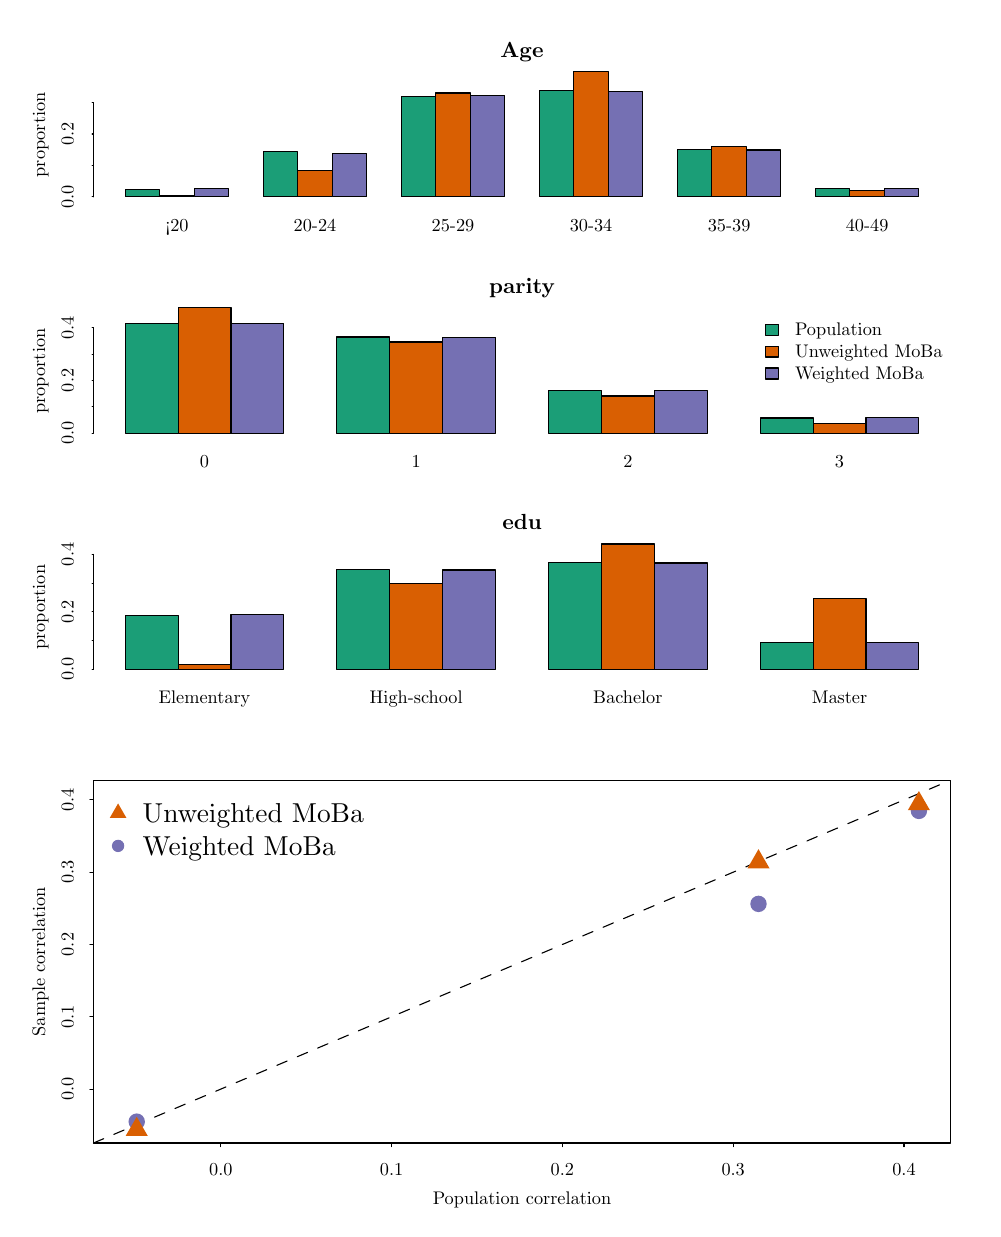
\begin{tikzpicture}[x=1pt,y=1pt]
\definecolor{fillColor}{RGB}{255,255,255}
\path[use as bounding box,fill=fillColor,fill opacity=0.00] (0,0) rectangle (341.43,426.79);
\begin{scope}
\path[clip] (  0.00,341.43) rectangle (341.43,426.79);
\definecolor{drawColor}{RGB}{0,0,0}
\definecolor{fillColor}{RGB}{27,158,119}

\path[draw=drawColor,line width= 0.4pt,line join=round,line cap=round,fill=fillColor] ( 35.23,365.65) rectangle ( 47.70,368.25);
\definecolor{fillColor}{RGB}{217,95,2}

\path[draw=drawColor,line width= 0.4pt,line join=round,line cap=round,fill=fillColor] ( 47.70,365.65) rectangle ( 60.17,366.30);
\definecolor{fillColor}{RGB}{117,112,179}

\path[draw=drawColor,line width= 0.4pt,line join=round,line cap=round,fill=fillColor] ( 60.17,365.65) rectangle ( 72.64,368.54);
\definecolor{fillColor}{RGB}{27,158,119}

\path[draw=drawColor,line width= 0.4pt,line join=round,line cap=round,fill=fillColor] ( 85.11,365.65) rectangle ( 97.58,382.00);
\definecolor{fillColor}{RGB}{217,95,2}

\path[draw=drawColor,line width= 0.4pt,line join=round,line cap=round,fill=fillColor] ( 97.58,365.65) rectangle (110.05,375.24);
\definecolor{fillColor}{RGB}{117,112,179}

\path[draw=drawColor,line width= 0.4pt,line join=round,line cap=round,fill=fillColor] (110.05,365.65) rectangle (122.52,381.42);
\definecolor{fillColor}{RGB}{27,158,119}

\path[draw=drawColor,line width= 0.4pt,line join=round,line cap=round,fill=fillColor] (134.99,365.65) rectangle (147.46,401.98);
\definecolor{fillColor}{RGB}{217,95,2}

\path[draw=drawColor,line width= 0.4pt,line join=round,line cap=round,fill=fillColor] (147.46,365.65) rectangle (159.93,403.17);
\definecolor{fillColor}{RGB}{117,112,179}

\path[draw=drawColor,line width= 0.4pt,line join=round,line cap=round,fill=fillColor] (159.93,365.65) rectangle (172.40,402.35);
\definecolor{fillColor}{RGB}{27,158,119}

\path[draw=drawColor,line width= 0.4pt,line join=round,line cap=round,fill=fillColor] (184.87,365.65) rectangle (197.34,403.95);
\definecolor{fillColor}{RGB}{217,95,2}

\path[draw=drawColor,line width= 0.4pt,line join=round,line cap=round,fill=fillColor] (197.34,365.65) rectangle (209.81,410.95);
\definecolor{fillColor}{RGB}{117,112,179}

\path[draw=drawColor,line width= 0.4pt,line join=round,line cap=round,fill=fillColor] (209.81,365.65) rectangle (222.28,403.87);
\definecolor{fillColor}{RGB}{27,158,119}

\path[draw=drawColor,line width= 0.4pt,line join=round,line cap=round,fill=fillColor] (234.75,365.65) rectangle (247.22,382.67);
\definecolor{fillColor}{RGB}{217,95,2}

\path[draw=drawColor,line width= 0.4pt,line join=round,line cap=round,fill=fillColor] (247.22,365.65) rectangle (259.69,383.70);
\definecolor{fillColor}{RGB}{117,112,179}

\path[draw=drawColor,line width= 0.4pt,line join=round,line cap=round,fill=fillColor] (259.69,365.65) rectangle (272.16,382.60);
\definecolor{fillColor}{RGB}{27,158,119}

\path[draw=drawColor,line width= 0.4pt,line join=round,line cap=round,fill=fillColor] (284.63,365.65) rectangle (297.10,368.54);
\definecolor{fillColor}{RGB}{217,95,2}

\path[draw=drawColor,line width= 0.4pt,line join=round,line cap=round,fill=fillColor] (297.10,365.65) rectangle (309.57,368.03);
\definecolor{fillColor}{RGB}{117,112,179}

\path[draw=drawColor,line width= 0.4pt,line join=round,line cap=round,fill=fillColor] (309.57,365.65) rectangle (322.04,368.61);
\end{scope}
\begin{scope}
\path[clip] (  0.00,  0.00) rectangle (341.43,426.79);
\definecolor{drawColor}{RGB}{0,0,0}

\node[text=drawColor,anchor=base,inner sep=0pt, outer sep=0pt, scale=  0.66] at ( 53.94,353.31) {<20};

\node[text=drawColor,anchor=base,inner sep=0pt, outer sep=0pt, scale=  0.66] at (103.82,353.31) {20-24};

\node[text=drawColor,anchor=base,inner sep=0pt, outer sep=0pt, scale=  0.66] at (153.70,353.31) {25-29};

\node[text=drawColor,anchor=base,inner sep=0pt, outer sep=0pt, scale=  0.66] at (203.58,353.31) {30-34};

\node[text=drawColor,anchor=base,inner sep=0pt, outer sep=0pt, scale=  0.66] at (253.46,353.31) {35-39};

\node[text=drawColor,anchor=base,inner sep=0pt, outer sep=0pt, scale=  0.66] at (303.34,353.31) {40-49};
\end{scope}
\begin{scope}
\path[clip] (  0.00,341.43) rectangle (341.43,426.79);
\definecolor{drawColor}{RGB}{0,0,0}

\node[text=drawColor,anchor=base,inner sep=0pt, outer sep=0pt, scale=  0.79] at (178.64,416.14) {\bfseries Age};

\node[text=drawColor,rotate= 90.00,anchor=base,inner sep=0pt, outer sep=0pt, scale=  0.66] at (  6.34,388.07) {proportion};
\end{scope}
\begin{scope}
\path[clip] (  0.00,  0.00) rectangle (341.43,426.79);
\definecolor{drawColor}{RGB}{0,0,0}

\path[draw=drawColor,line width= 0.4pt,line join=round,line cap=round] ( 23.76,365.65) -- ( 23.76,399.70);

\path[draw=drawColor,line width= 0.4pt,line join=round,line cap=round] ( 23.76,365.65) -- ( 23.30,365.65);

\path[draw=drawColor,line width= 0.4pt,line join=round,line cap=round] ( 23.76,377.00) -- ( 23.30,377.00);

\path[draw=drawColor,line width= 0.4pt,line join=round,line cap=round] ( 23.76,388.35) -- ( 23.30,388.35);

\path[draw=drawColor,line width= 0.4pt,line join=round,line cap=round] ( 23.76,399.70) -- ( 23.30,399.70);

\node[text=drawColor,rotate= 90.00,anchor=base,inner sep=0pt, outer sep=0pt, scale=  0.66] at ( 16.63,365.65) {0.0};

\node[text=drawColor,rotate= 90.00,anchor=base,inner sep=0pt, outer sep=0pt, scale=  0.66] at ( 16.63,388.35) {0.2};
\end{scope}
\begin{scope}
\path[clip] (  0.00,256.07) rectangle (341.43,341.43);
\definecolor{drawColor}{RGB}{0,0,0}
\definecolor{fillColor}{RGB}{27,158,119}

\path[draw=drawColor,line width= 0.4pt,line join=round,line cap=round,fill=fillColor] ( 35.23,280.29) rectangle ( 54.35,320.00);
\definecolor{fillColor}{RGB}{217,95,2}

\path[draw=drawColor,line width= 0.4pt,line join=round,line cap=round,fill=fillColor] ( 54.35,280.29) rectangle ( 73.47,325.59);
\definecolor{fillColor}{RGB}{117,112,179}

\path[draw=drawColor,line width= 0.4pt,line join=round,line cap=round,fill=fillColor] ( 73.47,280.29) rectangle ( 92.59,319.96);
\definecolor{fillColor}{RGB}{27,158,119}

\path[draw=drawColor,line width= 0.4pt,line join=round,line cap=round,fill=fillColor] (111.71,280.29) rectangle (130.84,315.00);
\definecolor{fillColor}{RGB}{217,95,2}

\path[draw=drawColor,line width= 0.4pt,line join=round,line cap=round,fill=fillColor] (130.84,280.29) rectangle (149.96,313.19);
\definecolor{fillColor}{RGB}{117,112,179}

\path[draw=drawColor,line width= 0.4pt,line join=round,line cap=round,fill=fillColor] (149.96,280.29) rectangle (169.08,314.87);
\definecolor{fillColor}{RGB}{27,158,119}

\path[draw=drawColor,line width= 0.4pt,line join=round,line cap=round,fill=fillColor] (188.20,280.29) rectangle (207.32,295.59);
\definecolor{fillColor}{RGB}{217,95,2}

\path[draw=drawColor,line width= 0.4pt,line join=round,line cap=round,fill=fillColor] (207.32,280.29) rectangle (226.44,293.68);
\definecolor{fillColor}{RGB}{117,112,179}

\path[draw=drawColor,line width= 0.4pt,line join=round,line cap=round,fill=fillColor] (226.44,280.29) rectangle (245.56,295.67);
\definecolor{fillColor}{RGB}{27,158,119}

\path[draw=drawColor,line width= 0.4pt,line join=round,line cap=round,fill=fillColor] (264.68,280.29) rectangle (283.80,285.74);
\definecolor{fillColor}{RGB}{217,95,2}

\path[draw=drawColor,line width= 0.4pt,line join=round,line cap=round,fill=fillColor] (283.80,280.29) rectangle (302.92,283.88);
\definecolor{fillColor}{RGB}{117,112,179}

\path[draw=drawColor,line width= 0.4pt,line join=round,line cap=round,fill=fillColor] (302.92,280.29) rectangle (322.04,285.84);
\end{scope}
\begin{scope}
\path[clip] (  0.00,  0.00) rectangle (341.43,426.79);
\definecolor{drawColor}{RGB}{0,0,0}

\node[text=drawColor,anchor=base,inner sep=0pt, outer sep=0pt, scale=  0.66] at ( 63.91,267.95) {0};

\node[text=drawColor,anchor=base,inner sep=0pt, outer sep=0pt, scale=  0.66] at (140.40,267.95) {1};

\node[text=drawColor,anchor=base,inner sep=0pt, outer sep=0pt, scale=  0.66] at (216.88,267.95) {2};

\node[text=drawColor,anchor=base,inner sep=0pt, outer sep=0pt, scale=  0.66] at (293.36,267.95) {3};
\end{scope}
\begin{scope}
\path[clip] (  0.00,256.07) rectangle (341.43,341.43);
\definecolor{drawColor}{RGB}{0,0,0}

\node[text=drawColor,anchor=base,inner sep=0pt, outer sep=0pt, scale=  0.79] at (178.64,330.78) {\bfseries parity};

\node[text=drawColor,rotate= 90.00,anchor=base,inner sep=0pt, outer sep=0pt, scale=  0.66] at (  6.34,302.71) {proportion};
\end{scope}
\begin{scope}
\path[clip] (  0.00,  0.00) rectangle (341.43,426.79);
\definecolor{drawColor}{RGB}{0,0,0}

\path[draw=drawColor,line width= 0.4pt,line join=round,line cap=round] ( 23.76,280.29) -- ( 23.76,318.36);

\path[draw=drawColor,line width= 0.4pt,line join=round,line cap=round] ( 23.76,280.29) -- ( 23.30,280.29);

\path[draw=drawColor,line width= 0.4pt,line join=round,line cap=round] ( 23.76,289.81) -- ( 23.30,289.81);

\path[draw=drawColor,line width= 0.4pt,line join=round,line cap=round] ( 23.76,299.32) -- ( 23.30,299.32);

\path[draw=drawColor,line width= 0.4pt,line join=round,line cap=round] ( 23.76,308.84) -- ( 23.30,308.84);

\path[draw=drawColor,line width= 0.4pt,line join=round,line cap=round] ( 23.76,318.36) -- ( 23.30,318.36);

\node[text=drawColor,rotate= 90.00,anchor=base,inner sep=0pt, outer sep=0pt, scale=  0.66] at ( 16.63,280.29) {0.0};

\node[text=drawColor,rotate= 90.00,anchor=base,inner sep=0pt, outer sep=0pt, scale=  0.66] at ( 16.63,299.32) {0.2};

\node[text=drawColor,rotate= 90.00,anchor=base,inner sep=0pt, outer sep=0pt, scale=  0.66] at ( 16.63,318.36) {0.4};
\end{scope}
\begin{scope}
\path[clip] ( 23.76,279.83) rectangle (333.51,325.59);
\definecolor{drawColor}{RGB}{0,0,0}
\definecolor{fillColor}{RGB}{27,158,119}

\path[draw=drawColor,line width= 0.4pt,line join=round,line cap=round,fill=fillColor] (266.61,319.65) rectangle (271.36,315.69);
\definecolor{fillColor}{RGB}{217,95,2}

\path[draw=drawColor,line width= 0.4pt,line join=round,line cap=round,fill=fillColor] (266.61,311.73) rectangle (271.36,307.77);
\definecolor{fillColor}{RGB}{117,112,179}

\path[draw=drawColor,line width= 0.4pt,line join=round,line cap=round,fill=fillColor] (266.61,303.81) rectangle (271.36,299.85);

\node[text=drawColor,anchor=base west,inner sep=0pt, outer sep=0pt, scale=  0.66] at (277.30,315.40) {Population};

\node[text=drawColor,anchor=base west,inner sep=0pt, outer sep=0pt, scale=  0.66] at (277.30,307.48) {Unweighted MoBa};

\node[text=drawColor,anchor=base west,inner sep=0pt, outer sep=0pt, scale=  0.66] at (277.30,299.56) {Weighted MoBa};
\end{scope}
\begin{scope}
\path[clip] (  0.00,170.72) rectangle (341.43,256.07);
\definecolor{drawColor}{RGB}{0,0,0}
\definecolor{fillColor}{RGB}{27,158,119}

\path[draw=drawColor,line width= 0.4pt,line join=round,line cap=round,fill=fillColor] ( 35.23,194.93) rectangle ( 54.35,214.38);
\definecolor{fillColor}{RGB}{217,95,2}

\path[draw=drawColor,line width= 0.4pt,line join=round,line cap=round,fill=fillColor] ( 54.35,194.93) rectangle ( 73.47,196.73);
\definecolor{fillColor}{RGB}{117,112,179}

\path[draw=drawColor,line width= 0.4pt,line join=round,line cap=round,fill=fillColor] ( 73.47,194.93) rectangle ( 92.59,214.73);
\definecolor{fillColor}{RGB}{27,158,119}

\path[draw=drawColor,line width= 0.4pt,line join=round,line cap=round,fill=fillColor] (111.71,194.93) rectangle (130.84,230.95);
\definecolor{fillColor}{RGB}{217,95,2}

\path[draw=drawColor,line width= 0.4pt,line join=round,line cap=round,fill=fillColor] (130.84,194.93) rectangle (149.96,225.97);
\definecolor{fillColor}{RGB}{117,112,179}

\path[draw=drawColor,line width= 0.4pt,line join=round,line cap=round,fill=fillColor] (149.96,194.93) rectangle (169.08,230.82);
\definecolor{fillColor}{RGB}{27,158,119}

\path[draw=drawColor,line width= 0.4pt,line join=round,line cap=round,fill=fillColor] (188.20,194.93) rectangle (207.32,233.55);
\definecolor{fillColor}{RGB}{217,95,2}

\path[draw=drawColor,line width= 0.4pt,line join=round,line cap=round,fill=fillColor] (207.32,194.93) rectangle (226.44,240.23);
\definecolor{fillColor}{RGB}{117,112,179}

\path[draw=drawColor,line width= 0.4pt,line join=round,line cap=round,fill=fillColor] (226.44,194.93) rectangle (245.56,233.35);
\definecolor{fillColor}{RGB}{27,158,119}

\path[draw=drawColor,line width= 0.4pt,line join=round,line cap=round,fill=fillColor] (264.68,194.93) rectangle (283.80,204.61);
\definecolor{fillColor}{RGB}{217,95,2}

\path[draw=drawColor,line width= 0.4pt,line join=round,line cap=round,fill=fillColor] (283.80,194.93) rectangle (302.92,220.56);
\definecolor{fillColor}{RGB}{117,112,179}

\path[draw=drawColor,line width= 0.4pt,line join=round,line cap=round,fill=fillColor] (302.92,194.93) rectangle (322.04,204.60);
\end{scope}
\begin{scope}
\path[clip] (  0.00,  0.00) rectangle (341.43,426.79);
\definecolor{drawColor}{RGB}{0,0,0}

\node[text=drawColor,anchor=base,inner sep=0pt, outer sep=0pt, scale=  0.66] at ( 63.91,182.60) {Elementary};

\node[text=drawColor,anchor=base,inner sep=0pt, outer sep=0pt, scale=  0.66] at (140.40,182.60) {High-school};

\node[text=drawColor,anchor=base,inner sep=0pt, outer sep=0pt, scale=  0.66] at (216.88,182.60) {Bachelor};

\node[text=drawColor,anchor=base,inner sep=0pt, outer sep=0pt, scale=  0.66] at (293.36,182.60) {Master};
\end{scope}
\begin{scope}
\path[clip] (  0.00,170.72) rectangle (341.43,256.07);
\definecolor{drawColor}{RGB}{0,0,0}

\node[text=drawColor,anchor=base,inner sep=0pt, outer sep=0pt, scale=  0.79] at (178.64,245.42) {\bfseries edu};

\node[text=drawColor,rotate= 90.00,anchor=base,inner sep=0pt, outer sep=0pt, scale=  0.66] at (  6.34,217.36) {proportion};
\end{scope}
\begin{scope}
\path[clip] (  0.00,  0.00) rectangle (341.43,426.79);
\definecolor{drawColor}{RGB}{0,0,0}

\path[draw=drawColor,line width= 0.4pt,line join=round,line cap=round] ( 23.76,194.93) -- ( 23.76,236.44);

\path[draw=drawColor,line width= 0.4pt,line join=round,line cap=round] ( 23.76,194.93) -- ( 23.30,194.93);

\path[draw=drawColor,line width= 0.4pt,line join=round,line cap=round] ( 23.76,205.31) -- ( 23.30,205.31);

\path[draw=drawColor,line width= 0.4pt,line join=round,line cap=round] ( 23.76,215.68) -- ( 23.30,215.68);

\path[draw=drawColor,line width= 0.4pt,line join=round,line cap=round] ( 23.76,226.06) -- ( 23.30,226.06);

\path[draw=drawColor,line width= 0.4pt,line join=round,line cap=round] ( 23.76,236.44) -- ( 23.30,236.44);

\node[text=drawColor,rotate= 90.00,anchor=base,inner sep=0pt, outer sep=0pt, scale=  0.66] at ( 16.63,194.93) {0.0};

\node[text=drawColor,rotate= 90.00,anchor=base,inner sep=0pt, outer sep=0pt, scale=  0.66] at ( 16.63,215.68) {0.2};

\node[text=drawColor,rotate= 90.00,anchor=base,inner sep=0pt, outer sep=0pt, scale=  0.66] at ( 16.63,236.44) {0.4};
\end{scope}
\begin{scope}
\path[clip] (  0.00,  0.00) rectangle (341.43,426.79);
\definecolor{drawColor}{RGB}{0,0,0}

\path[draw=drawColor,line width= 0.4pt,line join=round,line cap=round] ( 69.79, 23.76) -- (316.66, 23.76);

\path[draw=drawColor,line width= 0.4pt,line join=round,line cap=round] ( 69.79, 23.76) -- ( 69.79, 22.45);

\path[draw=drawColor,line width= 0.4pt,line join=round,line cap=round] (131.51, 23.76) -- (131.51, 22.45);

\path[draw=drawColor,line width= 0.4pt,line join=round,line cap=round] (193.22, 23.76) -- (193.22, 22.45);

\path[draw=drawColor,line width= 0.4pt,line join=round,line cap=round] (254.94, 23.76) -- (254.94, 22.45);

\path[draw=drawColor,line width= 0.4pt,line join=round,line cap=round] (316.66, 23.76) -- (316.66, 22.45);

\node[text=drawColor,anchor=base,inner sep=0pt, outer sep=0pt, scale=  0.66] at ( 69.79, 11.88) {0.0};

\node[text=drawColor,anchor=base,inner sep=0pt, outer sep=0pt, scale=  0.66] at (131.51, 11.88) {0.1};

\node[text=drawColor,anchor=base,inner sep=0pt, outer sep=0pt, scale=  0.66] at (193.22, 11.88) {0.2};

\node[text=drawColor,anchor=base,inner sep=0pt, outer sep=0pt, scale=  0.66] at (254.94, 11.88) {0.3};

\node[text=drawColor,anchor=base,inner sep=0pt, outer sep=0pt, scale=  0.66] at (316.66, 11.88) {0.4};

\path[draw=drawColor,line width= 0.4pt,line join=round,line cap=round] ( 23.76, 43.25) -- ( 23.76,147.74);

\path[draw=drawColor,line width= 0.4pt,line join=round,line cap=round] ( 23.76, 43.25) -- ( 22.45, 43.25);

\path[draw=drawColor,line width= 0.4pt,line join=round,line cap=round] ( 23.76, 69.37) -- ( 22.45, 69.37);

\path[draw=drawColor,line width= 0.4pt,line join=round,line cap=round] ( 23.76, 95.49) -- ( 22.45, 95.49);

\path[draw=drawColor,line width= 0.4pt,line join=round,line cap=round] ( 23.76,121.62) -- ( 22.45,121.62);

\path[draw=drawColor,line width= 0.4pt,line join=round,line cap=round] ( 23.76,147.74) -- ( 22.45,147.74);

\node[text=drawColor,rotate= 90.00,anchor=base,inner sep=0pt, outer sep=0pt, scale=  0.66] at ( 16.63, 43.25) {0.0};

\node[text=drawColor,rotate= 90.00,anchor=base,inner sep=0pt, outer sep=0pt, scale=  0.66] at ( 16.63, 69.37) {0.1};

\node[text=drawColor,rotate= 90.00,anchor=base,inner sep=0pt, outer sep=0pt, scale=  0.66] at ( 16.63, 95.49) {0.2};

\node[text=drawColor,rotate= 90.00,anchor=base,inner sep=0pt, outer sep=0pt, scale=  0.66] at ( 16.63,121.62) {0.3};

\node[text=drawColor,rotate= 90.00,anchor=base,inner sep=0pt, outer sep=0pt, scale=  0.66] at ( 16.63,147.74) {0.4};

\path[draw=drawColor,line width= 0.4pt,line join=round,line cap=round] ( 23.76, 23.76) --
	(333.51, 23.76) --
	(333.51,154.88) --
	( 23.76,154.88) --
	( 23.76, 23.76);
\end{scope}
\begin{scope}
\path[clip] (  0.00,  0.00) rectangle (341.43,170.72);
\definecolor{drawColor}{RGB}{0,0,0}

\node[text=drawColor,anchor=base,inner sep=0pt, outer sep=0pt, scale=  0.66] at (178.64,  1.58) {Population correlation};

\node[text=drawColor,rotate= 90.00,anchor=base,inner sep=0pt, outer sep=0pt, scale=  0.66] at (  6.34, 89.32) {Sample correlation};
\end{scope}
\begin{scope}
\path[clip] ( 23.76, 23.76) rectangle (333.51,154.88);
\definecolor{drawColor}{RGB}{0,0,0}

\path[draw=drawColor,line width= 0.4pt,dash pattern=on 4pt off 4pt ,line join=round,line cap=round] ( 23.76, 23.76) -- (333.51,154.88);
\definecolor{fillColor}{RGB}{117,112,179}

\path[fill=fillColor] (264.08,110.17) circle (  2.97);

\path[fill=fillColor] ( 39.40, 31.48) circle (  2.97);

\path[fill=fillColor] (322.04,143.77) circle (  2.97);
\definecolor{fillColor}{RGB}{217,95,2}

\path[fill=fillColor] (264.08,129.93) --
	(268.08,123.01) --
	(260.09,123.01) --
	cycle;

\path[fill=fillColor] ( 39.40, 33.23) --
	( 43.40, 26.31) --
	( 35.40, 26.31) --
	cycle;

\path[fill=fillColor] (322.04,150.94) --
	(326.04,144.01) --
	(318.04,144.01) --
	cycle;

\path[fill=fillColor] ( 32.67,146.46) --
	( 35.67,141.26) --
	( 29.67,141.26) --
	cycle;
\definecolor{fillColor}{RGB}{117,112,179}

\path[fill=fillColor] ( 32.67,131.12) circle (  2.23);

\node[text=drawColor,anchor=base west,inner sep=0pt, outer sep=0pt, scale=  0.99] at ( 41.58,139.59) {Unweighted MoBa};

\node[text=drawColor,anchor=base west,inner sep=0pt, outer sep=0pt, scale=  0.99] at ( 41.58,127.71) {Weighted MoBa};
\end{scope}
\end{tikzpicture}
	
	\caption{Balance of target population and study samples: Marginal distributions of and correlation between selection variables are identical after IPP weighting, but not before}
	\label{fig:IPWbalance}
\end{figure}



\begin{figure}[H]
	\adjustbox{width=\textwidth}{
		\centering % Created by tikzDevice version 0.12 on 2019-02-08 07:26:59
% !TEX encoding = UTF-8 Unicode
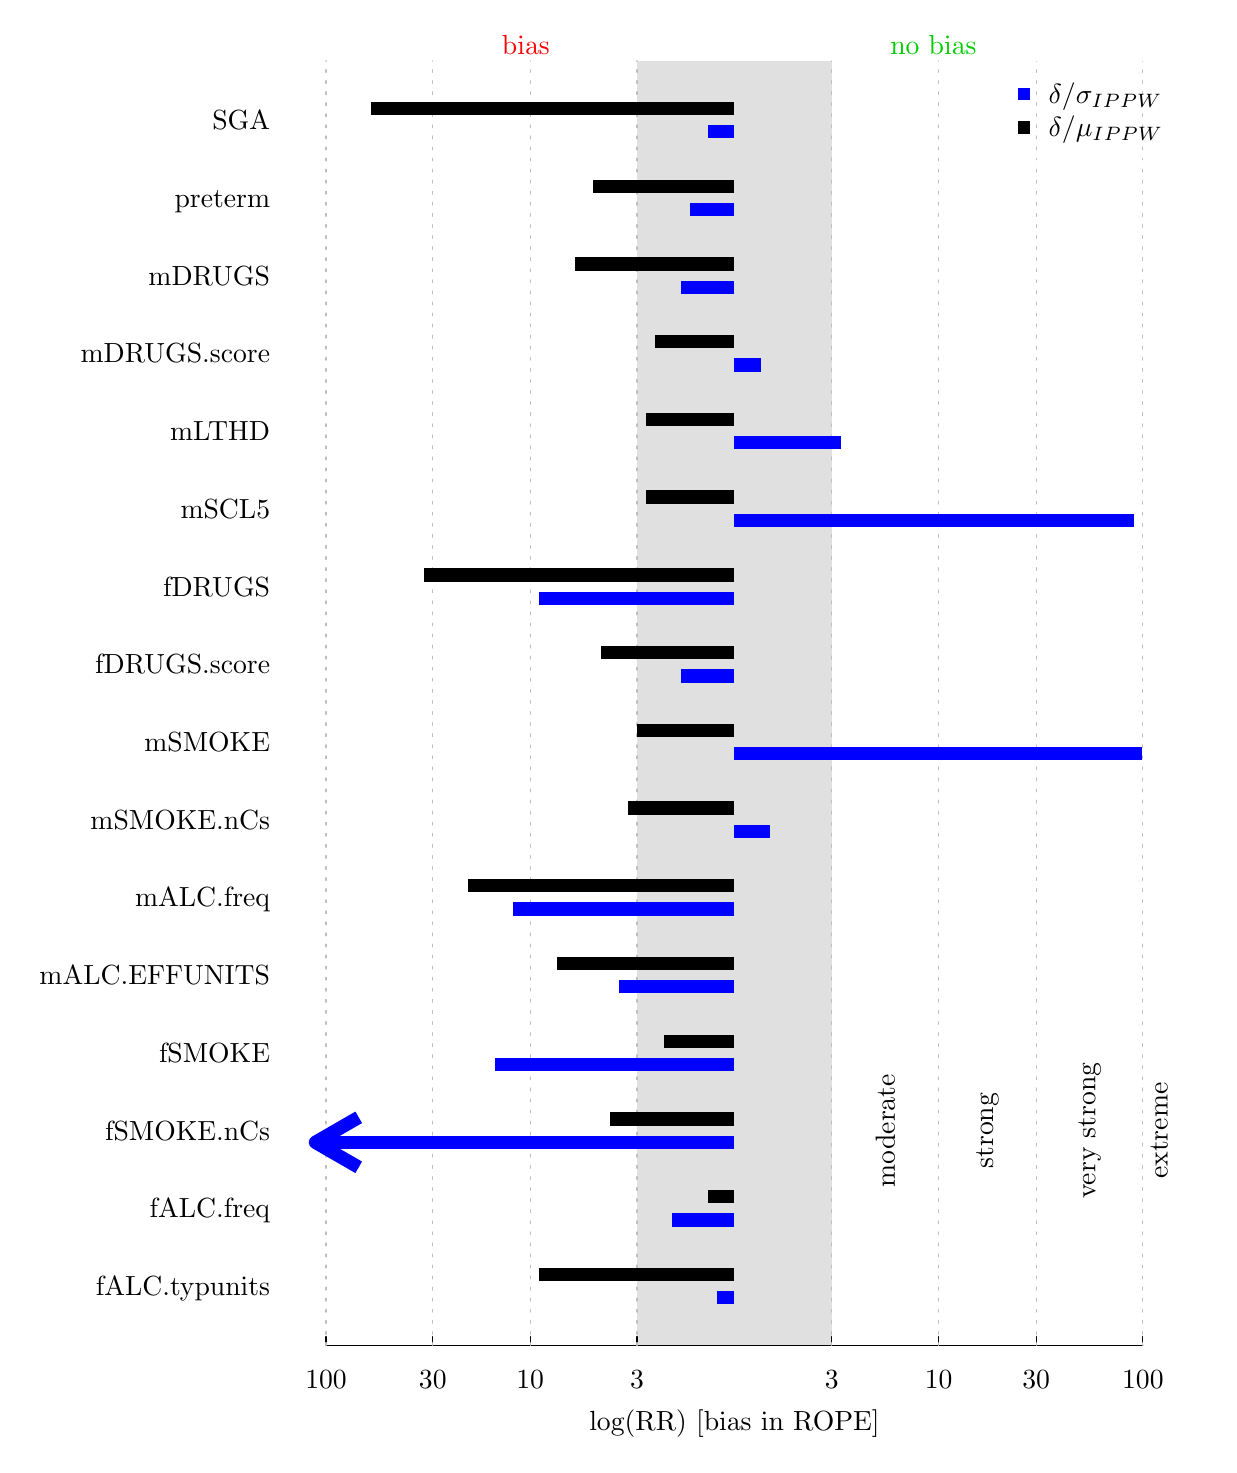
\begin{tikzpicture}[x=1pt,y=1pt]
\definecolor{fillColor}{RGB}{255,255,255}
\path[use as bounding box,fill=fillColor,fill opacity=0.00] (0,0) rectangle (426.79,512.15);
\begin{scope}
\path[clip] (  0.00,  0.00) rectangle (426.79,512.15);
\definecolor{drawColor}{RGB}{0,0,0}

\node[text=drawColor,anchor=base,inner sep=0pt, outer sep=0pt, scale=  1.00] at (255.40,  5.40) {log(RR) [bias in ROPE]};
\end{scope}
\begin{scope}
\path[clip] ( 96.00, 36.00) rectangle (414.79,500.15);
\definecolor{fillColor}{gray}{0.88}

\path[fill=fillColor] (220.19, 36.00) rectangle (290.60,500.15);
\end{scope}
\begin{scope}
\path[clip] (  0.00,  0.00) rectangle (426.79,512.15);
\definecolor{drawColor}{RGB}{0,0,0}

\path[draw=drawColor,line width= 0.4pt,line join=round,line cap=round] (107.81, 36.00) -- (402.98, 36.00);

\path[draw=drawColor,line width= 0.4pt,line join=round,line cap=round] (107.81, 36.00) -- (107.81, 39.19);

\path[draw=drawColor,line width= 0.4pt,line join=round,line cap=round] (146.39, 36.00) -- (146.39, 39.19);

\path[draw=drawColor,line width= 0.4pt,line join=round,line cap=round] (181.60, 36.00) -- (181.60, 39.19);

\path[draw=drawColor,line width= 0.4pt,line join=round,line cap=round] (220.19, 36.00) -- (220.19, 39.19);

\path[draw=drawColor,line width= 0.4pt,line join=round,line cap=round] (290.60, 36.00) -- (290.60, 39.19);

\path[draw=drawColor,line width= 0.4pt,line join=round,line cap=round] (329.19, 36.00) -- (329.19, 39.19);

\path[draw=drawColor,line width= 0.4pt,line join=round,line cap=round] (364.40, 36.00) -- (364.40, 39.19);

\path[draw=drawColor,line width= 0.4pt,line join=round,line cap=round] (402.98, 36.00) -- (402.98, 39.19);

\node[text=drawColor,anchor=base,inner sep=0pt, outer sep=0pt, scale=  1.00] at (107.81, 20.40) {100};

\node[text=drawColor,anchor=base,inner sep=0pt, outer sep=0pt, scale=  1.00] at (146.39, 20.40) {30};

\node[text=drawColor,anchor=base,inner sep=0pt, outer sep=0pt, scale=  1.00] at (181.60, 20.40) {10};

\node[text=drawColor,anchor=base,inner sep=0pt, outer sep=0pt, scale=  1.00] at (220.19, 20.40) {3};

\node[text=drawColor,anchor=base,inner sep=0pt, outer sep=0pt, scale=  1.00] at (290.60, 20.40) {3};

\node[text=drawColor,anchor=base,inner sep=0pt, outer sep=0pt, scale=  1.00] at (329.19, 20.40) {10};

\node[text=drawColor,anchor=base,inner sep=0pt, outer sep=0pt, scale=  1.00] at (364.40, 20.40) {30};

\node[text=drawColor,anchor=base,inner sep=0pt, outer sep=0pt, scale=  1.00] at (402.98, 20.40) {100};
\end{scope}
\begin{scope}
\path[clip] ( 96.00, 36.00) rectangle (414.79,500.15);
\definecolor{drawColor}{RGB}{190,190,190}

\path[draw=drawColor,line width= 0.4pt,dash pattern=on 1pt off 3pt ,line join=round,line cap=round] (107.81, 36.00) -- (107.81,500.15);

\path[draw=drawColor,line width= 0.4pt,dash pattern=on 1pt off 3pt ,line join=round,line cap=round] (146.39, 36.00) -- (146.39,500.15);

\path[draw=drawColor,line width= 0.4pt,dash pattern=on 1pt off 3pt ,line join=round,line cap=round] (181.60, 36.00) -- (181.60,500.15);

\path[draw=drawColor,line width= 0.4pt,dash pattern=on 1pt off 3pt ,line join=round,line cap=round] (220.19, 36.00) -- (220.19,500.15);

\path[draw=drawColor,line width= 0.4pt,dash pattern=on 1pt off 3pt ,line join=round,line cap=round] (290.60, 36.00) -- (290.60,500.15);

\path[draw=drawColor,line width= 0.4pt,dash pattern=on 1pt off 3pt ,line join=round,line cap=round] (329.19, 36.00) -- (329.19,500.15);

\path[draw=drawColor,line width= 0.4pt,dash pattern=on 1pt off 3pt ,line join=round,line cap=round] (364.40, 36.00) -- (364.40,500.15);

\path[draw=drawColor,line width= 0.4pt,dash pattern=on 1pt off 3pt ,line join=round,line cap=round] (402.98, 36.00) -- (402.98,500.15);
\end{scope}
\begin{scope}
\path[clip] (  0.00,  0.00) rectangle (426.79,512.15);
\definecolor{drawColor}{RGB}{255,0,0}

\node[text=drawColor,anchor=base,inner sep=0pt, outer sep=0pt, scale=  1.00] at (180.02,502.55) {bias};
\definecolor{drawColor}{RGB}{0,205,0}

\node[text=drawColor,anchor=base east,inner sep=0pt, outer sep=0pt, scale=  1.00] at (342.88,502.55) {no bias};
\definecolor{drawColor}{RGB}{0,0,0}

\node[text=drawColor,anchor=base east,inner sep=0pt, outer sep=0pt, scale=  1.00] at ( 87.60, 53.96) {fALC.typunits};

\node[text=drawColor,anchor=base east,inner sep=0pt, outer sep=0pt, scale=  1.00] at ( 87.60, 82.05) {fALC.freq};

\node[text=drawColor,anchor=base east,inner sep=0pt, outer sep=0pt, scale=  1.00] at ( 87.60,110.14) {fSMOKE.nCs};

\node[text=drawColor,anchor=base east,inner sep=0pt, outer sep=0pt, scale=  1.00] at ( 87.60,138.23) {fSMOKE};

\node[text=drawColor,anchor=base east,inner sep=0pt, outer sep=0pt, scale=  1.00] at ( 87.60,166.32) {mALC.EFFUNITS};

\node[text=drawColor,anchor=base east,inner sep=0pt, outer sep=0pt, scale=  1.00] at ( 87.60,194.41) {mALC.freq};

\node[text=drawColor,anchor=base east,inner sep=0pt, outer sep=0pt, scale=  1.00] at ( 87.60,222.50) {mSMOKE.nCs};

\node[text=drawColor,anchor=base east,inner sep=0pt, outer sep=0pt, scale=  1.00] at ( 87.60,250.59) {mSMOKE};

\node[text=drawColor,anchor=base east,inner sep=0pt, outer sep=0pt, scale=  1.00] at ( 87.60,278.68) {fDRUGS.score};

\node[text=drawColor,anchor=base east,inner sep=0pt, outer sep=0pt, scale=  1.00] at ( 87.60,306.77) {fDRUGS};

\node[text=drawColor,anchor=base east,inner sep=0pt, outer sep=0pt, scale=  1.00] at ( 87.60,334.85) {mSCL5};

\node[text=drawColor,anchor=base east,inner sep=0pt, outer sep=0pt, scale=  1.00] at ( 87.60,362.94) {mLTHD};

\node[text=drawColor,anchor=base east,inner sep=0pt, outer sep=0pt, scale=  1.00] at ( 87.60,391.03) {mDRUGS.score};

\node[text=drawColor,anchor=base east,inner sep=0pt, outer sep=0pt, scale=  1.00] at ( 87.60,419.12) {mDRUGS};

\node[text=drawColor,anchor=base east,inner sep=0pt, outer sep=0pt, scale=  1.00] at ( 87.60,447.21) {preterm};

\node[text=drawColor,anchor=base east,inner sep=0pt, outer sep=0pt, scale=  1.00] at ( 87.60,475.30) {SGA};
\end{scope}
\begin{scope}
\path[clip] ( 96.00, 36.00) rectangle (414.79,500.15);
\definecolor{drawColor}{RGB}{0,0,255}

\path[draw=drawColor,line width= 4.8pt,line join=round] (255.40,474.53) -- (245.78,474.53);

\path[draw=drawColor,line width= 4.8pt,line join=round] (255.40,446.44) -- (239.37,446.44);

\path[draw=drawColor,line width= 4.8pt,line join=round] (255.40,418.35) -- (236.17,418.35);

\path[draw=drawColor,line width= 4.8pt,line join=round] (255.40,390.26) -- (265.01,390.26);

\path[draw=drawColor,line width= 4.8pt,line join=round] (255.40,362.17) -- (293.85,362.17);

\path[draw=drawColor,line width= 4.8pt,line join=round] (255.40,334.08) -- (399.61,334.08);

\path[draw=drawColor,line width= 4.8pt,line join=round] (255.40,306.00) -- (184.89,306.00);

\path[draw=drawColor,line width= 4.8pt,line join=round] (255.40,277.91) -- (236.17,277.91);

\path[draw=drawColor,line width= 4.8pt,line join=round] (255.40,249.82) -- (402.82,249.82);

\path[draw=drawColor,line width= 4.8pt,line join=round] (255.40,221.73) -- (268.22,221.73);

\path[draw=drawColor,line width= 4.8pt,line join=round] (255.40,193.64) -- (175.27,193.64);

\path[draw=drawColor,line width= 4.8pt,line join=round] (255.40,165.55) -- (213.73,165.55);

\path[draw=drawColor,line width= 4.8pt,line join=round] (255.40,137.46) -- (168.86,137.46);

\path[draw=drawColor,line width= 4.8pt,line join=round] (255.40, 81.28) -- (232.96, 81.28);

\path[draw=drawColor,line width= 4.8pt,line join=round] (255.40, 53.19) -- (248.99, 53.19);

\path[draw=drawColor,line width= 4.8pt,line join=round] (255.40,109.37) -- (103.97,109.37);

\path[draw=drawColor,line width= 4.8pt,line join=round] (119.62,118.40) --
	(103.97,109.37) --
	(119.62,100.34);
\definecolor{drawColor}{RGB}{0,0,0}

\path[draw=drawColor,line width= 4.8pt,line join=round] (255.40,482.96) -- (124.00,482.96);

\path[draw=drawColor,line width= 4.8pt,line join=round] (255.40,454.87) -- (204.12,454.87);

\path[draw=drawColor,line width= 4.8pt,line join=round] (255.40,426.78) -- (197.71,426.78);

\path[draw=drawColor,line width= 4.8pt,line join=round] (255.40,398.69) -- (226.55,398.69);

\path[draw=drawColor,line width= 4.8pt,line join=round] (255.40,370.60) -- (223.35,370.60);

\path[draw=drawColor,line width= 4.8pt,line join=round] (255.40,342.51) -- (223.35,342.51);

\path[draw=drawColor,line width= 4.8pt,line join=round] (255.40,314.42) -- (143.23,314.42);

\path[draw=drawColor,line width= 4.8pt,line join=round] (255.40,286.33) -- (207.32,286.33);

\path[draw=drawColor,line width= 4.8pt,line join=round] (255.40,258.24) -- (220.14,258.24);

\path[draw=drawColor,line width= 4.8pt,line join=round] (255.40,230.15) -- (216.94,230.15);

\path[draw=drawColor,line width= 4.8pt,line join=round] (255.40,202.06) -- (159.25,202.06);

\path[draw=drawColor,line width= 4.8pt,line join=round] (255.40,173.98) -- (191.30,173.98);

\path[draw=drawColor,line width= 4.8pt,line join=round] (255.40,145.89) -- (229.76,145.89);

\path[draw=drawColor,line width= 4.8pt,line join=round] (255.40,117.80) -- (210.53,117.80);

\path[draw=drawColor,line width= 4.8pt,line join=round] (255.40, 89.71) -- (245.78, 89.71);

\path[draw=drawColor,line width= 4.8pt,line join=round] (255.40, 61.62) -- (184.89, 61.62);
\end{scope}
\begin{scope}
\path[clip] (  0.00,  0.00) rectangle (426.79,512.15);
\definecolor{drawColor}{RGB}{0,0,0}

\node[text=drawColor,rotate= 90.00,anchor=base,inner sep=0pt, outer sep=0pt, scale=  1.00] at (313.34,113.58) {moderate};

\node[text=drawColor,rotate= 90.00,anchor=base,inner sep=0pt, outer sep=0pt, scale=  1.00] at (348.90,113.58) {strong};

\node[text=drawColor,rotate= 90.00,anchor=base,inner sep=0pt, outer sep=0pt, scale=  1.00] at (385.79,113.58) {very strong};

\node[text=drawColor,rotate= 90.00,anchor=base,inner sep=0pt, outer sep=0pt, scale=  1.00] at (411.96,113.58) {extreme};
\definecolor{drawColor}{RGB}{255,255,255}

\path[draw=drawColor,line width= 0.4pt,line join=round,line cap=round] (350.92,500.15) rectangle (414.79,464.15);
\definecolor{fillColor}{RGB}{0,0,255}

\path[fill=fillColor] (357.67,485.90) --
	(362.17,485.90) --
	(362.17,490.40) --
	(357.67,490.40) --
	cycle;
\definecolor{fillColor}{RGB}{0,0,0}

\path[fill=fillColor] (357.67,473.90) --
	(362.17,473.90) --
	(362.17,478.40) --
	(357.67,478.40) --
	cycle;
\definecolor{drawColor}{RGB}{0,0,0}

\node[text=drawColor,anchor=base west,inner sep=0pt, outer sep=0pt, scale=  1.00] at (368.92,484.71) {$\delta/\sigma_{IPPW}$};

\node[text=drawColor,anchor=base west,inner sep=0pt, outer sep=0pt, scale=  1.00] at (368.92,472.71) {$\delta/\mu_{IPPW}$};
\end{scope}
\end{tikzpicture}

	}
	\caption{Evidence for and against selection bias in an adjusted regression (AR). To obtain a measure of evidence for or against selection bias, we compare how much of the posterior distribution of the difference between the IPPW and AR estimates fall within vs. outside the region of practical equivalence: $log(RR_b) = logit(\int_{-.5}^{.5}\delta)$. Categorization into positive, strong, or very strong evidence is based on \cite{Kass1995-uv}. Standard deviation (mean) standardised bias estimates are shown in in blue (black).} 
	\label{fig:logRRsAR}
\end{figure}

\begin{figure}[H]
	\adjustbox{width=\textwidth}{
		\centering % Created by tikzDevice version 0.12 on 2019-02-08 07:27:37
% !TEX encoding = UTF-8 Unicode
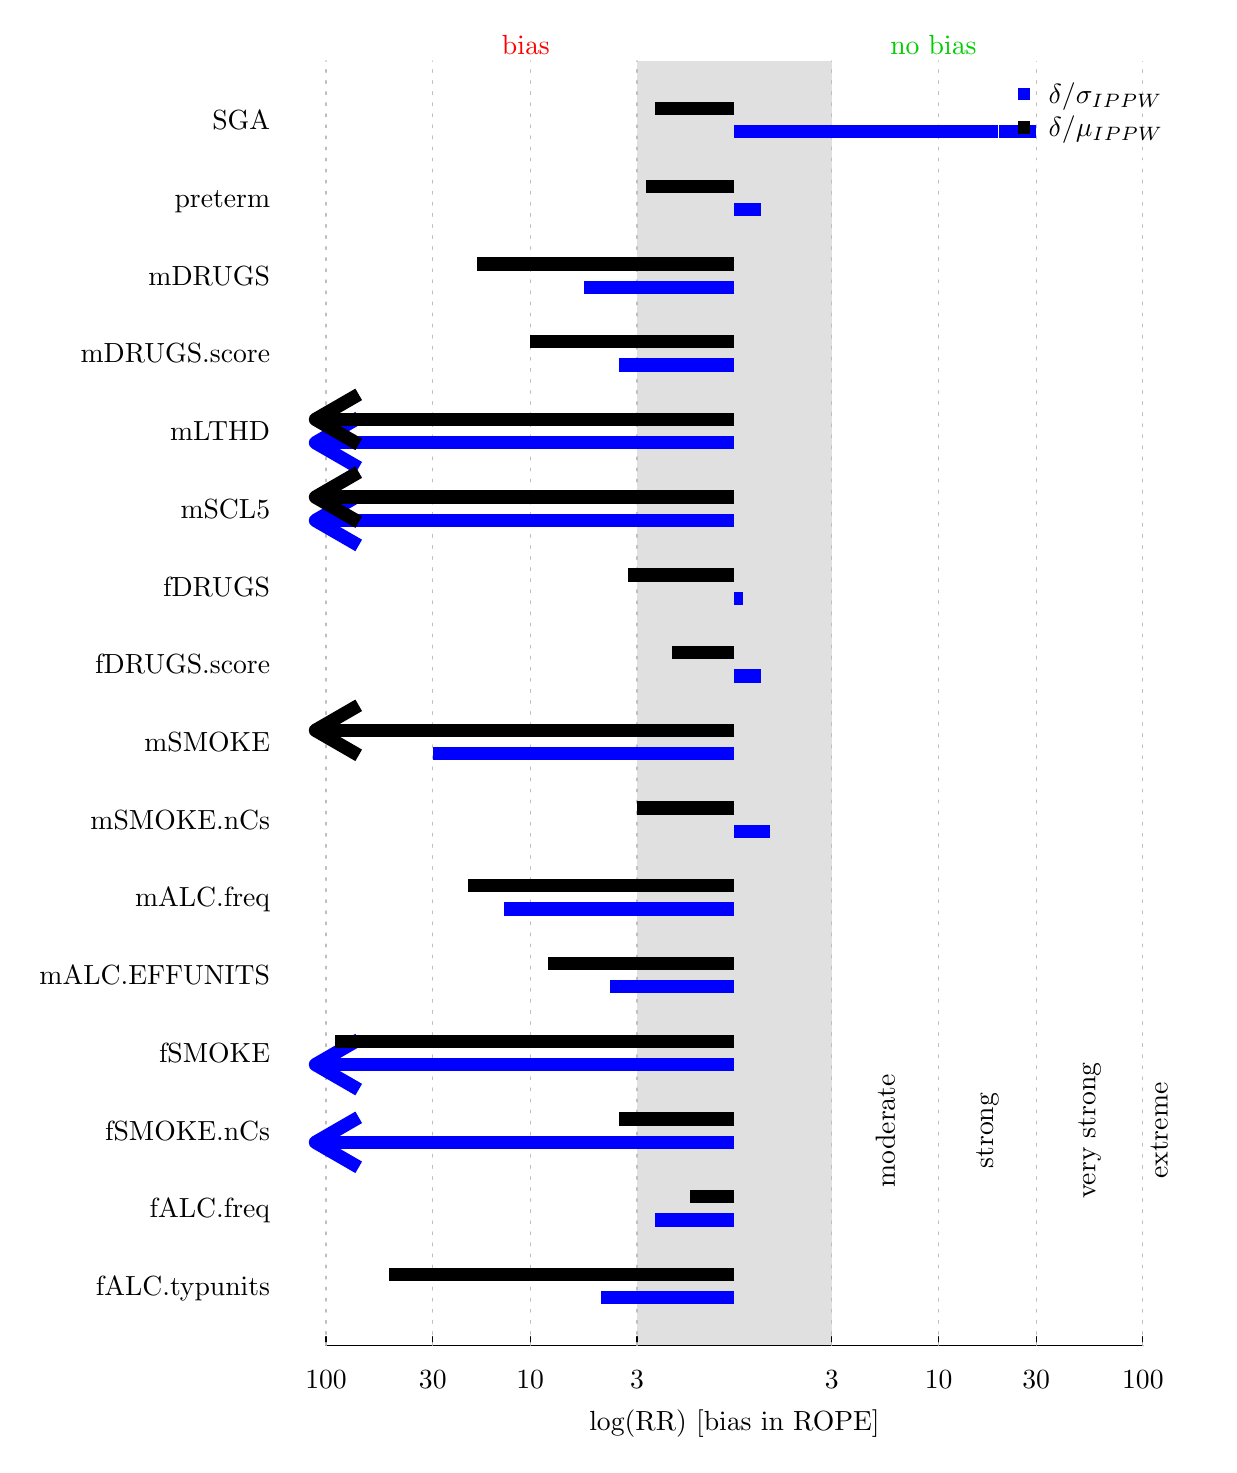
\begin{tikzpicture}[x=1pt,y=1pt]
\definecolor{fillColor}{RGB}{255,255,255}
\path[use as bounding box,fill=fillColor,fill opacity=0.00] (0,0) rectangle (426.79,512.15);
\begin{scope}
\path[clip] (  0.00,  0.00) rectangle (426.79,512.15);
\definecolor{drawColor}{RGB}{0,0,0}

\node[text=drawColor,anchor=base,inner sep=0pt, outer sep=0pt, scale=  1.00] at (255.40,  5.40) {log(RR) [bias in ROPE]};
\end{scope}
\begin{scope}
\path[clip] ( 96.00, 36.00) rectangle (414.79,500.15);
\definecolor{fillColor}{gray}{0.88}

\path[fill=fillColor] (220.19, 36.00) rectangle (290.60,500.15);
\end{scope}
\begin{scope}
\path[clip] (  0.00,  0.00) rectangle (426.79,512.15);
\definecolor{drawColor}{RGB}{0,0,0}

\path[draw=drawColor,line width= 0.4pt,line join=round,line cap=round] (107.81, 36.00) -- (402.98, 36.00);

\path[draw=drawColor,line width= 0.4pt,line join=round,line cap=round] (107.81, 36.00) -- (107.81, 39.19);

\path[draw=drawColor,line width= 0.4pt,line join=round,line cap=round] (146.39, 36.00) -- (146.39, 39.19);

\path[draw=drawColor,line width= 0.4pt,line join=round,line cap=round] (181.60, 36.00) -- (181.60, 39.19);

\path[draw=drawColor,line width= 0.4pt,line join=round,line cap=round] (220.19, 36.00) -- (220.19, 39.19);

\path[draw=drawColor,line width= 0.4pt,line join=round,line cap=round] (290.60, 36.00) -- (290.60, 39.19);

\path[draw=drawColor,line width= 0.4pt,line join=round,line cap=round] (329.19, 36.00) -- (329.19, 39.19);

\path[draw=drawColor,line width= 0.4pt,line join=round,line cap=round] (364.40, 36.00) -- (364.40, 39.19);

\path[draw=drawColor,line width= 0.4pt,line join=round,line cap=round] (402.98, 36.00) -- (402.98, 39.19);

\node[text=drawColor,anchor=base,inner sep=0pt, outer sep=0pt, scale=  1.00] at (107.81, 20.40) {100};

\node[text=drawColor,anchor=base,inner sep=0pt, outer sep=0pt, scale=  1.00] at (146.39, 20.40) {30};

\node[text=drawColor,anchor=base,inner sep=0pt, outer sep=0pt, scale=  1.00] at (181.60, 20.40) {10};

\node[text=drawColor,anchor=base,inner sep=0pt, outer sep=0pt, scale=  1.00] at (220.19, 20.40) {3};

\node[text=drawColor,anchor=base,inner sep=0pt, outer sep=0pt, scale=  1.00] at (290.60, 20.40) {3};

\node[text=drawColor,anchor=base,inner sep=0pt, outer sep=0pt, scale=  1.00] at (329.19, 20.40) {10};

\node[text=drawColor,anchor=base,inner sep=0pt, outer sep=0pt, scale=  1.00] at (364.40, 20.40) {30};

\node[text=drawColor,anchor=base,inner sep=0pt, outer sep=0pt, scale=  1.00] at (402.98, 20.40) {100};
\end{scope}
\begin{scope}
\path[clip] ( 96.00, 36.00) rectangle (414.79,500.15);
\definecolor{drawColor}{RGB}{190,190,190}

\path[draw=drawColor,line width= 0.4pt,dash pattern=on 1pt off 3pt ,line join=round,line cap=round] (107.81, 36.00) -- (107.81,500.15);

\path[draw=drawColor,line width= 0.4pt,dash pattern=on 1pt off 3pt ,line join=round,line cap=round] (146.39, 36.00) -- (146.39,500.15);

\path[draw=drawColor,line width= 0.4pt,dash pattern=on 1pt off 3pt ,line join=round,line cap=round] (181.60, 36.00) -- (181.60,500.15);

\path[draw=drawColor,line width= 0.4pt,dash pattern=on 1pt off 3pt ,line join=round,line cap=round] (220.19, 36.00) -- (220.19,500.15);

\path[draw=drawColor,line width= 0.4pt,dash pattern=on 1pt off 3pt ,line join=round,line cap=round] (290.60, 36.00) -- (290.60,500.15);

\path[draw=drawColor,line width= 0.4pt,dash pattern=on 1pt off 3pt ,line join=round,line cap=round] (329.19, 36.00) -- (329.19,500.15);

\path[draw=drawColor,line width= 0.4pt,dash pattern=on 1pt off 3pt ,line join=round,line cap=round] (364.40, 36.00) -- (364.40,500.15);

\path[draw=drawColor,line width= 0.4pt,dash pattern=on 1pt off 3pt ,line join=round,line cap=round] (402.98, 36.00) -- (402.98,500.15);
\end{scope}
\begin{scope}
\path[clip] (  0.00,  0.00) rectangle (426.79,512.15);
\definecolor{drawColor}{RGB}{255,0,0}

\node[text=drawColor,anchor=base,inner sep=0pt, outer sep=0pt, scale=  1.00] at (180.02,502.55) {bias};
\definecolor{drawColor}{RGB}{0,205,0}

\node[text=drawColor,anchor=base east,inner sep=0pt, outer sep=0pt, scale=  1.00] at (342.88,502.55) {no bias};
\definecolor{drawColor}{RGB}{0,0,0}

\node[text=drawColor,anchor=base east,inner sep=0pt, outer sep=0pt, scale=  1.00] at ( 87.60, 53.96) {fALC.typunits};

\node[text=drawColor,anchor=base east,inner sep=0pt, outer sep=0pt, scale=  1.00] at ( 87.60, 82.05) {fALC.freq};

\node[text=drawColor,anchor=base east,inner sep=0pt, outer sep=0pt, scale=  1.00] at ( 87.60,110.14) {fSMOKE.nCs};

\node[text=drawColor,anchor=base east,inner sep=0pt, outer sep=0pt, scale=  1.00] at ( 87.60,138.23) {fSMOKE};

\node[text=drawColor,anchor=base east,inner sep=0pt, outer sep=0pt, scale=  1.00] at ( 87.60,166.32) {mALC.EFFUNITS};

\node[text=drawColor,anchor=base east,inner sep=0pt, outer sep=0pt, scale=  1.00] at ( 87.60,194.41) {mALC.freq};

\node[text=drawColor,anchor=base east,inner sep=0pt, outer sep=0pt, scale=  1.00] at ( 87.60,222.50) {mSMOKE.nCs};

\node[text=drawColor,anchor=base east,inner sep=0pt, outer sep=0pt, scale=  1.00] at ( 87.60,250.59) {mSMOKE};

\node[text=drawColor,anchor=base east,inner sep=0pt, outer sep=0pt, scale=  1.00] at ( 87.60,278.68) {fDRUGS.score};

\node[text=drawColor,anchor=base east,inner sep=0pt, outer sep=0pt, scale=  1.00] at ( 87.60,306.77) {fDRUGS};

\node[text=drawColor,anchor=base east,inner sep=0pt, outer sep=0pt, scale=  1.00] at ( 87.60,334.85) {mSCL5};

\node[text=drawColor,anchor=base east,inner sep=0pt, outer sep=0pt, scale=  1.00] at ( 87.60,362.94) {mLTHD};

\node[text=drawColor,anchor=base east,inner sep=0pt, outer sep=0pt, scale=  1.00] at ( 87.60,391.03) {mDRUGS.score};

\node[text=drawColor,anchor=base east,inner sep=0pt, outer sep=0pt, scale=  1.00] at ( 87.60,419.12) {mDRUGS};

\node[text=drawColor,anchor=base east,inner sep=0pt, outer sep=0pt, scale=  1.00] at ( 87.60,447.21) {preterm};

\node[text=drawColor,anchor=base east,inner sep=0pt, outer sep=0pt, scale=  1.00] at ( 87.60,475.30) {SGA};
\end{scope}
\begin{scope}
\path[clip] ( 96.00, 36.00) rectangle (414.79,500.15);
\definecolor{drawColor}{RGB}{0,0,255}

\path[draw=drawColor,line width= 4.8pt,line join=round] (255.40,474.53) -- (364.36,474.53);

\path[draw=drawColor,line width= 4.8pt,line join=round] (255.40,446.44) -- (265.01,446.44);

\path[draw=drawColor,line width= 4.8pt,line join=round] (255.40,418.35) -- (200.91,418.35);

\path[draw=drawColor,line width= 4.8pt,line join=round] (255.40,390.26) -- (213.73,390.26);

\path[draw=drawColor,line width= 4.8pt,line join=round] (255.40,306.00) -- (258.60,306.00);

\path[draw=drawColor,line width= 4.8pt,line join=round] (255.40,277.91) -- (265.01,277.91);

\path[draw=drawColor,line width= 4.8pt,line join=round] (255.40,249.82) -- (146.43,249.82);

\path[draw=drawColor,line width= 4.8pt,line join=round] (255.40,221.73) -- (268.22,221.73);

\path[draw=drawColor,line width= 4.8pt,line join=round] (255.40,193.64) -- (172.07,193.64);

\path[draw=drawColor,line width= 4.8pt,line join=round] (255.40,165.55) -- (210.53,165.55);

\path[draw=drawColor,line width= 4.8pt,line join=round] (255.40, 81.28) -- (226.55, 81.28);

\path[draw=drawColor,line width= 4.8pt,line join=round] (255.40, 53.19) -- (207.32, 53.19);

\path[draw=drawColor,line width= 4.8pt,line join=round] (255.40,362.17) -- (103.97,362.17);

\path[draw=drawColor,line width= 4.8pt,line join=round] (119.62,371.21) --
	(103.97,362.17) --
	(119.62,353.14);

\path[draw=drawColor,line width= 4.8pt,line join=round] (255.40,334.08) -- (103.97,334.08);

\path[draw=drawColor,line width= 4.8pt,line join=round] (119.62,343.12) --
	(103.97,334.08) --
	(119.62,325.05);

\path[draw=drawColor,line width= 4.8pt,line join=round] (255.40,137.46) -- (103.97,137.46);

\path[draw=drawColor,line width= 4.8pt,line join=round] (119.62,146.49) --
	(103.97,137.46) --
	(119.62,128.43);

\path[draw=drawColor,line width= 4.8pt,line join=round] (255.40,109.37) -- (103.97,109.37);

\path[draw=drawColor,line width= 4.8pt,line join=round] (119.62,118.40) --
	(103.97,109.37) --
	(119.62,100.34);
\definecolor{drawColor}{RGB}{0,0,0}

\path[draw=drawColor,line width= 4.8pt,line join=round] (255.40,482.96) -- (226.55,482.96);

\path[draw=drawColor,line width= 4.8pt,line join=round] (255.40,454.87) -- (223.35,454.87);

\path[draw=drawColor,line width= 4.8pt,line join=round] (255.40,426.78) -- (162.46,426.78);

\path[draw=drawColor,line width= 4.8pt,line join=round] (255.40,398.69) -- (181.68,398.69);

\path[draw=drawColor,line width= 4.8pt,line join=round] (255.40,314.42) -- (216.94,314.42);

\path[draw=drawColor,line width= 4.8pt,line join=round] (255.40,286.33) -- (232.96,286.33);

\path[draw=drawColor,line width= 4.8pt,line join=round] (255.40,230.15) -- (220.14,230.15);

\path[draw=drawColor,line width= 4.8pt,line join=round] (255.40,202.06) -- (159.25,202.06);

\path[draw=drawColor,line width= 4.8pt,line join=round] (255.40,173.98) -- (188.09,173.98);

\path[draw=drawColor,line width= 4.8pt,line join=round] (255.40,145.89) -- (111.18,145.89);

\path[draw=drawColor,line width= 4.8pt,line join=round] (255.40,117.80) -- (213.73,117.80);

\path[draw=drawColor,line width= 4.8pt,line join=round] (255.40, 89.71) -- (239.37, 89.71);

\path[draw=drawColor,line width= 4.8pt,line join=round] (255.40, 61.62) -- (130.41, 61.62);

\path[draw=drawColor,line width= 4.8pt,line join=round] (255.40,370.60) -- (103.97,370.60);

\path[draw=drawColor,line width= 4.8pt,line join=round] (119.62,379.63) --
	(103.97,370.60) --
	(119.62,361.57);

\path[draw=drawColor,line width= 4.8pt,line join=round] (255.40,342.51) -- (103.97,342.51);

\path[draw=drawColor,line width= 4.8pt,line join=round] (119.62,351.55) --
	(103.97,342.51) --
	(119.62,333.48);

\path[draw=drawColor,line width= 4.8pt,line join=round] (255.40,258.24) -- (103.97,258.24);

\path[draw=drawColor,line width= 4.8pt,line join=round] (119.62,267.28) --
	(103.97,258.24) --
	(119.62,249.21);
\end{scope}
\begin{scope}
\path[clip] (  0.00,  0.00) rectangle (426.79,512.15);
\definecolor{drawColor}{RGB}{0,0,0}

\node[text=drawColor,rotate= 90.00,anchor=base,inner sep=0pt, outer sep=0pt, scale=  1.00] at (313.34,113.58) {moderate};

\node[text=drawColor,rotate= 90.00,anchor=base,inner sep=0pt, outer sep=0pt, scale=  1.00] at (348.90,113.58) {strong};

\node[text=drawColor,rotate= 90.00,anchor=base,inner sep=0pt, outer sep=0pt, scale=  1.00] at (385.79,113.58) {very strong};

\node[text=drawColor,rotate= 90.00,anchor=base,inner sep=0pt, outer sep=0pt, scale=  1.00] at (411.96,113.58) {extreme};
\definecolor{drawColor}{RGB}{255,255,255}

\path[draw=drawColor,line width= 0.4pt,line join=round,line cap=round] (350.92,500.15) rectangle (414.79,464.15);
\definecolor{fillColor}{RGB}{0,0,255}

\path[fill=fillColor] (357.67,485.90) --
	(362.17,485.90) --
	(362.17,490.40) --
	(357.67,490.40) --
	cycle;
\definecolor{fillColor}{RGB}{0,0,0}

\path[fill=fillColor] (357.67,473.90) --
	(362.17,473.90) --
	(362.17,478.40) --
	(357.67,478.40) --
	cycle;
\definecolor{drawColor}{RGB}{0,0,0}

\node[text=drawColor,anchor=base west,inner sep=0pt, outer sep=0pt, scale=  1.00] at (368.92,484.71) {$\delta/\sigma_{IPPW}$};

\node[text=drawColor,anchor=base west,inner sep=0pt, outer sep=0pt, scale=  1.00] at (368.92,472.71) {$\delta/\mu_{IPPW}$};
\end{scope}
\end{tikzpicture}

	}
	\caption{Evidence for and against selection bias in an unadjusted regression (UR). To obtain a measure of evidence for or against selection bias, we compare how much of the posterior distribution of the difference between the IPPW and UR estimates fall within vs. outside the region of practical equivalence: $log(RR_b) = logit(\int_{-.5}^{.5}\delta)$. Categorization into positive, strong, or very strong evidence is based on \cite{Kass1995-uv}. Standard deviation (mean) standardised bias estimates are shown in in blue (black).} 
	\label{fig:logRRsUR}
\end{figure}

\begin{figure}[H]
	\centering % Created by tikzDevice version 0.12 on 2019-02-08 07:26:39
% !TEX encoding = UTF-8 Unicode
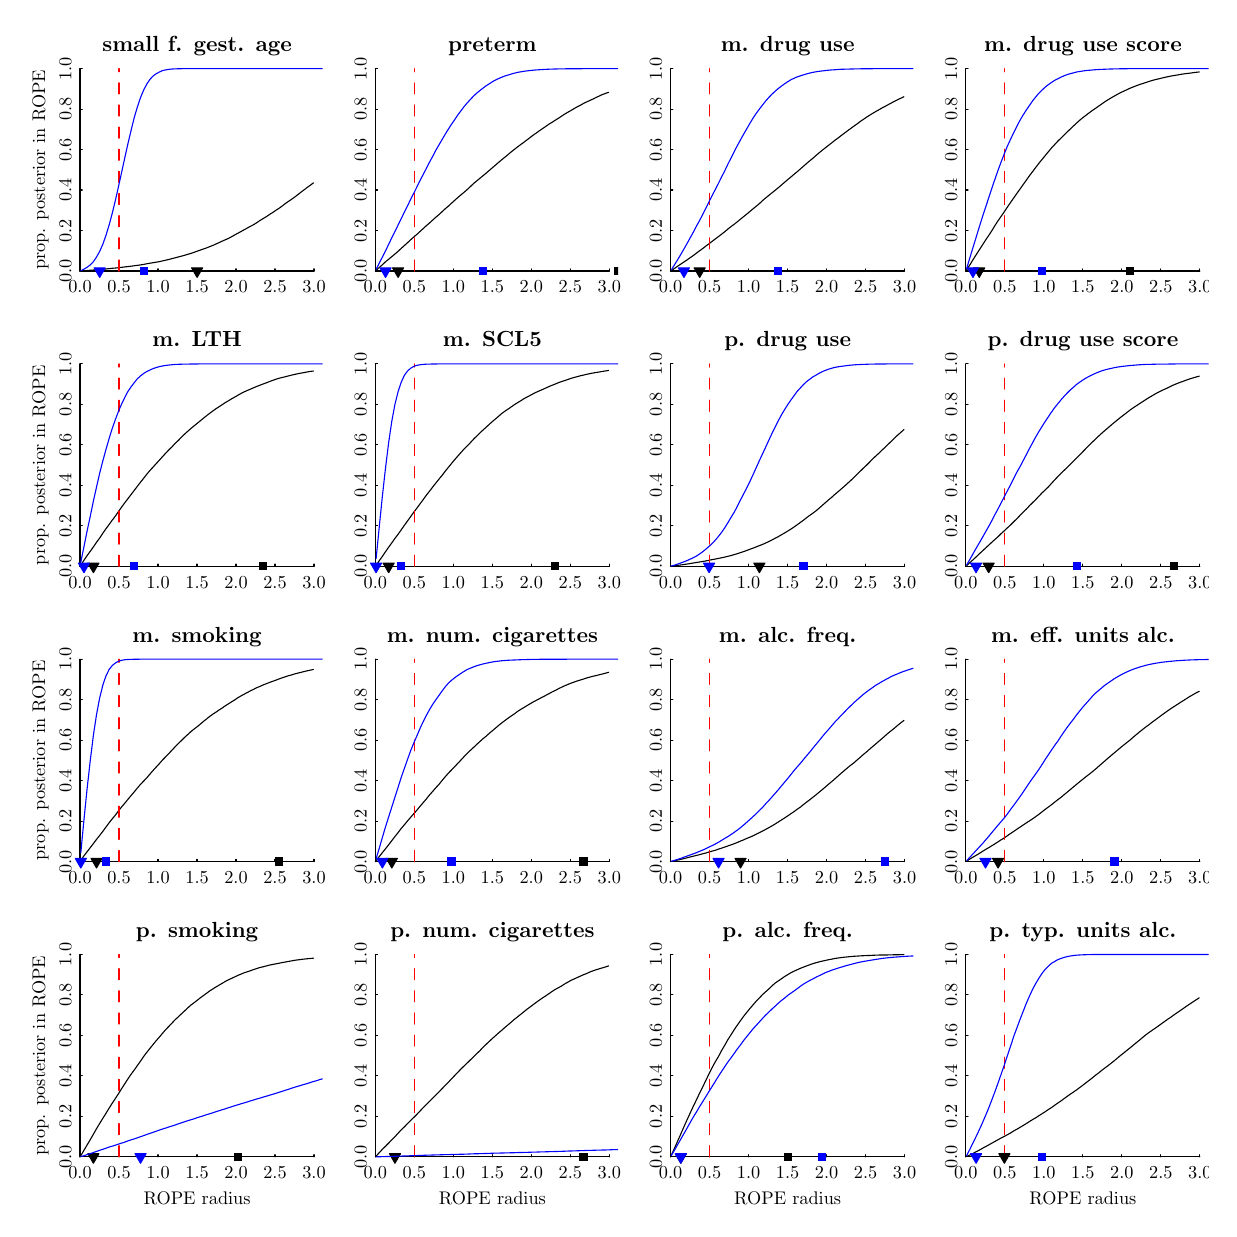
\begin{tikzpicture}[x=1pt,y=1pt]
\definecolor{fillColor}{RGB}{255,255,255}
\path[use as bounding box,fill=fillColor,fill opacity=0.00] (0,0) rectangle (426.79,426.79);
\begin{scope}
\path[clip] ( 15.84,335.93) rectangle (106.62,414.91);
\definecolor{drawColor}{RGB}{0,0,0}

\path[draw=drawColor,line width= 0.4pt,line join=round,line cap=round] ( 19.20,338.87) --
	( 20.34,338.94) --
	( 21.47,339.02) --
	( 22.61,339.13) --
	( 23.75,339.21) --
	( 24.88,339.31) --
	( 26.02,339.40) --
	( 27.15,339.50) --
	( 28.29,339.59) --
	( 29.42,339.72) --
	( 30.56,339.84) --
	( 31.70,339.93) --
	( 32.83,340.05) --
	( 33.97,340.19) --
	( 35.10,340.34) --
	( 36.24,340.46) --
	( 37.38,340.60) --
	( 38.51,340.76) --
	( 39.65,340.90) --
	( 40.78,341.06) --
	( 41.92,341.25) --
	( 43.06,341.48) --
	( 44.19,341.67) --
	( 45.33,341.87) --
	( 46.46,342.05) --
	( 47.60,342.24) --
	( 48.73,342.51) --
	( 49.87,342.77) --
	( 51.01,343.03) --
	( 52.14,343.33) --
	( 53.28,343.63) --
	( 54.41,343.92) --
	( 55.55,344.22) --
	( 56.69,344.54) --
	( 57.82,344.88) --
	( 58.96,345.21) --
	( 60.09,345.59) --
	( 61.23,346.01) --
	( 62.37,346.42) --
	( 63.50,346.81) --
	( 64.64,347.21) --
	( 65.77,347.66) --
	( 66.91,348.11) --
	( 68.04,348.61) --
	( 69.18,349.13) --
	( 70.32,349.66) --
	( 71.45,350.16) --
	( 72.59,350.65) --
	( 73.72,351.27) --
	( 74.86,351.92) --
	( 76.00,352.53) --
	( 77.13,353.14) --
	( 78.27,353.79) --
	( 79.40,354.40) --
	( 80.54,355.04) --
	( 81.67,355.61) --
	( 82.81,356.34) --
	( 83.95,357.11) --
	( 85.08,357.79) --
	( 86.22,358.48) --
	( 87.35,359.25) --
	( 88.49,359.97) --
	( 89.63,360.75) --
	( 90.76,361.46) --
	( 91.90,362.29) --
	( 93.03,363.18) --
	( 94.17,363.98) --
	( 95.31,364.74) --
	( 96.44,365.53) --
	( 97.58,366.41) --
	( 98.71,367.30) --
	( 99.85,368.16) --
	(100.98,369.03) --
	(102.12,369.85) --
	(103.26,370.71);
\end{scope}
\begin{scope}
\path[clip] (  0.00,320.09) rectangle (106.70,426.79);
\definecolor{drawColor}{RGB}{0,0,0}

\node[text=drawColor,rotate= 90.00,anchor=base,inner sep=0pt, outer sep=0pt, scale=  0.66] at (  6.34,375.42) {prop. posterior in ROPE};

\node[text=drawColor,anchor=base,inner sep=0pt, outer sep=0pt, scale=  0.79] at ( 61.23,418.12) {\bfseries small f. gest. age};
\end{scope}
\begin{scope}
\path[clip] (  0.00,  0.00) rectangle (426.79,426.79);
\definecolor{drawColor}{RGB}{0,0,0}

\path[draw=drawColor,line width= 0.4pt,line join=round,line cap=round] ( 18.92,338.86) -- (103.47,338.86);

\path[draw=drawColor,line width= 0.4pt,line join=round,line cap=round] ( 18.92,338.86) -- ( 18.92,339.65);

\path[draw=drawColor,line width= 0.4pt,line join=round,line cap=round] ( 33.01,338.86) -- ( 33.01,339.65);

\path[draw=drawColor,line width= 0.4pt,line join=round,line cap=round] ( 47.10,338.86) -- ( 47.10,339.65);

\path[draw=drawColor,line width= 0.4pt,line join=round,line cap=round] ( 61.20,338.86) -- ( 61.20,339.65);

\path[draw=drawColor,line width= 0.4pt,line join=round,line cap=round] ( 75.29,338.86) -- ( 75.29,339.65);

\path[draw=drawColor,line width= 0.4pt,line join=round,line cap=round] ( 89.38,338.86) -- ( 89.38,339.65);

\path[draw=drawColor,line width= 0.4pt,line join=round,line cap=round] (103.47,338.86) -- (103.47,339.65);

\node[text=drawColor,anchor=base,inner sep=0pt, outer sep=0pt, scale=  0.66] at ( 18.92,330.94) {0.0};

\node[text=drawColor,anchor=base,inner sep=0pt, outer sep=0pt, scale=  0.66] at ( 33.01,330.94) {0.5};

\node[text=drawColor,anchor=base,inner sep=0pt, outer sep=0pt, scale=  0.66] at ( 47.10,330.94) {1.0};

\node[text=drawColor,anchor=base,inner sep=0pt, outer sep=0pt, scale=  0.66] at ( 61.20,330.94) {1.5};

\node[text=drawColor,anchor=base,inner sep=0pt, outer sep=0pt, scale=  0.66] at ( 75.29,330.94) {2.0};

\node[text=drawColor,anchor=base,inner sep=0pt, outer sep=0pt, scale=  0.66] at ( 89.38,330.94) {2.5};

\node[text=drawColor,anchor=base,inner sep=0pt, outer sep=0pt, scale=  0.66] at (103.47,330.94) {3.0};

\path[draw=drawColor,line width= 0.4pt,line join=round,line cap=round] ( 18.92,338.86) -- ( 18.92,411.99);

\path[draw=drawColor,line width= 0.4pt,line join=round,line cap=round] ( 18.92,338.86) -- ( 19.71,338.86);

\path[draw=drawColor,line width= 0.4pt,line join=round,line cap=round] ( 18.92,353.48) -- ( 19.71,353.48);

\path[draw=drawColor,line width= 0.4pt,line join=round,line cap=round] ( 18.92,368.11) -- ( 19.71,368.11);

\path[draw=drawColor,line width= 0.4pt,line join=round,line cap=round] ( 18.92,382.74) -- ( 19.71,382.74);

\path[draw=drawColor,line width= 0.4pt,line join=round,line cap=round] ( 18.92,397.36) -- ( 19.71,397.36);

\path[draw=drawColor,line width= 0.4pt,line join=round,line cap=round] ( 18.92,411.99) -- ( 19.71,411.99);

\node[text=drawColor,rotate= 90.00,anchor=base,inner sep=0pt, outer sep=0pt, scale=  0.66] at ( 15.75,338.86) {0.0};

\node[text=drawColor,rotate= 90.00,anchor=base,inner sep=0pt, outer sep=0pt, scale=  0.66] at ( 15.75,353.48) {0.2};

\node[text=drawColor,rotate= 90.00,anchor=base,inner sep=0pt, outer sep=0pt, scale=  0.66] at ( 15.75,368.11) {0.4};

\node[text=drawColor,rotate= 90.00,anchor=base,inner sep=0pt, outer sep=0pt, scale=  0.66] at ( 15.75,382.74) {0.6};

\node[text=drawColor,rotate= 90.00,anchor=base,inner sep=0pt, outer sep=0pt, scale=  0.66] at ( 15.75,397.36) {0.8};

\node[text=drawColor,rotate= 90.00,anchor=base,inner sep=0pt, outer sep=0pt, scale=  0.66] at ( 15.75,411.99) {1.0};
\end{scope}
\begin{scope}
\path[clip] ( 15.84,335.93) rectangle (106.62,414.91);
\definecolor{drawColor}{RGB}{0,0,0}

\path[draw=drawColor,line width= 0.4pt,line join=round,line cap=round] (131.65,338.86) --
	(131.65,411.99);
\definecolor{drawColor}{RGB}{255,0,0}

\path[draw=drawColor,line width= 0.4pt,dash pattern=on 4pt off 4pt ,line join=round,line cap=round] ( 33.01,338.86) --
	( 33.01,411.99);
\definecolor{fillColor}{RGB}{0,0,0}

\path[fill=fillColor] (130.17,337.37) --
	(133.14,337.37) --
	(133.14,340.34) --
	(130.17,340.34) --
	cycle;
\definecolor{drawColor}{RGB}{0,0,0}

\path[draw=drawColor,line width= 0.4pt,line join=round,line cap=round,fill=fillColor] ( 61.23,336.55) --
	( 63.23,340.01) --
	( 59.23,340.01) --
	cycle;
\definecolor{drawColor}{RGB}{0,0,255}

\path[draw=drawColor,line width= 0.4pt,line join=round,line cap=round] ( 19.20,338.95) --
	( 20.34,339.52) --
	( 21.47,340.21) --
	( 22.61,341.07) --
	( 23.75,342.24) --
	( 24.88,343.90) --
	( 26.02,345.96) --
	( 27.15,348.51) --
	( 28.29,351.73) --
	( 29.42,355.45) --
	( 30.56,359.70) --
	( 31.70,364.40) --
	( 32.83,369.43) --
	( 33.97,374.60) --
	( 35.10,379.80) --
	( 36.24,384.92) --
	( 37.38,389.72) --
	( 38.51,394.31) --
	( 39.65,398.16) --
	( 40.78,401.51) --
	( 41.92,404.26) --
	( 43.06,406.44) --
	( 44.19,408.12) --
	( 45.33,409.33) --
	( 46.46,410.16) --
	( 47.60,410.76) --
	( 48.73,411.28) --
	( 49.87,411.52) --
	( 51.01,411.72) --
	( 52.14,411.84) --
	( 53.28,411.90) --
	( 54.41,411.94) --
	( 55.55,411.96) --
	( 56.69,411.97) --
	( 57.82,411.98) --
	( 58.96,411.99) --
	( 60.09,411.99) --
	( 61.23,411.99) --
	( 62.37,411.99) --
	( 63.50,411.99) --
	( 64.64,411.99) --
	( 65.77,411.99) --
	( 66.91,411.99) --
	( 68.04,411.99) --
	( 69.18,411.99) --
	( 70.32,411.99) --
	( 71.45,411.99) --
	( 72.59,411.99) --
	( 73.72,411.99) --
	( 74.86,411.99) --
	( 76.00,411.99) --
	( 77.13,411.99) --
	( 78.27,411.99) --
	( 79.40,411.99) --
	( 80.54,411.99) --
	( 81.67,411.99) --
	( 82.81,411.99) --
	( 83.95,411.99) --
	( 85.08,411.99) --
	( 86.22,411.99) --
	( 87.35,411.99) --
	( 88.49,411.99) --
	( 89.63,411.99) --
	( 90.76,411.99) --
	( 91.90,411.99) --
	( 93.03,411.99) --
	( 94.17,411.99) --
	( 95.31,411.99) --
	( 96.44,411.99) --
	( 97.58,411.99) --
	( 98.71,411.99) --
	( 99.85,411.99) --
	(100.98,411.99) --
	(102.12,411.99) --
	(103.26,411.99) --
	(104.39,411.99) --
	(105.53,411.99) --
	(106.66,411.99) --
	(107.80,411.99) --
	(108.94,411.99) --
	(110.07,411.99) --
	(111.21,411.99) --
	(112.34,411.99) --
	(113.48,411.99) --
	(114.62,411.99) --
	(115.75,411.99) --
	(116.89,411.99) --
	(118.02,411.99) --
	(119.16,411.99) --
	(120.29,411.99) --
	(121.43,411.99) --
	(122.57,411.99) --
	(123.70,411.99) --
	(124.84,411.99) --
	(125.97,411.99) --
	(127.11,411.99) --
	(128.25,411.99) --
	(129.38,411.99) --
	(130.52,411.99) --
	(131.65,411.99);
\definecolor{fillColor}{RGB}{0,0,255}

\path[fill=fillColor] ( 40.43,337.37) --
	( 43.40,337.37) --
	( 43.40,340.34) --
	( 40.43,340.34) --
	cycle;

\path[draw=drawColor,line width= 0.4pt,line join=round,line cap=round,fill=fillColor] ( 26.02,336.55) --
	( 28.02,340.01) --
	( 24.02,340.01) --
	cycle;
\end{scope}
\begin{scope}
\path[clip] (122.54,335.93) rectangle (213.32,414.91);
\definecolor{drawColor}{RGB}{0,0,0}

\path[draw=drawColor,line width= 0.4pt,line join=round,line cap=round] (125.90,339.10) --
	(127.04,340.10) --
	(128.17,341.11) --
	(129.31,342.20) --
	(130.44,343.10) --
	(131.58,344.06) --
	(132.72,345.01) --
	(133.85,345.97) --
	(134.99,347.04) --
	(136.12,348.06) --
	(137.26,349.08) --
	(138.39,350.15) --
	(139.53,351.16) --
	(140.67,352.12) --
	(141.80,353.16) --
	(142.94,354.20) --
	(144.07,355.24) --
	(145.21,356.22) --
	(146.35,357.26) --
	(147.48,358.29) --
	(148.62,359.24) --
	(149.75,360.29) --
	(150.89,361.35) --
	(152.02,362.30) --
	(153.16,363.37) --
	(154.30,364.39) --
	(155.43,365.40) --
	(156.57,366.38) --
	(157.70,367.30) --
	(158.84,368.30) --
	(159.98,369.37) --
	(161.11,370.46) --
	(162.25,371.40) --
	(163.38,372.34) --
	(164.52,373.27) --
	(165.66,374.22) --
	(166.79,375.19) --
	(167.93,376.19) --
	(169.06,377.13) --
	(170.20,378.14) --
	(171.33,379.08) --
	(172.47,380.01) --
	(173.61,380.95) --
	(174.74,381.92) --
	(175.88,382.81) --
	(177.01,383.70) --
	(178.15,384.54) --
	(179.29,385.37) --
	(180.42,386.22) --
	(181.56,387.11) --
	(182.69,387.96) --
	(183.83,388.76) --
	(184.97,389.57) --
	(186.10,390.36) --
	(187.24,391.13) --
	(188.37,391.92) --
	(189.51,392.61) --
	(190.64,393.34) --
	(191.78,394.06) --
	(192.92,394.80) --
	(194.05,395.55) --
	(195.19,396.23) --
	(196.32,396.86) --
	(197.46,397.54) --
	(198.60,398.20) --
	(199.73,398.77) --
	(200.87,399.42) --
	(202.00,399.96) --
	(203.14,400.47) --
	(204.27,401.00) --
	(205.41,401.58) --
	(206.55,402.09) --
	(207.68,402.62) --
	(208.82,403.04) --
	(209.95,403.44);
\end{scope}
\begin{scope}
\path[clip] (106.70,320.09) rectangle (213.40,426.79);
\definecolor{drawColor}{RGB}{0,0,0}

\node[text=drawColor,anchor=base,inner sep=0pt, outer sep=0pt, scale=  0.79] at (167.93,418.12) {\bfseries preterm};
\end{scope}
\begin{scope}
\path[clip] (  0.00,  0.00) rectangle (426.79,426.79);
\definecolor{drawColor}{RGB}{0,0,0}

\path[draw=drawColor,line width= 0.4pt,line join=round,line cap=round] (125.62,338.86) -- (210.17,338.86);

\path[draw=drawColor,line width= 0.4pt,line join=round,line cap=round] (125.62,338.86) -- (125.62,339.65);

\path[draw=drawColor,line width= 0.4pt,line join=round,line cap=round] (139.71,338.86) -- (139.71,339.65);

\path[draw=drawColor,line width= 0.4pt,line join=round,line cap=round] (153.80,338.86) -- (153.80,339.65);

\path[draw=drawColor,line width= 0.4pt,line join=round,line cap=round] (167.89,338.86) -- (167.89,339.65);

\path[draw=drawColor,line width= 0.4pt,line join=round,line cap=round] (181.98,338.86) -- (181.98,339.65);

\path[draw=drawColor,line width= 0.4pt,line join=round,line cap=round] (196.08,338.86) -- (196.08,339.65);

\path[draw=drawColor,line width= 0.4pt,line join=round,line cap=round] (210.17,338.86) -- (210.17,339.65);

\node[text=drawColor,anchor=base,inner sep=0pt, outer sep=0pt, scale=  0.66] at (125.62,330.94) {0.0};

\node[text=drawColor,anchor=base,inner sep=0pt, outer sep=0pt, scale=  0.66] at (139.71,330.94) {0.5};

\node[text=drawColor,anchor=base,inner sep=0pt, outer sep=0pt, scale=  0.66] at (153.80,330.94) {1.0};

\node[text=drawColor,anchor=base,inner sep=0pt, outer sep=0pt, scale=  0.66] at (167.89,330.94) {1.5};

\node[text=drawColor,anchor=base,inner sep=0pt, outer sep=0pt, scale=  0.66] at (181.98,330.94) {2.0};

\node[text=drawColor,anchor=base,inner sep=0pt, outer sep=0pt, scale=  0.66] at (196.08,330.94) {2.5};

\node[text=drawColor,anchor=base,inner sep=0pt, outer sep=0pt, scale=  0.66] at (210.17,330.94) {3.0};

\path[draw=drawColor,line width= 0.4pt,line join=round,line cap=round] (125.62,338.86) -- (125.62,411.99);

\path[draw=drawColor,line width= 0.4pt,line join=round,line cap=round] (125.62,338.86) -- (126.41,338.86);

\path[draw=drawColor,line width= 0.4pt,line join=round,line cap=round] (125.62,353.48) -- (126.41,353.48);

\path[draw=drawColor,line width= 0.4pt,line join=round,line cap=round] (125.62,368.11) -- (126.41,368.11);

\path[draw=drawColor,line width= 0.4pt,line join=round,line cap=round] (125.62,382.74) -- (126.41,382.74);

\path[draw=drawColor,line width= 0.4pt,line join=round,line cap=round] (125.62,397.36) -- (126.41,397.36);

\path[draw=drawColor,line width= 0.4pt,line join=round,line cap=round] (125.62,411.99) -- (126.41,411.99);

\node[text=drawColor,rotate= 90.00,anchor=base,inner sep=0pt, outer sep=0pt, scale=  0.66] at (122.45,338.86) {0.0};

\node[text=drawColor,rotate= 90.00,anchor=base,inner sep=0pt, outer sep=0pt, scale=  0.66] at (122.45,353.48) {0.2};

\node[text=drawColor,rotate= 90.00,anchor=base,inner sep=0pt, outer sep=0pt, scale=  0.66] at (122.45,368.11) {0.4};

\node[text=drawColor,rotate= 90.00,anchor=base,inner sep=0pt, outer sep=0pt, scale=  0.66] at (122.45,382.74) {0.6};

\node[text=drawColor,rotate= 90.00,anchor=base,inner sep=0pt, outer sep=0pt, scale=  0.66] at (122.45,397.36) {0.8};

\node[text=drawColor,rotate= 90.00,anchor=base,inner sep=0pt, outer sep=0pt, scale=  0.66] at (122.45,411.99) {1.0};
\end{scope}
\begin{scope}
\path[clip] (122.54,335.93) rectangle (213.32,414.91);
\definecolor{drawColor}{RGB}{0,0,0}

\path[draw=drawColor,line width= 0.4pt,line join=round,line cap=round] (238.35,338.86) --
	(238.35,411.99);
\definecolor{drawColor}{RGB}{255,0,0}

\path[draw=drawColor,line width= 0.4pt,dash pattern=on 4pt off 4pt ,line join=round,line cap=round] (139.71,338.86) --
	(139.71,411.99);
\definecolor{fillColor}{RGB}{0,0,0}

\path[fill=fillColor] (211.88,337.37) --
	(214.85,337.37) --
	(214.85,340.34) --
	(211.88,340.34) --
	cycle;
\definecolor{drawColor}{RGB}{0,0,0}

\path[draw=drawColor,line width= 0.4pt,line join=round,line cap=round,fill=fillColor] (133.85,336.55) --
	(135.85,340.01) --
	(131.85,340.01) --
	cycle;
\definecolor{drawColor}{RGB}{0,0,255}

\path[draw=drawColor,line width= 0.4pt,line join=round,line cap=round] (125.90,339.47) --
	(127.04,341.72) --
	(128.17,343.91) --
	(129.31,346.13) --
	(130.44,348.51) --
	(131.58,350.86) --
	(132.72,353.14) --
	(133.85,355.47) --
	(134.99,357.81) --
	(136.12,360.12) --
	(137.26,362.41) --
	(138.39,364.78) --
	(139.53,366.99) --
	(140.67,369.29) --
	(141.80,371.59) --
	(142.94,373.79) --
	(144.07,375.96) --
	(145.21,378.19) --
	(146.35,380.29) --
	(147.48,382.47) --
	(148.62,384.43) --
	(149.75,386.36) --
	(150.89,388.31) --
	(152.02,390.13) --
	(153.16,391.91) --
	(154.30,393.55) --
	(155.43,395.25) --
	(156.57,396.76) --
	(157.70,398.27) --
	(158.84,399.61) --
	(159.98,400.85) --
	(161.11,402.06) --
	(162.25,403.12) --
	(163.38,404.04) --
	(164.52,404.92) --
	(165.66,405.80) --
	(166.79,406.49) --
	(167.93,407.25) --
	(169.06,407.88) --
	(170.20,408.42) --
	(171.33,408.90) --
	(172.47,409.33) --
	(173.61,409.67) --
	(174.74,410.04) --
	(175.88,410.35) --
	(177.01,410.63) --
	(178.15,410.83) --
	(179.29,411.02) --
	(180.42,411.17) --
	(181.56,411.30) --
	(182.69,411.42) --
	(183.83,411.52) --
	(184.97,411.60) --
	(186.10,411.66) --
	(187.24,411.73) --
	(188.37,411.78) --
	(189.51,411.82) --
	(190.64,411.85) --
	(191.78,411.88) --
	(192.92,411.89) --
	(194.05,411.92) --
	(195.19,411.93) --
	(196.32,411.93) --
	(197.46,411.94) --
	(198.60,411.95) --
	(199.73,411.95) --
	(200.87,411.97) --
	(202.00,411.97) --
	(203.14,411.98) --
	(204.27,411.98) --
	(205.41,411.98) --
	(206.55,411.98) --
	(207.68,411.98) --
	(208.82,411.98) --
	(209.95,411.98) --
	(211.09,411.98) --
	(212.23,411.98) --
	(213.36,411.98) --
	(214.50,411.98) --
	(215.63,411.98) --
	(216.77,411.98) --
	(217.91,411.99) --
	(219.04,411.99) --
	(220.18,411.99) --
	(221.31,411.99) --
	(222.45,411.99) --
	(223.58,411.99) --
	(224.72,411.99) --
	(225.86,411.99) --
	(226.99,411.99) --
	(228.13,411.99) --
	(229.26,411.99) --
	(230.40,411.99) --
	(231.54,411.99) --
	(232.67,411.99) --
	(233.81,411.99) --
	(234.94,411.99) --
	(236.08,411.99) --
	(237.22,411.99) --
	(238.35,411.99);
\definecolor{fillColor}{RGB}{0,0,255}

\path[fill=fillColor] (163.03,337.37) --
	(166.00,337.37) --
	(166.00,340.34) --
	(163.03,340.34) --
	cycle;

\path[draw=drawColor,line width= 0.4pt,line join=round,line cap=round,fill=fillColor] (129.31,336.55) --
	(131.31,340.01) --
	(127.31,340.01) --
	cycle;
\end{scope}
\begin{scope}
\path[clip] (229.24,335.93) rectangle (320.01,414.91);
\definecolor{drawColor}{RGB}{0,0,0}

\path[draw=drawColor,line width= 0.4pt,line join=round,line cap=round] (232.60,339.00) --
	(233.73,339.79) --
	(234.87,340.60) --
	(236.01,341.36) --
	(237.14,342.11) --
	(238.28,342.88) --
	(239.41,343.68) --
	(240.55,344.47) --
	(241.68,345.33) --
	(242.82,346.20) --
	(243.96,346.99) --
	(245.09,347.89) --
	(246.23,348.72) --
	(247.36,349.60) --
	(248.50,350.46) --
	(249.64,351.32) --
	(250.77,352.18) --
	(251.91,353.06) --
	(253.04,354.04) --
	(254.18,354.93) --
	(255.32,355.77) --
	(256.45,356.66) --
	(257.59,357.61) --
	(258.72,358.52) --
	(259.86,359.44) --
	(260.99,360.39) --
	(262.13,361.34) --
	(263.27,362.27) --
	(264.40,363.21) --
	(265.54,364.30) --
	(266.67,365.26) --
	(267.81,366.18) --
	(268.95,367.10) --
	(270.08,368.01) --
	(271.22,368.94) --
	(272.35,369.90) --
	(273.49,370.89) --
	(274.62,371.87) --
	(275.76,372.79) --
	(276.90,373.79) --
	(278.03,374.71) --
	(279.17,375.69) --
	(280.30,376.69) --
	(281.44,377.69) --
	(282.58,378.66) --
	(283.71,379.57) --
	(284.85,380.59) --
	(285.98,381.55) --
	(287.12,382.50) --
	(288.26,383.39) --
	(289.39,384.28) --
	(290.53,385.16) --
	(291.66,386.07) --
	(292.80,386.90) --
	(293.93,387.77) --
	(295.07,388.63) --
	(296.21,389.49) --
	(297.34,390.31) --
	(298.48,391.15) --
	(299.61,391.95) --
	(300.75,392.81) --
	(301.89,393.59) --
	(303.02,394.37) --
	(304.16,395.10) --
	(305.29,395.80) --
	(306.43,396.48) --
	(307.57,397.10) --
	(308.70,397.76) --
	(309.84,398.35) --
	(310.97,398.98) --
	(312.11,399.59) --
	(313.24,400.18) --
	(314.38,400.78) --
	(315.52,401.30) --
	(316.65,401.85);
\end{scope}
\begin{scope}
\path[clip] (213.40,320.09) rectangle (320.09,426.79);
\definecolor{drawColor}{RGB}{0,0,0}

\node[text=drawColor,anchor=base,inner sep=0pt, outer sep=0pt, scale=  0.79] at (274.62,418.12) {\bfseries m. drug use};
\end{scope}
\begin{scope}
\path[clip] (  0.00,  0.00) rectangle (426.79,426.79);
\definecolor{drawColor}{RGB}{0,0,0}

\path[draw=drawColor,line width= 0.4pt,line join=round,line cap=round] (232.32,338.86) -- (316.87,338.86);

\path[draw=drawColor,line width= 0.4pt,line join=round,line cap=round] (232.32,338.86) -- (232.32,339.65);

\path[draw=drawColor,line width= 0.4pt,line join=round,line cap=round] (246.41,338.86) -- (246.41,339.65);

\path[draw=drawColor,line width= 0.4pt,line join=round,line cap=round] (260.50,338.86) -- (260.50,339.65);

\path[draw=drawColor,line width= 0.4pt,line join=round,line cap=round] (274.59,338.86) -- (274.59,339.65);

\path[draw=drawColor,line width= 0.4pt,line join=round,line cap=round] (288.68,338.86) -- (288.68,339.65);

\path[draw=drawColor,line width= 0.4pt,line join=round,line cap=round] (302.77,338.86) -- (302.77,339.65);

\path[draw=drawColor,line width= 0.4pt,line join=round,line cap=round] (316.87,338.86) -- (316.87,339.65);

\node[text=drawColor,anchor=base,inner sep=0pt, outer sep=0pt, scale=  0.66] at (232.32,330.94) {0.0};

\node[text=drawColor,anchor=base,inner sep=0pt, outer sep=0pt, scale=  0.66] at (246.41,330.94) {0.5};

\node[text=drawColor,anchor=base,inner sep=0pt, outer sep=0pt, scale=  0.66] at (260.50,330.94) {1.0};

\node[text=drawColor,anchor=base,inner sep=0pt, outer sep=0pt, scale=  0.66] at (274.59,330.94) {1.5};

\node[text=drawColor,anchor=base,inner sep=0pt, outer sep=0pt, scale=  0.66] at (288.68,330.94) {2.0};

\node[text=drawColor,anchor=base,inner sep=0pt, outer sep=0pt, scale=  0.66] at (302.77,330.94) {2.5};

\node[text=drawColor,anchor=base,inner sep=0pt, outer sep=0pt, scale=  0.66] at (316.87,330.94) {3.0};

\path[draw=drawColor,line width= 0.4pt,line join=round,line cap=round] (232.32,338.86) -- (232.32,411.99);

\path[draw=drawColor,line width= 0.4pt,line join=round,line cap=round] (232.32,338.86) -- (233.11,338.86);

\path[draw=drawColor,line width= 0.4pt,line join=round,line cap=round] (232.32,353.48) -- (233.11,353.48);

\path[draw=drawColor,line width= 0.4pt,line join=round,line cap=round] (232.32,368.11) -- (233.11,368.11);

\path[draw=drawColor,line width= 0.4pt,line join=round,line cap=round] (232.32,382.74) -- (233.11,382.74);

\path[draw=drawColor,line width= 0.4pt,line join=round,line cap=round] (232.32,397.36) -- (233.11,397.36);

\path[draw=drawColor,line width= 0.4pt,line join=round,line cap=round] (232.32,411.99) -- (233.11,411.99);

\node[text=drawColor,rotate= 90.00,anchor=base,inner sep=0pt, outer sep=0pt, scale=  0.66] at (229.15,338.86) {0.0};

\node[text=drawColor,rotate= 90.00,anchor=base,inner sep=0pt, outer sep=0pt, scale=  0.66] at (229.15,353.48) {0.2};

\node[text=drawColor,rotate= 90.00,anchor=base,inner sep=0pt, outer sep=0pt, scale=  0.66] at (229.15,368.11) {0.4};

\node[text=drawColor,rotate= 90.00,anchor=base,inner sep=0pt, outer sep=0pt, scale=  0.66] at (229.15,382.74) {0.6};

\node[text=drawColor,rotate= 90.00,anchor=base,inner sep=0pt, outer sep=0pt, scale=  0.66] at (229.15,397.36) {0.8};

\node[text=drawColor,rotate= 90.00,anchor=base,inner sep=0pt, outer sep=0pt, scale=  0.66] at (229.15,411.99) {1.0};
\end{scope}
\begin{scope}
\path[clip] (229.24,335.93) rectangle (320.01,414.91);
\definecolor{drawColor}{RGB}{0,0,0}

\path[draw=drawColor,line width= 0.4pt,line join=round,line cap=round] (345.05,338.86) --
	(345.05,411.99);
\definecolor{drawColor}{RGB}{255,0,0}

\path[draw=drawColor,line width= 0.4pt,dash pattern=on 4pt off 4pt ,line join=round,line cap=round] (246.41,338.86) --
	(246.41,411.99);
\definecolor{fillColor}{RGB}{0,0,0}

\path[fill=fillColor] (321.98,337.37) --
	(324.95,337.37) --
	(324.95,340.34) --
	(321.98,340.34) --
	cycle;
\definecolor{drawColor}{RGB}{0,0,0}

\path[draw=drawColor,line width= 0.4pt,line join=round,line cap=round,fill=fillColor] (242.82,336.55) --
	(244.82,340.01) --
	(240.82,340.01) --
	cycle;
\definecolor{drawColor}{RGB}{0,0,255}

\path[draw=drawColor,line width= 0.4pt,line join=round,line cap=round] (232.60,339.26) --
	(233.73,341.11) --
	(234.87,342.93) --
	(236.01,344.85) --
	(237.14,346.82) --
	(238.28,348.83) --
	(239.41,350.87) --
	(240.55,352.94) --
	(241.68,355.11) --
	(242.82,357.16) --
	(243.96,359.39) --
	(245.09,361.63) --
	(246.23,363.96) --
	(247.36,366.19) --
	(248.50,368.35) --
	(249.64,370.59) --
	(250.77,372.87) --
	(251.91,375.12) --
	(253.04,377.49) --
	(254.18,379.75) --
	(255.32,382.03) --
	(256.45,384.19) --
	(257.59,386.27) --
	(258.72,388.33) --
	(259.86,390.28) --
	(260.99,392.25) --
	(262.13,394.14) --
	(263.27,395.83) --
	(264.40,397.36) --
	(265.54,398.85) --
	(266.67,400.28) --
	(267.81,401.57) --
	(268.95,402.74) --
	(270.08,403.82) --
	(271.22,404.80) --
	(272.35,405.66) --
	(273.49,406.50) --
	(274.62,407.23) --
	(275.76,407.95) --
	(276.90,408.49) --
	(278.03,409.00) --
	(279.17,409.38) --
	(280.30,409.73) --
	(281.44,410.07) --
	(282.58,410.38) --
	(283.71,410.64) --
	(284.85,410.84) --
	(285.98,411.02) --
	(287.12,411.15) --
	(288.26,411.29) --
	(289.39,411.42) --
	(290.53,411.52) --
	(291.66,411.58) --
	(292.80,411.68) --
	(293.93,411.75) --
	(295.07,411.78) --
	(296.21,411.81) --
	(297.34,411.84) --
	(298.48,411.87) --
	(299.61,411.90) --
	(300.75,411.92) --
	(301.89,411.93) --
	(303.02,411.94) --
	(304.16,411.95) --
	(305.29,411.96) --
	(306.43,411.97) --
	(307.57,411.97) --
	(308.70,411.98) --
	(309.84,411.98) --
	(310.97,411.98) --
	(312.11,411.98) --
	(313.24,411.98) --
	(314.38,411.98) --
	(315.52,411.98) --
	(316.65,411.98) --
	(317.79,411.98) --
	(318.92,411.98) --
	(320.06,411.99) --
	(321.20,411.99) --
	(322.33,411.99) --
	(323.47,411.99) --
	(324.60,411.99) --
	(325.74,411.99) --
	(326.87,411.99) --
	(328.01,411.99) --
	(329.15,411.99) --
	(330.28,411.99) --
	(331.42,411.99) --
	(332.55,411.99) --
	(333.69,411.99) --
	(334.83,411.99) --
	(335.96,411.99) --
	(337.10,411.99) --
	(338.23,411.99) --
	(339.37,411.99) --
	(340.51,411.99) --
	(341.64,411.99) --
	(342.78,411.99) --
	(343.91,411.99) --
	(345.05,411.99);
\definecolor{fillColor}{RGB}{0,0,255}

\path[fill=fillColor] (269.73,337.37) --
	(272.70,337.37) --
	(272.70,340.34) --
	(269.73,340.34) --
	cycle;

\path[draw=drawColor,line width= 0.4pt,line join=round,line cap=round,fill=fillColor] (237.14,336.55) --
	(239.14,340.01) --
	(235.14,340.01) --
	cycle;
\end{scope}
\begin{scope}
\path[clip] (335.93,335.93) rectangle (426.71,414.91);
\definecolor{drawColor}{RGB}{0,0,0}

\path[draw=drawColor,line width= 0.4pt,line join=round,line cap=round] (339.30,339.28) --
	(340.43,341.02) --
	(341.57,342.91) --
	(342.70,344.68) --
	(343.84,346.46) --
	(344.98,348.22) --
	(346.11,349.99) --
	(347.25,351.68) --
	(348.38,353.39) --
	(349.52,355.29) --
	(350.65,357.03) --
	(351.79,358.66) --
	(352.93,360.30) --
	(354.06,362.00) --
	(355.20,363.70) --
	(356.33,365.28) --
	(357.47,366.94) --
	(358.61,368.51) --
	(359.74,370.12) --
	(360.88,371.72) --
	(362.01,373.32) --
	(363.15,374.80) --
	(364.28,376.32) --
	(365.42,377.80) --
	(366.56,379.20) --
	(367.69,380.58) --
	(368.83,381.96) --
	(369.96,383.32) --
	(371.10,384.54) --
	(372.24,385.78) --
	(373.37,386.87) --
	(374.51,388.02) --
	(375.64,389.11) --
	(376.78,390.20) --
	(377.92,391.29) --
	(379.05,392.33) --
	(380.19,393.37) --
	(381.32,394.30) --
	(382.46,395.16) --
	(383.59,396.03) --
	(384.73,396.88) --
	(385.87,397.63) --
	(387.00,398.44) --
	(388.14,399.23) --
	(389.27,400.04) --
	(390.41,400.75) --
	(391.55,401.45) --
	(392.68,402.08) --
	(393.82,402.72) --
	(394.95,403.34) --
	(396.09,403.84) --
	(397.22,404.38) --
	(398.36,404.91) --
	(399.50,405.38) --
	(400.63,405.81) --
	(401.77,406.23) --
	(402.90,406.60) --
	(404.04,406.98) --
	(405.18,407.35) --
	(406.31,407.70) --
	(407.45,408.00) --
	(408.58,408.27) --
	(409.72,408.55) --
	(410.86,408.82) --
	(411.99,409.06) --
	(413.13,409.31) --
	(414.26,409.50) --
	(415.40,409.68) --
	(416.53,409.90) --
	(417.67,410.06) --
	(418.81,410.22) --
	(419.94,410.34) --
	(421.08,410.51) --
	(422.21,410.66) --
	(423.35,410.78);
\end{scope}
\begin{scope}
\path[clip] (320.09,320.09) rectangle (426.79,426.79);
\definecolor{drawColor}{RGB}{0,0,0}

\node[text=drawColor,anchor=base,inner sep=0pt, outer sep=0pt, scale=  0.79] at (381.32,418.12) {\bfseries m. drug use score};
\end{scope}
\begin{scope}
\path[clip] (  0.00,  0.00) rectangle (426.79,426.79);
\definecolor{drawColor}{RGB}{0,0,0}

\path[draw=drawColor,line width= 0.4pt,line join=round,line cap=round] (339.01,338.86) -- (423.56,338.86);

\path[draw=drawColor,line width= 0.4pt,line join=round,line cap=round] (339.01,338.86) -- (339.01,339.65);

\path[draw=drawColor,line width= 0.4pt,line join=round,line cap=round] (353.11,338.86) -- (353.11,339.65);

\path[draw=drawColor,line width= 0.4pt,line join=round,line cap=round] (367.20,338.86) -- (367.20,339.65);

\path[draw=drawColor,line width= 0.4pt,line join=round,line cap=round] (381.29,338.86) -- (381.29,339.65);

\path[draw=drawColor,line width= 0.4pt,line join=round,line cap=round] (395.38,338.86) -- (395.38,339.65);

\path[draw=drawColor,line width= 0.4pt,line join=round,line cap=round] (409.47,338.86) -- (409.47,339.65);

\path[draw=drawColor,line width= 0.4pt,line join=round,line cap=round] (423.56,338.86) -- (423.56,339.65);

\node[text=drawColor,anchor=base,inner sep=0pt, outer sep=0pt, scale=  0.66] at (339.01,330.94) {0.0};

\node[text=drawColor,anchor=base,inner sep=0pt, outer sep=0pt, scale=  0.66] at (353.11,330.94) {0.5};

\node[text=drawColor,anchor=base,inner sep=0pt, outer sep=0pt, scale=  0.66] at (367.20,330.94) {1.0};

\node[text=drawColor,anchor=base,inner sep=0pt, outer sep=0pt, scale=  0.66] at (381.29,330.94) {1.5};

\node[text=drawColor,anchor=base,inner sep=0pt, outer sep=0pt, scale=  0.66] at (395.38,330.94) {2.0};

\node[text=drawColor,anchor=base,inner sep=0pt, outer sep=0pt, scale=  0.66] at (409.47,330.94) {2.5};

\node[text=drawColor,anchor=base,inner sep=0pt, outer sep=0pt, scale=  0.66] at (423.56,330.94) {3.0};

\path[draw=drawColor,line width= 0.4pt,line join=round,line cap=round] (339.01,338.86) -- (339.01,411.99);

\path[draw=drawColor,line width= 0.4pt,line join=round,line cap=round] (339.01,338.86) -- (339.80,338.86);

\path[draw=drawColor,line width= 0.4pt,line join=round,line cap=round] (339.01,353.48) -- (339.80,353.48);

\path[draw=drawColor,line width= 0.4pt,line join=round,line cap=round] (339.01,368.11) -- (339.80,368.11);

\path[draw=drawColor,line width= 0.4pt,line join=round,line cap=round] (339.01,382.74) -- (339.80,382.74);

\path[draw=drawColor,line width= 0.4pt,line join=round,line cap=round] (339.01,397.36) -- (339.80,397.36);

\path[draw=drawColor,line width= 0.4pt,line join=round,line cap=round] (339.01,411.99) -- (339.80,411.99);

\node[text=drawColor,rotate= 90.00,anchor=base,inner sep=0pt, outer sep=0pt, scale=  0.66] at (335.85,338.86) {0.0};

\node[text=drawColor,rotate= 90.00,anchor=base,inner sep=0pt, outer sep=0pt, scale=  0.66] at (335.85,353.48) {0.2};

\node[text=drawColor,rotate= 90.00,anchor=base,inner sep=0pt, outer sep=0pt, scale=  0.66] at (335.85,368.11) {0.4};

\node[text=drawColor,rotate= 90.00,anchor=base,inner sep=0pt, outer sep=0pt, scale=  0.66] at (335.85,382.74) {0.6};

\node[text=drawColor,rotate= 90.00,anchor=base,inner sep=0pt, outer sep=0pt, scale=  0.66] at (335.85,397.36) {0.8};

\node[text=drawColor,rotate= 90.00,anchor=base,inner sep=0pt, outer sep=0pt, scale=  0.66] at (335.85,411.99) {1.0};
\end{scope}
\begin{scope}
\path[clip] (335.93,335.93) rectangle (426.71,414.91);
\definecolor{drawColor}{RGB}{255,0,0}

\path[draw=drawColor,line width= 0.4pt,dash pattern=on 4pt off 4pt ,line join=round,line cap=round] (353.11,338.86) --
	(353.11,411.99);
\definecolor{fillColor}{RGB}{0,0,0}

\path[fill=fillColor] (396.88,337.37) --
	(399.85,337.37) --
	(399.85,340.34) --
	(396.88,340.34) --
	cycle;
\definecolor{drawColor}{RGB}{0,0,0}

\path[draw=drawColor,line width= 0.4pt,line join=round,line cap=round,fill=fillColor] (343.84,336.55) --
	(345.84,340.01) --
	(341.84,340.01) --
	cycle;
\definecolor{drawColor}{RGB}{0,0,255}

\path[draw=drawColor,line width= 0.4pt,line join=round,line cap=round] (339.30,339.75) --
	(340.43,343.55) --
	(341.57,347.30) --
	(342.70,350.97) --
	(343.84,354.69) --
	(344.98,358.34) --
	(346.11,361.78) --
	(347.25,365.27) --
	(348.38,368.66) --
	(349.52,372.04) --
	(350.65,375.28) --
	(351.79,378.37) --
	(352.93,381.28) --
	(354.06,384.09) --
	(355.20,386.53) --
	(356.33,388.92) --
	(357.47,391.17) --
	(358.61,393.39) --
	(359.74,395.28) --
	(360.88,397.07) --
	(362.01,398.72) --
	(363.15,400.36) --
	(364.28,401.78) --
	(365.42,403.13) --
	(366.56,404.24) --
	(367.69,405.31) --
	(368.83,406.21) --
	(369.96,407.00) --
	(371.10,407.75) --
	(372.24,408.32) --
	(373.37,408.91) --
	(374.51,409.40) --
	(375.64,409.84) --
	(376.78,410.17) --
	(377.92,410.46) --
	(379.05,410.77) --
	(380.19,410.96) --
	(381.32,411.14) --
	(382.46,411.31) --
	(383.59,411.39) --
	(384.73,411.50) --
	(385.87,411.60) --
	(387.00,411.67) --
	(388.14,411.72) --
	(389.27,411.77) --
	(390.41,411.82) --
	(391.55,411.86) --
	(392.68,411.88) --
	(393.82,411.91) --
	(394.95,411.93) --
	(396.09,411.94) --
	(397.22,411.96) --
	(398.36,411.97) --
	(399.50,411.97) --
	(400.63,411.98) --
	(401.77,411.98) --
	(402.90,411.98) --
	(404.04,411.98) --
	(405.18,411.98) --
	(406.31,411.98) --
	(407.45,411.98) --
	(408.58,411.98) --
	(409.72,411.98) --
	(410.86,411.99) --
	(411.99,411.99) --
	(413.13,411.99) --
	(414.26,411.99) --
	(415.40,411.99) --
	(416.53,411.99) --
	(417.67,411.99) --
	(418.81,411.99) --
	(419.94,411.99) --
	(421.08,411.99) --
	(422.21,411.99) --
	(423.35,411.99) --
	(424.49,411.99) --
	(425.62,411.99) --
	(426.76,411.99) --
	(426.79,411.99);
\definecolor{fillColor}{RGB}{0,0,255}

\path[fill=fillColor] (365.07,337.37) --
	(368.04,337.37) --
	(368.04,340.34) --
	(365.07,340.34) --
	cycle;

\path[draw=drawColor,line width= 0.4pt,line join=round,line cap=round,fill=fillColor] (341.57,336.55) --
	(343.57,340.01) --
	(339.57,340.01) --
	cycle;
\end{scope}
\begin{scope}
\path[clip] ( 15.84,229.24) rectangle (106.62,308.21);
\definecolor{drawColor}{RGB}{0,0,0}

\path[draw=drawColor,line width= 0.4pt,line join=round,line cap=round] ( 19.20,232.57) --
	( 20.34,234.34) --
	( 21.47,236.01) --
	( 22.61,237.57) --
	( 23.75,239.17) --
	( 24.88,240.83) --
	( 26.02,242.37) --
	( 27.15,244.09) --
	( 28.29,245.72) --
	( 29.42,247.24) --
	( 30.56,248.83) --
	( 31.70,250.32) --
	( 32.83,251.97) --
	( 33.97,253.58) --
	( 35.10,255.13) --
	( 36.24,256.61) --
	( 37.38,258.12) --
	( 38.51,259.58) --
	( 39.65,261.08) --
	( 40.78,262.56) --
	( 41.92,263.98) --
	( 43.06,265.45) --
	( 44.19,266.80) --
	( 45.33,268.02) --
	( 46.46,269.27) --
	( 47.60,270.51) --
	( 48.73,271.78) --
	( 49.87,273.02) --
	( 51.01,274.22) --
	( 52.14,275.32) --
	( 53.28,276.57) --
	( 54.41,277.60) --
	( 55.55,278.80) --
	( 56.69,279.90) --
	( 57.82,280.92) --
	( 58.96,281.93) --
	( 60.09,282.86) --
	( 61.23,283.78) --
	( 62.37,284.73) --
	( 63.50,285.65) --
	( 64.64,286.57) --
	( 65.77,287.43) --
	( 66.91,288.28) --
	( 68.04,289.09) --
	( 69.18,289.81) --
	( 70.32,290.58) --
	( 71.45,291.33) --
	( 72.59,291.99) --
	( 73.72,292.69) --
	( 74.86,293.31) --
	( 76.00,293.99) --
	( 77.13,294.63) --
	( 78.27,295.20) --
	( 79.40,295.71) --
	( 80.54,296.18) --
	( 81.67,296.69) --
	( 82.81,297.16) --
	( 83.95,297.60) --
	( 85.08,298.03) --
	( 86.22,298.45) --
	( 87.35,298.90) --
	( 88.49,299.32) --
	( 89.63,299.72) --
	( 90.76,300.07) --
	( 91.90,300.37) --
	( 93.03,300.63) --
	( 94.17,300.94) --
	( 95.31,301.22) --
	( 96.44,301.48) --
	( 97.58,301.73) --
	( 98.71,301.95) --
	( 99.85,302.15) --
	(100.98,302.37) --
	(102.12,302.56) --
	(103.26,302.72);
\end{scope}
\begin{scope}
\path[clip] (  0.00,213.40) rectangle (106.70,320.09);
\definecolor{drawColor}{RGB}{0,0,0}

\node[text=drawColor,rotate= 90.00,anchor=base,inner sep=0pt, outer sep=0pt, scale=  0.66] at (  6.34,268.72) {prop. posterior in ROPE};

\node[text=drawColor,anchor=base,inner sep=0pt, outer sep=0pt, scale=  0.79] at ( 61.23,311.42) {\bfseries m. LTH};
\end{scope}
\begin{scope}
\path[clip] (  0.00,  0.00) rectangle (426.79,426.79);
\definecolor{drawColor}{RGB}{0,0,0}

\path[draw=drawColor,line width= 0.4pt,line join=round,line cap=round] ( 18.92,232.16) -- (103.47,232.16);

\path[draw=drawColor,line width= 0.4pt,line join=round,line cap=round] ( 18.92,232.16) -- ( 18.92,232.95);

\path[draw=drawColor,line width= 0.4pt,line join=round,line cap=round] ( 33.01,232.16) -- ( 33.01,232.95);

\path[draw=drawColor,line width= 0.4pt,line join=round,line cap=round] ( 47.10,232.16) -- ( 47.10,232.95);

\path[draw=drawColor,line width= 0.4pt,line join=round,line cap=round] ( 61.20,232.16) -- ( 61.20,232.95);

\path[draw=drawColor,line width= 0.4pt,line join=round,line cap=round] ( 75.29,232.16) -- ( 75.29,232.95);

\path[draw=drawColor,line width= 0.4pt,line join=round,line cap=round] ( 89.38,232.16) -- ( 89.38,232.95);

\path[draw=drawColor,line width= 0.4pt,line join=round,line cap=round] (103.47,232.16) -- (103.47,232.95);

\node[text=drawColor,anchor=base,inner sep=0pt, outer sep=0pt, scale=  0.66] at ( 18.92,224.24) {0.0};

\node[text=drawColor,anchor=base,inner sep=0pt, outer sep=0pt, scale=  0.66] at ( 33.01,224.24) {0.5};

\node[text=drawColor,anchor=base,inner sep=0pt, outer sep=0pt, scale=  0.66] at ( 47.10,224.24) {1.0};

\node[text=drawColor,anchor=base,inner sep=0pt, outer sep=0pt, scale=  0.66] at ( 61.20,224.24) {1.5};

\node[text=drawColor,anchor=base,inner sep=0pt, outer sep=0pt, scale=  0.66] at ( 75.29,224.24) {2.0};

\node[text=drawColor,anchor=base,inner sep=0pt, outer sep=0pt, scale=  0.66] at ( 89.38,224.24) {2.5};

\node[text=drawColor,anchor=base,inner sep=0pt, outer sep=0pt, scale=  0.66] at (103.47,224.24) {3.0};

\path[draw=drawColor,line width= 0.4pt,line join=round,line cap=round] ( 18.92,232.16) -- ( 18.92,305.29);

\path[draw=drawColor,line width= 0.4pt,line join=round,line cap=round] ( 18.92,232.16) -- ( 19.71,232.16);

\path[draw=drawColor,line width= 0.4pt,line join=round,line cap=round] ( 18.92,246.79) -- ( 19.71,246.79);

\path[draw=drawColor,line width= 0.4pt,line join=round,line cap=round] ( 18.92,261.41) -- ( 19.71,261.41);

\path[draw=drawColor,line width= 0.4pt,line join=round,line cap=round] ( 18.92,276.04) -- ( 19.71,276.04);

\path[draw=drawColor,line width= 0.4pt,line join=round,line cap=round] ( 18.92,290.66) -- ( 19.71,290.66);

\path[draw=drawColor,line width= 0.4pt,line join=round,line cap=round] ( 18.92,305.29) -- ( 19.71,305.29);

\node[text=drawColor,rotate= 90.00,anchor=base,inner sep=0pt, outer sep=0pt, scale=  0.66] at ( 15.75,232.16) {0.0};

\node[text=drawColor,rotate= 90.00,anchor=base,inner sep=0pt, outer sep=0pt, scale=  0.66] at ( 15.75,246.79) {0.2};

\node[text=drawColor,rotate= 90.00,anchor=base,inner sep=0pt, outer sep=0pt, scale=  0.66] at ( 15.75,261.41) {0.4};

\node[text=drawColor,rotate= 90.00,anchor=base,inner sep=0pt, outer sep=0pt, scale=  0.66] at ( 15.75,276.04) {0.6};

\node[text=drawColor,rotate= 90.00,anchor=base,inner sep=0pt, outer sep=0pt, scale=  0.66] at ( 15.75,290.66) {0.8};

\node[text=drawColor,rotate= 90.00,anchor=base,inner sep=0pt, outer sep=0pt, scale=  0.66] at ( 15.75,305.29) {1.0};
\end{scope}
\begin{scope}
\path[clip] ( 15.84,229.24) rectangle (106.62,308.21);
\definecolor{drawColor}{RGB}{0,0,0}

\path[draw=drawColor,line width= 0.4pt,line join=round,line cap=round] (131.65,232.16) --
	(131.65,305.29);
\definecolor{drawColor}{RGB}{255,0,0}

\path[draw=drawColor,line width= 0.4pt,dash pattern=on 4pt off 4pt ,line join=round,line cap=round] ( 33.01,232.16) --
	( 33.01,305.29);
\definecolor{fillColor}{RGB}{0,0,0}

\path[fill=fillColor] ( 83.60,230.68) --
	( 86.57,230.68) --
	( 86.57,233.65) --
	( 83.60,233.65) --
	cycle;
\definecolor{drawColor}{RGB}{0,0,0}

\path[draw=drawColor,line width= 0.4pt,line join=round,line cap=round,fill=fillColor] ( 23.75,229.85) --
	( 25.75,233.32) --
	( 21.75,233.32) --
	cycle;
\definecolor{drawColor}{RGB}{0,0,255}

\path[draw=drawColor,line width= 0.4pt,line join=round,line cap=round] ( 19.20,233.66) --
	( 20.34,239.25) --
	( 21.47,244.87) --
	( 22.61,250.21) --
	( 23.75,255.74) --
	( 24.88,260.81) --
	( 26.02,265.80) --
	( 27.15,270.19) --
	( 28.29,274.37) --
	( 29.42,278.30) --
	( 30.56,281.96) --
	( 31.70,285.20) --
	( 32.83,288.21) --
	( 33.97,290.86) --
	( 35.10,293.20) --
	( 36.24,295.36) --
	( 37.38,297.02) --
	( 38.51,298.51) --
	( 39.65,299.93) --
	( 40.78,300.95) --
	( 41.92,301.85) --
	( 43.06,302.55) --
	( 44.19,303.08) --
	( 45.33,303.60) --
	( 46.46,303.97) --
	( 47.60,304.31) --
	( 48.73,304.54) --
	( 49.87,304.74) --
	( 51.01,304.87) --
	( 52.14,304.99) --
	( 53.28,305.09) --
	( 54.41,305.14) --
	( 55.55,305.18) --
	( 56.69,305.21) --
	( 57.82,305.23) --
	( 58.96,305.24) --
	( 60.09,305.26) --
	( 61.23,305.27) --
	( 62.37,305.28) --
	( 63.50,305.28) --
	( 64.64,305.28) --
	( 65.77,305.28) --
	( 66.91,305.29) --
	( 68.04,305.29) --
	( 69.18,305.29) --
	( 70.32,305.29) --
	( 71.45,305.29) --
	( 72.59,305.29) --
	( 73.72,305.29) --
	( 74.86,305.29) --
	( 76.00,305.29) --
	( 77.13,305.29) --
	( 78.27,305.29) --
	( 79.40,305.29) --
	( 80.54,305.29) --
	( 81.67,305.29) --
	( 82.81,305.29) --
	( 83.95,305.29) --
	( 85.08,305.29) --
	( 86.22,305.29) --
	( 87.35,305.29) --
	( 88.49,305.29) --
	( 89.63,305.29) --
	( 90.76,305.29) --
	( 91.90,305.29) --
	( 93.03,305.29) --
	( 94.17,305.29) --
	( 95.31,305.29) --
	( 96.44,305.29) --
	( 97.58,305.29) --
	( 98.71,305.29) --
	( 99.85,305.29) --
	(100.98,305.29) --
	(102.12,305.29) --
	(103.26,305.29) --
	(104.39,305.29) --
	(105.53,305.29) --
	(106.66,305.29) --
	(107.80,305.29) --
	(108.94,305.29) --
	(110.07,305.29) --
	(111.21,305.29) --
	(112.34,305.29) --
	(113.48,305.29) --
	(114.62,305.29) --
	(115.75,305.29) --
	(116.89,305.29) --
	(118.02,305.29) --
	(119.16,305.29) --
	(120.29,305.29) --
	(121.43,305.29) --
	(122.57,305.29) --
	(123.70,305.29) --
	(124.84,305.29) --
	(125.97,305.29) --
	(127.11,305.29) --
	(128.25,305.29) --
	(129.38,305.29) --
	(130.52,305.29) --
	(131.65,305.29);
\definecolor{fillColor}{RGB}{0,0,255}

\path[fill=fillColor] ( 37.03,230.68) --
	( 40.00,230.68) --
	( 40.00,233.65) --
	( 37.03,233.65) --
	cycle;

\path[draw=drawColor,line width= 0.4pt,line join=round,line cap=round,fill=fillColor] ( 20.34,229.85) --
	( 22.34,233.32) --
	( 18.34,233.32) --
	cycle;
\end{scope}
\begin{scope}
\path[clip] (122.54,229.24) rectangle (213.32,308.21);
\definecolor{drawColor}{RGB}{0,0,0}

\path[draw=drawColor,line width= 0.4pt,line join=round,line cap=round] (125.90,232.55) --
	(127.04,234.15) --
	(128.17,235.75) --
	(129.31,237.44) --
	(130.44,239.06) --
	(131.58,240.63) --
	(132.72,242.25) --
	(133.85,243.74) --
	(134.99,245.34) --
	(136.12,246.97) --
	(137.26,248.52) --
	(138.39,250.12) --
	(139.53,251.72) --
	(140.67,253.22) --
	(141.80,254.75) --
	(142.94,256.29) --
	(144.07,257.85) --
	(145.21,259.31) --
	(146.35,260.79) --
	(147.48,262.23) --
	(148.62,263.66) --
	(149.75,265.01) --
	(150.89,266.53) --
	(152.02,267.92) --
	(153.16,269.31) --
	(154.30,270.69) --
	(155.43,271.98) --
	(156.57,273.28) --
	(157.70,274.54) --
	(158.84,275.64) --
	(159.98,276.84) --
	(161.11,278.07) --
	(162.25,279.20) --
	(163.38,280.32) --
	(164.52,281.38) --
	(165.66,282.39) --
	(166.79,283.45) --
	(167.93,284.47) --
	(169.06,285.42) --
	(170.20,286.40) --
	(171.33,287.39) --
	(172.47,288.22) --
	(173.61,288.99) --
	(174.74,289.75) --
	(175.88,290.56) --
	(177.01,291.27) --
	(178.15,291.95) --
	(179.29,292.70) --
	(180.42,293.31) --
	(181.56,293.90) --
	(182.69,294.51) --
	(183.83,295.08) --
	(184.97,295.58) --
	(186.10,296.07) --
	(187.24,296.59) --
	(188.37,297.10) --
	(189.51,297.58) --
	(190.64,298.01) --
	(191.78,298.50) --
	(192.92,298.89) --
	(194.05,299.28) --
	(195.19,299.66) --
	(196.32,300.06) --
	(197.46,300.39) --
	(198.60,300.69) --
	(199.73,301.00) --
	(200.87,301.26) --
	(202.00,301.53) --
	(203.14,301.78) --
	(204.27,301.99) --
	(205.41,302.19) --
	(206.55,302.36) --
	(207.68,302.58) --
	(208.82,302.75) --
	(209.95,302.94);
\end{scope}
\begin{scope}
\path[clip] (106.70,213.40) rectangle (213.40,320.09);
\definecolor{drawColor}{RGB}{0,0,0}

\node[text=drawColor,anchor=base,inner sep=0pt, outer sep=0pt, scale=  0.79] at (167.93,311.42) {\bfseries m. SCL5};
\end{scope}
\begin{scope}
\path[clip] (  0.00,  0.00) rectangle (426.79,426.79);
\definecolor{drawColor}{RGB}{0,0,0}

\path[draw=drawColor,line width= 0.4pt,line join=round,line cap=round] (125.62,232.16) -- (210.17,232.16);

\path[draw=drawColor,line width= 0.4pt,line join=round,line cap=round] (125.62,232.16) -- (125.62,232.95);

\path[draw=drawColor,line width= 0.4pt,line join=round,line cap=round] (139.71,232.16) -- (139.71,232.95);

\path[draw=drawColor,line width= 0.4pt,line join=round,line cap=round] (153.80,232.16) -- (153.80,232.95);

\path[draw=drawColor,line width= 0.4pt,line join=round,line cap=round] (167.89,232.16) -- (167.89,232.95);

\path[draw=drawColor,line width= 0.4pt,line join=round,line cap=round] (181.98,232.16) -- (181.98,232.95);

\path[draw=drawColor,line width= 0.4pt,line join=round,line cap=round] (196.08,232.16) -- (196.08,232.95);

\path[draw=drawColor,line width= 0.4pt,line join=round,line cap=round] (210.17,232.16) -- (210.17,232.95);

\node[text=drawColor,anchor=base,inner sep=0pt, outer sep=0pt, scale=  0.66] at (125.62,224.24) {0.0};

\node[text=drawColor,anchor=base,inner sep=0pt, outer sep=0pt, scale=  0.66] at (139.71,224.24) {0.5};

\node[text=drawColor,anchor=base,inner sep=0pt, outer sep=0pt, scale=  0.66] at (153.80,224.24) {1.0};

\node[text=drawColor,anchor=base,inner sep=0pt, outer sep=0pt, scale=  0.66] at (167.89,224.24) {1.5};

\node[text=drawColor,anchor=base,inner sep=0pt, outer sep=0pt, scale=  0.66] at (181.98,224.24) {2.0};

\node[text=drawColor,anchor=base,inner sep=0pt, outer sep=0pt, scale=  0.66] at (196.08,224.24) {2.5};

\node[text=drawColor,anchor=base,inner sep=0pt, outer sep=0pt, scale=  0.66] at (210.17,224.24) {3.0};

\path[draw=drawColor,line width= 0.4pt,line join=round,line cap=round] (125.62,232.16) -- (125.62,305.29);

\path[draw=drawColor,line width= 0.4pt,line join=round,line cap=round] (125.62,232.16) -- (126.41,232.16);

\path[draw=drawColor,line width= 0.4pt,line join=round,line cap=round] (125.62,246.79) -- (126.41,246.79);

\path[draw=drawColor,line width= 0.4pt,line join=round,line cap=round] (125.62,261.41) -- (126.41,261.41);

\path[draw=drawColor,line width= 0.4pt,line join=round,line cap=round] (125.62,276.04) -- (126.41,276.04);

\path[draw=drawColor,line width= 0.4pt,line join=round,line cap=round] (125.62,290.66) -- (126.41,290.66);

\path[draw=drawColor,line width= 0.4pt,line join=round,line cap=round] (125.62,305.29) -- (126.41,305.29);

\node[text=drawColor,rotate= 90.00,anchor=base,inner sep=0pt, outer sep=0pt, scale=  0.66] at (122.45,232.16) {0.0};

\node[text=drawColor,rotate= 90.00,anchor=base,inner sep=0pt, outer sep=0pt, scale=  0.66] at (122.45,246.79) {0.2};

\node[text=drawColor,rotate= 90.00,anchor=base,inner sep=0pt, outer sep=0pt, scale=  0.66] at (122.45,261.41) {0.4};

\node[text=drawColor,rotate= 90.00,anchor=base,inner sep=0pt, outer sep=0pt, scale=  0.66] at (122.45,276.04) {0.6};

\node[text=drawColor,rotate= 90.00,anchor=base,inner sep=0pt, outer sep=0pt, scale=  0.66] at (122.45,290.66) {0.8};

\node[text=drawColor,rotate= 90.00,anchor=base,inner sep=0pt, outer sep=0pt, scale=  0.66] at (122.45,305.29) {1.0};
\end{scope}
\begin{scope}
\path[clip] (122.54,229.24) rectangle (213.32,308.21);
\definecolor{drawColor}{RGB}{0,0,0}

\path[draw=drawColor,line width= 0.4pt,line join=round,line cap=round] (238.35,232.16) --
	(238.35,305.29);
\definecolor{drawColor}{RGB}{255,0,0}

\path[draw=drawColor,line width= 0.4pt,dash pattern=on 4pt off 4pt ,line join=round,line cap=round] (139.71,232.16) --
	(139.71,305.29);
\definecolor{fillColor}{RGB}{0,0,0}

\path[fill=fillColor] (189.16,230.68) --
	(192.13,230.68) --
	(192.13,233.65) --
	(189.16,233.65) --
	cycle;
\definecolor{drawColor}{RGB}{0,0,0}

\path[draw=drawColor,line width= 0.4pt,line join=round,line cap=round,fill=fillColor] (130.44,229.85) --
	(132.44,233.32) --
	(128.44,233.32) --
	cycle;
\definecolor{drawColor}{RGB}{0,0,255}

\path[draw=drawColor,line width= 0.4pt,line join=round,line cap=round] (125.90,234.93) --
	(127.04,246.33) --
	(128.17,257.51) --
	(129.31,267.73) --
	(130.44,276.83) --
	(131.58,284.59) --
	(132.72,290.74) --
	(133.85,295.26) --
	(134.99,298.69) --
	(136.12,301.16) --
	(137.26,302.71) --
	(138.39,303.72) --
	(139.53,304.39) --
	(140.67,304.77) --
	(141.80,304.98) --
	(142.94,305.12) --
	(144.07,305.19) --
	(145.21,305.22) --
	(146.35,305.25) --
	(147.48,305.27) --
	(148.62,305.28) --
	(149.75,305.29) --
	(150.89,305.29) --
	(152.02,305.29) --
	(153.16,305.29) --
	(154.30,305.29) --
	(155.43,305.29) --
	(156.57,305.29) --
	(157.70,305.29) --
	(158.84,305.29) --
	(159.98,305.29) --
	(161.11,305.29) --
	(162.25,305.29) --
	(163.38,305.29) --
	(164.52,305.29) --
	(165.66,305.29) --
	(166.79,305.29) --
	(167.93,305.29) --
	(169.06,305.29) --
	(170.20,305.29) --
	(171.33,305.29) --
	(172.47,305.29) --
	(173.61,305.29) --
	(174.74,305.29) --
	(175.88,305.29) --
	(177.01,305.29) --
	(178.15,305.29) --
	(179.29,305.29) --
	(180.42,305.29) --
	(181.56,305.29) --
	(182.69,305.29) --
	(183.83,305.29) --
	(184.97,305.29) --
	(186.10,305.29) --
	(187.24,305.29) --
	(188.37,305.29) --
	(189.51,305.29) --
	(190.64,305.29) --
	(191.78,305.29) --
	(192.92,305.29) --
	(194.05,305.29) --
	(195.19,305.29) --
	(196.32,305.29) --
	(197.46,305.29) --
	(198.60,305.29) --
	(199.73,305.29) --
	(200.87,305.29) --
	(202.00,305.29) --
	(203.14,305.29) --
	(204.27,305.29) --
	(205.41,305.29) --
	(206.55,305.29) --
	(207.68,305.29) --
	(208.82,305.29) --
	(209.95,305.29) --
	(211.09,305.29) --
	(212.23,305.29) --
	(213.36,305.29) --
	(214.50,305.29) --
	(215.63,305.29) --
	(216.77,305.29) --
	(217.91,305.29) --
	(219.04,305.29) --
	(220.18,305.29) --
	(221.31,305.29) --
	(222.45,305.29) --
	(223.58,305.29) --
	(224.72,305.29) --
	(225.86,305.29) --
	(226.99,305.29) --
	(228.13,305.29) --
	(229.26,305.29) --
	(230.40,305.29) --
	(231.54,305.29) --
	(232.67,305.29) --
	(233.81,305.29) --
	(234.94,305.29) --
	(236.08,305.29) --
	(237.22,305.29) --
	(238.35,305.29);
\definecolor{fillColor}{RGB}{0,0,255}

\path[fill=fillColor] (133.50,230.68) --
	(136.47,230.68) --
	(136.47,233.65) --
	(133.50,233.65) --
	cycle;

\path[draw=drawColor,line width= 0.4pt,line join=round,line cap=round,fill=fillColor] (125.90,229.85) --
	(127.90,233.32) --
	(123.90,233.32) --
	cycle;
\end{scope}
\begin{scope}
\path[clip] (229.24,229.24) rectangle (320.01,308.21);
\definecolor{drawColor}{RGB}{0,0,0}

\path[draw=drawColor,line width= 0.4pt,line join=round,line cap=round] (232.60,232.20) --
	(233.73,232.33) --
	(234.87,232.49) --
	(236.01,232.64) --
	(237.14,232.81) --
	(238.28,232.97) --
	(239.41,233.15) --
	(240.55,233.35) --
	(241.68,233.53) --
	(242.82,233.71) --
	(243.96,233.91) --
	(245.09,234.10) --
	(246.23,234.32) --
	(247.36,234.58) --
	(248.50,234.77) --
	(249.64,235.02) --
	(250.77,235.24) --
	(251.91,235.49) --
	(253.04,235.77) --
	(254.18,236.04) --
	(255.32,236.39) --
	(256.45,236.71) --
	(257.59,237.09) --
	(258.72,237.48) --
	(259.86,237.88) --
	(260.99,238.32) --
	(262.13,238.73) --
	(263.27,239.17) --
	(264.40,239.63) --
	(265.54,240.05) --
	(266.67,240.58) --
	(267.81,241.09) --
	(268.95,241.66) --
	(270.08,242.29) --
	(271.22,242.87) --
	(272.35,243.52) --
	(273.49,244.19) --
	(274.62,244.87) --
	(275.76,245.57) --
	(276.90,246.34) --
	(278.03,247.14) --
	(279.17,247.97) --
	(280.30,248.79) --
	(281.44,249.69) --
	(282.58,250.55) --
	(283.71,251.33) --
	(284.85,252.18) --
	(285.98,253.15) --
	(287.12,254.16) --
	(288.26,255.16) --
	(289.39,256.15) --
	(290.53,257.09) --
	(291.66,258.12) --
	(292.80,259.07) --
	(293.93,260.05) --
	(295.07,261.03) --
	(296.21,262.08) --
	(297.34,263.09) --
	(298.48,264.18) --
	(299.61,265.29) --
	(300.75,266.42) --
	(301.89,267.54) --
	(303.02,268.59) --
	(304.16,269.72) --
	(305.29,270.90) --
	(306.43,271.97) --
	(307.57,273.01) --
	(308.70,274.13) --
	(309.84,275.15) --
	(310.97,276.28) --
	(312.11,277.38) --
	(313.24,278.50) --
	(314.38,279.57) --
	(315.52,280.56) --
	(316.65,281.57);
\end{scope}
\begin{scope}
\path[clip] (213.40,213.40) rectangle (320.09,320.09);
\definecolor{drawColor}{RGB}{0,0,0}

\node[text=drawColor,anchor=base,inner sep=0pt, outer sep=0pt, scale=  0.79] at (274.62,311.42) {\bfseries p. drug use};
\end{scope}
\begin{scope}
\path[clip] (  0.00,  0.00) rectangle (426.79,426.79);
\definecolor{drawColor}{RGB}{0,0,0}

\path[draw=drawColor,line width= 0.4pt,line join=round,line cap=round] (232.32,232.16) -- (316.87,232.16);

\path[draw=drawColor,line width= 0.4pt,line join=round,line cap=round] (232.32,232.16) -- (232.32,232.95);

\path[draw=drawColor,line width= 0.4pt,line join=round,line cap=round] (246.41,232.16) -- (246.41,232.95);

\path[draw=drawColor,line width= 0.4pt,line join=round,line cap=round] (260.50,232.16) -- (260.50,232.95);

\path[draw=drawColor,line width= 0.4pt,line join=round,line cap=round] (274.59,232.16) -- (274.59,232.95);

\path[draw=drawColor,line width= 0.4pt,line join=round,line cap=round] (288.68,232.16) -- (288.68,232.95);

\path[draw=drawColor,line width= 0.4pt,line join=round,line cap=round] (302.77,232.16) -- (302.77,232.95);

\path[draw=drawColor,line width= 0.4pt,line join=round,line cap=round] (316.87,232.16) -- (316.87,232.95);

\node[text=drawColor,anchor=base,inner sep=0pt, outer sep=0pt, scale=  0.66] at (232.32,224.24) {0.0};

\node[text=drawColor,anchor=base,inner sep=0pt, outer sep=0pt, scale=  0.66] at (246.41,224.24) {0.5};

\node[text=drawColor,anchor=base,inner sep=0pt, outer sep=0pt, scale=  0.66] at (260.50,224.24) {1.0};

\node[text=drawColor,anchor=base,inner sep=0pt, outer sep=0pt, scale=  0.66] at (274.59,224.24) {1.5};

\node[text=drawColor,anchor=base,inner sep=0pt, outer sep=0pt, scale=  0.66] at (288.68,224.24) {2.0};

\node[text=drawColor,anchor=base,inner sep=0pt, outer sep=0pt, scale=  0.66] at (302.77,224.24) {2.5};

\node[text=drawColor,anchor=base,inner sep=0pt, outer sep=0pt, scale=  0.66] at (316.87,224.24) {3.0};

\path[draw=drawColor,line width= 0.4pt,line join=round,line cap=round] (232.32,232.16) -- (232.32,305.29);

\path[draw=drawColor,line width= 0.4pt,line join=round,line cap=round] (232.32,232.16) -- (233.11,232.16);

\path[draw=drawColor,line width= 0.4pt,line join=round,line cap=round] (232.32,246.79) -- (233.11,246.79);

\path[draw=drawColor,line width= 0.4pt,line join=round,line cap=round] (232.32,261.41) -- (233.11,261.41);

\path[draw=drawColor,line width= 0.4pt,line join=round,line cap=round] (232.32,276.04) -- (233.11,276.04);

\path[draw=drawColor,line width= 0.4pt,line join=round,line cap=round] (232.32,290.66) -- (233.11,290.66);

\path[draw=drawColor,line width= 0.4pt,line join=round,line cap=round] (232.32,305.29) -- (233.11,305.29);

\node[text=drawColor,rotate= 90.00,anchor=base,inner sep=0pt, outer sep=0pt, scale=  0.66] at (229.15,232.16) {0.0};

\node[text=drawColor,rotate= 90.00,anchor=base,inner sep=0pt, outer sep=0pt, scale=  0.66] at (229.15,246.79) {0.2};

\node[text=drawColor,rotate= 90.00,anchor=base,inner sep=0pt, outer sep=0pt, scale=  0.66] at (229.15,261.41) {0.4};

\node[text=drawColor,rotate= 90.00,anchor=base,inner sep=0pt, outer sep=0pt, scale=  0.66] at (229.15,276.04) {0.6};

\node[text=drawColor,rotate= 90.00,anchor=base,inner sep=0pt, outer sep=0pt, scale=  0.66] at (229.15,290.66) {0.8};

\node[text=drawColor,rotate= 90.00,anchor=base,inner sep=0pt, outer sep=0pt, scale=  0.66] at (229.15,305.29) {1.0};
\end{scope}
\begin{scope}
\path[clip] (229.24,229.24) rectangle (320.01,308.21);
\definecolor{drawColor}{RGB}{0,0,0}

\path[draw=drawColor,line width= 0.4pt,line join=round,line cap=round] (345.05,232.16) --
	(345.05,305.29);
\definecolor{drawColor}{RGB}{255,0,0}

\path[draw=drawColor,line width= 0.4pt,dash pattern=on 4pt off 4pt ,line join=round,line cap=round] (246.41,232.16) --
	(246.41,305.29);
\definecolor{fillColor}{RGB}{0,0,0}

\path[fill=fillColor] (340.16,230.68) --
	(343.13,230.68) --
	(343.13,233.65) --
	(340.16,233.65) --
	cycle;
\definecolor{drawColor}{RGB}{0,0,0}

\path[draw=drawColor,line width= 0.4pt,line join=round,line cap=round,fill=fillColor] (264.40,229.85) --
	(266.40,233.32) --
	(262.40,233.32) --
	cycle;
\definecolor{drawColor}{RGB}{0,0,255}

\path[draw=drawColor,line width= 0.4pt,line join=round,line cap=round] (232.60,232.25) --
	(233.73,232.57) --
	(234.87,232.95) --
	(236.01,233.36) --
	(237.14,233.77) --
	(238.28,234.22) --
	(239.41,234.75) --
	(240.55,235.27) --
	(241.68,235.85) --
	(242.82,236.61) --
	(243.96,237.44) --
	(245.09,238.37) --
	(246.23,239.37) --
	(247.36,240.40) --
	(248.50,241.64) --
	(249.64,242.98) --
	(250.77,244.46) --
	(251.91,246.11) --
	(253.04,247.94) --
	(254.18,249.88) --
	(255.32,251.72) --
	(256.45,253.88) --
	(257.59,256.15) --
	(258.72,258.32) --
	(259.86,260.56) --
	(260.99,262.82) --
	(262.13,265.32) --
	(263.27,267.84) --
	(264.40,270.34) --
	(265.54,272.80) --
	(266.67,275.21) --
	(267.81,277.71) --
	(268.95,280.17) --
	(270.08,282.44) --
	(271.22,284.71) --
	(272.35,286.82) --
	(273.49,288.74) --
	(274.62,290.55) --
	(275.76,292.20) --
	(276.90,293.77) --
	(278.03,295.34) --
	(279.17,296.56) --
	(280.30,297.81) --
	(281.44,298.88) --
	(282.58,299.73) --
	(283.71,300.58) --
	(284.85,301.22) --
	(285.98,301.91) --
	(287.12,302.48) --
	(288.26,302.97) --
	(289.39,303.37) --
	(290.53,303.73) --
	(291.66,304.02) --
	(292.80,304.24) --
	(293.93,304.41) --
	(295.07,304.55) --
	(296.21,304.70) --
	(297.34,304.83) --
	(298.48,304.93) --
	(299.61,305.02) --
	(300.75,305.06) --
	(301.89,305.12) --
	(303.02,305.15) --
	(304.16,305.20) --
	(305.29,305.22) --
	(306.43,305.24) --
	(307.57,305.26) --
	(308.70,305.26) --
	(309.84,305.27) --
	(310.97,305.28) --
	(312.11,305.28) --
	(313.24,305.28) --
	(314.38,305.28) --
	(315.52,305.29) --
	(316.65,305.29) --
	(317.79,305.29) --
	(318.92,305.29) --
	(320.06,305.29) --
	(321.20,305.29) --
	(322.33,305.29) --
	(323.47,305.29) --
	(324.60,305.29) --
	(325.74,305.29) --
	(326.87,305.29) --
	(328.01,305.29) --
	(329.15,305.29) --
	(330.28,305.29) --
	(331.42,305.29) --
	(332.55,305.29) --
	(333.69,305.29) --
	(334.83,305.29) --
	(335.96,305.29) --
	(337.10,305.29) --
	(338.23,305.29) --
	(339.37,305.29) --
	(340.51,305.29) --
	(341.64,305.29) --
	(342.78,305.29) --
	(343.91,305.29) --
	(345.05,305.29);
\definecolor{fillColor}{RGB}{0,0,255}

\path[fill=fillColor] (278.82,230.68) --
	(281.79,230.68) --
	(281.79,233.65) --
	(278.82,233.65) --
	cycle;

\path[draw=drawColor,line width= 0.4pt,line join=round,line cap=round,fill=fillColor] (246.23,229.85) --
	(248.23,233.32) --
	(244.23,233.32) --
	cycle;
\end{scope}
\begin{scope}
\path[clip] (335.93,229.24) rectangle (426.71,308.21);
\definecolor{drawColor}{RGB}{0,0,0}

\path[draw=drawColor,line width= 0.4pt,line join=round,line cap=round] (339.30,232.39) --
	(340.43,233.48) --
	(341.57,234.47) --
	(342.70,235.53) --
	(343.84,236.63) --
	(344.98,237.67) --
	(346.11,238.74) --
	(347.25,239.78) --
	(348.38,240.84) --
	(349.52,241.87) --
	(350.65,242.86) --
	(351.79,244.00) --
	(352.93,245.02) --
	(354.06,246.09) --
	(355.20,247.14) --
	(356.33,248.28) --
	(357.47,249.38) --
	(358.61,250.57) --
	(359.74,251.75) --
	(360.88,252.82) --
	(362.01,254.06) --
	(363.15,255.17) --
	(364.28,256.29) --
	(365.42,257.50) --
	(366.56,258.70) --
	(367.69,259.75) --
	(368.83,260.86) --
	(369.96,262.12) --
	(371.10,263.37) --
	(372.24,264.56) --
	(373.37,265.75) --
	(374.51,266.82) --
	(375.64,267.87) --
	(376.78,269.02) --
	(377.92,270.18) --
	(379.05,271.31) --
	(380.19,272.46) --
	(381.32,273.61) --
	(382.46,274.78) --
	(383.59,275.94) --
	(384.73,277.05) --
	(385.87,278.12) --
	(387.00,279.22) --
	(388.14,280.26) --
	(389.27,281.26) --
	(390.41,282.21) --
	(391.55,283.21) --
	(392.68,284.15) --
	(393.82,285.09) --
	(394.95,285.99) --
	(396.09,286.87) --
	(397.22,287.74) --
	(398.36,288.63) --
	(399.50,289.44) --
	(400.63,290.17) --
	(401.77,290.93) --
	(402.90,291.65) --
	(404.04,292.40) --
	(405.18,293.13) --
	(406.31,293.77) --
	(407.45,294.45) --
	(408.58,295.06) --
	(409.72,295.62) --
	(410.86,296.15) --
	(411.99,296.65) --
	(413.13,297.25) --
	(414.26,297.76) --
	(415.40,298.23) --
	(416.53,298.65) --
	(417.67,299.06) --
	(418.81,299.48) --
	(419.94,299.88) --
	(421.08,300.21) --
	(422.21,300.56) --
	(423.35,300.87);
\end{scope}
\begin{scope}
\path[clip] (320.09,213.40) rectangle (426.79,320.09);
\definecolor{drawColor}{RGB}{0,0,0}

\node[text=drawColor,anchor=base,inner sep=0pt, outer sep=0pt, scale=  0.79] at (381.32,311.42) {\bfseries p. drug use score};
\end{scope}
\begin{scope}
\path[clip] (  0.00,  0.00) rectangle (426.79,426.79);
\definecolor{drawColor}{RGB}{0,0,0}

\path[draw=drawColor,line width= 0.4pt,line join=round,line cap=round] (339.01,232.16) -- (423.56,232.16);

\path[draw=drawColor,line width= 0.4pt,line join=round,line cap=round] (339.01,232.16) -- (339.01,232.95);

\path[draw=drawColor,line width= 0.4pt,line join=round,line cap=round] (353.11,232.16) -- (353.11,232.95);

\path[draw=drawColor,line width= 0.4pt,line join=round,line cap=round] (367.20,232.16) -- (367.20,232.95);

\path[draw=drawColor,line width= 0.4pt,line join=round,line cap=round] (381.29,232.16) -- (381.29,232.95);

\path[draw=drawColor,line width= 0.4pt,line join=round,line cap=round] (395.38,232.16) -- (395.38,232.95);

\path[draw=drawColor,line width= 0.4pt,line join=round,line cap=round] (409.47,232.16) -- (409.47,232.95);

\path[draw=drawColor,line width= 0.4pt,line join=round,line cap=round] (423.56,232.16) -- (423.56,232.95);

\node[text=drawColor,anchor=base,inner sep=0pt, outer sep=0pt, scale=  0.66] at (339.01,224.24) {0.0};

\node[text=drawColor,anchor=base,inner sep=0pt, outer sep=0pt, scale=  0.66] at (353.11,224.24) {0.5};

\node[text=drawColor,anchor=base,inner sep=0pt, outer sep=0pt, scale=  0.66] at (367.20,224.24) {1.0};

\node[text=drawColor,anchor=base,inner sep=0pt, outer sep=0pt, scale=  0.66] at (381.29,224.24) {1.5};

\node[text=drawColor,anchor=base,inner sep=0pt, outer sep=0pt, scale=  0.66] at (395.38,224.24) {2.0};

\node[text=drawColor,anchor=base,inner sep=0pt, outer sep=0pt, scale=  0.66] at (409.47,224.24) {2.5};

\node[text=drawColor,anchor=base,inner sep=0pt, outer sep=0pt, scale=  0.66] at (423.56,224.24) {3.0};

\path[draw=drawColor,line width= 0.4pt,line join=round,line cap=round] (339.01,232.16) -- (339.01,305.29);

\path[draw=drawColor,line width= 0.4pt,line join=round,line cap=round] (339.01,232.16) -- (339.80,232.16);

\path[draw=drawColor,line width= 0.4pt,line join=round,line cap=round] (339.01,246.79) -- (339.80,246.79);

\path[draw=drawColor,line width= 0.4pt,line join=round,line cap=round] (339.01,261.41) -- (339.80,261.41);

\path[draw=drawColor,line width= 0.4pt,line join=round,line cap=round] (339.01,276.04) -- (339.80,276.04);

\path[draw=drawColor,line width= 0.4pt,line join=round,line cap=round] (339.01,290.66) -- (339.80,290.66);

\path[draw=drawColor,line width= 0.4pt,line join=round,line cap=round] (339.01,305.29) -- (339.80,305.29);

\node[text=drawColor,rotate= 90.00,anchor=base,inner sep=0pt, outer sep=0pt, scale=  0.66] at (335.85,232.16) {0.0};

\node[text=drawColor,rotate= 90.00,anchor=base,inner sep=0pt, outer sep=0pt, scale=  0.66] at (335.85,246.79) {0.2};

\node[text=drawColor,rotate= 90.00,anchor=base,inner sep=0pt, outer sep=0pt, scale=  0.66] at (335.85,261.41) {0.4};

\node[text=drawColor,rotate= 90.00,anchor=base,inner sep=0pt, outer sep=0pt, scale=  0.66] at (335.85,276.04) {0.6};

\node[text=drawColor,rotate= 90.00,anchor=base,inner sep=0pt, outer sep=0pt, scale=  0.66] at (335.85,290.66) {0.8};

\node[text=drawColor,rotate= 90.00,anchor=base,inner sep=0pt, outer sep=0pt, scale=  0.66] at (335.85,305.29) {1.0};
\end{scope}
\begin{scope}
\path[clip] (335.93,229.24) rectangle (426.71,308.21);
\definecolor{drawColor}{RGB}{255,0,0}

\path[draw=drawColor,line width= 0.4pt,dash pattern=on 4pt off 4pt ,line join=round,line cap=round] (353.11,232.16) --
	(353.11,305.29);
\definecolor{fillColor}{RGB}{0,0,0}

\path[fill=fillColor] (412.78,230.68) --
	(415.75,230.68) --
	(415.75,233.65) --
	(412.78,233.65) --
	cycle;
\definecolor{drawColor}{RGB}{0,0,0}

\path[draw=drawColor,line width= 0.4pt,line join=round,line cap=round,fill=fillColor] (347.25,229.85) --
	(349.25,233.32) --
	(345.25,233.32) --
	cycle;
\definecolor{drawColor}{RGB}{0,0,255}

\path[draw=drawColor,line width= 0.4pt,line join=round,line cap=round] (339.30,232.63) --
	(340.43,234.58) --
	(341.57,236.63) --
	(342.70,238.63) --
	(343.84,240.56) --
	(344.98,242.54) --
	(346.11,244.56) --
	(347.25,246.56) --
	(348.38,248.60) --
	(349.52,250.85) --
	(350.65,252.93) --
	(351.79,255.15) --
	(352.93,257.33) --
	(354.06,259.54) --
	(355.20,261.66) --
	(356.33,263.99) --
	(357.47,266.21) --
	(358.61,268.21) --
	(359.74,270.37) --
	(360.88,272.54) --
	(362.01,274.75) --
	(363.15,276.86) --
	(364.28,278.93) --
	(365.42,280.89) --
	(366.56,282.70) --
	(367.69,284.51) --
	(368.83,286.22) --
	(369.96,287.88) --
	(371.10,289.49) --
	(372.24,290.89) --
	(373.37,292.28) --
	(374.51,293.57) --
	(375.64,294.78) --
	(376.78,295.90) --
	(377.92,296.89) --
	(379.05,297.90) --
	(380.19,298.72) --
	(381.32,299.50) --
	(382.46,300.19) --
	(383.59,300.81) --
	(384.73,301.36) --
	(385.87,301.90) --
	(387.00,302.36) --
	(388.14,302.79) --
	(389.27,303.13) --
	(390.41,303.43) --
	(391.55,303.67) --
	(392.68,303.94) --
	(393.82,304.14) --
	(394.95,304.31) --
	(396.09,304.45) --
	(397.22,304.58) --
	(398.36,304.71) --
	(399.50,304.79) --
	(400.63,304.89) --
	(401.77,304.98) --
	(402.90,305.05) --
	(404.04,305.10) --
	(405.18,305.12) --
	(406.31,305.15) --
	(407.45,305.18) --
	(408.58,305.21) --
	(409.72,305.23) --
	(410.86,305.23) --
	(411.99,305.23) --
	(413.13,305.26) --
	(414.26,305.27) --
	(415.40,305.28) --
	(416.53,305.29) --
	(417.67,305.29) --
	(418.81,305.29) --
	(419.94,305.29) --
	(421.08,305.29) --
	(422.21,305.29) --
	(423.35,305.29) --
	(424.49,305.29) --
	(425.62,305.29) --
	(426.76,305.29) --
	(426.79,305.29);
\definecolor{fillColor}{RGB}{0,0,255}

\path[fill=fillColor] (377.57,230.68) --
	(380.54,230.68) --
	(380.54,233.65) --
	(377.57,233.65) --
	cycle;

\path[draw=drawColor,line width= 0.4pt,line join=round,line cap=round,fill=fillColor] (342.70,229.85) --
	(344.70,233.32) --
	(340.70,233.32) --
	cycle;
\end{scope}
\begin{scope}
\path[clip] ( 15.84,122.54) rectangle (106.62,201.52);
\definecolor{drawColor}{RGB}{0,0,0}

\path[draw=drawColor,line width= 0.4pt,line join=round,line cap=round] ( 19.20,125.89) --
	( 20.34,127.54) --
	( 21.47,129.00) --
	( 22.61,130.49) --
	( 23.75,131.97) --
	( 24.88,133.48) --
	( 26.02,134.91) --
	( 27.15,136.37) --
	( 28.29,137.92) --
	( 29.42,139.46) --
	( 30.56,140.89) --
	( 31.70,142.27) --
	( 32.83,143.78) --
	( 33.97,145.24) --
	( 35.10,146.56) --
	( 36.24,147.97) --
	( 37.38,149.33) --
	( 38.51,150.65) --
	( 39.65,152.05) --
	( 40.78,153.38) --
	( 41.92,154.55) --
	( 43.06,155.74) --
	( 44.19,157.08) --
	( 45.33,158.39) --
	( 46.46,159.64) --
	( 47.60,160.87) --
	( 48.73,162.16) --
	( 49.87,163.33) --
	( 51.01,164.51) --
	( 52.14,165.70) --
	( 53.28,166.93) --
	( 54.41,168.07) --
	( 55.55,169.18) --
	( 56.69,170.32) --
	( 57.82,171.34) --
	( 58.96,172.39) --
	( 60.09,173.31) --
	( 61.23,174.17) --
	( 62.37,175.11) --
	( 63.50,176.09) --
	( 64.64,176.99) --
	( 65.77,177.90) --
	( 66.91,178.72) --
	( 68.04,179.46) --
	( 69.18,180.24) --
	( 70.32,180.97) --
	( 71.45,181.77) --
	( 72.59,182.49) --
	( 73.72,183.20) --
	( 74.86,183.91) --
	( 76.00,184.70) --
	( 77.13,185.35) --
	( 78.27,185.96) --
	( 79.40,186.57) --
	( 80.54,187.17) --
	( 81.67,187.71) --
	( 82.81,188.32) --
	( 83.95,188.77) --
	( 85.08,189.28) --
	( 86.22,189.72) --
	( 87.35,190.17) --
	( 88.49,190.58) --
	( 89.63,190.99) --
	( 90.76,191.43) --
	( 91.90,191.83) --
	( 93.03,192.20) --
	( 94.17,192.59) --
	( 95.31,192.89) --
	( 96.44,193.25) --
	( 97.58,193.55) --
	( 98.71,193.82) --
	( 99.85,194.11) --
	(100.98,194.38) --
	(102.12,194.62) --
	(103.26,194.89);
\end{scope}
\begin{scope}
\path[clip] (  0.00,106.70) rectangle (106.70,213.40);
\definecolor{drawColor}{RGB}{0,0,0}

\node[text=drawColor,rotate= 90.00,anchor=base,inner sep=0pt, outer sep=0pt, scale=  0.66] at (  6.34,162.03) {prop. posterior in ROPE};

\node[text=drawColor,anchor=base,inner sep=0pt, outer sep=0pt, scale=  0.79] at ( 61.23,204.72) {\bfseries m. smoking};
\end{scope}
\begin{scope}
\path[clip] (  0.00,  0.00) rectangle (426.79,426.79);
\definecolor{drawColor}{RGB}{0,0,0}

\path[draw=drawColor,line width= 0.4pt,line join=round,line cap=round] ( 18.92,125.46) -- (103.47,125.46);

\path[draw=drawColor,line width= 0.4pt,line join=round,line cap=round] ( 18.92,125.46) -- ( 18.92,126.25);

\path[draw=drawColor,line width= 0.4pt,line join=round,line cap=round] ( 33.01,125.46) -- ( 33.01,126.25);

\path[draw=drawColor,line width= 0.4pt,line join=round,line cap=round] ( 47.10,125.46) -- ( 47.10,126.25);

\path[draw=drawColor,line width= 0.4pt,line join=round,line cap=round] ( 61.20,125.46) -- ( 61.20,126.25);

\path[draw=drawColor,line width= 0.4pt,line join=round,line cap=round] ( 75.29,125.46) -- ( 75.29,126.25);

\path[draw=drawColor,line width= 0.4pt,line join=round,line cap=round] ( 89.38,125.46) -- ( 89.38,126.25);

\path[draw=drawColor,line width= 0.4pt,line join=round,line cap=round] (103.47,125.46) -- (103.47,126.25);

\node[text=drawColor,anchor=base,inner sep=0pt, outer sep=0pt, scale=  0.66] at ( 18.92,117.54) {0.0};

\node[text=drawColor,anchor=base,inner sep=0pt, outer sep=0pt, scale=  0.66] at ( 33.01,117.54) {0.5};

\node[text=drawColor,anchor=base,inner sep=0pt, outer sep=0pt, scale=  0.66] at ( 47.10,117.54) {1.0};

\node[text=drawColor,anchor=base,inner sep=0pt, outer sep=0pt, scale=  0.66] at ( 61.20,117.54) {1.5};

\node[text=drawColor,anchor=base,inner sep=0pt, outer sep=0pt, scale=  0.66] at ( 75.29,117.54) {2.0};

\node[text=drawColor,anchor=base,inner sep=0pt, outer sep=0pt, scale=  0.66] at ( 89.38,117.54) {2.5};

\node[text=drawColor,anchor=base,inner sep=0pt, outer sep=0pt, scale=  0.66] at (103.47,117.54) {3.0};

\path[draw=drawColor,line width= 0.4pt,line join=round,line cap=round] ( 18.92,125.46) -- ( 18.92,198.59);

\path[draw=drawColor,line width= 0.4pt,line join=round,line cap=round] ( 18.92,125.46) -- ( 19.71,125.46);

\path[draw=drawColor,line width= 0.4pt,line join=round,line cap=round] ( 18.92,140.09) -- ( 19.71,140.09);

\path[draw=drawColor,line width= 0.4pt,line join=round,line cap=round] ( 18.92,154.71) -- ( 19.71,154.71);

\path[draw=drawColor,line width= 0.4pt,line join=round,line cap=round] ( 18.92,169.34) -- ( 19.71,169.34);

\path[draw=drawColor,line width= 0.4pt,line join=round,line cap=round] ( 18.92,183.97) -- ( 19.71,183.97);

\path[draw=drawColor,line width= 0.4pt,line join=round,line cap=round] ( 18.92,198.59) -- ( 19.71,198.59);

\node[text=drawColor,rotate= 90.00,anchor=base,inner sep=0pt, outer sep=0pt, scale=  0.66] at ( 15.75,125.46) {0.0};

\node[text=drawColor,rotate= 90.00,anchor=base,inner sep=0pt, outer sep=0pt, scale=  0.66] at ( 15.75,140.09) {0.2};

\node[text=drawColor,rotate= 90.00,anchor=base,inner sep=0pt, outer sep=0pt, scale=  0.66] at ( 15.75,154.71) {0.4};

\node[text=drawColor,rotate= 90.00,anchor=base,inner sep=0pt, outer sep=0pt, scale=  0.66] at ( 15.75,169.34) {0.6};

\node[text=drawColor,rotate= 90.00,anchor=base,inner sep=0pt, outer sep=0pt, scale=  0.66] at ( 15.75,183.97) {0.8};

\node[text=drawColor,rotate= 90.00,anchor=base,inner sep=0pt, outer sep=0pt, scale=  0.66] at ( 15.75,198.59) {1.0};
\end{scope}
\begin{scope}
\path[clip] ( 15.84,122.54) rectangle (106.62,201.52);
\definecolor{drawColor}{RGB}{0,0,0}

\path[draw=drawColor,line width= 0.4pt,line join=round,line cap=round] (131.65,125.46) --
	(131.65,198.59);
\definecolor{drawColor}{RGB}{255,0,0}

\path[draw=drawColor,line width= 0.4pt,dash pattern=on 4pt off 4pt ,line join=round,line cap=round] ( 33.01,125.46) --
	( 33.01,198.59);
\definecolor{fillColor}{RGB}{0,0,0}

\path[fill=fillColor] ( 89.28,123.98) --
	( 92.25,123.98) --
	( 92.25,126.95) --
	( 89.28,126.95) --
	cycle;
\definecolor{drawColor}{RGB}{0,0,0}

\path[draw=drawColor,line width= 0.4pt,line join=round,line cap=round,fill=fillColor] ( 24.88,123.15) --
	( 26.88,126.62) --
	( 22.88,126.62) --
	cycle;
\definecolor{drawColor}{RGB}{0,0,255}

\path[draw=drawColor,line width= 0.4pt,line join=round,line cap=round] ( 19.20,128.62) --
	( 20.34,140.56) --
	( 21.47,151.75) --
	( 22.61,161.89) --
	( 23.75,171.13) --
	( 24.88,178.59) --
	( 26.02,184.60) --
	( 27.15,189.17) --
	( 28.29,192.56) --
	( 29.42,194.85) --
	( 30.56,196.30) --
	( 31.70,197.22) --
	( 32.83,197.85) --
	( 33.97,198.20) --
	( 35.10,198.39) --
	( 36.24,198.48) --
	( 37.38,198.53) --
	( 38.51,198.56) --
	( 39.65,198.58) --
	( 40.78,198.59) --
	( 41.92,198.59) --
	( 43.06,198.59) --
	( 44.19,198.59) --
	( 45.33,198.59) --
	( 46.46,198.59) --
	( 47.60,198.59) --
	( 48.73,198.59) --
	( 49.87,198.59) --
	( 51.01,198.59) --
	( 52.14,198.59) --
	( 53.28,198.59) --
	( 54.41,198.59) --
	( 55.55,198.59) --
	( 56.69,198.59) --
	( 57.82,198.59) --
	( 58.96,198.59) --
	( 60.09,198.59) --
	( 61.23,198.59) --
	( 62.37,198.59) --
	( 63.50,198.59) --
	( 64.64,198.59) --
	( 65.77,198.59) --
	( 66.91,198.59) --
	( 68.04,198.59) --
	( 69.18,198.59) --
	( 70.32,198.59) --
	( 71.45,198.59) --
	( 72.59,198.59) --
	( 73.72,198.59) --
	( 74.86,198.59) --
	( 76.00,198.59) --
	( 77.13,198.59) --
	( 78.27,198.59) --
	( 79.40,198.59) --
	( 80.54,198.59) --
	( 81.67,198.59) --
	( 82.81,198.59) --
	( 83.95,198.59) --
	( 85.08,198.59) --
	( 86.22,198.59) --
	( 87.35,198.59) --
	( 88.49,198.59) --
	( 89.63,198.59) --
	( 90.76,198.59) --
	( 91.90,198.59) --
	( 93.03,198.59) --
	( 94.17,198.59) --
	( 95.31,198.59) --
	( 96.44,198.59) --
	( 97.58,198.59) --
	( 98.71,198.59) --
	( 99.85,198.59) --
	(100.98,198.59) --
	(102.12,198.59) --
	(103.26,198.59) --
	(104.39,198.59) --
	(105.53,198.59) --
	(106.66,198.59) --
	(107.80,198.59) --
	(108.94,198.59) --
	(110.07,198.59) --
	(111.21,198.59) --
	(112.34,198.59) --
	(113.48,198.59) --
	(114.62,198.59) --
	(115.75,198.59) --
	(116.89,198.59) --
	(118.02,198.59) --
	(119.16,198.59) --
	(120.29,198.59) --
	(121.43,198.59) --
	(122.57,198.59) --
	(123.70,198.59) --
	(124.84,198.59) --
	(125.97,198.59) --
	(127.11,198.59) --
	(128.25,198.59) --
	(129.38,198.59) --
	(130.52,198.59) --
	(131.65,198.59);
\definecolor{fillColor}{RGB}{0,0,255}

\path[fill=fillColor] ( 26.80,123.98) --
	( 29.77,123.98) --
	( 29.77,126.95) --
	( 26.80,126.95) --
	cycle;

\path[draw=drawColor,line width= 0.4pt,line join=round,line cap=round,fill=fillColor] ( 19.20,123.15) --
	( 21.20,126.62) --
	( 17.20,126.62) --
	cycle;
\end{scope}
\begin{scope}
\path[clip] (122.54,122.54) rectangle (213.32,201.52);
\definecolor{drawColor}{RGB}{0,0,0}

\path[draw=drawColor,line width= 0.4pt,line join=round,line cap=round] (125.90,125.81) --
	(127.04,127.27) --
	(128.17,128.69) --
	(129.31,130.10) --
	(130.44,131.53) --
	(131.58,133.04) --
	(132.72,134.51) --
	(133.85,135.93) --
	(134.99,137.44) --
	(136.12,138.76) --
	(137.26,140.13) --
	(138.39,141.46) --
	(139.53,142.76) --
	(140.67,144.07) --
	(141.80,145.45) --
	(142.94,146.77) --
	(144.07,148.10) --
	(145.21,149.55) --
	(146.35,150.81) --
	(147.48,152.13) --
	(148.62,153.35) --
	(149.75,154.77) --
	(150.89,156.12) --
	(152.02,157.40) --
	(153.16,158.57) --
	(154.30,159.74) --
	(155.43,160.96) --
	(156.57,162.16) --
	(157.70,163.39) --
	(158.84,164.55) --
	(159.98,165.66) --
	(161.11,166.69) --
	(162.25,167.77) --
	(163.38,168.81) --
	(164.52,169.85) --
	(165.66,170.75) --
	(166.79,171.80) --
	(167.93,172.74) --
	(169.06,173.69) --
	(170.20,174.67) --
	(171.33,175.57) --
	(172.47,176.45) --
	(173.61,177.28) --
	(174.74,178.08) --
	(175.88,178.84) --
	(177.01,179.70) --
	(178.15,180.44) --
	(179.29,181.10) --
	(180.42,181.81) --
	(181.56,182.48) --
	(182.69,183.14) --
	(183.83,183.74) --
	(184.97,184.35) --
	(186.10,184.94) --
	(187.24,185.53) --
	(188.37,186.13) --
	(189.51,186.76) --
	(190.64,187.29) --
	(191.78,187.90) --
	(192.92,188.46) --
	(194.05,188.98) --
	(195.19,189.47) --
	(196.32,189.92) --
	(197.46,190.33) --
	(198.60,190.73) --
	(199.73,191.08) --
	(200.87,191.42) --
	(202.00,191.80) --
	(203.14,192.12) --
	(204.27,192.41) --
	(205.41,192.68) --
	(206.55,192.96) --
	(207.68,193.24) --
	(208.82,193.54) --
	(209.95,193.86);
\end{scope}
\begin{scope}
\path[clip] (106.70,106.70) rectangle (213.40,213.40);
\definecolor{drawColor}{RGB}{0,0,0}

\node[text=drawColor,anchor=base,inner sep=0pt, outer sep=0pt, scale=  0.79] at (167.93,204.72) {\bfseries m. num. cigarettes};
\end{scope}
\begin{scope}
\path[clip] (  0.00,  0.00) rectangle (426.79,426.79);
\definecolor{drawColor}{RGB}{0,0,0}

\path[draw=drawColor,line width= 0.4pt,line join=round,line cap=round] (125.62,125.46) -- (210.17,125.46);

\path[draw=drawColor,line width= 0.4pt,line join=round,line cap=round] (125.62,125.46) -- (125.62,126.25);

\path[draw=drawColor,line width= 0.4pt,line join=round,line cap=round] (139.71,125.46) -- (139.71,126.25);

\path[draw=drawColor,line width= 0.4pt,line join=round,line cap=round] (153.80,125.46) -- (153.80,126.25);

\path[draw=drawColor,line width= 0.4pt,line join=round,line cap=round] (167.89,125.46) -- (167.89,126.25);

\path[draw=drawColor,line width= 0.4pt,line join=round,line cap=round] (181.98,125.46) -- (181.98,126.25);

\path[draw=drawColor,line width= 0.4pt,line join=round,line cap=round] (196.08,125.46) -- (196.08,126.25);

\path[draw=drawColor,line width= 0.4pt,line join=round,line cap=round] (210.17,125.46) -- (210.17,126.25);

\node[text=drawColor,anchor=base,inner sep=0pt, outer sep=0pt, scale=  0.66] at (125.62,117.54) {0.0};

\node[text=drawColor,anchor=base,inner sep=0pt, outer sep=0pt, scale=  0.66] at (139.71,117.54) {0.5};

\node[text=drawColor,anchor=base,inner sep=0pt, outer sep=0pt, scale=  0.66] at (153.80,117.54) {1.0};

\node[text=drawColor,anchor=base,inner sep=0pt, outer sep=0pt, scale=  0.66] at (167.89,117.54) {1.5};

\node[text=drawColor,anchor=base,inner sep=0pt, outer sep=0pt, scale=  0.66] at (181.98,117.54) {2.0};

\node[text=drawColor,anchor=base,inner sep=0pt, outer sep=0pt, scale=  0.66] at (196.08,117.54) {2.5};

\node[text=drawColor,anchor=base,inner sep=0pt, outer sep=0pt, scale=  0.66] at (210.17,117.54) {3.0};

\path[draw=drawColor,line width= 0.4pt,line join=round,line cap=round] (125.62,125.46) -- (125.62,198.59);

\path[draw=drawColor,line width= 0.4pt,line join=round,line cap=round] (125.62,125.46) -- (126.41,125.46);

\path[draw=drawColor,line width= 0.4pt,line join=round,line cap=round] (125.62,140.09) -- (126.41,140.09);

\path[draw=drawColor,line width= 0.4pt,line join=round,line cap=round] (125.62,154.71) -- (126.41,154.71);

\path[draw=drawColor,line width= 0.4pt,line join=round,line cap=round] (125.62,169.34) -- (126.41,169.34);

\path[draw=drawColor,line width= 0.4pt,line join=round,line cap=round] (125.62,183.97) -- (126.41,183.97);

\path[draw=drawColor,line width= 0.4pt,line join=round,line cap=round] (125.62,198.59) -- (126.41,198.59);

\node[text=drawColor,rotate= 90.00,anchor=base,inner sep=0pt, outer sep=0pt, scale=  0.66] at (122.45,125.46) {0.0};

\node[text=drawColor,rotate= 90.00,anchor=base,inner sep=0pt, outer sep=0pt, scale=  0.66] at (122.45,140.09) {0.2};

\node[text=drawColor,rotate= 90.00,anchor=base,inner sep=0pt, outer sep=0pt, scale=  0.66] at (122.45,154.71) {0.4};

\node[text=drawColor,rotate= 90.00,anchor=base,inner sep=0pt, outer sep=0pt, scale=  0.66] at (122.45,169.34) {0.6};

\node[text=drawColor,rotate= 90.00,anchor=base,inner sep=0pt, outer sep=0pt, scale=  0.66] at (122.45,183.97) {0.8};

\node[text=drawColor,rotate= 90.00,anchor=base,inner sep=0pt, outer sep=0pt, scale=  0.66] at (122.45,198.59) {1.0};
\end{scope}
\begin{scope}
\path[clip] (122.54,122.54) rectangle (213.32,201.52);
\definecolor{drawColor}{RGB}{0,0,0}

\path[draw=drawColor,line width= 0.4pt,line join=round,line cap=round] (238.35,125.46) --
	(238.35,198.59);
\definecolor{drawColor}{RGB}{255,0,0}

\path[draw=drawColor,line width= 0.4pt,dash pattern=on 4pt off 4pt ,line join=round,line cap=round] (139.71,125.46) --
	(139.71,198.59);
\definecolor{fillColor}{RGB}{0,0,0}

\path[fill=fillColor] (199.38,123.98) --
	(202.35,123.98) --
	(202.35,126.95) --
	(199.38,126.95) --
	cycle;
\definecolor{drawColor}{RGB}{0,0,0}

\path[draw=drawColor,line width= 0.4pt,line join=round,line cap=round,fill=fillColor] (131.58,123.15) --
	(133.58,126.62) --
	(129.58,126.62) --
	cycle;
\definecolor{drawColor}{RGB}{0,0,255}

\path[draw=drawColor,line width= 0.4pt,line join=round,line cap=round] (125.90,126.46) --
	(127.04,130.26) --
	(128.17,134.17) --
	(129.31,138.02) --
	(130.44,141.61) --
	(131.58,145.18) --
	(132.72,148.76) --
	(133.85,152.29) --
	(134.99,155.91) --
	(136.12,159.12) --
	(137.26,162.38) --
	(138.39,165.52) --
	(139.53,168.33) --
	(140.67,170.94) --
	(141.80,173.62) --
	(142.94,176.07) --
	(144.07,178.27) --
	(145.21,180.38) --
	(146.35,182.25) --
	(147.48,183.91) --
	(148.62,185.50) --
	(149.75,187.10) --
	(150.89,188.63) --
	(152.02,189.92) --
	(153.16,190.96) --
	(154.30,191.88) --
	(155.43,192.69) --
	(156.57,193.46) --
	(157.70,194.19) --
	(158.84,194.88) --
	(159.98,195.34) --
	(161.11,195.82) --
	(162.25,196.22) --
	(163.38,196.55) --
	(164.52,196.86) --
	(165.66,197.12) --
	(166.79,197.36) --
	(167.93,197.58) --
	(169.06,197.76) --
	(170.20,197.89) --
	(171.33,198.03) --
	(172.47,198.11) --
	(173.61,198.20) --
	(174.74,198.26) --
	(175.88,198.30) --
	(177.01,198.35) --
	(178.15,198.40) --
	(179.29,198.44) --
	(180.42,198.46) --
	(181.56,198.50) --
	(182.69,198.51) --
	(183.83,198.52) --
	(184.97,198.55) --
	(186.10,198.56) --
	(187.24,198.57) --
	(188.37,198.57) --
	(189.51,198.57) --
	(190.64,198.58) --
	(191.78,198.58) --
	(192.92,198.58) --
	(194.05,198.58) --
	(195.19,198.59) --
	(196.32,198.59) --
	(197.46,198.59) --
	(198.60,198.59) --
	(199.73,198.59) --
	(200.87,198.59) --
	(202.00,198.59) --
	(203.14,198.59) --
	(204.27,198.59) --
	(205.41,198.59) --
	(206.55,198.59) --
	(207.68,198.59) --
	(208.82,198.59) --
	(209.95,198.59) --
	(211.09,198.59) --
	(212.23,198.59) --
	(213.36,198.59) --
	(214.50,198.59) --
	(215.63,198.59) --
	(216.77,198.59) --
	(217.91,198.59) --
	(219.04,198.59) --
	(220.18,198.59) --
	(221.31,198.59) --
	(222.45,198.59) --
	(223.58,198.59) --
	(224.72,198.59) --
	(225.86,198.59) --
	(226.99,198.59) --
	(228.13,198.59) --
	(229.26,198.59) --
	(230.40,198.59) --
	(231.54,198.59) --
	(232.67,198.59) --
	(233.81,198.59) --
	(234.94,198.59) --
	(236.08,198.59) --
	(237.22,198.59) --
	(238.35,198.59);
\definecolor{fillColor}{RGB}{0,0,255}

\path[fill=fillColor] (151.68,123.98) --
	(154.65,123.98) --
	(154.65,126.95) --
	(151.68,126.95) --
	cycle;

\path[draw=drawColor,line width= 0.4pt,line join=round,line cap=round,fill=fillColor] (128.17,123.15) --
	(130.17,126.62) --
	(126.17,126.62) --
	cycle;
\end{scope}
\begin{scope}
\path[clip] (229.24,122.54) rectangle (320.01,201.52);
\definecolor{drawColor}{RGB}{0,0,0}

\path[draw=drawColor,line width= 0.4pt,line join=round,line cap=round] (232.60,125.50) --
	(233.73,125.77) --
	(234.87,126.00) --
	(236.01,126.26) --
	(237.14,126.54) --
	(238.28,126.81) --
	(239.41,127.13) --
	(240.55,127.41) --
	(241.68,127.69) --
	(242.82,127.98) --
	(243.96,128.28) --
	(245.09,128.57) --
	(246.23,128.92) --
	(247.36,129.25) --
	(248.50,129.56) --
	(249.64,129.95) --
	(250.77,130.32) --
	(251.91,130.73) --
	(253.04,131.11) --
	(254.18,131.50) --
	(255.32,131.92) --
	(256.45,132.37) --
	(257.59,132.87) --
	(258.72,133.30) --
	(259.86,133.84) --
	(260.99,134.27) --
	(262.13,134.78) --
	(263.27,135.35) --
	(264.40,135.90) --
	(265.54,136.48) --
	(266.67,137.08) --
	(267.81,137.71) --
	(268.95,138.36) --
	(270.08,139.03) --
	(271.22,139.75) --
	(272.35,140.48) --
	(273.49,141.21) --
	(274.62,141.95) --
	(275.76,142.73) --
	(276.90,143.50) --
	(278.03,144.34) --
	(279.17,145.10) --
	(280.30,146.04) --
	(281.44,146.93) --
	(282.58,147.78) --
	(283.71,148.68) --
	(284.85,149.57) --
	(285.98,150.53) --
	(287.12,151.45) --
	(288.26,152.43) --
	(289.39,153.41) --
	(290.53,154.35) --
	(291.66,155.33) --
	(292.80,156.34) --
	(293.93,157.36) --
	(295.07,158.33) --
	(296.21,159.30) --
	(297.34,160.23) --
	(298.48,161.08) --
	(299.61,162.08) --
	(300.75,163.06) --
	(301.89,164.08) --
	(303.02,165.00) --
	(304.16,166.01) --
	(305.29,166.99) --
	(306.43,167.95) --
	(307.57,168.93) --
	(308.70,169.90) --
	(309.84,170.91) --
	(310.97,171.90) --
	(312.11,172.81) --
	(313.24,173.71) --
	(314.38,174.69) --
	(315.52,175.61) --
	(316.65,176.48);
\end{scope}
\begin{scope}
\path[clip] (213.40,106.70) rectangle (320.09,213.40);
\definecolor{drawColor}{RGB}{0,0,0}

\node[text=drawColor,anchor=base,inner sep=0pt, outer sep=0pt, scale=  0.79] at (274.62,204.72) {\bfseries m. alc.  freq.};
\end{scope}
\begin{scope}
\path[clip] (  0.00,  0.00) rectangle (426.79,426.79);
\definecolor{drawColor}{RGB}{0,0,0}

\path[draw=drawColor,line width= 0.4pt,line join=round,line cap=round] (232.32,125.46) -- (316.87,125.46);

\path[draw=drawColor,line width= 0.4pt,line join=round,line cap=round] (232.32,125.46) -- (232.32,126.25);

\path[draw=drawColor,line width= 0.4pt,line join=round,line cap=round] (246.41,125.46) -- (246.41,126.25);

\path[draw=drawColor,line width= 0.4pt,line join=round,line cap=round] (260.50,125.46) -- (260.50,126.25);

\path[draw=drawColor,line width= 0.4pt,line join=round,line cap=round] (274.59,125.46) -- (274.59,126.25);

\path[draw=drawColor,line width= 0.4pt,line join=round,line cap=round] (288.68,125.46) -- (288.68,126.25);

\path[draw=drawColor,line width= 0.4pt,line join=round,line cap=round] (302.77,125.46) -- (302.77,126.25);

\path[draw=drawColor,line width= 0.4pt,line join=round,line cap=round] (316.87,125.46) -- (316.87,126.25);

\node[text=drawColor,anchor=base,inner sep=0pt, outer sep=0pt, scale=  0.66] at (232.32,117.54) {0.0};

\node[text=drawColor,anchor=base,inner sep=0pt, outer sep=0pt, scale=  0.66] at (246.41,117.54) {0.5};

\node[text=drawColor,anchor=base,inner sep=0pt, outer sep=0pt, scale=  0.66] at (260.50,117.54) {1.0};

\node[text=drawColor,anchor=base,inner sep=0pt, outer sep=0pt, scale=  0.66] at (274.59,117.54) {1.5};

\node[text=drawColor,anchor=base,inner sep=0pt, outer sep=0pt, scale=  0.66] at (288.68,117.54) {2.0};

\node[text=drawColor,anchor=base,inner sep=0pt, outer sep=0pt, scale=  0.66] at (302.77,117.54) {2.5};

\node[text=drawColor,anchor=base,inner sep=0pt, outer sep=0pt, scale=  0.66] at (316.87,117.54) {3.0};

\path[draw=drawColor,line width= 0.4pt,line join=round,line cap=round] (232.32,125.46) -- (232.32,198.59);

\path[draw=drawColor,line width= 0.4pt,line join=round,line cap=round] (232.32,125.46) -- (233.11,125.46);

\path[draw=drawColor,line width= 0.4pt,line join=round,line cap=round] (232.32,140.09) -- (233.11,140.09);

\path[draw=drawColor,line width= 0.4pt,line join=round,line cap=round] (232.32,154.71) -- (233.11,154.71);

\path[draw=drawColor,line width= 0.4pt,line join=round,line cap=round] (232.32,169.34) -- (233.11,169.34);

\path[draw=drawColor,line width= 0.4pt,line join=round,line cap=round] (232.32,183.97) -- (233.11,183.97);

\path[draw=drawColor,line width= 0.4pt,line join=round,line cap=round] (232.32,198.59) -- (233.11,198.59);

\node[text=drawColor,rotate= 90.00,anchor=base,inner sep=0pt, outer sep=0pt, scale=  0.66] at (229.15,125.46) {0.0};

\node[text=drawColor,rotate= 90.00,anchor=base,inner sep=0pt, outer sep=0pt, scale=  0.66] at (229.15,140.09) {0.2};

\node[text=drawColor,rotate= 90.00,anchor=base,inner sep=0pt, outer sep=0pt, scale=  0.66] at (229.15,154.71) {0.4};

\node[text=drawColor,rotate= 90.00,anchor=base,inner sep=0pt, outer sep=0pt, scale=  0.66] at (229.15,169.34) {0.6};

\node[text=drawColor,rotate= 90.00,anchor=base,inner sep=0pt, outer sep=0pt, scale=  0.66] at (229.15,183.97) {0.8};

\node[text=drawColor,rotate= 90.00,anchor=base,inner sep=0pt, outer sep=0pt, scale=  0.66] at (229.15,198.59) {1.0};
\end{scope}
\begin{scope}
\path[clip] (229.24,122.54) rectangle (320.01,201.52);
\definecolor{drawColor}{RGB}{0,0,0}

\path[draw=drawColor,line width= 0.4pt,line join=round,line cap=round] (345.05,125.46) --
	(345.05,198.59);
\definecolor{drawColor}{RGB}{255,0,0}

\path[draw=drawColor,line width= 0.4pt,dash pattern=on 4pt off 4pt ,line join=round,line cap=round] (246.41,125.46) --
	(246.41,198.59);
\definecolor{fillColor}{RGB}{0,0,0}

\path[fill=fillColor] (340.16,123.98) --
	(343.13,123.98) --
	(343.13,126.95) --
	(340.16,126.95) --
	cycle;
\definecolor{drawColor}{RGB}{0,0,0}

\path[draw=drawColor,line width= 0.4pt,line join=round,line cap=round,fill=fillColor] (257.59,123.15) --
	(259.59,126.62) --
	(255.59,126.62) --
	cycle;
\definecolor{drawColor}{RGB}{0,0,255}

\path[draw=drawColor,line width= 0.4pt,line join=round,line cap=round] (232.60,125.54) --
	(233.73,125.89) --
	(234.87,126.24) --
	(236.01,126.61) --
	(237.14,127.05) --
	(238.28,127.45) --
	(239.41,127.85) --
	(240.55,128.26) --
	(241.68,128.69) --
	(242.82,129.18) --
	(243.96,129.62) --
	(245.09,130.14) --
	(246.23,130.72) --
	(247.36,131.25) --
	(248.50,131.83) --
	(249.64,132.45) --
	(250.77,133.13) --
	(251.91,133.85) --
	(253.04,134.49) --
	(254.18,135.25) --
	(255.32,136.03) --
	(256.45,136.84) --
	(257.59,137.73) --
	(258.72,138.68) --
	(259.86,139.68) --
	(260.99,140.68) --
	(262.13,141.72) --
	(263.27,142.77) --
	(264.40,143.90) --
	(265.54,145.02) --
	(266.67,146.34) --
	(267.81,147.53) --
	(268.95,148.80) --
	(270.08,150.10) --
	(271.22,151.39) --
	(272.35,152.77) --
	(273.49,154.12) --
	(274.62,155.47) --
	(275.76,156.87) --
	(276.90,158.31) --
	(278.03,159.63) --
	(279.17,160.91) --
	(280.30,162.29) --
	(281.44,163.67) --
	(282.58,165.00) --
	(283.71,166.41) --
	(284.85,167.78) --
	(285.98,169.15) --
	(287.12,170.57) --
	(288.26,171.93) --
	(289.39,173.20) --
	(290.53,174.53) --
	(291.66,175.85) --
	(292.80,177.03) --
	(293.93,178.26) --
	(295.07,179.41) --
	(296.21,180.59) --
	(297.34,181.69) --
	(298.48,182.79) --
	(299.61,183.82) --
	(300.75,184.80) --
	(301.89,185.81) --
	(303.02,186.70) --
	(304.16,187.54) --
	(305.29,188.32) --
	(306.43,189.16) --
	(307.57,189.81) --
	(308.70,190.49) --
	(309.84,191.13) --
	(310.97,191.73) --
	(312.11,192.35) --
	(313.24,192.85) --
	(314.38,193.32) --
	(315.52,193.80) --
	(316.65,194.22) --
	(317.79,194.61) --
	(318.92,194.97) --
	(320.06,195.33) --
	(321.20,195.59) --
	(322.33,195.89) --
	(323.47,196.16) --
	(324.60,196.45) --
	(325.74,196.67) --
	(326.87,196.83) --
	(328.01,197.04) --
	(329.15,197.20) --
	(330.28,197.38) --
	(331.42,197.56) --
	(332.55,197.69) --
	(333.69,197.78) --
	(334.83,197.85) --
	(335.96,197.96) --
	(337.10,198.03) --
	(338.23,198.10) --
	(339.37,198.14) --
	(340.51,198.20) --
	(341.64,198.24) --
	(342.78,198.30) --
	(343.91,198.34) --
	(345.05,198.37);
\definecolor{fillColor}{RGB}{0,0,255}

\path[fill=fillColor] (308.35,123.98) --
	(311.32,123.98) --
	(311.32,126.95) --
	(308.35,126.95) --
	cycle;

\path[draw=drawColor,line width= 0.4pt,line join=round,line cap=round,fill=fillColor] (249.64,123.15) --
	(251.64,126.62) --
	(247.64,126.62) --
	cycle;
\end{scope}
\begin{scope}
\path[clip] (335.93,122.54) rectangle (426.71,201.52);
\definecolor{drawColor}{RGB}{0,0,0}

\path[draw=drawColor,line width= 0.4pt,line join=round,line cap=round] (339.30,125.61) --
	(340.43,126.35) --
	(341.57,127.03) --
	(342.70,127.71) --
	(343.84,128.38) --
	(344.98,129.11) --
	(346.11,129.81) --
	(347.25,130.48) --
	(348.38,131.18) --
	(349.52,131.86) --
	(350.65,132.61) --
	(351.79,133.35) --
	(352.93,134.04) --
	(354.06,134.85) --
	(355.20,135.63) --
	(356.33,136.38) --
	(357.47,137.16) --
	(358.61,137.94) --
	(359.74,138.69) --
	(360.88,139.46) --
	(362.01,140.17) --
	(363.15,140.92) --
	(364.28,141.73) --
	(365.42,142.56) --
	(366.56,143.44) --
	(367.69,144.34) --
	(368.83,145.16) --
	(369.96,146.01) --
	(371.10,146.92) --
	(372.24,147.82) --
	(373.37,148.66) --
	(374.51,149.62) --
	(375.64,150.54) --
	(376.78,151.50) --
	(377.92,152.47) --
	(379.05,153.40) --
	(380.19,154.35) --
	(381.32,155.23) --
	(382.46,156.18) --
	(383.59,157.03) --
	(384.73,157.92) --
	(385.87,158.87) --
	(387.00,159.88) --
	(388.14,160.87) --
	(389.27,161.85) --
	(390.41,162.85) --
	(391.55,163.82) --
	(392.68,164.77) --
	(393.82,165.72) --
	(394.95,166.68) --
	(396.09,167.59) --
	(397.22,168.50) --
	(398.36,169.39) --
	(399.50,170.42) --
	(400.63,171.36) --
	(401.77,172.31) --
	(402.90,173.21) --
	(404.04,174.10) --
	(405.18,174.91) --
	(406.31,175.83) --
	(407.45,176.63) --
	(408.58,177.47) --
	(409.72,178.33) --
	(410.86,179.17) --
	(411.99,179.96) --
	(413.13,180.76) --
	(414.26,181.49) --
	(415.40,182.22) --
	(416.53,182.97) --
	(417.67,183.66) --
	(418.81,184.40) --
	(419.94,185.12) --
	(421.08,185.76) --
	(422.21,186.42) --
	(423.35,186.97);
\end{scope}
\begin{scope}
\path[clip] (320.09,106.70) rectangle (426.79,213.40);
\definecolor{drawColor}{RGB}{0,0,0}

\node[text=drawColor,anchor=base,inner sep=0pt, outer sep=0pt, scale=  0.79] at (381.32,204.72) {\bfseries m. eff. units alc.};
\end{scope}
\begin{scope}
\path[clip] (  0.00,  0.00) rectangle (426.79,426.79);
\definecolor{drawColor}{RGB}{0,0,0}

\path[draw=drawColor,line width= 0.4pt,line join=round,line cap=round] (339.01,125.46) -- (423.56,125.46);

\path[draw=drawColor,line width= 0.4pt,line join=round,line cap=round] (339.01,125.46) -- (339.01,126.25);

\path[draw=drawColor,line width= 0.4pt,line join=round,line cap=round] (353.11,125.46) -- (353.11,126.25);

\path[draw=drawColor,line width= 0.4pt,line join=round,line cap=round] (367.20,125.46) -- (367.20,126.25);

\path[draw=drawColor,line width= 0.4pt,line join=round,line cap=round] (381.29,125.46) -- (381.29,126.25);

\path[draw=drawColor,line width= 0.4pt,line join=round,line cap=round] (395.38,125.46) -- (395.38,126.25);

\path[draw=drawColor,line width= 0.4pt,line join=round,line cap=round] (409.47,125.46) -- (409.47,126.25);

\path[draw=drawColor,line width= 0.4pt,line join=round,line cap=round] (423.56,125.46) -- (423.56,126.25);

\node[text=drawColor,anchor=base,inner sep=0pt, outer sep=0pt, scale=  0.66] at (339.01,117.54) {0.0};

\node[text=drawColor,anchor=base,inner sep=0pt, outer sep=0pt, scale=  0.66] at (353.11,117.54) {0.5};

\node[text=drawColor,anchor=base,inner sep=0pt, outer sep=0pt, scale=  0.66] at (367.20,117.54) {1.0};

\node[text=drawColor,anchor=base,inner sep=0pt, outer sep=0pt, scale=  0.66] at (381.29,117.54) {1.5};

\node[text=drawColor,anchor=base,inner sep=0pt, outer sep=0pt, scale=  0.66] at (395.38,117.54) {2.0};

\node[text=drawColor,anchor=base,inner sep=0pt, outer sep=0pt, scale=  0.66] at (409.47,117.54) {2.5};

\node[text=drawColor,anchor=base,inner sep=0pt, outer sep=0pt, scale=  0.66] at (423.56,117.54) {3.0};

\path[draw=drawColor,line width= 0.4pt,line join=round,line cap=round] (339.01,125.46) -- (339.01,198.59);

\path[draw=drawColor,line width= 0.4pt,line join=round,line cap=round] (339.01,125.46) -- (339.80,125.46);

\path[draw=drawColor,line width= 0.4pt,line join=round,line cap=round] (339.01,140.09) -- (339.80,140.09);

\path[draw=drawColor,line width= 0.4pt,line join=round,line cap=round] (339.01,154.71) -- (339.80,154.71);

\path[draw=drawColor,line width= 0.4pt,line join=round,line cap=round] (339.01,169.34) -- (339.80,169.34);

\path[draw=drawColor,line width= 0.4pt,line join=round,line cap=round] (339.01,183.97) -- (339.80,183.97);

\path[draw=drawColor,line width= 0.4pt,line join=round,line cap=round] (339.01,198.59) -- (339.80,198.59);

\node[text=drawColor,rotate= 90.00,anchor=base,inner sep=0pt, outer sep=0pt, scale=  0.66] at (335.85,125.46) {0.0};

\node[text=drawColor,rotate= 90.00,anchor=base,inner sep=0pt, outer sep=0pt, scale=  0.66] at (335.85,140.09) {0.2};

\node[text=drawColor,rotate= 90.00,anchor=base,inner sep=0pt, outer sep=0pt, scale=  0.66] at (335.85,154.71) {0.4};

\node[text=drawColor,rotate= 90.00,anchor=base,inner sep=0pt, outer sep=0pt, scale=  0.66] at (335.85,169.34) {0.6};

\node[text=drawColor,rotate= 90.00,anchor=base,inner sep=0pt, outer sep=0pt, scale=  0.66] at (335.85,183.97) {0.8};

\node[text=drawColor,rotate= 90.00,anchor=base,inner sep=0pt, outer sep=0pt, scale=  0.66] at (335.85,198.59) {1.0};
\end{scope}
\begin{scope}
\path[clip] (335.93,122.54) rectangle (426.71,201.52);
\definecolor{drawColor}{RGB}{255,0,0}

\path[draw=drawColor,line width= 0.4pt,dash pattern=on 4pt off 4pt ,line join=round,line cap=round] (353.11,125.46) --
	(353.11,198.59);
\definecolor{drawColor}{RGB}{0,0,0}
\definecolor{fillColor}{RGB}{0,0,0}

\path[draw=drawColor,line width= 0.4pt,line join=round,line cap=round,fill=fillColor] (350.65,123.15) --
	(352.65,126.62) --
	(348.65,126.62) --
	cycle;
\definecolor{drawColor}{RGB}{0,0,255}

\path[draw=drawColor,line width= 0.4pt,line join=round,line cap=round] (339.30,125.74) --
	(340.43,126.99) --
	(341.57,128.22) --
	(342.70,129.44) --
	(343.84,130.69) --
	(344.98,131.90) --
	(346.11,133.23) --
	(347.25,134.53) --
	(348.38,135.94) --
	(349.52,137.28) --
	(350.65,138.64) --
	(351.79,139.94) --
	(352.93,141.27) --
	(354.06,142.73) --
	(355.20,144.34) --
	(356.33,145.83) --
	(357.47,147.39) --
	(358.61,148.95) --
	(359.74,150.61) --
	(360.88,152.30) --
	(362.01,154.01) --
	(363.15,155.63) --
	(364.28,157.18) --
	(365.42,158.81) --
	(366.56,160.56) --
	(367.69,162.36) --
	(368.83,164.08) --
	(369.96,165.75) --
	(371.10,167.42) --
	(372.24,168.97) --
	(373.37,170.72) --
	(374.51,172.40) --
	(375.64,173.99) --
	(376.78,175.50) --
	(377.92,176.96) --
	(379.05,178.50) --
	(380.19,179.93) --
	(381.32,181.32) --
	(382.46,182.61) --
	(383.59,183.86) --
	(384.73,185.18) --
	(385.87,186.32) --
	(387.00,187.29) --
	(388.14,188.26) --
	(389.27,189.21) --
	(390.41,189.99) --
	(391.55,190.78) --
	(392.68,191.56) --
	(393.82,192.23) --
	(394.95,192.89) --
	(396.09,193.47) --
	(397.22,194.00) --
	(398.36,194.50) --
	(399.50,194.96) --
	(400.63,195.34) --
	(401.77,195.74) --
	(402.90,196.06) --
	(404.04,196.37) --
	(405.18,196.65) --
	(406.31,196.88) --
	(407.45,197.11) --
	(408.58,197.27) --
	(409.72,197.47) --
	(410.86,197.59) --
	(411.99,197.71) --
	(413.13,197.84) --
	(414.26,197.94) --
	(415.40,198.05) --
	(416.53,198.11) --
	(417.67,198.19) --
	(418.81,198.26) --
	(419.94,198.31) --
	(421.08,198.35) --
	(422.21,198.39) --
	(423.35,198.42) --
	(424.49,198.43) --
	(425.62,198.46) --
	(426.76,198.48) --
	(426.79,198.48);
\definecolor{fillColor}{RGB}{0,0,255}

\path[fill=fillColor] (391.20,123.98) --
	(394.17,123.98) --
	(394.17,126.95) --
	(391.20,126.95) --
	cycle;

\path[draw=drawColor,line width= 0.4pt,line join=round,line cap=round,fill=fillColor] (346.11,123.15) --
	(348.11,126.62) --
	(344.11,126.62) --
	cycle;
\end{scope}
\begin{scope}
\path[clip] ( 15.84, 15.84) rectangle (106.62, 94.82);
\definecolor{drawColor}{RGB}{0,0,0}

\path[draw=drawColor,line width= 0.4pt,line join=round,line cap=round] ( 19.20, 19.16) --
	( 20.34, 21.14) --
	( 21.47, 23.05) --
	( 22.61, 24.96) --
	( 23.75, 26.94) --
	( 24.88, 28.94) --
	( 26.02, 30.83) --
	( 27.15, 32.68) --
	( 28.29, 34.48) --
	( 29.42, 36.34) --
	( 30.56, 38.15) --
	( 31.70, 39.87) --
	( 32.83, 41.60) --
	( 33.97, 43.45) --
	( 35.10, 45.18) --
	( 36.24, 46.96) --
	( 37.38, 48.63) --
	( 38.51, 50.15) --
	( 39.65, 51.76) --
	( 40.78, 53.37) --
	( 41.92, 55.04) --
	( 43.06, 56.54) --
	( 44.19, 57.97) --
	( 45.33, 59.38) --
	( 46.46, 60.76) --
	( 47.60, 62.05) --
	( 48.73, 63.41) --
	( 49.87, 64.73) --
	( 51.01, 65.90) --
	( 52.14, 67.09) --
	( 53.28, 68.30) --
	( 54.41, 69.34) --
	( 55.55, 70.43) --
	( 56.69, 71.49) --
	( 57.82, 72.56) --
	( 58.96, 73.59) --
	( 60.09, 74.43) --
	( 61.23, 75.30) --
	( 62.37, 76.23) --
	( 63.50, 77.04) --
	( 64.64, 77.86) --
	( 65.77, 78.72) --
	( 66.91, 79.43) --
	( 68.04, 80.15) --
	( 69.18, 80.82) --
	( 70.32, 81.48) --
	( 71.45, 82.16) --
	( 72.59, 82.76) --
	( 73.72, 83.26) --
	( 74.86, 83.81) --
	( 76.00, 84.36) --
	( 77.13, 84.81) --
	( 78.27, 85.29) --
	( 79.40, 85.65) --
	( 80.54, 86.04) --
	( 81.67, 86.45) --
	( 82.81, 86.83) --
	( 83.95, 87.18) --
	( 85.08, 87.44) --
	( 86.22, 87.74) --
	( 87.35, 88.05) --
	( 88.49, 88.27) --
	( 89.63, 88.50) --
	( 90.76, 88.71) --
	( 91.90, 88.95) --
	( 93.03, 89.15) --
	( 94.17, 89.36) --
	( 95.31, 89.57) --
	( 96.44, 89.78) --
	( 97.58, 89.93) --
	( 98.71, 90.08) --
	( 99.85, 90.22) --
	(100.98, 90.34) --
	(102.12, 90.44) --
	(103.26, 90.55);
\end{scope}
\begin{scope}
\path[clip] (  0.00,  0.00) rectangle (106.70,106.70);
\definecolor{drawColor}{RGB}{0,0,0}

\node[text=drawColor,anchor=base,inner sep=0pt, outer sep=0pt, scale=  0.66] at ( 61.23,  1.58) {ROPE radius};

\node[text=drawColor,rotate= 90.00,anchor=base,inner sep=0pt, outer sep=0pt, scale=  0.66] at (  6.34, 55.33) {prop. posterior in ROPE};

\node[text=drawColor,anchor=base,inner sep=0pt, outer sep=0pt, scale=  0.79] at ( 61.23, 98.02) {\bfseries p. smoking};
\end{scope}
\begin{scope}
\path[clip] (  0.00,  0.00) rectangle (426.79,426.79);
\definecolor{drawColor}{RGB}{0,0,0}

\path[draw=drawColor,line width= 0.4pt,line join=round,line cap=round] ( 18.92, 18.77) -- (103.47, 18.77);

\path[draw=drawColor,line width= 0.4pt,line join=round,line cap=round] ( 18.92, 18.77) -- ( 18.92, 19.55);

\path[draw=drawColor,line width= 0.4pt,line join=round,line cap=round] ( 33.01, 18.77) -- ( 33.01, 19.55);

\path[draw=drawColor,line width= 0.4pt,line join=round,line cap=round] ( 47.10, 18.77) -- ( 47.10, 19.55);

\path[draw=drawColor,line width= 0.4pt,line join=round,line cap=round] ( 61.20, 18.77) -- ( 61.20, 19.55);

\path[draw=drawColor,line width= 0.4pt,line join=round,line cap=round] ( 75.29, 18.77) -- ( 75.29, 19.55);

\path[draw=drawColor,line width= 0.4pt,line join=round,line cap=round] ( 89.38, 18.77) -- ( 89.38, 19.55);

\path[draw=drawColor,line width= 0.4pt,line join=round,line cap=round] (103.47, 18.77) -- (103.47, 19.55);

\node[text=drawColor,anchor=base,inner sep=0pt, outer sep=0pt, scale=  0.66] at ( 18.92, 10.85) {0.0};

\node[text=drawColor,anchor=base,inner sep=0pt, outer sep=0pt, scale=  0.66] at ( 33.01, 10.85) {0.5};

\node[text=drawColor,anchor=base,inner sep=0pt, outer sep=0pt, scale=  0.66] at ( 47.10, 10.85) {1.0};

\node[text=drawColor,anchor=base,inner sep=0pt, outer sep=0pt, scale=  0.66] at ( 61.20, 10.85) {1.5};

\node[text=drawColor,anchor=base,inner sep=0pt, outer sep=0pt, scale=  0.66] at ( 75.29, 10.85) {2.0};

\node[text=drawColor,anchor=base,inner sep=0pt, outer sep=0pt, scale=  0.66] at ( 89.38, 10.85) {2.5};

\node[text=drawColor,anchor=base,inner sep=0pt, outer sep=0pt, scale=  0.66] at (103.47, 10.85) {3.0};

\path[draw=drawColor,line width= 0.4pt,line join=round,line cap=round] ( 18.92, 18.77) -- ( 18.92, 91.89);

\path[draw=drawColor,line width= 0.4pt,line join=round,line cap=round] ( 18.92, 18.77) -- ( 19.71, 18.77);

\path[draw=drawColor,line width= 0.4pt,line join=round,line cap=round] ( 18.92, 33.39) -- ( 19.71, 33.39);

\path[draw=drawColor,line width= 0.4pt,line join=round,line cap=round] ( 18.92, 48.02) -- ( 19.71, 48.02);

\path[draw=drawColor,line width= 0.4pt,line join=round,line cap=round] ( 18.92, 62.64) -- ( 19.71, 62.64);

\path[draw=drawColor,line width= 0.4pt,line join=round,line cap=round] ( 18.92, 77.27) -- ( 19.71, 77.27);

\path[draw=drawColor,line width= 0.4pt,line join=round,line cap=round] ( 18.92, 91.89) -- ( 19.71, 91.89);

\node[text=drawColor,rotate= 90.00,anchor=base,inner sep=0pt, outer sep=0pt, scale=  0.66] at ( 15.75, 18.77) {0.0};

\node[text=drawColor,rotate= 90.00,anchor=base,inner sep=0pt, outer sep=0pt, scale=  0.66] at ( 15.75, 33.39) {0.2};

\node[text=drawColor,rotate= 90.00,anchor=base,inner sep=0pt, outer sep=0pt, scale=  0.66] at ( 15.75, 48.02) {0.4};

\node[text=drawColor,rotate= 90.00,anchor=base,inner sep=0pt, outer sep=0pt, scale=  0.66] at ( 15.75, 62.64) {0.6};

\node[text=drawColor,rotate= 90.00,anchor=base,inner sep=0pt, outer sep=0pt, scale=  0.66] at ( 15.75, 77.27) {0.8};

\node[text=drawColor,rotate= 90.00,anchor=base,inner sep=0pt, outer sep=0pt, scale=  0.66] at ( 15.75, 91.89) {1.0};
\end{scope}
\begin{scope}
\path[clip] ( 15.84, 15.84) rectangle (106.62, 94.82);
\definecolor{drawColor}{RGB}{0,0,0}

\path[draw=drawColor,line width= 0.4pt,line join=round,line cap=round] (131.65, 18.77) --
	(131.65, 91.89);
\definecolor{drawColor}{RGB}{255,0,0}

\path[draw=drawColor,line width= 0.4pt,dash pattern=on 4pt off 4pt ,line join=round,line cap=round] ( 33.01, 18.77) --
	( 33.01, 91.89);
\definecolor{fillColor}{RGB}{0,0,0}

\path[fill=fillColor] ( 74.51, 17.28) --
	( 77.48, 17.28) --
	( 77.48, 20.25) --
	( 74.51, 20.25) --
	cycle;
\definecolor{drawColor}{RGB}{0,0,0}

\path[draw=drawColor,line width= 0.4pt,line join=round,line cap=round,fill=fillColor] ( 23.75, 16.46) --
	( 25.75, 19.92) --
	( 21.75, 19.92) --
	cycle;
\definecolor{drawColor}{RGB}{0,0,255}

\path[draw=drawColor,line width= 0.4pt,line join=round,line cap=round] ( 19.20, 18.86) --
	( 20.34, 19.16) --
	( 21.47, 19.54) --
	( 22.61, 19.94) --
	( 23.75, 20.32) --
	( 24.88, 20.72) --
	( 26.02, 21.12) --
	( 27.15, 21.48) --
	( 28.29, 21.88) --
	( 29.42, 22.30) --
	( 30.56, 22.62) --
	( 31.70, 22.99) --
	( 32.83, 23.37) --
	( 33.97, 23.73) --
	( 35.10, 24.10) --
	( 36.24, 24.52) --
	( 37.38, 24.90) --
	( 38.51, 25.25) --
	( 39.65, 25.65) --
	( 40.78, 26.05) --
	( 41.92, 26.44) --
	( 43.06, 26.86) --
	( 44.19, 27.25) --
	( 45.33, 27.63) --
	( 46.46, 28.03) --
	( 47.60, 28.44) --
	( 48.73, 28.82) --
	( 49.87, 29.17) --
	( 51.01, 29.56) --
	( 52.14, 29.90) --
	( 53.28, 30.26) --
	( 54.41, 30.68) --
	( 55.55, 31.07) --
	( 56.69, 31.45) --
	( 57.82, 31.81) --
	( 58.96, 32.16) --
	( 60.09, 32.49) --
	( 61.23, 32.91) --
	( 62.37, 33.26) --
	( 63.50, 33.61) --
	( 64.64, 34.00) --
	( 65.77, 34.33) --
	( 66.91, 34.69) --
	( 68.04, 35.08) --
	( 69.18, 35.43) --
	( 70.32, 35.79) --
	( 71.45, 36.14) --
	( 72.59, 36.53) --
	( 73.72, 36.86) --
	( 74.86, 37.24) --
	( 76.00, 37.59) --
	( 77.13, 37.95) --
	( 78.27, 38.27) --
	( 79.40, 38.61) --
	( 80.54, 38.99) --
	( 81.67, 39.32) --
	( 82.81, 39.68) --
	( 83.95, 39.99) --
	( 85.08, 40.35) --
	( 86.22, 40.67) --
	( 87.35, 41.02) --
	( 88.49, 41.36) --
	( 89.63, 41.69) --
	( 90.76, 42.06) --
	( 91.90, 42.43) --
	( 93.03, 42.81) --
	( 94.17, 43.14) --
	( 95.31, 43.55) --
	( 96.44, 43.90) --
	( 97.58, 44.26) --
	( 98.71, 44.57) --
	( 99.85, 44.93) --
	(100.98, 45.24) --
	(102.12, 45.63) --
	(103.26, 45.98) --
	(104.39, 46.28) --
	(105.53, 46.67) --
	(106.66, 46.99) --
	(107.80, 47.35) --
	(108.94, 47.72) --
	(110.07, 48.04) --
	(111.21, 48.37) --
	(112.34, 48.65) --
	(113.48, 49.03) --
	(114.62, 49.31) --
	(115.75, 49.60) --
	(116.89, 49.86) --
	(118.02, 50.16) --
	(119.16, 50.51) --
	(120.29, 50.83) --
	(121.43, 51.14) --
	(122.57, 51.49) --
	(123.70, 51.76) --
	(124.84, 52.09) --
	(125.97, 52.40) --
	(127.11, 52.66) --
	(128.25, 53.03) --
	(129.38, 53.35) --
	(130.52, 53.67) --
	(131.65, 53.99);
\definecolor{fillColor}{RGB}{0,0,255}

\path[fill=fillColor] (130.17, 17.28) --
	(133.14, 17.28) --
	(133.14, 20.25) --
	(130.17, 20.25) --
	cycle;

\path[draw=drawColor,line width= 0.4pt,line join=round,line cap=round,fill=fillColor] ( 40.78, 16.46) --
	( 42.78, 19.92) --
	( 38.78, 19.92) --
	cycle;
\end{scope}
\begin{scope}
\path[clip] (122.54, 15.84) rectangle (213.32, 94.82);
\definecolor{drawColor}{RGB}{0,0,0}

\path[draw=drawColor,line width= 0.4pt,line join=round,line cap=round] (125.90, 19.06) --
	(127.04, 20.26) --
	(128.17, 21.50) --
	(129.31, 22.59) --
	(130.44, 23.74) --
	(131.58, 24.90) --
	(132.72, 26.05) --
	(133.85, 27.31) --
	(134.99, 28.52) --
	(136.12, 29.60) --
	(137.26, 30.76) --
	(138.39, 31.92) --
	(139.53, 33.01) --
	(140.67, 34.15) --
	(141.80, 35.35) --
	(142.94, 36.54) --
	(144.07, 37.70) --
	(145.21, 38.83) --
	(146.35, 39.96) --
	(147.48, 41.12) --
	(148.62, 42.23) --
	(149.75, 43.41) --
	(150.89, 44.57) --
	(152.02, 45.71) --
	(153.16, 46.96) --
	(154.30, 48.14) --
	(155.43, 49.33) --
	(156.57, 50.51) --
	(157.70, 51.61) --
	(158.84, 52.69) --
	(159.98, 53.81) --
	(161.11, 54.90) --
	(162.25, 56.04) --
	(163.38, 57.09) --
	(164.52, 58.34) --
	(165.66, 59.42) --
	(166.79, 60.47) --
	(167.93, 61.55) --
	(169.06, 62.55) --
	(170.20, 63.57) --
	(171.33, 64.52) --
	(172.47, 65.54) --
	(173.61, 66.50) --
	(174.74, 67.45) --
	(175.88, 68.46) --
	(177.01, 69.35) --
	(178.15, 70.25) --
	(179.29, 71.16) --
	(180.42, 72.10) --
	(181.56, 72.92) --
	(182.69, 73.79) --
	(183.83, 74.62) --
	(184.97, 75.45) --
	(186.10, 76.23) --
	(187.24, 76.96) --
	(188.37, 77.74) --
	(189.51, 78.52) --
	(190.64, 79.27) --
	(191.78, 79.87) --
	(192.92, 80.50) --
	(194.05, 81.25) --
	(195.19, 81.88) --
	(196.32, 82.54) --
	(197.46, 83.04) --
	(198.60, 83.56) --
	(199.73, 84.08) --
	(200.87, 84.58) --
	(202.00, 85.02) --
	(203.14, 85.55) --
	(204.27, 85.98) --
	(205.41, 86.37) --
	(206.55, 86.72) --
	(207.68, 87.05) --
	(208.82, 87.39) --
	(209.95, 87.77);
\end{scope}
\begin{scope}
\path[clip] (106.70,  0.00) rectangle (213.40,106.70);
\definecolor{drawColor}{RGB}{0,0,0}

\node[text=drawColor,anchor=base,inner sep=0pt, outer sep=0pt, scale=  0.66] at (167.93,  1.58) {ROPE radius};

\node[text=drawColor,anchor=base,inner sep=0pt, outer sep=0pt, scale=  0.79] at (167.93, 98.02) {\bfseries p. num. cigarettes};
\end{scope}
\begin{scope}
\path[clip] (  0.00,  0.00) rectangle (426.79,426.79);
\definecolor{drawColor}{RGB}{0,0,0}

\path[draw=drawColor,line width= 0.4pt,line join=round,line cap=round] (125.62, 18.77) -- (210.17, 18.77);

\path[draw=drawColor,line width= 0.4pt,line join=round,line cap=round] (125.62, 18.77) -- (125.62, 19.55);

\path[draw=drawColor,line width= 0.4pt,line join=round,line cap=round] (139.71, 18.77) -- (139.71, 19.55);

\path[draw=drawColor,line width= 0.4pt,line join=round,line cap=round] (153.80, 18.77) -- (153.80, 19.55);

\path[draw=drawColor,line width= 0.4pt,line join=round,line cap=round] (167.89, 18.77) -- (167.89, 19.55);

\path[draw=drawColor,line width= 0.4pt,line join=round,line cap=round] (181.98, 18.77) -- (181.98, 19.55);

\path[draw=drawColor,line width= 0.4pt,line join=round,line cap=round] (196.08, 18.77) -- (196.08, 19.55);

\path[draw=drawColor,line width= 0.4pt,line join=round,line cap=round] (210.17, 18.77) -- (210.17, 19.55);

\node[text=drawColor,anchor=base,inner sep=0pt, outer sep=0pt, scale=  0.66] at (125.62, 10.85) {0.0};

\node[text=drawColor,anchor=base,inner sep=0pt, outer sep=0pt, scale=  0.66] at (139.71, 10.85) {0.5};

\node[text=drawColor,anchor=base,inner sep=0pt, outer sep=0pt, scale=  0.66] at (153.80, 10.85) {1.0};

\node[text=drawColor,anchor=base,inner sep=0pt, outer sep=0pt, scale=  0.66] at (167.89, 10.85) {1.5};

\node[text=drawColor,anchor=base,inner sep=0pt, outer sep=0pt, scale=  0.66] at (181.98, 10.85) {2.0};

\node[text=drawColor,anchor=base,inner sep=0pt, outer sep=0pt, scale=  0.66] at (196.08, 10.85) {2.5};

\node[text=drawColor,anchor=base,inner sep=0pt, outer sep=0pt, scale=  0.66] at (210.17, 10.85) {3.0};

\path[draw=drawColor,line width= 0.4pt,line join=round,line cap=round] (125.62, 18.77) -- (125.62, 91.89);

\path[draw=drawColor,line width= 0.4pt,line join=round,line cap=round] (125.62, 18.77) -- (126.41, 18.77);

\path[draw=drawColor,line width= 0.4pt,line join=round,line cap=round] (125.62, 33.39) -- (126.41, 33.39);

\path[draw=drawColor,line width= 0.4pt,line join=round,line cap=round] (125.62, 48.02) -- (126.41, 48.02);

\path[draw=drawColor,line width= 0.4pt,line join=round,line cap=round] (125.62, 62.64) -- (126.41, 62.64);

\path[draw=drawColor,line width= 0.4pt,line join=round,line cap=round] (125.62, 77.27) -- (126.41, 77.27);

\path[draw=drawColor,line width= 0.4pt,line join=round,line cap=round] (125.62, 91.89) -- (126.41, 91.89);

\node[text=drawColor,rotate= 90.00,anchor=base,inner sep=0pt, outer sep=0pt, scale=  0.66] at (122.45, 18.77) {0.0};

\node[text=drawColor,rotate= 90.00,anchor=base,inner sep=0pt, outer sep=0pt, scale=  0.66] at (122.45, 33.39) {0.2};

\node[text=drawColor,rotate= 90.00,anchor=base,inner sep=0pt, outer sep=0pt, scale=  0.66] at (122.45, 48.02) {0.4};

\node[text=drawColor,rotate= 90.00,anchor=base,inner sep=0pt, outer sep=0pt, scale=  0.66] at (122.45, 62.64) {0.6};

\node[text=drawColor,rotate= 90.00,anchor=base,inner sep=0pt, outer sep=0pt, scale=  0.66] at (122.45, 77.27) {0.8};

\node[text=drawColor,rotate= 90.00,anchor=base,inner sep=0pt, outer sep=0pt, scale=  0.66] at (122.45, 91.89) {1.0};
\end{scope}
\begin{scope}
\path[clip] (122.54, 15.84) rectangle (213.32, 94.82);
\definecolor{drawColor}{RGB}{0,0,0}

\path[draw=drawColor,line width= 0.4pt,line join=round,line cap=round] (238.35, 18.77) --
	(238.35, 91.89);
\definecolor{drawColor}{RGB}{255,0,0}

\path[draw=drawColor,line width= 0.4pt,dash pattern=on 4pt off 4pt ,line join=round,line cap=round] (139.71, 18.77) --
	(139.71, 91.89);
\definecolor{fillColor}{RGB}{0,0,0}

\path[fill=fillColor] (199.38, 17.28) --
	(202.35, 17.28) --
	(202.35, 20.25) --
	(199.38, 20.25) --
	cycle;
\definecolor{drawColor}{RGB}{0,0,0}

\path[draw=drawColor,line width= 0.4pt,line join=round,line cap=round,fill=fillColor] (132.72, 16.46) --
	(134.72, 19.92) --
	(130.72, 19.92) --
	cycle;
\definecolor{drawColor}{RGB}{0,0,255}

\path[draw=drawColor,line width= 0.4pt,line join=round,line cap=round] (125.90, 18.77) --
	(127.04, 18.79) --
	(128.17, 18.84) --
	(129.31, 18.87) --
	(130.44, 18.89) --
	(131.58, 18.93) --
	(132.72, 18.97) --
	(133.85, 19.01) --
	(134.99, 19.04) --
	(136.12, 19.08) --
	(137.26, 19.11) --
	(138.39, 19.16) --
	(139.53, 19.19) --
	(140.67, 19.23) --
	(141.80, 19.28) --
	(142.94, 19.32) --
	(144.07, 19.36) --
	(145.21, 19.38) --
	(146.35, 19.43) --
	(147.48, 19.46) --
	(148.62, 19.49) --
	(149.75, 19.53) --
	(150.89, 19.56) --
	(152.02, 19.57) --
	(153.16, 19.61) --
	(154.30, 19.65) --
	(155.43, 19.67) --
	(156.57, 19.70) --
	(157.70, 19.72) --
	(158.84, 19.76) --
	(159.98, 19.81) --
	(161.11, 19.86) --
	(162.25, 19.88) --
	(163.38, 19.91) --
	(164.52, 19.95) --
	(165.66, 19.98) --
	(166.79, 20.02) --
	(167.93, 20.07) --
	(169.06, 20.10) --
	(170.20, 20.13) --
	(171.33, 20.14) --
	(172.47, 20.18) --
	(173.61, 20.20) --
	(174.74, 20.24) --
	(175.88, 20.26) --
	(177.01, 20.31) --
	(178.15, 20.34) --
	(179.29, 20.36) --
	(180.42, 20.39) --
	(181.56, 20.43) --
	(182.69, 20.46) --
	(183.83, 20.49) --
	(184.97, 20.53) --
	(186.10, 20.56) --
	(187.24, 20.59) --
	(188.37, 20.63) --
	(189.51, 20.65) --
	(190.64, 20.69) --
	(191.78, 20.72) --
	(192.92, 20.76) --
	(194.05, 20.80) --
	(195.19, 20.85) --
	(196.32, 20.88) --
	(197.46, 20.92) --
	(198.60, 20.95) --
	(199.73, 21.00) --
	(200.87, 21.03) --
	(202.00, 21.08) --
	(203.14, 21.10) --
	(204.27, 21.13) --
	(205.41, 21.17) --
	(206.55, 21.19) --
	(207.68, 21.23) --
	(208.82, 21.25) --
	(209.95, 21.29) --
	(211.09, 21.34) --
	(212.23, 21.38) --
	(213.36, 21.41) --
	(214.50, 21.44) --
	(215.63, 21.49) --
	(216.77, 21.51) --
	(217.91, 21.53) --
	(219.04, 21.57) --
	(220.18, 21.59) --
	(221.31, 21.64) --
	(222.45, 21.67) --
	(223.58, 21.70) --
	(224.72, 21.72) --
	(225.86, 21.75) --
	(226.99, 21.81) --
	(228.13, 21.83) --
	(229.26, 21.87) --
	(230.40, 21.89) --
	(231.54, 21.91) --
	(232.67, 21.94) --
	(233.81, 21.99) --
	(234.94, 22.01) --
	(236.08, 22.03) --
	(237.22, 22.08) --
	(238.35, 22.11);
\definecolor{fillColor}{RGB}{0,0,255}

\path[fill=fillColor] (236.87, 17.28) --
	(239.84, 17.28) --
	(239.84, 20.25) --
	(236.87, 20.25) --
	cycle;

\path[draw=drawColor,line width= 0.4pt,line join=round,line cap=round,fill=fillColor] (238.35, 16.46) --
	(240.35, 19.92) --
	(236.35, 19.92) --
	cycle;
\end{scope}
\begin{scope}
\path[clip] (229.24, 15.84) rectangle (320.01, 94.82);
\definecolor{drawColor}{RGB}{0,0,0}

\path[draw=drawColor,line width= 0.4pt,line join=round,line cap=round] (232.60, 19.40) --
	(233.73, 21.87) --
	(234.87, 24.47) --
	(236.01, 27.03) --
	(237.14, 29.62) --
	(238.28, 32.18) --
	(239.41, 34.64) --
	(240.55, 37.08) --
	(241.68, 39.42) --
	(242.82, 41.81) --
	(243.96, 44.09) --
	(245.09, 46.46) --
	(246.23, 48.82) --
	(247.36, 51.08) --
	(248.50, 53.16) --
	(249.64, 55.07) --
	(250.77, 57.22) --
	(251.91, 59.13) --
	(253.04, 61.16) --
	(254.18, 62.91) --
	(255.32, 64.73) --
	(256.45, 66.38) --
	(257.59, 68.00) --
	(258.72, 69.57) --
	(259.86, 70.98) --
	(260.99, 72.37) --
	(262.13, 73.70) --
	(263.27, 75.04) --
	(264.40, 76.17) --
	(265.54, 77.40) --
	(266.67, 78.41) --
	(267.81, 79.43) --
	(268.95, 80.54) --
	(270.08, 81.54) --
	(271.22, 82.32) --
	(272.35, 83.09) --
	(273.49, 83.89) --
	(274.62, 84.58) --
	(275.76, 85.28) --
	(276.90, 85.84) --
	(278.03, 86.35) --
	(279.17, 86.87) --
	(280.30, 87.31) --
	(281.44, 87.75) --
	(282.58, 88.17) --
	(283.71, 88.57) --
	(284.85, 88.90) --
	(285.98, 89.22) --
	(287.12, 89.48) --
	(288.26, 89.74) --
	(289.39, 89.99) --
	(290.53, 90.19) --
	(291.66, 90.44) --
	(292.80, 90.61) --
	(293.93, 90.76) --
	(295.07, 90.90) --
	(296.21, 91.01) --
	(297.34, 91.13) --
	(298.48, 91.23) --
	(299.61, 91.30) --
	(300.75, 91.38) --
	(301.89, 91.44) --
	(303.02, 91.49) --
	(304.16, 91.53) --
	(305.29, 91.59) --
	(306.43, 91.64) --
	(307.57, 91.68) --
	(308.70, 91.70) --
	(309.84, 91.71) --
	(310.97, 91.72) --
	(312.11, 91.75) --
	(313.24, 91.79) --
	(314.38, 91.80) --
	(315.52, 91.82) --
	(316.65, 91.83);
\end{scope}
\begin{scope}
\path[clip] (213.40,  0.00) rectangle (320.09,106.70);
\definecolor{drawColor}{RGB}{0,0,0}

\node[text=drawColor,anchor=base,inner sep=0pt, outer sep=0pt, scale=  0.66] at (274.62,  1.58) {ROPE radius};

\node[text=drawColor,anchor=base,inner sep=0pt, outer sep=0pt, scale=  0.79] at (274.62, 98.02) {\bfseries p. alc.  freq.};
\end{scope}
\begin{scope}
\path[clip] (  0.00,  0.00) rectangle (426.79,426.79);
\definecolor{drawColor}{RGB}{0,0,0}

\path[draw=drawColor,line width= 0.4pt,line join=round,line cap=round] (232.32, 18.77) -- (316.87, 18.77);

\path[draw=drawColor,line width= 0.4pt,line join=round,line cap=round] (232.32, 18.77) -- (232.32, 19.55);

\path[draw=drawColor,line width= 0.4pt,line join=round,line cap=round] (246.41, 18.77) -- (246.41, 19.55);

\path[draw=drawColor,line width= 0.4pt,line join=round,line cap=round] (260.50, 18.77) -- (260.50, 19.55);

\path[draw=drawColor,line width= 0.4pt,line join=round,line cap=round] (274.59, 18.77) -- (274.59, 19.55);

\path[draw=drawColor,line width= 0.4pt,line join=round,line cap=round] (288.68, 18.77) -- (288.68, 19.55);

\path[draw=drawColor,line width= 0.4pt,line join=round,line cap=round] (302.77, 18.77) -- (302.77, 19.55);

\path[draw=drawColor,line width= 0.4pt,line join=round,line cap=round] (316.87, 18.77) -- (316.87, 19.55);

\node[text=drawColor,anchor=base,inner sep=0pt, outer sep=0pt, scale=  0.66] at (232.32, 10.85) {0.0};

\node[text=drawColor,anchor=base,inner sep=0pt, outer sep=0pt, scale=  0.66] at (246.41, 10.85) {0.5};

\node[text=drawColor,anchor=base,inner sep=0pt, outer sep=0pt, scale=  0.66] at (260.50, 10.85) {1.0};

\node[text=drawColor,anchor=base,inner sep=0pt, outer sep=0pt, scale=  0.66] at (274.59, 10.85) {1.5};

\node[text=drawColor,anchor=base,inner sep=0pt, outer sep=0pt, scale=  0.66] at (288.68, 10.85) {2.0};

\node[text=drawColor,anchor=base,inner sep=0pt, outer sep=0pt, scale=  0.66] at (302.77, 10.85) {2.5};

\node[text=drawColor,anchor=base,inner sep=0pt, outer sep=0pt, scale=  0.66] at (316.87, 10.85) {3.0};

\path[draw=drawColor,line width= 0.4pt,line join=round,line cap=round] (232.32, 18.77) -- (232.32, 91.89);

\path[draw=drawColor,line width= 0.4pt,line join=round,line cap=round] (232.32, 18.77) -- (233.11, 18.77);

\path[draw=drawColor,line width= 0.4pt,line join=round,line cap=round] (232.32, 33.39) -- (233.11, 33.39);

\path[draw=drawColor,line width= 0.4pt,line join=round,line cap=round] (232.32, 48.02) -- (233.11, 48.02);

\path[draw=drawColor,line width= 0.4pt,line join=round,line cap=round] (232.32, 62.64) -- (233.11, 62.64);

\path[draw=drawColor,line width= 0.4pt,line join=round,line cap=round] (232.32, 77.27) -- (233.11, 77.27);

\path[draw=drawColor,line width= 0.4pt,line join=round,line cap=round] (232.32, 91.89) -- (233.11, 91.89);

\node[text=drawColor,rotate= 90.00,anchor=base,inner sep=0pt, outer sep=0pt, scale=  0.66] at (229.15, 18.77) {0.0};

\node[text=drawColor,rotate= 90.00,anchor=base,inner sep=0pt, outer sep=0pt, scale=  0.66] at (229.15, 33.39) {0.2};

\node[text=drawColor,rotate= 90.00,anchor=base,inner sep=0pt, outer sep=0pt, scale=  0.66] at (229.15, 48.02) {0.4};

\node[text=drawColor,rotate= 90.00,anchor=base,inner sep=0pt, outer sep=0pt, scale=  0.66] at (229.15, 62.64) {0.6};

\node[text=drawColor,rotate= 90.00,anchor=base,inner sep=0pt, outer sep=0pt, scale=  0.66] at (229.15, 77.27) {0.8};

\node[text=drawColor,rotate= 90.00,anchor=base,inner sep=0pt, outer sep=0pt, scale=  0.66] at (229.15, 91.89) {1.0};
\end{scope}
\begin{scope}
\path[clip] (229.24, 15.84) rectangle (320.01, 94.82);
\definecolor{drawColor}{RGB}{0,0,0}

\path[draw=drawColor,line width= 0.4pt,line join=round,line cap=round] (345.05, 18.77) --
	(345.05, 91.89);
\definecolor{drawColor}{RGB}{255,0,0}

\path[draw=drawColor,line width= 0.4pt,dash pattern=on 4pt off 4pt ,line join=round,line cap=round] (246.41, 18.77) --
	(246.41, 91.89);
\definecolor{fillColor}{RGB}{0,0,0}

\path[fill=fillColor] (273.14, 17.28) --
	(276.11, 17.28) --
	(276.11, 20.25) --
	(273.14, 20.25) --
	cycle;
\definecolor{drawColor}{RGB}{0,0,0}

\path[draw=drawColor,line width= 0.4pt,line join=round,line cap=round,fill=fillColor] (236.01, 16.46) --
	(238.01, 19.92) --
	(234.01, 19.92) --
	cycle;
\definecolor{drawColor}{RGB}{0,0,255}

\path[draw=drawColor,line width= 0.4pt,line join=round,line cap=round] (232.60, 19.27) --
	(233.73, 21.18) --
	(234.87, 23.20) --
	(236.01, 25.17) --
	(237.14, 27.15) --
	(238.28, 29.16) --
	(239.41, 31.18) --
	(240.55, 33.21) --
	(241.68, 35.01) --
	(242.82, 36.96) --
	(243.96, 38.76) --
	(245.09, 40.59) --
	(246.23, 42.44) --
	(247.36, 44.25) --
	(248.50, 46.08) --
	(249.64, 47.95) --
	(250.77, 49.69) --
	(251.91, 51.38) --
	(253.04, 53.05) --
	(254.18, 54.58) --
	(255.32, 56.16) --
	(256.45, 57.78) --
	(257.59, 59.24) --
	(258.72, 60.83) --
	(259.86, 62.24) --
	(260.99, 63.63) --
	(262.13, 65.05) --
	(263.27, 66.29) --
	(264.40, 67.53) --
	(265.54, 68.79) --
	(266.67, 70.00) --
	(267.81, 71.06) --
	(268.95, 72.18) --
	(270.08, 73.20) --
	(271.22, 74.26) --
	(272.35, 75.23) --
	(273.49, 76.11) --
	(274.62, 77.08) --
	(275.76, 77.89) --
	(276.90, 78.67) --
	(278.03, 79.49) --
	(279.17, 80.36) --
	(280.30, 81.17) --
	(281.44, 81.84) --
	(282.58, 82.48) --
	(283.71, 83.04) --
	(284.85, 83.66) --
	(285.98, 84.22) --
	(287.12, 84.77) --
	(288.26, 85.32) --
	(289.39, 85.76) --
	(290.53, 86.20) --
	(291.66, 86.59) --
	(292.80, 86.95) --
	(293.93, 87.29) --
	(295.07, 87.63) --
	(296.21, 87.98) --
	(297.34, 88.25) --
	(298.48, 88.58) --
	(299.61, 88.85) --
	(300.75, 89.11) --
	(301.89, 89.34) --
	(303.02, 89.53) --
	(304.16, 89.73) --
	(305.29, 89.91) --
	(306.43, 90.10) --
	(307.57, 90.28) --
	(308.70, 90.45) --
	(309.84, 90.59) --
	(310.97, 90.72) --
	(312.11, 90.82) --
	(313.24, 90.93) --
	(314.38, 91.00) --
	(315.52, 91.10) --
	(316.65, 91.17) --
	(317.79, 91.25) --
	(318.92, 91.30) --
	(320.06, 91.37) --
	(321.20, 91.43) --
	(322.33, 91.46) --
	(323.47, 91.50) --
	(324.60, 91.53) --
	(325.74, 91.56) --
	(326.87, 91.61) --
	(328.01, 91.66) --
	(329.15, 91.68) --
	(330.28, 91.69) --
	(331.42, 91.70) --
	(332.55, 91.71) --
	(333.69, 91.73) --
	(334.83, 91.75) --
	(335.96, 91.78) --
	(337.10, 91.80) --
	(338.23, 91.81) --
	(339.37, 91.82) --
	(340.51, 91.83) --
	(341.64, 91.83) --
	(342.78, 91.83) --
	(343.91, 91.84) --
	(345.05, 91.84);
\definecolor{fillColor}{RGB}{0,0,255}

\path[fill=fillColor] (285.63, 17.28) --
	(288.60, 17.28) --
	(288.60, 20.25) --
	(285.63, 20.25) --
	cycle;

\path[draw=drawColor,line width= 0.4pt,line join=round,line cap=round,fill=fillColor] (236.01, 16.46) --
	(238.01, 19.92) --
	(234.01, 19.92) --
	cycle;
\end{scope}
\begin{scope}
\path[clip] (335.93, 15.84) rectangle (426.71, 94.82);
\definecolor{drawColor}{RGB}{0,0,0}

\path[draw=drawColor,line width= 0.4pt,line join=round,line cap=round] (339.30, 18.91) --
	(340.43, 19.41) --
	(341.57, 19.99) --
	(342.70, 20.61) --
	(343.84, 21.17) --
	(344.98, 21.84) --
	(346.11, 22.44) --
	(347.25, 23.06) --
	(348.38, 23.70) --
	(349.52, 24.33) --
	(350.65, 24.97) --
	(351.79, 25.60) --
	(352.93, 26.17) --
	(354.06, 26.78) --
	(355.20, 27.41) --
	(356.33, 28.14) --
	(357.47, 28.76) --
	(358.61, 29.43) --
	(359.74, 30.10) --
	(360.88, 30.81) --
	(362.01, 31.53) --
	(363.15, 32.25) --
	(364.28, 32.89) --
	(365.42, 33.64) --
	(366.56, 34.36) --
	(367.69, 35.08) --
	(368.83, 35.86) --
	(369.96, 36.58) --
	(371.10, 37.40) --
	(372.24, 38.21) --
	(373.37, 38.96) --
	(374.51, 39.82) --
	(375.64, 40.63) --
	(376.78, 41.43) --
	(377.92, 42.20) --
	(379.05, 42.98) --
	(380.19, 43.83) --
	(381.32, 44.68) --
	(382.46, 45.57) --
	(383.59, 46.43) --
	(384.73, 47.31) --
	(385.87, 48.26) --
	(387.00, 49.10) --
	(388.14, 50.04) --
	(389.27, 50.89) --
	(390.41, 51.72) --
	(391.55, 52.64) --
	(392.68, 53.52) --
	(393.82, 54.49) --
	(394.95, 55.44) --
	(396.09, 56.32) --
	(397.22, 57.25) --
	(398.36, 58.16) --
	(399.50, 59.11) --
	(400.63, 60.03) --
	(401.77, 60.95) --
	(402.90, 61.92) --
	(404.04, 62.84) --
	(405.18, 63.70) --
	(406.31, 64.48) --
	(407.45, 65.26) --
	(408.58, 66.04) --
	(409.72, 66.89) --
	(410.86, 67.70) --
	(411.99, 68.51) --
	(413.13, 69.26) --
	(414.26, 70.10) --
	(415.40, 70.88) --
	(416.53, 71.65) --
	(417.67, 72.45) --
	(418.81, 73.24) --
	(419.94, 74.01) --
	(421.08, 74.77) --
	(422.21, 75.50) --
	(423.35, 76.23);
\end{scope}
\begin{scope}
\path[clip] (320.09,  0.00) rectangle (426.79,106.70);
\definecolor{drawColor}{RGB}{0,0,0}

\node[text=drawColor,anchor=base,inner sep=0pt, outer sep=0pt, scale=  0.66] at (381.32,  1.58) {ROPE radius};

\node[text=drawColor,anchor=base,inner sep=0pt, outer sep=0pt, scale=  0.79] at (381.32, 98.02) {\bfseries p. typ. units alc.};
\end{scope}
\begin{scope}
\path[clip] (  0.00,  0.00) rectangle (426.79,426.79);
\definecolor{drawColor}{RGB}{0,0,0}

\path[draw=drawColor,line width= 0.4pt,line join=round,line cap=round] (339.01, 18.77) -- (423.56, 18.77);

\path[draw=drawColor,line width= 0.4pt,line join=round,line cap=round] (339.01, 18.77) -- (339.01, 19.55);

\path[draw=drawColor,line width= 0.4pt,line join=round,line cap=round] (353.11, 18.77) -- (353.11, 19.55);

\path[draw=drawColor,line width= 0.4pt,line join=round,line cap=round] (367.20, 18.77) -- (367.20, 19.55);

\path[draw=drawColor,line width= 0.4pt,line join=round,line cap=round] (381.29, 18.77) -- (381.29, 19.55);

\path[draw=drawColor,line width= 0.4pt,line join=round,line cap=round] (395.38, 18.77) -- (395.38, 19.55);

\path[draw=drawColor,line width= 0.4pt,line join=round,line cap=round] (409.47, 18.77) -- (409.47, 19.55);

\path[draw=drawColor,line width= 0.4pt,line join=round,line cap=round] (423.56, 18.77) -- (423.56, 19.55);

\node[text=drawColor,anchor=base,inner sep=0pt, outer sep=0pt, scale=  0.66] at (339.01, 10.85) {0.0};

\node[text=drawColor,anchor=base,inner sep=0pt, outer sep=0pt, scale=  0.66] at (353.11, 10.85) {0.5};

\node[text=drawColor,anchor=base,inner sep=0pt, outer sep=0pt, scale=  0.66] at (367.20, 10.85) {1.0};

\node[text=drawColor,anchor=base,inner sep=0pt, outer sep=0pt, scale=  0.66] at (381.29, 10.85) {1.5};

\node[text=drawColor,anchor=base,inner sep=0pt, outer sep=0pt, scale=  0.66] at (395.38, 10.85) {2.0};

\node[text=drawColor,anchor=base,inner sep=0pt, outer sep=0pt, scale=  0.66] at (409.47, 10.85) {2.5};

\node[text=drawColor,anchor=base,inner sep=0pt, outer sep=0pt, scale=  0.66] at (423.56, 10.85) {3.0};

\path[draw=drawColor,line width= 0.4pt,line join=round,line cap=round] (339.01, 18.77) -- (339.01, 91.89);

\path[draw=drawColor,line width= 0.4pt,line join=round,line cap=round] (339.01, 18.77) -- (339.80, 18.77);

\path[draw=drawColor,line width= 0.4pt,line join=round,line cap=round] (339.01, 33.39) -- (339.80, 33.39);

\path[draw=drawColor,line width= 0.4pt,line join=round,line cap=round] (339.01, 48.02) -- (339.80, 48.02);

\path[draw=drawColor,line width= 0.4pt,line join=round,line cap=round] (339.01, 62.64) -- (339.80, 62.64);

\path[draw=drawColor,line width= 0.4pt,line join=round,line cap=round] (339.01, 77.27) -- (339.80, 77.27);

\path[draw=drawColor,line width= 0.4pt,line join=round,line cap=round] (339.01, 91.89) -- (339.80, 91.89);

\node[text=drawColor,rotate= 90.00,anchor=base,inner sep=0pt, outer sep=0pt, scale=  0.66] at (335.85, 18.77) {0.0};

\node[text=drawColor,rotate= 90.00,anchor=base,inner sep=0pt, outer sep=0pt, scale=  0.66] at (335.85, 33.39) {0.2};

\node[text=drawColor,rotate= 90.00,anchor=base,inner sep=0pt, outer sep=0pt, scale=  0.66] at (335.85, 48.02) {0.4};

\node[text=drawColor,rotate= 90.00,anchor=base,inner sep=0pt, outer sep=0pt, scale=  0.66] at (335.85, 62.64) {0.6};

\node[text=drawColor,rotate= 90.00,anchor=base,inner sep=0pt, outer sep=0pt, scale=  0.66] at (335.85, 77.27) {0.8};

\node[text=drawColor,rotate= 90.00,anchor=base,inner sep=0pt, outer sep=0pt, scale=  0.66] at (335.85, 91.89) {1.0};
\end{scope}
\begin{scope}
\path[clip] (335.93, 15.84) rectangle (426.71, 94.82);
\definecolor{drawColor}{RGB}{255,0,0}

\path[draw=drawColor,line width= 0.4pt,dash pattern=on 4pt off 4pt ,line join=round,line cap=round] (353.11, 18.77) --
	(353.11, 91.89);
\definecolor{drawColor}{RGB}{0,0,0}
\definecolor{fillColor}{RGB}{0,0,0}

\path[draw=drawColor,line width= 0.4pt,line join=round,line cap=round,fill=fillColor] (352.93, 16.46) --
	(354.93, 19.92) --
	(350.93, 19.92) --
	cycle;
\definecolor{drawColor}{RGB}{0,0,255}

\path[draw=drawColor,line width= 0.4pt,line join=round,line cap=round] (339.30, 19.24) --
	(340.43, 21.44) --
	(341.57, 23.79) --
	(342.70, 26.08) --
	(343.84, 28.48) --
	(344.98, 31.01) --
	(346.11, 33.64) --
	(347.25, 36.37) --
	(348.38, 39.31) --
	(349.52, 42.32) --
	(350.65, 45.45) --
	(351.79, 48.74) --
	(352.93, 52.00) --
	(354.06, 55.48) --
	(355.20, 58.85) --
	(356.33, 62.35) --
	(357.47, 65.41) --
	(358.61, 68.48) --
	(359.74, 71.38) --
	(360.88, 74.29) --
	(362.01, 76.88) --
	(363.15, 79.34) --
	(364.28, 81.45) --
	(365.42, 83.35) --
	(366.56, 85.10) --
	(367.69, 86.52) --
	(368.83, 87.65) --
	(369.96, 88.69) --
	(371.10, 89.36) --
	(372.24, 90.02) --
	(373.37, 90.45) --
	(374.51, 90.83) --
	(375.64, 91.12) --
	(376.78, 91.34) --
	(377.92, 91.52) --
	(379.05, 91.64) --
	(380.19, 91.71) --
	(381.32, 91.77) --
	(382.46, 91.81) --
	(383.59, 91.85) --
	(384.73, 91.87) --
	(385.87, 91.88) --
	(387.00, 91.89) --
	(388.14, 91.89) --
	(389.27, 91.89) --
	(390.41, 91.89) --
	(391.55, 91.89) --
	(392.68, 91.89) --
	(393.82, 91.89) --
	(394.95, 91.89) --
	(396.09, 91.89) --
	(397.22, 91.89) --
	(398.36, 91.89) --
	(399.50, 91.89) --
	(400.63, 91.89) --
	(401.77, 91.89) --
	(402.90, 91.89) --
	(404.04, 91.89) --
	(405.18, 91.89) --
	(406.31, 91.89) --
	(407.45, 91.89) --
	(408.58, 91.89) --
	(409.72, 91.89) --
	(410.86, 91.89) --
	(411.99, 91.89) --
	(413.13, 91.89) --
	(414.26, 91.89) --
	(415.40, 91.89) --
	(416.53, 91.89) --
	(417.67, 91.89) --
	(418.81, 91.89) --
	(419.94, 91.89) --
	(421.08, 91.89) --
	(422.21, 91.89) --
	(423.35, 91.89) --
	(424.49, 91.89) --
	(425.62, 91.89) --
	(426.76, 91.89) --
	(426.79, 91.89);
\definecolor{fillColor}{RGB}{0,0,255}

\path[fill=fillColor] (365.07, 17.28) --
	(368.04, 17.28) --
	(368.04, 20.25) --
	(365.07, 20.25) --
	cycle;

\path[draw=drawColor,line width= 0.4pt,line join=round,line cap=round,fill=fillColor] (342.70, 16.46) --
	(344.70, 19.92) --
	(340.70, 19.92) --
	cycle;
\end{scope}
\end{tikzpicture}

	\caption{Evidence for and against selection bias in an adjusted regression (AR) for alternative ROPE boundaries. Each plot has the (absolute) ROPE boundary on the x axis and the proportion of the posterior distribution of the bias estimate on the y axis. Blue curves are for mean standardised bias estimates ($\delta{AR}/\mu_{IPPW}$) and black for standard deviation standardised estimates ($\delta{AR}/\sigma_{IPPW}$). The red dotted line marks the ROPE boundary of 0.5 used in the presented analysis. Squares (triangles) on the x axis mark ROPE boundaries at which the ROPE would include (exclude) 90\% of the posterior distribution of the bias estimate fall.}
	\label{fig:ropeplotsAR}
\end{figure}

\begin{figure}[H]
	\centering % Created by tikzDevice version 0.12 on 2019-02-08 07:27:34
% !TEX encoding = UTF-8 Unicode
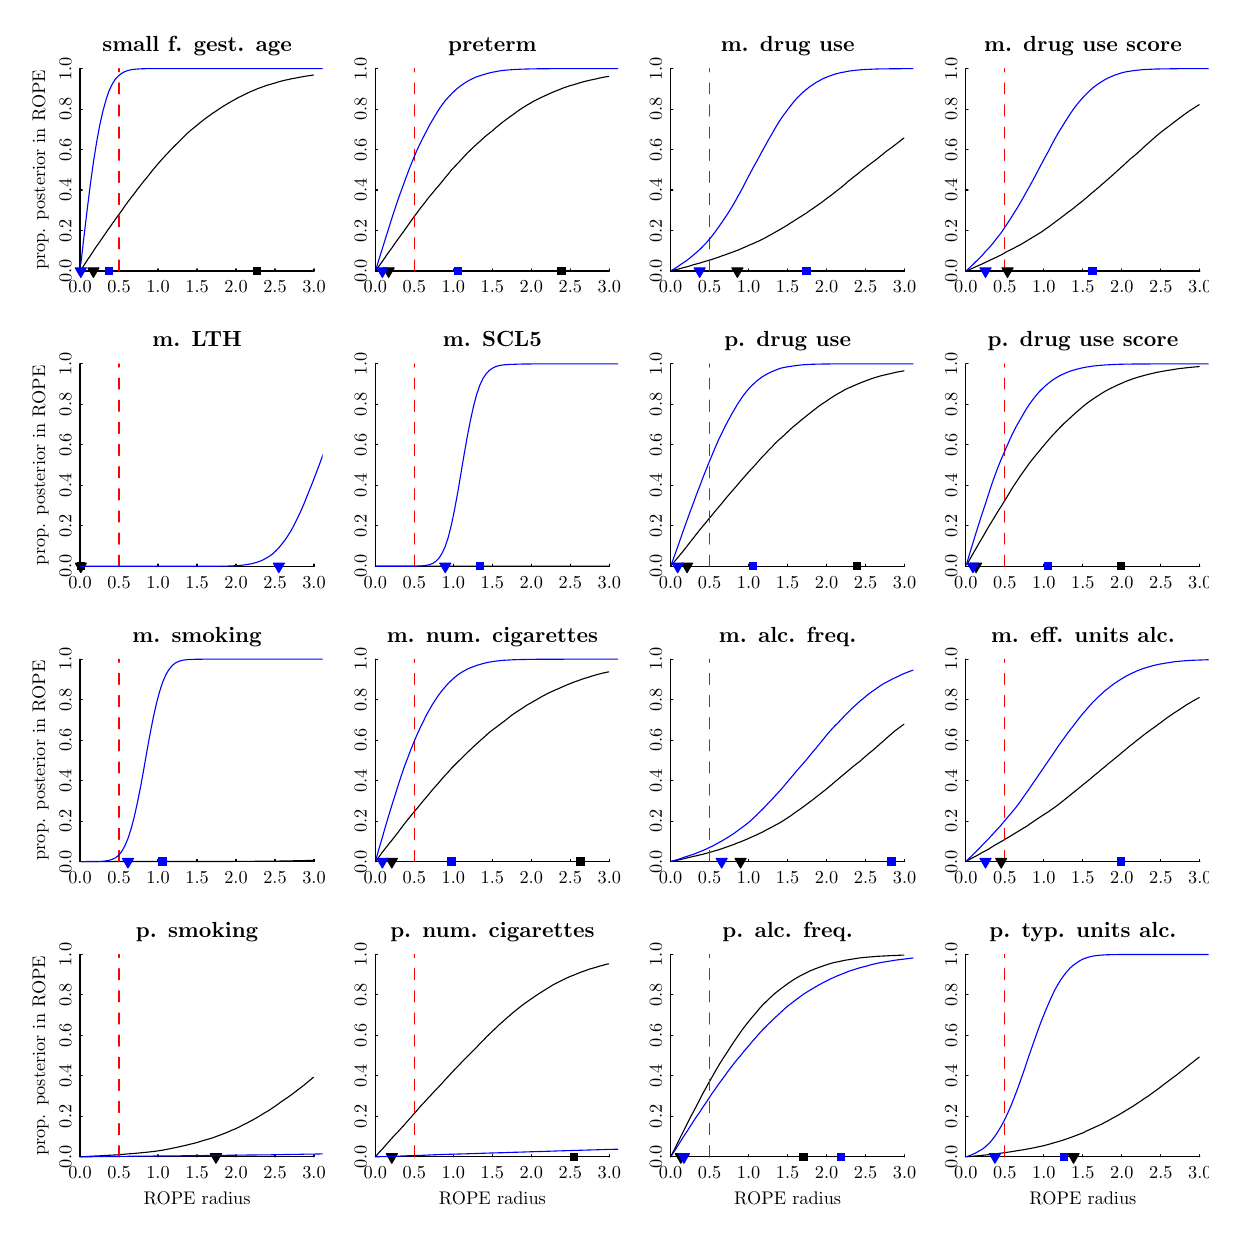
\begin{tikzpicture}[x=1pt,y=1pt]
\definecolor{fillColor}{RGB}{255,255,255}
\path[use as bounding box,fill=fillColor,fill opacity=0.00] (0,0) rectangle (426.79,426.79);
\begin{scope}
\path[clip] ( 15.84,335.93) rectangle (106.62,414.91);
\definecolor{drawColor}{RGB}{0,0,0}

\path[draw=drawColor,line width= 0.4pt,line join=round,line cap=round] ( 19.20,339.21) --
	( 20.34,340.89) --
	( 21.47,342.68) --
	( 22.61,344.35) --
	( 23.75,346.08) --
	( 24.88,347.80) --
	( 26.02,349.38) --
	( 27.15,351.01) --
	( 28.29,352.70) --
	( 29.42,354.34) --
	( 30.56,355.92) --
	( 31.70,357.55) --
	( 32.83,359.13) --
	( 33.97,360.63) --
	( 35.10,362.32) --
	( 36.24,363.87) --
	( 37.38,365.38) --
	( 38.51,366.80) --
	( 39.65,368.37) --
	( 40.78,369.80) --
	( 41.92,371.27) --
	( 43.06,372.59) --
	( 44.19,374.04) --
	( 45.33,375.50) --
	( 46.46,376.84) --
	( 47.60,378.18) --
	( 48.73,379.44) --
	( 49.87,380.68) --
	( 51.01,381.88) --
	( 52.14,383.09) --
	( 53.28,384.26) --
	( 54.41,385.32) --
	( 55.55,386.49) --
	( 56.69,387.62) --
	( 57.82,388.75) --
	( 58.96,389.71) --
	( 60.09,390.65) --
	( 61.23,391.56) --
	( 62.37,392.51) --
	( 63.50,393.40) --
	( 64.64,394.28) --
	( 65.77,395.08) --
	( 66.91,395.91) --
	( 68.04,396.62) --
	( 69.18,397.43) --
	( 70.32,398.15) --
	( 71.45,398.86) --
	( 72.59,399.53) --
	( 73.72,400.19) --
	( 74.86,400.82) --
	( 76.00,401.47) --
	( 77.13,402.02) --
	( 78.27,402.58) --
	( 79.40,403.14) --
	( 80.54,403.68) --
	( 81.67,404.12) --
	( 82.81,404.63) --
	( 83.95,405.06) --
	( 85.08,405.46) --
	( 86.22,405.89) --
	( 87.35,406.22) --
	( 88.49,406.53) --
	( 89.63,406.87) --
	( 90.76,407.23) --
	( 91.90,407.54) --
	( 93.03,407.81) --
	( 94.17,408.04) --
	( 95.31,408.32) --
	( 96.44,408.49) --
	( 97.58,408.74) --
	( 98.71,408.94) --
	( 99.85,409.17) --
	(100.98,409.33) --
	(102.12,409.49) --
	(103.26,409.69);
\end{scope}
\begin{scope}
\path[clip] (  0.00,320.09) rectangle (106.70,426.79);
\definecolor{drawColor}{RGB}{0,0,0}

\node[text=drawColor,rotate= 90.00,anchor=base,inner sep=0pt, outer sep=0pt, scale=  0.66] at (  6.34,375.42) {prop. posterior in ROPE};

\node[text=drawColor,anchor=base,inner sep=0pt, outer sep=0pt, scale=  0.79] at ( 61.23,418.12) {\bfseries small f. gest. age};
\end{scope}
\begin{scope}
\path[clip] (  0.00,  0.00) rectangle (426.79,426.79);
\definecolor{drawColor}{RGB}{0,0,0}

\path[draw=drawColor,line width= 0.4pt,line join=round,line cap=round] ( 18.92,338.86) -- (103.47,338.86);

\path[draw=drawColor,line width= 0.4pt,line join=round,line cap=round] ( 18.92,338.86) -- ( 18.92,339.65);

\path[draw=drawColor,line width= 0.4pt,line join=round,line cap=round] ( 33.01,338.86) -- ( 33.01,339.65);

\path[draw=drawColor,line width= 0.4pt,line join=round,line cap=round] ( 47.10,338.86) -- ( 47.10,339.65);

\path[draw=drawColor,line width= 0.4pt,line join=round,line cap=round] ( 61.20,338.86) -- ( 61.20,339.65);

\path[draw=drawColor,line width= 0.4pt,line join=round,line cap=round] ( 75.29,338.86) -- ( 75.29,339.65);

\path[draw=drawColor,line width= 0.4pt,line join=round,line cap=round] ( 89.38,338.86) -- ( 89.38,339.65);

\path[draw=drawColor,line width= 0.4pt,line join=round,line cap=round] (103.47,338.86) -- (103.47,339.65);

\node[text=drawColor,anchor=base,inner sep=0pt, outer sep=0pt, scale=  0.66] at ( 18.92,330.94) {0.0};

\node[text=drawColor,anchor=base,inner sep=0pt, outer sep=0pt, scale=  0.66] at ( 33.01,330.94) {0.5};

\node[text=drawColor,anchor=base,inner sep=0pt, outer sep=0pt, scale=  0.66] at ( 47.10,330.94) {1.0};

\node[text=drawColor,anchor=base,inner sep=0pt, outer sep=0pt, scale=  0.66] at ( 61.20,330.94) {1.5};

\node[text=drawColor,anchor=base,inner sep=0pt, outer sep=0pt, scale=  0.66] at ( 75.29,330.94) {2.0};

\node[text=drawColor,anchor=base,inner sep=0pt, outer sep=0pt, scale=  0.66] at ( 89.38,330.94) {2.5};

\node[text=drawColor,anchor=base,inner sep=0pt, outer sep=0pt, scale=  0.66] at (103.47,330.94) {3.0};

\path[draw=drawColor,line width= 0.4pt,line join=round,line cap=round] ( 18.92,338.86) -- ( 18.92,411.99);

\path[draw=drawColor,line width= 0.4pt,line join=round,line cap=round] ( 18.92,338.86) -- ( 19.71,338.86);

\path[draw=drawColor,line width= 0.4pt,line join=round,line cap=round] ( 18.92,353.48) -- ( 19.71,353.48);

\path[draw=drawColor,line width= 0.4pt,line join=round,line cap=round] ( 18.92,368.11) -- ( 19.71,368.11);

\path[draw=drawColor,line width= 0.4pt,line join=round,line cap=round] ( 18.92,382.74) -- ( 19.71,382.74);

\path[draw=drawColor,line width= 0.4pt,line join=round,line cap=round] ( 18.92,397.36) -- ( 19.71,397.36);

\path[draw=drawColor,line width= 0.4pt,line join=round,line cap=round] ( 18.92,411.99) -- ( 19.71,411.99);

\node[text=drawColor,rotate= 90.00,anchor=base,inner sep=0pt, outer sep=0pt, scale=  0.66] at ( 15.75,338.86) {0.0};

\node[text=drawColor,rotate= 90.00,anchor=base,inner sep=0pt, outer sep=0pt, scale=  0.66] at ( 15.75,353.48) {0.2};

\node[text=drawColor,rotate= 90.00,anchor=base,inner sep=0pt, outer sep=0pt, scale=  0.66] at ( 15.75,368.11) {0.4};

\node[text=drawColor,rotate= 90.00,anchor=base,inner sep=0pt, outer sep=0pt, scale=  0.66] at ( 15.75,382.74) {0.6};

\node[text=drawColor,rotate= 90.00,anchor=base,inner sep=0pt, outer sep=0pt, scale=  0.66] at ( 15.75,397.36) {0.8};

\node[text=drawColor,rotate= 90.00,anchor=base,inner sep=0pt, outer sep=0pt, scale=  0.66] at ( 15.75,411.99) {1.0};
\end{scope}
\begin{scope}
\path[clip] ( 15.84,335.93) rectangle (106.62,414.91);
\definecolor{drawColor}{RGB}{0,0,0}

\path[draw=drawColor,line width= 0.4pt,line join=round,line cap=round] (131.65,338.86) --
	(131.65,411.99);
\definecolor{drawColor}{RGB}{255,0,0}

\path[draw=drawColor,line width= 0.4pt,dash pattern=on 4pt off 4pt ,line join=round,line cap=round] ( 33.01,338.86) --
	( 33.01,411.99);
\definecolor{fillColor}{RGB}{0,0,0}

\path[fill=fillColor] ( 81.33,337.37) --
	( 84.30,337.37) --
	( 84.30,340.34) --
	( 81.33,340.34) --
	cycle;
\definecolor{drawColor}{RGB}{0,0,0}

\path[draw=drawColor,line width= 0.4pt,line join=round,line cap=round,fill=fillColor] ( 23.75,336.55) --
	( 25.75,340.01) --
	( 21.75,340.01) --
	cycle;
\definecolor{drawColor}{RGB}{0,0,255}

\path[draw=drawColor,line width= 0.4pt,line join=round,line cap=round] ( 19.20,341.27) --
	( 20.34,351.26) --
	( 21.47,360.79) --
	( 22.61,369.87) --
	( 23.75,378.15) --
	( 24.88,385.22) --
	( 26.02,391.44) --
	( 27.15,396.48) --
	( 28.29,400.64) --
	( 29.42,404.01) --
	( 30.56,406.41) --
	( 31.70,408.19) --
	( 32.83,409.41) --
	( 33.97,410.28) --
	( 35.10,410.89) --
	( 36.24,411.32) --
	( 37.38,411.60) --
	( 38.51,411.74) --
	( 39.65,411.84) --
	( 40.78,411.91) --
	( 41.92,411.95) --
	( 43.06,411.98) --
	( 44.19,411.98) --
	( 45.33,411.98) --
	( 46.46,411.98) --
	( 47.60,411.98) --
	( 48.73,411.98) --
	( 49.87,411.99) --
	( 51.01,411.99) --
	( 52.14,411.99) --
	( 53.28,411.99) --
	( 54.41,411.99) --
	( 55.55,411.99) --
	( 56.69,411.99) --
	( 57.82,411.99) --
	( 58.96,411.99) --
	( 60.09,411.99) --
	( 61.23,411.99) --
	( 62.37,411.99) --
	( 63.50,411.99) --
	( 64.64,411.99) --
	( 65.77,411.99) --
	( 66.91,411.99) --
	( 68.04,411.99) --
	( 69.18,411.99) --
	( 70.32,411.99) --
	( 71.45,411.99) --
	( 72.59,411.99) --
	( 73.72,411.99) --
	( 74.86,411.99) --
	( 76.00,411.99) --
	( 77.13,411.99) --
	( 78.27,411.99) --
	( 79.40,411.99) --
	( 80.54,411.99) --
	( 81.67,411.99) --
	( 82.81,411.99) --
	( 83.95,411.99) --
	( 85.08,411.99) --
	( 86.22,411.99) --
	( 87.35,411.99) --
	( 88.49,411.99) --
	( 89.63,411.99) --
	( 90.76,411.99) --
	( 91.90,411.99) --
	( 93.03,411.99) --
	( 94.17,411.99) --
	( 95.31,411.99) --
	( 96.44,411.99) --
	( 97.58,411.99) --
	( 98.71,411.99) --
	( 99.85,411.99) --
	(100.98,411.99) --
	(102.12,411.99) --
	(103.26,411.99) --
	(104.39,411.99) --
	(105.53,411.99) --
	(106.66,411.99) --
	(107.80,411.99) --
	(108.94,411.99) --
	(110.07,411.99) --
	(111.21,411.99) --
	(112.34,411.99) --
	(113.48,411.99) --
	(114.62,411.99) --
	(115.75,411.99) --
	(116.89,411.99) --
	(118.02,411.99) --
	(119.16,411.99) --
	(120.29,411.99) --
	(121.43,411.99) --
	(122.57,411.99) --
	(123.70,411.99) --
	(124.84,411.99) --
	(125.97,411.99) --
	(127.11,411.99) --
	(128.25,411.99) --
	(129.38,411.99) --
	(130.52,411.99) --
	(131.65,411.99);
\definecolor{fillColor}{RGB}{0,0,255}

\path[fill=fillColor] ( 27.94,337.37) --
	( 30.91,337.37) --
	( 30.91,340.34) --
	( 27.94,340.34) --
	cycle;

\path[draw=drawColor,line width= 0.4pt,line join=round,line cap=round,fill=fillColor] ( 19.20,336.55) --
	( 21.20,340.01) --
	( 17.20,340.01) --
	cycle;
\end{scope}
\begin{scope}
\path[clip] (122.54,335.93) rectangle (213.32,414.91);
\definecolor{drawColor}{RGB}{0,0,0}

\path[draw=drawColor,line width= 0.4pt,line join=round,line cap=round] (125.90,339.19) --
	(127.04,340.76) --
	(128.17,342.37) --
	(129.31,344.00) --
	(130.44,345.65) --
	(131.58,347.16) --
	(132.72,348.86) --
	(133.85,350.41) --
	(134.99,351.98) --
	(136.12,353.50) --
	(137.26,355.16) --
	(138.39,356.73) --
	(139.53,358.36) --
	(140.67,359.85) --
	(141.80,361.42) --
	(142.94,362.84) --
	(144.07,364.32) --
	(145.21,365.77) --
	(146.35,367.12) --
	(147.48,368.52) --
	(148.62,369.79) --
	(149.75,371.19) --
	(150.89,372.62) --
	(152.02,373.93) --
	(153.16,375.39) --
	(154.30,376.59) --
	(155.43,377.76) --
	(156.57,378.99) --
	(157.70,380.24) --
	(158.84,381.44) --
	(159.98,382.55) --
	(161.11,383.64) --
	(162.25,384.68) --
	(163.38,385.68) --
	(164.52,386.72) --
	(165.66,387.75) --
	(166.79,388.63) --
	(167.93,389.52) --
	(169.06,390.55) --
	(170.20,391.46) --
	(171.33,392.41) --
	(172.47,393.27) --
	(173.61,394.11) --
	(174.74,394.94) --
	(175.88,395.73) --
	(177.01,396.58) --
	(178.15,397.37) --
	(179.29,398.11) --
	(180.42,398.80) --
	(181.56,399.44) --
	(182.69,400.12) --
	(183.83,400.68) --
	(184.97,401.28) --
	(186.10,401.81) --
	(187.24,402.33) --
	(188.37,402.86) --
	(189.51,403.34) --
	(190.64,403.84) --
	(191.78,404.27) --
	(192.92,404.73) --
	(194.05,405.18) --
	(195.19,405.57) --
	(196.32,405.91) --
	(197.46,406.22) --
	(198.60,406.58) --
	(199.73,406.93) --
	(200.87,407.25) --
	(202.00,407.53) --
	(203.14,407.80) --
	(204.27,408.04) --
	(205.41,408.28) --
	(206.55,408.56) --
	(207.68,408.80) --
	(208.82,409.01) --
	(209.95,409.16);
\end{scope}
\begin{scope}
\path[clip] (106.70,320.09) rectangle (213.40,426.79);
\definecolor{drawColor}{RGB}{0,0,0}

\node[text=drawColor,anchor=base,inner sep=0pt, outer sep=0pt, scale=  0.79] at (167.93,418.12) {\bfseries preterm};
\end{scope}
\begin{scope}
\path[clip] (  0.00,  0.00) rectangle (426.79,426.79);
\definecolor{drawColor}{RGB}{0,0,0}

\path[draw=drawColor,line width= 0.4pt,line join=round,line cap=round] (125.62,338.86) -- (210.17,338.86);

\path[draw=drawColor,line width= 0.4pt,line join=round,line cap=round] (125.62,338.86) -- (125.62,339.65);

\path[draw=drawColor,line width= 0.4pt,line join=round,line cap=round] (139.71,338.86) -- (139.71,339.65);

\path[draw=drawColor,line width= 0.4pt,line join=round,line cap=round] (153.80,338.86) -- (153.80,339.65);

\path[draw=drawColor,line width= 0.4pt,line join=round,line cap=round] (167.89,338.86) -- (167.89,339.65);

\path[draw=drawColor,line width= 0.4pt,line join=round,line cap=round] (181.98,338.86) -- (181.98,339.65);

\path[draw=drawColor,line width= 0.4pt,line join=round,line cap=round] (196.08,338.86) -- (196.08,339.65);

\path[draw=drawColor,line width= 0.4pt,line join=round,line cap=round] (210.17,338.86) -- (210.17,339.65);

\node[text=drawColor,anchor=base,inner sep=0pt, outer sep=0pt, scale=  0.66] at (125.62,330.94) {0.0};

\node[text=drawColor,anchor=base,inner sep=0pt, outer sep=0pt, scale=  0.66] at (139.71,330.94) {0.5};

\node[text=drawColor,anchor=base,inner sep=0pt, outer sep=0pt, scale=  0.66] at (153.80,330.94) {1.0};

\node[text=drawColor,anchor=base,inner sep=0pt, outer sep=0pt, scale=  0.66] at (167.89,330.94) {1.5};

\node[text=drawColor,anchor=base,inner sep=0pt, outer sep=0pt, scale=  0.66] at (181.98,330.94) {2.0};

\node[text=drawColor,anchor=base,inner sep=0pt, outer sep=0pt, scale=  0.66] at (196.08,330.94) {2.5};

\node[text=drawColor,anchor=base,inner sep=0pt, outer sep=0pt, scale=  0.66] at (210.17,330.94) {3.0};

\path[draw=drawColor,line width= 0.4pt,line join=round,line cap=round] (125.62,338.86) -- (125.62,411.99);

\path[draw=drawColor,line width= 0.4pt,line join=round,line cap=round] (125.62,338.86) -- (126.41,338.86);

\path[draw=drawColor,line width= 0.4pt,line join=round,line cap=round] (125.62,353.48) -- (126.41,353.48);

\path[draw=drawColor,line width= 0.4pt,line join=round,line cap=round] (125.62,368.11) -- (126.41,368.11);

\path[draw=drawColor,line width= 0.4pt,line join=round,line cap=round] (125.62,382.74) -- (126.41,382.74);

\path[draw=drawColor,line width= 0.4pt,line join=round,line cap=round] (125.62,397.36) -- (126.41,397.36);

\path[draw=drawColor,line width= 0.4pt,line join=round,line cap=round] (125.62,411.99) -- (126.41,411.99);

\node[text=drawColor,rotate= 90.00,anchor=base,inner sep=0pt, outer sep=0pt, scale=  0.66] at (122.45,338.86) {0.0};

\node[text=drawColor,rotate= 90.00,anchor=base,inner sep=0pt, outer sep=0pt, scale=  0.66] at (122.45,353.48) {0.2};

\node[text=drawColor,rotate= 90.00,anchor=base,inner sep=0pt, outer sep=0pt, scale=  0.66] at (122.45,368.11) {0.4};

\node[text=drawColor,rotate= 90.00,anchor=base,inner sep=0pt, outer sep=0pt, scale=  0.66] at (122.45,382.74) {0.6};

\node[text=drawColor,rotate= 90.00,anchor=base,inner sep=0pt, outer sep=0pt, scale=  0.66] at (122.45,397.36) {0.8};

\node[text=drawColor,rotate= 90.00,anchor=base,inner sep=0pt, outer sep=0pt, scale=  0.66] at (122.45,411.99) {1.0};
\end{scope}
\begin{scope}
\path[clip] (122.54,335.93) rectangle (213.32,414.91);
\definecolor{drawColor}{RGB}{0,0,0}

\path[draw=drawColor,line width= 0.4pt,line join=round,line cap=round] (238.35,338.86) --
	(238.35,411.99);
\definecolor{drawColor}{RGB}{255,0,0}

\path[draw=drawColor,line width= 0.4pt,dash pattern=on 4pt off 4pt ,line join=round,line cap=round] (139.71,338.86) --
	(139.71,411.99);
\definecolor{fillColor}{RGB}{0,0,0}

\path[fill=fillColor] (191.43,337.37) --
	(194.40,337.37) --
	(194.40,340.34) --
	(191.43,340.34) --
	cycle;
\definecolor{drawColor}{RGB}{0,0,0}

\path[draw=drawColor,line width= 0.4pt,line join=round,line cap=round,fill=fillColor] (130.44,336.55) --
	(132.44,340.01) --
	(128.44,340.01) --
	cycle;
\definecolor{drawColor}{RGB}{0,0,255}

\path[draw=drawColor,line width= 0.4pt,line join=round,line cap=round] (125.90,339.68) --
	(127.04,343.34) --
	(128.17,347.00) --
	(129.31,350.66) --
	(130.44,354.20) --
	(131.58,357.88) --
	(132.72,361.39) --
	(133.85,364.72) --
	(134.99,367.88) --
	(136.12,370.99) --
	(137.26,374.07) --
	(138.39,377.01) --
	(139.53,379.81) --
	(140.67,382.49) --
	(141.80,384.88) --
	(142.94,387.21) --
	(144.07,389.32) --
	(145.21,391.53) --
	(146.35,393.53) --
	(147.48,395.42) --
	(148.62,397.27) --
	(149.75,398.92) --
	(150.89,400.39) --
	(152.02,401.65) --
	(153.16,402.86) --
	(154.30,403.97) --
	(155.43,404.98) --
	(156.57,405.87) --
	(157.70,406.63) --
	(158.84,407.36) --
	(159.98,407.97) --
	(161.11,408.54) --
	(162.25,409.03) --
	(163.38,409.41) --
	(164.52,409.77) --
	(165.66,410.11) --
	(166.79,410.41) --
	(167.93,410.68) --
	(169.06,410.88) --
	(170.20,411.11) --
	(171.33,411.27) --
	(172.47,411.41) --
	(173.61,411.51) --
	(174.74,411.59) --
	(175.88,411.65) --
	(177.01,411.71) --
	(178.15,411.78) --
	(179.29,411.82) --
	(180.42,411.85) --
	(181.56,411.88) --
	(182.69,411.90) --
	(183.83,411.92) --
	(184.97,411.94) --
	(186.10,411.95) --
	(187.24,411.95) --
	(188.37,411.96) --
	(189.51,411.97) --
	(190.64,411.97) --
	(191.78,411.97) --
	(192.92,411.98) --
	(194.05,411.98) --
	(195.19,411.98) --
	(196.32,411.98) --
	(197.46,411.98) --
	(198.60,411.98) --
	(199.73,411.98) --
	(200.87,411.98) --
	(202.00,411.98) --
	(203.14,411.98) --
	(204.27,411.98) --
	(205.41,411.99) --
	(206.55,411.99) --
	(207.68,411.99) --
	(208.82,411.99) --
	(209.95,411.99) --
	(211.09,411.99) --
	(212.23,411.99) --
	(213.36,411.99) --
	(214.50,411.99) --
	(215.63,411.99) --
	(216.77,411.99) --
	(217.91,411.99) --
	(219.04,411.99) --
	(220.18,411.99) --
	(221.31,411.99) --
	(222.45,411.99) --
	(223.58,411.99) --
	(224.72,411.99) --
	(225.86,411.99) --
	(226.99,411.99) --
	(228.13,411.99) --
	(229.26,411.99) --
	(230.40,411.99) --
	(231.54,411.99) --
	(232.67,411.99) --
	(233.81,411.99) --
	(234.94,411.99) --
	(236.08,411.99) --
	(237.22,411.99) --
	(238.35,411.99);
\definecolor{fillColor}{RGB}{0,0,255}

\path[fill=fillColor] (153.95,337.37) --
	(156.92,337.37) --
	(156.92,340.34) --
	(153.95,340.34) --
	cycle;

\path[draw=drawColor,line width= 0.4pt,line join=round,line cap=round,fill=fillColor] (128.17,336.55) --
	(130.17,340.01) --
	(126.17,340.01) --
	cycle;
\end{scope}
\begin{scope}
\path[clip] (229.24,335.93) rectangle (320.01,414.91);
\definecolor{drawColor}{RGB}{0,0,0}

\path[draw=drawColor,line width= 0.4pt,line join=round,line cap=round] (232.60,338.94) --
	(233.73,339.24) --
	(234.87,339.50) --
	(236.01,339.80) --
	(237.14,340.12) --
	(238.28,340.40) --
	(239.41,340.74) --
	(240.55,341.12) --
	(241.68,341.41) --
	(242.82,341.72) --
	(243.96,342.07) --
	(245.09,342.41) --
	(246.23,342.74) --
	(247.36,343.08) --
	(248.50,343.48) --
	(249.64,343.85) --
	(250.77,344.28) --
	(251.91,344.66) --
	(253.04,345.08) --
	(254.18,345.49) --
	(255.32,345.92) --
	(256.45,346.33) --
	(257.59,346.81) --
	(258.72,347.31) --
	(259.86,347.79) --
	(260.99,348.33) --
	(262.13,348.76) --
	(263.27,349.30) --
	(264.40,349.78) --
	(265.54,350.37) --
	(266.67,350.95) --
	(267.81,351.59) --
	(268.95,352.20) --
	(270.08,352.86) --
	(271.22,353.52) --
	(272.35,354.15) --
	(273.49,354.82) --
	(274.62,355.50) --
	(275.76,356.26) --
	(276.90,356.96) --
	(278.03,357.70) --
	(279.17,358.40) --
	(280.30,359.11) --
	(281.44,359.84) --
	(282.58,360.68) --
	(283.71,361.42) --
	(284.85,362.24) --
	(285.98,363.01) --
	(287.12,363.81) --
	(288.26,364.71) --
	(289.39,365.56) --
	(290.53,366.37) --
	(291.66,367.29) --
	(292.80,368.16) --
	(293.93,369.03) --
	(295.07,369.99) --
	(296.21,371.02) --
	(297.34,371.91) --
	(298.48,372.85) --
	(299.61,373.69) --
	(300.75,374.65) --
	(301.89,375.56) --
	(303.02,376.44) --
	(304.16,377.30) --
	(305.29,378.16) --
	(306.43,378.98) --
	(307.57,379.91) --
	(308.70,380.81) --
	(309.84,381.77) --
	(310.97,382.61) --
	(312.11,383.43) --
	(313.24,384.28) --
	(314.38,385.18) --
	(315.52,386.05) --
	(316.65,386.94);
\end{scope}
\begin{scope}
\path[clip] (213.40,320.09) rectangle (320.09,426.79);
\definecolor{drawColor}{RGB}{0,0,0}

\node[text=drawColor,anchor=base,inner sep=0pt, outer sep=0pt, scale=  0.79] at (274.62,418.12) {\bfseries m. drug use};
\end{scope}
\begin{scope}
\path[clip] (  0.00,  0.00) rectangle (426.79,426.79);
\definecolor{drawColor}{RGB}{0,0,0}

\path[draw=drawColor,line width= 0.4pt,line join=round,line cap=round] (232.32,338.86) -- (316.87,338.86);

\path[draw=drawColor,line width= 0.4pt,line join=round,line cap=round] (232.32,338.86) -- (232.32,339.65);

\path[draw=drawColor,line width= 0.4pt,line join=round,line cap=round] (246.41,338.86) -- (246.41,339.65);

\path[draw=drawColor,line width= 0.4pt,line join=round,line cap=round] (260.50,338.86) -- (260.50,339.65);

\path[draw=drawColor,line width= 0.4pt,line join=round,line cap=round] (274.59,338.86) -- (274.59,339.65);

\path[draw=drawColor,line width= 0.4pt,line join=round,line cap=round] (288.68,338.86) -- (288.68,339.65);

\path[draw=drawColor,line width= 0.4pt,line join=round,line cap=round] (302.77,338.86) -- (302.77,339.65);

\path[draw=drawColor,line width= 0.4pt,line join=round,line cap=round] (316.87,338.86) -- (316.87,339.65);

\node[text=drawColor,anchor=base,inner sep=0pt, outer sep=0pt, scale=  0.66] at (232.32,330.94) {0.0};

\node[text=drawColor,anchor=base,inner sep=0pt, outer sep=0pt, scale=  0.66] at (246.41,330.94) {0.5};

\node[text=drawColor,anchor=base,inner sep=0pt, outer sep=0pt, scale=  0.66] at (260.50,330.94) {1.0};

\node[text=drawColor,anchor=base,inner sep=0pt, outer sep=0pt, scale=  0.66] at (274.59,330.94) {1.5};

\node[text=drawColor,anchor=base,inner sep=0pt, outer sep=0pt, scale=  0.66] at (288.68,330.94) {2.0};

\node[text=drawColor,anchor=base,inner sep=0pt, outer sep=0pt, scale=  0.66] at (302.77,330.94) {2.5};

\node[text=drawColor,anchor=base,inner sep=0pt, outer sep=0pt, scale=  0.66] at (316.87,330.94) {3.0};

\path[draw=drawColor,line width= 0.4pt,line join=round,line cap=round] (232.32,338.86) -- (232.32,411.99);

\path[draw=drawColor,line width= 0.4pt,line join=round,line cap=round] (232.32,338.86) -- (233.11,338.86);

\path[draw=drawColor,line width= 0.4pt,line join=round,line cap=round] (232.32,353.48) -- (233.11,353.48);

\path[draw=drawColor,line width= 0.4pt,line join=round,line cap=round] (232.32,368.11) -- (233.11,368.11);

\path[draw=drawColor,line width= 0.4pt,line join=round,line cap=round] (232.32,382.74) -- (233.11,382.74);

\path[draw=drawColor,line width= 0.4pt,line join=round,line cap=round] (232.32,397.36) -- (233.11,397.36);

\path[draw=drawColor,line width= 0.4pt,line join=round,line cap=round] (232.32,411.99) -- (233.11,411.99);

\node[text=drawColor,rotate= 90.00,anchor=base,inner sep=0pt, outer sep=0pt, scale=  0.66] at (229.15,338.86) {0.0};

\node[text=drawColor,rotate= 90.00,anchor=base,inner sep=0pt, outer sep=0pt, scale=  0.66] at (229.15,353.48) {0.2};

\node[text=drawColor,rotate= 90.00,anchor=base,inner sep=0pt, outer sep=0pt, scale=  0.66] at (229.15,368.11) {0.4};

\node[text=drawColor,rotate= 90.00,anchor=base,inner sep=0pt, outer sep=0pt, scale=  0.66] at (229.15,382.74) {0.6};

\node[text=drawColor,rotate= 90.00,anchor=base,inner sep=0pt, outer sep=0pt, scale=  0.66] at (229.15,397.36) {0.8};

\node[text=drawColor,rotate= 90.00,anchor=base,inner sep=0pt, outer sep=0pt, scale=  0.66] at (229.15,411.99) {1.0};
\end{scope}
\begin{scope}
\path[clip] (229.24,335.93) rectangle (320.01,414.91);
\definecolor{drawColor}{RGB}{0,0,0}

\path[draw=drawColor,line width= 0.4pt,line join=round,line cap=round] (345.05,338.86) --
	(345.05,411.99);
\definecolor{drawColor}{RGB}{255,0,0}

\path[draw=drawColor,line width= 0.4pt,dash pattern=on 4pt off 4pt ,line join=round,line cap=round] (246.41,338.86) --
	(246.41,411.99);
\definecolor{fillColor}{RGB}{0,0,0}

\path[fill=fillColor] (343.56,337.37) --
	(346.53,337.37) --
	(346.53,340.34) --
	(343.56,340.34) --
	cycle;
\definecolor{drawColor}{RGB}{0,0,0}

\path[draw=drawColor,line width= 0.4pt,line join=round,line cap=round,fill=fillColor] (256.45,336.55) --
	(258.45,340.01) --
	(254.45,340.01) --
	cycle;
\definecolor{drawColor}{RGB}{0,0,255}

\path[draw=drawColor,line width= 0.4pt,line join=round,line cap=round] (232.60,339.05) --
	(233.73,339.69) --
	(234.87,340.42) --
	(236.01,341.25) --
	(237.14,341.99) --
	(238.28,342.77) --
	(239.41,343.67) --
	(240.55,344.61) --
	(241.68,345.58) --
	(242.82,346.60) --
	(243.96,347.75) --
	(245.09,348.91) --
	(246.23,350.20) --
	(247.36,351.59) --
	(248.50,353.11) --
	(249.64,354.68) --
	(250.77,356.33) --
	(251.91,358.01) --
	(253.04,359.69) --
	(254.18,361.54) --
	(255.32,363.41) --
	(256.45,365.49) --
	(257.59,367.49) --
	(258.72,369.61) --
	(259.86,371.89) --
	(260.99,374.02) --
	(262.13,376.19) --
	(263.27,378.19) --
	(264.40,380.26) --
	(265.54,382.41) --
	(266.67,384.41) --
	(267.81,386.51) --
	(268.95,388.41) --
	(270.08,390.42) --
	(271.22,392.34) --
	(272.35,394.08) --
	(273.49,395.65) --
	(274.62,397.19) --
	(275.76,398.64) --
	(276.90,400.10) --
	(278.03,401.41) --
	(279.17,402.51) --
	(280.30,403.59) --
	(281.44,404.51) --
	(282.58,405.43) --
	(283.71,406.18) --
	(284.85,406.96) --
	(285.98,407.58) --
	(287.12,408.23) --
	(288.26,408.73) --
	(289.39,409.20) --
	(290.53,409.59) --
	(291.66,409.98) --
	(292.80,410.28) --
	(293.93,410.56) --
	(295.07,410.75) --
	(296.21,410.99) --
	(297.34,411.17) --
	(298.48,411.30) --
	(299.61,411.44) --
	(300.75,411.55) --
	(301.89,411.63) --
	(303.02,411.69) --
	(304.16,411.74) --
	(305.29,411.79) --
	(306.43,411.84) --
	(307.57,411.87) --
	(308.70,411.89) --
	(309.84,411.91) --
	(310.97,411.92) --
	(312.11,411.93) --
	(313.24,411.94) --
	(314.38,411.95) --
	(315.52,411.96) --
	(316.65,411.97) --
	(317.79,411.97) --
	(318.92,411.98) --
	(320.06,411.98) --
	(321.20,411.98) --
	(322.33,411.98) --
	(323.47,411.99) --
	(324.60,411.99) --
	(325.74,411.99) --
	(326.87,411.99) --
	(328.01,411.99) --
	(329.15,411.99) --
	(330.28,411.99) --
	(331.42,411.99) --
	(332.55,411.99) --
	(333.69,411.99) --
	(334.83,411.99) --
	(335.96,411.99) --
	(337.10,411.99) --
	(338.23,411.99) --
	(339.37,411.99) --
	(340.51,411.99) --
	(341.64,411.99) --
	(342.78,411.99) --
	(343.91,411.99) --
	(345.05,411.99);
\definecolor{fillColor}{RGB}{0,0,255}

\path[fill=fillColor] (279.96,337.37) --
	(282.93,337.37) --
	(282.93,340.34) --
	(279.96,340.34) --
	cycle;

\path[draw=drawColor,line width= 0.4pt,line join=round,line cap=round,fill=fillColor] (242.82,336.55) --
	(244.82,340.01) --
	(240.82,340.01) --
	cycle;
\end{scope}
\begin{scope}
\path[clip] (335.93,335.93) rectangle (426.71,414.91);
\definecolor{drawColor}{RGB}{0,0,0}

\path[draw=drawColor,line width= 0.4pt,line join=round,line cap=round] (339.30,339.00) --
	(340.43,339.43) --
	(341.57,339.93) --
	(342.70,340.43) --
	(343.84,340.96) --
	(344.98,341.44) --
	(346.11,342.01) --
	(347.25,342.53) --
	(348.38,343.07) --
	(349.52,343.60) --
	(350.65,344.12) --
	(351.79,344.68) --
	(352.93,345.35) --
	(354.06,346.00) --
	(355.20,346.55) --
	(356.33,347.09) --
	(357.47,347.73) --
	(358.61,348.30) --
	(359.74,348.95) --
	(360.88,349.65) --
	(362.01,350.34) --
	(363.15,351.04) --
	(364.28,351.71) --
	(365.42,352.41) --
	(366.56,353.12) --
	(367.69,353.95) --
	(368.83,354.71) --
	(369.96,355.57) --
	(371.10,356.42) --
	(372.24,357.27) --
	(373.37,358.12) --
	(374.51,358.97) --
	(375.64,359.89) --
	(376.78,360.69) --
	(377.92,361.54) --
	(379.05,362.50) --
	(380.19,363.38) --
	(381.32,364.28) --
	(382.46,365.23) --
	(383.59,366.21) --
	(384.73,367.21) --
	(385.87,368.13) --
	(387.00,369.09) --
	(388.14,370.13) --
	(389.27,371.07) --
	(390.41,372.09) --
	(391.55,373.05) --
	(392.68,374.08) --
	(393.82,375.11) --
	(394.95,376.17) --
	(396.09,377.13) --
	(397.22,378.23) --
	(398.36,379.30) --
	(399.50,380.20) --
	(400.63,381.15) --
	(401.77,382.16) --
	(402.90,383.22) --
	(404.04,384.30) --
	(405.18,385.28) --
	(406.31,386.27) --
	(407.45,387.28) --
	(408.58,388.25) --
	(409.72,389.18) --
	(410.86,390.05) --
	(411.99,390.89) --
	(413.13,391.76) --
	(414.26,392.64) --
	(415.40,393.51) --
	(416.53,394.34) --
	(417.67,395.21) --
	(418.81,396.01) --
	(419.94,396.83) --
	(421.08,397.53) --
	(422.21,398.28) --
	(423.35,398.98);
\end{scope}
\begin{scope}
\path[clip] (320.09,320.09) rectangle (426.79,426.79);
\definecolor{drawColor}{RGB}{0,0,0}

\node[text=drawColor,anchor=base,inner sep=0pt, outer sep=0pt, scale=  0.79] at (381.32,418.12) {\bfseries m. drug use score};
\end{scope}
\begin{scope}
\path[clip] (  0.00,  0.00) rectangle (426.79,426.79);
\definecolor{drawColor}{RGB}{0,0,0}

\path[draw=drawColor,line width= 0.4pt,line join=round,line cap=round] (339.01,338.86) -- (423.56,338.86);

\path[draw=drawColor,line width= 0.4pt,line join=round,line cap=round] (339.01,338.86) -- (339.01,339.65);

\path[draw=drawColor,line width= 0.4pt,line join=round,line cap=round] (353.11,338.86) -- (353.11,339.65);

\path[draw=drawColor,line width= 0.4pt,line join=round,line cap=round] (367.20,338.86) -- (367.20,339.65);

\path[draw=drawColor,line width= 0.4pt,line join=round,line cap=round] (381.29,338.86) -- (381.29,339.65);

\path[draw=drawColor,line width= 0.4pt,line join=round,line cap=round] (395.38,338.86) -- (395.38,339.65);

\path[draw=drawColor,line width= 0.4pt,line join=round,line cap=round] (409.47,338.86) -- (409.47,339.65);

\path[draw=drawColor,line width= 0.4pt,line join=round,line cap=round] (423.56,338.86) -- (423.56,339.65);

\node[text=drawColor,anchor=base,inner sep=0pt, outer sep=0pt, scale=  0.66] at (339.01,330.94) {0.0};

\node[text=drawColor,anchor=base,inner sep=0pt, outer sep=0pt, scale=  0.66] at (353.11,330.94) {0.5};

\node[text=drawColor,anchor=base,inner sep=0pt, outer sep=0pt, scale=  0.66] at (367.20,330.94) {1.0};

\node[text=drawColor,anchor=base,inner sep=0pt, outer sep=0pt, scale=  0.66] at (381.29,330.94) {1.5};

\node[text=drawColor,anchor=base,inner sep=0pt, outer sep=0pt, scale=  0.66] at (395.38,330.94) {2.0};

\node[text=drawColor,anchor=base,inner sep=0pt, outer sep=0pt, scale=  0.66] at (409.47,330.94) {2.5};

\node[text=drawColor,anchor=base,inner sep=0pt, outer sep=0pt, scale=  0.66] at (423.56,330.94) {3.0};

\path[draw=drawColor,line width= 0.4pt,line join=round,line cap=round] (339.01,338.86) -- (339.01,411.99);

\path[draw=drawColor,line width= 0.4pt,line join=round,line cap=round] (339.01,338.86) -- (339.80,338.86);

\path[draw=drawColor,line width= 0.4pt,line join=round,line cap=round] (339.01,353.48) -- (339.80,353.48);

\path[draw=drawColor,line width= 0.4pt,line join=round,line cap=round] (339.01,368.11) -- (339.80,368.11);

\path[draw=drawColor,line width= 0.4pt,line join=round,line cap=round] (339.01,382.74) -- (339.80,382.74);

\path[draw=drawColor,line width= 0.4pt,line join=round,line cap=round] (339.01,397.36) -- (339.80,397.36);

\path[draw=drawColor,line width= 0.4pt,line join=round,line cap=round] (339.01,411.99) -- (339.80,411.99);

\node[text=drawColor,rotate= 90.00,anchor=base,inner sep=0pt, outer sep=0pt, scale=  0.66] at (335.85,338.86) {0.0};

\node[text=drawColor,rotate= 90.00,anchor=base,inner sep=0pt, outer sep=0pt, scale=  0.66] at (335.85,353.48) {0.2};

\node[text=drawColor,rotate= 90.00,anchor=base,inner sep=0pt, outer sep=0pt, scale=  0.66] at (335.85,368.11) {0.4};

\node[text=drawColor,rotate= 90.00,anchor=base,inner sep=0pt, outer sep=0pt, scale=  0.66] at (335.85,382.74) {0.6};

\node[text=drawColor,rotate= 90.00,anchor=base,inner sep=0pt, outer sep=0pt, scale=  0.66] at (335.85,397.36) {0.8};

\node[text=drawColor,rotate= 90.00,anchor=base,inner sep=0pt, outer sep=0pt, scale=  0.66] at (335.85,411.99) {1.0};
\end{scope}
\begin{scope}
\path[clip] (335.93,335.93) rectangle (426.71,414.91);
\definecolor{drawColor}{RGB}{255,0,0}

\path[draw=drawColor,line width= 0.4pt,dash pattern=on 4pt off 4pt ,line join=round,line cap=round] (353.11,338.86) --
	(353.11,411.99);
\definecolor{drawColor}{RGB}{0,0,0}
\definecolor{fillColor}{RGB}{0,0,0}

\path[draw=drawColor,line width= 0.4pt,line join=round,line cap=round,fill=fillColor] (354.06,336.55) --
	(356.06,340.01) --
	(352.06,340.01) --
	cycle;
\definecolor{drawColor}{RGB}{0,0,255}

\path[draw=drawColor,line width= 0.4pt,line join=round,line cap=round] (339.30,339.10) --
	(340.43,340.12) --
	(341.57,341.20) --
	(342.70,342.31) --
	(343.84,343.44) --
	(344.98,344.57) --
	(346.11,345.93) --
	(347.25,347.09) --
	(348.38,348.36) --
	(349.52,349.81) --
	(350.65,351.28) --
	(351.79,352.71) --
	(352.93,354.38) --
	(354.06,356.09) --
	(355.20,357.84) --
	(356.33,359.68) --
	(357.47,361.47) --
	(358.61,363.41) --
	(359.74,365.36) --
	(360.88,367.45) --
	(362.01,369.42) --
	(363.15,371.50) --
	(364.28,373.62) --
	(365.42,375.82) --
	(366.56,377.93) --
	(367.69,380.07) --
	(368.83,382.11) --
	(369.96,384.34) --
	(371.10,386.45) --
	(372.24,388.52) --
	(373.37,390.35) --
	(374.51,392.15) --
	(375.64,393.96) --
	(376.78,395.74) --
	(377.92,397.40) --
	(379.05,398.89) --
	(380.19,400.28) --
	(381.32,401.54) --
	(382.46,402.75) --
	(383.59,403.86) --
	(384.73,404.90) --
	(385.87,405.81) --
	(387.00,406.60) --
	(388.14,407.31) --
	(389.27,408.00) --
	(390.41,408.61) --
	(391.55,409.12) --
	(392.68,409.58) --
	(393.82,409.99) --
	(394.95,410.36) --
	(396.09,410.65) --
	(397.22,410.90) --
	(398.36,411.07) --
	(399.50,411.24) --
	(400.63,411.38) --
	(401.77,411.50) --
	(402.90,411.61) --
	(404.04,411.69) --
	(405.18,411.73) --
	(406.31,411.78) --
	(407.45,411.84) --
	(408.58,411.86) --
	(409.72,411.88) --
	(410.86,411.90) --
	(411.99,411.91) --
	(413.13,411.93) --
	(414.26,411.95) --
	(415.40,411.96) --
	(416.53,411.97) --
	(417.67,411.98) --
	(418.81,411.98) --
	(419.94,411.98) --
	(421.08,411.98) --
	(422.21,411.98) --
	(423.35,411.98) --
	(424.49,411.98) --
	(425.62,411.98) --
	(426.76,411.99) --
	(426.79,411.99);
\definecolor{fillColor}{RGB}{0,0,255}

\path[fill=fillColor] (383.25,337.37) --
	(386.22,337.37) --
	(386.22,340.34) --
	(383.25,340.34) --
	cycle;

\path[draw=drawColor,line width= 0.4pt,line join=round,line cap=round,fill=fillColor] (346.11,336.55) --
	(348.11,340.01) --
	(344.11,340.01) --
	cycle;
\end{scope}
\begin{scope}
\path[clip] ( 15.84,229.24) rectangle (106.62,308.21);
\definecolor{drawColor}{RGB}{0,0,0}

\path[draw=drawColor,line width= 0.4pt,line join=round,line cap=round] ( 19.20,232.16) --
	( 20.34,232.16) --
	( 21.47,232.16) --
	( 22.61,232.16) --
	( 23.75,232.16) --
	( 24.88,232.16) --
	( 26.02,232.16) --
	( 27.15,232.16) --
	( 28.29,232.16) --
	( 29.42,232.16) --
	( 30.56,232.16) --
	( 31.70,232.16) --
	( 32.83,232.16) --
	( 33.97,232.16) --
	( 35.10,232.16) --
	( 36.24,232.16) --
	( 37.38,232.16) --
	( 38.51,232.16) --
	( 39.65,232.16) --
	( 40.78,232.16) --
	( 41.92,232.16) --
	( 43.06,232.16) --
	( 44.19,232.16) --
	( 45.33,232.16) --
	( 46.46,232.16) --
	( 47.60,232.16) --
	( 48.73,232.16) --
	( 49.87,232.16) --
	( 51.01,232.16) --
	( 52.14,232.16) --
	( 53.28,232.16) --
	( 54.41,232.16) --
	( 55.55,232.16) --
	( 56.69,232.16) --
	( 57.82,232.16) --
	( 58.96,232.16) --
	( 60.09,232.16) --
	( 61.23,232.16) --
	( 62.37,232.16) --
	( 63.50,232.16) --
	( 64.64,232.16) --
	( 65.77,232.16) --
	( 66.91,232.16) --
	( 68.04,232.16) --
	( 69.18,232.16) --
	( 70.32,232.16) --
	( 71.45,232.16) --
	( 72.59,232.16) --
	( 73.72,232.16) --
	( 74.86,232.16) --
	( 76.00,232.16) --
	( 77.13,232.16) --
	( 78.27,232.16) --
	( 79.40,232.16) --
	( 80.54,232.16) --
	( 81.67,232.16) --
	( 82.81,232.16) --
	( 83.95,232.16) --
	( 85.08,232.16) --
	( 86.22,232.16) --
	( 87.35,232.16) --
	( 88.49,232.16) --
	( 89.63,232.16) --
	( 90.76,232.16) --
	( 91.90,232.16) --
	( 93.03,232.16) --
	( 94.17,232.16) --
	( 95.31,232.16) --
	( 96.44,232.16) --
	( 97.58,232.16) --
	( 98.71,232.16) --
	( 99.85,232.16) --
	(100.98,232.16) --
	(102.12,232.16) --
	(103.26,232.16);
\end{scope}
\begin{scope}
\path[clip] (  0.00,213.40) rectangle (106.70,320.09);
\definecolor{drawColor}{RGB}{0,0,0}

\node[text=drawColor,rotate= 90.00,anchor=base,inner sep=0pt, outer sep=0pt, scale=  0.66] at (  6.34,268.72) {prop. posterior in ROPE};

\node[text=drawColor,anchor=base,inner sep=0pt, outer sep=0pt, scale=  0.79] at ( 61.23,311.42) {\bfseries m. LTH};
\end{scope}
\begin{scope}
\path[clip] (  0.00,  0.00) rectangle (426.79,426.79);
\definecolor{drawColor}{RGB}{0,0,0}

\path[draw=drawColor,line width= 0.4pt,line join=round,line cap=round] ( 18.92,232.16) -- (103.47,232.16);

\path[draw=drawColor,line width= 0.4pt,line join=round,line cap=round] ( 18.92,232.16) -- ( 18.92,232.95);

\path[draw=drawColor,line width= 0.4pt,line join=round,line cap=round] ( 33.01,232.16) -- ( 33.01,232.95);

\path[draw=drawColor,line width= 0.4pt,line join=round,line cap=round] ( 47.10,232.16) -- ( 47.10,232.95);

\path[draw=drawColor,line width= 0.4pt,line join=round,line cap=round] ( 61.20,232.16) -- ( 61.20,232.95);

\path[draw=drawColor,line width= 0.4pt,line join=round,line cap=round] ( 75.29,232.16) -- ( 75.29,232.95);

\path[draw=drawColor,line width= 0.4pt,line join=round,line cap=round] ( 89.38,232.16) -- ( 89.38,232.95);

\path[draw=drawColor,line width= 0.4pt,line join=round,line cap=round] (103.47,232.16) -- (103.47,232.95);

\node[text=drawColor,anchor=base,inner sep=0pt, outer sep=0pt, scale=  0.66] at ( 18.92,224.24) {0.0};

\node[text=drawColor,anchor=base,inner sep=0pt, outer sep=0pt, scale=  0.66] at ( 33.01,224.24) {0.5};

\node[text=drawColor,anchor=base,inner sep=0pt, outer sep=0pt, scale=  0.66] at ( 47.10,224.24) {1.0};

\node[text=drawColor,anchor=base,inner sep=0pt, outer sep=0pt, scale=  0.66] at ( 61.20,224.24) {1.5};

\node[text=drawColor,anchor=base,inner sep=0pt, outer sep=0pt, scale=  0.66] at ( 75.29,224.24) {2.0};

\node[text=drawColor,anchor=base,inner sep=0pt, outer sep=0pt, scale=  0.66] at ( 89.38,224.24) {2.5};

\node[text=drawColor,anchor=base,inner sep=0pt, outer sep=0pt, scale=  0.66] at (103.47,224.24) {3.0};

\path[draw=drawColor,line width= 0.4pt,line join=round,line cap=round] ( 18.92,232.16) -- ( 18.92,305.29);

\path[draw=drawColor,line width= 0.4pt,line join=round,line cap=round] ( 18.92,232.16) -- ( 19.71,232.16);

\path[draw=drawColor,line width= 0.4pt,line join=round,line cap=round] ( 18.92,246.79) -- ( 19.71,246.79);

\path[draw=drawColor,line width= 0.4pt,line join=round,line cap=round] ( 18.92,261.41) -- ( 19.71,261.41);

\path[draw=drawColor,line width= 0.4pt,line join=round,line cap=round] ( 18.92,276.04) -- ( 19.71,276.04);

\path[draw=drawColor,line width= 0.4pt,line join=round,line cap=round] ( 18.92,290.66) -- ( 19.71,290.66);

\path[draw=drawColor,line width= 0.4pt,line join=round,line cap=round] ( 18.92,305.29) -- ( 19.71,305.29);

\node[text=drawColor,rotate= 90.00,anchor=base,inner sep=0pt, outer sep=0pt, scale=  0.66] at ( 15.75,232.16) {0.0};

\node[text=drawColor,rotate= 90.00,anchor=base,inner sep=0pt, outer sep=0pt, scale=  0.66] at ( 15.75,246.79) {0.2};

\node[text=drawColor,rotate= 90.00,anchor=base,inner sep=0pt, outer sep=0pt, scale=  0.66] at ( 15.75,261.41) {0.4};

\node[text=drawColor,rotate= 90.00,anchor=base,inner sep=0pt, outer sep=0pt, scale=  0.66] at ( 15.75,276.04) {0.6};

\node[text=drawColor,rotate= 90.00,anchor=base,inner sep=0pt, outer sep=0pt, scale=  0.66] at ( 15.75,290.66) {0.8};

\node[text=drawColor,rotate= 90.00,anchor=base,inner sep=0pt, outer sep=0pt, scale=  0.66] at ( 15.75,305.29) {1.0};
\end{scope}
\begin{scope}
\path[clip] ( 15.84,229.24) rectangle (106.62,308.21);
\definecolor{drawColor}{RGB}{0,0,0}

\path[draw=drawColor,line width= 0.4pt,line join=round,line cap=round] (131.65,232.16) --
	(131.65,305.29);
\definecolor{drawColor}{RGB}{255,0,0}

\path[draw=drawColor,line width= 0.4pt,dash pattern=on 4pt off 4pt ,line join=round,line cap=round] ( 33.01,232.16) --
	( 33.01,305.29);
\definecolor{fillColor}{RGB}{0,0,0}

\path[fill=fillColor] ( 17.72,230.68) --
	( 20.69,230.68) --
	( 20.69,233.65) --
	( 17.72,233.65) --
	cycle;
\definecolor{drawColor}{RGB}{0,0,0}

\path[draw=drawColor,line width= 0.4pt,line join=round,line cap=round,fill=fillColor] ( 19.20,229.85) --
	( 21.20,233.32) --
	( 17.20,233.32) --
	cycle;
\definecolor{drawColor}{RGB}{0,0,255}

\path[draw=drawColor,line width= 0.4pt,line join=round,line cap=round] ( 19.20,232.16) --
	( 20.34,232.16) --
	( 21.47,232.16) --
	( 22.61,232.16) --
	( 23.75,232.16) --
	( 24.88,232.16) --
	( 26.02,232.16) --
	( 27.15,232.16) --
	( 28.29,232.16) --
	( 29.42,232.16) --
	( 30.56,232.16) --
	( 31.70,232.16) --
	( 32.83,232.16) --
	( 33.97,232.16) --
	( 35.10,232.16) --
	( 36.24,232.16) --
	( 37.38,232.16) --
	( 38.51,232.16) --
	( 39.65,232.16) --
	( 40.78,232.16) --
	( 41.92,232.16) --
	( 43.06,232.16) --
	( 44.19,232.16) --
	( 45.33,232.16) --
	( 46.46,232.16) --
	( 47.60,232.16) --
	( 48.73,232.16) --
	( 49.87,232.16) --
	( 51.01,232.16) --
	( 52.14,232.16) --
	( 53.28,232.16) --
	( 54.41,232.16) --
	( 55.55,232.16) --
	( 56.69,232.16) --
	( 57.82,232.16) --
	( 58.96,232.16) --
	( 60.09,232.16) --
	( 61.23,232.17) --
	( 62.37,232.17) --
	( 63.50,232.17) --
	( 64.64,232.17) --
	( 65.77,232.17) --
	( 66.91,232.18) --
	( 68.04,232.19) --
	( 69.18,232.19) --
	( 70.32,232.20) --
	( 71.45,232.22) --
	( 72.59,232.25) --
	( 73.72,232.31) --
	( 74.86,232.35) --
	( 76.00,232.42) --
	( 77.13,232.51) --
	( 78.27,232.66) --
	( 79.40,232.83) --
	( 80.54,233.00) --
	( 81.67,233.28) --
	( 82.81,233.60) --
	( 83.95,233.99) --
	( 85.08,234.49) --
	( 86.22,235.12) --
	( 87.35,235.80) --
	( 88.49,236.65) --
	( 89.63,237.67) --
	( 90.76,238.86) --
	( 91.90,240.25) --
	( 93.03,241.71) --
	( 94.17,243.41) --
	( 95.31,245.27) --
	( 96.44,247.42) --
	( 97.58,249.76) --
	( 98.71,252.12) --
	( 99.85,254.78) --
	(100.98,257.59) --
	(102.12,260.43) --
	(103.26,263.26) --
	(104.39,266.26) --
	(105.53,269.22) --
	(106.66,272.41) --
	(107.80,275.43) --
	(108.94,278.34) --
	(110.07,281.28) --
	(111.21,283.93) --
	(112.34,286.60) --
	(113.48,289.00) --
	(114.62,291.13) --
	(115.75,293.16) --
	(116.89,295.03) --
	(118.02,296.56) --
	(119.16,297.99) --
	(120.29,299.26) --
	(121.43,300.39) --
	(122.57,301.29) --
	(123.70,302.10) --
	(124.84,302.75) --
	(125.97,303.31) --
	(127.11,303.74) --
	(128.25,304.08) --
	(129.38,304.40) --
	(130.52,304.59) --
	(131.65,304.79);
\definecolor{fillColor}{RGB}{0,0,255}

\path[fill=fillColor] (117.67,230.68) --
	(120.64,230.68) --
	(120.64,233.65) --
	(117.67,233.65) --
	cycle;

\path[draw=drawColor,line width= 0.4pt,line join=round,line cap=round,fill=fillColor] ( 90.76,229.85) --
	( 92.76,233.32) --
	( 88.76,233.32) --
	cycle;
\end{scope}
\begin{scope}
\path[clip] (122.54,229.24) rectangle (213.32,308.21);
\definecolor{drawColor}{RGB}{0,0,0}

\path[draw=drawColor,line width= 0.4pt,line join=round,line cap=round] (125.90,232.16) --
	(127.04,232.16) --
	(128.17,232.16) --
	(129.31,232.16) --
	(130.44,232.16) --
	(131.58,232.16) --
	(132.72,232.16) --
	(133.85,232.16) --
	(134.99,232.16) --
	(136.12,232.16) --
	(137.26,232.16) --
	(138.39,232.16) --
	(139.53,232.16) --
	(140.67,232.16) --
	(141.80,232.16) --
	(142.94,232.16) --
	(144.07,232.16) --
	(145.21,232.16) --
	(146.35,232.16) --
	(147.48,232.16) --
	(148.62,232.16) --
	(149.75,232.16) --
	(150.89,232.16) --
	(152.02,232.16) --
	(153.16,232.16) --
	(154.30,232.16) --
	(155.43,232.16) --
	(156.57,232.16) --
	(157.70,232.16) --
	(158.84,232.16) --
	(159.98,232.16) --
	(161.11,232.16) --
	(162.25,232.16) --
	(163.38,232.16) --
	(164.52,232.16) --
	(165.66,232.16) --
	(166.79,232.16) --
	(167.93,232.16) --
	(169.06,232.16) --
	(170.20,232.16) --
	(171.33,232.16) --
	(172.47,232.16) --
	(173.61,232.16) --
	(174.74,232.16) --
	(175.88,232.16) --
	(177.01,232.16) --
	(178.15,232.16) --
	(179.29,232.16) --
	(180.42,232.16) --
	(181.56,232.16) --
	(182.69,232.16) --
	(183.83,232.16) --
	(184.97,232.16) --
	(186.10,232.16) --
	(187.24,232.16) --
	(188.37,232.16) --
	(189.51,232.16) --
	(190.64,232.16) --
	(191.78,232.16) --
	(192.92,232.16) --
	(194.05,232.16) --
	(195.19,232.17) --
	(196.32,232.17) --
	(197.46,232.17) --
	(198.60,232.17) --
	(199.73,232.17) --
	(200.87,232.17) --
	(202.00,232.17) --
	(203.14,232.17) --
	(204.27,232.17) --
	(205.41,232.17) --
	(206.55,232.17) --
	(207.68,232.17) --
	(208.82,232.17) --
	(209.95,232.17);
\end{scope}
\begin{scope}
\path[clip] (106.70,213.40) rectangle (213.40,320.09);
\definecolor{drawColor}{RGB}{0,0,0}

\node[text=drawColor,anchor=base,inner sep=0pt, outer sep=0pt, scale=  0.79] at (167.93,311.42) {\bfseries m. SCL5};
\end{scope}
\begin{scope}
\path[clip] (  0.00,  0.00) rectangle (426.79,426.79);
\definecolor{drawColor}{RGB}{0,0,0}

\path[draw=drawColor,line width= 0.4pt,line join=round,line cap=round] (125.62,232.16) -- (210.17,232.16);

\path[draw=drawColor,line width= 0.4pt,line join=round,line cap=round] (125.62,232.16) -- (125.62,232.95);

\path[draw=drawColor,line width= 0.4pt,line join=round,line cap=round] (139.71,232.16) -- (139.71,232.95);

\path[draw=drawColor,line width= 0.4pt,line join=round,line cap=round] (153.80,232.16) -- (153.80,232.95);

\path[draw=drawColor,line width= 0.4pt,line join=round,line cap=round] (167.89,232.16) -- (167.89,232.95);

\path[draw=drawColor,line width= 0.4pt,line join=round,line cap=round] (181.98,232.16) -- (181.98,232.95);

\path[draw=drawColor,line width= 0.4pt,line join=round,line cap=round] (196.08,232.16) -- (196.08,232.95);

\path[draw=drawColor,line width= 0.4pt,line join=round,line cap=round] (210.17,232.16) -- (210.17,232.95);

\node[text=drawColor,anchor=base,inner sep=0pt, outer sep=0pt, scale=  0.66] at (125.62,224.24) {0.0};

\node[text=drawColor,anchor=base,inner sep=0pt, outer sep=0pt, scale=  0.66] at (139.71,224.24) {0.5};

\node[text=drawColor,anchor=base,inner sep=0pt, outer sep=0pt, scale=  0.66] at (153.80,224.24) {1.0};

\node[text=drawColor,anchor=base,inner sep=0pt, outer sep=0pt, scale=  0.66] at (167.89,224.24) {1.5};

\node[text=drawColor,anchor=base,inner sep=0pt, outer sep=0pt, scale=  0.66] at (181.98,224.24) {2.0};

\node[text=drawColor,anchor=base,inner sep=0pt, outer sep=0pt, scale=  0.66] at (196.08,224.24) {2.5};

\node[text=drawColor,anchor=base,inner sep=0pt, outer sep=0pt, scale=  0.66] at (210.17,224.24) {3.0};

\path[draw=drawColor,line width= 0.4pt,line join=round,line cap=round] (125.62,232.16) -- (125.62,305.29);

\path[draw=drawColor,line width= 0.4pt,line join=round,line cap=round] (125.62,232.16) -- (126.41,232.16);

\path[draw=drawColor,line width= 0.4pt,line join=round,line cap=round] (125.62,246.79) -- (126.41,246.79);

\path[draw=drawColor,line width= 0.4pt,line join=round,line cap=round] (125.62,261.41) -- (126.41,261.41);

\path[draw=drawColor,line width= 0.4pt,line join=round,line cap=round] (125.62,276.04) -- (126.41,276.04);

\path[draw=drawColor,line width= 0.4pt,line join=round,line cap=round] (125.62,290.66) -- (126.41,290.66);

\path[draw=drawColor,line width= 0.4pt,line join=round,line cap=round] (125.62,305.29) -- (126.41,305.29);

\node[text=drawColor,rotate= 90.00,anchor=base,inner sep=0pt, outer sep=0pt, scale=  0.66] at (122.45,232.16) {0.0};

\node[text=drawColor,rotate= 90.00,anchor=base,inner sep=0pt, outer sep=0pt, scale=  0.66] at (122.45,246.79) {0.2};

\node[text=drawColor,rotate= 90.00,anchor=base,inner sep=0pt, outer sep=0pt, scale=  0.66] at (122.45,261.41) {0.4};

\node[text=drawColor,rotate= 90.00,anchor=base,inner sep=0pt, outer sep=0pt, scale=  0.66] at (122.45,276.04) {0.6};

\node[text=drawColor,rotate= 90.00,anchor=base,inner sep=0pt, outer sep=0pt, scale=  0.66] at (122.45,290.66) {0.8};

\node[text=drawColor,rotate= 90.00,anchor=base,inner sep=0pt, outer sep=0pt, scale=  0.66] at (122.45,305.29) {1.0};
\end{scope}
\begin{scope}
\path[clip] (122.54,229.24) rectangle (213.32,308.21);
\definecolor{drawColor}{RGB}{0,0,0}

\path[draw=drawColor,line width= 0.4pt,line join=round,line cap=round] (238.35,232.16) --
	(238.35,305.29);
\definecolor{drawColor}{RGB}{255,0,0}

\path[draw=drawColor,line width= 0.4pt,dash pattern=on 4pt off 4pt ,line join=round,line cap=round] (139.71,232.16) --
	(139.71,305.29);
\definecolor{fillColor}{RGB}{0,0,0}

\path[fill=fillColor] (236.87,230.68) --
	(239.84,230.68) --
	(239.84,233.65) --
	(236.87,233.65) --
	cycle;
\definecolor{drawColor}{RGB}{0,0,0}

\path[draw=drawColor,line width= 0.4pt,line join=round,line cap=round,fill=fillColor] (238.35,229.85) --
	(240.35,233.32) --
	(236.35,233.32) --
	cycle;
\definecolor{drawColor}{RGB}{0,0,255}

\path[draw=drawColor,line width= 0.4pt,line join=round,line cap=round] (125.90,232.16) --
	(127.04,232.16) --
	(128.17,232.16) --
	(129.31,232.16) --
	(130.44,232.16) --
	(131.58,232.16) --
	(132.72,232.16) --
	(133.85,232.16) --
	(134.99,232.16) --
	(136.12,232.17) --
	(137.26,232.17) --
	(138.39,232.18) --
	(139.53,232.19) --
	(140.67,232.23) --
	(141.80,232.26) --
	(142.94,232.35) --
	(144.07,232.51) --
	(145.21,232.76) --
	(146.35,233.18) --
	(147.48,233.94) --
	(148.62,235.09) --
	(149.75,236.88) --
	(150.89,239.32) --
	(152.02,242.78) --
	(153.16,247.36) --
	(154.30,252.89) --
	(155.43,259.01) --
	(156.57,265.85) --
	(157.70,272.48) --
	(158.84,279.01) --
	(159.98,284.82) --
	(161.11,289.98) --
	(162.25,294.27) --
	(163.38,297.59) --
	(164.52,300.02) --
	(165.66,301.73) --
	(166.79,302.91) --
	(167.93,303.73) --
	(169.06,304.30) --
	(170.20,304.65) --
	(171.33,304.86) --
	(172.47,304.99) --
	(173.61,305.07) --
	(174.74,305.12) --
	(175.88,305.15) --
	(177.01,305.20) --
	(178.15,305.23) --
	(179.29,305.25) --
	(180.42,305.26) --
	(181.56,305.27) --
	(182.69,305.28) --
	(183.83,305.28) --
	(184.97,305.29) --
	(186.10,305.29) --
	(187.24,305.29) --
	(188.37,305.29) --
	(189.51,305.29) --
	(190.64,305.29) --
	(191.78,305.29) --
	(192.92,305.29) --
	(194.05,305.29) --
	(195.19,305.29) --
	(196.32,305.29) --
	(197.46,305.29) --
	(198.60,305.29) --
	(199.73,305.29) --
	(200.87,305.29) --
	(202.00,305.29) --
	(203.14,305.29) --
	(204.27,305.29) --
	(205.41,305.29) --
	(206.55,305.29) --
	(207.68,305.29) --
	(208.82,305.29) --
	(209.95,305.29) --
	(211.09,305.29) --
	(212.23,305.29) --
	(213.36,305.29) --
	(214.50,305.29) --
	(215.63,305.29) --
	(216.77,305.29) --
	(217.91,305.29) --
	(219.04,305.29) --
	(220.18,305.29) --
	(221.31,305.29) --
	(222.45,305.29) --
	(223.58,305.29) --
	(224.72,305.29) --
	(225.86,305.29) --
	(226.99,305.29) --
	(228.13,305.29) --
	(229.26,305.29) --
	(230.40,305.29) --
	(231.54,305.29) --
	(232.67,305.29) --
	(233.81,305.29) --
	(234.94,305.29) --
	(236.08,305.29) --
	(237.22,305.29) --
	(238.35,305.29);
\definecolor{fillColor}{RGB}{0,0,255}

\path[fill=fillColor] (161.90,230.68) --
	(164.87,230.68) --
	(164.87,233.65) --
	(161.90,233.65) --
	cycle;

\path[draw=drawColor,line width= 0.4pt,line join=round,line cap=round,fill=fillColor] (150.89,229.85) --
	(152.89,233.32) --
	(148.89,233.32) --
	cycle;
\end{scope}
\begin{scope}
\path[clip] (229.24,229.24) rectangle (320.01,308.21);
\definecolor{drawColor}{RGB}{0,0,0}

\path[draw=drawColor,line width= 0.4pt,line join=round,line cap=round] (232.60,232.48) --
	(233.73,233.88) --
	(234.87,235.26) --
	(236.01,236.61) --
	(237.14,238.02) --
	(238.28,239.45) --
	(239.41,240.95) --
	(240.55,242.34) --
	(241.68,243.85) --
	(242.82,245.26) --
	(243.96,246.65) --
	(245.09,248.01) --
	(246.23,249.40) --
	(247.36,250.73) --
	(248.50,252.17) --
	(249.64,253.50) --
	(250.77,254.83) --
	(251.91,256.25) --
	(253.04,257.61) --
	(254.18,258.92) --
	(255.32,260.24) --
	(256.45,261.54) --
	(257.59,262.91) --
	(258.72,264.19) --
	(259.86,265.49) --
	(260.99,266.75) --
	(262.13,267.97) --
	(263.27,269.22) --
	(264.40,270.50) --
	(265.54,271.80) --
	(266.67,272.93) --
	(267.81,274.18) --
	(268.95,275.28) --
	(270.08,276.57) --
	(271.22,277.64) --
	(272.35,278.62) --
	(273.49,279.65) --
	(274.62,280.75) --
	(275.76,281.80) --
	(276.90,282.82) --
	(278.03,283.70) --
	(279.17,284.70) --
	(280.30,285.60) --
	(281.44,286.53) --
	(282.58,287.43) --
	(283.71,288.32) --
	(284.85,289.21) --
	(285.98,290.07) --
	(287.12,290.88) --
	(288.26,291.58) --
	(289.39,292.38) --
	(290.53,293.14) --
	(291.66,293.88) --
	(292.80,294.54) --
	(293.93,295.16) --
	(295.07,295.83) --
	(296.21,296.42) --
	(297.34,296.89) --
	(298.48,297.39) --
	(299.61,297.88) --
	(300.75,298.36) --
	(301.89,298.82) --
	(303.02,299.25) --
	(304.16,299.67) --
	(305.29,300.06) --
	(306.43,300.44) --
	(307.57,300.77) --
	(308.70,301.08) --
	(309.84,301.34) --
	(310.97,301.60) --
	(312.11,301.85) --
	(313.24,302.14) --
	(314.38,302.39) --
	(315.52,302.58) --
	(316.65,302.79);
\end{scope}
\begin{scope}
\path[clip] (213.40,213.40) rectangle (320.09,320.09);
\definecolor{drawColor}{RGB}{0,0,0}

\node[text=drawColor,anchor=base,inner sep=0pt, outer sep=0pt, scale=  0.79] at (274.62,311.42) {\bfseries p. drug use};
\end{scope}
\begin{scope}
\path[clip] (  0.00,  0.00) rectangle (426.79,426.79);
\definecolor{drawColor}{RGB}{0,0,0}

\path[draw=drawColor,line width= 0.4pt,line join=round,line cap=round] (232.32,232.16) -- (316.87,232.16);

\path[draw=drawColor,line width= 0.4pt,line join=round,line cap=round] (232.32,232.16) -- (232.32,232.95);

\path[draw=drawColor,line width= 0.4pt,line join=round,line cap=round] (246.41,232.16) -- (246.41,232.95);

\path[draw=drawColor,line width= 0.4pt,line join=round,line cap=round] (260.50,232.16) -- (260.50,232.95);

\path[draw=drawColor,line width= 0.4pt,line join=round,line cap=round] (274.59,232.16) -- (274.59,232.95);

\path[draw=drawColor,line width= 0.4pt,line join=round,line cap=round] (288.68,232.16) -- (288.68,232.95);

\path[draw=drawColor,line width= 0.4pt,line join=round,line cap=round] (302.77,232.16) -- (302.77,232.95);

\path[draw=drawColor,line width= 0.4pt,line join=round,line cap=round] (316.87,232.16) -- (316.87,232.95);

\node[text=drawColor,anchor=base,inner sep=0pt, outer sep=0pt, scale=  0.66] at (232.32,224.24) {0.0};

\node[text=drawColor,anchor=base,inner sep=0pt, outer sep=0pt, scale=  0.66] at (246.41,224.24) {0.5};

\node[text=drawColor,anchor=base,inner sep=0pt, outer sep=0pt, scale=  0.66] at (260.50,224.24) {1.0};

\node[text=drawColor,anchor=base,inner sep=0pt, outer sep=0pt, scale=  0.66] at (274.59,224.24) {1.5};

\node[text=drawColor,anchor=base,inner sep=0pt, outer sep=0pt, scale=  0.66] at (288.68,224.24) {2.0};

\node[text=drawColor,anchor=base,inner sep=0pt, outer sep=0pt, scale=  0.66] at (302.77,224.24) {2.5};

\node[text=drawColor,anchor=base,inner sep=0pt, outer sep=0pt, scale=  0.66] at (316.87,224.24) {3.0};

\path[draw=drawColor,line width= 0.4pt,line join=round,line cap=round] (232.32,232.16) -- (232.32,305.29);

\path[draw=drawColor,line width= 0.4pt,line join=round,line cap=round] (232.32,232.16) -- (233.11,232.16);

\path[draw=drawColor,line width= 0.4pt,line join=round,line cap=round] (232.32,246.79) -- (233.11,246.79);

\path[draw=drawColor,line width= 0.4pt,line join=round,line cap=round] (232.32,261.41) -- (233.11,261.41);

\path[draw=drawColor,line width= 0.4pt,line join=round,line cap=round] (232.32,276.04) -- (233.11,276.04);

\path[draw=drawColor,line width= 0.4pt,line join=round,line cap=round] (232.32,290.66) -- (233.11,290.66);

\path[draw=drawColor,line width= 0.4pt,line join=round,line cap=round] (232.32,305.29) -- (233.11,305.29);

\node[text=drawColor,rotate= 90.00,anchor=base,inner sep=0pt, outer sep=0pt, scale=  0.66] at (229.15,232.16) {0.0};

\node[text=drawColor,rotate= 90.00,anchor=base,inner sep=0pt, outer sep=0pt, scale=  0.66] at (229.15,246.79) {0.2};

\node[text=drawColor,rotate= 90.00,anchor=base,inner sep=0pt, outer sep=0pt, scale=  0.66] at (229.15,261.41) {0.4};

\node[text=drawColor,rotate= 90.00,anchor=base,inner sep=0pt, outer sep=0pt, scale=  0.66] at (229.15,276.04) {0.6};

\node[text=drawColor,rotate= 90.00,anchor=base,inner sep=0pt, outer sep=0pt, scale=  0.66] at (229.15,290.66) {0.8};

\node[text=drawColor,rotate= 90.00,anchor=base,inner sep=0pt, outer sep=0pt, scale=  0.66] at (229.15,305.29) {1.0};
\end{scope}
\begin{scope}
\path[clip] (229.24,229.24) rectangle (320.01,308.21);
\definecolor{drawColor}{RGB}{0,0,0}

\path[draw=drawColor,line width= 0.4pt,line join=round,line cap=round] (345.05,232.16) --
	(345.05,305.29);
\definecolor{drawColor}{RGB}{255,0,0}

\path[draw=drawColor,line width= 0.4pt,dash pattern=on 4pt off 4pt ,line join=round,line cap=round] (246.41,232.16) --
	(246.41,305.29);
\definecolor{fillColor}{RGB}{0,0,0}

\path[fill=fillColor] (298.13,230.68) --
	(301.10,230.68) --
	(301.10,233.65) --
	(298.13,233.65) --
	cycle;
\definecolor{drawColor}{RGB}{0,0,0}

\path[draw=drawColor,line width= 0.4pt,line join=round,line cap=round,fill=fillColor] (238.28,229.85) --
	(240.28,233.32) --
	(236.28,233.32) --
	cycle;
\definecolor{drawColor}{RGB}{0,0,255}

\path[draw=drawColor,line width= 0.4pt,line join=round,line cap=round] (232.60,232.91) --
	(233.73,235.97) --
	(234.87,239.18) --
	(236.01,242.43) --
	(237.14,245.72) --
	(238.28,248.86) --
	(239.41,251.97) --
	(240.55,254.99) --
	(241.68,258.12) --
	(242.82,261.05) --
	(243.96,264.08) --
	(245.09,266.95) --
	(246.23,269.75) --
	(247.36,272.49) --
	(248.50,275.22) --
	(249.64,277.84) --
	(250.77,280.12) --
	(251.91,282.51) --
	(253.04,284.65) --
	(254.18,286.74) --
	(255.32,288.73) --
	(256.45,290.66) --
	(257.59,292.38) --
	(258.72,294.04) --
	(259.86,295.49) --
	(260.99,296.79) --
	(262.13,297.89) --
	(263.27,298.98) --
	(264.40,299.86) --
	(265.54,300.70) --
	(266.67,301.35) --
	(267.81,301.96) --
	(268.95,302.51) --
	(270.08,302.98) --
	(271.22,303.42) --
	(272.35,303.80) --
	(273.49,304.03) --
	(274.62,304.25) --
	(275.76,304.41) --
	(276.90,304.59) --
	(278.03,304.73) --
	(279.17,304.87) --
	(280.30,304.98) --
	(281.44,305.06) --
	(282.58,305.13) --
	(283.71,305.16) --
	(284.85,305.19) --
	(285.98,305.22) --
	(287.12,305.24) --
	(288.26,305.26) --
	(289.39,305.27) --
	(290.53,305.28) --
	(291.66,305.28) --
	(292.80,305.28) --
	(293.93,305.28) --
	(295.07,305.29) --
	(296.21,305.29) --
	(297.34,305.29) --
	(298.48,305.29) --
	(299.61,305.29) --
	(300.75,305.29) --
	(301.89,305.29) --
	(303.02,305.29) --
	(304.16,305.29) --
	(305.29,305.29) --
	(306.43,305.29) --
	(307.57,305.29) --
	(308.70,305.29) --
	(309.84,305.29) --
	(310.97,305.29) --
	(312.11,305.29) --
	(313.24,305.29) --
	(314.38,305.29) --
	(315.52,305.29) --
	(316.65,305.29) --
	(317.79,305.29) --
	(318.92,305.29) --
	(320.06,305.29) --
	(321.20,305.29) --
	(322.33,305.29) --
	(323.47,305.29) --
	(324.60,305.29) --
	(325.74,305.29) --
	(326.87,305.29) --
	(328.01,305.29) --
	(329.15,305.29) --
	(330.28,305.29) --
	(331.42,305.29) --
	(332.55,305.29) --
	(333.69,305.29) --
	(334.83,305.29) --
	(335.96,305.29) --
	(337.10,305.29) --
	(338.23,305.29) --
	(339.37,305.29) --
	(340.51,305.29) --
	(341.64,305.29) --
	(342.78,305.29) --
	(343.91,305.29) --
	(345.05,305.29);
\definecolor{fillColor}{RGB}{0,0,255}

\path[fill=fillColor] (260.65,230.68) --
	(263.62,230.68) --
	(263.62,233.65) --
	(260.65,233.65) --
	cycle;

\path[draw=drawColor,line width= 0.4pt,line join=round,line cap=round,fill=fillColor] (234.87,229.85) --
	(236.87,233.32) --
	(232.87,233.32) --
	cycle;
\end{scope}
\begin{scope}
\path[clip] (335.93,229.24) rectangle (426.71,308.21);
\definecolor{drawColor}{RGB}{0,0,0}

\path[draw=drawColor,line width= 0.4pt,line join=round,line cap=round] (339.30,232.64) --
	(340.43,234.64) --
	(341.57,236.68) --
	(342.70,238.61) --
	(343.84,240.63) --
	(344.98,242.52) --
	(346.11,244.50) --
	(347.25,246.48) --
	(348.38,248.32) --
	(349.52,250.19) --
	(350.65,252.08) --
	(351.79,253.83) --
	(352.93,255.71) --
	(354.06,257.51) --
	(355.20,259.47) --
	(356.33,261.27) --
	(357.47,262.95) --
	(358.61,264.70) --
	(359.74,266.29) --
	(360.88,267.87) --
	(362.01,269.47) --
	(363.15,270.90) --
	(364.28,272.31) --
	(365.42,273.66) --
	(366.56,275.07) --
	(367.69,276.41) --
	(368.83,277.76) --
	(369.96,279.05) --
	(371.10,280.26) --
	(372.24,281.48) --
	(373.37,282.66) --
	(374.51,283.79) --
	(375.64,284.82) --
	(376.78,285.87) --
	(377.92,286.92) --
	(379.05,287.92) --
	(380.19,288.92) --
	(381.32,289.89) --
	(382.46,290.80) --
	(383.59,291.66) --
	(384.73,292.44) --
	(385.87,293.22) --
	(387.00,293.93) --
	(388.14,294.68) --
	(389.27,295.36) --
	(390.41,295.98) --
	(391.55,296.55) --
	(392.68,297.10) --
	(393.82,297.67) --
	(394.95,298.13) --
	(396.09,298.65) --
	(397.22,299.11) --
	(398.36,299.54) --
	(399.50,299.93) --
	(400.63,300.32) --
	(401.77,300.66) --
	(402.90,300.97) --
	(404.04,301.28) --
	(405.18,301.57) --
	(406.31,301.82) --
	(407.45,302.12) --
	(408.58,302.34) --
	(409.72,302.55) --
	(410.86,302.75) --
	(411.99,302.96) --
	(413.13,303.10) --
	(414.26,303.31) --
	(415.40,303.49) --
	(416.53,303.64) --
	(417.67,303.77) --
	(418.81,303.89) --
	(419.94,304.03) --
	(421.08,304.13) --
	(422.21,304.23) --
	(423.35,304.31);
\end{scope}
\begin{scope}
\path[clip] (320.09,213.40) rectangle (426.79,320.09);
\definecolor{drawColor}{RGB}{0,0,0}

\node[text=drawColor,anchor=base,inner sep=0pt, outer sep=0pt, scale=  0.79] at (381.32,311.42) {\bfseries p. drug use score};
\end{scope}
\begin{scope}
\path[clip] (  0.00,  0.00) rectangle (426.79,426.79);
\definecolor{drawColor}{RGB}{0,0,0}

\path[draw=drawColor,line width= 0.4pt,line join=round,line cap=round] (339.01,232.16) -- (423.56,232.16);

\path[draw=drawColor,line width= 0.4pt,line join=round,line cap=round] (339.01,232.16) -- (339.01,232.95);

\path[draw=drawColor,line width= 0.4pt,line join=round,line cap=round] (353.11,232.16) -- (353.11,232.95);

\path[draw=drawColor,line width= 0.4pt,line join=round,line cap=round] (367.20,232.16) -- (367.20,232.95);

\path[draw=drawColor,line width= 0.4pt,line join=round,line cap=round] (381.29,232.16) -- (381.29,232.95);

\path[draw=drawColor,line width= 0.4pt,line join=round,line cap=round] (395.38,232.16) -- (395.38,232.95);

\path[draw=drawColor,line width= 0.4pt,line join=round,line cap=round] (409.47,232.16) -- (409.47,232.95);

\path[draw=drawColor,line width= 0.4pt,line join=round,line cap=round] (423.56,232.16) -- (423.56,232.95);

\node[text=drawColor,anchor=base,inner sep=0pt, outer sep=0pt, scale=  0.66] at (339.01,224.24) {0.0};

\node[text=drawColor,anchor=base,inner sep=0pt, outer sep=0pt, scale=  0.66] at (353.11,224.24) {0.5};

\node[text=drawColor,anchor=base,inner sep=0pt, outer sep=0pt, scale=  0.66] at (367.20,224.24) {1.0};

\node[text=drawColor,anchor=base,inner sep=0pt, outer sep=0pt, scale=  0.66] at (381.29,224.24) {1.5};

\node[text=drawColor,anchor=base,inner sep=0pt, outer sep=0pt, scale=  0.66] at (395.38,224.24) {2.0};

\node[text=drawColor,anchor=base,inner sep=0pt, outer sep=0pt, scale=  0.66] at (409.47,224.24) {2.5};

\node[text=drawColor,anchor=base,inner sep=0pt, outer sep=0pt, scale=  0.66] at (423.56,224.24) {3.0};

\path[draw=drawColor,line width= 0.4pt,line join=round,line cap=round] (339.01,232.16) -- (339.01,305.29);

\path[draw=drawColor,line width= 0.4pt,line join=round,line cap=round] (339.01,232.16) -- (339.80,232.16);

\path[draw=drawColor,line width= 0.4pt,line join=round,line cap=round] (339.01,246.79) -- (339.80,246.79);

\path[draw=drawColor,line width= 0.4pt,line join=round,line cap=round] (339.01,261.41) -- (339.80,261.41);

\path[draw=drawColor,line width= 0.4pt,line join=round,line cap=round] (339.01,276.04) -- (339.80,276.04);

\path[draw=drawColor,line width= 0.4pt,line join=round,line cap=round] (339.01,290.66) -- (339.80,290.66);

\path[draw=drawColor,line width= 0.4pt,line join=round,line cap=round] (339.01,305.29) -- (339.80,305.29);

\node[text=drawColor,rotate= 90.00,anchor=base,inner sep=0pt, outer sep=0pt, scale=  0.66] at (335.85,232.16) {0.0};

\node[text=drawColor,rotate= 90.00,anchor=base,inner sep=0pt, outer sep=0pt, scale=  0.66] at (335.85,246.79) {0.2};

\node[text=drawColor,rotate= 90.00,anchor=base,inner sep=0pt, outer sep=0pt, scale=  0.66] at (335.85,261.41) {0.4};

\node[text=drawColor,rotate= 90.00,anchor=base,inner sep=0pt, outer sep=0pt, scale=  0.66] at (335.85,276.04) {0.6};

\node[text=drawColor,rotate= 90.00,anchor=base,inner sep=0pt, outer sep=0pt, scale=  0.66] at (335.85,290.66) {0.8};

\node[text=drawColor,rotate= 90.00,anchor=base,inner sep=0pt, outer sep=0pt, scale=  0.66] at (335.85,305.29) {1.0};
\end{scope}
\begin{scope}
\path[clip] (335.93,229.24) rectangle (426.71,308.21);
\definecolor{drawColor}{RGB}{255,0,0}

\path[draw=drawColor,line width= 0.4pt,dash pattern=on 4pt off 4pt ,line join=round,line cap=round] (353.11,232.16) --
	(353.11,305.29);
\definecolor{fillColor}{RGB}{0,0,0}

\path[fill=fillColor] (393.47,230.68) --
	(396.44,230.68) --
	(396.44,233.65) --
	(393.47,233.65) --
	cycle;
\definecolor{drawColor}{RGB}{0,0,0}

\path[draw=drawColor,line width= 0.4pt,line join=round,line cap=round,fill=fillColor] (342.70,229.85) --
	(344.70,233.32) --
	(340.70,233.32) --
	cycle;
\definecolor{drawColor}{RGB}{0,0,255}

\path[draw=drawColor,line width= 0.4pt,line join=round,line cap=round] (339.30,233.03) --
	(340.43,236.89) --
	(341.57,240.62) --
	(342.70,244.29) --
	(343.84,247.94) --
	(344.98,251.43) --
	(346.11,254.82) --
	(347.25,258.36) --
	(348.38,261.82) --
	(349.52,265.01) --
	(350.65,268.02) --
	(351.79,270.88) --
	(352.93,273.49) --
	(354.06,276.05) --
	(355.20,278.62) --
	(356.33,280.96) --
	(357.47,283.16) --
	(358.61,285.15) --
	(359.74,287.08) --
	(360.88,289.02) --
	(362.01,290.77) --
	(363.15,292.33) --
	(364.28,293.74) --
	(365.42,295.11) --
	(366.56,296.26) --
	(367.69,297.32) --
	(368.83,298.27) --
	(369.96,299.18) --
	(371.10,299.96) --
	(372.24,300.64) --
	(373.37,301.25) --
	(374.51,301.74) --
	(375.64,302.26) --
	(376.78,302.66) --
	(377.92,303.04) --
	(379.05,303.36) --
	(380.19,303.66) --
	(381.32,303.90) --
	(382.46,304.12) --
	(383.59,304.29) --
	(384.73,304.49) --
	(385.87,304.60) --
	(387.00,304.72) --
	(388.14,304.81) --
	(389.27,304.91) --
	(390.41,304.96) --
	(391.55,305.03) --
	(392.68,305.08) --
	(393.82,305.13) --
	(394.95,305.16) --
	(396.09,305.19) --
	(397.22,305.22) --
	(398.36,305.23) --
	(399.50,305.24) --
	(400.63,305.24) --
	(401.77,305.25) --
	(402.90,305.25) --
	(404.04,305.26) --
	(405.18,305.27) --
	(406.31,305.28) --
	(407.45,305.28) --
	(408.58,305.28) --
	(409.72,305.28) --
	(410.86,305.29) --
	(411.99,305.29) --
	(413.13,305.29) --
	(414.26,305.29) --
	(415.40,305.29) --
	(416.53,305.29) --
	(417.67,305.29) --
	(418.81,305.29) --
	(419.94,305.29) --
	(421.08,305.29) --
	(422.21,305.29) --
	(423.35,305.29) --
	(424.49,305.29) --
	(425.62,305.29) --
	(426.76,305.29) --
	(426.79,305.29);
\definecolor{fillColor}{RGB}{0,0,255}

\path[fill=fillColor] (367.34,230.68) --
	(370.31,230.68) --
	(370.31,233.65) --
	(367.34,233.65) --
	cycle;

\path[draw=drawColor,line width= 0.4pt,line join=round,line cap=round,fill=fillColor] (341.57,229.85) --
	(343.57,233.32) --
	(339.57,233.32) --
	cycle;
\end{scope}
\begin{scope}
\path[clip] ( 15.84,122.54) rectangle (106.62,201.52);
\definecolor{drawColor}{RGB}{0,0,0}

\path[draw=drawColor,line width= 0.4pt,line join=round,line cap=round] ( 19.20,125.46) --
	( 20.34,125.46) --
	( 21.47,125.46) --
	( 22.61,125.46) --
	( 23.75,125.46) --
	( 24.88,125.46) --
	( 26.02,125.46) --
	( 27.15,125.46) --
	( 28.29,125.46) --
	( 29.42,125.46) --
	( 30.56,125.46) --
	( 31.70,125.47) --
	( 32.83,125.47) --
	( 33.97,125.47) --
	( 35.10,125.47) --
	( 36.24,125.47) --
	( 37.38,125.47) --
	( 38.51,125.47) --
	( 39.65,125.47) --
	( 40.78,125.47) --
	( 41.92,125.47) --
	( 43.06,125.47) --
	( 44.19,125.47) --
	( 45.33,125.47) --
	( 46.46,125.47) --
	( 47.60,125.47) --
	( 48.73,125.47) --
	( 49.87,125.47) --
	( 51.01,125.47) --
	( 52.14,125.47) --
	( 53.28,125.47) --
	( 54.41,125.47) --
	( 55.55,125.47) --
	( 56.69,125.47) --
	( 57.82,125.47) --
	( 58.96,125.47) --
	( 60.09,125.47) --
	( 61.23,125.48) --
	( 62.37,125.48) --
	( 63.50,125.48) --
	( 64.64,125.48) --
	( 65.77,125.48) --
	( 66.91,125.48) --
	( 68.04,125.49) --
	( 69.18,125.49) --
	( 70.32,125.49) --
	( 71.45,125.49) --
	( 72.59,125.49) --
	( 73.72,125.50) --
	( 74.86,125.51) --
	( 76.00,125.51) --
	( 77.13,125.52) --
	( 78.27,125.52) --
	( 79.40,125.53) --
	( 80.54,125.54) --
	( 81.67,125.55) --
	( 82.81,125.57) --
	( 83.95,125.57) --
	( 85.08,125.58) --
	( 86.22,125.59) --
	( 87.35,125.60) --
	( 88.49,125.63) --
	( 89.63,125.63) --
	( 90.76,125.64) --
	( 91.90,125.67) --
	( 93.03,125.68) --
	( 94.17,125.70) --
	( 95.31,125.72) --
	( 96.44,125.75) --
	( 97.58,125.77) --
	( 98.71,125.79) --
	( 99.85,125.82) --
	(100.98,125.84) --
	(102.12,125.89) --
	(103.26,125.91);
\end{scope}
\begin{scope}
\path[clip] (  0.00,106.70) rectangle (106.70,213.40);
\definecolor{drawColor}{RGB}{0,0,0}

\node[text=drawColor,rotate= 90.00,anchor=base,inner sep=0pt, outer sep=0pt, scale=  0.66] at (  6.34,162.03) {prop. posterior in ROPE};

\node[text=drawColor,anchor=base,inner sep=0pt, outer sep=0pt, scale=  0.79] at ( 61.23,204.72) {\bfseries m. smoking};
\end{scope}
\begin{scope}
\path[clip] (  0.00,  0.00) rectangle (426.79,426.79);
\definecolor{drawColor}{RGB}{0,0,0}

\path[draw=drawColor,line width= 0.4pt,line join=round,line cap=round] ( 18.92,125.46) -- (103.47,125.46);

\path[draw=drawColor,line width= 0.4pt,line join=round,line cap=round] ( 18.92,125.46) -- ( 18.92,126.25);

\path[draw=drawColor,line width= 0.4pt,line join=round,line cap=round] ( 33.01,125.46) -- ( 33.01,126.25);

\path[draw=drawColor,line width= 0.4pt,line join=round,line cap=round] ( 47.10,125.46) -- ( 47.10,126.25);

\path[draw=drawColor,line width= 0.4pt,line join=round,line cap=round] ( 61.20,125.46) -- ( 61.20,126.25);

\path[draw=drawColor,line width= 0.4pt,line join=round,line cap=round] ( 75.29,125.46) -- ( 75.29,126.25);

\path[draw=drawColor,line width= 0.4pt,line join=round,line cap=round] ( 89.38,125.46) -- ( 89.38,126.25);

\path[draw=drawColor,line width= 0.4pt,line join=round,line cap=round] (103.47,125.46) -- (103.47,126.25);

\node[text=drawColor,anchor=base,inner sep=0pt, outer sep=0pt, scale=  0.66] at ( 18.92,117.54) {0.0};

\node[text=drawColor,anchor=base,inner sep=0pt, outer sep=0pt, scale=  0.66] at ( 33.01,117.54) {0.5};

\node[text=drawColor,anchor=base,inner sep=0pt, outer sep=0pt, scale=  0.66] at ( 47.10,117.54) {1.0};

\node[text=drawColor,anchor=base,inner sep=0pt, outer sep=0pt, scale=  0.66] at ( 61.20,117.54) {1.5};

\node[text=drawColor,anchor=base,inner sep=0pt, outer sep=0pt, scale=  0.66] at ( 75.29,117.54) {2.0};

\node[text=drawColor,anchor=base,inner sep=0pt, outer sep=0pt, scale=  0.66] at ( 89.38,117.54) {2.5};

\node[text=drawColor,anchor=base,inner sep=0pt, outer sep=0pt, scale=  0.66] at (103.47,117.54) {3.0};

\path[draw=drawColor,line width= 0.4pt,line join=round,line cap=round] ( 18.92,125.46) -- ( 18.92,198.59);

\path[draw=drawColor,line width= 0.4pt,line join=round,line cap=round] ( 18.92,125.46) -- ( 19.71,125.46);

\path[draw=drawColor,line width= 0.4pt,line join=round,line cap=round] ( 18.92,140.09) -- ( 19.71,140.09);

\path[draw=drawColor,line width= 0.4pt,line join=round,line cap=round] ( 18.92,154.71) -- ( 19.71,154.71);

\path[draw=drawColor,line width= 0.4pt,line join=round,line cap=round] ( 18.92,169.34) -- ( 19.71,169.34);

\path[draw=drawColor,line width= 0.4pt,line join=round,line cap=round] ( 18.92,183.97) -- ( 19.71,183.97);

\path[draw=drawColor,line width= 0.4pt,line join=round,line cap=round] ( 18.92,198.59) -- ( 19.71,198.59);

\node[text=drawColor,rotate= 90.00,anchor=base,inner sep=0pt, outer sep=0pt, scale=  0.66] at ( 15.75,125.46) {0.0};

\node[text=drawColor,rotate= 90.00,anchor=base,inner sep=0pt, outer sep=0pt, scale=  0.66] at ( 15.75,140.09) {0.2};

\node[text=drawColor,rotate= 90.00,anchor=base,inner sep=0pt, outer sep=0pt, scale=  0.66] at ( 15.75,154.71) {0.4};

\node[text=drawColor,rotate= 90.00,anchor=base,inner sep=0pt, outer sep=0pt, scale=  0.66] at ( 15.75,169.34) {0.6};

\node[text=drawColor,rotate= 90.00,anchor=base,inner sep=0pt, outer sep=0pt, scale=  0.66] at ( 15.75,183.97) {0.8};

\node[text=drawColor,rotate= 90.00,anchor=base,inner sep=0pt, outer sep=0pt, scale=  0.66] at ( 15.75,198.59) {1.0};
\end{scope}
\begin{scope}
\path[clip] ( 15.84,122.54) rectangle (106.62,201.52);
\definecolor{drawColor}{RGB}{0,0,0}

\path[draw=drawColor,line width= 0.4pt,line join=round,line cap=round] (131.65,125.46) --
	(131.65,198.59);
\definecolor{drawColor}{RGB}{255,0,0}

\path[draw=drawColor,line width= 0.4pt,dash pattern=on 4pt off 4pt ,line join=round,line cap=round] ( 33.01,125.46) --
	( 33.01,198.59);
\definecolor{fillColor}{RGB}{0,0,0}

\path[fill=fillColor] (130.17,123.98) --
	(133.14,123.98) --
	(133.14,126.95) --
	(130.17,126.95) --
	cycle;
\definecolor{drawColor}{RGB}{0,0,0}

\path[draw=drawColor,line width= 0.4pt,line join=round,line cap=round,fill=fillColor] (131.65,123.15) --
	(133.65,126.62) --
	(129.65,126.62) --
	cycle;
\definecolor{drawColor}{RGB}{0,0,255}

\path[draw=drawColor,line width= 0.4pt,line join=round,line cap=round] ( 19.20,125.46) --
	( 20.34,125.46) --
	( 21.47,125.47) --
	( 22.61,125.47) --
	( 23.75,125.47) --
	( 24.88,125.48) --
	( 26.02,125.51) --
	( 27.15,125.58) --
	( 28.29,125.70) --
	( 29.42,125.91) --
	( 30.56,126.26) --
	( 31.70,126.82) --
	( 32.83,127.66) --
	( 33.97,129.09) --
	( 35.10,131.09) --
	( 36.24,133.79) --
	( 37.38,137.32) --
	( 38.51,141.59) --
	( 39.65,146.74) --
	( 40.78,152.38) --
	( 41.92,158.62) --
	( 43.06,165.20) --
	( 44.19,171.40) --
	( 45.33,177.22) --
	( 46.46,182.31) --
	( 47.60,186.68) --
	( 48.73,190.18) --
	( 49.87,192.85) --
	( 51.01,194.78) --
	( 52.14,196.18) --
	( 53.28,197.17) --
	( 54.41,197.76) --
	( 55.55,198.11) --
	( 56.69,198.32) --
	( 57.82,198.44) --
	( 58.96,198.50) --
	( 60.09,198.54) --
	( 61.23,198.57) --
	( 62.37,198.58) --
	( 63.50,198.59) --
	( 64.64,198.59) --
	( 65.77,198.59) --
	( 66.91,198.59) --
	( 68.04,198.59) --
	( 69.18,198.59) --
	( 70.32,198.59) --
	( 71.45,198.59) --
	( 72.59,198.59) --
	( 73.72,198.59) --
	( 74.86,198.59) --
	( 76.00,198.59) --
	( 77.13,198.59) --
	( 78.27,198.59) --
	( 79.40,198.59) --
	( 80.54,198.59) --
	( 81.67,198.59) --
	( 82.81,198.59) --
	( 83.95,198.59) --
	( 85.08,198.59) --
	( 86.22,198.59) --
	( 87.35,198.59) --
	( 88.49,198.59) --
	( 89.63,198.59) --
	( 90.76,198.59) --
	( 91.90,198.59) --
	( 93.03,198.59) --
	( 94.17,198.59) --
	( 95.31,198.59) --
	( 96.44,198.59) --
	( 97.58,198.59) --
	( 98.71,198.59) --
	( 99.85,198.59) --
	(100.98,198.59) --
	(102.12,198.59) --
	(103.26,198.59) --
	(104.39,198.59) --
	(105.53,198.59) --
	(106.66,198.59) --
	(107.80,198.59) --
	(108.94,198.59) --
	(110.07,198.59) --
	(111.21,198.59) --
	(112.34,198.59) --
	(113.48,198.59) --
	(114.62,198.59) --
	(115.75,198.59) --
	(116.89,198.59) --
	(118.02,198.59) --
	(119.16,198.59) --
	(120.29,198.59) --
	(121.43,198.59) --
	(122.57,198.59) --
	(123.70,198.59) --
	(124.84,198.59) --
	(125.97,198.59) --
	(127.11,198.59) --
	(128.25,198.59) --
	(129.38,198.59) --
	(130.52,198.59) --
	(131.65,198.59);
\definecolor{fillColor}{RGB}{0,0,255}

\path[fill=fillColor] ( 47.25,123.98) --
	( 50.22,123.98) --
	( 50.22,126.95) --
	( 47.25,126.95) --
	cycle;

\path[draw=drawColor,line width= 0.4pt,line join=round,line cap=round,fill=fillColor] ( 36.24,123.15) --
	( 38.24,126.62) --
	( 34.24,126.62) --
	cycle;
\end{scope}
\begin{scope}
\path[clip] (122.54,122.54) rectangle (213.32,201.52);
\definecolor{drawColor}{RGB}{0,0,0}

\path[draw=drawColor,line width= 0.4pt,line join=round,line cap=round] (125.90,125.79) --
	(127.04,127.28) --
	(128.17,128.87) --
	(129.31,130.31) --
	(130.44,131.76) --
	(131.58,133.14) --
	(132.72,134.58) --
	(133.85,136.03) --
	(134.99,137.59) --
	(136.12,139.07) --
	(137.26,140.54) --
	(138.39,141.89) --
	(139.53,143.33) --
	(140.67,144.62) --
	(141.80,146.03) --
	(142.94,147.41) --
	(144.07,148.72) --
	(145.21,150.10) --
	(146.35,151.50) --
	(147.48,152.74) --
	(148.62,154.05) --
	(149.75,155.41) --
	(150.89,156.68) --
	(152.02,157.87) --
	(153.16,159.19) --
	(154.30,160.32) --
	(155.43,161.48) --
	(156.57,162.56) --
	(157.70,163.66) --
	(158.84,164.82) --
	(159.98,165.91) --
	(161.11,166.98) --
	(162.25,168.03) --
	(163.38,169.03) --
	(164.52,170.06) --
	(165.66,171.08) --
	(166.79,172.09) --
	(167.93,173.00) --
	(169.06,173.82) --
	(170.20,174.69) --
	(171.33,175.55) --
	(172.47,176.38) --
	(173.61,177.29) --
	(174.74,178.21) --
	(175.88,179.02) --
	(177.01,179.75) --
	(178.15,180.48) --
	(179.29,181.24) --
	(180.42,182.01) --
	(181.56,182.63) --
	(182.69,183.28) --
	(183.83,183.94) --
	(184.97,184.60) --
	(186.10,185.25) --
	(187.24,185.85) --
	(188.37,186.43) --
	(189.51,186.95) --
	(190.64,187.45) --
	(191.78,187.93) --
	(192.92,188.45) --
	(194.05,188.96) --
	(195.19,189.43) --
	(196.32,189.88) --
	(197.46,190.34) --
	(198.60,190.72) --
	(199.73,191.14) --
	(200.87,191.56) --
	(202.00,191.87) --
	(203.14,192.24) --
	(204.27,192.60) --
	(205.41,192.94) --
	(206.55,193.23) --
	(207.68,193.54) --
	(208.82,193.77) --
	(209.95,194.02);
\end{scope}
\begin{scope}
\path[clip] (106.70,106.70) rectangle (213.40,213.40);
\definecolor{drawColor}{RGB}{0,0,0}

\node[text=drawColor,anchor=base,inner sep=0pt, outer sep=0pt, scale=  0.79] at (167.93,204.72) {\bfseries m. num. cigarettes};
\end{scope}
\begin{scope}
\path[clip] (  0.00,  0.00) rectangle (426.79,426.79);
\definecolor{drawColor}{RGB}{0,0,0}

\path[draw=drawColor,line width= 0.4pt,line join=round,line cap=round] (125.62,125.46) -- (210.17,125.46);

\path[draw=drawColor,line width= 0.4pt,line join=round,line cap=round] (125.62,125.46) -- (125.62,126.25);

\path[draw=drawColor,line width= 0.4pt,line join=round,line cap=round] (139.71,125.46) -- (139.71,126.25);

\path[draw=drawColor,line width= 0.4pt,line join=round,line cap=round] (153.80,125.46) -- (153.80,126.25);

\path[draw=drawColor,line width= 0.4pt,line join=round,line cap=round] (167.89,125.46) -- (167.89,126.25);

\path[draw=drawColor,line width= 0.4pt,line join=round,line cap=round] (181.98,125.46) -- (181.98,126.25);

\path[draw=drawColor,line width= 0.4pt,line join=round,line cap=round] (196.08,125.46) -- (196.08,126.25);

\path[draw=drawColor,line width= 0.4pt,line join=round,line cap=round] (210.17,125.46) -- (210.17,126.25);

\node[text=drawColor,anchor=base,inner sep=0pt, outer sep=0pt, scale=  0.66] at (125.62,117.54) {0.0};

\node[text=drawColor,anchor=base,inner sep=0pt, outer sep=0pt, scale=  0.66] at (139.71,117.54) {0.5};

\node[text=drawColor,anchor=base,inner sep=0pt, outer sep=0pt, scale=  0.66] at (153.80,117.54) {1.0};

\node[text=drawColor,anchor=base,inner sep=0pt, outer sep=0pt, scale=  0.66] at (167.89,117.54) {1.5};

\node[text=drawColor,anchor=base,inner sep=0pt, outer sep=0pt, scale=  0.66] at (181.98,117.54) {2.0};

\node[text=drawColor,anchor=base,inner sep=0pt, outer sep=0pt, scale=  0.66] at (196.08,117.54) {2.5};

\node[text=drawColor,anchor=base,inner sep=0pt, outer sep=0pt, scale=  0.66] at (210.17,117.54) {3.0};

\path[draw=drawColor,line width= 0.4pt,line join=round,line cap=round] (125.62,125.46) -- (125.62,198.59);

\path[draw=drawColor,line width= 0.4pt,line join=round,line cap=round] (125.62,125.46) -- (126.41,125.46);

\path[draw=drawColor,line width= 0.4pt,line join=round,line cap=round] (125.62,140.09) -- (126.41,140.09);

\path[draw=drawColor,line width= 0.4pt,line join=round,line cap=round] (125.62,154.71) -- (126.41,154.71);

\path[draw=drawColor,line width= 0.4pt,line join=round,line cap=round] (125.62,169.34) -- (126.41,169.34);

\path[draw=drawColor,line width= 0.4pt,line join=round,line cap=round] (125.62,183.97) -- (126.41,183.97);

\path[draw=drawColor,line width= 0.4pt,line join=round,line cap=round] (125.62,198.59) -- (126.41,198.59);

\node[text=drawColor,rotate= 90.00,anchor=base,inner sep=0pt, outer sep=0pt, scale=  0.66] at (122.45,125.46) {0.0};

\node[text=drawColor,rotate= 90.00,anchor=base,inner sep=0pt, outer sep=0pt, scale=  0.66] at (122.45,140.09) {0.2};

\node[text=drawColor,rotate= 90.00,anchor=base,inner sep=0pt, outer sep=0pt, scale=  0.66] at (122.45,154.71) {0.4};

\node[text=drawColor,rotate= 90.00,anchor=base,inner sep=0pt, outer sep=0pt, scale=  0.66] at (122.45,169.34) {0.6};

\node[text=drawColor,rotate= 90.00,anchor=base,inner sep=0pt, outer sep=0pt, scale=  0.66] at (122.45,183.97) {0.8};

\node[text=drawColor,rotate= 90.00,anchor=base,inner sep=0pt, outer sep=0pt, scale=  0.66] at (122.45,198.59) {1.0};
\end{scope}
\begin{scope}
\path[clip] (122.54,122.54) rectangle (213.32,201.52);
\definecolor{drawColor}{RGB}{0,0,0}

\path[draw=drawColor,line width= 0.4pt,line join=round,line cap=round] (238.35,125.46) --
	(238.35,198.59);
\definecolor{drawColor}{RGB}{255,0,0}

\path[draw=drawColor,line width= 0.4pt,dash pattern=on 4pt off 4pt ,line join=round,line cap=round] (139.71,125.46) --
	(139.71,198.59);
\definecolor{fillColor}{RGB}{0,0,0}

\path[fill=fillColor] (198.25,123.98) --
	(201.22,123.98) --
	(201.22,126.95) --
	(198.25,126.95) --
	cycle;
\definecolor{drawColor}{RGB}{0,0,0}

\path[draw=drawColor,line width= 0.4pt,line join=round,line cap=round,fill=fillColor] (131.58,123.15) --
	(133.58,126.62) --
	(129.58,126.62) --
	cycle;
\definecolor{drawColor}{RGB}{0,0,255}

\path[draw=drawColor,line width= 0.4pt,line join=round,line cap=round] (125.90,126.41) --
	(127.04,130.44) --
	(128.17,134.22) --
	(129.31,138.24) --
	(130.44,142.04) --
	(131.58,145.74) --
	(132.72,149.36) --
	(133.85,152.93) --
	(134.99,156.49) --
	(136.12,159.76) --
	(137.26,162.77) --
	(138.39,165.75) --
	(139.53,168.55) --
	(140.67,171.28) --
	(141.80,173.74) --
	(142.94,176.01) --
	(144.07,178.40) --
	(145.21,180.41) --
	(146.35,182.38) --
	(147.48,184.12) --
	(148.62,185.81) --
	(149.75,187.27) --
	(150.89,188.61) --
	(152.02,189.88) --
	(153.16,190.99) --
	(154.30,192.02) --
	(155.43,192.94) --
	(156.57,193.69) --
	(157.70,194.37) --
	(158.84,194.97) --
	(159.98,195.50) --
	(161.11,195.91) --
	(162.25,196.35) --
	(163.38,196.68) --
	(164.52,197.00) --
	(165.66,197.29) --
	(166.79,197.53) --
	(167.93,197.71) --
	(169.06,197.89) --
	(170.20,198.01) --
	(171.33,198.14) --
	(172.47,198.22) --
	(173.61,198.28) --
	(174.74,198.35) --
	(175.88,198.40) --
	(177.01,198.43) --
	(178.15,198.46) --
	(179.29,198.48) --
	(180.42,198.50) --
	(181.56,198.53) --
	(182.69,198.54) --
	(183.83,198.55) --
	(184.97,198.55) --
	(186.10,198.56) --
	(187.24,198.57) --
	(188.37,198.57) --
	(189.51,198.58) --
	(190.64,198.58) --
	(191.78,198.58) --
	(192.92,198.58) --
	(194.05,198.59) --
	(195.19,198.59) --
	(196.32,198.59) --
	(197.46,198.59) --
	(198.60,198.59) --
	(199.73,198.59) --
	(200.87,198.59) --
	(202.00,198.59) --
	(203.14,198.59) --
	(204.27,198.59) --
	(205.41,198.59) --
	(206.55,198.59) --
	(207.68,198.59) --
	(208.82,198.59) --
	(209.95,198.59) --
	(211.09,198.59) --
	(212.23,198.59) --
	(213.36,198.59) --
	(214.50,198.59) --
	(215.63,198.59) --
	(216.77,198.59) --
	(217.91,198.59) --
	(219.04,198.59) --
	(220.18,198.59) --
	(221.31,198.59) --
	(222.45,198.59) --
	(223.58,198.59) --
	(224.72,198.59) --
	(225.86,198.59) --
	(226.99,198.59) --
	(228.13,198.59) --
	(229.26,198.59) --
	(230.40,198.59) --
	(231.54,198.59) --
	(232.67,198.59) --
	(233.81,198.59) --
	(234.94,198.59) --
	(236.08,198.59) --
	(237.22,198.59) --
	(238.35,198.59);
\definecolor{fillColor}{RGB}{0,0,255}

\path[fill=fillColor] (151.68,123.98) --
	(154.65,123.98) --
	(154.65,126.95) --
	(151.68,126.95) --
	cycle;

\path[draw=drawColor,line width= 0.4pt,line join=round,line cap=round,fill=fillColor] (128.17,123.15) --
	(130.17,126.62) --
	(126.17,126.62) --
	cycle;
\end{scope}
\begin{scope}
\path[clip] (229.24,122.54) rectangle (320.01,201.52);
\definecolor{drawColor}{RGB}{0,0,0}

\path[draw=drawColor,line width= 0.4pt,line join=round,line cap=round] (232.60,125.54) --
	(233.73,125.73) --
	(234.87,125.97) --
	(236.01,126.24) --
	(237.14,126.49) --
	(238.28,126.78) --
	(239.41,127.06) --
	(240.55,127.34) --
	(241.68,127.56) --
	(242.82,127.85) --
	(243.96,128.10) --
	(245.09,128.42) --
	(246.23,128.71) --
	(247.36,129.06) --
	(248.50,129.39) --
	(249.64,129.72) --
	(250.77,130.08) --
	(251.91,130.50) --
	(253.04,130.88) --
	(254.18,131.30) --
	(255.32,131.70) --
	(256.45,132.19) --
	(257.59,132.58) --
	(258.72,133.06) --
	(259.86,133.53) --
	(260.99,134.04) --
	(262.13,134.56) --
	(263.27,135.04) --
	(264.40,135.59) --
	(265.54,136.14) --
	(266.67,136.77) --
	(267.81,137.37) --
	(268.95,137.94) --
	(270.08,138.56) --
	(271.22,139.16) --
	(272.35,139.81) --
	(273.49,140.54) --
	(274.62,141.29) --
	(275.76,142.03) --
	(276.90,142.88) --
	(278.03,143.67) --
	(279.17,144.44) --
	(280.30,145.26) --
	(281.44,146.13) --
	(282.58,146.97) --
	(283.71,147.81) --
	(284.85,148.72) --
	(285.98,149.58) --
	(287.12,150.49) --
	(288.26,151.38) --
	(289.39,152.31) --
	(290.53,153.26) --
	(291.66,154.27) --
	(292.80,155.18) --
	(293.93,156.18) --
	(295.07,157.08) --
	(296.21,158.05) --
	(297.34,159.00) --
	(298.48,159.97) --
	(299.61,160.83) --
	(300.75,161.71) --
	(301.89,162.74) --
	(303.02,163.72) --
	(304.16,164.70) --
	(305.29,165.58) --
	(306.43,166.56) --
	(307.57,167.60) --
	(308.70,168.59) --
	(309.84,169.59) --
	(310.97,170.61) --
	(312.11,171.58) --
	(313.24,172.57) --
	(314.38,173.43) --
	(315.52,174.27) --
	(316.65,175.08);
\end{scope}
\begin{scope}
\path[clip] (213.40,106.70) rectangle (320.09,213.40);
\definecolor{drawColor}{RGB}{0,0,0}

\node[text=drawColor,anchor=base,inner sep=0pt, outer sep=0pt, scale=  0.79] at (274.62,204.72) {\bfseries m. alc.  freq.};
\end{scope}
\begin{scope}
\path[clip] (  0.00,  0.00) rectangle (426.79,426.79);
\definecolor{drawColor}{RGB}{0,0,0}

\path[draw=drawColor,line width= 0.4pt,line join=round,line cap=round] (232.32,125.46) -- (316.87,125.46);

\path[draw=drawColor,line width= 0.4pt,line join=round,line cap=round] (232.32,125.46) -- (232.32,126.25);

\path[draw=drawColor,line width= 0.4pt,line join=round,line cap=round] (246.41,125.46) -- (246.41,126.25);

\path[draw=drawColor,line width= 0.4pt,line join=round,line cap=round] (260.50,125.46) -- (260.50,126.25);

\path[draw=drawColor,line width= 0.4pt,line join=round,line cap=round] (274.59,125.46) -- (274.59,126.25);

\path[draw=drawColor,line width= 0.4pt,line join=round,line cap=round] (288.68,125.46) -- (288.68,126.25);

\path[draw=drawColor,line width= 0.4pt,line join=round,line cap=round] (302.77,125.46) -- (302.77,126.25);

\path[draw=drawColor,line width= 0.4pt,line join=round,line cap=round] (316.87,125.46) -- (316.87,126.25);

\node[text=drawColor,anchor=base,inner sep=0pt, outer sep=0pt, scale=  0.66] at (232.32,117.54) {0.0};

\node[text=drawColor,anchor=base,inner sep=0pt, outer sep=0pt, scale=  0.66] at (246.41,117.54) {0.5};

\node[text=drawColor,anchor=base,inner sep=0pt, outer sep=0pt, scale=  0.66] at (260.50,117.54) {1.0};

\node[text=drawColor,anchor=base,inner sep=0pt, outer sep=0pt, scale=  0.66] at (274.59,117.54) {1.5};

\node[text=drawColor,anchor=base,inner sep=0pt, outer sep=0pt, scale=  0.66] at (288.68,117.54) {2.0};

\node[text=drawColor,anchor=base,inner sep=0pt, outer sep=0pt, scale=  0.66] at (302.77,117.54) {2.5};

\node[text=drawColor,anchor=base,inner sep=0pt, outer sep=0pt, scale=  0.66] at (316.87,117.54) {3.0};

\path[draw=drawColor,line width= 0.4pt,line join=round,line cap=round] (232.32,125.46) -- (232.32,198.59);

\path[draw=drawColor,line width= 0.4pt,line join=round,line cap=round] (232.32,125.46) -- (233.11,125.46);

\path[draw=drawColor,line width= 0.4pt,line join=round,line cap=round] (232.32,140.09) -- (233.11,140.09);

\path[draw=drawColor,line width= 0.4pt,line join=round,line cap=round] (232.32,154.71) -- (233.11,154.71);

\path[draw=drawColor,line width= 0.4pt,line join=round,line cap=round] (232.32,169.34) -- (233.11,169.34);

\path[draw=drawColor,line width= 0.4pt,line join=round,line cap=round] (232.32,183.97) -- (233.11,183.97);

\path[draw=drawColor,line width= 0.4pt,line join=round,line cap=round] (232.32,198.59) -- (233.11,198.59);

\node[text=drawColor,rotate= 90.00,anchor=base,inner sep=0pt, outer sep=0pt, scale=  0.66] at (229.15,125.46) {0.0};

\node[text=drawColor,rotate= 90.00,anchor=base,inner sep=0pt, outer sep=0pt, scale=  0.66] at (229.15,140.09) {0.2};

\node[text=drawColor,rotate= 90.00,anchor=base,inner sep=0pt, outer sep=0pt, scale=  0.66] at (229.15,154.71) {0.4};

\node[text=drawColor,rotate= 90.00,anchor=base,inner sep=0pt, outer sep=0pt, scale=  0.66] at (229.15,169.34) {0.6};

\node[text=drawColor,rotate= 90.00,anchor=base,inner sep=0pt, outer sep=0pt, scale=  0.66] at (229.15,183.97) {0.8};

\node[text=drawColor,rotate= 90.00,anchor=base,inner sep=0pt, outer sep=0pt, scale=  0.66] at (229.15,198.59) {1.0};
\end{scope}
\begin{scope}
\path[clip] (229.24,122.54) rectangle (320.01,201.52);
\definecolor{drawColor}{RGB}{0,0,0}

\path[draw=drawColor,line width= 0.4pt,line join=round,line cap=round] (345.05,125.46) --
	(345.05,198.59);
\definecolor{drawColor}{RGB}{255,0,0}

\path[draw=drawColor,line width= 0.4pt,dash pattern=on 4pt off 4pt ,line join=round,line cap=round] (246.41,125.46) --
	(246.41,198.59);
\definecolor{fillColor}{RGB}{0,0,0}

\path[fill=fillColor] (343.56,123.98) --
	(346.53,123.98) --
	(346.53,126.95) --
	(343.56,126.95) --
	cycle;
\definecolor{drawColor}{RGB}{0,0,0}

\path[draw=drawColor,line width= 0.4pt,line join=round,line cap=round,fill=fillColor] (257.59,123.15) --
	(259.59,126.62) --
	(255.59,126.62) --
	cycle;
\definecolor{drawColor}{RGB}{0,0,255}

\path[draw=drawColor,line width= 0.4pt,line join=round,line cap=round] (232.60,125.56) --
	(233.73,125.86) --
	(234.87,126.22) --
	(236.01,126.58) --
	(237.14,126.99) --
	(238.28,127.36) --
	(239.41,127.72) --
	(240.55,128.08) --
	(241.68,128.53) --
	(242.82,128.98) --
	(243.96,129.44) --
	(245.09,129.92) --
	(246.23,130.50) --
	(247.36,131.01) --
	(248.50,131.63) --
	(249.64,132.26) --
	(250.77,132.87) --
	(251.91,133.54) --
	(253.04,134.25) --
	(254.18,134.95) --
	(255.32,135.70) --
	(256.45,136.55) --
	(257.59,137.40) --
	(258.72,138.21) --
	(259.86,139.08) --
	(260.99,140.01) --
	(262.13,141.05) --
	(263.27,142.11) --
	(264.40,143.30) --
	(265.54,144.37) --
	(266.67,145.55) --
	(267.81,146.78) --
	(268.95,147.94) --
	(270.08,149.18) --
	(271.22,150.41) --
	(272.35,151.65) --
	(273.49,153.01) --
	(274.62,154.39) --
	(275.76,155.72) --
	(276.90,157.05) --
	(278.03,158.42) --
	(279.17,159.71) --
	(280.30,161.00) --
	(281.44,162.30) --
	(282.58,163.72) --
	(283.71,165.09) --
	(284.85,166.40) --
	(285.98,167.83) --
	(287.12,169.21) --
	(288.26,170.63) --
	(289.39,171.99) --
	(290.53,173.27) --
	(291.66,174.48) --
	(292.80,175.59) --
	(293.93,176.78) --
	(295.07,178.00) --
	(296.21,179.19) --
	(297.34,180.32) --
	(298.48,181.39) --
	(299.61,182.40) --
	(300.75,183.43) --
	(301.89,184.33) --
	(303.02,185.31) --
	(304.16,186.22) --
	(305.29,187.04) --
	(306.43,187.81) --
	(307.57,188.62) --
	(308.70,189.40) --
	(309.84,190.03) --
	(310.97,190.63) --
	(312.11,191.24) --
	(313.24,191.80) --
	(314.38,192.31) --
	(315.52,192.89) --
	(316.65,193.39) --
	(317.79,193.83) --
	(318.92,194.27) --
	(320.06,194.64) --
	(321.20,194.99) --
	(322.33,195.33) --
	(323.47,195.64) --
	(324.60,195.93) --
	(325.74,196.18) --
	(326.87,196.43) --
	(328.01,196.66) --
	(329.15,196.81) --
	(330.28,197.00) --
	(331.42,197.17) --
	(332.55,197.36) --
	(333.69,197.49) --
	(334.83,197.62) --
	(335.96,197.72) --
	(337.10,197.82) --
	(338.23,197.92) --
	(339.37,198.02) --
	(340.51,198.09) --
	(341.64,198.15) --
	(342.78,198.20) --
	(343.91,198.28) --
	(345.05,198.33);
\definecolor{fillColor}{RGB}{0,0,255}

\path[fill=fillColor] (310.62,123.98) --
	(313.59,123.98) --
	(313.59,126.95) --
	(310.62,126.95) --
	cycle;

\path[draw=drawColor,line width= 0.4pt,line join=round,line cap=round,fill=fillColor] (250.77,123.15) --
	(252.77,126.62) --
	(248.77,126.62) --
	cycle;
\end{scope}
\begin{scope}
\path[clip] (335.93,122.54) rectangle (426.71,201.52);
\definecolor{drawColor}{RGB}{0,0,0}

\path[draw=drawColor,line width= 0.4pt,line join=round,line cap=round] (339.30,125.63) --
	(340.43,126.29) --
	(341.57,126.88) --
	(342.70,127.46) --
	(343.84,128.10) --
	(344.98,128.77) --
	(346.11,129.34) --
	(347.25,129.98) --
	(348.38,130.71) --
	(349.52,131.42) --
	(350.65,132.06) --
	(351.79,132.69) --
	(352.93,133.36) --
	(354.06,134.03) --
	(355.20,134.70) --
	(356.33,135.42) --
	(357.47,136.10) --
	(358.61,136.79) --
	(359.74,137.49) --
	(360.88,138.14) --
	(362.01,138.95) --
	(363.15,139.73) --
	(364.28,140.50) --
	(365.42,141.27) --
	(366.56,142.01) --
	(367.69,142.75) --
	(368.83,143.46) --
	(369.96,144.27) --
	(371.10,145.06) --
	(372.24,145.89) --
	(373.37,146.78) --
	(374.51,147.69) --
	(375.64,148.59) --
	(376.78,149.53) --
	(377.92,150.45) --
	(379.05,151.35) --
	(380.19,152.28) --
	(381.32,153.23) --
	(382.46,154.11) --
	(383.59,155.02) --
	(384.73,156.00) --
	(385.87,156.94) --
	(387.00,157.87) --
	(388.14,158.86) --
	(389.27,159.74) --
	(390.41,160.76) --
	(391.55,161.65) --
	(392.68,162.59) --
	(393.82,163.48) --
	(394.95,164.45) --
	(396.09,165.41) --
	(397.22,166.36) --
	(398.36,167.31) --
	(399.50,168.17) --
	(400.63,169.14) --
	(401.77,169.98) --
	(402.90,170.89) --
	(404.04,171.78) --
	(405.18,172.61) --
	(406.31,173.44) --
	(407.45,174.22) --
	(408.58,175.09) --
	(409.72,175.90) --
	(410.86,176.77) --
	(411.99,177.61) --
	(413.13,178.37) --
	(414.26,179.15) --
	(415.40,179.89) --
	(416.53,180.61) --
	(417.67,181.37) --
	(418.81,182.15) --
	(419.94,182.79) --
	(421.08,183.48) --
	(422.21,184.13) --
	(423.35,184.71);
\end{scope}
\begin{scope}
\path[clip] (320.09,106.70) rectangle (426.79,213.40);
\definecolor{drawColor}{RGB}{0,0,0}

\node[text=drawColor,anchor=base,inner sep=0pt, outer sep=0pt, scale=  0.79] at (381.32,204.72) {\bfseries m. eff. units alc.};
\end{scope}
\begin{scope}
\path[clip] (  0.00,  0.00) rectangle (426.79,426.79);
\definecolor{drawColor}{RGB}{0,0,0}

\path[draw=drawColor,line width= 0.4pt,line join=round,line cap=round] (339.01,125.46) -- (423.56,125.46);

\path[draw=drawColor,line width= 0.4pt,line join=round,line cap=round] (339.01,125.46) -- (339.01,126.25);

\path[draw=drawColor,line width= 0.4pt,line join=round,line cap=round] (353.11,125.46) -- (353.11,126.25);

\path[draw=drawColor,line width= 0.4pt,line join=round,line cap=round] (367.20,125.46) -- (367.20,126.25);

\path[draw=drawColor,line width= 0.4pt,line join=round,line cap=round] (381.29,125.46) -- (381.29,126.25);

\path[draw=drawColor,line width= 0.4pt,line join=round,line cap=round] (395.38,125.46) -- (395.38,126.25);

\path[draw=drawColor,line width= 0.4pt,line join=round,line cap=round] (409.47,125.46) -- (409.47,126.25);

\path[draw=drawColor,line width= 0.4pt,line join=round,line cap=round] (423.56,125.46) -- (423.56,126.25);

\node[text=drawColor,anchor=base,inner sep=0pt, outer sep=0pt, scale=  0.66] at (339.01,117.54) {0.0};

\node[text=drawColor,anchor=base,inner sep=0pt, outer sep=0pt, scale=  0.66] at (353.11,117.54) {0.5};

\node[text=drawColor,anchor=base,inner sep=0pt, outer sep=0pt, scale=  0.66] at (367.20,117.54) {1.0};

\node[text=drawColor,anchor=base,inner sep=0pt, outer sep=0pt, scale=  0.66] at (381.29,117.54) {1.5};

\node[text=drawColor,anchor=base,inner sep=0pt, outer sep=0pt, scale=  0.66] at (395.38,117.54) {2.0};

\node[text=drawColor,anchor=base,inner sep=0pt, outer sep=0pt, scale=  0.66] at (409.47,117.54) {2.5};

\node[text=drawColor,anchor=base,inner sep=0pt, outer sep=0pt, scale=  0.66] at (423.56,117.54) {3.0};

\path[draw=drawColor,line width= 0.4pt,line join=round,line cap=round] (339.01,125.46) -- (339.01,198.59);

\path[draw=drawColor,line width= 0.4pt,line join=round,line cap=round] (339.01,125.46) -- (339.80,125.46);

\path[draw=drawColor,line width= 0.4pt,line join=round,line cap=round] (339.01,140.09) -- (339.80,140.09);

\path[draw=drawColor,line width= 0.4pt,line join=round,line cap=round] (339.01,154.71) -- (339.80,154.71);

\path[draw=drawColor,line width= 0.4pt,line join=round,line cap=round] (339.01,169.34) -- (339.80,169.34);

\path[draw=drawColor,line width= 0.4pt,line join=round,line cap=round] (339.01,183.97) -- (339.80,183.97);

\path[draw=drawColor,line width= 0.4pt,line join=round,line cap=round] (339.01,198.59) -- (339.80,198.59);

\node[text=drawColor,rotate= 90.00,anchor=base,inner sep=0pt, outer sep=0pt, scale=  0.66] at (335.85,125.46) {0.0};

\node[text=drawColor,rotate= 90.00,anchor=base,inner sep=0pt, outer sep=0pt, scale=  0.66] at (335.85,140.09) {0.2};

\node[text=drawColor,rotate= 90.00,anchor=base,inner sep=0pt, outer sep=0pt, scale=  0.66] at (335.85,154.71) {0.4};

\node[text=drawColor,rotate= 90.00,anchor=base,inner sep=0pt, outer sep=0pt, scale=  0.66] at (335.85,169.34) {0.6};

\node[text=drawColor,rotate= 90.00,anchor=base,inner sep=0pt, outer sep=0pt, scale=  0.66] at (335.85,183.97) {0.8};

\node[text=drawColor,rotate= 90.00,anchor=base,inner sep=0pt, outer sep=0pt, scale=  0.66] at (335.85,198.59) {1.0};
\end{scope}
\begin{scope}
\path[clip] (335.93,122.54) rectangle (426.71,201.52);
\definecolor{drawColor}{RGB}{255,0,0}

\path[draw=drawColor,line width= 0.4pt,dash pattern=on 4pt off 4pt ,line join=round,line cap=round] (353.11,125.46) --
	(353.11,198.59);
\definecolor{drawColor}{RGB}{0,0,0}
\definecolor{fillColor}{RGB}{0,0,0}

\path[draw=drawColor,line width= 0.4pt,line join=round,line cap=round,fill=fillColor] (351.79,123.15) --
	(353.79,126.62) --
	(349.79,126.62) --
	cycle;
\definecolor{drawColor}{RGB}{0,0,255}

\path[draw=drawColor,line width= 0.4pt,line join=round,line cap=round] (339.30,125.75) --
	(340.43,126.86) --
	(341.57,127.93) --
	(342.70,129.08) --
	(343.84,130.17) --
	(344.98,131.46) --
	(346.11,132.59) --
	(347.25,133.73) --
	(348.38,134.98) --
	(349.52,136.19) --
	(350.65,137.43) --
	(351.79,138.69) --
	(352.93,140.09) --
	(354.06,141.42) --
	(355.20,142.75) --
	(356.33,144.08) --
	(357.47,145.51) --
	(358.61,147.04) --
	(359.74,148.69) --
	(360.88,150.32) --
	(362.01,151.89) --
	(363.15,153.62) --
	(364.28,155.20) --
	(365.42,156.90) --
	(366.56,158.53) --
	(367.69,160.22) --
	(368.83,161.91) --
	(369.96,163.50) --
	(371.10,165.20) --
	(372.24,166.94) --
	(373.37,168.55) --
	(374.51,170.09) --
	(375.64,171.68) --
	(376.78,173.16) --
	(377.92,174.60) --
	(379.05,176.10) --
	(380.19,177.60) --
	(381.32,178.99) --
	(382.46,180.25) --
	(383.59,181.59) --
	(384.73,182.84) --
	(385.87,184.01) --
	(387.00,185.10) --
	(388.14,186.13) --
	(389.27,187.18) --
	(390.41,188.06) --
	(391.55,188.97) --
	(392.68,189.80) --
	(393.82,190.57) --
	(394.95,191.28) --
	(396.09,191.97) --
	(397.22,192.63) --
	(398.36,193.21) --
	(399.50,193.74) --
	(400.63,194.28) --
	(401.77,194.71) --
	(402.90,195.15) --
	(404.04,195.51) --
	(405.18,195.84) --
	(406.31,196.17) --
	(407.45,196.45) --
	(408.58,196.71) --
	(409.72,196.92) --
	(410.86,197.11) --
	(411.99,197.29) --
	(413.13,197.46) --
	(414.26,197.67) --
	(415.40,197.77) --
	(416.53,197.87) --
	(417.67,197.98) --
	(418.81,198.07) --
	(419.94,198.13) --
	(421.08,198.20) --
	(422.21,198.24) --
	(423.35,198.28) --
	(424.49,198.32) --
	(425.62,198.35) --
	(426.76,198.41) --
	(426.79,198.41);
\definecolor{fillColor}{RGB}{0,0,255}

\path[fill=fillColor] (393.47,123.98) --
	(396.44,123.98) --
	(396.44,126.95) --
	(393.47,126.95) --
	cycle;

\path[draw=drawColor,line width= 0.4pt,line join=round,line cap=round,fill=fillColor] (346.11,123.15) --
	(348.11,126.62) --
	(344.11,126.62) --
	cycle;
\end{scope}
\begin{scope}
\path[clip] ( 15.84, 15.84) rectangle (106.62, 94.82);
\definecolor{drawColor}{RGB}{0,0,0}

\path[draw=drawColor,line width= 0.4pt,line join=round,line cap=round] ( 19.20, 18.78) --
	( 20.34, 18.84) --
	( 21.47, 18.89) --
	( 22.61, 18.97) --
	( 23.75, 19.03) --
	( 24.88, 19.08) --
	( 26.02, 19.13) --
	( 27.15, 19.21) --
	( 28.29, 19.26) --
	( 29.42, 19.33) --
	( 30.56, 19.39) --
	( 31.70, 19.45) --
	( 32.83, 19.53) --
	( 33.97, 19.63) --
	( 35.10, 19.73) --
	( 36.24, 19.83) --
	( 37.38, 19.92) --
	( 38.51, 20.00) --
	( 39.65, 20.10) --
	( 40.78, 20.22) --
	( 41.92, 20.33) --
	( 43.06, 20.43) --
	( 44.19, 20.56) --
	( 45.33, 20.68) --
	( 46.46, 20.83) --
	( 47.60, 21.00) --
	( 48.73, 21.17) --
	( 49.87, 21.39) --
	( 51.01, 21.61) --
	( 52.14, 21.86) --
	( 53.28, 22.08) --
	( 54.41, 22.31) --
	( 55.55, 22.58) --
	( 56.69, 22.83) --
	( 57.82, 23.10) --
	( 58.96, 23.39) --
	( 60.09, 23.65) --
	( 61.23, 23.96) --
	( 62.37, 24.32) --
	( 63.50, 24.67) --
	( 64.64, 24.99) --
	( 65.77, 25.31) --
	( 66.91, 25.65) --
	( 68.04, 26.08) --
	( 69.18, 26.51) --
	( 70.32, 26.94) --
	( 71.45, 27.38) --
	( 72.59, 27.84) --
	( 73.72, 28.38) --
	( 74.86, 28.79) --
	( 76.00, 29.36) --
	( 77.13, 29.93) --
	( 78.27, 30.52) --
	( 79.40, 31.06) --
	( 80.54, 31.69) --
	( 81.67, 32.29) --
	( 82.81, 32.92) --
	( 83.95, 33.62) --
	( 85.08, 34.34) --
	( 86.22, 35.00) --
	( 87.35, 35.65) --
	( 88.49, 36.45) --
	( 89.63, 37.21) --
	( 90.76, 38.03) --
	( 91.90, 38.88) --
	( 93.03, 39.62) --
	( 94.17, 40.39) --
	( 95.31, 41.19) --
	( 96.44, 42.07) --
	( 97.58, 42.94) --
	( 98.71, 43.79) --
	( 99.85, 44.68) --
	(100.98, 45.63) --
	(102.12, 46.55) --
	(103.26, 47.53);
\end{scope}
\begin{scope}
\path[clip] (  0.00,  0.00) rectangle (106.70,106.70);
\definecolor{drawColor}{RGB}{0,0,0}

\node[text=drawColor,anchor=base,inner sep=0pt, outer sep=0pt, scale=  0.66] at ( 61.23,  1.58) {ROPE radius};

\node[text=drawColor,rotate= 90.00,anchor=base,inner sep=0pt, outer sep=0pt, scale=  0.66] at (  6.34, 55.33) {prop. posterior in ROPE};

\node[text=drawColor,anchor=base,inner sep=0pt, outer sep=0pt, scale=  0.79] at ( 61.23, 98.02) {\bfseries p. smoking};
\end{scope}
\begin{scope}
\path[clip] (  0.00,  0.00) rectangle (426.79,426.79);
\definecolor{drawColor}{RGB}{0,0,0}

\path[draw=drawColor,line width= 0.4pt,line join=round,line cap=round] ( 18.92, 18.77) -- (103.47, 18.77);

\path[draw=drawColor,line width= 0.4pt,line join=round,line cap=round] ( 18.92, 18.77) -- ( 18.92, 19.55);

\path[draw=drawColor,line width= 0.4pt,line join=round,line cap=round] ( 33.01, 18.77) -- ( 33.01, 19.55);

\path[draw=drawColor,line width= 0.4pt,line join=round,line cap=round] ( 47.10, 18.77) -- ( 47.10, 19.55);

\path[draw=drawColor,line width= 0.4pt,line join=round,line cap=round] ( 61.20, 18.77) -- ( 61.20, 19.55);

\path[draw=drawColor,line width= 0.4pt,line join=round,line cap=round] ( 75.29, 18.77) -- ( 75.29, 19.55);

\path[draw=drawColor,line width= 0.4pt,line join=round,line cap=round] ( 89.38, 18.77) -- ( 89.38, 19.55);

\path[draw=drawColor,line width= 0.4pt,line join=round,line cap=round] (103.47, 18.77) -- (103.47, 19.55);

\node[text=drawColor,anchor=base,inner sep=0pt, outer sep=0pt, scale=  0.66] at ( 18.92, 10.85) {0.0};

\node[text=drawColor,anchor=base,inner sep=0pt, outer sep=0pt, scale=  0.66] at ( 33.01, 10.85) {0.5};

\node[text=drawColor,anchor=base,inner sep=0pt, outer sep=0pt, scale=  0.66] at ( 47.10, 10.85) {1.0};

\node[text=drawColor,anchor=base,inner sep=0pt, outer sep=0pt, scale=  0.66] at ( 61.20, 10.85) {1.5};

\node[text=drawColor,anchor=base,inner sep=0pt, outer sep=0pt, scale=  0.66] at ( 75.29, 10.85) {2.0};

\node[text=drawColor,anchor=base,inner sep=0pt, outer sep=0pt, scale=  0.66] at ( 89.38, 10.85) {2.5};

\node[text=drawColor,anchor=base,inner sep=0pt, outer sep=0pt, scale=  0.66] at (103.47, 10.85) {3.0};

\path[draw=drawColor,line width= 0.4pt,line join=round,line cap=round] ( 18.92, 18.77) -- ( 18.92, 91.89);

\path[draw=drawColor,line width= 0.4pt,line join=round,line cap=round] ( 18.92, 18.77) -- ( 19.71, 18.77);

\path[draw=drawColor,line width= 0.4pt,line join=round,line cap=round] ( 18.92, 33.39) -- ( 19.71, 33.39);

\path[draw=drawColor,line width= 0.4pt,line join=round,line cap=round] ( 18.92, 48.02) -- ( 19.71, 48.02);

\path[draw=drawColor,line width= 0.4pt,line join=round,line cap=round] ( 18.92, 62.64) -- ( 19.71, 62.64);

\path[draw=drawColor,line width= 0.4pt,line join=round,line cap=round] ( 18.92, 77.27) -- ( 19.71, 77.27);

\path[draw=drawColor,line width= 0.4pt,line join=round,line cap=round] ( 18.92, 91.89) -- ( 19.71, 91.89);

\node[text=drawColor,rotate= 90.00,anchor=base,inner sep=0pt, outer sep=0pt, scale=  0.66] at ( 15.75, 18.77) {0.0};

\node[text=drawColor,rotate= 90.00,anchor=base,inner sep=0pt, outer sep=0pt, scale=  0.66] at ( 15.75, 33.39) {0.2};

\node[text=drawColor,rotate= 90.00,anchor=base,inner sep=0pt, outer sep=0pt, scale=  0.66] at ( 15.75, 48.02) {0.4};

\node[text=drawColor,rotate= 90.00,anchor=base,inner sep=0pt, outer sep=0pt, scale=  0.66] at ( 15.75, 62.64) {0.6};

\node[text=drawColor,rotate= 90.00,anchor=base,inner sep=0pt, outer sep=0pt, scale=  0.66] at ( 15.75, 77.27) {0.8};

\node[text=drawColor,rotate= 90.00,anchor=base,inner sep=0pt, outer sep=0pt, scale=  0.66] at ( 15.75, 91.89) {1.0};
\end{scope}
\begin{scope}
\path[clip] ( 15.84, 15.84) rectangle (106.62, 94.82);
\definecolor{drawColor}{RGB}{0,0,0}

\path[draw=drawColor,line width= 0.4pt,line join=round,line cap=round] (131.65, 18.77) --
	(131.65, 91.89);
\definecolor{drawColor}{RGB}{255,0,0}

\path[draw=drawColor,line width= 0.4pt,dash pattern=on 4pt off 4pt ,line join=round,line cap=round] ( 33.01, 18.77) --
	( 33.01, 91.89);
\definecolor{fillColor}{RGB}{0,0,0}

\path[fill=fillColor] (130.17, 17.28) --
	(133.14, 17.28) --
	(133.14, 20.25) --
	(130.17, 20.25) --
	cycle;
\definecolor{drawColor}{RGB}{0,0,0}

\path[draw=drawColor,line width= 0.4pt,line join=round,line cap=round,fill=fillColor] ( 68.04, 16.46) --
	( 70.04, 19.92) --
	( 66.04, 19.92) --
	cycle;
\definecolor{drawColor}{RGB}{0,0,255}

\path[draw=drawColor,line width= 0.4pt,line join=round,line cap=round] ( 19.20, 18.77) --
	( 20.34, 18.78) --
	( 21.47, 18.80) --
	( 22.61, 18.81) --
	( 23.75, 18.82) --
	( 24.88, 18.82) --
	( 26.02, 18.84) --
	( 27.15, 18.85) --
	( 28.29, 18.86) --
	( 29.42, 18.87) --
	( 30.56, 18.88) --
	( 31.70, 18.89) --
	( 32.83, 18.91) --
	( 33.97, 18.92) --
	( 35.10, 18.94) --
	( 36.24, 18.96) --
	( 37.38, 18.97) --
	( 38.51, 18.99) --
	( 39.65, 19.00) --
	( 40.78, 19.01) --
	( 41.92, 19.02) --
	( 43.06, 19.02) --
	( 44.19, 19.04) --
	( 45.33, 19.05) --
	( 46.46, 19.06) --
	( 47.60, 19.07) --
	( 48.73, 19.07) --
	( 49.87, 19.09) --
	( 51.01, 19.10) --
	( 52.14, 19.11) --
	( 53.28, 19.12) --
	( 54.41, 19.13) --
	( 55.55, 19.14) --
	( 56.69, 19.15) --
	( 57.82, 19.17) --
	( 58.96, 19.18) --
	( 60.09, 19.20) --
	( 61.23, 19.21) --
	( 62.37, 19.22) --
	( 63.50, 19.23) --
	( 64.64, 19.24) --
	( 65.77, 19.26) --
	( 66.91, 19.27) --
	( 68.04, 19.29) --
	( 69.18, 19.29) --
	( 70.32, 19.30) --
	( 71.45, 19.31) --
	( 72.59, 19.33) --
	( 73.72, 19.34) --
	( 74.86, 19.35) --
	( 76.00, 19.37) --
	( 77.13, 19.38) --
	( 78.27, 19.39) --
	( 79.40, 19.42) --
	( 80.54, 19.42) --
	( 81.67, 19.43) --
	( 82.81, 19.45) --
	( 83.95, 19.45) --
	( 85.08, 19.46) --
	( 86.22, 19.48) --
	( 87.35, 19.49) --
	( 88.49, 19.51) --
	( 89.63, 19.54) --
	( 90.76, 19.56) --
	( 91.90, 19.58) --
	( 93.03, 19.60) --
	( 94.17, 19.62) --
	( 95.31, 19.64) --
	( 96.44, 19.66) --
	( 97.58, 19.67) --
	( 98.71, 19.69) --
	( 99.85, 19.72) --
	(100.98, 19.73) --
	(102.12, 19.75) --
	(103.26, 19.76) --
	(104.39, 19.78) --
	(105.53, 19.81) --
	(106.66, 19.83) --
	(107.80, 19.85) --
	(108.94, 19.87) --
	(110.07, 19.89) --
	(111.21, 19.89) --
	(112.34, 19.92) --
	(113.48, 19.92) --
	(114.62, 19.95) --
	(115.75, 19.97) --
	(116.89, 19.98) --
	(118.02, 20.00) --
	(119.16, 20.01) --
	(120.29, 20.03) --
	(121.43, 20.05) --
	(122.57, 20.06) --
	(123.70, 20.10) --
	(124.84, 20.13) --
	(125.97, 20.15) --
	(127.11, 20.17) --
	(128.25, 20.20) --
	(129.38, 20.22) --
	(130.52, 20.24) --
	(131.65, 20.25);
\definecolor{fillColor}{RGB}{0,0,255}

\path[fill=fillColor] (130.17, 17.28) --
	(133.14, 17.28) --
	(133.14, 20.25) --
	(130.17, 20.25) --
	cycle;

\path[draw=drawColor,line width= 0.4pt,line join=round,line cap=round,fill=fillColor] (131.65, 16.46) --
	(133.65, 19.92) --
	(129.65, 19.92) --
	cycle;
\end{scope}
\begin{scope}
\path[clip] (122.54, 15.84) rectangle (213.32, 94.82);
\definecolor{drawColor}{RGB}{0,0,0}

\path[draw=drawColor,line width= 0.4pt,line join=round,line cap=round] (125.90, 19.08) --
	(127.04, 20.41) --
	(128.17, 21.60) --
	(129.31, 22.90) --
	(130.44, 24.17) --
	(131.58, 25.49) --
	(132.72, 26.71) --
	(133.85, 27.83) --
	(134.99, 29.16) --
	(136.12, 30.34) --
	(137.26, 31.70) --
	(138.39, 32.93) --
	(139.53, 34.25) --
	(140.67, 35.52) --
	(141.80, 36.88) --
	(142.94, 38.09) --
	(144.07, 39.32) --
	(145.21, 40.54) --
	(146.35, 41.76) --
	(147.48, 43.01) --
	(148.62, 44.15) --
	(149.75, 45.36) --
	(150.89, 46.67) --
	(152.02, 47.86) --
	(153.16, 49.12) --
	(154.30, 50.32) --
	(155.43, 51.46) --
	(156.57, 52.67) --
	(157.70, 53.87) --
	(158.84, 54.99) --
	(159.98, 56.12) --
	(161.11, 57.28) --
	(162.25, 58.41) --
	(163.38, 59.60) --
	(164.52, 60.73) --
	(165.66, 61.97) --
	(166.79, 63.06) --
	(167.93, 64.14) --
	(169.06, 65.23) --
	(170.20, 66.34) --
	(171.33, 67.34) --
	(172.47, 68.34) --
	(173.61, 69.35) --
	(174.74, 70.31) --
	(175.88, 71.30) --
	(177.01, 72.20) --
	(178.15, 73.10) --
	(179.29, 73.99) --
	(180.42, 74.77) --
	(181.56, 75.57) --
	(182.69, 76.34) --
	(183.83, 77.13) --
	(184.97, 77.88) --
	(186.10, 78.59) --
	(187.24, 79.30) --
	(188.37, 79.99) --
	(189.51, 80.71) --
	(190.64, 81.35) --
	(191.78, 81.92) --
	(192.92, 82.48) --
	(194.05, 83.05) --
	(195.19, 83.58) --
	(196.32, 84.05) --
	(197.46, 84.48) --
	(198.60, 84.97) --
	(199.73, 85.42) --
	(200.87, 85.82) --
	(202.00, 86.23) --
	(203.14, 86.64) --
	(204.27, 86.96) --
	(205.41, 87.28) --
	(206.55, 87.64) --
	(207.68, 87.93) --
	(208.82, 88.27) --
	(209.95, 88.52);
\end{scope}
\begin{scope}
\path[clip] (106.70,  0.00) rectangle (213.40,106.70);
\definecolor{drawColor}{RGB}{0,0,0}

\node[text=drawColor,anchor=base,inner sep=0pt, outer sep=0pt, scale=  0.66] at (167.93,  1.58) {ROPE radius};

\node[text=drawColor,anchor=base,inner sep=0pt, outer sep=0pt, scale=  0.79] at (167.93, 98.02) {\bfseries p. num. cigarettes};
\end{scope}
\begin{scope}
\path[clip] (  0.00,  0.00) rectangle (426.79,426.79);
\definecolor{drawColor}{RGB}{0,0,0}

\path[draw=drawColor,line width= 0.4pt,line join=round,line cap=round] (125.62, 18.77) -- (210.17, 18.77);

\path[draw=drawColor,line width= 0.4pt,line join=round,line cap=round] (125.62, 18.77) -- (125.62, 19.55);

\path[draw=drawColor,line width= 0.4pt,line join=round,line cap=round] (139.71, 18.77) -- (139.71, 19.55);

\path[draw=drawColor,line width= 0.4pt,line join=round,line cap=round] (153.80, 18.77) -- (153.80, 19.55);

\path[draw=drawColor,line width= 0.4pt,line join=round,line cap=round] (167.89, 18.77) -- (167.89, 19.55);

\path[draw=drawColor,line width= 0.4pt,line join=round,line cap=round] (181.98, 18.77) -- (181.98, 19.55);

\path[draw=drawColor,line width= 0.4pt,line join=round,line cap=round] (196.08, 18.77) -- (196.08, 19.55);

\path[draw=drawColor,line width= 0.4pt,line join=round,line cap=round] (210.17, 18.77) -- (210.17, 19.55);

\node[text=drawColor,anchor=base,inner sep=0pt, outer sep=0pt, scale=  0.66] at (125.62, 10.85) {0.0};

\node[text=drawColor,anchor=base,inner sep=0pt, outer sep=0pt, scale=  0.66] at (139.71, 10.85) {0.5};

\node[text=drawColor,anchor=base,inner sep=0pt, outer sep=0pt, scale=  0.66] at (153.80, 10.85) {1.0};

\node[text=drawColor,anchor=base,inner sep=0pt, outer sep=0pt, scale=  0.66] at (167.89, 10.85) {1.5};

\node[text=drawColor,anchor=base,inner sep=0pt, outer sep=0pt, scale=  0.66] at (181.98, 10.85) {2.0};

\node[text=drawColor,anchor=base,inner sep=0pt, outer sep=0pt, scale=  0.66] at (196.08, 10.85) {2.5};

\node[text=drawColor,anchor=base,inner sep=0pt, outer sep=0pt, scale=  0.66] at (210.17, 10.85) {3.0};

\path[draw=drawColor,line width= 0.4pt,line join=round,line cap=round] (125.62, 18.77) -- (125.62, 91.89);

\path[draw=drawColor,line width= 0.4pt,line join=round,line cap=round] (125.62, 18.77) -- (126.41, 18.77);

\path[draw=drawColor,line width= 0.4pt,line join=round,line cap=round] (125.62, 33.39) -- (126.41, 33.39);

\path[draw=drawColor,line width= 0.4pt,line join=round,line cap=round] (125.62, 48.02) -- (126.41, 48.02);

\path[draw=drawColor,line width= 0.4pt,line join=round,line cap=round] (125.62, 62.64) -- (126.41, 62.64);

\path[draw=drawColor,line width= 0.4pt,line join=round,line cap=round] (125.62, 77.27) -- (126.41, 77.27);

\path[draw=drawColor,line width= 0.4pt,line join=round,line cap=round] (125.62, 91.89) -- (126.41, 91.89);

\node[text=drawColor,rotate= 90.00,anchor=base,inner sep=0pt, outer sep=0pt, scale=  0.66] at (122.45, 18.77) {0.0};

\node[text=drawColor,rotate= 90.00,anchor=base,inner sep=0pt, outer sep=0pt, scale=  0.66] at (122.45, 33.39) {0.2};

\node[text=drawColor,rotate= 90.00,anchor=base,inner sep=0pt, outer sep=0pt, scale=  0.66] at (122.45, 48.02) {0.4};

\node[text=drawColor,rotate= 90.00,anchor=base,inner sep=0pt, outer sep=0pt, scale=  0.66] at (122.45, 62.64) {0.6};

\node[text=drawColor,rotate= 90.00,anchor=base,inner sep=0pt, outer sep=0pt, scale=  0.66] at (122.45, 77.27) {0.8};

\node[text=drawColor,rotate= 90.00,anchor=base,inner sep=0pt, outer sep=0pt, scale=  0.66] at (122.45, 91.89) {1.0};
\end{scope}
\begin{scope}
\path[clip] (122.54, 15.84) rectangle (213.32, 94.82);
\definecolor{drawColor}{RGB}{0,0,0}

\path[draw=drawColor,line width= 0.4pt,line join=round,line cap=round] (238.35, 18.77) --
	(238.35, 91.89);
\definecolor{drawColor}{RGB}{255,0,0}

\path[draw=drawColor,line width= 0.4pt,dash pattern=on 4pt off 4pt ,line join=round,line cap=round] (139.71, 18.77) --
	(139.71, 91.89);
\definecolor{fillColor}{RGB}{0,0,0}

\path[fill=fillColor] (195.97, 17.28) --
	(198.94, 17.28) --
	(198.94, 20.25) --
	(195.97, 20.25) --
	cycle;
\definecolor{drawColor}{RGB}{0,0,0}

\path[draw=drawColor,line width= 0.4pt,line join=round,line cap=round,fill=fillColor] (131.58, 16.46) --
	(133.58, 19.92) --
	(129.58, 19.92) --
	cycle;
\definecolor{drawColor}{RGB}{0,0,255}

\path[draw=drawColor,line width= 0.4pt,line join=round,line cap=round] (125.90, 18.78) --
	(127.04, 18.81) --
	(128.17, 18.85) --
	(129.31, 18.87) --
	(130.44, 18.91) --
	(131.58, 18.95) --
	(132.72, 18.98) --
	(133.85, 19.02) --
	(134.99, 19.06) --
	(136.12, 19.11) --
	(137.26, 19.16) --
	(138.39, 19.19) --
	(139.53, 19.22) --
	(140.67, 19.26) --
	(141.80, 19.29) --
	(142.94, 19.33) --
	(144.07, 19.37) --
	(145.21, 19.44) --
	(146.35, 19.49) --
	(147.48, 19.54) --
	(148.62, 19.58) --
	(149.75, 19.61) --
	(150.89, 19.64) --
	(152.02, 19.68) --
	(153.16, 19.71) --
	(154.30, 19.75) --
	(155.43, 19.78) --
	(156.57, 19.81) --
	(157.70, 19.83) --
	(158.84, 19.87) --
	(159.98, 19.92) --
	(161.11, 19.93) --
	(162.25, 19.98) --
	(163.38, 20.02) --
	(164.52, 20.06) --
	(165.66, 20.09) --
	(166.79, 20.13) --
	(167.93, 20.16) --
	(169.06, 20.19) --
	(170.20, 20.23) --
	(171.33, 20.25) --
	(172.47, 20.29) --
	(173.61, 20.34) --
	(174.74, 20.37) --
	(175.88, 20.42) --
	(177.01, 20.44) --
	(178.15, 20.47) --
	(179.29, 20.51) --
	(180.42, 20.55) --
	(181.56, 20.59) --
	(182.69, 20.62) --
	(183.83, 20.66) --
	(184.97, 20.69) --
	(186.10, 20.71) --
	(187.24, 20.76) --
	(188.37, 20.79) --
	(189.51, 20.83) --
	(190.64, 20.87) --
	(191.78, 20.91) --
	(192.92, 20.94) --
	(194.05, 20.98) --
	(195.19, 21.01) --
	(196.32, 21.04) --
	(197.46, 21.09) --
	(198.60, 21.11) --
	(199.73, 21.14) --
	(200.87, 21.18) --
	(202.00, 21.21) --
	(203.14, 21.25) --
	(204.27, 21.27) --
	(205.41, 21.30) --
	(206.55, 21.35) --
	(207.68, 21.38) --
	(208.82, 21.42) --
	(209.95, 21.45) --
	(211.09, 21.47) --
	(212.23, 21.50) --
	(213.36, 21.52) --
	(214.50, 21.55) --
	(215.63, 21.59) --
	(216.77, 21.62) --
	(217.91, 21.65) --
	(219.04, 21.71) --
	(220.18, 21.76) --
	(221.31, 21.80) --
	(222.45, 21.84) --
	(223.58, 21.89) --
	(224.72, 21.94) --
	(225.86, 21.97) --
	(226.99, 22.03) --
	(228.13, 22.07) --
	(229.26, 22.10) --
	(230.40, 22.12) --
	(231.54, 22.16) --
	(232.67, 22.19) --
	(233.81, 22.23) --
	(234.94, 22.28) --
	(236.08, 22.32) --
	(237.22, 22.36) --
	(238.35, 22.40);
\definecolor{fillColor}{RGB}{0,0,255}

\path[fill=fillColor] (236.87, 17.28) --
	(239.84, 17.28) --
	(239.84, 20.25) --
	(236.87, 20.25) --
	cycle;

\path[draw=drawColor,line width= 0.4pt,line join=round,line cap=round,fill=fillColor] (238.35, 16.46) --
	(240.35, 19.92) --
	(236.35, 19.92) --
	cycle;
\end{scope}
\begin{scope}
\path[clip] (229.24, 15.84) rectangle (320.01, 94.82);
\definecolor{drawColor}{RGB}{0,0,0}

\path[draw=drawColor,line width= 0.4pt,line join=round,line cap=round] (232.60, 19.31) --
	(233.73, 21.49) --
	(234.87, 23.85) --
	(236.01, 26.17) --
	(237.14, 28.39) --
	(238.28, 30.67) --
	(239.41, 32.95) --
	(240.55, 35.01) --
	(241.68, 37.22) --
	(242.82, 39.35) --
	(243.96, 41.63) --
	(245.09, 43.67) --
	(246.23, 45.74) --
	(247.36, 47.73) --
	(248.50, 49.75) --
	(249.64, 51.70) --
	(250.77, 53.53) --
	(251.91, 55.25) --
	(253.04, 57.03) --
	(254.18, 58.79) --
	(255.32, 60.51) --
	(256.45, 62.17) --
	(257.59, 63.82) --
	(258.72, 65.37) --
	(259.86, 66.85) --
	(260.99, 68.23) --
	(262.13, 69.63) --
	(263.27, 70.92) --
	(264.40, 72.33) --
	(265.54, 73.58) --
	(266.67, 74.68) --
	(267.81, 75.79) --
	(268.95, 76.85) --
	(270.08, 77.90) --
	(271.22, 78.76) --
	(272.35, 79.66) --
	(273.49, 80.49) --
	(274.62, 81.33) --
	(275.76, 82.08) --
	(276.90, 82.85) --
	(278.03, 83.53) --
	(279.17, 84.18) --
	(280.30, 84.74) --
	(281.44, 85.31) --
	(282.58, 85.92) --
	(283.71, 86.37) --
	(284.85, 86.82) --
	(285.98, 87.24) --
	(287.12, 87.63) --
	(288.26, 88.04) --
	(289.39, 88.40) --
	(290.53, 88.75) --
	(291.66, 89.04) --
	(292.80, 89.25) --
	(293.93, 89.50) --
	(295.07, 89.75) --
	(296.21, 89.94) --
	(297.34, 90.12) --
	(298.48, 90.30) --
	(299.61, 90.49) --
	(300.75, 90.65) --
	(301.89, 90.79) --
	(303.02, 90.88) --
	(304.16, 90.98) --
	(305.29, 91.08) --
	(306.43, 91.18) --
	(307.57, 91.25) --
	(308.70, 91.31) --
	(309.84, 91.35) --
	(310.97, 91.43) --
	(312.11, 91.48) --
	(313.24, 91.52) --
	(314.38, 91.57) --
	(315.52, 91.63) --
	(316.65, 91.66);
\end{scope}
\begin{scope}
\path[clip] (213.40,  0.00) rectangle (320.09,106.70);
\definecolor{drawColor}{RGB}{0,0,0}

\node[text=drawColor,anchor=base,inner sep=0pt, outer sep=0pt, scale=  0.66] at (274.62,  1.58) {ROPE radius};

\node[text=drawColor,anchor=base,inner sep=0pt, outer sep=0pt, scale=  0.79] at (274.62, 98.02) {\bfseries p. alc.  freq.};
\end{scope}
\begin{scope}
\path[clip] (  0.00,  0.00) rectangle (426.79,426.79);
\definecolor{drawColor}{RGB}{0,0,0}

\path[draw=drawColor,line width= 0.4pt,line join=round,line cap=round] (232.32, 18.77) -- (316.87, 18.77);

\path[draw=drawColor,line width= 0.4pt,line join=round,line cap=round] (232.32, 18.77) -- (232.32, 19.55);

\path[draw=drawColor,line width= 0.4pt,line join=round,line cap=round] (246.41, 18.77) -- (246.41, 19.55);

\path[draw=drawColor,line width= 0.4pt,line join=round,line cap=round] (260.50, 18.77) -- (260.50, 19.55);

\path[draw=drawColor,line width= 0.4pt,line join=round,line cap=round] (274.59, 18.77) -- (274.59, 19.55);

\path[draw=drawColor,line width= 0.4pt,line join=round,line cap=round] (288.68, 18.77) -- (288.68, 19.55);

\path[draw=drawColor,line width= 0.4pt,line join=round,line cap=round] (302.77, 18.77) -- (302.77, 19.55);

\path[draw=drawColor,line width= 0.4pt,line join=round,line cap=round] (316.87, 18.77) -- (316.87, 19.55);

\node[text=drawColor,anchor=base,inner sep=0pt, outer sep=0pt, scale=  0.66] at (232.32, 10.85) {0.0};

\node[text=drawColor,anchor=base,inner sep=0pt, outer sep=0pt, scale=  0.66] at (246.41, 10.85) {0.5};

\node[text=drawColor,anchor=base,inner sep=0pt, outer sep=0pt, scale=  0.66] at (260.50, 10.85) {1.0};

\node[text=drawColor,anchor=base,inner sep=0pt, outer sep=0pt, scale=  0.66] at (274.59, 10.85) {1.5};

\node[text=drawColor,anchor=base,inner sep=0pt, outer sep=0pt, scale=  0.66] at (288.68, 10.85) {2.0};

\node[text=drawColor,anchor=base,inner sep=0pt, outer sep=0pt, scale=  0.66] at (302.77, 10.85) {2.5};

\node[text=drawColor,anchor=base,inner sep=0pt, outer sep=0pt, scale=  0.66] at (316.87, 10.85) {3.0};

\path[draw=drawColor,line width= 0.4pt,line join=round,line cap=round] (232.32, 18.77) -- (232.32, 91.89);

\path[draw=drawColor,line width= 0.4pt,line join=round,line cap=round] (232.32, 18.77) -- (233.11, 18.77);

\path[draw=drawColor,line width= 0.4pt,line join=round,line cap=round] (232.32, 33.39) -- (233.11, 33.39);

\path[draw=drawColor,line width= 0.4pt,line join=round,line cap=round] (232.32, 48.02) -- (233.11, 48.02);

\path[draw=drawColor,line width= 0.4pt,line join=round,line cap=round] (232.32, 62.64) -- (233.11, 62.64);

\path[draw=drawColor,line width= 0.4pt,line join=round,line cap=round] (232.32, 77.27) -- (233.11, 77.27);

\path[draw=drawColor,line width= 0.4pt,line join=round,line cap=round] (232.32, 91.89) -- (233.11, 91.89);

\node[text=drawColor,rotate= 90.00,anchor=base,inner sep=0pt, outer sep=0pt, scale=  0.66] at (229.15, 18.77) {0.0};

\node[text=drawColor,rotate= 90.00,anchor=base,inner sep=0pt, outer sep=0pt, scale=  0.66] at (229.15, 33.39) {0.2};

\node[text=drawColor,rotate= 90.00,anchor=base,inner sep=0pt, outer sep=0pt, scale=  0.66] at (229.15, 48.02) {0.4};

\node[text=drawColor,rotate= 90.00,anchor=base,inner sep=0pt, outer sep=0pt, scale=  0.66] at (229.15, 62.64) {0.6};

\node[text=drawColor,rotate= 90.00,anchor=base,inner sep=0pt, outer sep=0pt, scale=  0.66] at (229.15, 77.27) {0.8};

\node[text=drawColor,rotate= 90.00,anchor=base,inner sep=0pt, outer sep=0pt, scale=  0.66] at (229.15, 91.89) {1.0};
\end{scope}
\begin{scope}
\path[clip] (229.24, 15.84) rectangle (320.01, 94.82);
\definecolor{drawColor}{RGB}{0,0,0}

\path[draw=drawColor,line width= 0.4pt,line join=round,line cap=round] (345.05, 18.77) --
	(345.05, 91.89);
\definecolor{drawColor}{RGB}{255,0,0}

\path[draw=drawColor,line width= 0.4pt,dash pattern=on 4pt off 4pt ,line join=round,line cap=round] (246.41, 18.77) --
	(246.41, 91.89);
\definecolor{fillColor}{RGB}{0,0,0}

\path[fill=fillColor] (278.82, 17.28) --
	(281.79, 17.28) --
	(281.79, 20.25) --
	(278.82, 20.25) --
	cycle;
\definecolor{drawColor}{RGB}{0,0,0}

\path[draw=drawColor,line width= 0.4pt,line join=round,line cap=round,fill=fillColor] (236.01, 16.46) --
	(238.01, 19.92) --
	(234.01, 19.92) --
	cycle;
\definecolor{drawColor}{RGB}{0,0,255}

\path[draw=drawColor,line width= 0.4pt,line join=round,line cap=round] (232.60, 19.16) --
	(233.73, 20.85) --
	(234.87, 22.69) --
	(236.01, 24.53) --
	(237.14, 26.31) --
	(238.28, 28.00) --
	(239.41, 29.79) --
	(240.55, 31.56) --
	(241.68, 33.28) --
	(242.82, 34.88) --
	(243.96, 36.69) --
	(245.09, 38.29) --
	(246.23, 40.03) --
	(247.36, 41.74) --
	(248.50, 43.32) --
	(249.64, 45.00) --
	(250.77, 46.51) --
	(251.91, 48.05) --
	(253.04, 49.66) --
	(254.18, 51.15) --
	(255.32, 52.61) --
	(256.45, 54.02) --
	(257.59, 55.33) --
	(258.72, 56.79) --
	(259.86, 58.07) --
	(260.99, 59.43) --
	(262.13, 60.81) --
	(263.27, 62.07) --
	(264.40, 63.38) --
	(265.54, 64.62) --
	(266.67, 65.74) --
	(267.81, 66.92) --
	(268.95, 67.98) --
	(270.08, 69.10) --
	(271.22, 70.13) --
	(272.35, 71.17) --
	(273.49, 72.25) --
	(274.62, 73.22) --
	(275.76, 74.09) --
	(276.90, 74.98) --
	(278.03, 75.83) --
	(279.17, 76.67) --
	(280.30, 77.50) --
	(281.44, 78.23) --
	(282.58, 78.92) --
	(283.71, 79.61) --
	(284.85, 80.28) --
	(285.98, 80.94) --
	(287.12, 81.55) --
	(288.26, 82.11) --
	(289.39, 82.70) --
	(290.53, 83.26) --
	(291.66, 83.76) --
	(292.80, 84.26) --
	(293.93, 84.69) --
	(295.07, 85.13) --
	(296.21, 85.61) --
	(297.34, 86.06) --
	(298.48, 86.38) --
	(299.61, 86.75) --
	(300.75, 87.09) --
	(301.89, 87.40) --
	(303.02, 87.68) --
	(304.16, 88.01) --
	(305.29, 88.32) --
	(306.43, 88.57) --
	(307.57, 88.84) --
	(308.70, 89.05) --
	(309.84, 89.22) --
	(310.97, 89.42) --
	(312.11, 89.58) --
	(313.24, 89.79) --
	(314.38, 89.94) --
	(315.52, 90.07) --
	(316.65, 90.21) --
	(317.79, 90.37) --
	(318.92, 90.50) --
	(320.06, 90.63) --
	(321.20, 90.73) --
	(322.33, 90.82) --
	(323.47, 90.90) --
	(324.60, 90.97) --
	(325.74, 91.05) --
	(326.87, 91.14) --
	(328.01, 91.20) --
	(329.15, 91.25) --
	(330.28, 91.30) --
	(331.42, 91.33) --
	(332.55, 91.38) --
	(333.69, 91.44) --
	(334.83, 91.48) --
	(335.96, 91.51) --
	(337.10, 91.55) --
	(338.23, 91.59) --
	(339.37, 91.63) --
	(340.51, 91.66) --
	(341.64, 91.68) --
	(342.78, 91.69) --
	(343.91, 91.70) --
	(345.05, 91.73);
\definecolor{fillColor}{RGB}{0,0,255}

\path[fill=fillColor] (292.45, 17.28) --
	(295.42, 17.28) --
	(295.42, 20.25) --
	(292.45, 20.25) --
	cycle;

\path[draw=drawColor,line width= 0.4pt,line join=round,line cap=round,fill=fillColor] (237.14, 16.46) --
	(239.14, 19.92) --
	(235.14, 19.92) --
	cycle;
\end{scope}
\begin{scope}
\path[clip] (335.93, 15.84) rectangle (426.71, 94.82);
\definecolor{drawColor}{RGB}{0,0,0}

\path[draw=drawColor,line width= 0.4pt,line join=round,line cap=round] (339.30, 18.79) --
	(340.43, 18.88) --
	(341.57, 18.99) --
	(342.70, 19.10) --
	(343.84, 19.20) --
	(344.98, 19.31) --
	(346.11, 19.43) --
	(347.25, 19.54) --
	(348.38, 19.68) --
	(349.52, 19.81) --
	(350.65, 19.96) --
	(351.79, 20.12) --
	(352.93, 20.26) --
	(354.06, 20.41) --
	(355.20, 20.59) --
	(356.33, 20.78) --
	(357.47, 20.96) --
	(358.61, 21.16) --
	(359.74, 21.31) --
	(360.88, 21.53) --
	(362.01, 21.72) --
	(363.15, 21.94) --
	(364.28, 22.19) --
	(365.42, 22.43) --
	(366.56, 22.67) --
	(367.69, 22.94) --
	(368.83, 23.25) --
	(369.96, 23.57) --
	(371.10, 23.91) --
	(372.24, 24.23) --
	(373.37, 24.57) --
	(374.51, 24.94) --
	(375.64, 25.32) --
	(376.78, 25.72) --
	(377.92, 26.14) --
	(379.05, 26.56) --
	(380.19, 27.01) --
	(381.32, 27.44) --
	(382.46, 28.04) --
	(383.59, 28.53) --
	(384.73, 29.07) --
	(385.87, 29.59) --
	(387.00, 30.08) --
	(388.14, 30.62) --
	(389.27, 31.23) --
	(390.41, 31.81) --
	(391.55, 32.48) --
	(392.68, 33.09) --
	(393.82, 33.69) --
	(394.95, 34.37) --
	(396.09, 35.04) --
	(397.22, 35.74) --
	(398.36, 36.41) --
	(399.50, 37.12) --
	(400.63, 37.88) --
	(401.77, 38.62) --
	(402.90, 39.41) --
	(404.04, 40.17) --
	(405.18, 40.92) --
	(406.31, 41.75) --
	(407.45, 42.57) --
	(408.58, 43.40) --
	(409.72, 44.27) --
	(410.86, 45.16) --
	(411.99, 45.99) --
	(413.13, 46.86) --
	(414.26, 47.69) --
	(415.40, 48.53) --
	(416.53, 49.46) --
	(417.67, 50.34) --
	(418.81, 51.24) --
	(419.94, 52.16) --
	(421.08, 53.02) --
	(422.21, 53.94) --
	(423.35, 54.83);
\end{scope}
\begin{scope}
\path[clip] (320.09,  0.00) rectangle (426.79,106.70);
\definecolor{drawColor}{RGB}{0,0,0}

\node[text=drawColor,anchor=base,inner sep=0pt, outer sep=0pt, scale=  0.66] at (381.32,  1.58) {ROPE radius};

\node[text=drawColor,anchor=base,inner sep=0pt, outer sep=0pt, scale=  0.79] at (381.32, 98.02) {\bfseries p. typ. units alc.};
\end{scope}
\begin{scope}
\path[clip] (  0.00,  0.00) rectangle (426.79,426.79);
\definecolor{drawColor}{RGB}{0,0,0}

\path[draw=drawColor,line width= 0.4pt,line join=round,line cap=round] (339.01, 18.77) -- (423.56, 18.77);

\path[draw=drawColor,line width= 0.4pt,line join=round,line cap=round] (339.01, 18.77) -- (339.01, 19.55);

\path[draw=drawColor,line width= 0.4pt,line join=round,line cap=round] (353.11, 18.77) -- (353.11, 19.55);

\path[draw=drawColor,line width= 0.4pt,line join=round,line cap=round] (367.20, 18.77) -- (367.20, 19.55);

\path[draw=drawColor,line width= 0.4pt,line join=round,line cap=round] (381.29, 18.77) -- (381.29, 19.55);

\path[draw=drawColor,line width= 0.4pt,line join=round,line cap=round] (395.38, 18.77) -- (395.38, 19.55);

\path[draw=drawColor,line width= 0.4pt,line join=round,line cap=round] (409.47, 18.77) -- (409.47, 19.55);

\path[draw=drawColor,line width= 0.4pt,line join=round,line cap=round] (423.56, 18.77) -- (423.56, 19.55);

\node[text=drawColor,anchor=base,inner sep=0pt, outer sep=0pt, scale=  0.66] at (339.01, 10.85) {0.0};

\node[text=drawColor,anchor=base,inner sep=0pt, outer sep=0pt, scale=  0.66] at (353.11, 10.85) {0.5};

\node[text=drawColor,anchor=base,inner sep=0pt, outer sep=0pt, scale=  0.66] at (367.20, 10.85) {1.0};

\node[text=drawColor,anchor=base,inner sep=0pt, outer sep=0pt, scale=  0.66] at (381.29, 10.85) {1.5};

\node[text=drawColor,anchor=base,inner sep=0pt, outer sep=0pt, scale=  0.66] at (395.38, 10.85) {2.0};

\node[text=drawColor,anchor=base,inner sep=0pt, outer sep=0pt, scale=  0.66] at (409.47, 10.85) {2.5};

\node[text=drawColor,anchor=base,inner sep=0pt, outer sep=0pt, scale=  0.66] at (423.56, 10.85) {3.0};

\path[draw=drawColor,line width= 0.4pt,line join=round,line cap=round] (339.01, 18.77) -- (339.01, 91.89);

\path[draw=drawColor,line width= 0.4pt,line join=round,line cap=round] (339.01, 18.77) -- (339.80, 18.77);

\path[draw=drawColor,line width= 0.4pt,line join=round,line cap=round] (339.01, 33.39) -- (339.80, 33.39);

\path[draw=drawColor,line width= 0.4pt,line join=round,line cap=round] (339.01, 48.02) -- (339.80, 48.02);

\path[draw=drawColor,line width= 0.4pt,line join=round,line cap=round] (339.01, 62.64) -- (339.80, 62.64);

\path[draw=drawColor,line width= 0.4pt,line join=round,line cap=round] (339.01, 77.27) -- (339.80, 77.27);

\path[draw=drawColor,line width= 0.4pt,line join=round,line cap=round] (339.01, 91.89) -- (339.80, 91.89);

\node[text=drawColor,rotate= 90.00,anchor=base,inner sep=0pt, outer sep=0pt, scale=  0.66] at (335.85, 18.77) {0.0};

\node[text=drawColor,rotate= 90.00,anchor=base,inner sep=0pt, outer sep=0pt, scale=  0.66] at (335.85, 33.39) {0.2};

\node[text=drawColor,rotate= 90.00,anchor=base,inner sep=0pt, outer sep=0pt, scale=  0.66] at (335.85, 48.02) {0.4};

\node[text=drawColor,rotate= 90.00,anchor=base,inner sep=0pt, outer sep=0pt, scale=  0.66] at (335.85, 62.64) {0.6};

\node[text=drawColor,rotate= 90.00,anchor=base,inner sep=0pt, outer sep=0pt, scale=  0.66] at (335.85, 77.27) {0.8};

\node[text=drawColor,rotate= 90.00,anchor=base,inner sep=0pt, outer sep=0pt, scale=  0.66] at (335.85, 91.89) {1.0};
\end{scope}
\begin{scope}
\path[clip] (335.93, 15.84) rectangle (426.71, 94.82);
\definecolor{drawColor}{RGB}{255,0,0}

\path[draw=drawColor,line width= 0.4pt,dash pattern=on 4pt off 4pt ,line join=round,line cap=round] (353.11, 18.77) --
	(353.11, 91.89);
\definecolor{drawColor}{RGB}{0,0,0}
\definecolor{fillColor}{RGB}{0,0,0}

\path[draw=drawColor,line width= 0.4pt,line join=round,line cap=round,fill=fillColor] (377.92, 16.46) --
	(379.92, 19.92) --
	(375.92, 19.92) --
	cycle;
\definecolor{drawColor}{RGB}{0,0,255}

\path[draw=drawColor,line width= 0.4pt,line join=round,line cap=round] (339.30, 18.86) --
	(340.43, 19.23) --
	(341.57, 19.70) --
	(342.70, 20.24) --
	(343.84, 20.89) --
	(344.98, 21.57) --
	(346.11, 22.43) --
	(347.25, 23.49) --
	(348.38, 24.75) --
	(349.52, 26.22) --
	(350.65, 27.97) --
	(351.79, 29.85) --
	(352.93, 32.00) --
	(354.06, 34.39) --
	(355.20, 36.96) --
	(356.33, 39.77) --
	(357.47, 42.75) --
	(358.61, 45.91) --
	(359.74, 49.10) --
	(360.88, 52.47) --
	(362.01, 55.86) --
	(363.15, 59.14) --
	(364.28, 62.33) --
	(365.42, 65.54) --
	(366.56, 68.50) --
	(367.69, 71.30) --
	(368.83, 74.00) --
	(369.96, 76.58) --
	(371.10, 78.94) --
	(372.24, 81.01) --
	(373.37, 82.84) --
	(374.51, 84.43) --
	(375.64, 85.85) --
	(376.78, 87.09) --
	(377.92, 88.08) --
	(379.05, 88.86) --
	(380.19, 89.63) --
	(381.32, 90.21) --
	(382.46, 90.64) --
	(383.59, 90.99) --
	(384.73, 91.27) --
	(385.87, 91.46) --
	(387.00, 91.57) --
	(388.14, 91.68) --
	(389.27, 91.75) --
	(390.41, 91.80) --
	(391.55, 91.82) --
	(392.68, 91.86) --
	(393.82, 91.86) --
	(394.95, 91.88) --
	(396.09, 91.89) --
	(397.22, 91.89) --
	(398.36, 91.89) --
	(399.50, 91.89) --
	(400.63, 91.89) --
	(401.77, 91.89) --
	(402.90, 91.89) --
	(404.04, 91.89) --
	(405.18, 91.89) --
	(406.31, 91.89) --
	(407.45, 91.89) --
	(408.58, 91.89) --
	(409.72, 91.89) --
	(410.86, 91.89) --
	(411.99, 91.89) --
	(413.13, 91.89) --
	(414.26, 91.89) --
	(415.40, 91.89) --
	(416.53, 91.89) --
	(417.67, 91.89) --
	(418.81, 91.89) --
	(419.94, 91.89) --
	(421.08, 91.89) --
	(422.21, 91.89) --
	(423.35, 91.89) --
	(424.49, 91.89) --
	(425.62, 91.89) --
	(426.76, 91.89) --
	(426.79, 91.89);
\definecolor{fillColor}{RGB}{0,0,255}

\path[fill=fillColor] (373.02, 17.28) --
	(375.99, 17.28) --
	(375.99, 20.25) --
	(373.02, 20.25) --
	cycle;

\path[draw=drawColor,line width= 0.4pt,line join=round,line cap=round,fill=fillColor] (349.52, 16.46) --
	(351.52, 19.92) --
	(347.52, 19.92) --
	cycle;
\end{scope}
\end{tikzpicture}

	\caption{Evidence for and against selection bias in an unadjusted regression (UR) for alternative ROPE boundaries. Each plot has the (absolute) ROPE boundary on the x axis and the proportion of the posterior distribution of the bias estimate on the y axis. Blue curves are for mean standardised bias estimates ($\delta{UR}/\mu_{IPPW}$) and black for standard deviation standardised estimates ($\delta{UR}/\sigma_{IPPW}$). The red dotted line marks the ROPE boundary of 0.5 used in the presented analysis. Squares (triangles) on the x axis mark ROPE boundaries at which the ROPE would include (exclude) 90\% of the posterior distribution of the bias estimate fall.}
	\label{fig:ropeplotsUR}
\end{figure}

\begin{figure}[H]
	\centering % Created by tikzDevice version 0.12 on 2019-05-31 15:23:01
% !TEX encoding = UTF-8 Unicode
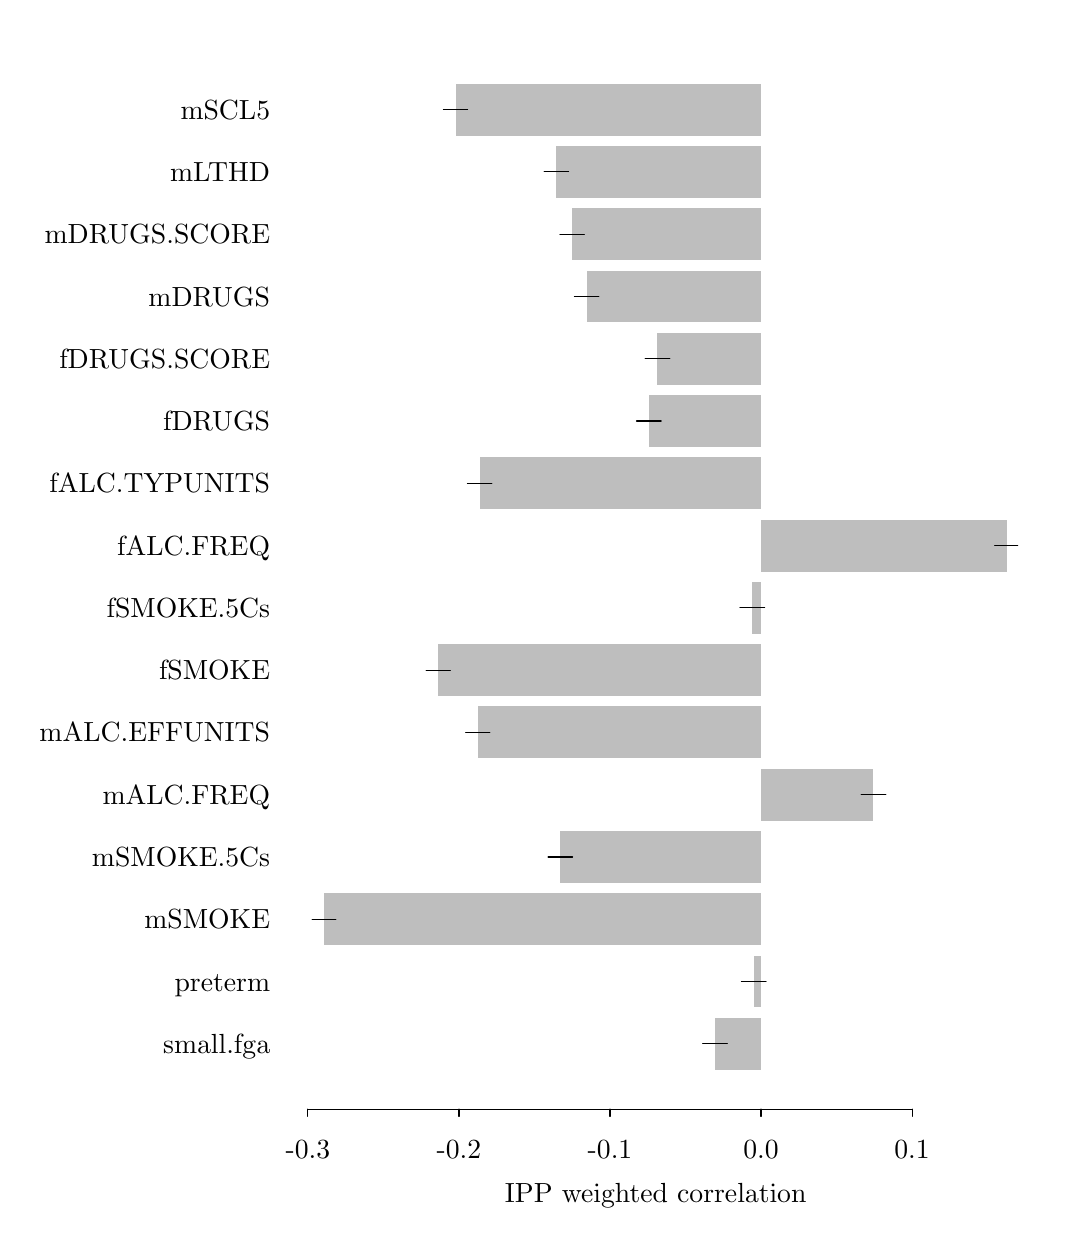
\begin{tikzpicture}[x=1pt,y=1pt]
\definecolor{fillColor}{RGB}{255,255,255}
\path[use as bounding box,fill=fillColor,fill opacity=0.00] (0,0) rectangle (369.89,426.79);
\begin{scope}
\path[clip] (  0.00,  0.00) rectangle (369.89,426.79);
\definecolor{fillColor}{RGB}{190,190,190}

\path[fill=fillColor] (265.00, 50.25) rectangle (248.35, 69.00);

\path[fill=fillColor] (265.00, 72.75) rectangle (262.38, 91.51);

\path[fill=fillColor] (265.00, 95.26) rectangle (107.09,114.01);

\path[fill=fillColor] (265.00,117.76) rectangle (192.47,136.51);

\path[fill=fillColor] (265.00,140.26) rectangle (305.62,159.01);

\path[fill=fillColor] (265.00,162.76) rectangle (162.61,181.52);

\path[fill=fillColor] (265.00,185.27) rectangle (148.37,204.02);

\path[fill=fillColor] (265.00,207.77) rectangle (261.86,226.52);

\path[fill=fillColor] (265.00,230.27) rectangle (353.84,249.02);

\path[fill=fillColor] (265.00,252.77) rectangle (163.31,271.53);

\path[fill=fillColor] (265.00,275.28) rectangle (224.46,294.03);

\path[fill=fillColor] (265.00,297.78) rectangle (227.57,316.53);

\path[fill=fillColor] (265.00,320.28) rectangle (201.99,339.03);

\path[fill=fillColor] (265.00,342.78) rectangle (196.72,361.53);

\path[fill=fillColor] (265.00,365.29) rectangle (191.05,384.04);

\path[fill=fillColor] (265.00,387.79) rectangle (154.60,406.54);
\definecolor{drawColor}{RGB}{0,0,0}

\node[text=drawColor,anchor=base,inner sep=0pt, outer sep=0pt, scale=  1.00] at (226.94,  2.40) {IPP weighted correlation};
\end{scope}
\begin{scope}
\path[clip] (  0.00,  0.00) rectangle (369.89,426.79);
\definecolor{drawColor}{RGB}{0,0,0}

\path[draw=drawColor,line width= 0.4pt,line join=round,line cap=round] (101.27, 36.00) -- (319.58, 36.00);

\path[draw=drawColor,line width= 0.4pt,line join=round,line cap=round] (101.27, 36.00) -- (101.27, 33.38);

\path[draw=drawColor,line width= 0.4pt,line join=round,line cap=round] (155.85, 36.00) -- (155.85, 33.38);

\path[draw=drawColor,line width= 0.4pt,line join=round,line cap=round] (210.43, 36.00) -- (210.43, 33.38);

\path[draw=drawColor,line width= 0.4pt,line join=round,line cap=round] (265.00, 36.00) -- (265.00, 33.38);

\path[draw=drawColor,line width= 0.4pt,line join=round,line cap=round] (319.58, 36.00) -- (319.58, 33.38);

\node[text=drawColor,anchor=base,inner sep=0pt, outer sep=0pt, scale=  1.00] at (101.27, 18.00) {-0.3};

\node[text=drawColor,anchor=base,inner sep=0pt, outer sep=0pt, scale=  1.00] at (155.85, 18.00) {-0.2};

\node[text=drawColor,anchor=base,inner sep=0pt, outer sep=0pt, scale=  1.00] at (210.43, 18.00) {-0.1};

\node[text=drawColor,anchor=base,inner sep=0pt, outer sep=0pt, scale=  1.00] at (265.00, 18.00) {0.0};

\node[text=drawColor,anchor=base,inner sep=0pt, outer sep=0pt, scale=  1.00] at (319.58, 18.00) {0.1};

\node[text=drawColor,anchor=base east,inner sep=0pt, outer sep=0pt, scale=  1.00] at ( 87.60, 56.18) {small.fga};

\node[text=drawColor,anchor=base east,inner sep=0pt, outer sep=0pt, scale=  1.00] at ( 87.60, 78.69) {preterm};

\node[text=drawColor,anchor=base east,inner sep=0pt, outer sep=0pt, scale=  1.00] at ( 87.60,101.19) {mSMOKE};

\node[text=drawColor,anchor=base east,inner sep=0pt, outer sep=0pt, scale=  1.00] at ( 87.60,123.69) {mSMOKE.5Cs};

\node[text=drawColor,anchor=base east,inner sep=0pt, outer sep=0pt, scale=  1.00] at ( 87.60,146.19) {mALC.FREQ};

\node[text=drawColor,anchor=base east,inner sep=0pt, outer sep=0pt, scale=  1.00] at ( 87.60,168.70) {mALC.EFFUNITS};

\node[text=drawColor,anchor=base east,inner sep=0pt, outer sep=0pt, scale=  1.00] at ( 87.60,191.20) {fSMOKE};

\node[text=drawColor,anchor=base east,inner sep=0pt, outer sep=0pt, scale=  1.00] at ( 87.60,213.70) {fSMOKE.5Cs};

\node[text=drawColor,anchor=base east,inner sep=0pt, outer sep=0pt, scale=  1.00] at ( 87.60,236.20) {fALC.FREQ};

\node[text=drawColor,anchor=base east,inner sep=0pt, outer sep=0pt, scale=  1.00] at ( 87.60,258.71) {fALC.TYPUNITS};

\node[text=drawColor,anchor=base east,inner sep=0pt, outer sep=0pt, scale=  1.00] at ( 87.60,281.21) {fDRUGS};

\node[text=drawColor,anchor=base east,inner sep=0pt, outer sep=0pt, scale=  1.00] at ( 87.60,303.71) {fDRUGS.SCORE};

\node[text=drawColor,anchor=base east,inner sep=0pt, outer sep=0pt, scale=  1.00] at ( 87.60,326.21) {mDRUGS};

\node[text=drawColor,anchor=base east,inner sep=0pt, outer sep=0pt, scale=  1.00] at ( 87.60,348.72) {mDRUGS.SCORE};

\node[text=drawColor,anchor=base east,inner sep=0pt, outer sep=0pt, scale=  1.00] at ( 87.60,371.22) {mLTHD};

\node[text=drawColor,anchor=base east,inner sep=0pt, outer sep=0pt, scale=  1.00] at ( 87.60,393.72) {mSCL5};
\end{scope}
\begin{scope}
\path[clip] ( 96.00, 36.00) rectangle (357.89,420.79);
\definecolor{drawColor}{RGB}{0,0,0}

\path[draw=drawColor,line width= 0.4pt,line join=round,line cap=round] (252.81, 59.63) -- (243.89, 59.63);

\path[draw=drawColor,line width= 0.4pt,line join=round,line cap=round] (266.84, 82.13) -- (257.92, 82.13);

\path[draw=drawColor,line width= 0.4pt,line join=round,line cap=round] (111.36,104.63) -- (102.82,104.63);

\path[draw=drawColor,line width= 0.4pt,line join=round,line cap=round] (196.90,127.13) -- (188.05,127.13);

\path[draw=drawColor,line width= 0.4pt,line join=round,line cap=round] (310.07,149.64) -- (301.17,149.64);

\path[draw=drawColor,line width= 0.4pt,line join=round,line cap=round] (167.00,172.14) -- (158.23,172.14);

\path[draw=drawColor,line width= 0.4pt,line join=round,line cap=round] (152.73,194.64) -- (144.01,194.64);

\path[draw=drawColor,line width= 0.4pt,line join=round,line cap=round] (266.32,217.14) -- (257.40,217.14);

\path[draw=drawColor,line width= 0.4pt,line join=round,line cap=round] (358.25,239.65) -- (349.44,239.65);

\path[draw=drawColor,line width= 0.4pt,line join=round,line cap=round] (167.69,262.15) -- (158.92,262.15);

\path[draw=drawColor,line width= 0.4pt,line join=round,line cap=round] (228.91,284.65) -- (220.01,284.65);

\path[draw=drawColor,line width= 0.4pt,line join=round,line cap=round] (232.02,307.15) -- (223.11,307.15);

\path[draw=drawColor,line width= 0.4pt,line join=round,line cap=round] (206.42,329.66) -- (197.56,329.66);

\path[draw=drawColor,line width= 0.4pt,line join=round,line cap=round] (201.14,352.16) -- (192.29,352.16);

\path[draw=drawColor,line width= 0.4pt,line join=round,line cap=round] (195.47,374.66) -- (186.63,374.66);

\path[draw=drawColor,line width= 0.4pt,line join=round,line cap=round] (158.97,397.16) -- (150.23,397.16);
\end{scope}
\end{tikzpicture}

	\caption{Inverse probability of participation weighted correlations based on MoBa data. See supplementary discussion for details.}
	\label{fig:educors}
\end{figure}

\newpage

\section{Supplementary discussion}
\subsection{Implied conditional independencies}
In the main text we use \emph{genetic correlations} between exposures and participation predictors to argue that a causal structure in which these variables are correlated in the population is more plausible than a causal structure in which these variables are uncorrelated. This is a central argument, because only if exposures and participation predictors are correlated in the population, can inverse probability weighting be superior to adjusting for participation predictors. More specifically, given the presence of a common unobserved cause of participation predictors $L$ and the outcome $D$ ($L \leftarrow U \rightarrow D$), IPPW is superior when $E$ and $L$ have an unobserved common cause ($E \leftarrow U^* \rightarrow L$) , or when $E$ causes $L$ ($E \leftarrow L$). When $L$ causes $E$, or there is no direct relationship between $L$ and $E$, AR is superior.

As an alternative to \emph{genetic correlations} one can uses implied (conditional) independencies to check consistency between data an a hypothesized causal structure. The analysis of Figures \emph{1a} and \emph{1b} shows that disorder $D$ should be independent of participation $P$ given exposure $E$ and participation predictors $L$ ($D \bot P|E,L$) for \emph{1a} and $D \bot P | E$ for \emph{1b}. Both conditional independencies are present in our data. However, only Figure \emph{1a} and not \emph{1b} implies independence of $L$ and $E$ ($E \bot L$) in the study population (in \emph{1a} only conditioning on $P$ opens a path between $E$ and $L$). To evaluate the association between $E$ and $L$ in the population one can either calculate weighted correlations between these variables using the study sample, or investigate auxiliary data. Figure \ref{fig:educors} shows that weighted correlations between $E$ and $L$ were with a few exceptions substantial. 

Because $E$ and $L$ are dependent in the study sample, the analysis of implied conditional independencies shows that the causal structure in \emph{1b} is a better description of the data obtained from MoBa participants. Therefore, even without the additional information from genetic correlations, the available evidence suggests that the causal structure in \emph{1b} rather than \emph{1a} describes our data better. (Which implies that adjustment for participation predictors will not reduce selection bias).



%\begin{figure}
%	\centering
%	\begin{singlespace}
%		\resizebox{\textwidth}{!}{
\begin{tikzpicture}
	[
	 sibling distance = 4cm,
	 level distance   = 4cm,
	 every node/.style = {shape=rectangle,
		                  draw,
		                  align=center,
		                  top color = white,
	                      font=\footnotesize,
	                      minimum size = 22mm,
	                      text width = 28mm,
	                      inner sep = 0pt
                         },
    L1/.style ={sibling distance=9cm},
    L2/.style ={sibling distance=5cm},
    L3/.style ={sibling distance=3cm},
    YN/.style = {minimum size = 8mm,
    	text width = 8mm,
    	pos = .5,
    	text opacity = 1,
    	fill opacity=0}
	]
	
	\newcommand{\LP}{Is there a participation indicator $L$?}
	\newcommand{\nB}{Bias is unlikely}
	\newcommand{\LED}{Does $L$ modify the effect of the exposure
		             on the outcome }
	\newcommand{\EL}{Does the expo- sure cause
		             or share a common unobserved
		             cause with $L$?}
    \newcommand{\EP}{Is participation $P$
    	             an effect of
    	             the exposure $E$?}
    \newcommand{\CCDL}{Do outcome $D$ and $L$
    	               have an unobserved
    	               common cause $U$?}	
	\node (A) {\LP}
	child [L2] {[] node  (B1) {\LED}
				child [L1] {[] node (C1) {\EP}
					        child [L2] {[] node (Dx1) {\EL}
					        	        child [L2] {[] node (Ex1) {\CCDL}
					        	        	        child [L2] {[rounded corners=3mm] node (Fx1) {IPPW}}
					        	        	        child [L2] {[rounded corners=3mm] node (Fx2) {DS/MRP, IPPW}}
					        	                                         }
					        	        child [L2] {[rounded corners=3mm] node (Ex2) {DS/MRP, IPPW}}
					                                       }
					        child [L2] {[rounded corners=3mm] node (Dx2) {DS/MRP, IPPW}}
				                              }
			    child [L1] {[] node (C2) {\CCDL}
		                    child [L2] {[] node (D1) {\EL}
		                    	        child [L2] {[rounded corners=3mm] node (E1) {IPPW}}
		                    	        child [L2] {[] node (E2) {\EP}
		                    	        	        child [L2] {[rounded corners=3mm] node (F1) {AR, DS/MRP, IPPW}}
		                    	        	        child [L2] {[rounded corners=3mm] node (F2) {\nB}}
		                    	                                      }
		                                                  }
		                    child [L2] {[rounded corners=3mm] node (D2) {\nB}}                    
	                                         }}
	child [L2] {[rounded corners=3mm] node  (B2) {\nB}};
	
	 \begin{scope}[nodes = {draw = none}]
	   \path (A)  -- (B1) node [YN, left]   {Yes};
	   \path (A)  -- (B2) node [YN, right]  {No};
	   \path (B1) -- (C1) node [YN, left]   {Yes};
	   \path (B1) -- (C2) node [YN, right]  {No};
	   \path (C2) -- (D1) node [YN, left]   {Yes};
	   \path (C2) -- (D2) node [YN, right]  {No};
	   \path (D1) -- (E1) node [YN, left]   {Yes};
	   \path (D1) -- (E2) node [YN, right]  {No};
	   \path (E2) -- (F1) node [YN, left]   {Yes};
	   \path (E2) -- (F2) node [YN, right]  {No};
	   \path (Dx1) -- (Ex1) node [YN, left]   {Yes};
	   \path (Dx1) -- (Ex2) node [YN, right]  {No};
	   \path (C1) -- (Dx1) node [YN, left]   {Yes};
	   \path (C1) -- (Dx2) node [YN, right]  {No};
	   \path (Ex1) -- (Fx1) node [YN, left]   {Yes};
	   \path (Ex1) -- (Fx2) node [YN, right]  {No};
	 \end{scope}
\end{tikzpicture}}
%	\end{singlespace}
	
	%
\begin{tikzpicture}
	[
	 sibling distance = 4cm,
	 level distance   = 4cm,
	 every node/.style = {shape=rectangle,
		                  draw,
		                  align=center,
		                  top color = white,
	                      font=\footnotesize,
	                      minimum size = 22mm,
	                      text width = 28mm,
	                      inner sep = 0pt
                         },
    L1/.style ={sibling distance=9cm},
    L2/.style ={sibling distance=5cm},
    L3/.style ={sibling distance=3cm},
    YN/.style = {minimum size = 8mm,
    	text width = 8mm,
    	pos = .5,
    	text opacity = 1,
    	fill opacity=0}
	]
	
	\newcommand{\LP}{Is there a participation indicator $L$?}
	\newcommand{\nB}{Bias is unlikely}
	\newcommand{\LED}{Does $L$ modify the effect of the exposure
		             on the outcome }
	\newcommand{\EL}{Does the expo- sure cause
		             or share a common unobserved
		             cause with $L$?}
    \newcommand{\EP}{Is participation $P$
    	             an effect of
    	             the exposure $E$?}
    \newcommand{\CCDL}{Do outcome $D$ and $L$
    	               have an unobserved
    	               common cause $U$?}	
	\node (A) {\LP}
	child [L2] {[] node  (B1) {\LED}
				child [L1] {[] node (C1) {\EP}
					        child [L2] {[] node (Dx1) {\EL}
					        	        child [L2] {[] node (Ex1) {\CCDL}
					        	        	        child [L2] {[rounded corners=3mm] node (Fx1) {IPPW}}
					        	        	        child [L2] {[rounded corners=3mm] node (Fx2) {DS/MRP, IPPW}}
					        	                                         }
					        	        child [L2] {[rounded corners=3mm] node (Ex2) {DS/MRP, IPPW}}
					                                       }
					        child [L2] {[rounded corners=3mm] node (Dx2) {DS/MRP, IPPW}}
				                              }
			    child [L1] {[] node (C2) {\CCDL}
		                    child [L2] {[] node (D1) {\EL}
		                    	        child [L2] {[rounded corners=3mm] node (E1) {IPPW}}
		                    	        child [L2] {[] node (E2) {\EP}
		                    	        	        child [L2] {[rounded corners=3mm] node (F1) {AR, DS/MRP, IPPW}}
		                    	        	        child [L2] {[rounded corners=3mm] node (F2) {\nB}}
		                    	                                      }
		                                                  }
		                    child [L2] {[rounded corners=3mm] node (D2) {\nB}}                    
	                                         }}
	child [L2] {[rounded corners=3mm] node  (B2) {\nB}};
	
	 \begin{scope}[nodes = {draw = none}]
	   \path (A)  -- (B1) node [YN, left]   {Yes};
	   \path (A)  -- (B2) node [YN, right]  {No};
	   \path (B1) -- (C1) node [YN, left]   {Yes};
	   \path (B1) -- (C2) node [YN, right]  {No};
	   \path (C2) -- (D1) node [YN, left]   {Yes};
	   \path (C2) -- (D2) node [YN, right]  {No};
	   \path (D1) -- (E1) node [YN, left]   {Yes};
	   \path (D1) -- (E2) node [YN, right]  {No};
	   \path (E2) -- (F1) node [YN, left]   {Yes};
	   \path (E2) -- (F2) node [YN, right]  {No};
	   \path (Dx1) -- (Ex1) node [YN, left]   {Yes};
	   \path (Dx1) -- (Ex2) node [YN, right]  {No};
	   \path (C1) -- (Dx1) node [YN, left]   {Yes};
	   \path (C1) -- (Dx2) node [YN, right]  {No};
	   \path (Ex1) -- (Fx1) node [YN, left]   {Yes};
	   \path (Ex1) -- (Fx2) node [YN, right]  {No};
	 \end{scope}
\end{tikzpicture}
%	\caption{Decision tree for identification of selection bias and choice of approach to correct it. See Figure 1 in main text for causal diagrams that underlie the decision tree. 
%	To determine if selection bias is likely, and if so which correction method can be used, proceed through the questions from the top on. Ending in a node "Bias is unlikely" implies that an  analysis without correction for selection bias will still result in estimates with out selection bias. Otherwise, different correction types can be used, depending on the underlying causal structure. IPPW stands for analysis with inverse probability of participation weighting, DS for direct standardization and MRP for multilevel regression and post stratification AR for adjusted regression.}
%	\label{fig:DecisionTree}
%\end{figure}


\printbibliography

\end{document}
